\documentclass{mimosis}
\usepackage{algorithm}
\usepackage[noend]{algpseudocode}
\usepackage{amsfonts}
\usepackage[toc,page]{appendix}
\usepackage{bm}
\usepackage{chngcntr}
\usepackage[ngerman,english]{cleveref}
\usepackage{environ}
\usepackage{numprint}
\usepackage[super]{nth}
\usepackage{placeins}
\usepackage{svg}
\usepackage{tikz}
\usepackage[textsize=footnotesize]{todonotes}

\usetikzlibrary{arrows, arrows.meta, calc, decorations.pathreplacing, patterns,
positioning}

%%% Cleveref settings %%%
\Crefname{equation}{Eq.}{Eqs.}
\newcommand{\crefrangeconjunction}{--}
\AtBeginEnvironment{appendices}{
\crefalias{section}{appendix}
\crefalias{Section}{Appendix}
\crefalias{chapter}{appendix}
\crefalias{Chapter}{Appendix}
}

%%% Numprint settings %%%
\npthousandsep{,}%
\npdecimalsign{.}%
\npproductsign{\cdot}%
\npunitseparator{\,}%
\npdegreeseparator{}%
\npcelsiusseparator{\nprt@unitsep}%
\nppercentseparator{\nprt@unitsep}%

% shorter minus sign in \numprint exponents
\expandafter\renewcommand\csname nprt@sign@-\endcsname{%
\ifmmode {-}\else {\text{-}}\fi}

%%% Hyphenation %%%
\hyphenation{Page-Rank net-works}

% Avoid resetting footnotes after each part/chapter
%\makeatletter
%\pretocmd{\@schapter}{\setcounter{footnote}{0}}{}{}
\counterwithout*{footnote}{chapter}
%\pretocmd{\@chapter}{\setcounter{footnote}{0}}{}{}
%\makeatother

%%% Macros %%%
%%%%%%%%%%%%%%%%%%%%%%%%%%%%%%%%%%%%%%%%%%%%%%%%%%%%%%%%%%%%%%%%%%%%%%%%
% Colors
%%%%%%%%%%%%%%%%%%%%%%%%%%%%%%%%%%%%%%%%%%%%%%%%%%%%%%%%%%%%%%%%%%%%%%%%
\newcommand{\darkgreen}{black!60!green}
\newcommand{\darkorange}{brown!70!orange}

%%%%%%%%%%%%%%%%%%%%%%%%%%%%%%%%%%%%%%%%%%%%%%%%%%%%%%%%%%%%%%%%%%%%%%%%
% Chapter paragraphs
%%%%%%%%%%%%%%%%%%%%%%%%%%%%%%%%%%%%%%%%%%%%%%%%%%%%%%%%%%%%%%%%%%%%%%%%
\newcommand{\bibnotes}[1]{\paragraph{Bibliographic Notes}#1}

%%%%%%%%%%%%%%%%%%%%%%%%%%%%%%%%%%%%%%%%%%%%%%%%%%%%%%%%%%%%%%%%%%%%%%%%
% Writing
%%%%%%%%%%%%%%%%%%%%%%%%%%%%%%%%%%%%%%%%%%%%%%%%%%%%%%%%%%%%%%%%%%%%%%%%
\newcommand{\eg}{e.g.,\xspace}
\newcommand{\ie}{i.e.,\xspace}
\newcommand{\etal}{et al.\xspace}
\newcommand{\etc}{etc.\xspace}
\newcommand{\wrt}{w.r.t.\xspace} \newcommand{\aka}{a.k.a.\xspace}
\renewcommand{\th}{\textsuperscript{\textup{th}}\xspace}
\newcommand{\wilog}{w.l.o.g.\xspace}
\newcommand{\Wilog}{W.l.o.g.\xspace}
\newcommand{\np}{\ensuremath{\mathcal{NP}}}
\newcommand{\apxch}[1]{\chapter{Appendix of \Cref{#1}}}
\newcommand{\alenex}[2]{
\textit{#1 Workshop on Algorithm Engineering and Experiments (ALENEX #2)}}

%%%%%%%%%%%%%%%%%%%%%%%%%%%%%%%%%%%%%%%%%%%%%%%%%%%%%%%%%%%%%%%%%%%%%%%%
% Math
%%%%%%%%%%%%%%%%%%%%%%%%%%%%%%%%%%%%%%%%%%%%%%%%%%%%%%%%%%%%%%%%%%%%%%%%
\newcommand{\set}[1]{\ensuremath{\left\lbrace#1\right\rbrace}}
\renewcommand{\iff}{\ensuremath{\Leftrightarrow}}
\newcommand{\Oh}{\ensuremath{\mathcal{O}}}
\newcommand{\fdist}{\ensuremath{\zeta}}
\newcommand{\fdistp}{\ensuremath{\fdist_{\alpha}}}
\newcommand{\ct}{\ensuremath{t_c}}
\newcommand{\ctg}{\ensuremath{t_{c, G}}}
\newcommand{\hitt}{\ensuremath{t_h}}
\newcommand{\expected}[1]{\ensuremath{\mathbf{E}\left[#1\right]}}
\DeclareMathOperator{\gmean}{GM}
\DeclareMathOperator*{\argmax}{argmax}
\DeclareMathOperator*{\argmin}{argmin}
\newcommand{\norm}[1]{\left\lVert#1\right\rVert}
\newcommand{\onenorm}[1]{\left\lVert#1\right\rVert_1}
\newcommand{\twonorm}[1]{\left\lVert#1\right\rVert_2}
\newcommand{\maxnorm}[1]{\left\lVert#1\right\rVert_{\infty}}
\newcommand{\natn}{\ensuremath{\mathbb{N}}}
\newcommand{\ratn}{\ensuremath{\mathbb{Q}}}
\newcommand{\pair}[2]{\ensuremath{\left<#1, #2\right>}}
\newcommand{\poly}{\text{poly}}
\newcommand{\lonerel}{\ensuremath{\mathrm{L1}_\mathrm{rel}}}
\newcommand{\ltworel}{\ensuremath{\mathrm{L2}_\mathrm{rel}}}
\newcommand{\erel}{\ensuremath{\mathrm{E}_\mathrm{rel}}}

\renewcommand{\epsilon}{\varepsilon}

%%%%%%%%%%%%%%%%%%%%%%%%%%%%%%%%%%%%%%%%%%%%%%%%%%%%%%%%%%%%%%%%%%%%%%%%
% Graph Measures
%%%%%%%%%%%%%%%%%%%%%%%%%%%%%%%%%%%%%%%%%%%%%%%%%%%%%%%%%%%%%%%%%%%%%%%%
\newcommand{\vol}{\ensuremath{\text{vol}}}
\newcommand{\nout}{\ensuremath{N_{\text{out}}}}
\newcommand{\nin}{\ensuremath{N_{\text{in}}}}
\newcommand{\degin}{\ensuremath{\deg_{\text{in}}}}
\newcommand{\degout}{\ensuremath{\deg_{\text{out}}}}
\newcommand{\diam}{\ensuremath{\text{diam}}}
\newcommand{\ecc}{\ensuremath{\text{ecc}}}
\newcommand{\kidx}{\ensuremath{\mathcal{K}}}

%%%%%%%%%%%%%%%%%%%%%%%%%%%%%%%%%%%%%%%%%%%%%%%%%%%%%%%%%%%%%%%%%%%%%%%%
% Formatting numbers
%%%%%%%%%%%%%%%%%%%%%%%%%%%%%%%%%%%%%%%%%%%%%%%%%%%%%%%%%%%%%%%%%%%%%%%%
\newcommand{\onedigit}[1]{
\ensuremath{\num[round-mode=places,round-precision=1]{#1}}
}

%%%%%%%%%%%%%%%%%%%%%%%%%%%%%%%%%%%%%%%%%%%%%%%%%%%%%%%%%%%%%%%%%%%%%%%%
% Parentheses
%%%%%%%%%%%%%%%%%%%%%%%%%%%%%%%%%%%%%%%%%%%%%%%%%%%%%%%%%%%%%%%%%%%%%%%%
\newcommand{\roundb}[1]{\ensuremath{\left(#1\right)}}
\newcommand{\ceil}[1]{\ensuremath{\left\lceil#1\right\rceil}}

%%%%%%%%%%%%%%%%%%%%%%%%%%%%%%%%%%%%%%%%%%%%%%%%%%%%%%%%%%%%%%%%%%%%%%%%
% Matrices and Vectors
%%%%%%%%%%%%%%%%%%%%%%%%%%%%%%%%%%%%%%%%%%%%%%%%%%%%%%%%%%%%%%%%%%%%%%%%
\newcommand{\mat}[1]{\ensuremath{\mathbf{#1}}\xspace}
\newcommand{\vect}[1]{\ensuremath{\mathbf{#1}}\xspace}
\newcommand{\Adj}{\mat{A}}
\newcommand{\Deg}{\mat{D}}
\newcommand{\Ones}{\mat{J}}
\newcommand{\ones}{\mat{j}}
\newcommand{\Ident}{\mat{I}}
\newcommand{\Fmat}{\ensuremath{\bm{\Omega}}\xspace}
\newcommand{\Fmatapx}{\ensuremath{\widetilde{\Fmat}}\xspace}
\newcommand{\Fmatp}{\ensuremath{\bm{\Omega}_{\alpha}}\xspace}
\newcommand{\cunit}[1]{\ensuremath{\vect{e}_{#1}}}
\newcommand{\diag}[1]{\ensuremath{\text{diag}\roundb{#1}}\xspace}
\newcommand{\tr}[1]{\ensuremath{\text{tr}\roundb{#1}}\xspace}
\newcommand{\xapprox}{\ensuremath{\widetilde{\vect{x}}}}

%%%%%%%%%%%%%%%%%%%%%%%%%%%%%%%%%%%%%%%%%%%%%%%%%%%%%%%%%%%%%%%%%%%%%%%%
% Effective Resistance Notation
%%%%%%%%%%%%%%%%%%%%%%%%%%%%%%%%%%%%%%%%%%%%%%%%%%%%%%%%%%%%%%%%%%%%%%%%
\newcommand{\reff}{\ensuremath{r_{\text{eff}}}\xspace}
\newcommand{\ceff}{\ensuremath{c_{\text{eff}}}\xspace}
\newcommand{\rdist}{\ensuremath{\rho}\xspace}
\newcommand{\rdistapx}{\ensuremath{\tilde{\rho}}\xspace}
\newcommand{\rdiststar}{\ensuremath{\rho_{\star}}\xspace}
\newcommand{\rdiststarapx}{\ensuremath{\tilde{\rho}_{\star}}\xspace}
\newcommand{\Lapl}{\mat{L}}
\newcommand{\Lstar}{\mat{L_{\star}}}
\newcommand{\Linv}{\ensuremath{\Lapl^\dagger}\xspace}
\newcommand{\Linvstar}{\ensuremath{\Lapl^\dagger_\star}\xspace}
\newcommand{\Linvapx}{\ensuremath{\widetilde{\Lapl^\dagger}}\xspace}

%%%%%%%%%%%%%%%%%%%%%%%%%%%%%%%%%%%%%%%%%%%%%%%%%%%%%%%%%%%%%%%%%%%%%%%%
% Centrality Measures
%%%%%%%%%%%%%%%%%%%%%%%%%%%%%%%%%%%%%%%%%%%%%%%%%%%%%%%%%%%%%%%%%%%%%%%%
\newcommand{\clos}{\ensuremath{c_c}\xspace}
\newcommand{\farn}{\ensuremath{f}\xspace}
\newcommand{\elfarn}{\ensuremath{f_e}\xspace}
\newcommand{\ffarnp}{\ensuremath{f_{f, \alpha}}\xspace}
\newcommand{\ffarn}{\ensuremath{f_f}\xspace}
\newcommand{\harm}{\ensuremath{c_h}}
\newcommand{\harmupp}{\ensuremath{\widetilde{\harm}}}
\newcommand{\betw}{\ensuremath{c_b}\xspace}
\newcommand{\bapx}{\ensuremath{\tilde{c}_b}\xspace}
\newcommand{\nrwb}{\ensuremath{c_{\text{nrwb}}}\xspace}
\newcommand{\katz}{\ensuremath{c_{\text{K}}}}
\newcommand{\edw}{ED-Walk\xspace}
\newcommand{\ed}{\ensuremath{c_{\text{ED}}}}
\newcommand{\eig}{\ensuremath{c_{\text{eig}}}}
\newcommand{\pr}{\ensuremath{c_{\text{PR}}}}
\newcommand{\elclos}{\ensuremath{c_e}}
\newcommand{\fclos}{\ensuremath{c_f}}
\newcommand{\fclosp}{\ensuremath{c_{f,\alpha}}}

\newcommand{\gdeg}{\ensuremath{g_d}\xspace}
\newcommand{\gclos}{\ensuremath{g_c}\xspace}
\newcommand{\gfarn}{\ensuremath{g_f}\xspace}
\newcommand{\gffarn}{\ensuremath{g_{\mathit{ff}}\xspace}}
\newcommand{\gffarnp}{\ensuremath{g_{\mathit{ff},\alpha}\xspace}}
\newcommand{\gharm}{\ensuremath{g_h}\xspace}
\newcommand{\gfclos}{\ensuremath{g_{\mathit{fc}}}\xspace}
\newcommand{\gfclosp}{\ensuremath{g_{\mathit{fc},\alpha}}\xspace}
\newcommand{\gharmupp}{\ensuremath{\widehat{\gharm}}\xspace}
\newcommand{\gfarnapx}{\ensuremath{\widetilde{\gfarn}}\xspace}
\newcommand{\gfarnupp}{\ensuremath{\widehat{\gfarn}}\xspace}
\newcommand{\ged}{\ensuremath{g_{\text{ED}}}}
\newcommand{\gedll}{\ensuremath{g_{\text{ED}}^{\le\ell}}}
\newcommand{\gedgl}{\ensuremath{g_{\text{ED}}^{>\ell}}}

%%%%%%%%%%%%%%%%%%%%%%%%%%%%%%%%%%%%%%%%%%%%%%%%%%%%%%%%%%%%%%%%%%%%%%%%
% Specific Notations
%%%%%%%%%%%%%%%%%%%%%%%%%%%%%%%%%%%%%%%%%%%%%%%%%%%%%%%%%%%%%%%%%%%%%%%%
\newcommand{\dcut}{\ensuremath{d_{\text{cut}}}}
\newcommand{\isexact}{\texttt{isExact}\xspace}
\newcommand{\imax}{\ensuremath{i_{\max}}\xspace}
\newcommand{\Suv}{\ensuremath{S_{-u}^{+v}}}
\newcommand{\Su}{\ensuremath{S_{-u}}}
\newcommand{\Sv}{\ensuremath{S^{+v}}}
\newcommand{\deltafarnm}{\ensuremath{\Delta^-}}
\newcommand{\deltafarnp}{\ensuremath{\Delta^+}}
\newcommand{\Huvp}{\ensuremath{H_{u, v}^+}}
\newcommand{\Huvm}{\ensuremath{H_{u, v}^-}}
\newcommand{\Luvo}{\ensuremath{L_{u, v}^0}}
\newcommand{\Huvo}{\ensuremath{H_{u, v}^0}}
\newcommand{\wmin}{\ensuremath{w_{\min}}}
\newcommand{\wmax}{\ensuremath{w_{\max}}}
\newcommand{\PhiSu}{\ensuremath{\Phi_{S, u}}}
\newcommand{\PhiSv}{\ensuremath{\Phi_{S, v}}}
\newcommand{\phit}{\ensuremath{\phi^{\text{hit}}}}
\newcommand{\pmiss}{\ensuremath{\phi^{\text{miss}}}}
\newcommand{\pshit}{\ensuremath{\psi^{\text{hit}}}}
\newcommand{\psmiss}{\ensuremath{\psi^{\text{miss}}}}
\newcommand{\degmax}{\ensuremath{\deg_{\max}}}
\newcommand{\erdosr}{Erd\H{o}s R\'enyi\xspace}
\newcommand{\interm}{\ensuremath{^{(i)}}\xspace}
\newcommand{\iinterm}{\ensuremath{^{(ii)}}\xspace}
\newcommand{\final}{\ensuremath{^{(f)}}\xspace}
\newcommand{\iteri}{^{[i]}}
\newcommand{\iter}[1]{^{[#1]}}

\newcommand{\tdis}{\ensuremath{t_{\text{dis}}}}
\newcommand{\tfin}{\ensuremath{t_{\text{fin}}}}
\newcommand{\gstar}{\ensuremath{G_{\star}}\xspace}
\newcommand{\gstarp}{\ensuremath{G_{\star,\alpha}}\xspace}

\newcommand{\graphfh}{edge factor 16, $a = \numprint{0.57}, b =
\numprint{0.19}, c = \numprint{0.19},$ and $d = \numprint{0.05}$\xspace}

\DeclareMathOperator{\rlxmove}{\gets_\mathsf{relaxed}}
\DeclareMathOperator{\loadacq}{\gets_\mathsf{acquire}}
\DeclareMathOperator{\storerel}{\gets_\mathsf{release}}

%%%%%%%%%%%%%%%%%%%%%%%%%%%%%%%%%%%%%%%%%%%%%%%%%%%%%%%%%%%%%%%%%%%%%%%%
% Tools
%%%%%%%%%%%%%%%%%%%%%%%%%%%%%%%%%%%%%%%%%%%%%%%%%%%%%%%%%%%%%%%%%%%%%%%%
\newcommand{\nwkurl}{\url{https://github.com/networkit/networkit/}\xspace}

%%%%%%%%%%%%%%%%%%%%%%%%%%%%%%%%%%%%%%%%%%%%%%%%%%%%%%%%%%%%%%%%%%%%%%%%
% Tikz
%%%%%%%%%%%%%%%%%%%%%%%%%%%%%%%%%%%%%%%%%%%%%%%%%%%%%%%%%%%%%%%%%%%%%%%%
\newcommand{\vertex}[2]{\node[minimum size=5mm,circle,draw] (#2) at (#1) {#2};}
\newcommand{\filledvertex}[1]{\draw[fill] (#1) circle [radius=2pt];}
\newcommand{\edge}[2]{\draw[-] (#1) -- (#2);}
\newcommand{\myarrow}{\draw[-{latex[scale=2]}]}
\newcommand{\myarrowcolor}[1]{\draw[-{latex[scale=2]},#1]}
\newcommand{\mydoublearrow}{\draw[latex'-latex']}
\newcommand{\dedge}[2]{\myarrow (#1) -- (#2);}
\newcommand{\dedgecolor}[3]{\myarrowcolor{#3} (#1) -- (#2);}
\newcommand{\dbedge}[3]{\myarrow (#1) edge [#3] node {} (#2);}
\newcommand{\ddedge}[2]{\mydoublearrow (#1) -- (#2);}
\newcommand{\thickedge}[2]{\draw[-, line width=.4mm] (#1) -- (#2);}
\newcommand{\dashedEdge}[2]{\draw[dashed] (#1) -- (#2);}
\newcommand{\dottedEdge}[2]{\draw[dotted] (#1) -- (#2);}
\newcommand{\dashdottedEdge}[2]{\draw[dash dot] (#1) -- (#2);}
\newcommand{\eqnode}[2]{
\node[] at (#1){\begin{minipage}{\textwidth}#2\end{minipage}};
}
\tikzstyle{graphnode}=[circle,draw,thick]
\tikzstyle{groupstyle}=[dashed, thick]
\newcommand{\simplenode}[2]{\node[graphnode] (#1) at (#2) {};}
\newcommand{\colornode}[2]{\node[graphnode, \darkorange] (#1) at (#2) {};}
\newcommand{\customcolornode}[3]{\node[graphnode,fill, #3,thick,draw=black] (#1) at (#2) {};}
\newcommand{\colortextnode}[3]{\node[graphnode, \darkorange] (#1) at (#2) {#3};}
\newcommand{\textnode}[3]{\node[graphnode, minimum size=4mm] (#1) at (#2) {#3};}
\newcommand{\textnodecolor}[4]{\node[graphnode, minimum size=4mm,fill,#4] (#1) at (#2) {#3};}
\newcommand{\nshift}{5pt}

%%%%%%%%%%%%%%%%%%%%%%%%%%%%%%%%%%%%%%%%%%%%%%%%%%%%%%%%%%%%%%%%%%%%%%%%
% Functions and Algorithms
%%%%%%%%%%%%%%%%%%%%%%%%%%%%%%%%%%%%%%%%%%%%%%%%%%%%%%%%%%%%%%%%%%%%%%%%
\newcommand{\func}[1]{\textsf{#1}\xspace}
\newcommand{\nbcut}{\func{NBCut}}
\newcommand{\bfscut}{\func{BFScut}}
\newcommand{\nbbound}{\func{NBBound}}
\newcommand{\bfsbound}{\func{BFSbound}}
\newcommand{\localswaps}{\textit{Local-Swaps}\xspace}
\newcommand{\growshrink}{\textit{Grow-Shrink}\xspace}
\newcommand{\greedyh}{\func{Greedy-H}}
\newcommand{\greedylsh}{\func{Greedy-LS-H}}
\newcommand{\bestrandomh}{\func{Best-Random-H}}
\newcommand{\greedyc}{\func{Greedy-C}}
\newcommand{\gs}{\func{GS}}
\newcommand{\bestrandomc}{\func{Best-Random-C}}
\newcommand{\greedylsc}{\func{Greedy-LS-C}}
\newcommand{\gslsc}{\func{GS-LS-C}}
\newcommand{\ust}{\func{UST}}
\newcommand{\lamgjlt}{\func{Lamg-jlt}}
\newcommand{\juliajlt}{\func{Julia-jlt}}
\newcommand{\jltjulia}{\func{JLT-Julia}}
\newcommand{\jltcpp}{\func{JLT-CPP}}
\newcommand{\bekas}{\func{Bekas}}
\newcommand{\bekash}{\func{Bekas-h}}
\newcommand{\suitor}{\func{Suitor}}
\newcommand{\dynmwmrandom}{\func{DynMWMRandom}}
\newcommand{\ssuitor}{\func{SortSuitor}}
\newcommand{\findsuitor}{\func{findSuitor}}
\newcommand{\findaff}{\func{findAffected}}
\newcommand{\findaffb}{$\func{findAffected}_B$\xspace}
\newcommand{\updateaff}{\func{updateAffected}}
\newcommand{\affected}{\ensuremath{\mathit{affected}}\xspace}
\newcommand{\heaviest}{\ensuremath{\mathit{heaviest}}\xspace}
\newcommand{\partner}{\ensuremath{\mathit{partner}}\xspace}
\newcommand{\done}{\ensuremath{\mathit{done}}\xspace}
\newcommand{\vsuitor}{\ensuremath{\mathit{suitor}}\xspace}
\newcommand{\cur}{\ensuremath{\mathit{cur}}\xspace}
\newcommand{\mate}{\ensuremath{\mathit{mate}}\xspace}
\newcommand{\nextCand}{\texttt{nextCandidate}\xspace}

\newcommand{\localframe}{\textit{local-frame}\xspace}
\newcommand{\Localframe}{\textit{Local-frame}\xspace}
\newcommand{\sharedframe}{\textit{shared-frame}\xspace}
\newcommand{\Sharedframe}{\textit{Shared-frame}\xspace}
\newcommand{\indexedframe}{\textit{indexed-frame}\xspace}
\newcommand{\Indexedframe}{\textit{Indexed-frame}\xspace}
\newcommand{\kadabra}{\func{KADABRA}}
\newcommand{\rk}{\func{RK}}

%%%%%%%%%%%%%%%%%%%%%%%%%%%%%%%%%%%%%%%%%%%%%%%%%%%%%%%%%%%%%%%%%%%%%%%%
% Pseudocode
%%%%%%%%%%%%%%%%%%%%%%%%%%%%%%%%%%%%%%%%%%%%%%%%%%%%%%%%%%%%%%%%%%%%%%%%
\newcommand{\topk}{\texttt{TopK}\xspace}
\newcommand{\prioq}{\texttt{PrioQ}\xspace}
\newcommand{\true}{\texttt{true}\xspace}
\newcommand{\false}{\texttt{false}\xspace}
\newcommand{\nil}{\texttt{null}\xspace}
\newcommand{\didswap}{\texttt{didSwap}\xspace}
\newcommand{\TopComment}[1]{\State\texttt{/* #1 */}}

%%%%%%%%%%%%%%%%%%%%%%%%%%%%%%%%%%%%%%%%%%%%%%%%%%%%%%%%%%%%%%%%%%%%%%%%
% Cluster specs
%%%%%%%%%%%%%%%%%%%%%%%%%%%%%%%%%%%%%%%%%%%%%%%%%%%%%%%%%%%%%%%%%%%%%%%%
\newcommand{\RAM}{$\SI{192}{\gibi\byte}$ of RAM\xspace}
\newcommand{\cpumodel}{Intel Xeon Gold 6126\xspace}
\newcommand{\CPU}{\cpumodel with $2\times12$ cores\xspace}
\newcommand{\egocpu}{Intel Xeon Gold 6154\xspace}
\newcommand{\egoram}{$\SI{1.5}{\tebi\byte}$ of RAM\xspace}

%%%%%%%%%%%%%%%%%%%%%%%%%%%%%%%%%%%%%%%%%%%%%%%%%%%%%%%%%%%%%%%%%%%%%%%%
% Changed text after first submission
%%%%%%%%%%%%%%%%%%%%%%%%%%%%%%%%%%%%%%%%%%%%%%%%%%%%%%%%%%%%%%%%%%%%%%%%
\newif\ifchanges
\newcommand{\change}[1]{\ifchanges\textcolor{blue}{#1}\else#1\fi}

%%%%%%%%%%%%%%%%%%%%%%%%%%%%%%%%%%%%%%%%%%%%%%%%%%%%%%%%%%%%%%%%%%%%%%%%
% Additional required info for the title page
%%%%%%%%%%%%%%%%%%%%%%%%%%%%%%%%%%%%%%%%%%%%%%%%%%%%%%%%%%%%%%%%%%%%%%%%
\makeatletter
\def\HUpresident#1{\gdef\@HUpresident{#1}}
\def\HUdean#1{\gdef\@HUdean{#1}}
\def\firstReviewer#1{\gdef\@firstReviewer{#1}}
\def\secondReviewer#1{\gdef\@secondReviewer{#1}}
\def\thirdReviewer#1{\gdef\@thirdReviewer{#1}}
\makeatother

\NewEnviron{cproblem}[1]{%
\begin{center}\fbox{\parbox{.97\columnwidth}{%
    {\centering\scshape #1\par}%
    \parskip=1ex
    \everypar{\hangindent=1em}%
    \BODY
}}
\end{center}
}

\newcommand{\sign}[1]{%
\centering
\begin{tabular}[t]{@{}l@{}}
\makebox[1.5in]{\dotfill}\\
\strut#1\strut
\end{tabular}%
}


%%% Color changes for final version in blue %%%
\changesfalse

%%% Generated macros %%%
\newcommand{\advogatoccrstd}{\numprint{14.88}\%\xspace}
\newcommand{\advogatoccstd}{\numprint{0.05}\xspace}
\newcommand{\advogatoccmean}{\numprint{0.31}\xspace}
\newcommand{\advogatoonesigmabegin}{\numprint{0.26}\xspace}
\newcommand{\advogatoonesigmaend}{\numprint{0.35}\xspace}
\newcommand{\advogatotwosigmabegin}{\numprint{0.22}\xspace}
\newcommand{\advogatotwosigmaend}{\numprint{0.40}\xspace}

\newcommand{\overallSuVsOriginalSingle}{6.89846099713451}
\newcommand{\adsSuVsOriginalSingle}{8.50596996592483}
\newcommand{\adsSuLfVsOriginal}{57.34439224050918}
\newcommand{\adsSuSfVsOriginal}{65.29488898389054}
\newcommand{\overallSuOmpVsOriginal}{13.544344311728693}
\newcommand{\adsSuOmpVsOriginal}{22.66442436431893}
\newcommand{\adsParallelSuSfSixteen}{12.448976412113977}
\newcommand{\adsParallelSuNaive}{6.27616521473421}
\newcommand{\adsParallelSuLf}{15.879639123178466}
\newcommand{\adsParallelSuSf}{18.081267115073295}
\newcommand{\adsParallelSuDt}{10.818961592817336}
\newcommand{\adsSuLfVsOmp}{2.5301499530156892}
\newcommand{\adsSuSfVsOmp}{2.8809418644086824}
\newcommand{\adsSuDtVsOmp}{1.7238172072682618}
\newcommand{\numInst}{27}

\newcommand{\maxAffectedPercUndir}{$\numprint{4.36}\%$\xspace}
\newcommand{\maxAffectedPercDir}{$\numprint{5.15}\%$\xspace}
\newcommand{\maxBFScutsPercUndirBOne}{$\numprint{0.01}\%$\xspace}
\newcommand{\maxBFScutsPercUndirBTen}{$\numprint{0.08}\%$\xspace}
\newcommand{\maxBFScutsPercUndirBHundred}{$\numprint{1.0}\%$\xspace}
\newcommand{\maxBFScutsPercDirBOne}{$\numprint{3.5}\%$\xspace}
\newcommand{\maxBFScutsPercDirBTen}{$\numprint{32.5}\%$\xspace}
\newcommand{\maxBFScutsPercDirBHundred}{$\numprint{94.3}\%$\xspace}
\newcommand{\speedupComplexUndInsertKOneBHundred}{$\numprint{1.5}\times$\xspace}
\newcommand{\speedupComplexUndInsertKHundredBOne}{$\numprint{827.8}\times$\xspace}
\newcommand{\speedupComplexUndInsertKTenBOne}{$\numprint{229.0}\times$\xspace}
\newcommand{\speedupComplexUndInsertKTenBTen}{$\numprint{21.2}\times$\xspace}
\newcommand{\speedupComplexUndInsertKTenBHundred}{$\numprint{2.2}\times$\xspace}
\newcommand{\speedupComplexUndInsertKHundredBHundred}{$\numprint{4.9}\times$\xspace}
\newcommand{\speedupComplexDirInsertKOneBOne}{$\numprint{465.7}\times$\xspace}
\newcommand{\speedupComplexDirInsertKTenBOne}{$\numprint{978.4}\times$\xspace}
\newcommand{\speedupComplexDirInsertKTenBTen}{$\numprint{19.4}\times$\xspace}
\newcommand{\speedupComplexDirInsertKTenBHundred}{$\numprint{1.6}\times$\xspace}
\newcommand{\speedupComplexDirInsertKHundredBOne}{$\numprint{1583.8}\times$\xspace}
\newcommand{\speedupComplexUndRemovalKOneBOne}{$\numprint{135.5}\times$\xspace}
\newcommand{\speedupComplexUndRemovalKTenBOne}{$\numprint{223.8}\times$\xspace}
\newcommand{\speedupComplexUndRemovalKHundredBOne}{$\numprint{845.9}\times$\xspace}
\newcommand{\speedupComplexDirRemovalKOneBOne}{$\numprint{548.2}\times$\xspace}
\newcommand{\speedupComplexDirRemovalKTenBOne}{$\numprint{1112.7}\times$\xspace}
\newcommand{\speedupComplexDirRemovalKHundredBOne}{$\numprint{1299.3}\times$\xspace}
\newcommand{\speedupStreetDirInsertKTenBOne}{$\numprint{1112.7}\times$\xspace}
\newcommand{\speedupStreetDirInsertKTenBTen}{$\numprint{136.8}\times$\xspace}
\newcommand{\speedupStreetDirInsertKTenBHundred}{$\numprint{18.4}\times$\xspace}
\newcommand{\speedupStreetUndInsertKOneBOne}{$\numprint{12.2}\times$\xspace}
\newcommand{\speedupStreetUndInsertKTenBOne}{$\numprint{814.9}\times$\xspace}
\newcommand{\speedupStreetUndInsertKTenBTen}{$\numprint{11.0}\times$\xspace}
\newcommand{\speedupStreetUndInsertKTenBHundred}{$\numprint{5.4}\times$\xspace}
\newcommand{\speedupStreetUndInsertKHundredBOne}{$\numprint{417.1}\times$\xspace}
\newcommand{\speedupStreetDirInsertKHundredBOne}{$\numprint{660.1}\times$\xspace}
\newcommand{\speedupStreetUndRemovalKOneBOne}{$\numprint{12505.6}\times$\xspace}
\newcommand{\speedupStreetUndRemovalKHundredBOne}{$\numprint{1950.4}\times$\xspace}
\newcommand{\speedupStreetDirRemovalKOneBOne}{$\numprint{18236.9}\times$\xspace}
\newcommand{\speedupStreetDirRemovalKHundredBOne}{$\numprint{4252.6}\times$\xspace}

\newcommand{\swapMaxSpeed}{1445.0232496265153}
\newcommand{\swapMinSpeed}{86.9541039632718}
\newcommand{\swapMaxvMinQual}{77.8881228997525}
\newcommand{\swapMaxvMaxQual}{83.29810184779429}
\newcommand{\swapMaxvKQual}{81.40970843352184}
\newcommand{\swapMaxvKSpeed}{1445.0232496265153}
\newcommand{\swapMaxQualityDrop}{22.1118771002475}
\newcommand{\gsMaxSpeed}{927.871445138909}
\newcommand{\gsMinSpeed}{42.96954466604031}
\newcommand{\gsMinQual}{88.97660094864452}
\newcommand{\gsMaxQual}{99.6012068106976}
\newcommand{\gsLocalMinQual}{8.112812959119452}
\newcommand{\gsLocalMaxQual}{7.096158766270122}
\newcommand{\gsLocalMinSpeed}{81.33565413999767}
\newcommand{\gsLocalMaxSpeed}{512.3211951631533}
\newcommand{\gsInsMinQual}{91.88718704088055}
\newcommand{\gsInsMaxQual}{98.50660111050259}
\newcommand{\gsExpMinQual}{94.82151212051194}
\newcommand{\gsExpMaxQual}{99.6012068106976}
\newcommand{\swapKQual}{78.95512599304074}
\newcommand{\gsPKQual}{0.9497061887060232}
\newcommand{\gsPKQualNum}{99.05029381129398}
\newcommand{\gsPKSpeed}{134.37637156954395}
\newcommand{\gsPSevenFiveKQualNum}{99.38257368840114}
\newcommand{\gsPSevenFiveKSpeed}{127.83319715440305}
\newcommand{\maxQual}{99.6012068106976}
\newcommand{\minQualDrop}{0.39879318930239327}
\newcommand{\swapMinQualDrop}{10.452777368923183}
\newcommand{\minSpeedupKHundred}{42.96954466604031}
\newcommand{\gsLocalSpeedupOverNonLocal}{3.1341149912690742}
\newcommand{\gsLocalSpeedKTen}{365.83696556394904}
\newcommand{\gsLocalQualKTen}{92.0747944022351}
\newcommand{\wGSQualInc}{12.384054953251923}
\newcommand{\wGSSpeed}{793.6424400458743}

\newcommand{\minQualLSGRCplxUnw}{$99.77\%$\xspace}
\newcommand{\minQualLSGSCplxUnw}{$99.76\%$\xspace}
\newcommand{\minQualLSGRRoadUnw}{$98.66\%$\xspace}
\newcommand{\minQualLSGSRoadUnw}{$98.50\%$\xspace}
\newcommand{\avgSpeedGreedyCplxUnw}{$16.4\times$\xspace}
\newcommand{\minSpeedGSLSCplxUnw}{$28.33\times$\xspace}
\newcommand{\minSpeedGRLSCplxUnw}{$22.99\times$\xspace}
\newcommand{\maxSpeedGSLSCplxUnw}{$233.01\times$\xspace}
\newcommand{\maxSpeedGRLSCplxUnw}{$485.09\times$\xspace}
\newcommand{\minQualLSGRHCplxUnw}{$99.72\%$\xspace}
\newcommand{\minQualGRHRoadUnw}{$98.76\%$\xspace}
\newcommand{\minQualLSGRHRoadUnw}{$99.75\%$\xspace}
\newcommand{\minQualGRHRndCplxDir}{$1.407$\xspace}
\newcommand{\maxQualGRHRndCplxDir}{$1.525$\xspace}
\newcommand{\minQualGRHRndCplxUnd}{$1.445$\xspace}
\newcommand{\maxQualGRHRndCplxUnd}{$1.504$\xspace}
\newcommand{\maxQualImprLSGRHCplxDir}{$0.05\%$\xspace}
\newcommand{\minSlowdLSGRHCplxDir}{$5.7\times$\xspace}
\newcommand{\maxSlowdLSGRHCplxDir}{$27.3\times$\xspace}
\newcommand{\minQualGRHRndRoadDirWei}{$2.4$\xspace}
\newcommand{\maxQualGRHRndRoadDirWei}{$2.6$\xspace}
\newcommand{\maxQualImprLSGRHRoadDirWei}{$0.01\%$\xspace}
\newcommand{\minSlowdLSGRHRoadDirWei}{$54.9\times$\xspace}
\newcommand{\maxSlowdLSGRHRoadDirWei}{$448.9\times$\xspace}
\newcommand{\minSlowdGRHRoadDirWei}{$2.5\times$\xspace}
\newcommand{\maxSlowdGRHRoadDirWei}{$3.6\times$\xspace}
\newcommand{\minQualImprLSGRHRoadUnw}{$0.58\%$\xspace}
\newcommand{\maxQualImprLSGRHRoadUnw}{$0.69\%$\xspace}
\newcommand{\minSlowdGRHRoadUnw}{$3.2\times$\xspace}
\newcommand{\maxSlowdGRHRoadUnw}{$12.2\times$\xspace}

\newcommand{\gedSpeedupGBCkfive}{$\numprint{52.6}\times$\xspace}
\newcommand{\gedSpeedupGCCkfive}{$\numprint{67.7}\times$\xspace}
\newcommand{\gedSpeedupGBCkHundred}{$\numprint{90.1}\times$\xspace}
\newcommand{\gedSpeedupGCCkHundred}{$\numprint{8.9}\times$\xspace}
\newcommand{\gccSpeedupGedkthousand}{$\numprint{1.4}\times$\xspace}
\newcommand{\gedAlgoSpeedupGBC}{$\numprint{124.1}\times$\xspace}
\newcommand{\gedAlgoSpeedupGCC}{$\numprint{30.5}\times$\xspace}
\newcommand{\stochGedSpeedupkThousand}{$\numprint{2.4}\times$\xspace}
\newcommand{\stochGedSpeedupkTenThousand}{$\numprint{3.0}\times$\xspace}

\newcommand{\gedSpeedupGHCkfive}{$\numprint{21.26}\times$\xspace}
\newcommand{\gedSpeedupGHCkhundred}{$\numprint{1.83}\times$\xspace}
\newcommand{\gedAlgoSpeedupGHC}{$\numprint{14.76}\times$\xspace}

\newcommand{\lamgTol}{10^{-9}\xspace}
\newcommand{\shmemspeedup}{$\numprint{11.9}\times$\xspace}
\newcommand{\distrspeedup}{$\numprint{15.1}\times$\xspace}
\newcommand{\ustMaxAbsErr}{$\numprint{0.09}$\xspace}
\newcommand{\ustAvgAbsErr}{$\numprint{0.07}$\xspace}
\newcommand{\bekasMaxAbsErr}{$\numprint{2.43}$\xspace}
\newcommand{\bekasAvgAbsErr}{$\numprint{0.62}$\xspace}
\newcommand{\ustBekasSpeedup}{$\numprint{8.3}\times$\xspace}
\newcommand{\ustBekasHSpeedup}{$\numprint{25.4}\times$\xspace}
\newcommand{\bekasRanking}{$\numprint{4.3}\%$\xspace}
\newcommand{\ustRanking}{$\numprint{2.1}\%$\xspace}
\newcommand{\hypSlope}{$\numprint{1.5}$\xspace}
\newcommand{\rmatSlope}{$\numprint{1.4}$\xspace}
\newcommand{\maxTimeHyp}{$\numprint{184}$\xspace}
\newcommand{\maxTimeRmat}{$\numprint{18}$\xspace}
\newcommand{\maxEdgesHyp}{$\numprint{83.9}$\xspace}
\newcommand{\maxEdgesRmat}{$\numprint{134.2}$\xspace}
\newcommand{\ustFracAllCores}{$\numprint{95.3}\%$\xspace}
\newcommand{\ustFracOneCore}{$\numprint{99.4}\%$\xspace}
\newcommand{\aggOverSampl}{$\numprint{2.2}\times$\xspace}
\newcommand{\avgAggregate}{$\numprint{31.2}\%$\xspace}
\newcommand{\avgSampling}{$\numprint{66.8}\%$\xspace}
\newcommand{\timePCG}{$\numprint{1.7}\%$\xspace}
\newcommand{\ustMemPR}{$\numprint{487.0}$\xspace}
\newcommand{\lamgMemPR}{$\numprint{1.6}$\xspace}
% Generated on: 27/04/2020 21:45:17

\newcommand{\distrSpeedupCplx}{\numprint{12.2}\times\xspace}
\newcommand{\distrSpeedupRoad}{\numprint{11.5}\times\xspace}
\newcommand{\parSpeedupCplx}{\numprint{8.7}\times\xspace}
\newcommand{\parSpeedupRoad}{\numprint{9.2}\times\xspace}
\newcommand{\ustMaxAbsFour}{\numprint{0.14}\xspace}
\newcommand{\jltCPPMaxAbsOne}{\numprint{0.18}\xspace}
\newcommand{\jltJuliaMaxAbsOne}{\numprint{0.15}\xspace}
\newcommand{\ustJuliaFourOneSpeedup}{\numprint{397.5}\times\xspace}
\newcommand{\ustJLTSpeedupCplx}{\numprint{7.6}\times\xspace}
\newcommand{\ustJLTSpeedupRoad}{\numprint{1.9}\times\xspace}

\newcommand{\speedupRoadInsBTenThou}{$\numprint{196.1}\times$\xspace}
\newcommand{\speedupRoadRemBTenThou}{$\numprint{310.4}\times$\xspace}
\newcommand{\speedupCplxInsBThou}{$\numprint{10957.5}\times$\xspace}
\newcommand{\speedupCplxRemBThou}{$\numprint{17790.7}\times$\xspace}
\newcommand{\speedupCplxInsBTenThouExp}{$\numprint{1352.5}\times$\xspace}
\newcommand{\speedupCplxInsBTenThouNorm}{$\numprint{1362.1}\times$\xspace}
\newcommand{\speedupCplxRemBTenThouExp}{$\numprint{2114.1}\times$\xspace}
\newcommand{\speedupCplxRemBTenThouNorm}{$\numprint{2135.7}\times$\xspace}
\newcommand{\speedupRMATInsBTenThou}{$\numprint{2228.7}\times$\xspace}
\newcommand{\speedupRMATRemBTenThou}{$\numprint{3719.2}\times$\xspace}
\newcommand{\speedupHYPInsBTenThou}{$\numprint{550.5}\times$\xspace}
\newcommand{\speedupHYPRemBTenThou}{$\numprint{811.6}\times$\xspace}
\newcommand{\maxAffectedInsCplx}{$\numprint{15}$\xspace}
\newcommand{\maxAffectedRemCplx}{$\numprint{13}$\xspace}
\newcommand{\maxAffectedInsRoad}{$\numprint{9}$\xspace}
\newcommand{\maxAffectedRemRoad}{$\numprint{10}$\xspace}
\newcommand{\speedBatchOverSingleRoadHundIns}{$\numprint{4.3}\times$\xspace}
\newcommand{\speedBatchOverSingleRoadHundRem}{$\numprint{5.3}\times$\xspace}
\newcommand{\speedBatchOverSingleCplxHundInsNorm}{$\numprint{7.7}\times$\xspace}
\newcommand{\speedBatchOverSingleCplxHundRemNorm}{$\numprint{10.2}\times$\xspace}
\newcommand{\speedBatchOverSingleCplxHundInsExp}{$\numprint{7.5}\times$\xspace}
\newcommand{\speedBatchOverSingleCplxHundRemExp}{$\numprint{10.7}\times$\xspace}

\newcommand{\vedgesRWInsCplxLowEps}{$\numprint{92.7}\times$\xspace}
\newcommand{\vedgesRWInsCplxHighEps}{$\numprint{34.3}\times$\xspace}
\newcommand{\vedgesRWRemCplxLowEps}{$\numprint{100.3}\times$\xspace}
\newcommand{\vedgesRWRemCplxHighEps}{$\numprint{44.3}\times$\xspace}
\newcommand{\vedgesRWInsRoadLowEps}{$\numprint{20.3}\times$\xspace}
\newcommand{\vedgesRWInsRoadHighEps}{$\numprint{8.9}\times$\xspace}
\newcommand{\vedgesRWRemRoadLowEps}{$\numprint{41.0}\times$\xspace}
\newcommand{\vedgesRWRemRoadHighEps}{$\numprint{19.8}\times$\xspace}
\newcommand{\qualRWInsCplxLowEps}{$\numprint{91.7}\%$\xspace}
\newcommand{\qualRWInsCplxHighEps}{$\numprint{93.0}\%$\xspace}
\newcommand{\qualRWRemCplxLowEps}{$\numprint{91.6}\%$\xspace}
\newcommand{\qualRWRemCplxHighEps}{$\numprint{92.9}\%$\xspace}
\newcommand{\qualRWInsRoadLowEps}{$\numprint{99.5}\%$\xspace}
\newcommand{\qualRWInsRoadHighEps}{$\numprint{99.9}\%$\xspace}
\newcommand{\qualRWRemRoadLowEps}{$\numprint{99.5}\%$\xspace}
\newcommand{\qualRWRemRoadHighEps}{$\numprint{99.9}\%$\xspace}
\newcommand{\qualDropRWInsCplxLowEps}{$\numprint{8.3}\%$\xspace}
\newcommand{\qualDropRWInsCplxHighEps}{$\numprint{7.0}\%$\xspace}
\newcommand{\qualDropRWRemCplxLowEps}{$\numprint{8.4}\%$\xspace}
\newcommand{\qualDropRWRemCplxHighEps}{$\numprint{7.1}\%$\xspace}
\newcommand{\qualDropRWInsRoadLowEps}{$\numprint{0.5}\%$\xspace}
\newcommand{\qualDropRWInsRoadHighEps}{$\numprint{0.1}\%$\xspace}
\newcommand{\qualDropRWRemRoadLowEps}{$\numprint{0.5}\%$\xspace}
\newcommand{\qualDropRWRemRoadHighEps}{$\numprint{0.1}\%$\xspace}
\newcommand{\quaRWLowest}{$\numprint{0.1}\%$\xspace}
\newcommand{\quaRWMaxDrop}{$\numprint{99.9}\%$\xspace}
\newcommand{\speedRWInsCplxLowEps}{$\numprint{1.7}\times$\xspace}
\newcommand{\speedRWInsCplxHighEps}{$\numprint{1.0}\times$\xspace}
\newcommand{\speedRWRemCplxLowEps}{$\numprint{2.9}\times$\xspace}
\newcommand{\speedRWRemCplxHighEps}{$\numprint{1.8}\times$\xspace}
\newcommand{\speedRWInsRoadLowEps}{$\numprint{3.1}\times$\xspace}
\newcommand{\speedRWInsRoadHighEps}{$\numprint{1.9}\times$\xspace}
\newcommand{\speedRWRemRoadLowEps}{$\numprint{4.5}\times$\xspace}
\newcommand{\speedRWRemRoadHighEps}{$\numprint{2.8}\times$\xspace}


%%%%%%%%%%%%%%%%%%%%%%%%%%%%%%%%%%%%%%%%%%%%%%%%%%%%%%%%%%%%%%%%%%%%%%%%
% Some adjustments to make the bibliography more clean
%%%%%%%%%%%%%%%%%%%%%%%%%%%%%%%%%%%%%%%%%%%%%%%%%%%%%%%%%%%%%%%%%%%%%%%%
%
% The subsequent commands do the following:
%  - Removing the month field from the bibliography
%  - Fixing the Oxford commma
%  - Suppress the "in" for journal articles
%  - Remove the parentheses of the year in an article
%  - Delimit volume and issue of an article by a colon ":" instead of
%    a dot ""
%  - Use commas to separate the location of publishers from their name
%  - Remove the abbreviation for technical reports
%  - Display the label of bibliographic entries without brackets in the
%    bibliography
%  - Ensure that DOIs are followed by a non-breakable space
%  - Use hair spaces between initials of authors
%  - Make the font size of citations smaller
%  - Fixing ordinal numbers (1st, 2nd, 3rd, and so) on by using
%    superscripts

% Remove the month field from the bibliography. It does not serve a good
% purpose, I guess. And often, it cannot be used because the journals
% have some crazy issue policies.
\AtEveryBibitem{\clearfield{month}}
\AtEveryCitekey{\clearfield{month}}

% Fixing the Oxford comma. Not sure whether this is the proper solution.
% More information is available under [1] and [2].
%
% [1] http://tex.stackexchange.com/questions/97712/biblatex-apa-style-is-missing-a-comma-in-the-references-why
% [2] http://tex.stackexchange.com/questions/44048/use-et-al-in-biblatex-custom-style
%
\AtBeginBibliography{%
  \renewcommand*{\finalnamedelim}{%
    \ifthenelse{\value{listcount} > 2}{%
      \addcomma
      \addspace
      \bibstring{and}%
    }{%
      \addspace
      \bibstring{and}%
    }
  }
}

% Suppress "in" for journal articles. This is unnecessary in my opinion
% because the journal title is typeset in italics anyway.
\renewbibmacro{in:}{%
  \ifentrytype{article}
  {%
  }%
  % else
  {%
    \printtext{\bibstring{in}\intitlepunct}%
  }%
}

% Remove the parentheses for the year in an article. This removes a lot
% of undesired parentheses in the bibliography, thereby improving the
% readability. Moreover, it makes the look of the bibliography more
% consistent.
\renewbibmacro*{issue+date}{%
  \setunit{\addcomma\space}
    \iffieldundef{issue}
      {\usebibmacro{date}}
      {\printfield{issue}%
       \setunit*{\addspace}%
       \usebibmacro{date}}%
  \newunit}

% Delimit the volume and the number of an article by a colon instead of
% by a dot, which I consider to be more readable.
\renewbibmacro*{volume+number+eid}{%
  \printfield{volume}%
  \setunit*{\addcolon}%
  \printfield{number}%
  \setunit{\addcomma\space}%
  \printfield{eid}%
}

% Do not use a colon for the publisher location. Instead, connect
% publisher, location, and date via commas.
\renewbibmacro*{publisher+location+date}{%
  \printlist{publisher}%
  \setunit*{\addcomma\space}%
  \printlist{location}%
  \setunit*{\addcomma\space}%
  \usebibmacro{date}%
  \newunit%
}

% Ditto for other entry types.
\renewbibmacro*{organization+location+date}{%
  \printlist{location}%
  \setunit*{\addcomma\space}%
  \printlist{organization}%
  \setunit*{\addcomma\space}%
  \usebibmacro{date}%
  \newunit%
}

% Display the label of a bibliographic entry in bare style, without any
% brackets. I like this more than the default.
%
% Note that this is *really* the proper and official way of doing this.
\DeclareFieldFormat{labelnumberwidth}{#1\adddot}

% Ensure that DOIs are followed by a non-breakable space.
\DeclareFieldFormat{doi}{%
  \mkbibacro{DOI}\addcolon\addnbspace
    \ifhyperref
      {\href{http://dx.doi.org/#1}{\nolinkurl{#1}}}
      %
      {\nolinkurl{#1}}
}

% Use proper hair spaces between initials as suggested by Bringhurst and
% others.
\renewcommand*\bibinitdelim {\addnbthinspace}
\renewcommand*\bibnamedelima{\addnbthinspace}
\renewcommand*\bibnamedelimb{\addnbthinspace}
\renewcommand*\bibnamedelimi{\addnbthinspace}

% Make the font size of citations smaller. Depending on your selected
% font, you might not need this.
\renewcommand*{\citesetup}{%
  \biburlsetup
  \small
}

\DeclareLanguageMapping{english}{english-mimosis}

\addbibresource{references.bib}

\newacronym[description={Directed Acyclic Graph}]{DAG}{DAG}{directed acyclic graph}
\newacronym[description={Single-Source Shortest Path}]{SSSP}{SSSP}{single-source shortest path}
\newacronym[description={All-Pairs Shortest Path}]{APSP}{APSP}{all-pairs shortest path}
\newacronym[description={Breadth-First Search}]{BFS}{BFS}{breadth-first search}
\newacronym[description={Depth-First Search}]{DFS}{DFS}{depth-first search}
\newacronym[description={Maximum Cardinality Matching}]{MCM}{MCM}{maximum cardinality matching}
\newacronym[description={Maximum Weighted Matching}]{MWM}{MWM}{maximum weighted matching}
\newacronym[description={Connected Component}]{CC}{CC}{connected component}
\newacronym[description={Strongly Connected Component}]{SCC}{SCC}{strongly connected component}
\newacronym[description={Weakly Connected Component}]{WCC}{WCC}{weakly connected component}
\newacronym[description={Johnson-Lindenstrauss Transform}]{JLT}{JLT}{johnson-lindenstrauss transform}
\newacronym[description={Conjugate Gradient}]{CG}{CG}{conjugate gradient}
\newacronym[description={Uniform Spanning Tree}]{UST}{UST}{uniform spanning tree}
\newacronym[description={Kendall's Tau}]{KT}{KT}{kendall's tau}
\newacronym[description={Adaptive Sampling}]{ADS}{ADS}{adaptive sampling}
\newacronym[description={State Frame (sampling state of the parallel
ADS framework described in \Cref{ch:betweenness-approx})}]{SF}{SF}{state frame}

\newglossaryentry{Vertices}{%
  name        = {$V$},
  description = {Set of vertices in a graph.},
  sort        = {vertices},
}

\newglossaryentry{Edges}{%
  name        = {$E$},
  description = {Set of edges in a graph.},
  sort        = {edges},
}

\newglossaryentry{Neighbors}{%
  name        = {$N(u)$},
  description = {Neighbors of $u$.},
  sort        = {neighbors},
}

\newglossaryentry{Neighbors-in}{%
  name        = {$\nin(u)$},
  description = {In-neighbors of $u$.},
  sort        = {neighbors in},
}

\newglossaryentry{Neighbors-out}{%
  name        = {$\nout(u)$},
  description = {Out-neighbors of $u$.},
  sort        = {neighbors out},
}

\newglossaryentry{Neighbors Group}{%
  name        = {$N(S)$},
  description = {Set of vertices that have at least one neighbor in $S \subseteq V$.},
  sort        = {neighbors group},
}

\newglossaryentry{Expected}{%
  name        = {$\expected{X}$},
  description = {Expected value of a random variable $X$.},
  sort        = {expected value},
}

\newglossaryentry{Degree}{%
  name        = {$\deg(u)$},
  description = {Degree of $u$.},
  sort        = {degree},
}

\newglossaryentry{Degree-in}{%
  name        = {$\degin(u)$},
  description = {In-degree of $u$.},
  sort        = {degree in},
}

\newglossaryentry{Degree-out}{%
  name        = {$\degout(u)$},
  description = {Out-degree of $u$.},
  sort        = {degree out},
}

\newglossaryentry{Weight}{%
  name        = {$w(u, v)$},
  description = {Weight of the edge \set{u,v} (or $(u, v)$ if the graph is directed).},
  sort        = {weight},
}

\newglossaryentry{Adjacency Matrix}{%
  name        = {\mat{A}},
  description = {Adjacency matrix.},
  sort        = {matrix adjacency},
}

\newglossaryentry{Laplacian Matrix}{%
  name        = {\Lapl},
  description = {Laplacian matrix.},
  sort        = {matrix laplacian},
}

\newglossaryentry{Laplacian Pseudoinverse Matrix}{%
  name        = {\Linv},
  description = {Moore-Penrose pseudoinverse of the Laplacian matrix \Lapl.},
  sort        = {matrix laplacian pseudoinverse},
}

\newglossaryentry{Laplacian Matrix Augmented}{%
  name        = {\Lstar},
  description = {Laplacian matrix of the augmented graph \gstarp.},
  sort        = {matrix laplacian augmented},
}

\newglossaryentry{Laplacian Pseudoinverse Matrix Augmented}{%
  name        = {\Linvstar},
  description = {Moore-Penrose pseudoinverse of the Laplacian matrix \Lstar.},
  sort        = {maitrix laplacian pseudoinverse augmented},
}

\newglossaryentry{Ones Matrix}{%
  name        = {$\Ones$},
  description = {Matrix where every element is one.},
  sort        = {matrix ones},
}

\newglossaryentry{Degree Matrix}{%
  name        = {\mat{D}},
  description = {Degree matrix.},
  sort        = {matrix degree},
}

\newglossaryentry{Number of Vertices}{%
  name        = {$n$},
  description = {Number of vertices in a graph.},
  sort        = {number of vertices},
}

\newglossaryentry{Number of Edges}{%
  name        = {$m$},
  description = {Number of edges in a graph.},
  sort        = {number of edges},
}

\newglossaryentry{Shortest Path Distance}{%
  name        = {$d(u, v)$},
  description = {Shortest-path distance between $u$ and $v$.},
  sort        = {distance shortest path},
}

\newglossaryentry{Forest Distance}{%
  name        = {$\fdistp(u, v)$},
  description = {Forest distance between $u$ and $v$.},
  sort        = {distance forest},
}

\newglossaryentry{Resistance Distance}{%
  name        = {$\rdist(u, v)$},
  description = {Resistance distance between $u$ and $v$.},
  sort        = {distance resistance},
}

\newglossaryentry{Augmented Graph}{%
  name        = {$\gstarp$},
  description = {Augmented graph.},
  sort        = {augmented graph},
}

\newglossaryentry{Matrix Multiplication Exponent}{%
  name        = {$\omega$},
  description = {Matrix multiplication exponent.},
  sort        = {matrix multiplication exponent},
}

\newglossaryentry{Resistance}{%
  name        = {$r(u, v)$},
  description = {Resistance of edge \set{u,v}.},
  sort        = {resistance},
}

\newglossaryentry{Conductance}{%
  name        = {$c(u, v)$},
  description = {Conductance between $u$ and $v$.},
  sort        = {conductance},
}

\newglossaryentry{Effective Resistance}{%
  name        = {$\reff(u, v)$},
  description = {Effective resistance (or resistance distance) between $u$ and $v$.},
  sort        = {effective resistance},
}

\newglossaryentry{Effective Conductance}{%
  name        = {$\ceff(u, v)$},
  description = {Effective conductance between $u$ and $v$.},
  sort        = {effective conductance},
}

\newglossaryentry{Potential}{%
  name        = {$p(u)$},
  description = {Electric potential of vertex $u$.},
  sort        = {potential},
}

\newglossaryentry{Potential Difference}{%
  name        = {$p(u, v)$},
  description = {Electric potential difference between $u$ and $v$: $p(u) - p(v)$.},
  sort        = {potential difference},
}

\newglossaryentry{Current}{%
  name        = {$i(u, v)$},
  description = {Electrical current flowing from $u$ to $v$.},
  sort        = {electrical current},
}

\newglossaryentry{Canonical Unit Vector}{%
  name        = {$\cunit{u}$},
  description = {Canonical unit vector for $u$.},
  sort        = {matrix vector canonical unit},
}

\newglossaryentry{Identity Matrix}{%
  name        = {$\Ident$},
  description = {Identity matrix.},
  sort        = {matrix identity},
}

\newglossaryentry{Ones vector}{%
  name        = {$\ones$},
  description = {All-ones vector.},
  sort        = {matrix vector ones},
}

\newglossaryentry{Closeness Centrality}{%
  name        = {$\clos(u)$},
  description = {Closeness centrality of $u$.},
  sort        = {centrality closeness},
}

\newglossaryentry{Harmonic Centrality}{%
  name        = {$\harm(u)$},
  description = {Harmonic centrality of $u$.},
  sort        = {centrality harmonic},
}

\newglossaryentry{Shortest Paths}{%
  name        = {$\sigma_{x,y}$},
  description = {Number of shortest paths from $x$ to $y$.},
  sort        = {shortest paths},
}

\newglossaryentry{PageRank}{%
  name        = {$\pr(u)$},
  description = {PageRank score of $u$.},
  sort        = {centrality pagerank},
}

\newglossaryentry{Shortest Paths through}{%
  name        = {$\sigma_{x,y}(u)$},
  description = {Number of shortest paths from $x$ to $y$ that cross $u$.},
  sort        = {shortest paths through},
}

\newglossaryentry{Betweenness Centrality}{%
  name        = {$\betw(u)$},
  description = {Betweenness centrality of $u$.},
  sort        = {centrality betweenness},
}

\newglossaryentry{Katz Centrality}{%
  name        = {$\katz(u)$},
  description = {Katz centrality of $u$.},
  sort        = {centrality katz},
}

\newglossaryentry{Normalized Random Walk}{%
  name        = {$\nrwb(u)$},
  description = {Normalized random walk betweenness of $u$.},
  sort        = {centrality betweenness normalized random walk},
}

\newglossaryentry{ED-Walk Centrality}{%
  name        = {$\ed(u)$},
  description = {ED-Walk centrality of $u$.},
  sort        = {centrality ed walk},
}

\newglossaryentry{Eigenvector centrality}{%
  name        = {$\eig(u)$},
  description = {Eigenvector centrality of $u$.},
  sort        = {centrality eigenvector},
}

\newglossaryentry{Farness}{%
  name        = {$f(u)$},
  description = {Farness of $u$.},
  sort        = {farness},
}

\newglossaryentry{Forest Farness}{%
  name        = {$\ffarnp(u)$},
  description = {Forest farness of $u$.},
  sort        = {farness forest},
}

\newglossaryentry{Electrical closeness}{%
  name        = {$\elclos(u)$},
  description = {Electrical closeness of $u$.},
  sort        = {centrality closeness electrical},
}

\newglossaryentry{Forest Closeness}{%
  name        = {$\fclosp(u)$},
  description = {Forest closeness of $u$.},
  sort        = {centrality closeness forest},
}

\newglossaryentry{Group Closeness Centrality}{%
  name        = {$\gclos(S)$},
  description = {Group-closeness of $S$.},
  sort        = {group centrality closeness},
}

\newglossaryentry{Group Forest Closeness Centrality}{%
  name        = {$\gfclosp(S)$},
  description = {Group forest closeness of $S$.},
  sort        = {group centrality forest closeness},
}

\newglossaryentry{Group Farness}{%
  name        = {$\gfarn(S)$},
  description = {Group-farness of $S$.},
  sort        = {group centrality farness},
}

\newglossaryentry{Group Forest Farness}{%
  name        = {$\gffarnp(S)$},
  description = {Group forest farness of $S$.},
  sort        = {group centrality farness forest},
}

\newglossaryentry{Group Degree Centrality}{%
  name        = {$\gdeg(S)$},
  description = {Group-degree of $S$.},
  sort        = {group centrality degree},
}

\newglossaryentry{Group Harmonic Centrality}{%
  name        = {$\gharm(S)$},
  description = {Group-harmonic of $S$.},
  sort        = {group centrality harmonic},
}

\newglossaryentry{GED Walk Centrality}{%
  name        = {$\ged(S)$},
  description = {GED-Walk centrality of $S$.},
  sort        = {group centrality ged walk},
}

\newglossaryentry{Walks length i}{%
  name        = {$\phi_i(S)$},
  description = {Number of walks of length $i$ that contain at least one vertex in $S \subseteq V$.},
  sort        = {group centrality ged walk walks length i},
}

\newglossaryentry{Commute Time}{%
  name        = {$\ct(u, v)$},
  description = {Commute time between $u$ and $v$.},
  sort        = {commute time},
}

\newglossaryentry{Volume}{%
  name        = {$\vol(G)$},
  description = {Volume of a graph $G$.},
  sort        = {volume},
}

\newglossaryentry{Hitting Time}{%
  name        = {$\hitt(u, v)$},
  description = {Hitting time from $u$ to $v$.},
  sort        = {hitting time},
}

\newglossaryentry{Diameter}{%
  name        = {$\diam(G)$},
  description = {Diameter of a graph $G$.},
  sort        = {diameter},
}

\newglossaryentry{Eccentricity}{%
  name        = {$\ecc(u)$},
  description = {Eccentricity of $u$.},
  sort        = {eccentricity},
}

\newglossaryentry{Reachable vertices}{%
  name        = {$R(u)$},
  description = {Vertices reachable from $u$.},
  sort        = {reachable vertices},
}

\newglossaryentry{Reachable vertices cardinality}{%
  name        = {$r(u)$},
  description = {Number of vertices reachable from $u$.},
  sort        = {reachable vertices cardinality},
}

\newglossaryentry{Kirchhoff Index}{%
  name        = {$\kidx(G)$},
  description = {Kirchhoff index of graph $G$.},
  sort        = {kirchhoff index},
}

\newglossaryentry{Forest Matrix}{%
  name        = {$\Fmatp$},
  description = {Forest matrix.},
  sort        = {matrix forest},
}

\newglossaryentry{Diagonal}{%
  name        = {$\diag{\mat{M}}$},
  description = {Diagonal of a matrix $\mat{M}$.},
  sort        = {matrix diagonal},
}

\newglossaryentry{Trace}{%
  name        = {$\tr{\mat{M}}$},
  description = {Trace of a matrix $\mat{M}$.},
  sort        = {matrix trace},
}


\makeindex
\makeglossaries

%%%%%%%%%%%%%%%%%%%%%%%%%%%%%%%%%%%%%%%%%%%%%%%%%%%%%%%%%%%%%%%%%%%%%%%%
% Incipit
%%%%%%%%%%%%%%%%%%%%%%%%%%%%%%%%%%%%%%%%%%%%%%%%%%%%%%%%%%%%%%%%%%%%%%%%

\title{\textbf{Scalable Algorithms for the Analysis of Massive Networks}}
\author{\textbf{Eugenio Angriman}}
\HUpresident{Prof. Dr.-Ing. Dr. Sabine Kunst}
\HUdean{Prof. Dr. Elmar Kulke}
\firstReviewer{Prof. Dr Henning Meyerhenke}
\secondReviewer{Prof. Dr. Giuseppe Francesco Italiano}
\thirdReviewer{Prof. Dr. Ulrik Brandes}
\date{14 Dezember 2021}


\begin{document}

\frontmatter
\begin{titlepage}
\vspace*{2cm}
\makeatletter
\begin{center}
\begin{Huge}
  \@title
\end{Huge}\\
%
\vspace{1cm}
%
\begin{Large}
    DISSERTATION
\end{Large}\\
%
\vspace{1cm}
%
zur Erlangung des akademischen Grades\\
Doctor rerum naturalium\\
(Dr. rer. nat.)\\
im Fach Informatik\\
%
\vspace{5mm}
%
eingereicht an der\\
Mathematisch-Naturwissenschaftlichen Fakult\"at\\
der Humboldt-Universit\"at zu Berlin\\
%
\vspace{5mm}
%
von\\
%
\@author

\end{center}
\vfill
{\setlength{\parindent}{0mm}
%
Pr\"asidentin/Pr\"asident der Humboldt-Universit\"at zu Berlin\\
\@HUpresident

\vspace{\baselineskip}
Dekanin/Dekan der Mathematisch-Naturwissenschaftlichen Fakult\"at\\
\@HUdean

\vspace{5mm}
Gutachter/innen
\begin{compactenum}
\item\@firstReviewer
\item\@secondReviewer
\item\@thirdReviewer
\end{compactenum}
%
\vspace{\baselineskip}
Tag der m\"undlichen Pr\"ufung: \@date
\makeatother
}
\end{titlepage}

\newpage
\null
\thispagestyle{empty}
\newpage

\pagestyle{empty}

\begin{center}
  \textsc{Declaration of Independent Work}
\end{center}
%
I declare that I have completed the thesis independently using only the aids
and tools specified. I have not applied for a doctor’s degree in the doctoral
subject elsewhere and do not hold a corresponding doctor’s degree. I have taken
due note of the Faculty of Mathematics and Natural Sciences PhD Regulations,
published in the Official Gazette of Humboldt-Universität zu Berlin no. 42/2018
on 11/07/2018.

\vspace{\baselineskip}
\noindent
\textit{Berlin, 2021}

\hfill
\begin{minipage}[t]{0.4\linewidth}
\sign{Eugenio Angriman}
\end{minipage}

\cleardoublepage
\pagestyle{plain}
\begin{center}
  \textsc{Acknowledgments}
\end{center}
%
\noindent
%
I want to dedicate a few words to everyone who helped me write this thesis.

First and foremost, my supervisor Henning Meyerhenke: he offered me the
opportunity to work in his research group and, even in rough times, was never
too busy to provide support and guidance during my PhD. I also appreciate his
trust, his efforts in keeping the group united and collaborative, and for the
time he spent to give me valuable advice.
I would also like to thank Giuseppe Francesco (Pino) Italiano and
Ulrik Brandes for accepting to act as reviewers of my thesis and taking the time
to read it as well as Jan Mendling, Robert Bredereck, and Patrick Schäfer for
agreeing to be part of the PhD committee.

A great thank you goes to past and present colleagues I was fortunate to
work with. In particular, Elisabetta Bergamini: even though we just exchanged
a few emails about NetworKit while I was working on my Master's thesis,
her enthusiasm in her work encouraged me to join Henning's group.
Also, thank you for the great tips about life in Germany!
I am very grateful to Charilaos (Harry) Tzovas for his hospitality during
my first days in Karlsruhe, for helping when we moved to Berlin, and for
his contagious good mood.
Thank you also to Moritz von Looz for helping me since the beginning of my PhD,
for the intriguing discussions and the board game evenings.
Thanks to Roland Glantz for your help during my months in Karlsruhe and for
lending me a nice white shirt which made me look (slightly) more professional
during the group photo day -- which I forgot about.
I also thank Maria Predari, the most competitive foosball player I have ever met
-- too bad that we did not buy a foosball table after we moved to Berlin, but
it probably would have made us miss a few deadlines.
A special thank you goes to Alexander van der Grinten for the time he spent listening
to my questions and for his guidance that made me a better researcher and programmer.
My gratitude also goes to Fabian Brandt-Tumescheit for always being available to
solve any kind of technical issues (for some of which I am directly responsible),
for the great support he gave us to carry on and promote our research work, and for
helping me translate the abstract of this thesis together with Alexander.
% Klaus

I wish to thank all my coauthors and collaborators enjoyed working with: Martin
N\"ollenburg, Aleksandar Bojchevski, Daniel Z\"ugner, Stephan G\"unnemann,
Christian Schulz, Bora Uçar, Ruben Becker, Gianlorenzo D'Angelo, Hugo Gilbert,
Klaus Ahrens, and Micha{\l} Boro{\'n}.
Thank you to all my colleagues from the DFG SPP project \enquote{Algorithms for
BIG DATA}, in particular, Michael Hamann, Manuel Penschuck, Timo Bingmann,
Demian Hespe, Lorenz Hübschle-Schneider. Thank you for the interesting
discussions and the fun we had at conferences around Germany and in India.

I am also thankful to my friends Davide, Giuseppe, Gianluca, Emanuele, Massimo,
Giacomo, Elia, Stefano, Federico, and Nicola for being there. I am glad that,
despite many of us are living abroad, we still manage to see each other and
have fun together.
%
For their great support, I thank my parents Cecilia and Imerio, my
parents-in-law Katya and Alberto, my siblings Sofia and Daniele, and my
siblings-in-law Davide and Arianna.

Last but not least, I cannot describe in words my gratitude to my girlfriend Francesca.
Since the beginning of this journey, you always supported me with your love,
patience, and joy.
Despite the distance that separated us during these years, you have always been there for me.
Thank you.


\cleardoublepage
\pagestyle{plain}
\begin{center}
  \textsc{Zusammenfassung}
\end{center}
%
\begin{otherlanguage}{ngerman}
Die Netzwerkanalyse ist eine Sammlung von Techniken, die darauf abzielen,
nicht-triviale Erkenntnisse aus vernetzten Daten durch die Untersuchung von
Beziehungsmustern zwischen den Entitäten eines Netzwerks zu gewinnen.
Zu den Erkenntnissen, die aus einem Netzwerk
gewonnen werden können, gehört die Bestimmung der Wichtigkeit von Entitäten
an Hand von definierten Kriterien -- in sozialen Netzwerken gibt es
beispielsweise in der Regel einige Teilnehmer, die einflussreicher sind als
andere oder deren Entfernung aus dem Netzwerk eine erhebliche Veränderung des
Kommunikationsflusses bedeuten würde. Eine andere Möglichkeit besteht darin,
für jeden Teilnehmer eines Netzwerks den am besten geeigneten Partner zu
finden, wenn man die paarweisen Präferenzen (oder die Kompatibilität) der
Teilnehmer kennt, die miteinander verbunden werden sollen -- auch bekannt als
das Maximum Weighted Matching-Problem (MWM). Beispiele hierfür sind Plattformen
für Matchmaking oder die Paarung von Spielern in einem Schachturnier.

Die Wichtigkeit ist hierbei stark an die jeweilige Anwendung gebunden.
Daher wurden in den letzten Jahren mehrere \emph{Zentralitätsmaße} eingeführt.
Diese Maße
stammen hierbei aus Jahrzehnten, in denen die Rechenleistung sehr begrenzt war
und die Netzwerke im Vergleich zu heute viel kleiner waren -- Skalierbarkeit auf
große Datenmengen wurde daher nicht berücksichtigt.
Heutzutage sind jedoch Netzwerke mit Millionen von Kanten
allgegenwärtig und eine vollständige exakte Berechnung vieler traditioneller
Zentralitätsmaße -- die immer noch weit verbreitet sind -- ist zu zeitaufwendig.
Dieses Problem wird noch verstärkt, wenn das Ziel darin besteht, die
\emph{Gruppe} der $k$-Knoten mit der höchsten gemeinsamen Zentralität zu
finden; dieses Problem hat nützliche Anwendungen bei der Optimierung von
Standorten von Lagern und der Einflussmaximierung.
Skalierbare Algorithmen
zur Identifizierung hochzentraler (Gruppen von) Knoten in großen Graphen sind von
zentraler Bedeutung für eine umfassende Netzwerkanalyse.
%
Die heutigen Netzwerke sind nicht nur groß, sondern
verändern sich zusätzlich im zeitlichen Verlauf. Daraus ergibt
sich die Herausforderung, die Erkenntnisse, die aus dem Netzwerk
gewonnen wurden, nach einer Änderung effizient zu
aktualisieren. Effiziente \emph{dynamische} Algorithmen
sind daher ein weiterer wesentlicher Bestandteil moderner
Analyse-Pipelines.

Hauptziel dieser Arbeit ist es, skalierbare algorithmische
Lösungen für die zwei bereits genannten Herausforderungen zu liefern: die
Identifizierung wichtiger Knotenpunkte in einem Netzwerk und deren
effiziente Aktualisierung in sich verändernden Netzwerken.
Die meisten unserer Algorithmen benötigen Sekunden bis einige
Minuten, um diese Aufgaben in realen Netzwerken mit bis zu Hunderten Millionen
von Kanten zu Lösen, was eine deutliche Verbesserung gegenüber dem Stand der Technik
darstellt.

Die Berechnung von MWMs in großen Netzwerke ist rechenintensiv.
Aus diesem Grund gibt es in der Literatur zahlreiche
schnelle inexakte Algorithmen für MWM, sowie dynamische Algorithmen zur
Aufrechterhaltung eines (approximativen) MWMs in dynamischen Graphen. Es wurden
jedoch nur wenige Anstrengungen unternommen, um diese Algorithmen in der Praxis
zu implementieren, insbesondere im dynamischen Fall, so dass ihre tatsächliche
Leistung unbekannt ist. Daher besteht ein weiteres Ziel dieser Arbeit darin,
die Lücke zwischen Theorie und Praxis im Zusammenhang mit dynamischen MWM zu
schließen. Insbesondere entwickeln wir einen Algorithmus, der ein
approximatives MWM nach mehreren Kantenaktualisierungen von Graphen mit
Milliarden von Kanten in nur einem Bruchteil einer Sekunde aktualisiert.
\end{otherlanguage}

\cleardoublepage
\pagestyle{plain}
\begin{center}
  \textsc{Abstract}
\end{center}
%
Network analysis is a collection of techniques aimed to unveil non-trivial
insights from networked data by studying relationship patterns between
the entities of a network.
Among the insights that can be extracted from a network, a popular one is to
quantify how important an entity is with respect to the others according to
some importance criteria -- \eg social networks often have
participants that are more influential than others or whose removal from the
network would imply a major disruption of the communication flow.
Another one is to find the most suitable matching partner for each participant
of a network knowing the pairwise preferences (or the compatibility) of the
participants to be matched with each other -- which can be formalized as the
well-known maximum weighted matching problem, or MWM. Think of matchmaking
platforms or pairing players in a chess tournament.

Because the notion of importance is tied to the application under consideration,
numerous \emph{centrality measures} have been introduced.
However, many of these measures were conceived in a time when computing power was very
limited and networks were much smaller compared to today's, and thus scalability
to large datasets was not considered. Today, massive networks with
millions of edges are ubiquitous and a complete exact computation for
traditional centrality measures -- still widely used to extract meaningful
information from large datasets -- often requires an excessive amount of time.
This issue is amplified if our objective is to find the \emph{group} of $k$
vertices that is the most central \emph{as a group}, which is useful to
applications such as optimizing warehouse locations or influence maximization.
Scalable algorithms to identify highly central (groups of) vertices
on massive graphs are thus of pivotal importance for large-scale network analysis.
%
In addition to their size, today's networks often evolve over time and
this poses the challenge of efficiently updating the findings we gathered on
the network after a change occurs.
Hence, efficient \emph{dynamic} algorithms
are essential for modern network analysis
pipelines.

In this work, we propose scalable algorithms for the two
aforementioned challenges, namely: identifying important vertices
in a network
and efficiently updating them in evolving networks.
In real-world graphs with up to hundreds of millions of edges, most of our
algorithms require seconds to a few minutes to perform these tasks, improving
significantly over the state of the art.

Concerning MWM, solving this problem optimally in large
graphs is computationally too expensive, and
fast inexact algorithms for MWM are abundant in the literature as well as dynamic
algorithms to maintain an (approximate) MWM.
\change{In the dynamic case}, however, little effort was devoted to actually
implementing these algorithms in practice, leaving their actual performance
unknown.
In this work, we extend a state-of-the-art approximation algorithm for MWM to
\change{dynamic graphs}; experiments show that our dynamic MWM algorithm handles
multiple edge updates in graphs with billion edges in only a fraction of a
second.

%The algorithms presented in this thesis were developed following
%the \emph{algorithm engineering} paradigm, meaning that, in addition to the
%theoretical analysis, implementation and systematic experimental evaluation
%are fundamental parts of the development process.
%
%This thesis is organized into five parts. While the first and the last parts
%serve as introduction and concluding remarks, respectively, the other three
%target different families of network analysis problems. Specifically,
%\Cref{part:single-vertex-centrality} concerns single-vertex centrality
%measures, \Cref{part:group-centrality} addresses group centrality maximization,
%and \Cref{part:matching} deals with approximate MWM in dynamic graphs.
%In the following, we provide a brief summary of the contents presented
%in \Crefrange{part:single-vertex-centrality}{part:matching}.
%
%\paragraph{Algorithms for Single-Vertex Centrality Measures}
%%
%Among the different types of centralities available in the literature, many of
%them consider the shortest-path distance between vertices. Closeness centrality
%is one of the oldest, yet still popular, centrality measures: it is defined as
%the reciprocal of the average (shortest-path) distance to all other nodes -- a
%vertex is central if it \emph{close} to the others.
%%
%Computing closeness for all vertices requires to solve All-Pairs
%Shortest Paths, which is notoriously unfeasible in large-scale instances.
%However, since applications often demand to identify the most central vertices
%rather than the score of each one, efficient algorithms to find the top-$k$
%vertices with highest closeness have been
%proposed~\cite{DBLP:journals/tkdd/BergaminiBCMM19}.
%In \Cref{ch:dyn-topk}, we consider the problem of maintaining the top-$k$
%closeness ranking in time-evolving graphs. Our dynamic algorithms exploit the
%information computed on an initial snapshot of the network to skip unnecessary
%work. Experimental results show that our approach is on average two to four
%orders of magnitude faster than a static recomputation.
%
%\Cref{ch:betweenness-approx} deals with parallel approximation schemes for
%another popular shortest-path based
%centrality measure: betweenness centrality. Betweenness assigns
%importance to a vertex depending on its participation in the shortest
%paths of the network. Because \emph{all} shortest paths are considered,
%this measure is quite expensive to compute, even for a single vertex.
%This motivated the development of approximation algorithms for
%betweenness and, among them, we consider the state-of-the-art \kadabra algorithm.
%\kadabra is an \emph{adaptive} sampling algorithm, \ie it keeps drawing
%samples -- in this case, shortest paths -- until a certain \emph{stopping
%condition} is met. Consequently, the required number of samples to achieve
%the desired approximation is not known in advance but depends on the
%samples drawn so far.
%%
%Trivial parallelization schemes incur to high synchronization overheads and
%do not scale to large numbers of threads. Hence, in this chapter, we implement
%novel epoch-based parallel adaptive sampling algorithms that aim to minimize
%the synchronization costs between threads.
%To demonstrate their effectiveness, we turn to \kadabra\ -- although
%our techniques can easily be adapted to other adaptive sampling algorithms.
%Experimental results show that, compared to a traditional OpenMP-based
%parallelization strategy, our algorithms achieve much higher parallel speedups.
%
%Shortest-path based measures are often criticized because of the assumption
%that whatever flows through the network follows shortest paths
%exclusively~\cite{DBLP:journals/socnet/Borgatti05}, which is not always
%the case.
%This led to the introduction of a whole new family of \emph{electrical}
%centrality measures based on \emph{resistance distance}. Resistance distance
%interprets the underlying graph as an electrical network and evaluates the
%distance between two vertices by taking into account \emph{all}
%paths between them.
%Unfortunately, computing electrical centrality measures exactly requires, in
%general, matrix inversion,  which is impractical for large instances.
%In \Cref{ch:electrical-closeness}, we present algorithms
%based on sampling of uniform spanning trees to approximate two popular
%electrical centrality measures: electrical closeness and forest closeness.
%Compared to state-of-the-art approaches, our algorithms not only are faster
%but also yield solutions with superior quality in terms of absolute error.
%
%
%\paragraph{Algorithms for Group Centrality Measures}
%%
%Applications such as optimizing warehouse locations or identifying
%the potentially best promoters for a product in a social network do not require
%to find the most \emph{individually} central vertices but rather the
%group of vertices that provides the widest \enquote{coverage} of the entire
%graph. To quantify the importance of a whole group of vertices in a network,
%group centrality measures were introduced.
%
%Finding the most central group of $k$ vertices (also known as the group centrality
%maximization problem) is, however, \np-hard for many popular group centrality measures.
%For this reason, proposed solutions resort to approximation or heuristics.
%Existing algorithms present limitations such as very limited scalability to large
%networks and, in some cases, lack of approximation guarantees.
%Furthermore, existing group centrality measures do not handle disconnected graphs.
%In this part, we address these issues.
%
%\Cref{ch:group-closeness-local-search,ch:group-harm-clos-max} are devoted to
%group-closeness. Existing maximization algorithms for this measure are heuristics
%that do not scale to large graphs -- the fastest one needs several
%hours for graphs with hundreds
%of millions of vertices. In \Cref{ch:group-closeness-local-search}, we
%introduce new local search heuristics that require minutes (but mostly a few
%seconds) to find highly-central groups of vertices even in bigger graphs.
%\Cref{ch:group-harm-clos-max}, in turn, introduces the first approximation
%algorithm for group-closeness. This algorithm is based on local search as well;
%however, its time complexity is at least quadratic in the number of vertices in
%the graph, which makes it suitable for networks with moderate size only.
%This chapter also addresses the lack of group centrality measures for disconnected
%graphs by extending harmonic centrality\footnote{Harmonic centrality is defined
%as the harmonic sum of the distances from one vertex to the others (see
%\Cref{eq:def:harmonic}) and it is suitable also for disconnected graphs.}
%to the group case. We develop approximation algorithms for group-harmonic
%maximization as well.
%
%Finally, \Cref{ch:ged-walk} addresses the limitations in scalability of
%existing group centrality maximization algorithms by proposing an alternative
%measure. Because shortest-path based centrality measures are inherently
%expensive to compute due to complexity-theoretic barriers, we devise GED-Walk,
%a new group centrality measure based on \emph{walks} inspired by Katz
%centrality (see \Cref{eq:def:katz}). In addition, we implement an efficient
%parallel
%approximation algorithm to maximize GED-Walk which, in our experiments, turns
%out to be much faster compared to state-of-the-art maximization algorithms for
%existing shortest-path based measures.
%In this chapter, we also introduce group forest closeness, the first
%\emph{electrical} group centrality measure that handles disconnected graphs out
%of the box, and we adapt the greedy algorithm by Li
%\etal~\cite{DBLP:conf/www/0002PSYZ19} to approximate the group forest
%maximization problem. Experiments on popular graph mining tasks show that
%GED-Walk and group forest closeness outperform existing measures in terms
%of precision in connected and disconnected graphs, respectively.
%
%\paragraph{Approximate Maximum Weighted Matching in Dynamic Networks}
%%
%MWM is one of the most popular combinatorial optimization problems with numerous
%practical applications. Even though computing optimal matchings \wrt
%cardinality or weight can be done in polynomial time, this is not feasible for
%large-scale networks. Thus, a wide range of approximation algorithms trading
%solution quality for a faster running time have been proposed.
%In the context of time-evolving graphs, various fully-dynamic algorithms that efficiently
%maintain an approximate MWM after a graph update have been introduced as well.
%However, little effort has been invested into implementing these algorithms in
%practice and no batch-dynamic algorithm for (approximate) MWM has been
%developed.
%
%\Cref{ch:dyn-mwm} focuses on the problem of maintaining a $\change{(1/2)}$-approximate MWM
%in fully-dynamic dynamic graphs. Limitations of existing approaches for this problem
%are: (i) high constant factors in their time complexity, (ii) the fact that none of
%them supports batch updates, and (iii) the lack of a practical implementation -- meaning
%that their actual performance on real-world networks has not been investigated.
%%
%We describe and implement a new batch-dynamic $\change{(1/2)}$-approximation algorithm for
%MWM based on the state-of-the-art \suitor
%algorithm~\cite{DBLP:conf/ipps/ManneH14} and its local edge domination
%strategy. We provide a detailed analysis of our algorithm and prove
%its approximation guarantee. Despite having a worst-case time complexity for a single
%edge update that is linear in the graph size (\ie equivalent to \suitor), our extensive
%experimental evaluation shows that our dynamic algorithm is much faster in practice.
%More precisely, for batches with up to $10^4$ edge updates, the speedup
%against a static recomputation is $10^2\times$ to $10^6\times$.


\cleardoublepage
\tableofcontents
\vfill
\pagebreak
\listoffigures
\vfill
\pagebreak
\listoftables
\vfill
\pagebreak

\mainmatter

\part{Introduction}
%%%%%%%%%%%%%%%%%%%%%%%%%%%%%%%%%%%%%%%%%%%%%%%%%%%%%%%%%%%%%%%%%%%%%%%%
\chapter{Introduction}
%%%%%%%%%%%%%%%%%%%%%%%%%%%%%%%%%%%%%%%%%%%%%%%%%%%%%%%%%%%%%%%%%%%%%%%%

\section{Context: Network Analysis}
\label{sec:intro:context}

Most complex systems and phenomena are amenable to be modeled as graphs as they
consist of entities interacting with each other.
%
Think of the network of computers exchanging data between them that form the
Internet, the (virtual) friendships among the users of a social network, the
power grids connecting generating facilities to electrical substations, or the
biochemical interactions happening in a biological cell.
Often, the analysis of the patterns of relationships of a network
(also known as network analysis) reveals interesting insights about the
underlying system~\cite{DBLP:conf/cscw/BackstromK14,
DBLP:conf/dsc/ZuoZ16,tang2012inferring,lambiotte2008geographical}.
Today, network analysis is an established scientific field aiming to unveil
non-trivial properties of complex systems by analyzing the structure of their
interconnections.

Network analysis emerged from graph theory, whose roots date back in the early
\nth{18} Century when the Seven Bridges of K\"onigsberg
problem\footnote{A recreational activity for the residents of K\"onigsberg was
to determine whether one could cross all the seven bridges of the city exactly
once and, if possible, return to their starting point.} was modeled as a graph
and resolved (negatively) by the Swiss mathematician Leonhard Euler.
Graph theory continued to develop and started to be applied to other areas
such as chemistry or social sciences.
In particular, thanks to the great interest that graph theory sparked among social
scientists, the \nth{20} Century witnessed the development of Social Network
Analysis (SNA), a discipline that investigates social ties between individuals
through the use of graphs.

The idea of looking at society in terms of interconnections among
social actors was first conceived by the French philosopher Auguste Comte~\cite[p.
14]{DBLP:journals/socnet/Bernard05}. Only in the 1930s, however, the group led
by the Romanian-American psychologist Jacob Levy Moreno developed the first
\emph{sociograms}~\cite{moreno1934shall} (\ie graphic representations of social
ties between people) as well as an approach that includes all the defining
properties of social network analysis. As argued by Freeman: \enquote{It was
based on structural intuitions, it involved the collection of systematic
empirical data, graphic imagery was an integral part of its tools and it
embodied an explicit mathematical model.}~\cite[p. 39]{DBLP:journals/socnet/Bernard05}.

In this thesis, we address two popular problems that, among others, immediately
found applications in the context of social networks and were later applied to
many other fields beyond SNA~\cite{DBLP:journals/jis/OtteR02}: (i) identifying the
individuals that are the most \enquote{important} according to some criterion
and (ii) matching each individual (or as many as possible) with the best
suitable candidate -- also known as the maximum (weighted) matching problem.

Centrality measures -- \ie functions that assign to each vertex (or edge) of a
network an importance score -- turned out to be a successful technique to
identify important individuals in a social network.
Centrality stems from the concept of \emph{centralization}, devised for the
first time in the late 1940s thanks to experiments aimed to study communication
patterns and group collaboration conducted at MIT by Alex Bavelas's
group~\cite{bavelas1948mathematical}.
Results suggested that centralization is related to a group's efficiency in terms of
problem-solving capabilities~\cite[p. 45]{trahair1994aristotelian} and agreed
with the perception of influence of each individual
actor~\cite[p. 68]{DBLP:journals/socnet/Bernard05}. These experiments led to
the definition of
\emph{closeness centrality}\footnote{Closeness is one of the
oldest centrality measures; it is defined as the reciprocal of farness, \ie
the sum of shortest-path distances from an actor to all the others.}
in 1950~\cite{bavelas1950communication} and, in the following decades, to the
development of many other centrality indices that have been employed in
a multitude of applications far beyond SNA.
Examples include the control of epidemic
spreading~\cite{DBLP:journals/snam/Doostmohammadian20}, the study of the
political integration of Indian social life~\cite{cohn1958networks} or even the
analysis of the centralization of political parties and elite networks in the
\nth{15} Century Florence to explain the power of the Medici
family~\cite{action1993rise}.
% Write a bit more about different centrality measures?

The maximum weighted matching problem (or MWM), in turn, derives from the
well-studied Stable Roommates Problem (SRP). SRP was first introduced in the
seminal work by Gale and Shapley in 1962 as a variation of the famous Stable
Marriage Problem~\cite{DBLP:journals/tamm/GaleS13} and appears in numerous
practical applications~\cite{iwama2007stable}.
In its most basic form, SRP takes as input a set of participants, with each one
having ranked the others in order of preference.
The desired output is a \emph{stable} matching (\ie a separation of the set into
disjoint pairs of \enquote{roommates}); a matching is stable if
there are no two participants that prefer to be matched
together rather than with their current matching partner.
Among all the possible stable matchings in a network, however, some
applications require to find the one with maximum weight,\footnote{The weight
of a matching $M$ is defined as the sum of the edge weights in $M$.}
hence the maximum weighted matching problem.
Examples include information retrieval~\cite{DBLP:conf/ecir/LaitangPB13},
pattern recognition~\cite{DBLP:journals/ijprai/ConteFSV04},
multilevel graph partitioning~\cite{DBLP:journals/pc/MonienPD00}, and many
others~\cite{wang2004bipartite,DBLP:conf/ismb/BorgwardtOSVSK05,
DBLP:journals/dc/HalldorssonKPR18,DBLP:journals/jpdc/Patt-ShamirRS12}.
As of today, MWM is one of the most popular combinatorial optimization
problems~\cite{DBLP:journals/networks/Johnson94,DBLP:journals/eatcs/Manlove14,
bisseling2020parallel}.


\section{Motivation}
\label{sec:intro:motivation}
%
\paragraph{Centrality in Large-Scale Networks}
%
Traditionally, centrality measures have been applied to graphs
with relatively small size.
In the last decades, however, factors such as the increasing computing power of
modern machines, the rapid growth of the Internet and of
online social networks, automatic data collection and many others catalyzed
the rapid growth (both in size and quantity) of graph datasets.
Hence, massive networks with millions to billions of vertices and edges are now
ubiquitous.
Computing (even in approximation) traditional centrality measures in such large
graphs is challenging as many of them inherently have a high computational
complexity or are averse to approximation schemes or require operations that
are not amenable to
parallelization~\cite{DBLP:conf/sdm/KangPST11}.

A goal of this work is to develop \emph{scalable}
algorithms for centrality computation in large real-world networks.
The term \enquote{scalability}
refers here to the capability of an algorithm to process massive data sets in
reasonable time. Usually, this implies that the time complexity is (nearly-)linear
in the input size. We do not refer in this context to \emph{parallel} scalability
(\ie the capability of an algorithm to use multiple processors to execute faster),
although in some cases we exploit shared-memory or even distributed-memory
parallelism to speed our algorithms up.
Our algorithms achieve scalability through three strategies: \emph{approximation}
(\ie yielding inexact result\change{s} with bounded errors),
\emph{heuristics} (\ie yielding inexact solutions without error bounds), and by
\change{devising and} computing new centrality
measures that are more amenable to scalability than traditional ones.

\Cref{ch:electrical-closeness} provides an example of approximation: we present
a fast algorithm to approximate electrical closeness as well as other electrical
centrality measures.
Because computing electrical closeness exactly is prohibitive
on large graphs, we introduce a new sampling-based approach that yields results
with higher quality (in terms of maximum absolute error) and \change{is} faster
compared to state-of-the-art algorithms. This enables for the first time the
possibility to approximate electrical closeness on graphs with hundreds of
millions of vertices in minutes.

Concerning heuristics, \Cref{ch:group-closeness-local-search} introduces
new local search algorithms for group-closeness maximization, \ie
the problem of finding a set of $k$ vertices with highest group-closeness
centrality.\footnote{Group-closeness is a set function that measures
the centrality of a group $S\subset V$ of vertices according to
the average shortest-path distance from $S$ to the vertices outside $S$.
See \Cref{eq:def:dist-point-set} for the distance between a vertex and a set of
vertices.} This problem is \np-hard and there is no algorithm known to
solve it exactly in reasonable time on graphs with more than a few thousands of
vertices.
In a matter of seconds, our heuristics compute high-quality solutions on
networks with hundreds of millions of vertices -- instead of several hours with
existing algorithms.

Because shortest-path based measures are inherently expensive to compute,
\change{we propose, in \Cref{ch:ged-walk},} an alternative (algebraic) group
centrality measure inspired by Katz centrality (see \Cref{eq:def:katz}) that is
based on \emph{walks} of any length instead of shortest paths. Our experiments
suggest that not only our new measure can be \change{maximized (in approximation)}
faster than existing group centralities, but it also improves the precision of
popular graph mining tasks to a greater extent \change{than} existing measures.

\paragraph{Dynamic Graphs}
%
Networks often evolve over time, \change{creating} new connections or deleting existing
ones.
Changes can happen very frequently:
consider the frenetic activity on social media platforms or the emails that
are sent every second.\footnote{See \url{https://www.internetlivestats.com}.}
For these \emph{dynamic} networks, analyzing each snapshot independently
(\eg by running a static algorithm after every single update) is clearly an
inefficient choice, especially for rapidly-changing networks.
This raises the need for more effective approaches tailored to dynamic graphs.

Thus, another objective of this work is to design scalable dynamic algorithms
capable of efficiently recomputing the required information after one or
multiple changes occur.
In particular, we develop algorithms to efficiently maintain in a dynamic graph: (i)
the ranking of the top-$k$ vertices with highest closeness
centrality (\Cref{ch:dyn-topk}) and a $\change{(1/2)}$-approximation of the MWM
(\Cref{ch:dyn-mwm}).

\section{Methodology}
\label{sec:intro:methodology}
%
\begin{figure}[t]
\centering
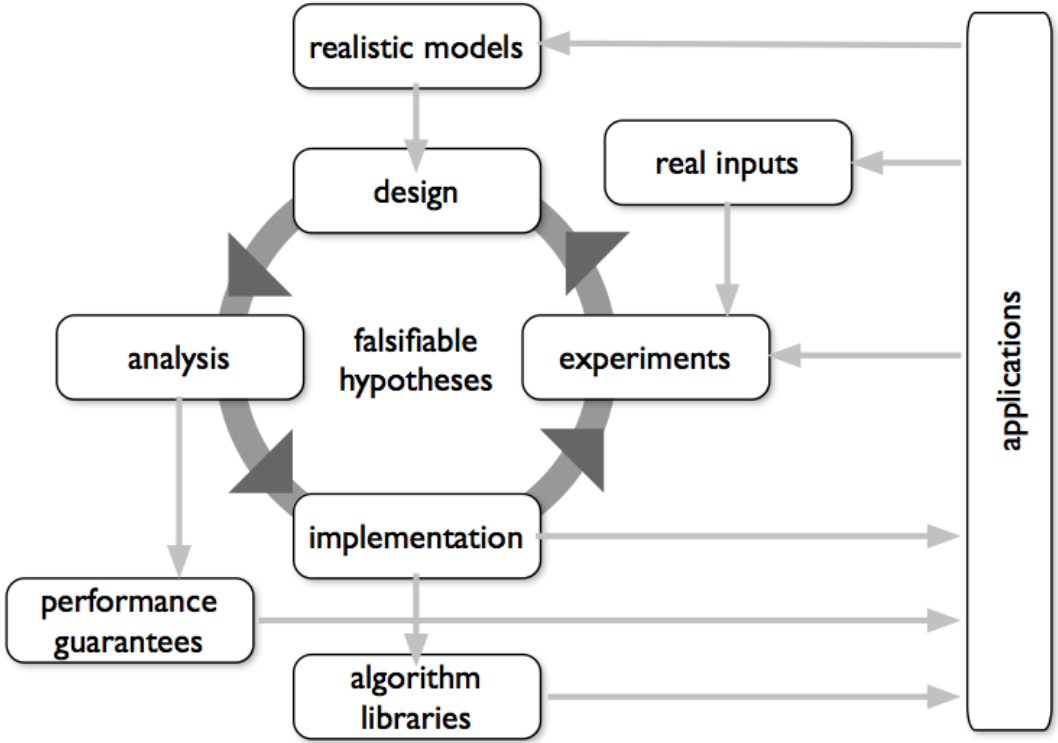
\includegraphics[width=.65\textwidth]{sources/figures/ae.png}
\caption{Algorithm Engineering schema~\cite{DBLP:conf/birthday/Sanders09}.}
\label{fig:intro:algo-eng}
\end{figure}

\paragraph{Algorithm Engineering}
The algorithmic contributions presented in this thesis were developed following
the \emph{algorithm engineering} paradigm.
Algorithm engineering can be summarized as a feedback loop of five
iterative phases: (i) modeling the problem, which usually stems from
practical applications, (ii) designing an algorithm, (iii)
analyzing it theoretically, (iv) implementing it, and (v) evaluating it
via systematic experiments (\ie experimental algorithmics), see
\Cref{fig:intro:algo-eng} for an overview.
The process is cyclic rather than sequential because experimental results
shall unveil insights about that problem that lead to further (theoretical)
improvements of the algorithms.
According to this paradigm, the implementation and the experimental evaluation
of an algorithm are not left to practitioners but are part of the whole
development process. Hence, all the algorithms presented in this thesis
are implemented in practice and evaluated on real-world instances;
in particular, they are implemented in C++ as part of the open-source
NetworKit~\cite{DBLP:journals/netsci/StaudtSM16} library.

\paragraph{Experimental Algorithmics}
As described above,
experimental evaluation is a crucial step of the algorithm engineering process.
In particular, to effectively support our conclusions, it is essential to
implement a systematic and reproducible experimental pipeline.
To this end, our experiments follow, when applicable, the guidelines for
experimental algorithmics presented in
Ref.~\cite{DBLP:journals/algorithms/AngrimanGLMNPT19} -- which I
coauthored. In particular, we carefully select appropriate sets of instances
(both real-world and synthetic) belonging
to different classes.\footnote{Although there are several ways to categorize a
network~\cite{DBLP:journals/algorithms/AngrimanGLMNPT19},
in this work, we \change{often refer to the class of \emph{complex} networks.}
As the name suggests, complex networks present non-trivial (complex)
topological features, most notably: a small diameter (\emph{small-world}
effect~\cite{newman2018networks}), clustering (\ie the tendency of vertices to
form densely connected clusters), and a skewed degree distribution
(many vertices with low degree and a few vertices with high
degree)~\cite{DBLP:journals/corr/cond-mat-0106096}.
Simple networks \change{such as road
networks or random graphs (\eg graphs generated by the \erdosr model)
do not present such features}.}
We always obtain real-world instances from public repositories (\eg
KONECT~\cite{kunegis2013konect}, SNAP~\cite{snapnets}, and others) whereas for
synthetic instances we provide details about the graph generators we used.
Also, we make our code publicly available as part of the NetworKit toolkit.
The reproducibility of our experiments is guaranteed by
managing them with SimexPal~\cite{DBLP:journals/algorithms/AngrimanGLMNPT19},
a software that automates the experimental pipeline and simplifies gathering
and analyzing the results according to the
guidelines~\cite{DBLP:journals/algorithms/AngrimanGLMNPT19}.

\section{Outline and Contribution}
%
This work is structured into five parts.
The first one provides a broad overview of the addressed network-analytic
challenges and fundamental notation and definitions,
\Crefrange{part:single-vertex-centrality}{part:matching} present in detail our
algorithmic contributions, and \Cref{part:conclusion} is devoted to concluding
remarks.
More precisely, \Cref{part:single-vertex-centrality} focuses on computing
and approximating popular single-vertex centrality measures.
In \Cref{part:group-centrality}, we consider \emph{group-centrality}, \ie the
concept of centrality extended to groups of vertices as described by
Everett and Borgatti~\cite{everett1999centrality}; in particular, we introduce
approximation algorithms and fast heuristics for group centrality maximization.
Finally, \Cref{part:matching} presents a batch-dynamic algorithm that maintains
\change{a} $\change{(1/2)}$-approximation of an MWM in fully-dynamic graphs.

The contributions presented in this thesis appeared in the publications
reported in \Cref{apx:publications}; in the following, we provide a detailed
overview.

\paragraph{\Cref{part:single-vertex-centrality}: Algorithms for Single-Vertex
Centrality Measures}
%
Centrality measures are widely used to quantify the importance of single
vertices on the basis of their structural position in a network. Concerning closeness,
Bergamini \etal~\cite{DBLP:journals/tkdd/BergaminiBCMM19} introduced an
efficient algorithm to identify the top-$k$ vertices with highest closeness
centrality that, in practice, is much faster than computing the closeness of
all vertices and extracting the top-$k$ ranking later. On dynamic graphs, however, it
would anyway be too costly to run this algorithm after each edge update (or
batch of updates). Hence, in \Cref{ch:dyn-topk}, we propose a batch-dynamic
algorithm for updating the top-$k$ ranking after multiple edge updates. Our algorithm
is developed upon the existing static strategy by Bergamini
\etal~\cite{DBLP:journals/tkdd/BergaminiBCMM19}. Experiments show that, for
single edge updates and for batches with up to $100$ edge updates, our dynamic
algorithm is one to four orders of magnitude faster than the static one.

In \Cref{ch:betweenness-approx}, we consider the problem of implementing an
effective parallelization strategy for adaptive sampling and we apply it to
betweenness centrality approximation as a case study.
%Approximation algorithms trade solution quality to reduce running time in order
%to provide solutions faster than an exact computation. In this chapter, we focus
%on \emph{adaptive sampling} algorithms.
Adaptive sampling algorithms draw random samples according to an
algorithm-specific distribution and aggregate them.
A \emph{stopping condition} determines whether enough samples have been drawn --
thus the name \enquote{adaptive}. Because the stopping condition requires to
evaluate all the data generated so far, parallelization strategies for
adaptive sampling algorithms are challenging to devise. In addition,
evaluating the stopping condition is often not cheap (\eg for our
betweenness case study, it is linear in the number of vertices of the graph);
hence, there is a trade-off between (i) frequently checking the stopping condition,
which implies additional time overhead (but avoids drawing many samples in
excess) and (ii) checking the stopping condition less frequently (with a
higher risk of drawing many samples in excess).
We introduce a new epoch-based parallelization framework for adaptive sampling
that avoids expensive synchronization costs. The main idea is to split the
execution of each thread into discrete \emph{epochs}. During an epoch, each
thread draws samples; the stopping condition is checked only at the end of
each epoch and always by the same thread, while the others keep drawing samples
for the next epoch. In this way, threads do not idle while the stopping
condition is being checked.
We adapt this framework to \kadabra, the state-of-the-art algorithm for
betweenness approximation. Our interest in \kadabra stems from the fact that
this algorithm implements an adaptive sampling technique but it fails to scale
to large numbers of threads due to high synchronization costs. We propose three
algorithms that achieve different trade-offs in terms of memory footprint and
determinism of the results. Furthermore, we use parameter
tuning~\cite{DBLP:journals/algorithms/AngrimanGLMNPT19} to optimize the
frequency of checking the stopping condition.
Our experimental study shows that our framework achieves much better parallel
speedups compared to a straightforward OpenMP-based parallelization strategy
for \kadabra.

Finally, \Cref{ch:electrical-closeness} targets the problem of approximating
\emph{electrical} centrality measures, especially electrical closeness and
forest closeness. These measures interpret the underlying graph as an
electrical network (with edge weights representing the resistance between
two vertices) and the distance between two vertices $u$ and $v$ is
computed as the resulting resistance between them (\ie the \emph{effective
resistance} or resistance distance, see \Cref{sec:prelim-resistance-distance}).
Resistance distance \change{and forest distance} consider \emph{all} the paths
between $u$ and $v$, not only the shortest ones.
%
Unfortunately, existing methods to compute electrical closeness and forest
closeness exactly rely on computing the pseudoinverse \Linv of the Laplacian
matrix \Lapl (see \Cref{sec:prelim-graphs}), which is prohibitive in terms of
both time and memory -- typically, \Linv is dense.
We present a new efficient sampling-based strategy that only requires a linear
amount of additional memory and exploits two main properties:
(i) the resistance distance between any two vertices only requires an arbitrary
column and the diagonal of \Linv (not the whole matrix) and (ii) the resistance
distance of an edge $e$ is proportional
to the fraction of the spanning trees that contain $e$. Our algorithm
provides a probabilistic $\pm\epsilon$-approximation of
\diag{\Linv} by solving just one Laplacian system
and by sampling a fixed amount of uniform spanning trees.
Experimental results show that, compared to state-of-the-art strategies,
our algorithm not only is much faster and more memory-efficient, but also
yields much more accurate approximation of \diag{\Linv} in terms of absolute
error, which results in more precise complete rankings of the elements
of \diag{\Linv}.


\paragraph{\Cref{part:group-centrality}: Algorithms for Group Centrality Measures}
%
Group centrality is useful for applications seeking sets of vertices that are
central \emph{as a group} rather than the top most individually central
vertices. Examples include finding the $k$ most influential actors in a social
network to promote some product or idea~\cite{DBLP:journals/toc/KempeKT15} or
placing resources among $k$ peers in a large P2P network so that they are
easily accessible by others~\cite{DBLP:journals/pe/GkantsidisMS06}.

Unfortunately, finding the most central group of $k$ vertices is an \np-hard
problem for most group centrality measures. This leaves approximation
algorithms and heuristics the only viable options for instances with more than
a few thousand vertices. Yet, existing algorithms for group centrality
maximization have limitations: (i) they fail to scale to large networks and, in
the group-closeness case, (ii) they do not provide any approximation guarantee.
Moreover, existing measures are not suitable for disconnected graphs. In this
part, we propose solutions to these issues.

In \Cref{ch:group-closeness-local-search,ch:ged-walk}, we target the lack of truly
scalable algorithms for group centrality maximization from two different
directions.
More precisely, \Cref{ch:group-closeness-local-search} focuses exclusively on
group-closeness: The fastest existing algorithm for this problem is the greedy
ascent heuristic by Bergamini \etal~\cite{DBLP:conf/alenex/BergaminiGM18}, which needs
several hours to handle graphs with hundreds of millions of edges.
We introduce a family of novel local search heuristics that require no more
than a few minutes to handle even larger graphs while yielding solutions with
nearly the same quality.
The fact that group-closeness is based on shortest paths poses
complexity-theoretic limitations to the development of scalable approximation
algorithms to maximize this measure. This motivates us to approach this problem
from a different angle, that is, introducing an alternative measure.
\Cref{ch:ged-walk} introduces GED-Walk (for \emph{Group Exponentially Decaying
Walk}), a novel group centrality measure inspired by Katz centrality. Similarly
to Katz, it takes into account \emph{walks} of any length -- with shorter walks
being more relevant than longer ones.
We present algorithms to compute and maximize (in approximation) GED-Walk.
On real-world networks and for groups with up to 100 vertices, our maximization
algorithm for GED-Walk is up to two orders of magnitude faster than state-of-the-art
\change{greedy} maximization algorithms for group-betweenness,
\change{group-closeness, and group-harmonic}.
%
\Cref{ch:ged-walk} also targets the lack of electrical
group centrality measures for disconnected graphs by introducing
group forest closeness, \ie forest
closeness\footnote{Forest closeness (see \Cref{sec:centrality-measures})
is an electrical centrality measure designed to handle disconnected graphs.}
extended to sets of vertices, and by adapting the greedy maximization algorithm
by Li \etal~\cite{DBLP:conf/www/0002PSYZ19} to group forest closeness.
Our experiments also show that, in connected graphs, the precision of
popular graph mining applications can be improved by GED-Walk to a greater
extent compared to other measures.
Analogous results are achieved in disconnected graphs by group forest closeness.

\Cref{ch:group-harm-clos-max} deals with approximating
group-closeness maximization. Building on top of the theoretical results
achieved in Ref.~\cite{DBLP:conf/alenex/AngrimanBDGGM21}, we present
the first approximation algorithm for this problem.
%In this chapter, we also address the issue of group centrality in disconnected
%graphs: we introduce group-harmonic closeness, \ie harmonic
%closeness\footnote{Harmonic closeness (see \Cref{sec:centrality-measures})
%handles disconnected graphs out of the box as it considers the harmonic sum
%of the distances from a vertex (or a set of vertices) to the others.}
%extended to groups of vertices, as well as a greedy approximation algorithm
%to maximize group-harmonic.
A clear trade-off between solution quality and running time emerges from our
experiments: our approximation algorithms consistently find higher quality
solutions compared to existing approaches at the cost of additional running
time.

\paragraph{\Cref{part:matching}: Maximum Weighted Matching in Fully-Dynamic Graphs}
%
On dynamic graphs, updating a previously computed matching after each
update (or a batch of updates) is a more efficient approach than
re-running a static algorithm from scratch -- similarly to what we observe in
\Cref{ch:dyn-topk} for the top-$k$ closeness centrality ranking.
%
Despite the wide range of algorithms for dynamic maximum (weighted) matching
proposed in the literature, little effort was invested into implementing these
algorithms in practice and evaluating their performance on real-world
instances. Only recently, implementations and experimental analyses were
done by Henzinger \etal~\cite{DBLP:conf/esa/Henzinger0P020} for dynamic maximum
cardinality matching algorithms and in
Ref.~\cite{conf/acda/AngrimanMSU21} for dynamic MWM -- which I coauthored.
These algorithms efficiently update an approximate maximum (weighted) matching
after single edge updates.

In \Cref{ch:dyn-mwm}, we consider the problem of maintaining a
$\change{(1/2)}$-approximate MWM after \emph{multiple} edge updates, as applications
dealing with rapidly-evolving networks may not require to compute a solution for
every single snapshot of the graph -- \eg self-organizing LTE
networks~\cite{DBLP:journals/cm/HuZZYW10}.
We take inspiration from the state-of-the-art \suitor algorithm by
Manne and Halappanavar~\cite{DBLP:conf/ipps/ManneH14}.
Our dynamic strategy is \change{conceptually} similar to the one implemented for
top-$k$ closeness in \Cref{ch:dyn-topk}: we use \suitor to compute an approximate MWM
on an initial snapshot of the graph; then, after one or multiple edge updates,
we identify the affected vertices (\ie the ones whose matching partner
needs to be updated) and update their matching partner accordingly.
Although in a worst-case scenario every vertex is affected by a single update
(which implies that our dynamic algorithm has the same \change{worst-case}
time complexity than the static \suitor), in our experiments, we see that the
actual number of affected vertices is very small -- it grows at most linearly
with the batch size. For single edge updates, our dynamic approach is on
average faster \change{than} the state of the
art~\cite{conf/acda/AngrimanMSU21}\change{,} whereas for batches with up to
$10^4$ edge updates it is two to six orders of magnitude faster than a static
recomputation (Ref.~\cite{conf/acda/AngrimanMSU21} only supports single edge
updates).

%%%%%%%%%%%%%%%%%%%%%%%%%%%%%%%%%%%%%%%%%%%%%%%%%%%%%%%%%%%%%%%%%%%%%%%%
\chapter{Preliminaries}
%%%%%%%%%%%%%%%%%%%%%%%%%%%%%%%%%%%%%%%%%%%%%%%%%%%%%%%%%%%%%%%%%%%%%%%%

\section{Graphs}
\label{sec:prelim-graphs}
% Define graphs (weights and edge directions).
% Neighbors, out/in-neighbors, degree
% Graph and network (network mainly for real scenarios e.g., social, citation, road network...)
A graph\footnote{In the literature, graphs representing real-world phenomena
are often called \enquote{networks} -- \eg social networks, road networks,
\etc We use these two names interchangeably. Further, in the context of
graphs, the names \enquote{node} and \enquote{vertex} are often used
as synonyms. We use \enquote{vertex} for an element in $V$ and we reserve
\enquote{node} for computing units in a distributed memory system.} is an ordered
pair $(V, E)$ where $V$ is the set of vertices, $E \subseteq V\times V$ is the
set of edges, $n = |V|$ is the number of vertices, and $m = |E|$ is the number
of edges.
A graph $G = (V, E)$ is a \emph{subgraph} of another graph $G' = (V', E')$ if
$G$ contains all the vertices and edges of $G'$, \ie
$V \subseteq V'$ and $E \subseteq E' \cap (V \times V)$.

An edge $e = \set{u, v} \in E$ is
\emph{incident} to $u$ and $v$ and both vertices are \emph{adjacent} to
each other.
The \emph{neighborhood} of a vertex $u$ is the set of
vertices adjacent to $u$, \ie $N(u) := \set{v \in V\ |\ \set{u, v} \in E}$. The
vertices in $N(u)$ are also called the \emph{neighbors} of $u$. The
\emph{degree} of a vertex $u$, denoted $\deg(u)$, is the cardinality of its
neighborhood.

\sloppy
If edges are ordered sets of pairs then the graph is called \emph{directed}
and we denote by $(u, v)$ an edge \emph{from} a vertex $u$ \emph{to} a vertex $v$;
otherwise, the graph is called \emph{undirected} -- \Cref{fig:undirected-graph}
and \Cref{fig:directed-graph} show an example of an undirected graph
and a directed graph, respectively.
In directed graphs, a vertex $u$ has \emph{out}-neighbors, \ie the set of
vertices $\nout(u) := \set{v\in V\ |\ (u, v) \in E}$, and \emph{in}-neighbors, \ie
$\nin(u) := \set{v\in V\ |\ (v, u) \in E}$; the neighbors of $u$ is the union of $u$'s
out-neighbors and in-neighbors: $N(u) := \nout(u) \cup \nin(u)$.
The cardinalities $\degout(u) :=
|\nout(u)|$, $\degin(u) := |\nin(u)|$, and $\deg(u) := |N(u)|$ are called
\emph{out}-degree, \emph{in}-degree, and degree of $u$, respectively.

A \emph{weighted} graph is an ordered triplet $(V, E, w)$ where $(V, E)$ is
an unweighted graph and $w$ is the \emph{weight} function, \ie $w : E
\rightarrow \real$. In weighted graphs, the degree can be extended to the sum of
the weights of the (in/out) neighbors, namely the \emph{weighted degree} and
the \emph{weighted in-} and \emph{out-degree}.
In this thesis, we only consider strictly positive edge weight functions. An
unweighted graph can also be interpreted as a weighted graph with weight
function $w : E \rightarrow 1$, \ie every edge has weight 1.

\begin{figure}[tb]
\centering
\begin{subfigure}[t]{.4\textwidth}
\centering
\begin{tikzpicture}
\vertex{-1,1}{0}{0}
\vertex{1,1}{1}{1}
\vertex{0,0}{2}{2}
\vertex{-1,-1}{3}{3}
\vertex{1,-1}{4}{4}

\edge{0}{3}
\edge{1}{2}
\edge{1}{4}
\edge{2}{3}
\edge{2}{4}
\edge{3}{4}
\end{tikzpicture}

\caption{Example of undirected graph with $n = 5$ vertices
and $m = 6$ edges.}
\label{fig:undirected-graph}
\end{subfigure}\hfill
\begin{subfigure}[t]{.4\textwidth}
\centering
\begin{tikzpicture}
\vertex{-1,1}{0}{0}
\vertex{1,1}{1}{1}
\vertex{0,0}{2}{2}
\vertex{-1,-1}{3}{3}
\vertex{1,-1}{4}{4}

\dedge{0}{3}
\dedge{1}{2}
\dbedge{1}{4}{bend left=20}
\dbedge{4}{1}{bend left=20}
\dedge{2}{3}
\dedge{2}{4}
\dedge{3}{4}
\end{tikzpicture}


\caption{Example of directed graph with $n = 5$ vertices
and $m = 7$ edges.}
\label{fig:directed-graph}
\end{subfigure}
\caption{Examples of undirected and directed graphs.}
\end{figure}

\paragraph{Matrix Representations of a Graph}
A graph $G = (V, E, w)$ can be represented using matrices. In this work,
matrices are denoted by bold capital letters such as \mat{M} and the element
at the $i$-th row and $j$-th column of \mat{M} by $\mat{M}[i, j]$. Similarly,
we type vectors as bold lowercase letters such as $\vect{v}$ and we denote the
element at index $i$ in $\vect{v}$ by $\vect{v}[i]$. The \emph{adjacency
matrix} \Adj of $G$ is a square $n \times n$ matrix such that $\Adj[u,v] = w(u,
v)$ if there is an edge from $u$ to $v$, zero otherwise. Clearly, if $G$ is
undirected, then \Adj is symmetric. The \emph{Laplacian matrix} \Lapl of $G$ is
defined as:
%
\[\Lapl := \Deg - \Adj,\]
%
where \Deg is the \emph{degree matrix} of $G$, \ie the diagonal matrix
such that $\Deg[u,u]$ is the (possibly weighted) degree of $u$.
If $G$ is undirected, then $\Lapl$ is symmetric and positive-semidefinite.
For example, the adjacency and the Laplacian matrices of the graph
in \Cref{fig:undirected-graph} are respectively:
%
\[
\Adj =
\begin{pmatrix}
0 & 0 & 0 & 1 & 0\\
0 & 0 & 1 & 0 & 1\\
0 & 1 & 0 & 1 & 1\\
1 & 0 & 1 & 0 & 1\\
0 & 1 & 1 & 1 & 0\\
\end{pmatrix}\hspace{5mm}
\text{and}\hspace{5mm}
\Lapl =
\begin{pmatrix}
1 & 0 & 0 & -1 & 0\\
0 & 2 & -1 & 0 & -1\\
0 & -1 & 3 & -1 & -1\\
-1 & 0 & -1 & 3 & -1\\
0 & -1 & -1 & -1 & 3\\
\end{pmatrix}.
\]

%%%%%%%%%%%%%%%%%%%%%%%%%%%%%%%%%%%%%%%%%%%%%%%%%%%%%%%%%%%%%%%%%%%%%%%%
%
\section{Paths and Components}
%
\begin{definition}[Walk, Trail and Path]
A walk on a graph $G = (V, E, w)$ is an alternating sequence of vertices
$(u_0, u_1, \ldots, u_\ell)$ and edges $(e_1, e_2, \ldots, e_\ell)$
where $e_i = (u_{i - 1}, u_i) \in E$ for all $0 < i \le \ell$.
The number $\ell$ of edges in the walk is called the \emph{length} of the walk.
A \emph{trail} is a walk where all edges are distinct and a \emph{path}
is a walk with distinct vertices.
\end{definition}

\begin{definition}[Random Walk]
\label{def:random-walk}
A random walk of length $\ell$ on a graph $G = (V, E, w)$ is a walk $(u_0,
u_1, \ldots, u_\ell)$ obtained in a random fashion. Starting at vertex $u_0$,
its next vertex $u_1$ is chosen at random from $u_0$'s (out) neighbors, and so
on.
\end{definition}

Hereafter, we denote $P_{s,t}$ a path where $s = u_0$ and $t = u_\ell$.
Additionally, a \change{\emph{circuit} is a trail where $u_0 = u_\ell$ and
a \emph{cycle} is a circuit with no repeated vertices}.
If a graph does not have cycles it is called \emph{acyclic}. Directed
acyclic graphs are abbreviated with the acronym DAG.

On weighted graphs, the weight of a walk $W$ is defined as the sum of the
weights of the edges it traverses:

\[
w(W) := \sum_{i = 1}^\ell w(e_i).
\]

Clearly, if the graph is unweighted, the length and the weight of a walk
coincide.\footnote{Recall that an unweighted graph is also a weighted graph where
all edges have weight 1.}

If there exists a path from a vertex $s$ to a vertex $t$, we say that $s$
\emph{reaches} $t$ or, alternatively, that $t$ is \emph{reachable} from $s$.
Reachability is important to determine connectivity and the components in a
graph.

\begin{definition}[Connected Graph]
An undirected graph is \emph{connected} if any vertex reaches any other vertex.
\end{definition}

\begin{definition}[Connected Component]
A \emph{connected component} (or CC) of a graph $G$ is a maximal connected subgraph
$C$ of $G$, \ie no additional vertex or edge can be added to $C$ without
breaking its property of being connected.
\end{definition}

Clearly, a connected graph has only one connected component -- \eg the graph in
\Cref{fig:undirected-graph} is connected.
Moreover, we call \emph{tree} an undirected acyclic connected graph and \emph{forest}
a disjoint union of trees.

\begin{definition}[Strongly Connected Graph]
A directed graph is \emph{strongly connected} if any vertex reaches any other
vertex.
\end{definition}

\begin{definition}[Strongly Connected Component]
A \emph{strongly connected component} (or SCC) of a directed graph $G$ is a
maximal strongly connected subgraph of $G$.
\end{definition}

For example, the graph in \Cref{fig:directed-graph} has three SCCs:
$\set{\set{0}, \set{3},\set{1, 2, 4}}$. Analogously to the undirected case,
strongly connected graphs consist of only one strongly connected component.
By ignoring edge directions in directed graphs, we also have \emph{weakly connected graphs}
and \emph{weakly connected components}.

\begin{definition}[Weakly Connected Graph]
A directed graph is \emph{weakly connected} all vertices are connected to each
other by a path that ignores edge directions.
\end{definition}

\begin{definition}[Weakly Connected Component]
A \emph{weakly connected component} (or WCC) of a directed graph $G$ is a
maximal weakly connected subgraph of $G$.
\end{definition}

For example, the graph in \Cref{fig:directed-graph} is weakly connected because
it has only one weakly connected component.
%
Finally, we introduce biconnectivity, \ie the property of graphs to remain
connected after the removal of a vertex.

\begin{definition}[Biconnected Graph]
A [directed] graph is \emph{biconnected} if it remains [strongly] connected
after the removal of any one vertex.
\end{definition}

\begin{definition}[Biconnected Component]
A \emph{biconnected component} of a graph $G$ is a
maximal biconnected subgraph of $G$.
\end{definition}

Clearly, the graph in \Cref{fig:undirected-graph} is not biconnected --
the removal of vertex 3 splits the graph into two connected components --
but it has two biconnected components: $\set{\set{0, 3}, \set{1, 2, 3, 4}}$.


%%%%%%%%%%%%%%%%%%%%%%%%%%%%%%%%%%%%%%%%%%%%%%%%%%%%%%%%%%%%%%%%%%%%%%%%
%
\section{Distances in Graphs}
\label{sec:distances-in-graphs}
% Shortest-path distance
% Resistance distance
% Forest distance
In mathematics, a \emph{metric} on a set $S$ is a function $d : S \times S \rightarrow \real_{\ge 0}$
that satisfies the following axioms for all $x, y, z \in S$:
\begin{enumerate}
    \item identity of indiscernibles: $d(x, y) = 0 \iff x = y$;
    \item symmetry: $d(x, y) = d(y, x)$;
    \item triangle inequality: $d(x, y) \le d(x, z) + d(z, y)$.
\end{enumerate}

We call such a function a \emph{distance function}.
Also, we define the distance between a point $s \in S$
and a subset $P \subseteq S$ as the distance from $s$ to the nearest point in
$P$:

\begin{equation}
\label{eq:def:dist-point-set}
d(s, P) := \min_{p \in P}d(s, p).
\end{equation}

In an undirected graph $G = (V, E, w)$ with positive edge weights,
the \emph{vertex distance} is a metric $d: V\times V \rightarrow \real_{\ge 0}$
defined on all the pairs of vertices in $G$.
Notwithstanding that the symmetry property does not necessarily hold in
directed graphs, we follow the standard convention and use the term
\enquote{distance} even in the directed case.
We now introduce three vertex distance measures that are necessary for the
definition of the centrality measures described in
\Cref{sec:centrality-measures,sec:group-centrality-measures}.


%%%%%%%%%%%%%%%%%%%%%%%%%%%%%%%%%%%%%%%%%%%%%%%%%%%%%%%%%%%%%%%%%%%%%%%%
%
\subsection{Shortest-path Distance}
%
The shortest-path distance, also known as the \emph{geodesic} distance,
is one of the most natural and common definitions of vertex distance in graphs.
The \emph{shortest path} between two vertices $s$ and $t$ is the path $P_{s,t}$
with minimum weight -- note that such a path might not be unique.

\begin{definition}[Shortest-path Distance]
The \emph{shortest-path distance} is the function
$d : V \times V \rightarrow \real_{\ge 0}$ such that $d(s, t)$
is the weight of the path $P_{s,t}$ with minimum weight.
\end{definition}

Conventionally, if $t$ is not reachable from $s$, the distance $d(s, t)$ is
defined as infinite.

\begin{definition}[Diameter]
The \emph{diameter} of a graph of a graph $G$ is the maximum
shortest-path distance between two reachable vertices $u$ and $v$ where $u$
reaches $v$:
%
\[\diam(G) := \max_{\substack{u,v\in V,\\d(u, v) < +\infty}}d(u, v).\]
\end{definition}

\begin{definition}[Eccentricity]
The \emph{eccentricity} of a vertex $u \in V$ is the maximum shortest-path
distance from $u$ to a vertex $v$ reachable from $u$:
\[\ecc(u) := \max_{\substack{v\in V,\\d(u, v) < +\infty}} d(u, v).\]
\end{definition}


Computing the shortest path between two vertices is a classic problem in
algorithmic graph theory and can be solved by the well-known Dijkstra's
algorithm in $\Oh(m + n\log n)$ time -- if the priority queue is implemented
using a Fibonacci Heap.
The same algorithm can also solve the more general \emph{Single-Source Shortest Path}
problem (or SSSP), \ie finding the shortest distances from a vertex to \emph{all}
the other vertices in a graph, in $\Theta(m + n\log n)$ time. If the graph is
unweighted, both the shortest path and the SSSP problems can be solved in $\Oh(n +
m)$ time with a Breadth-First Search (or BFS). The problem of computing the
shortest-path distances between all pairs of vertices is known as the
\emph{All-Pairs Shortest Path} problem (or APSP), and can be solved in $\Oh(nm +
n^2\log n)$ time by \change{running Dijkstra's algorithm from each vertex or
-- for graphs with arbitrary edge weights --} Johnson's algorithm. On
unweighted graphs, in turn, it suffices to run a BFS from each vertex, which
requires $\Theta(n^2 + nm)$ time.

In addition to the aforementioned \emph{combinatorial} techniques,
shortest-path distance problems can also be solved algebraically via
\emph{matrix multiplication}. APSP can be solved in $\Oh(n^\omega \log n)$ by
repeatedly squaring the adjacency matrix of a graph, where $\omega <
\numprint{2.373}$~\cite{DBLP:conf/soda/AlmanW21}
is the matrix multiplication exponent, \ie the smallest constant such that the
product of two $n\times n$ matrices can be performed within $\Oh(n^{\omega +
o(1)})$ algebraic operations.
The logarithmic factor of the time complexity can be saved by a recursive
decomposition of the problem~\cite[Theorem 5.7, p. 204]{DBLP:books/aw/AhoHU74}.
In case of integral edge weights, further improvements have been proposed
for undirected~\cite{DBLP:conf/focs/ShoshanZ99} and directed graphs
\cite{DBLP:conf/focs/Zwick98,DBLP:conf/stoc/Zwick99}.
Despite being asymptotically faster than combinatorial algorithms on dense
graphs,\footnote{The \emph{density} of a graph is $m / {n \choose 2}$,
\ie the fraction of edges actually present in the graph over the maximum
possible number of edges. Consider a sequence of graphs of increasing number
of vertices $n$. If the density approaches zero as $n$ becomes large, the
graphs are said to be \emph{sparse}. Otherwise, a graph where the density
remains non-zero in the limit of large $n$ is said to be
\emph{dense}. Clearly, we cannot take the limit of real-world networks and thus
we cannot determine formally whether they are sparse or dense.
Informally, however, for these networks \enquote{sparse} means that most of
the edges that could exist in the network are not present~\cite[Section
6.10.1]{newman2018networks}.}
methods based on matrix multiplication are in practice not applicable to large
graphs because they require to store dense matrices.


%%%%%%%%%%%%%%%%%%%%%%%%%%%%%%%%%%%%%%%%%%%%%%%%%%%%%%%%%%%%%%%%%%%%%%%%
%
\subsection{Resistance Distance}
\label{sec:prelim-resistance-distance}
%
In the context of determining the distance between two vertices in a graph,
some applications require to take into account not only the \emph{shortest} paths,
but \emph{all} the paths between the two
vertices~\cite{DBLP:journals/socnet/Borgatti05,
DBLP:journals/corr/abs-math-0602073,stephenson1989rethinking}.
A typical example are
electrical networks: an electrical network can be
regarded as an undirected weighted graph $G = (V, E, r)$ where
edges are \emph{resistors} and $r : E \to \real_{> 0}$ is the
\emph{resistance} of an edge. The \emph{conductance} of an edge $e$
is defined as the reciprocal its resistance: $c(e) = 1/r(e)$.
Let $e = \set{a, b}\in E$ and let $p(a,b) = p(a) - p(b)$ be the
electric \emph{potential difference} between $a$ and $b$; then, according to
Ohm's law, an amount
%
\[i(a,b) = \frac{p(a,b)}{r(e)}\]
%
of \emph{electrical current} flows from $a$ to $b$.
Notice that, although the graph is undirected,  the electrical current has a
\emph{direction} which is determined by the sign of potential difference, and thus
$p(a,b) = -p(b,a)$ and $i(a,b) = -i(b,a)$. The current always flows from
the vertex with the highest potential to the vertex with the lowest potential.
Potential differences and currents in an electrical network are governed by the
two well-known Kirchhoff's potential and current
laws~\cite{DBLP:books/daglib/0009415,DBLP:conf/lcn/LuoWCC05}.

\simpletheorem{kirchpot}{Kirchhoff's potential law}{The potential differences
round any cycle $(u_1, u_2, \ldots, u_\ell)$ sum to zero:
%
\[p(u_1, u_2) + p(u_2, u_3) + \ldots + p(u_\ell, u_1) = 0.\]}

\simpletheorem{kirchcur}{Kirchhoff's current law}{The total current outflow
from any vertex $u$ is zero:
%
\[i(u, \infty) + \sum_{v \in N(u)} i(u, v) = 0.\]
%
Here $i(u, \infty)$ denotes the amount of current leaving  the network at
vertex $u$ -- in accordance with our notation, $i(\infty, u) = -i(u,
\infty)$ is the amount of current entering the network at vertex $u$.}

In most problems, current enters the network at some vertices
and leaves it at others. Such a general problem can be reduced to the
fundamental problem where a unit of current enters the network at a
vertex $s$, called the \emph{source}, and leaves it at another vertex $t$,
called the \emph{sink}.

The \emph{effective conductance} from $s$ to $t$, $\ceff(s, t)$, is the
amount of current flowing from $s$ to $t$ when $p(s,t) = 1$.
The \emph{effective resistance} $\reff(s,t) = 1/\ceff(s,t)$
is the potential difference between $s$ to $t$ when a unit of current flows
from $s$ to $t$~\cite[Ch. IX]{DBLP:books/daglib/0009415}.
This quantity is also referred to as the \emph{resistance
distance} between $s$ and $t$~\cite{DBLP:journals/siamrev/GhoshBS08}.

\begin{definition}[Resistance Distance]
\label{def:resistance-distance}
Let $G = (V, E, r)$ be a graph. The resistance distance (or
effective resistance) is a metric $\rdist : V \times V \to \real_{\ge 0}$
defined as the potential difference between two vertices $s$ and $t$ ensuring
$s$ as the source vertex, $t$ as the sink vertex, and a unit of current from
$s$ to $t$.
\end{definition}

Let $z\in V$ and $\cunit{z}$ be the canonical unit vector for $z$, \ie
$\mat{e}_z[u] = 0$ for all $u \neq z$ and $\cunit{z}[z] = 1$.
The resistance distance between $s$ and $t$ can be computed as follows:
%
\begin{equation}
\label{eq:eff-res-laplinv}
\rdist(s, t) = (\cunit{s} - \cunit{t})^\top\Linv(\cunit{s} - \cunit{t}) =
\Linv[s,s] - 2\Linv[s,t] + \Linv[t,t],
\end{equation}
%
where \Linv is the Moore-Penrose pseudoinverse of the Laplacian
matrix~\cite[p. 290]{DBLP:books/daglib/0086372}.
\Linv can be expressed as~\cite{van2017pseudoinverse}:
%
\begin{equation}
\label{eq:laplinv}
\Linv = \roundb{\Lapl + \frac1n \Ones}^{-1} - \frac1n \Ones,
\end{equation}
%
where $\Ones$ is the $n \times n$-matrix with all elements equal to one.
$\Linv$ has numerous applications in physics and engineering~\cite{van2017pseudoinverse}
as well as applied mathematics~\cite{DBLP:books/daglib/0086372}
and graph (resp. matrix) algorithms~\cite{DBLP:conf/www/0002PSYZ19}.
A straightforward way to compute the resistance distance between two
vertices is to compute \Linv. However, this approach is limited to small graphs
because it requires $\Oh(n^3)$ time and $\Oh(n^2)$ memory as \Linv is generally
a dense matrix.
Clearly, to compute $\rdist(s, t)$, only three elements of \Linv are needed, and
selected elements of \Linv can be computed in practice more efficiently than
computing the whole
\Linv~\cite{DBLP:journals/pc/Jacquelin0018,DBLP:journals/toms/LinYMLYE11}.

The resistance distance between
two vertices $u$ and $v$ is proportional to the
\emph{commute time} between $u$ and $v$, namely:
%
\[\ct(u, v) := \hitt(u, v) + \hitt(v, u) = \vol(G)\cdot\reff(u, v),\]
%
where $\hitt(u, v)$ is the \emph{hitting time} from $u$ to $v$, \ie the
expected length of a random walk (see \Cref{def:random-walk}) that starts in
$u$ and ends in $v$, and $\vol(G)$ is the \emph{volume} of $G$, \ie the sum of
the edge weights of the graph. The commute time can be interpreted as the
expected length of a random walk for going from $u$ to $v$ and back to $u$
again~\cite{DBLP:conf/stacs/BrandesF05}.

%%%%%%%%%%%%%%%%%%%%%%%%%%%%%%%%%%%%%%%%%%%%%%%%%%%%%%%%%%%%%%%%%%%%%%%%
%
\subsection{Forest Distance}
\label{sec:prelim:forest-distance}
%
Forest distance is a one-parametric family of metrics introduced by Chebotarev
and Shamis~\cite{chebotarev2000forest,DBLP:journals/endm/ChebotarevS02}
that takes into account all the paths between two vertices.
Contrary to resistance distance, forest distance (i) applies to disconnected
graphs out of the box\footnote{Resistance distance requires some adjustments to
handle disconnected graphs.}
and (ii) allows to control the influence of the length of
the paths between the two vertices over the value of their distance via a
parameter $\alpha > 0$.
Forest distances have been shown to effectively capture sensitive relationship
indices such as social proximity and group cohesion and thus has found
application in sociology~\cite{DBLP:journals/corr/abs-math-0602070}.

\begin{definition}[Rooted Spanning Forest]
Let $G = (V, E, w)$ be an undirected graph with $c$ connected components $(C_1,
C_2, \ldots, C_c)$ and let $T_i$ be a spanning tree of the component $C_i$.
A \emph{spanning forest} on $G$ is the disjoint union $\cup_{i = 1}^c T_i$. A
spanning forest is \emph{rooted} if each spanning tree $T_i$ has a vertex
marked as its root.
\end{definition}

Let $G = (V, E, w)$ be an undirected graph and let $\alpha > 0$.
The forest distance is defined in terms of the parametric \emph{forest matrix}
of $G$, \ie
\begin{equation}
\label{eq:forest-matrix}
\Fmatp := \roundb{\Ident + \alpha\Lapl}^{-1}.
\end{equation}

The name \emph{forest} stems from the fact that
the element $\Fmatp[u, v]$ is the fraction of rooted spanning forests
where $u$ is the root of a tree and $v$ belongs to the same
tree~\cite{chebotarev2000forest,DBLP:conf/icdm/JinBZ19}.
%
An alternative definition of the forest matrix preferred in other
works such as Ref.~\cite{DBLP:journals/corr/abs-math-0602073} is $(\alpha\Ident +
\Lapl)^{-1}$, which is equivalent to the one given in \Cref{eq:forest-matrix}
up to a scaling factor of the edge weights of the graph.
%
The forest matrix $\Fmatp$ is symmetric and doubly
stochastic~\cite{merris1997doubly}, \ie for all $i,j\in\set{1,\ldots,n}$:
%
\[
\Fmatp[i, j] \ge 0,\hspace{5mm}\ones^\top\Fmatp = \ones^\top,\hspace{5mm}\Fmatp\ones = \ones,
\]
%
where \ones is the all-ones vector. Further, $\Fmatp[i,j]$ is $0$ iff $i$ and
$j$ are in two different components, whereas $\Fmatp[i,i] \le 1$ with equality
iff $i$ is an isolated vertex~\cite{merris1998doubly}.

\begin{definition}[Forest Distance~\cite{chebotarev2000forest}]
\label{def:forest-distance}
Let $G = (V, E, w)$ be an undirected graph, $\alpha > 0$, and $s,t\in V$. The
forest distance is a one-parametric metric $\fdistp : V \times V \to \real_{\ge 0}$
defined as:
%
\[
\fdistp(s, t) := (\cunit{s} - \cunit{t})^\top \Fmatp (\cunit{s} - \cunit{t}) =
\Fmatp[s,s] - 2\Fmatp[s,t] + \Fmatp[t,t].
\]
\end{definition}

Higher values of $\alpha$ give greater importance to long paths. To see this we
analyze the asymptotic behavior of $\fdistp(s, t)$ with respect to $\alpha$. As
$\alpha \to 0$, $\fdistp(s, t)$ tends to the discrete metric:
%
\[
\fdist_0(s, t) =
\begin{cases}
0 &\text{if}\ s = t\\
1 &\text{otherwise}.
\end{cases}
\]

Let us denote by $V_s$ the set of vertices in the connected component that contains
vertex $s$. As $\alpha \to \infty$, $\fdistp(s, t)$ tends
to~\cite{chebotarev2000forest}:
%
\[
\fdist_{\infty}(s, t) =
\begin{cases}
0 & \text{if}\ t \in V_s\\
\frac 12 \roundb{\frac{1}{|V_s|} + \frac{1}{|V_t|}} & \text{otherwise}.
\end{cases}
\]

%%%%%%%%%%%%%%%%%%%%%%%%%%%%%%%%%%%%%%%%%%%%%%%%%%%%%%%%%%%%%%%%%%%%%%%%
%
\section{Centrality Measures}
\label{sec:centrality-measures}
% Degree, Betweenness, Closeness, Harmonic, Electrical closeness, Forest closeness,
% ED-Walk

Given a graph $G = (V, E, w)$, a \emph{centrality measure} is a function $c : V \to
\real$ that assigns a \emph{centrality score} to
each vertex depending on its structural position in the graph. The main
intuition is that, if a vertex has a central position in the graph (\ie it is
\emph{structurally central}), then it is also important or has some degree of
influence in the network under consideration.
Clearly, what makes a vertex central in a network is highly application-dependent,
and thus a universal definition of centrality cannot be given.
Over the past decades, numerous centrality measures were introduced and applied
in a multitude of contexts and
applications~\cite{cohn1958networks,pitts1965graph,action1993rise,
mackenzie1966structural,beauchamp1965improved,singh2022}.
%
In this section, we describe the centrality measures that are relevant to our
contributions, for a broader survey
see~\parencites[][Ch.~7.1]{DBLP:journals/socnet/Borgatti05,newman2018networks,
DBLP:journals/it/GrintenAM20}.
%
As in~\cite{DBLP:journals/im/BoldiV14}, we categorize centrality measures into
three main classes: \emph{distance-based} measures,
\emph{spectral} measures and \emph{path-based} measures.
%
For the sake of comparison, in the heatmaps in
\Cref{fig:karate-centrality}, we exemplify the centrality of the members of
the popular Zachary's karate club social network~\cite{zachary1977information}
according to different centrality measures.


\begin{figure}[t!]
\centering
\begin{subfigure}[t]{.45\textwidth}
\centering
\includesvg[width=\textwidth]{karate-degree}
\caption{Degree centrality}
\label{fig:karate-degree}
\end{subfigure}\hfill
%
\begin{subfigure}[t]{.45\textwidth}
\centering
\includesvg[width=\textwidth]{karate-betweenness}
\caption{Betweenness centrality}
\label{fig:karate-betw}
\end{subfigure}\smallskip

\begin{subfigure}[t]{.45\textwidth}
\centering
\includesvg[width=\textwidth]{karate-closeness}
\caption{Closeness centrality}
\label{fig:karate-clos}
\end{subfigure}\hfill
%
\begin{subfigure}[t]{.45\textwidth}
\centering
\includesvg[width=\textwidth]{karate-harmonic}
\caption{Harmonic centrality}
\label{fig:karate-harmonic}
\end{subfigure}\smallskip

\begin{subfigure}[t]{.45\textwidth}
\centering
\includesvg[width=\textwidth]{karate-electrical-clos}
\caption{Electrical closeness centrality}
\end{subfigure}\hfill
%
\begin{subfigure}[t]{.45\textwidth}
\centering
\includesvg[width=\textwidth]{karate-forest-clos}
\caption{Forest closeness centrality}
\end{subfigure}\smallskip

\begin{subfigure}[t]{.45\textwidth}
\centering
\includesvg[width=\textwidth]{karate-eigenvector}
\caption{Eigenvector centrality}
\end{subfigure}\hfill
%
\begin{subfigure}[t]{.45\textwidth}
\centering
\includesvg[width=\textwidth]{karate-katz}
\caption{Katz centrality}
\end{subfigure}\smallskip

\begin{subfigure}[t]{.45\textwidth}
\centering
\includesvg[width=\textwidth]{karate-pagerank}
\caption{PageRank}
\end{subfigure}

\caption{Heatmaps of vertex centrality scores of the vertices in the
Zachary's karate club social network~\cite{zachary1977information}.
Red means high centrality score, blue means low centrality score. Images were
generated with the Gephi software~\cite{DBLP:conf/icwsm/BastianHJ09}.}
\label{fig:karate-centrality}
\end{figure}

\subsection{Distance-based Measures}
\label{sec:prelim-dist-based-centrality}
%
Distance-based centrality measures express the importance of a vertex $u$ as a
function of a distance metric between $u$ and other vertices (see
\Cref{sec:distances-in-graphs}).
The distance to other vertices is one of the most natural ways to assess the
importance of a vertex in a network, and therefore these measures are among
the first ever defined.

\paragraph{Degree Centrality}
%
The degree of a vertex is probably the simplest and oldest centrality
measure ever used~\cite{freeman1978centrality}. Even though it only takes
into account the immediate neighbors of a vertex,
degree centrality has been shown to be strongly correlated with other centrality
measures such as closeness, betweenness, and eigenvector
centrality in real-world networks~\cite{valente2008correlated, lim2011online}.
This is also clear from the example in \Cref{fig:karate-centrality}: the
vertices with highest degree (see \Cref{fig:karate-degree}) are also central
according to other measures.


\paragraph{Closeness Centrality}
%
Recall from \Cref{sec:intro:context} that closeness was introduced in 1950 by
Bavelas in his attempt of capturing how a communication pattern may affect the
performance of a group of people~\cite{bavelas1950communication}. A vertex in a
network is considered \emph{central} if the sum of the geodesic distances to
all the other vertices is low. Intuitively, the time required by a message to
be spread throughout an entire network is minimized if the message originates
from the most central vertex.

Such a definition of closeness depends upon the number of vertices
in the network from which it is calculated, and therefore comparing the closeness
of vertices in networks with different sizes would be meaningless.
Beauchamp~\cite{beauchamp1965improved} solved this issue by suggesting
a normalization factor for closeness of $n-1$.
The closeness centrality of a vertex $u$ is thus defined as:

\begin{equation}
\label{eq:def:closeness}
\clos(u) := \frac{n - 1}{\sum_{v \in V} d(u, v)}.
\end{equation}

The denominator is also known as the \emph{farness} of $u$, or $f(u)$.
Closeness centrality may also be interpreted as the reciprocal of the average
distance from $u$ to the other vertices.
%
Notice that $\clos(\cdot)$ is only defined on (strongly) connected graphs -- if
some vertex $u$ cannot reach some other vertex $v$, then $d(u, v)$ is infinity.
To overcome this limitation, Lin introduced Lin's
index~\cite{lin1976foundations}:
%
\[c_{\text{Lin}}(u) := \frac{r^2(u)}{\sum_{v \in R(u)}d(u, v)},\]
%
where $R(u)$ is the set of vertices reachable from $u$ and $r(u)$ is $|R(u)|$.
Olsen \etal~\cite{DBLP:conf/icde/OlsenLH14} proposed a further definition of
closeness for disconnected graphs:
%
\[\clos(u) := \frac{\roundb{r(u) - 1}^2}{(n - 1) \sum_{v \in R(u)} d(u, v)}.\]
%

Unless stated differently, hereafter we refer to the definition in
\cref{eq:def:closeness}, which is well-established in the
literature~\cite{DBLP:journals/im/BoldiV14}.

Apart from requiring some adjustments to handle disconnected graphs,
another known weakness of closeness centrality is its limited capability to
discriminate different vertices, especially on complex networks. A typical
characteristic of complex networks is having a small
diameter~\cite{DBLP:journals/corr/cond-mat-9907038}. Hence, all distances --
and thus all closeness values -- lie within a narrow
interval~\cite{DBLP:journals/it/GrintenAM20}. To show this in practice, we pick
$100$ vertices uniformly at random from the networks of
\Cref{tab:prelim:insts-rstd} and we compute their closeness centrality and the
shortest-path distances from those vertices to the others.
\Cref{fig:prelim:rstd} reports the mean and the relative standard deviation of
the shortest-path distances and of the closeness centrality for the networks of
\Cref{tab:prelim:insts-rstd}. The relative standard deviation
is the standard deviation ($\sigma$) divided by the mean ($\mu$) and shows
the extent of variability with respect to the mean of the distribution.
For example, for the \enquote{advogato} network, the standard deviation is
$\advogatoccrstd$ of the mean $\mu = \advogatoccmean$, which is quite
low.\footnote{In this example, $\sigma = \advogatoccstd$ which means that,
assuming a normal distribution of the closeness scores, $\approx 68\%$ of
the values of $\clos(\cdot)$ are in the interval $[\advogatoonesigmabegin,
\advogatoonesigmaend]$ while $\approx 95\%$ of the values are in
$[\advogatotwosigmabegin, \advogatotwosigmaend]$.}
%
Such limitation can also be observed from \Cref{fig:karate-clos}: compared
to other measures (\eg betweenness or PageRank), closeness fails in discriminating
highly-central vertices from the others -- as several vertices have a high
or very similar centrality score.

\begin{figure}[t!]
\centering
\begin{minipage}[t]{.5\textwidth}
\centering
\begin{figure}[H]
\centering
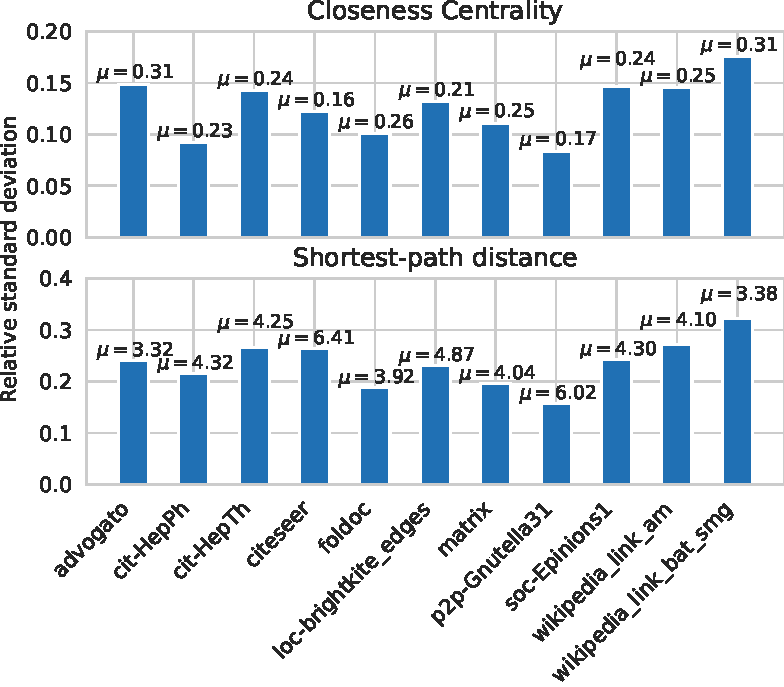
\includegraphics[width=.9\textwidth]{sources/plots/preliminaries/sp-cc-rstd.pdf}
\caption{Relative standard deviation for shortest-paths distances and for
closeness centrality for the networks in \Cref{tab:prelim:insts-rstd}.}
\label{fig:prelim:rstd}
\end{figure}
\end{minipage}\hfill
\begin{minipage}[t]{.5\textwidth}
\centering
\begin{table}[H]
\centering
\setlength{\tabcolsep}{3pt}
\scriptsize
\begin{tabular}{lrrr}
\toprule
Network & $n$ & $m$ & Diameter\\
\midrule
advogato & \numprint{5042} & \numprint{52195} & \numprint{9}\\
cit-HepPh & \numprint{34401} & \numprint{421529} & \numprint{14}\\
cit-HepTh & \numprint{27400} & \numprint{352580} & \numprint{15}\\
citeseer & \numprint{365154} & \numprint{1742596} & \numprint{34}\\
foldoc & \numprint{13356} & \numprint{120238} & \numprint{8}\\
loc-brightkite\_edges & \numprint{56739} & \numprint{212945} & \numprint{18}\\
matrix & \numprint{79116} & \numprint{515397} & \numprint{12}\\
p2p-Gnutella31 & \numprint{62561} & \numprint{147878} & \numprint{11}\\
soc-Epinions1 & \numprint{75877} & \numprint{508836} & \numprint{15}\\
wikipedia\_link\_am & \numprint{20883} & \numprint{105714} & \numprint{12}\\
wikipedia\_link\_bat\_smg & \numprint{21814} & \numprint{123756} & \numprint{13}\\
\bottomrule
\end{tabular}
\caption{Graphs used in \Cref{fig:prelim:rstd} (downloaded from
the public repository KONECT~\cite{kunegis2013konect}).}
\label{tab:prelim:insts-rstd}
\end{table}
\end{minipage}
\end{figure}

\paragraph{Harmonic Centrality}
%
Marchiori and Latora~\cite{marchiori2000harmony} introduced the
\emph{connectivity length} of a graph in order to measure the \emph{efficiency}
of a network in terms of information propagation. The connectivity length of a
graph is defined as the \emph{harmonic mean} of all the pairwise distances
between the vertices in a graph.
Later, harmonic centrality was independently devised by
Dekker~\cite{DBLP:journals/joss/Dekker05} (with the name \enquote{valued
centrality}) and by Rochat~\cite{rochat2009closeness}.
Harmonic centrality is defined as:

\begin{equation}
\label{eq:def:harmonic}
\harm(u) := \sum_{v \in V \setminus \set{u}} \frac{1}{d(u, v)}.
\end{equation}

Under the reasonable assumption that the reciprocal of infinity is zero,
harmonic centrality is well-defined also on disconnected graphs.
%
Further, from an axiomatic point of view, harmonic centrality enjoys several
desirable properties~\cite{DBLP:journals/im/BoldiV14}.


\paragraph{Electrical Closeness}
Electrical closeness~\cite{DBLP:conf/stacs/BrandesF05} --
also known as \emph{current-flow closeness} or \emph{information
centrality}~\cite{stephenson1989rethinking} --
ranks vertices according to their average resistance distance
to the others:
%
\begin{equation}
\label{eq:electrical-closeness}
\elclos(u) := \frac{n - 1}{\sum_{v \in V\change{\setminus\set{u}}} \rdist(u, v)}.
\end{equation}

Analogously to combinatorial closeness, electrical closeness is not directly
applicable to disconnected graphs due to the aforementioned infinite distances
issue. However, generalizations to disconnected graphs such as
Lin's~\cite{lin1976foundations} or Olsen's~\cite{DBLP:conf/icde/OlsenLH14}
apply as well.

Because it takes into considerations all the paths between two vertices,
electrical closeness solves two issues concerning the vertex rankings computed by
combinatorial closeness: (i) having a low discriminative power,
especially on complex networks, and (ii) being
highly susceptible to changes in the graph~\cite{DBLP:journals/it/GrintenAM20}.
These claims are corroborated by the experiments in
Ref.~\cite{DBLP:conf/siamcsc/BergaminiWLM16}.


\paragraph{Forest Closeness}
%
Forest distance closeness centrality (abbreviated with \emph{forest closeness})
is a further variation of closeness centrality where the shortest-path distance
is replaced by the \emph{forest distance}:
%
\begin{equation}
\label{eq:forest-closeness}
\fclosp(u) := \frac{n}{\sum_{v \in V \setminus \set{u}}{\fdistp(u, v)}}.
\end{equation}

The denominator of $\fclosp(u)$ is also called the \emph{forest farness} of $u$.
Compared to other centrality measures, forest closeness presents two main advantages:
(i) by taking all paths into account it has a high discriminative
power~\cite{DBLP:conf/icdm/JinBZ19} and (ii) it handles disconnected
graphs out of the box.

\subsection{Spectral Centrality Measures}
%
\emph{Spectral centrality measures} compute the importance of the vertices of a
graph $G$ by using the left dominant eigenvector of a matrix derived
from a matrix representation of $G$.
The existence and the uniqueness of most of these measures is guaranteed by the
theory developed by Perron and
Frobenius~\cite{perron1907theorie,frobenius1912matrizen} about non-negative
matrices~\cite{DBLP:books/siam/BermanP94}.

\paragraph{Eigenvector Centrality}
Eigenvector centrality implements the idea that a vertex in a network is
important if adjacent to vertices that are themselves important. It can also be
interpreted as an extension of degree centrality where the centrality of a
vertex is \emph{proportional to the centrality of its neighbors}.

Let $\lambda$ be the dominant eigenvalue of the adjacency matrix \Adj of a
graph. Assuming that $V = \set{1, \ldots, n}$, \ie all vertices
in $G$ are indexed from 1 to $n$, the eigenvector centrality
of a vertex $u \in V$ is defined as:
%
\begin{equation}
\label{eq:prelim:eig-centrality}
\eig(u) = \frac 1\lambda\sum_{v = 1}^n A[u,v]\cdot\eig(v),
\end{equation}

In matrix notation, \Cref{eq:prelim:eig-centrality} is equivalent
to $\eig(u) = \vect{x}[u]$ where \vect{x} is the right leading eigenvector
that solves the linear system
$\Adj\vect{x} = \lambda\vect{x}$.

If \Adj is irreducible,\footnote{
A square matrix \mat{M} is called \emph{reducible} if there exists a
permutation matrix \mat{P} such that:
%
\[
\mat{PMP}^{-1} =
\begin{pmatrix}
    \mat{B}_{1,1} & \mat{B}_{1,2}\\
    0 & \mat{B}_{2,2}
\end{pmatrix},
\]
%
where $\mat{B}_{1,1}$ and $\mat{B}_{2,2}$ are non-empty square matrices.
A matrix that cannot be reduced is called \emph{irreducible}.
}
%
the Perron-Frobenius theorem implies that $\lambda > 0$ and that all the
entries of $\vect{x}$ are strictly positive. \Adj is irreducible iff the
corresponding graph is strongly connected~\cite{DBLP:books/siam/BermanP94}. In
case of disconnected graphs, however, the eigenvector centrality of some
vertices could be zero~\cite{newman2018networks}, which makes this measure
suitable for (strongly) connected graphs only.

\paragraph{Katz Centrality}
%
The limitation of eigenvector centrality of being restricted to strongly
connected graphs is resolved by Katz centrality~\cite{katz1953new}. Conversely
to distance-based based centrality measures that only consider shortest paths,
this measure takes into account \emph{all the walks} between two vertices, with
shorter walks having a greater contribution to the centrality score than longer
walks.
%
The Katz centrality of a vertex $u$ is:
%
\begin{equation}
\label{eq:def:katz}
\katz(u) := \sum_{i = 1}^{\infty}\alpha^i \sum_{v\in V} \Adj^i[u, v],
\end{equation}
%
which converges if the \emph{attenuation factor} $\alpha > 0$ is less than the
reciprocal of the largest singular value of \Adj.
Eq.~\eqref{eq:def:katz} can be rewritten in matrix terms:
%
\begin{equation}
\label{eq:def:katz-alg}
\vect{c}_{\text{K}} = \roundb{\roundb{\Ident - \alpha\Adj}^{-1} - \Ident}\ones,
\end{equation}
%
where $\vect{c}_{\text{K}}[u]$ is the Katz centrality of $u\in V$.


\paragraph{PageRank}
Originally designed with the purpose of developing a search engine,
PageRank~\cite{page1999pagerank} is among the most recent and popular spectral
centrality measures.
Despite being tailored to the Internet graph, as of today this measure is used
in applications beyond web graphs~\cite{DBLP:journals/siamrev/Gleich15}.
%
PageRank models the stationary distribution of a random walk over the vertices
of a graph. At any step, the random walk jumps to another random vertex
with probability $1 - \alpha$, where $\alpha \in (0, 1)$ is called
the \emph{damping factor}. The PageRank score of a vertex $u$ is defined as:
%
\[
\pr(u) := \alpha \sum_{v \in N(u)}\frac{\pr(v)}{\deg(v)} + \frac{1 - \alpha}{n}.
\]

\subsection{Path-based Centrality Measures}
\label{sec:prelim:path-based-centrality}
%
Path-based centrality measures take into account all the (shortest) paths hitting
a vertex. Notice that, in unweighted graphs, degree centrality can also be
considered a path-based measure since it evaluates the number of incoming or
outgoing paths of length one.

\paragraph{Betweenness Centrality}
%
Freeman~\cite{freeman1977set} introduced betweenness centrality as a measure of
how much a vertex \emph{controls} the information flow in a network. A vertex
is considered central if it stands \emph{between} other vertices, as it can
control or influence their communications -- under the assumption that
information flows through shortest paths exclusively.
%
More formally, the betweenness centrality of a vertex $u$ is defined as
the probability that a shortest path between any two vertices $x,y \in V
\setminus \set{u}$ passes through $u$.
Let $\sigma_{x,y}$ be the number of shortest paths from $x$ to $y$, and
$\sigma_{x,y}(u)$ be the number of such paths that cross $u$. The betweenness
centrality of $u$ is defined as:
%
\begin{equation}
\label{eq:def:betweenness}
\betw(u) := \sum_{\substack{x,y \in V \setminus \set{u}\\x\neq y,\ \sigma_{x,y} \neq 0}}
\frac{\sigma_{x,y}(u)}{\sigma_{x,y}}.
\end{equation}

Vertices with high betweenness centrality can also be interpreted
as crucial actors whose removal from the network would disrupt most
communications between other vertices~\cite{DBLP:journals/snam/BoldiRV13}.
Indeed, in the example in \Cref{fig:karate-betw}, the removal of
the vertex with highest betweenness (the red one) would isolate six
vertices from the entire network.


\paragraph{\edw Centrality}
Inspired by Katz centrality, in Ref.~\cite{DBLP:conf/alenex/AngrimanGBZGM20}, we
define \edw, a new centrality measure designed to possess two main
properties: (i) to take into consideration \emph{all walks} (not just shortest
paths) of \emph{any length} that cross a vertex and (ii) to admit a natural
generalization to sets of vertices, leading to a monotone and submodular
group centrality measure (see \Cref{sec:group-centrality-measures})
and to a scalable greedy maximization algorithm.

\edw stands for \emph{exponentially decaying walk} as the contribution of a walk
to the centrality score decays exponentially with its length according to
a parameter $\alpha > 0$.
Let $\phi_i(S)$ be the number of $i$-walks (\ie walks of length $i$) that
contain at least one vertex in $S\subseteq V$. The \edw for $u\in V$ is defined
as~\cite{DBLP:conf/alenex/AngrimanGBZGM20}:
%
\[
\ed(u) := \sum_{i = 1}^{\infty}\alpha^i \phi_i(\set{x}).
\]

For the series to converge, $\alpha$ needs to be chosen small enough.
As for Katz centrality, $\alpha$ must be less than the reciprocal of the
largest singular value of the adjacency matrix of the graph~\cite[Sec.
2.2]{DBLP:conf/alenex/AngrimanGBZGM20}.

\section{Group Centrality Measures}
\label{sec:group-centrality-measures}
% Group Closeness
% Group Harmonic
% Group Forest-Closeness
% GED-Walk

The centrality measures we describe in \Cref{sec:centrality-measures} are
also called \emph{single-vertex} centrality measures because they indicate
the importance of a \emph{single} vertex in a graph with respect to the others.
However, determining the centrality of a \emph{group} of vertices \emph{as a whole},
or to find the most central group of vertices -- or group centrality
maximization -- are two frequent problems that arise in graph mining applications
such as influence
maximization~\cite{DBLP:journals/toc/KempeKT15,DBLP:journals/isci/ZhaoWLTG17},
facility
location~\cite{DBLP:journals/pe/GkantsidisMS06,DBLP:conf/icde/LiLCCDZ15},
congestion avoidance~\cite{yan2006efficient}, and others.

Everett and Borgatti~\cite{everett1999centrality} proposed a general
framework to generalize single-vertex centrality measures to groups of
vertices.\footnote{In their work, Everett and Borgatti extended degree,
closeness, betweenness, and flow betweenness centrality to groups of
vertices.} Given a graph $G = (V, E, w)$ a group
centrality measure is a set function $g :
2^V \to \real$ that assigns to each subset of $V$ a group
centrality score. A group centrality measure is a proper
generalization of a single-vertex centrality measure if the two yield the same
score when applied to a group consisting of a single
vertex~\cite{everett1999centrality}.
In general, the vertices in the most central group
\enquote{cover} well the entire graph together; thus, they
often differ considerably from the top-$k$ most individually
central vertices. \Cref{fig:prelim:topk-vs-group} exemplifies this difference
in the closeness centrality case.
The top-$10$ vertices with highest $\clos(\cdot)$ in \Cref{fig:prelim:top-k-cc}
are clustered in the center of the graph and, consequently, far from peripheral
vertices. The set $S$ of $10$ vertices in \Cref{fig:prelim:group-cc}, in turn,
has high \emph{group-closeness}: compared to \Cref{fig:prelim:top-k-cc},
vertices in $S$ are much more scattered around the network and thus the
average distance from a vertex to the nearest in $S$ is lower.

\begin{figure}[t!]
\centering
\begin{subfigure}[t]{.48\textwidth}
\centering
\includesvg[width=.8\textwidth]{euroroad-top-cc-dist}
\caption{Red vertices: top-$k$ vertices with highest closeness.}
\label{fig:prelim:top-k-cc}
\end{subfigure}\hfill
\begin{subfigure}[t]{.48\textwidth}
\centering
\includesvg[width=.8\textwidth]{euroroad-group-cc-dist}
\caption{Red vertices: group of vertices with high
group-closeness (computed with the \growshrink algorithm, see
\Cref{ch:group-closeness-local-search}).}
\label{fig:prelim:group-cc}
\end{subfigure}
\caption{Comparison between top-$k$ closeness centrality and group-closeness centrality
($k = 10$) on the European road network~\cite{DBLP:journals/corr/abs-1106-5524}
(downloaded from the public repository KONECT~\cite{kunegis2013konect} and
drawn with the Fruchteman Reingold algorithm~\cite{DBLP:journals/spe/FruchtermanR91}).
Red vertices represent in \Cref{fig:prelim:top-k-cc} the top-$k$ vertices
with highest closeness and, in \Cref{fig:prelim:group-cc}, the $k$ vertices in
a set with high group-closeness centrality. For the other vertices, the
bluest they are the greater is their distance to the nearest red vertex.
Images were generated with the Gephi software~\cite{DBLP:conf/icwsm/BastianHJ09}.}
\label{fig:prelim:topk-vs-group}
\end{figure}

\paragraph{Properties of Set Functions}
Properties of set functions such as monotonicity and submodularity have played
a crucial role in combinatorial
optimization~\cite{DBLP:journals/siamcomp/FeigeMV11,DBLP:conf/focs/Vondrak09,
DBLP:conf/ismp/Lovasz82,DBLP:journals/mp/NemhauserWF78}.

\begin{definition}[Monotonicity]
\label{def:perlim:monotonicity}
Let $X$ be a non-empty finite set.
A set function $f : 2^V \to \real$ is called
\emph{non-decreasing} if $f(T) \ge f(S)$ for all $T \supseteq S$.
Similarly, $f$ is called \emph{non-increasing} if for every
$S \subseteq T$, we have $f(S) \ge f(T)$.
In both cases, $f$ is called \emph{monotone}.
\end{definition}

\begin{definition}[Submodularity and Marginal Gain]
\label{def:perlim:submodularity}
A set function $f : 2^X \to \real$ is called
\emph{submodular} if, for every $S \subseteq T \subseteq X$ and every $x \in X
\setminus T$, we have that:
%
\[
f(S \cup \set{x}) - f(S) \ge f(T \cup \set{x}) - f(T \cup \set{x}).
\]

In this context, the value $f(S \cup \set{x}) - f(S)$ is
called the \emph{marginal gain} of $x$ \wrt the set $S$.
%
Similarly, $f$ is called \emph{supermodular} if $f(S \cup \set{x}) - f(S) \le
f(T \cup \set{x}) - f(T)$ for every $S \subseteq T \subseteq X$ and
every $x \in X \setminus T$.
\end{definition}

The relevance of these properties stems from a classical result
about optimization of monotone and submodular set function:

\begin{proposition}[\cite{DBLP:journals/mp/NemhauserWF78}]
\label{prop:prelim:greedy-apx}
Let $f : 2^X \to \real$ be a non-decreasing submodular set function.
Consider the problem of maximizing $f$ over all possible subsets
$S \subseteq X$ \wrt the cardinality constraint $|S| \le k$ for
some $k \in \natn$. Let $S^\star$ be the optimal solution to this
problem:
%
\[
    S^\star := \argmax_{S \subseteq X, |S| \le k}f(S).
\]

The greedy algorithm that constructs $S$ by iteratively
adding the element $x \in X$ with highest marginal gain
$f(S, x) := f(S \cup \set{x}) - f(S)$ to $S$ yields a
$(1 - 1/e)$-approximation for this problem. Specifically,
if $\tilde{S}$ is the result of the greedy algorithm, it holds
that $f(\tilde{S}) \ge (1 - 1/e)f(S^\star)$.
\end{proposition}

\paragraph{Group-Degree Centrality}
The \emph{group-degree centrality} of a group $S\subset V$ is the number
of vertices in $V\setminus S$ that are neighbors of at least a vertex in
$S$~\cite{everett1999centrality}:
%
\[\gdeg(S) := \left|\set{v \in V \setminus S : (u, v)\in E\ \text{for some}\ u \in S}\right|.\]
%
%Because this quantity alone is often meaningless, Everett and Borgatti
%propose to divide it by the number of non-group vertices, ensuring
%the values of group degree to be in $[0, 1]$.
%
It is simple to verify that group-degree is not monotone: in a triangular
graph the group-degree of a single vertex is two, whereas the group-degree
of any set with two vertices is one.
On the other hand, group-degree is submodular.

\begin{lemma}
Group-degree is submodular.
\end{lemma}

\begin{proof}
Let $\delta_u(S)$ be 1 if $\set{u, v} \in E$ for some $v \in S$, 0 otherwise.
We need to show that $\gdeg(S \cup \set{u}) - \gdeg(S) \ge \gdeg(T \cup
\set{u}) - \gdeg(T)$. Because $T \supseteq S$ it holds that:
%
\[\gdeg(S \cup \set{u}) - \gdeg(S) = |N(u) \setminus S| - \delta_u(S) \ge
|N(u) \setminus T| - \delta_u(T) = \gdeg(T \cup \set{u}) - \gdeg(T).\]
%
\end{proof}

\paragraph{Group-Closeness Centrality}
For a group $S \subset V$, its \emph{group-closeness centrality} is
defined as~\cite{DBLP:conf/alenex/BergaminiGM18}:
\begin{equation}
\label{eq:prelim:gclos}
\gclos(S) := \frac{n}{\sum_{v \in V \setminus S} d(S, v)},
\end{equation}
%
where $d(S, v)$ is $\min_{s \in S}d(s, v)$, see \Cref{eq:def:dist-point-set}.
The denominator of $\gclos(S)$ is also called the \emph{group-farness}
of $S$.
%
As with closeness centrality, group-closeness is only defined on
strongly connected graphs. Further, it is easy to see that $\gclos(\cdot)$ is
monotone: for each $S \subseteq T \subset V$ and $u \in V \setminus T$
we have that $d(T, u) \le d(S, u)$, and thus $\gclos(T) \ge \gclos(S)$.
However, group-closeness is not submodular, and this can be demonstrated with a
simple counterexample.

\begin{lemma}
\label{lemma:prelim:gclos-not-submod}
Group-closeness is not submodular.
\end{lemma}
\begin{proof}
Consider a complete undirected graph with five vertices
numbered from 0 to 4, let $S = \set{0, 1}$, $T = \set{0, 1, 2}$, and $v = 3$:
%
\[
\gclos(S\cup\set{v}) - \gclos(S) = \frac 52 - \frac 53 = \frac 56 < \gclos(T
\cup \set{v}) - \gclos(T) = \frac 51 - \frac 52 = \frac 52.\qedhere
\]
%
\end{proof}

\paragraph{Group-Harmonic Centrality}
The \emph{group-harmonic centrality} of a group $S \subset V$ is
defined as~\cite{DBLP:conf/alenex/AngrimanBDGGM21}:
%
\[\gharm(S) := \sum_{v\in V\setminus S} \frac{1}{d(S, v)},\]
%
where, as for $\harm(\cdot)$, $1/d(S,v) = 0$ if no vertex in $S$ reaches $v$.
Hence, group-harmonic also handles disconnected graphs. This measure is
submodular but not
monotone~\cite{DBLP:conf/alenex/AngrimanBDGGM21}.
Although such a definition is a natural generalization of harmonic centrality
to groups of vertices, the way it handles vertices in the group may seem
questionable. Indeed, vertices in $S$ count as 0 in the harmonic centrality
score of $S$ while they are the closest ones to $S$.
%
On the other hand, assigning them an arbitrary value greater than 0 would
be unsatisfactory. A workaround for this problem is to always compare the
group-harmonic centrality of groups with equal cardinality, so that the
value assigned to vertices in the group does not have any
impact~\cite{DBLP:conf/alenex/AngrimanBDGGM21}.

\paragraph{GED-Walk Centrality}
%
As described in \Cref{sec:centrality-measures}, \edw was designed to
naturally generalize to groups of vertices $S \subseteq V$. This leads us to
GED-Walk:
%
\[
\ged(S) := \sum_{i = 1}^{\infty}\alpha^i \phi_i(S).
\]

As we show in \Cref{ch:ged-walk}, GED-Walk not only is both monotone and
submodular, but it is also faster to maximize (for groups of small size) than
existing shortest-path based group centrality measures.


\section{Matchings}
\label{sec:prelim:matchings}
%
Let $G = (V, E, w)$ be an undirected weighted graph. A \emph{matching} in $G$
is a subset of pairwise disjoint edges $M \subseteq E$. A vertex
is called \emph{matched} in $M$ if it is incident to an edge $e \in M$;
otherwise, it is called \emph{free} or \emph{unmatched}.
%
A matching $M$ is called \emph{maximal} if no further edge can be added to
$M$ while retaining the matching property, and \emph{maximum} if no other
matching with higher cardinality exists.
%
Computing a maximum cardinality matching (or MCM) of a graph is a popular
combinatorial optimization problem that can be solved in $\Oh(m\sqrt{n})$
by the algorithm of Micali and Vazirani~\cite{DBLP:conf/focs/MicaliV80}.
By restricting the input algorithms to planar graphs, MCM can be solved in
$\Oh(n^{\omega})$~\cite{DBLP:journals/algorithmica/MuchaS06}.

The weight of a matching $M$ is the sum of the weights of the edges in $M$
and a maximum \emph{weighted} matching (or MWM) is a matching with maximum weight.
The fastest known algorithm for finding a MWM is by Galil
\etal~\cite{galil1986efficient} and it takes $\Oh(mn\log{n})$ time. Algorithms
for MWM with lower time complexity exist
but they are specialized for bipartite graphs~\cite{DBLP:journals/tcs/Sankowski09}
or graphs with integral edge weights~\cite{DBLP:journals/jacm/GabowT91}.
%
A broader overview over matching theory and algorithms is provided in
Refs.~\parencites[Ch. 5][]{bisseling2020parallel,lovasz2009matching}.


\section{Dynamic Graphs}
\label{sec:prelim-dynamic-graphs}
% Describe model, events, fully-dynamic vs semi-dynamic.
% Snapshots, batch vs single
So far we only considered \emph{static} graphs, \ie graphs
that do not change over time.
However, graphs that occur in real-world scientific and commercial applications
are often \emph{dynamic}, \ie they evolve over time: vertices and edges are
inserted, removed, or edge weights are updated. Examples include social network
analysis~\cite{DBLP:conf/icdm/ZhuangSTZS13}, computational
biology~\cite{DBLP:conf/compgeom/EyalH05}, advertisements on search
engines~\cite{DBLP:conf/focs/MehtaSVV05} and many more.

We target \emph{fully-dynamic} graphs, \ie dynamic graphs
where update operations are restricted to edge insertions and
removals~\cite{DBLP:books/crc/99/EppsteinGI99}.\footnote{On weighted graphs,
edge weight updates can be represented as an edge removal followed by an edge
insertion.} These operations are also called \emph{edge updates}.
More formally, let $G = (V, E, w)$ be a graph; an edge update is an operation
that transforms $G$ into another graph $G' = (V, E', w')$.
In case of the insertion of an edge $(u, v) \notin E$ with weight $\alpha$, we
have that $E' = E \cup \set{(u, v)}$, $w'(e) = w(e)$ for all $e \in E$ and
$w'(u, v) = \alpha$.
Conversely, in case of the removal of an edge $(u, v) \in E$, we have that
$E' = E \setminus \set{(u, v)}$ and $w'(e) = w(e)$ for all $e \in E'$.
Further, we denote with superscript $'$ any additional property of the graph $G'$,
\eg $d'(u, v)$ is the shortest-path distance from $u$ to $v$ in $G'$.


\section{Performance and Quality Indicators}
\label{sec:prelim-performance-quality}
%
An algorithm's performance is commonly measured by its \emph{running time}
and the wall-clock time is a widely used indicator for running time. For
solution quality, indicators are usually problem-specific; we often measure the
gap between the algorithm's solution and the optimum, if known, or a highly
accurate solution.
In the following, we describe the indicators we use in our experiments to
evaluate the performance and the solution quality of our algorithms.

\paragraph{Running Time}
We often compare the running time of two algorithms $A$ and $B$ on several
instances. As recommended in Ref.~\cite{DBLP:journals/algorithms/AngrimanGLMNPT19},
in order to make a concise evaluation, we aggregate the wall-clock times over
\emph{ratios}, which means computing the \emph{algorithmic speedup} of
$A$ \wrt $B$. For a fair comparison of the algorithmic
aspects, the algorithmic speedup is often measured over the \emph{sequential}
executions of the algorithms -- \ie using a single thread.
To summarize multiple algorithmic speedup values we use the geometric
mean~\cite{DBLP:journals/ior/Bixby02}:
%
\[
\gmean(\text{speedup}) =
\roundb{\prod_{i = 1}^{\text{\# of values}}
\text{speedup on instance}\ i}^{\frac{1}{\text{\# of values}}}
\]
%
as it has the fundamental property that
$\gmean(\text{speedup}) =
\frac{\gmean(\text{running times of}\ A)}{\gmean(\text{running times of}\ B)}$.

Concerning parallel algorithms, we evaluate how efficiently they can be
parallelized. To do so we use the \emph{parallel speedup} of an algorithm $A$,
\ie the speedup of a parallel execution of $A$ over its sequential execution.

\paragraph{Solution Quality}
%
The quality of the results yielded by the algorithms we consider in this work is
represented by either a scalar, a vector of scores, or a ranking.
The first category concerns problems such as group centrality maximization:
the solution is a set $S$ of vertices and its quality is the group centrality
score of $S$.
In this case, we measure the gap between the computed solution and the optimum
as a percentage and we aggregate multiple results with the geometric
mean.\footnote{If the optimum is too computationally expensive to compute, we
resort to high-quality approximations of it.}

In the second category, we have solutions where a score is computed for each vertex
(or edge) in the graph. Let us assume that all vertices in the graph are
indexed from $1$ to $n$, let $\widetilde{\vect{x}}$ be the computed vector (where
$\widetilde{\vect{x}}[i]$ is the score computed for the $i$-th vertex) and let
$\vect{x}$ be vector of the exact scores. Recall the definition of a vector
norm.

\begin{definition}[Vector Norm~\cite{pugh2002real}]
Let $Z$ be a vector space over $\real$. A vector norm on $Z$ is a function
$\norm{\cdot} : Z \to \real$ such that:
\begin{enumerate}
    \item for each $\vect{z}\in Z$, $\norm{\vect{z}} \ge 0$ and $\norm{\vect{z}} = 0
        \Leftrightarrow \vect{z} = 0$;

    \item for each $\vect{z} \in Z$ and every $\alpha\in\real$, $\norm{\alpha \vect{x}}
        = |\alpha|\cdot\norm{\vect{x}}$;

    \item for each $\vect{z}_1, \vect{z}_2\in Z$, $\norm{\vect{z}_1 + \vect{z}_2} \le
        \norm{\vect{z}_1} + \norm{\vect{z}_2}$ (triangle inequality).

\end{enumerate}
\end{definition}

For error estimation purposes, we are interested in three vector norms on
$\real^n$, the 1-norm, the 2-norm, and the max-norm, which are defined as
follows for a vector $\vect{z} \in \real^n$~\cite{pugh2002real}:

\begin{alignat*}{2}
    &\onenorm{\vect{z}} &&:= \sum_{i = 1}^n|\vect{z}[i]|,\\
    &\twonorm{\vect{z}} &&:= \sqrt{\sum_{i = 1}^n \vect{z}[i]^2},\\
    &\maxnorm{\vect{z}} &&:= \max(|\vect{z}[1]|, |\vect{z}[2]|, \ldots, |\vect{z}[n]|).
\end{alignat*}

Depending on the problem under consideration and the algorithm's quality
guarantees, we evaluate the gap between the computed result
$\xapprox$ and the baseline $\vect{x}$ on the basis of the 1-norm, 2-norm, and/or
the max-norm of the absolute
error vector $(|\xapprox[1] - \vect{x}[1]|, \ldots, |\xapprox[n] - \vect{x}[n]|)$
and/or of the relative error vector $\roundb{\frac{|\xapprox[1] -
\vect{x}[1]|}{\vect{x}[1]}, \ldots, \frac{|\xapprox[n] - \vect{x}[n]|}{\vect{x}[n]}}$.

Finally, the third category accounts for solutions where the quality is measured
by a ranking of the vertices according to their individual scores, which is often
more relevant than the scores per se~\cite{DBLP:conf/faw/OkamotoCL08,newman2018networks}.
As we did above, let $\vect{x}$ be the vector of exact scores (or a high-quality
approximation of it) and let $\widetilde{\vect{x}}$ be the vector of the computed
scores.
A pair of scores $\left<(\vect{x}[i], \widetilde{\vect{x}}[i]), (\vect{x}[j], \widetilde{\vect{x}}[j])\right>$
with $i < j$ is said to be \emph{concordant} if either
$(\vect{x}[i] > \vect{x}[j]) \wedge (\widetilde{\vect{x}}[i] >
\widetilde{\vect{x}}[j])$ or $(\vect{x}[i] < \vect{x}[j]) \wedge (\widetilde{\vect{x}}[i] <
\widetilde{\vect{x}}[j])$, ties are neglected for simplicity; otherwise, they are said to be \emph{discordant}.
We measure the quality of a ranking it terms of:
\begin{itemize}
    \item Percentage of concordant pairs:
    \[
    \frac{\text{\# of concordant pairs}}{{n \choose 2}};
    \]
    \item Kendall $\tau$ coefficient:
    \[
        \tau := \frac{(\text{\# of concordant pairs}) - (\text{\# of discordant pairs})}{{n \choose 2}}.
    \]
\end{itemize}

\part{Algorithms for Single-Vertex Centrality Measures}
\label{part:single-vertex-centrality}
\chapter*{Introduction}
Vertex centrality is arguably one of the most popular concepts
in network analysis. Given a graph $G$, centrality measures
assign to each vertex $v$ in $G$ a \emph{centrality score}
that represents the importance of $v$ in $G$ by considering
the structural properties of the graph.
Because importance highly depends on the application, several centrality
measures have been proposed and none is
universal~\cite{DBLP:journals/it/GrintenAM20,DBLP:journals/im/BoldiV14}.

Today, graph datasets easily reach millions (sometimes billions) of edges
and thus the efficiency and scalability of network analysis algorithms
is a major concern.
Kang \etal~\cite{DBLP:conf/sdm/KangPST11} observed that
\blockquote{measuring centrality in billion-scale graphs
poses several challenges. Many of the \enquote{traditional}
definitions such as closeness and betweenness were not designed
with scalability in mind}. This often implies that complete exact computations
of such measures on large graphs is prohibitively expensive and thus not
practical -- especially for \emph{global} measures that take the whole graph
into account.
On the other hand, complete exact computation is often not necessary
as several applications require either a reliable ranking of the
vertices~\cite{DBLP:conf/faw/OkamotoCL08,newman2018networks} or to identify the
top-$k$ most central vertices~\cite{DBLP:conf/icde/OlsenLH14}.

Another challenge is posed by dynamic graphs, \ie graphs that change over time
-- see \Cref{sec:prelim-dynamic-graphs}. Edges can be inserted or deleted and this
might change the centrality score of some vertices. Recomputing centrality scores
from scratch every time the graph changes is expensive and, if the changes are
frequent, it easily becomes computationally infeasible.
A promising strategy implemented by several dynamic
algorithms~\cite{DBLP:journals/im/BergaminiM16,DBLP:conf/socialcom/GreenMB12,
DBLP:conf/asunam/KasCC13,DBLP:conf/wea/BergaminiMOS17} is to re-use
previously computed information -- \eg from an initial static run -- to
identify the vertices \emph{affected} by the edge update. Then dynamic
algorithm can then ignore all the unaffected vertices and this results in
better performance in practice.

\paragraph{Contribution and Outline}
In the following, we describe successful attempts to scale up vertex
centrality computations in three main settings: fully-dynamic graphs, top-$k$
rankings, and approximation.
In \Cref{ch:dyn-topk}, we present new dynamic
algorithms top-$k$ closeness centrality ranking in fully-dynamic graphs.
Our dynamic algorithms are developed on top of the static ones by
Bergamini \etal~\cite{DBLP:journals/tkdd/BergaminiBCMM19}:
after an edge update, they only process the affected vertices that could
change their position in the top-$k$ ranking, and ignore all the others.
Our algorithms are \emph{exact}, \ie they provide the correct
top-$k$ ranking and closeness centrality scores of the top-$k$ vertices;
furthermore, they can handle multiple edge updates at a time.
Our experimental results show that, compared to a static recomputation,
our algorithms are up to four orders of magnitude faster for single
edge updates and up to two orders of magnitude faster for batches
of 100 edge updates.

In \Cref{ch:betweenness-approx}, we present new parallel sampling-based
approximation algorithms for betweenness centrality. Approximation via sampling
is a widely adopted strategy for computational problems that cannot be solved
exactly within a reasonable time budget~\cite{DBLP:books/tf/18/2018aam-1}. We
focus on \emph{adaptive} sampling (ADS), a particular subclass of sampling
algorithms (also called \emph{progressive} sampling algorithms) where the
number of required samples is not computed statically (\eg from the input
instance). Instead, the algorithm determines dynamically when to stop
by checking a stopping condition that also depends on the data sampled so far.
While non-adaptive sampling algorithms are often trivial to parallelize (\eg
by drawing multiple samples in parallel), this is not necessarily true for
adaptive sampling. Indeed, checking the stopping condition for ADS constitutes
a challenge as the algorithm requires to access all the data generated so far
and thus mandates some form of synchronization.
We introduce two new parallel ADS algorithms we call \localframe and \sharedframe,
both of which try to avoid expensive synchronization overheads when checking the
stopping condition.
We also propose a third variant called \indexedframe which, at the cost of
additional synchronization, guarantees deterministic results.
To demonstrate the effectiveness of the proposed
algorithms, we turn to the state-of-the-art \kadabra betweenness
approximation algorithm from Borassi and Natale~\cite{DBLP:conf/esa/BorassiN16} --
note, however, that our techniques can easily be adjusted to other ADS algorithms.
Experimental results show that, on 32 cores, our algorithms are up to
$\onedigit{\adsSuSfVsOmp}\times$ faster than a straightforward
OpenMP-based parallelization. Moreover, also due to implementation
improvements and parameter tuning, our best best algorithm performs
adaptive sampling $\onedigit{\adsSuSfVsOriginal}\times$ faster
than the existing implementation of \kadabra.

Finally, in \Cref{ch:electrical-closeness}, we introduce algorithms to
approximate electrical centrality measures.
Those measures interpret the graph under consideration as an electrical
network~\cite{lovasz1993random} and determine the centrality of a vertex by
taking into accounts paths of arbitrary lengths.
We consider two well-known electrical centrality measures: electrical
closeness centrality~\cite{DBLP:conf/stacs/BrandesF05} -- or
current-flow closeness or information centrality~\cite{stephenson1989rethinking} --
as well as other generalizations of electrical closeness such as normalized
random-walk betweenness and Kirchhoff-related indices, and forest closeness
centrality~\cite{DBLP:conf/icdm/JinBZ19}.
A straightforward way to compute electrical closeness and related centralities
is to compute the Moore-Penrose pseudoinverse $\Linv$ of the Laplacian
matrix $\Lapl$ of the graph under consideration, which is as expensive as dense
matrix multiplication and standard tools in practice even require cubic
time~\cite{DBLP:conf/cocoa/RanjanZB14}. Further, $\Linv$ requires $\Oh(n^2)$
space which is not practical for large graphs.
State-of-the-art approximation algorithms use the Johnson-Lindenstrauss
transform~\cite{johnson1984extensions} and require the solution of
$\Oh(\log n/\epsilon^2)$ Laplacian linear system to guarantee a relative
error, which is still very expensive for large inputs.
We observe that, to compute electrical closeness as well as related centralities,
the only relevant part of $\Linv$ is its diagonal $\diag{\Linv}$.
Our algorithm approximates $\diag{\Linv}$ of a Laplacian matrix \Lapl
corresponding to a weighted undirected graph by exploiting a strong
connection between uniform spanning trees and resistance distance.
It requires the solution of only
one Laplacian linear system while the remaining part is based on the sampling
of uniform (\ie random) spanning trees (USTs). For small-world graphs,
our algorithm achieves a $\pm\epsilon$-approximation guarantee with high probability
in $\Oh(m\log^4n \cdot \epsilon^{-2})$ time.
Experiments show that, compared to the state of the art, our strategy is much
faster and more memory-efficient, it yields a better approximation of $\diag{\Linv}$,
which results in a more accurate complete ranking the elements of $\diag{\Linv}$.
We then generalize our algorithm for electrical closeness to approximate forest
closeness. This results in a nearly-linear time algorithm with an absolute
probabilistic error guarantee that outperforms the state of the art in terms
of both running time and solution quality.

%%%%%%%%%%%%%%%%%%%%%%%%%%%%%%%%%%%%%%%%%%%%%%%%%%%%%%%%%%%%%%%%%%%%%%%%
\chapter{Closeness Centrality Ranking in Fully-Dynamic Networks}
\label{ch:dyn-topk}
% Labels: exact, dynamic, distance-based, parallel
%%%%%%%%%%%%%%%%%%%%%%%%%%%%%%%%%%%%%%%%%%%%%%%%%%%%%%%%%%%%%%%%%%%%%%%%
% - What it is and why is it important (applications)
% - Naive algorithm unfeasible in large graphs
% - existing approximation algorithms, description
% - top-k: approx do not always provide a good estimation of the ranking
% - Dynamic graphs, approx does not scale, need for dynamic algo

\section{Introduction}
\label{sec:dyn-topk:intro}
%
%Identifying important vertices in a graph is one of the most prominent
%problems in network analysis~\cite{newman2018networks}. For this purpose,
%several centrality measures have been introduced (see
%\Cref{sec:centrality-measures}).
Closeness centrality (see \Cref{sec:prelim-dist-based-centrality}) is among the
oldest and most widely-studied centrality measures. The intuition of closeness is
that information often travels through shortest paths and thus a vertex is
important or influential if its distance to the others is short.
Popular applications that require to identify such highly central vertices are
influence
maximization~\cite{DBLP:journals/toc/KempeKT15,DBLP:journals/isci/ZhaoWLTG17},
facility
location~\cite{DBLP:journals/pe/GkantsidisMS06,DBLP:conf/icde/LiLCCDZ15},
game theory~\cite{holme2006dynamics}, biology~\cite{DBLP:journals/bmcsb/AshtianiSRHWMJ18}
and sociology~\cite{bavelas1950communication}.

Formally, the closeness centrality of a vertex $u$ is defined as the reciprocal of the
average distance from $u$ to the others and computing it exactly requires
a complete exploration of the graph -- \ie a BFS on unweighted graphs or a complete run
of Dijkstra's algorithm on weighted graphs.
Therefore, computing the closeness centrality of every vertex of a graph
requires to solve the APSP problem, which is impractical on large
real-world instances.

\paragraph{Related Work} In practical applications, centrality is often used to
find the top-$k$ most central vertices and the actual computational effort for
this problem can be substantially cheaper than APSP for large real-world
networks~\cite{DBLP:journals/tkdd/BergaminiBCMM19,DBLP:conf/icde/OlsenLH14}.
%
Despite their superior performance in practice, these strategies have the same
asymptotics as APSP. In particular, assuming the Strong Exponential Time
Hypothesis (SETH)~\cite{DBLP:journals/jcss/ImpagliazzoPZ01}, for any
$\epsilon > 0$, no algorithm can compute the vertex with highest closeness
centrality in $\Oh(n^{2 - \epsilon})$ time for sparse graphs and in $\Oh(m^{2 -
\epsilon})$ time for general graphs~\cite{DBLP:conf/soda/AbboudWW16}.

To overcome this limitation,
several approximation techniques were introduced.
Eppstein and Wang's method~\cite{DBLP:journals/jgaa/EppsteinW04}
selects $1 \le k < n$ \emph{pivot} vertices, runs a complete SSSP
from each of them, and estimates the closeness of a vertex $v$
as $\tilde{\clos}(u) := \frac{k (n - 1)}{n}\sum_{i = 1}^k d(u, v_i)$. It is shown that
$1/\tilde{\clos}(u)$ is an unbiased estimator of $1/\clos(u)$, \ie
$\expected{1/\tilde{\clos}(u)} = 1/\clos(u)$.
By choosing $k \in \Theta\roundb{\log(n)/\epsilon^2}$ pivot vertices, the
algorithm is guaranteed to approximate $\clos(u)$ for each $u \in V$ within an
absolute error of $\epsilon\cdot\diam(G)$ with probability at least $1 - 1/n$.
Cohen \etal~\cite{DBLP:conf/cosn/CohenDPW14} refine this approach and present a
3-approximation algorithm for closeness. Chechik
\etal~\cite{DBLP:conf/approx/ChechikCK15}, in turn, propose an algorithm that
approximates closeness centrality either within a fixed relative standard deviation
(\ie the ratio between the standard deviation and the mean)
$\epsilon$ by performing $\Oh(\epsilon^{-2})$ SSSPs, or within a maximum
relative error of $\epsilon$ with probability at most $1 - 1/poly(n)$ by
performing $\Oh(\log(n) / \epsilon^2)$ SSSPs.

Even though these algorithms provide a precise approximation the closeness
centrality scores, they often fail in ranking the top-$k$ most central vertices
exactly. This is not surprising considering the limited discriminative power of
closeness centrality (as we saw in \Cref{sec:prelim-dist-based-centrality}),
especially for complex networks~\cite[Ch. 7]{newman2018networks}. In order
to provide a correct ranking, approximation
algorithms would lose their competitiveness. For example, Bergamini
\etal~\cite{DBLP:journals/tkdd/BergaminiBCMM19} argue that the algorithm by
Chechik \etal~\cite{DBLP:conf/approx/ChechikCK15} would require $\Oh(n^2m)$
time in unweighted graphs.

\paragraph{Motivation}
Many real-world networks undergo continuous changes (see
\Cref{sec:prelim-dynamic-graphs}). Edge insertions and removals may impact the
closeness centrality score of some vertices and recomputing the ranking after
each edge update is not a scalable solution.
%
A more efficient strategy that was shown to achieve promising results on
related
problems~\cite{DBLP:journals/im/BergaminiM16,DBLP:conf/socialcom/GreenMB12,
DBLP:conf/asunam/KasCC13,DBLP:conf/wea/BergaminiMOS17}
is to exploit previously computed information to update the ranking of the
top-$k$ most central vertices more efficiently in practice than a static
recomputation.

\paragraph{Contribution}
In this chapter, we present new dynamic algorithms for top-$k$
closeness centrality ranking in fully-dynamic graphs.
Our algorithms are developed upon the static algorithm by Bergamini
\etal~\cite{DBLP:journals/tkdd/BergaminiBCMM19}: they use the information
computed on an initial run of the static algorithm to efficiently update
the top-$k$ ranking after multiple edge updates.
Further, they are \emph{exact}, meaning that they provide the correct top-$k$
ranking and the exact closeness centrality scores.
%
Because the traditional definition of closeness centrality
(\Cref{eq:def:closeness}, \Cref{sec:prelim-dist-based-centrality}) does not
apply to not strongly connected graphs, our algorithms compute the \emph{harmonic
centrality} (\Cref{eq:def:harmonic}, \Cref{sec:prelim-dist-based-centrality}),
which does not have such a restriction. However, our techniques can be
easily adapted to the traditional closeness centrality as well.

In \Cref{sec:topk-clos-experimental-results}, our experimental evaluation shows
that, compared to a static recomputation, our dynamic algorithms are up to
four orders of magnitude faster for single edge updates and up to two orders
of magnitude faster for batches of 100 edge updates.

\bibnotes{My contributions among those presented in this chapter involve
the re-implementation of all the dynamic algorithms
(the algorithms for single edge updates were rewritten with additional
improvements that avoid to run \bfscut or \bfsbound when not needed), the
extension of the algorithms to batch updates, and carrying out the experiments.
The remaining contributions are joint work with Patrick Bisenius, Elisabetta
Bergamini, and Henning Meyerhenke. A
preliminary \change{version}~\cite{DBLP:conf/alenex/BiseniusBAM18} of this
work was published in the Proceedings of
the \alenex{Twentieth}{2018}. The aforementioned improvements to the dynamic
algorithms for single edge updates, the extension of the dynamic algorithms to
batch updates, and additional experimental results are presented in an extended
version accepted for publication as a chapter in the
\enquote{Massive Graph Analytics} book edited by David A. Bader and expected to
be released in February 2022.
Preliminary results were part of Patrick Bisenius's Master Thesis, entitled
\enquote{Computing Top-$k$ Closeness Centrality in Fully-dynamic Graphs}}.

\section{Overview of Algorithms for Closeness Centrality}
%
In this section, we provide an overview of existing algorithms for top-$k$
closeness centrality ranking for both static and dynamic graphs.


\subsection{Static Algorithms}
%
The problem of finding the top-$k$ closeness centrality has been targeted
with heuristics, probabilistic approaches and exact algorithms.
Proposed heuristics~\cite{lim2011online,DBLP:journals/ipl/MerrerST14} are based
on sampling or they exploit the correlation between closeness and degree
centrality.
%
Okamoto \etal~\cite{DBLP:conf/faw/OkamotoCL08} introduced a probabilistic algorithm
to compute the top-$k$ closeness centrality ranking in
$\Oh((k + n^{2/3}\log^{1/3}n)(n\log n + m))$ time on general graphs
with probability at least $1 - 1/n$, which is faster than APSP if $k \in o(n)$.
Their strategy is to approximate the centrality scores of every vertex in the graph
with the algorithm by Eppstein and Wang~\cite{DBLP:journals/jgaa/EppsteinW04}
and then to compute the exact centrality scores for a set of \enquote{promising}
candidate vertices.
%
Olsen \etal~\cite{DBLP:conf/icde/OlsenLH14} presented an exact algorithm that efficiently
finds the top-$k$ ranking by scheduling centrality computations in order to minimize the
running time and by reusing intermediate results.
%
These approaches were outperformed by Bergamini
\etal~\cite{DBLP:journals/tkdd/BergaminiBCMM19} who proposed two functions to compute
exactly the top-$k$ vertices with highest closeness centrality on unweighted
undirected graphs:
\nbcut and \nbbound, optimized for complex and high-diameter networks,
respectively. Since our dynamic algorithms are based on these two functions, we
provide a detailed description of them in \Cref{sec:topk-clos-static}.

\subsection{Dynamic Algorithms}
%
Proposed dynamic algorithms for closeness centrality either maintain the scores
of all vertices or the score of just one vertex. In any case, the main strategy is
to run a static algorithm on the initial graph in order to reduce the
computation after an edge update.

Kas \etal~\cite{DBLP:conf/asunam/KasCC13} extended the dynamic APSP algorithm by
Ramalingam and Reps~\cite{DBLP:journals/tcs/RamalingamR96} to also update the
closeness centrality scores of all the vertices of a graph.
A similar strategy was adopted by Khopkar \etal~\cite{DBLP:journals/snam/KhopkarNNB14}
who developed a partially dynamic APSP algorithm that only handles vertex or edge
insertions; the algorithm was extended to update the closeness and the
betweenness centrality of all the vertices of a graph as well.
However, these methods require to compute -- and store -- all the exact pairwise
distances, resulting in unfeasible time and memory requirements on large networks.

Yen \etal~\cite{DBLP:conf/icdm/YenYC13} overcame this limitation by designing a
data structure that efficiently identifies the vertices whose average distance
to the other vertices changes after an edge update. The data structure takes a
linear amount of memory \wrt the size of the graph but is restricted to
undirected and unweighted graphs.
%
Sariy\"uce
\etal~\cite{DBLP:conf/bigdataconf/SariyuceKSC13,DBLP:journals/pc/SariyuceSKC15,
DBLP:journals/corr/abs-1303-0422}
present further optimizations tailored to complex networks to identify
vertices whose closeness centrality score is unaffected by an edge update and
therefore can be skipped. These optimizations were extended to harmonic
centrality by Putman \etal \cite{DBLP:conf/asunam/PutmanBT19}.
Santos \etal \cite{DBLP:conf/ipps/SantosKMS16} proposed a partially
dynamic algorithm that only handles edge deletions.
The main drawback of the aforementioned dynamic algorithms is that they require
to compute the closeness centrality of every vertex of the initial graph,
which is not practical on large-scale graphs.

Finally, the fully-dynamic algorithm by Ni
\etal~\cite{DBLP:conf/asunam/NiHTC19} address the problem of updating the closeness
centrality of a single vertex under the assumption that all edge updates are
already known.

\section{Static Algorithm for Top-$k$ Closeness Centrality}
\label{sec:topk-clos-static}
%
The \nbcut and \nbbound functions try to reduce the computational cost of
running a complete BFS from each vertex in the graph by exploiting upper bounds
of closeness centrality and lazy evaluation.
More precisely, \nbcut starts a BFS from each vertex $u$ in the graph and
interrupts the BFS as soon as it is certain that $u$ cannot be in the top-$k$ ranking.
Conversely, \nbbound does not attempt to prune BFSs, but it runs complete BFSs from
a limited number of vertices.

\subsection{The \nbcut Algorithm for Complex Networks}
\label{sec:nbcut}
%
Assume that we already computed the exact closeness centrality for at least $k$ vertices
and let $h_k$ be the $k$-th highest closeness centrality. While
running a BFS from a vertex $u$, let $\harmupp(u)$ be an upper bound of
$\harm(u)$. Clearly, if $\harmupp(u) < h_k$, then $u$ cannot be among
the top-$k$ vertices with highest closeness centrality, and thus we can
interrupt the BFS. This possibly pruned BFS is named \bfscut.
In the following, we illustrate how $\harmupp(u)$ is defined.

While running a \bfscut from $u$, assume that we just visited all the vertices
up to distance $i$ and thus all the remaining vertices are at distance
at least $i + 1$. Assuming that all the unvisited vertices are at distance
$i + 1$ would already give us a (rather weak) bound. However, we can make further
observations. Let $N_i(u)$ be the set of vertices at distance exactly
$i$ from $u$ and let $n_i(u)$ be its cardinality; each vertex in $N_{i + 1}(u)$ must
have an (incoming) neighbor in $N_i(u)$, and thus we have that $N_{i + 1}(u)
\subseteq \bigcup_{v \in N_i(u)}
\nout(v)$ -- recall from \Cref{sec:prelim-graphs} that $\nout(v)$ are the
out-neighbors of $v$, \ie $N_1(v)$.
This implies that the number of vertices
at distance $i + 1$ from $u$ is, in directed graphs, at most
$\tilde{n}_{i + 1}(u) := \sum_{v \in N_i(u)} \degout(v)$ and, in undirected graphs,
at most $\tilde{n}_{i + 1}(u) := \sum_{v \in N_i(u)} (\deg(v) - 1)$ -- the latter
holds because we can always discard $v$'s parent in the BFS tree.
The distance from $u$ to all the remaining reachable vertices have to be
at least $i + 2$. These observations are summarized in the following bound
on $\harm(u)$:

\begin{equation}
\label{eq:nbcut-bound}
\harmupp(u) := \sum_{v \text{ s.t. } d(u, v) \le i}
\frac{1}{d(u, v)} + \frac{\tilde{n}_{i + 1}(u)}{i + 1} +
\frac{r(u) - \sum_{j = 1}^i n_j(u) - \tilde{n}_{i + 1}(u)}{i + 2}.
\end{equation}

\begin{figure}[tb]
\centering
\begin{tikzpicture}
\footnotesize
\draw[] (0, 0) rectangle (4, 1);
\draw[] (0, 1) -- (2, 5) -- (4, 1) -- cycle;

\coordinate (a) at (intersection of {0,1 -- 2,5} and {0,2 -- 4,2});
\coordinate (b) at (intersection of {2,5 -- 4,1} and {0,2 -- 4,2});
\draw[] (a) -- (b);

\coordinate (a1) at (intersection of {0,1 -- 2,5} and {0,1.5 -- 4,1.5});
\dedge{a}{a1}
\coordinate [below=.5cm of a] (a2);
\dedge{a}{a2}

\coordinate (b1) at (intersection of {2,5 -- 4,1} and {0,1.5 -- 4,1.5});
\dedge{b}{b1}
\coordinate [below=.5cm of b] (b2);
\dedge{b}{b2}

\coordinate (c) at (2, 2);
\coordinate [below left=.5cm and .2cm of c] (c1);
\coordinate [below=.5cm of c] (c2);
\coordinate [below right=.5cm and .2cm of c] (c3);
\dedge{c}{c1}
\dedge{c}{c2}
\dedge{c}{c3}

\coordinate (d) at ($(a)!0.5!(c)$);
\coordinate [below left=.5cm and .2cm of d] (d1);
\coordinate [below right=.5cm and .2cm of d] (d2);
\dedge{d}{d1}
\dedge{d}{d2}

\coordinate (e) at ($(c)!0.5!(b)$);
\coordinate [below left=.5cm and .2cm of e] (e1);
\coordinate [below right=.5cm and .2cm of e] (e2);
\dedge{e}{e1}
\dedge{e}{e2}

\node[] at (2, .5) {$i + 2$};
\node[] at (2, 1.25) {$i + 1$};
\node[] at (2, 3) {Exact};

\filldraw[color=black, fill=white, thick](2,5) circle (.05);
\node[] at (2, 5) [left] {$u$};

\coordinate (x1) at (intersection of {4,2 -- 5,2} and {4.1,0 -- 4.1,5});
\ddedge{4.1, 5}{x1}
\ddedge{x1}{4.1,1}
\ddedge{4.1,1}{4.1,0}

\node[] at (7, 3.5){
$\begin{aligned}
\sum_{v \text{ s.t. } d(u, v) \le i}&\frac{1}{d(u, v)}\\
\end{aligned}$
};

\node[] at (7, 1.5){
$\begin{aligned}
&\frac{\tilde{n}_{i + 1}(u)}{i + 1}
\end{aligned}$
};

\node[] at (7, .5){
$\begin{aligned}
&\frac{r(u) - \sum_{j = 1}^i n_j(u) - \tilde{n}_{i + 1}(u)}{i + 2}
\end{aligned}$
};

\end{tikzpicture}

\caption{Upper bound $\harmupp(u)$ of $\harm(u)$ computed by the \nbcut
algorithm. For all the vertices up to distance $i$ from $u$ we know their
exact distance from $u$. Then, we assume that $\tilde{n}_{i + 1}(u)$ vertices
are at distance $i + 1$ and that the remaining vertices reachable from $u$ are
at distance $i + 2$.}
\label{fig:bfscut}
\end{figure}

As shown in \Cref{fig:bfscut}, the first summand is the contribution to $\harm(u)$
due to the vertices up to distance $i$ from $u$ -- we know their exact distance
from $u$. In the second summand, we assume that $\tilde{n}_{i + 1}(u)$ vertices are
at distance $i + 1$ from $u$\footnote{The numerator can be further tightened
by taking $\min(n - n_i(u), \tilde{n}_{i + 1}(u))$. However, to simplify our notation,
we keep $\tilde{n}_{i + 1}(u)$ in the text, but implement the better bound in practice.}
whereas in the third summand that all the remaining
vertices reachable from $u$ are at distance $i + 2$ from $u$.
%
As $i$ increases the bound tightens: the more \bfscut proceeds the
fewer are the vertices whose distance from $u$ is underestimated.
If $\harmupp(u) < h_k$ for some $i$, then \nbcut interrupts \bfscut
and $\dcut(u) = i$ is called the \emph{cutoff distance} for $u$.
Otherwise, \bfscut is equivalent to a BFS: it visits all the vertices reachable
from $u$ and we have that $\harmupp(u)$ equals $\harm(u)$.

Notice that the third therm of \Cref{eq:nbcut-bound} requires the number of
vertices reachable from any vertex $u$. In undirected graphs, this is the size
of the connected component of $u$ and can be computed in linear time \wrt the
graph size.
In directed graphs, this is the transitive closure, which would be too
expensive to compute. Thus, the authors of
Ref.~\cite{DBLP:journals/tkdd/BergaminiBCMM19} replace $r(u)$ with an upper
bound based on a topological sorting of the SCCs DAG. Furthermore, we observe
that the numerator of the third summand of \Cref{eq:nbcut-bound} cannot be
greater than $n - \sum_{j = 1}^i n_j(u) - \tilde{n}_{i + 1}(u)$. Again, for
simplicity, this detail is omitted in the equation but implemented in practice.

\Cref{algo:nbcut} shows the \nbcut algorithm. Because $h_k$ is not known before
$k$ BFSs are completed, in \Cref{line:nbcut-vk-init} the $k$-th highest
closeness centrality is set to 0. Then, for each vertex $u$ in the graph, the
algorithm starts a \bfscut from $u$ (\Cref{line:nbcut-bfscut}), which returns
the upper bound $\harmupp(u)$ of $u$ and $\texttt{isExact}(u)$, \ie whether
$\harmupp(u)$ equals $\harm(u)$. If \bfscut computes the exact closeness
centrality of $u$, then in
\Crefrange{line:nbcut-update-topk1}{line:nbcut-update-topk2} the algorithm
updates the top-$k$ ranking.
Clearly, \bfscut is more likely to be interrupted if $h_k$ is high.
Hence, ideally, we want to process the vertices by decreasing closeness
centrality. Two promising ordering criteria proposed by the authors
of~\cite{DBLP:journals/tkdd/BergaminiBCMM19} are degree centrality or a measure
based on the number of walks.

\begin{algorithm}[t]
\small
\caption{\small\nbcut algorithm for top-$k$
closeness centrality in static
graphs~\cite{DBLP:journals/tkdd/BergaminiBCMM19}.}
\label{algo:nbcut}
\textbf{Input:} A graph $G = (V, E)$, an integer $1 \le k < n$.\\
\textbf{Output:} Top-$k$ vertices with highest closeness centrality.
\begin{algorithmic}[1]
\State$\topk \gets$ empty min-priority queue with keys $\harm(u)$ and values $u$
\State compute the number of reachable vertices $r(u)$ for each vertex $u \in V$
\State$h_k \gets 0$\label{line:nbcut-vk-init}
\For{\textbf{each} $u \in V$ sorted by an ordering $O$}\label{line:nbcut-for}
\State$\left<\harmupp(u), \isexact(u)\right> \gets \bfscut(u, h_k)$
\label{line:nbcut-bfscut}
\If{$\isexact(u)$ \textbf{and} $\harmupp(u) > h_k$}
\State$\topk.\texttt{push}(\harmupp(u), u)$\label{line:nbcut-update-topk1}
\Comment{Note that here $\harmupp(u) = \harm(u)$}
\If{$\topk.\texttt{size}() > k$}
\State$\topk.\texttt{removeMin}()$
\EndIf
\If{$\topk.\texttt{size}() = k$}
\State$h_k \gets \topk.\texttt{getMinKey}()$\label{line:nbcut-update-topk2}
\EndIf
\EndIf
\EndFor
\State\Return\topk
\end{algorithmic}
\end{algorithm}


\subsection{The \nbbound Algorithm for High-Diameter Networks}
\label{sec:topk-clos-nbbound}
%
\nbbound computes an initial upper bound $\harmupp(u)$ for each vertex $u\in V$,
and stores all the vertices in a max priority queue \prioq
(\Cref{line:nbbound-compute-bound,line:nbbound-prioq-init} of
\Cref{algo:nbbound}). Note that $\harmupp(u)$ is unrelated to the upper bound
$\harmupp(u)$ used by \nbcut described in \Cref{sec:nbcut}, for more details
about $\harmupp(u)$ see~\cite{DBLP:journals/tkdd/BergaminiBCMM19}.
In \Crefrange{line:nbbound-extract}{line:nbbound-early-stop} the algorithm
extracts the vertex $u$ in \prioq with highest $\harmupp(u)$ and terminates
if $\harmupp(u)$ is smaller than the $k$-th largest closeness centrality computed
exactly so far.
%
Otherwise, in \Cref{line:nbbound-bfsbound,line:nbbound-update-pq}
the closeness centrality of $u$ is computed exactly by the \bfsbound
function. \bfsbound might also modify the upper bound of other vertices
in \prioq: assume we are running \bfsbound from $u$ and let $x$ and $y$ be any two
visited vertices; from the triangle inequality if follows that
$d(x, y) \ge |d(u, x) - d(u, y)|$. By assuming that $d(x, y) = |d(u, x) - d(u,
y)|$ for each $x, y \in V$ we obtain an upper bound of the closeness centrality
of all vertices.
If for some vertex $v$ the newly computed upper bound is smaller than their current
one, then $\harmupp(v)$ and \prioq are updated.
Eventually, the \topk ranking is updated
(\Crefrange{line:nbbound-topk-update1}{line:nbbound-topk-update2}).

\begin{algorithm}[tb]
\small
\caption{\small\nbbound algorithm for top-$k$
closeness centrality in static
graphs~\cite{DBLP:journals/tkdd/BergaminiBCMM19}.}
\label{algo:nbbound}
\textbf{Input:} A graph $G = (V, E)$, an integer $1 \le k < n$.\\
\textbf{Output:} Top-$k$ vertices with highest closeness centrality.

\begin{algorithmic}[1]
\State$\topk \gets$ empty min-priority queue with keys $\harm(u)$ and values $u$
\State compute the initial upper bound $\harmupp(u)$ for each $u \in V$
\label{line:nbbound-compute-bound}
\State$\prioq \gets$ max-priority queue with keys $\harmupp(u)$ and values all $u\in V$
\label{line:nbbound-prioq-init}
\While{\prioq is not empty}
\State$u \gets \prioq.\texttt{extractMax}()$\label{line:nbbound-extract}
\If{$\topk.\texttt{size}() = k$ \textbf{and} $\topk.\texttt{getMinKey}() > \harmupp(u)$}
\State\Return\topk\label{line:nbbound-early-stop}
\EndIf
\State$\harm(u) \gets \bfsbound(u)$\label{line:nbbound-bfsbound}
\Comment{Might modify $\harmupp(v)$ for some $v \in \prioq$}
\State Update \prioq according to the new upper bounds\label{line:nbbound-update-pq}
\State$\topk.\texttt{push}(\harm(u), u)$\label{line:nbbound-topk-update1}
\If{$\topk.\texttt{size}() > k$}
\State$\topk.\texttt{removeMin}()$\label{line:nbbound-topk-update2}
\EndIf
\EndWhile
\State\Return\topk
\end{algorithmic}
\end{algorithm}


\section{Dynamic Top-$k$ Closeness Centrality}
%
When an edge is inserted into or removed from the graph, the top-$k$
closeness centrality ranking might change. Our goal is to update the top-$k$ ranking
faster than re-running \nbcut or \nbbound.
In the following, we present new dynamic algorithms to handle single edge updates
and how we generalize them to batches of edge insertions and removals.
We use hereafter the notation for dynamic graphs described in
\Cref{sec:prelim-dynamic-graphs}.

\subsection{Updating the Number of Reachable Vertices}
\label{sec:dyn-topk-update-reachable}
%
Recall that, in \Cref{eq:nbcut-bound}, the upper bound $\harmupp(u)$ computed by \bfscut
requires the number of reachable vertices $r(u)$ or an
upper bound of it.
As mentioned in \Cref{sec:nbcut}, in undirected graphs, this is the number of vertices
in the connected component of $u$. Instead of recomputing the connected component
from scratch after each edge or batch update, we update them with a simple dynamic
algorithm similar to the one presented in~\cite{ediger2013computational}.
Briefly, we compute a spanning forest of the graph. When an edge $(u, v)$
is inserted where $u$ and $v$ belong to different components, we merge the
components and add $(u, v)$ to the forest.
When an edge $(u, v)$ that is part of the forest is removed, we simultaneously run
two BFSs: one from $u$ and one from $v$.
We interrupt the two BFSs as soon as one vertex is explored by both of them. If
$u$ does not reach $v$ anymore, we split the components; otherwise, we add to
the forest the edge connecting $u$'s spanning tree to $v$'s.

In directed graphs, as described in \Cref{sec:nbcut}, we do not compute $r(u)$
exactly but we compute an upper bound of it based on a topological sorting
of the SCCs DAG. Preliminary experiments showed that updating this after each
edge update is the bottleneck of our dynamic algorithm. Hence, we replace
this bound with the number of vertices in the weakly connected component of $u$,
which still represents an upper bound of $r(u)$ and can be updated efficiently
with the same strategy we use for connected components in undirected graphs.


\subsection{Finding Affected Vertices}
\label{sec:dyn-topk-find-affected}
%
Assume that an edge $(u, v)$ is inserted into or removed from a graph $G$.
This could change the closeness centrality of some vertices.
We call such vertices \emph{affected}.
More formally, the set of affected vertices is defined as:
%
\[
A := \set{x \in V : \exists y\in V\ \text{s.t.}\ d'(x, y) \neq d(x, y)}.
\]

Clearly, if $x\in A$, then either $d'(x, u) \neq d(x, u)$ or $d'(x, v) \neq d(x, v)$.
In other words, if the distance between a vertex $x$ and both $u$
and $v$ remains the same after the edge update, then $x$ cannot be affected
because the BFS DAG rooted at $x$ is unchanged.
The set of affected vertices is computed by running two complete BFSs from $u$
and $v$ in $G$ followed by two pruned BFSs from $u$ and $v$ in $G'$ that only
visit the vertices whose distance from $u$ or to $v$ change due to the edge
update -- \ie the affected vertices. In directed graphs, the BFSs from $v$ run
on $G$ transposed and $G'$ since we want to determine the vertices that change
their distance \emph{to} $v$.
A rather obvious optimization is possible when the insertion/removal of an edge
connects/disconnect two (weakly) connected components: in this case we already
know that the affected vertices will be the ones in the two components, and thus
we only need to run two BFSs -- one from $u$ and one from $v$ -- instead of four.


\subsection{Update After an Edge Insertion -- Based on \nbcut}
\label{sec:topk-clos-single-ins-nbcut}
%
We focus on the \nbcut algorithm first. We assume that, after the initial static
run of \nbcut, the quantities $\dcut(u)$, $\harmupp(u)$, and $\isexact(u)$
are know for every vertex $u\in V$. Further, we assume that the top-$k$ vertices
are stored in a min-priority queue \topk.
A simple strategy to update the top-$k$ vertices after an edge insertion would be
to run \bfscut for every affected vertex. This would already be an
improvement compared to the static algorithm -- unaffected vertices are skipped
-- but further optimizations are possible.

\begin{algorithm}[t!]
\setstretch{1}
\footnotesize
\caption{\footnotesize Dynamic \nbcut algorithm to update the
top-$k$ vertices after an edge insertion.}
\label{algo:nbcut-dyn-ins}
\textbf{Input:} A graph $G = (V, E)$, an edge $(u,v) \notin E$, \topk.\\
\textbf{Output:} Top-$k$ vertices with highest closeness centrality in $G' = (V, E \cup \set{(u, v)})$.

\begin{algorithmic}[1]
\State$\prioq \gets$ empty max-priority queue with keys $\harmupp'(x)$ and values $x$
\State$h_k \gets \topk.\texttt{getMinKey}()$
\State compute $r'(x)$ for each $x \in V$\label{line:nbcut-dyn-ins-init1}
\State$A \gets $ compute the set of affected vertices\label{line:nbcut-dyn-ins-aff}
\State compute $d(u, x), d'(u, x), d(x, v), d'(x, v)$ for each $x\in A$
\label{line:nbcut-dyn-ins-init2}\smallskip

\For{each $x \in A$}\Comment{Compute the new bound $\harmupp'(x)$ for each $x\in A$}
\If{$x\in \topk$}\label{line:nbcut-dyn-ins-remove1}
\State$\topk.\texttt{remove}(x)$\label{line:nbcut-dyn-ins-remove2}
\State$h_k \gets 0$
\EndIf
\State$y \gets u$
\If{$G$ is undirected}
\State$y \gets \argmin_{z \in \set{u, v}}d(x, z)$
\EndIf
\If{\textbf{not} $\isexact(x)$ \textbf{and} $\dcut(x) < d(x, y)$}\label{line:nbcut-dyn-ins-upd1}
\State$\harmupp'(x) \gets \harmupp(x) - \frac{r(x)}{\dcut(x) + 2} + \frac{r'(x)}{\dcut(x) + 2}$
\Comment{$x$ is a far-away vertex}
\label{line:nbcut-dyn-ins-far-away}
\ElsIf{\textbf{not} $\isexact(x)$ \textbf{and} $\dcut(x) = d(x, y)$}
\State$\harmupp'(x) \gets \harmupp(x) - \frac{r(x) - r'(x) + 1}{\dcut(x) + 2}
+ \frac{1}{\dcut(x) + 1}$
\label{line:nbcut-dyn-ins-boundary}
\Comment{$x$ is a boundary vertex}
\Else
\State$\harmupp'(x) \gets \harmupp(x) +
\sum_{i = 1}^{\imax}\frac{1}{i + d(x, y)} \roundb{n_i'(y) - n_i(y)}$
\Comment{Distance-based bound}
\label{line:nbcut-dyn-ins-dist-bound}
\State$\dcut(x) \gets \infty$
\label{line:nbcut-dyn-ins-dist-dcut-infty}
\EndIf
\State$\prioq.\texttt{push}(x)$\label{line:nbcut-dyn-ins-upd2}
\EndFor\smallskip

\While{$\prioq$ is not empty}\label{line:nbcut-dyn-ins-resume1}
\State$x \gets \prioq.\texttt{extractMax}()$
\If{$\harmupp'(x) \ge h_k$}
\State$\left<\harmupp'(x), \isexact(x) \right> \gets \bfscut(x, h_k)$
\Comment{We have to run a new \bfscut from $x$}
\Else\ \textbf{break}\label{line:nbcut-dyn-ins-break}
\EndIf
\If{$\isexact(x)$ \textbf{and} $\harmupp'(x) \ge h_k$}
\State$\topk.\texttt{push}(\harmupp'(x), x)$
\Comment{Note that here $\harmupp'(x) = \harm(x)$}
\EndIf
\If{$\topk.\texttt{size}() > k$}
\State$\topk.\texttt{removeMax}()$
\EndIf
\If{$\topk.\texttt{size}() = k$}
\State$h_k \gets \topk.\texttt{getMinKey}()$
\EndIf
\EndWhile\label{line:nbcut-dyn-ins-resume2}
\State update $\harmupp(x), r(x),$ and $n_i(u)$ to $\harmupp'(x), r'(x),$ and $n_i'(x)$, respectively
for each $x\in V$
\State\Return\topk
\end{algorithmic}
\end{algorithm}


\Cref{algo:nbcut-dyn-ins} shows our dynamic algorithm. In
\Crefrange{line:nbcut-dyn-ins-init1}{line:nbcut-dyn-ins-init2} we compute the number
of vertices reachable after the update and the set $A$ of affected vertices
as described in \Cref{sec:dyn-topk-find-affected,sec:dyn-topk-update-reachable}.
Then, in \Cref{line:nbcut-dyn-ins-remove1,line:nbcut-dyn-ins-remove2},
all the affected top-$k$ vertices are removed from \topk.
In \Crefrange{line:nbcut-dyn-ins-upd1}{line:nbcut-dyn-ins-upd2} we
try to avoid starting a new \bfscut from each affected vertex $x$ by
computing the new bound $\harmupp'(x)$ -- more details below --
and we store $x$ in a max-priority queue \prioq
sorted by $\harmupp'(x)$. Finally, in
\Crefrange{line:nbcut-dyn-ins-resume1}{line:nbcut-dyn-ins-resume2}, we resume the \nbcut
algorithm but only for the affected vertices in \prioq and we interrupt it as soon as it
is certain that \topk contains the exact top-$k$ vertices.
In the following, we illustrate how $\harmupp'(x)$ is computed depending on $\dcut(x)$
and the distance from $x$ to the newly added edge.
If $G$ is undirected, let us assume \wilog that
$d(x, u) < d(x, v)$.\footnote{Recall that, as described in
\Cref{sec:dyn-topk-find-affected}, $d(\cdot, u)$ is known from the computation
of the affected vertices.}

\paragraph{Far-away vertices}
%
Let $x$ be an affected vertex such that the \bfscut rooted at $x$ has been interrupted
at the cutoff distance $\dcut(x)$.
If $d(x, u) > \dcut(x)$ and $r'(x) = r(x)$, then $\harmupp(x)$ is still valid because,
as shown in \Cref{fig:far-away-vertex}, $u$ has not been by visited by the
\bfscut rooted at $x$, and therefore the new edge $(u, v)$ does not affect
$\harmupp(x)$.
If $d(x, u) > \dcut(x)$ but $r'(x) \neq r(x)$ -- \ie the insertion increased the
number of vertices reachable from $x$ -- then in \Cref{eq:nbcut-bound} we simply replace
$r(x)$ with $r'(x)$, and we obtain:
%
\[
\harmupp'(x) = \harmupp(x) - \frac{r(x)}{\dcut(x) + 2} + \frac{r'(x)}{\dcut(x) + 2}.
\]

We call $u$ and $v$ \emph{far-away} vertices \wrt $x$, and they are handled
in \Cref{line:nbcut-dyn-ins-far-away} of \Cref{algo:nbcut-dyn-ins}.

\paragraph{Boundary vertices}
%
If $d(x, u)$ equals $\dcut(x)$, then the bound $\harmupp(x)$ is affected because,
as shown in \Cref{fig:boundary-vertex}, $u \in N_{\dcut(x)}(x)$ and
the (out)-degree of $u$ increases by one. Recall from \Cref{sec:nbcut} that in
directed graphs $\tilde{n}_{i + 1}(x) := \sum_{y \in N_i(x)}\degout(y)$ while in
undirected graphs $\tilde{n}_{i + 1}(x) := \sum_{y \in N_i(x)}(\deg(x) - 1)$.
Hence, the upper bound $\tilde{n}_{\dcut(x) + 1}'(x)$ of the number of
vertices at distance $\dcut(x) + 1$ from $x$ after the insertion equals
$\tilde{n}_{\dcut(x) + 1}(x) + 1$.
We can compute the new bound $\harmupp'(x)$ from the old one as follows:
%
\begin{align*}
\harmupp'(x) - \harmupp(x)
=\ &\frac{\tilde{n}_{\dcut(x) + 1}(x) + 1}{\dcut(x) + 1} +
\frac{r'(u) - \sum_{j = 1}^{\dcut(x)}n_j(x) - \tilde{n}_{\dcut(x) + 1}(x) - 1}{\dcut(x) + 2} - \\
&\frac{\tilde{n}_{\dcut(x) + 1}(x)}{\dcut(x) + 1} -
\frac{r(u) - \sum_{j = 1}^{\dcut(x)}n_j(x) - \tilde{n}_{\dcut(x) + 1}(x)}{\dcut(x) + 2}\\
=\ &\frac{1}{\dcut(x) + 1} + \frac{r'(x) - 1 - r(x)}{\dcut(x) + 2}.
\end{align*}

Vertices such as $u$ are called \emph{boundary} vertices \wrt $x$ and they are
handled in \Cref{line:nbcut-dyn-ins-boundary} of \Cref{algo:nbcut-dyn-ins}.

\paragraph{Distance-based Bounds}
%
Let $x$ be an affected vertex such that $d(x, u) < \dcut(x)$ and
let $y$ be any vertex such that $d'(x, y) < d(x, y)$ -- if $x$ is affected
then such a vertex $y$ has to exist.
Since all new shortest paths from $x$ have to go through $(u, v)$ (and thus
through $u$), we can write $d'(x, y)$ as $d'(x, u) + d'(u, y) = d(x, u) + d'(u, y)$.
This holds because the distance from $x$ to $u$ cannot change as a consequence
of the insertion of $(u, v)$ -- recall our assumption at the beginning of this section
that $d(x, u) < d(x, v)$ if $G$ is undirected.
%
As for $d(x, y)$ before the insertion there are two options: either $u$ was
part of a shortest path from $x$ to $y$, and thus $d(x, y) = d(x, u) + d(u, y)$,
or there was a shortest path from $x$ to $y$ not going through $u$, and therefore
$d(x, y) < d(x, u) + d(u, y)$. In any case, $d(x, y) \le d(x, u) + d(u, y)$.
Putting this together we have that
$\frac{1}{d'(x, y)} - \frac{1}{d(x, y)} \le \frac{1}{d(x, u) + d'(u, y)} -
\frac{1}{d(x, u) + d(u, y)}$ and thus:
%
\begin{equation}
\label{eq:nbcut-dist-based-bound}
\begin{split}
\harm'(x) - \harm(x)
&= \sum_{y \in V}\roundb{\frac{1}{d'(x, y)} - \frac{1}{d(x, y)}}\\
&\le \sum_{y \in V}\roundb{\frac{1}{d(x, u) + d'(u, y)} - \frac{1}{d(x, u) + d(u, y)}}\\
&\le \sum_{i = 1}^{\imax}\frac{1}{i + d(x, u)}(n_i'(u) - n_i(u)),
\end{split}
\end{equation}
%
where \imax is the highest value of $i$ such that $n_i'(u) > n_i(u)$.
\Cref{eq:nbcut-dist-based-bound} implies that, if $\harmupp(x)$ is an upper bound
of $\harm(x)$, then
$\harmupp'(x) := \harmupp(x) +
\sum_{i = 1}^{\imax}\frac{1}{i + d(x, u)}(n_i'(u) - n_i(u))$
is an upper bound of $\harm'(x)$.
The values $(n_i'(u) - n_i(u))$ can easily be computed with two BFSs from $u$:
one in $G$ and one in $G'$ -- we integrate this in the BFSs we run to find
the affected vertices, see \Cref{sec:dyn-topk-find-affected}.
Notice that the computation of the new bound requires
$\imax \in \Oh(\diam(G))$ operations. Since the diameter of complex networks is
very small -- often assumed to be logarithmic in $n$, or
constant~\cite{song2005self,DBLP:journals/corr/cond-mat-9907038}
-- this is much faster than running \bfscut, which takes up to
$\Oh(n + m)$ time.
For each affected vertex $x$ for which $u$ is neither far-away nor boundary,
we compute the new upper bound as in \Cref{eq:nbcut-dist-based-bound} --
\Cref{line:nbcut-dyn-ins-dist-bound} of \Cref{algo:nbcut-dyn-ins}.
In \Cref{line:nbcut-dyn-ins-dist-dcut-infty}, we set $\dcut(x)$ to $\infty$ to
indicate that the new bound $\harmupp'(u)$ is not a result of \nbcut anymore
and thus it should not be used in future to identify far-away or boundary
vertices.

\begin{figure}[tb]
\centering
\begin{subfigure}[t]{.45\textwidth}
\centering
\begin{tikzpicture}
\footnotesize
\draw[] (0, 1) -- (2, 5) -- (4, 1) -- cycle;

\coordinate (a) at (intersection of {0,1 -- 2,5} and {0,2 -- 4,2});
\coordinate (b) at (intersection of {2,5 -- 4,1} and {0,2 -- 4,2});
\draw[] (a) -- (b);

\coordinate (a1) at (intersection of {0,1 -- 2,5} and {0,1.5 -- 4,1.5});
\dedge{a}{a1}
\coordinate [below=.5cm of a] (a2);
\dedge{a}{a2}

\coordinate (b1) at (intersection of {2,5 -- 4,1} and {0,1.5 -- 4,1.5});
\dedge{b}{b1}
\coordinate [below=.5cm of b] (b2);
\dedge{b}{b2}

\coordinate (c) at (2, 2);
\coordinate [below left=.5cm and .2cm of c] (c1);
\coordinate [below=.5cm of c] (c2);
\coordinate [below right=.5cm and .2cm of c] (c3);
\dedge{c}{c1}
\dedge{c}{c2}
\dedge{c}{c3}

\coordinate (d) at ($(a)!0.5!(c)$);
\coordinate [below left=.5cm and .2cm of d] (d1);
\coordinate [below right=.5cm and .2cm of d] (d2);
\dedge{d}{d1}
\dedge{d}{d2}

\coordinate (e) at ($(c)!0.5!(b)$);
\coordinate [below left=.5cm and .2cm of e] (e1);
\coordinate [below right=.5cm and .2cm of e] (e2);
\dedge{e}{e1}
\dedge{e}{e2}

\node[] at (2, 3) {Exact};

\filldraw[color=black, fill=white, thick](2,5) circle (.05);
\node[] at (2, 5) [left] {$x$};

\node[] at (b) [right=1mm] {$\dcut(x)$};

\coordinate (u) at (1.75, 1.25);
\coordinate (v) at (2.25, 1.25);
\node[] at (u) [left] {$u$};
\node[] at (v) [right] {$v$};
\dedgecolor{u}{v}{red}
\filldraw[color=black, fill=white, thick] (u) circle (.05);
\filldraw[color=black, fill=white, thick] (v) circle (.05);

\end{tikzpicture}

\caption{$u$ and $v$ are far-away vertices for $x$.}
\label{fig:far-away-vertex}
\end{subfigure}
%
\begin{subfigure}[t]{.45\textwidth}
\centering
\begin{tikzpicture}
\footnotesize
\draw[] (0, 1) -- (2, 5) -- (4, 1) -- cycle;

\coordinate (a) at (intersection of {0,1 -- 2,5} and {0,2 -- 4,2});
\coordinate (b) at (intersection of {2,5 -- 4,1} and {0,2 -- 4,2});
\draw[] (a) -- (b);

\coordinate (a1) at (intersection of {0,1 -- 2,5} and {0,1.5 -- 4,1.5});
\dedge{a}{a1}
\coordinate [below=.5cm of a] (a2);
\dedge{a}{a2}

\coordinate (b1) at (intersection of {2,5 -- 4,1} and {0,1.5 -- 4,1.5});
\dedge{b}{b1}
\coordinate [below=.5cm of b] (b2);
\dedge{b}{b2}

\coordinate (c) at (2, 2);
\coordinate [below left=.5cm and .2cm of c] (c1);
\coordinate [below=.5cm of c] (c2);
\coordinate [below right=.5cm and .2cm of c] (c3);
\dedge{c}{c1}
\dedge{c}{c2}

\node[] at (c) [above] {$u$};
\node[] at (c3) [below] {$v$};
\dedgecolor{c}{c3}{red}
\filldraw[color=black, fill=white, thick] (c) circle (.05);
\filldraw[color=black, fill=white, thick] (c3) circle (.05);


\coordinate (d) at ($(a)!0.5!(c)$);
\coordinate [below left=.5cm and .2cm of d] (d1);
\coordinate [below right=.5cm and .2cm of d] (d2);
\dedge{d}{d1}
\dedge{d}{d2}

\coordinate (e) at ($(c)!0.5!(b)$);
\coordinate [below left=.5cm and .2cm of e] (e1);
\coordinate [below right=.5cm and .2cm of e] (e2);
\dedge{e}{e1}
\dedge{e}{e2}

\node[] at (2, 3) {Exact};

\filldraw[color=black, fill=white, thick](2,5) circle (.05);
\node[] at (2, 5) [left] {$x$};

\node[] at (b) [right=1mm] {$\dcut(x)$};


\end{tikzpicture}

\caption{$u$ is a boundary vertex for $x$.}
\label{fig:boundary-vertex}
\end{subfigure}
\caption{Example of far-away (left) and boundary (right) vertices.}
\label{fig:far-away-boundary}
\end{figure}

\paragraph{Handling multiple edge insertions -- based on \nbcut}
%
A straightforward strategy to handle multiple edge insertions would be to run
\Cref{algo:nbcut-dyn-ins} for each individual edge insertion, which is
unnecessarily expensive because it recomputes the top-$k$ ranking after each
edge insertion -- we are interested in the top-$k$ ranking after multiple edge
insertions. A more efficient approach is to modify \Cref{algo:nbcut-dyn-ins} so
that it computes all the affected vertices $x \in A$ and their new bounds
$\harmupp'(x)$. The top-$k$ ranking is recomputed only once afterwards.
This can be done as follows: for each edge insertion, we update the bounds
of the affected vertices
(\Crefrange{line:nbcut-dyn-ins-init1}{line:nbcut-dyn-ins-upd2}); then, in
\Cref{line:nbcut-dyn-ins-upd2}, we push $x$ into \prioq only if
$x\notin\prioq$, otherwise, we just update its key. Finally, we recompute the
top-$k$ ranking by running
\Crefrange{line:nbcut-dyn-ins-resume1}{line:nbcut-dyn-ins-resume2}.

\subsection{Update After an Edge Insertion -- Based on \nbbound}
\label{sec:topk-clos-single-ins-nbbound}
%
\Cref{algo:nbbound-dyn-ins} shows the pseudocode of our dynamic algorithm
for single edge insertions based on \nbbound.
Let us assume that \nbbound has been executed on the initial graph. Recall
from \Cref{sec:topk-clos-nbbound} that \nbbound runs complete BFSs until
it finds $k$ vertices whose exact closeness centrality is higher than the upper
bounds on the remaining vertices.
Thus, there is no cutoff distance that we can exploit to identify far-away or
boundary vertices, but we can still make some considerations. First, for
unaffected vertices $x\notin A$, $\harm(x)$ and $\harmupp(x)$ are still valid
and do not need to be changed. Further, the distance-based bounds described
in \Cref{sec:topk-clos-single-ins-nbcut} can be applied to \nbbound as well
(\Cref{line:nbbound-dyn-ins-upd-bound} of \Cref{algo:nbbound-dyn-ins}) and,
if there are vertices whose new bound is higher than the $k$-th highest
closeness centrality value, we run a \bfsbound from them
(\Cref{line:nbbound-dyn-ins-bfsbound}).
Similarly to the static \nbbound, we interrupt the algorithm when there are
no affected vertices $x$ whose upper bound $\harmupp(x)$ is higher than
the $k$-th highest closeness centrality (\Cref{line:nbbound-dyn-ins-early-stop}).

\paragraph{Handling multiple edge insertions -- based on \nbbound}
%
Similarly to the \nbcut case, \Cref{algo:nbbound-dyn-ins} can be easily
adapted to handle multiple edge insertions:
\Cref{line:nbbound-dyn-ins-init1,line:nbbound-dyn-ins-init2} are executed
for each edge insertion and then
\Crefrange{line:nbbound-dyn-ins-loop}{line:nbbound-dyn-ins-loop-end} are executed
only once.

\begin{algorithm}[tb]
\small
\caption{\small Dynamic \nbbound algorithm to update the
top-$k$ vertices after an edge insertion.}
\label{algo:nbbound-dyn-ins}
\textbf{Input:} A graph $G = (V, E)$, an edge $(u,v) \notin E$, \topk.\\
\textbf{Output:} Top-$k$ vertices with highest harmonic centrality in $G' = (V, E \cup \set{(u, v)})$.
\begin{algorithmic}[1]
\State$\prioq \gets$ empty max-priority queue with keys $\harmupp(x)$ and values $x$
\State$h_k \gets \topk.\texttt{getMinKey}()$
\State$A \gets $ compute the set of affected vertices\label{line:nbbound-dyn-ins-init1}
\State compute $d(u, x), d'(u, x), d(x, v), d'(x, v)$ for each $x\in A$
\label{line:nbbound-dyn-ins-init2}\smallskip

\For{each $x \in A$}\Comment{Compute the new bound $\harmupp'(x)$ for each $x\in A$}
\label{line:nbbound-dyn-ins-loop}
\If{$x\in \topk$}
\State$\topk.\texttt{remove}(x)$
\State$h_k \gets 0$
\EndIf
\State$y \gets u$
\If{$G$ is undirected}
\State$y \gets \argmin_{z \in \set{u, v}}d(x, z)$
\EndIf
\TopComment{update the bounds of the affected vertices}
\State$\harmupp'(x) \gets \harmupp(x) +
\sum_{i = 1}^{\imax}\frac{1}{i + d(x, y)}(n_i'(y) - n_i(y))$
\label{line:nbbound-dyn-ins-upd-bound}
\State$\prioq.\texttt{push}(\harmupp'(x), x)$\smallskip
\EndFor

\While{$\prioq$ is not empty}\label{line:nbbound-dyn-ins-resume1}
\State$x \gets \prioq.\texttt{extractMax}()$
\If{$\topk.\texttt{size}() = k$ \textbf{and} $\harmupp(x) < h_k$}
\State\Return\topk\label{line:nbbound-dyn-ins-early-stop}
\EndIf
\State$\harm(x) \gets \bfsbound(x)$\label{line:nbbound-dyn-ins-bfsbound}
\Comment{Might modify $\harmupp(z)$ for some $z\in\prioq$}
\State Update \prioq according to the new upper bounds
\State$\topk.\texttt{push}(\harm(x), x)$
\If{$\topk.\texttt{size}() > k$}
\State$\topk.\texttt{removeMin}()$
\EndIf
\EndWhile
\State\Return\topk
\label{line:nbbound-dyn-ins-loop-end}
\end{algorithmic}
\end{algorithm}


\subsection{Update After an Edge Removal}
\label{sec:topk-clos-single-rem}
%
Edge removals are, in some sense, easier to handle than edge insertions:
closeness centrality can only decrease as a consequence of a removal --
distances can only increase -- and thus nothing needs to be done if none of the
top-$k$ vertices are affected. For edge insertions, in turn, there could be
some vertex that increases its closeness centrality and \enquote{overtakes} the
previous $k$-th highest closeness centrality. Further, for an affected vertex
$x$, its previous upper bound $\harmupp(x)$ is still valid -- although it might
be less tight.

\Cref{algo:nbcut-dyn-rem} shows our dynamic algorithm for single edge
removals based on \nbcut.
If we know the exact $\harm(x)$ of an affected vertex $x$ before
the removal, this becomes an upper bound on the closeness centrality of $x$ in
$G'$; then, we set $\isexact(x)$ to \false and, if $x\in\topk$, we remove it
from \topk (\Crefrange{line:nbcut-dyn-rem-aff1}{line:nbcut-dyn-rem-aff2}).
%
Once this is done, the algorithm processes the vertices in the max-priority
queue \prioq sorted by $\harmupp(x)$ and terminates when \topk contains $k$
vertices and the highest $\harmupp(x) \in \prioq$ is smaller than the $k$-th
highest closeness centrality (\Cref{line:nbcut-dyn-rem-early-stop}).
Note that this strategy works for both \nbcut and \nbbound, with the only difference
that, in \Cref{line:nbcut-dyn-rem-bfscut}, we either run \bfscut or \bfsbound.

\begin{algorithm}[tb]
\small
\setstretch{1}
\caption{\footnotesize Dynamic \nbcut algorithm to update the
top-$k$ vertices after an edge removal.}
\label{algo:nbcut-dyn-rem}
\textbf{Input:} A graph $G = (V, E)$, an edge $(u,v) \in E$, \topk.\\
\textbf{Output:} Top-$k$ vertices with highest closeness centrality in
$G' = (V, E \setminus \set{(u, v)})$.

\begin{algorithmic}[1]
\State$h_k \gets \topk.\texttt{getMinKey}()$
\State compute $r'(x)$ for each $x \in V$\label{line:nbcut-dyn-rem-reach}
\State$A \gets $ compute the set of affected vertices
\State compute $d(u, x), d'(u, x), d(x, v), d'(x, v)$ for each $x\in A$
\smallskip

\For{each $x \in A$}
\State$\isexact(x) \gets \false$\label{line:nbcut-dyn-rem-aff1}
\If{$x \in \topk$}
\State$\topk.\texttt{remove}(x)$\label{line:nbcut-dyn-rem-aff2}
\State$h_k \gets 0$\label{line:nbcut-dyn-rem-hk}
\EndIf
\EndFor

\State$\prioq \gets$ max-priority queue with keys $\harmupp'(x)$ and values all
$x\in V \setminus \topk$\label{line:nbcut-dyn-rem-pq}\smallskip

\While{$\prioq$ is not empty}
\State$x \gets \prioq.\texttt{extractMax}()$
\If{$\harmupp(x) < h_k$}
\State\textbf{break}\label{line:nbcut-dyn-rem-early-stop}
\EndIf
\If{\textbf{not} $\isexact(x)$}
\TopComment{we run a new \bfscut from $x$}
\State$\left< \harmupp'(x), \isexact(x) \right> \gets \bfscut(x, h_k)$
\label{line:nbcut-dyn-rem-bfscut}
\EndIf
\If{$\isexact(x)$ \textbf{and} $\harmupp'(x) > h_k$}
\State$\topk.\texttt{push}(\harmupp'(x), x)$
\Comment{Note that here $\harmupp(x) = \harm(x)$}
\EndIf
\If{$\topk.\texttt{size}() > k$}
\State$\topk.\texttt{removeMin}()$
\EndIf
\If{$\topk.\texttt{size}() = k$}
\State$h_k \gets \topk.\texttt{getMinKey}()$
\EndIf
\EndWhile
\State update $\harmupp(x), r(x),$ and $n_i(u)$ to $\harmupp'(x), r'(x),$ and $n_i'(x)$, respectively
for each $x\in V$
\State\Return\topk\label{line:nbcut-dyn-rem-end}
\end{algorithmic}
\end{algorithm}


\paragraph{Handling multiple edge removals}
%
As with multiple edge insertions, multiple edge removals are handled in two
steps. First, all the affected vertices are computed by executing
\Crefrange{line:nbcut-dyn-rem-reach}{line:nbcut-dyn-rem-hk} for each edge
removal. Then, the top-$k$ ranking is updated by running Lines
\Crefrange{line:nbcut-dyn-rem-pq}{line:nbcut-dyn-rem-end} only once.


\subsection{Time Complexity and Memory Requirements}
%
Updating the number of reachable vertices described in
\Cref{sec:dyn-topk-update-reachable} and computing the set of affected vertices
take $\Oh(n + m)$ time in the worst case (the time complexity of a complete
BFS). Then, the algorithms described in
\Cref{sec:topk-clos-single-ins-nbcut,sec:topk-clos-single-ins-nbbound,sec:topk-clos-single-rem}
have to run, in the worst case, one \bfscut (or
\bfsbound, if we are considering the algorithm based on \bfsbound) for each
affected vertex. Since worst-case time complexity of both \bfscut and \bfsbound
is $\Oh(n + m)$~\cite{DBLP:journals/tkdd/BergaminiBCMM19}, the running time of
our dynamic algorithms is $\Oh(|A|(n + m))$ in the worst case, where $|A|$ is
the number of affected vertices. However, as shown in
\Cref{sec:topk-clos-experimental-results}, in real-world networks the actual
number of calls to \bfscut is usually a small fraction of the total number of
affected vertices -- which is, in turn, often only a small fraction of the total
number of vertices.

Concerning memory requirements, for each vertex $u \in V$ our algorithms need
to store the bound $\harmupp(u)$, $\isexact(u)$, the number of reachable vertices
$r(u)$, the cutoff distance $\dcut(u)$, and the \topk priority queue with the
$k$ vertices with highest closeness centrality. This takes only $\Theta(n)$ memory,
which is asymptotically the same as the static top-$k$ algorithms.

\section{Experimental Results}
\label{sec:topk-clos-experimental-results}
%
In this section, we present the results of our experimental study. We study the
impact of the optimizations proposed in \Cref{sec:topk-clos-single-ins-nbcut}
and the algorithmic speedup (ratio between the sequential running times,
see \Cref{sec:prelim-performance-quality}) of our
dynamic algorithms on the static ones.

\subsection{Experimental Setup}
%
We test our algorithms on numerous directed and undirected real-world complex
and high-diameter networks we retrieved from the public repositories
SNAP~\cite{snapnets}, KONECT~\cite{kunegis2013konect},
OpenStreetMap~\cite{OpenStreetMap}, and from
the 9th DIMACS Implementation Challenge~\cite{demetrescu2009shortest}.
The graphs are listed in
\Crefrange{tab:dyn-topk-small-diam-undir}{tab:dyn-topk-high-diam-dir} in
\Cref{sec:dyn-topk-insts}.
%
For high-diameter networks, we only test road networks because they can be
retrieved easily from public repositories, but we are confident that our
dynamic algorithms can handle other types of high-diameter networks as well
without significant difference in performance. To test more undirected
networks, we read as undirected three of the directed road networks
(\enquote{seychelles}, \enquote{comores}, and \enquote{liechtenstein}) by
ignoring the direction of the edges.

For each tested graph, we either add or remove 100 batches of edges selected
uniformly at random and then run both the static and the dynamic algorithms.
For edge insertions, we remove from the original graph an equivalent number of edges
selected uniformly at random before running the algorithms and then we add them
one-by-one, whereas for removals we just remove edges uniformly at random.
Due to time constraints, we only run the static algorithms once every 10 edge
updates -- this does not affect the results considerably, since the running
time of the static algorithms is always approximately the same.

\paragraph{Implementation and settings}
%
Since \nbcut outperforms \nbbound on complex networks, for our experiments on
complex networks we only use \nbcut and our new dynamic algorithms based on it
-- \ie \Cref{algo:nbcut-dyn-ins,algo:nbcut-dyn-rem}.
Similarly, we only use \nbbound (\Cref{algo:nbbound})
and the dynamic algorithms based on it (\Cref{algo:nbbound-dyn-ins}) for our
experiments on road networks.
%
We recall that, for performance reasons, our dynamic algorithms based on \nbcut
for directed graphs use the number of vertices in the WCCs instead of the bound
originally proposed in \cite{DBLP:journals/tkdd/BergaminiBCMM19}. However,
in order to make a fair comparison with previous work, for the static case we
use the original bound.
Further, we recall that all algorithms are \emph{exact}, \ie the find the $k$
vertices with highest closeness centrality and their exact scores, so they only
differ by their running time and not in the results they find.

The machine we use for our experiments is a shared-memory Linux server equipped
with \RAM and an \CPU, of which we use only one because we execute all
algorithms sequentially -- \ie using a single thread.
To ensure reproducibility, all experiments are managed by the SimexPal
software~\cite{DBLP:journals/algorithms/AngrimanGLMNPT19}.
The code has been written in C++ on top of the open-source
NetworKit framework~\cite{DBLP:journals/netsci/StaudtSM16}.


\begin{table}
\footnotesize
\centering
\captionabove{Impact of optimizations in complex networks for $k = 10$,
averaged over 100 batches of 1, 10, 100 random edge insertions using the geometric
mean.
The column \enquote{Aff.} shows the average number of vertices affected by a
single edge insertion, while \enquote{Aff. $(\%)$} the percentage of affected
vertices over the total number of vertices of the graph. The next three columns
report the percentage of affected vertices that are far-away, boundary, or that
are updated using the distance bound. The last column shows the
percentage of affected vertices for which a \bfscut has been run.}
\label{tab:dyn-topk-affected}

\begin{subtable}[t]{\textwidth}
\centering
\caption{Undirected networks}
\label{tab:dyn-topk-affected-undirected}
\begin{tabular}{lrrrrr|rrrr}
\toprule
Network & \multirow{2}{*}{Aff.} & \multirow{2}{*}{Aff. (\%)} &\multirow{2}{*}{F (\%)} & \multirow{2}{*}{B (\%)} & \multirow{2}{*}{D (\%)} & \multicolumn{3}{c}{BFScuts (\%)} \\
Batch size & & & & & & 1 & 10 & 100 \\
\midrule
petster-cat-household & \numprint{3505} & \numprint{3.33} & \numprint{99.45} & \numprint{0.32} & \numprint{0.23} & $<\numprint{0.01}$ & \numprint{0.03} & \numprint{0.22}\\
petster-catdog-household & \numprint{14518} & \numprint{4.36} & \numprint{89.09} & \numprint{10.68} & \numprint{0.23} & $<\numprint{0.01}$ & \numprint{0.04} & \numprint{0.22}\\
petster-cat-friend & \numprint{26} & \numprint{0.01} & \numprint{84.69} & \numprint{14.16} & \numprint{1.15} & $<\numprint{0.01}$ & $<\numprint{0.01}$ & $<\numprint{0.01}$\\
petster-friendships-cat & \numprint{30} & \numprint{0.02} & \numprint{86.89} & \numprint{12.07} & \numprint{1.05} & $<\numprint{0.01}$ & $<\numprint{0.01}$ & $<\numprint{0.01}$\\
petster-friendships-dog & \numprint{1440} & \numprint{0.34} & \numprint{88.76} & \numprint{9.58} & \numprint{1.66} & $<\numprint{0.01}$ & \numprint{0.01} & \numprint{0.17}\\
petster-dog-friend & \numprint{446} & \numprint{0.10} & \numprint{24.59} & \numprint{66.61} & \numprint{8.80} & $<\numprint{0.01}$ & \numprint{0.02} & \numprint{0.17}\\
petster-catdog-friend & \numprint{1620} & \numprint{0.26} & \numprint{92.43} & \numprint{6.37} & \numprint{1.20} & $<\numprint{0.01}$ & $<\numprint{0.01}$ & \numprint{0.15}\\
higgs-twitter-social & \numprint{10342} & \numprint{2.26} & \numprint{84.54} & \numprint{13.59} & \numprint{1.87} & $<\numprint{0.01}$ & \numprint{0.08} & \numprint{1.05}\\
petster-carnivore & \numprint{269} & \numprint{0.04} & \numprint{66.75} & \numprint{27.55} & \numprint{5.70} & $<\numprint{0.01}$ & \numprint{0.02} & \numprint{0.18}\\
\bottomrule
\end{tabular}

\end{subtable}\bigskip

\begin{subtable}[t]{\textwidth}
\centering
\caption{Directed networks}
\label{tab:dyn-topk-affected-directed}

\begin{tabular}{lrrrrr|rrrr}
\toprule
Network & \multirow{2}{*}{Aff.} & \multirow{2}{*}{Aff. (\%)} &\multirow{2}{*}{F (\%)} & \multirow{2}{*}{B (\%)} & \multirow{2}{*}{D (\%)} & \multicolumn{3}{c}{BFScuts (\%)} \\
Batch size & & & & & & 1 & 10 & 100 \\
\midrule
wikipedia\_link\_li & \numprint{2531} & \numprint{5.15} & \numprint{0.10} & \numprint{0.30} & \numprint{99.60} & \numprint{3.51} & \numprint{32.53} & \numprint{94.26}\\
cit-HepPh & \numprint{615} & \numprint{1.78} & \numprint{65.31} & \numprint{4.97} & \numprint{29.73} & \numprint{0.37} & \numprint{3.66} & \numprint{29.08}\\
slashdot-zoo & \numprint{1888} & \numprint{2.39} & \numprint{51.99} & \numprint{11.59} & \numprint{36.43} & \numprint{0.53} & \numprint{7.53} & \numprint{41.64}\\
wiki\_talk\_sv & \numprint{1397} & \numprint{0.23} & \numprint{94.37} & \numprint{5.27} & \numprint{0.36} & $<\numprint{0.01}$ & \numprint{1.16} & \numprint{5.31}\\
munmun\_twitter\_social & \numprint{139} & \numprint{0.03} & \numprint{47.80} & \numprint{20.74} & \numprint{31.46} & $<\numprint{0.01}$ & $<\numprint{0.01}$ & \numprint{0.04}\\
wiki\_talk\_ja & \numprint{1475} & \numprint{0.14} & \numprint{15.98} & \numprint{18.33} & \numprint{65.68} & \numprint{0.05} & \numprint{0.47} & \numprint{2.61}\\
wikipedia\_link\_gu & \numprint{191} & \numprint{0.63} & \numprint{11.43} & \numprint{12.11} & \numprint{76.46} & \numprint{0.47} & \numprint{4.73} & \numprint{25.54}\\
web-NotreDame & \numprint{6332} & \numprint{1.94} & \numprint{91.81} & \numprint{3.33} & \numprint{4.86} & \numprint{0.08} & \numprint{0.36} & \numprint{3.74}\\
digg-friends & \numprint{708} & \numprint{0.02} & \numprint{66.00} & \numprint{18.05} & \numprint{15.95} & $<\numprint{0.01}$ & \numprint{0.03} & \numprint{0.26}\\
\bottomrule
\end{tabular}

\end{subtable}
\end{table}

\subsection{Speedups on Recomputation}
\label{sec:dyn-topk:speedps-rec}
%
\paragraph{Dynamic Complex Networks}
%
\Cref{tab:dyn-topk-affected-undirected} shows the average number of affected
vertices over single edge insertions and the percentage of affected vertices that
are far-away, boundary, or that have been updated using the distance bound
on undirected graphs (results are for $k = 10$).
The average number of affected vertices is at most \maxAffectedPercUndir
of the total number of vertices and for the great
great majority of them $\harmupp'(\cdot)$ can be computed in constant time as they are
either far-away or boundary.
The \enquote{BFScuts} column shows the percentage of
affected vertices from which a new \bfscut is executed after $\harmupp'(\cdot)$ has
been computed for all the affected vertices.
For single edge insertions, our dynamic algorithm always run \bfscut
for less than $\numprint{0.01}\%$ of the number of affected vertices,
while for batches of 10 and 100 edge insertions the number of \bfscut is at most
\maxBFScutsPercUndirBTen and \maxBFScutsPercUndirBHundred the number of vertices
in the graph, respectively.
%
The higher number of \bfscut the batch size can be explained
by the fact that each edge insertion weakens the bounds $\harmupp'(\cdot)$ and thus
reduces the possibility for \Cref{algo:nbcut-dyn-ins} to terminate early at
\Cref{line:nbcut-dyn-ins-break}.

\Cref{tab:dyn-topk-affected-directed} shows the results for the directed case.
Compared to undirected graphs, insertions typically affect smaller portions of
the graph -- average values are at most \maxAffectedPercDir. However, a smaller
percentage of affected vertices is far-away, probably because most of the
vertices that are very close to the inserted edge are affected. Therefore, the
new bounds $\harmupp'(\cdot)$ of the affected vertices are less tight than in the
undirected case and \Cref{algo:nbcut-dyn-ins} runs \bfscut more often -- up to
\maxBFScutsPercDirBOne for single edge insertions and up to
\maxBFScutsPercDirBHundred for batches of 100 edge insertions.

\begin{figure}[tb]
\centering
\begin{subfigure}[t]{\textwidth}
\centering
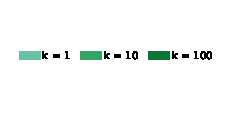
\includegraphics{./sources/plots/dyn-topk/legend-speedup.pdf}
\end{subfigure}\vspace{-20pt}
%
% Complex undirected
%
\begin{subfigure}[t]{.5\textwidth}
\begin{subfigure}[t]{.5\textwidth}
\centering
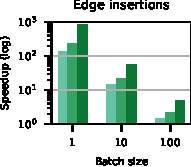
\includegraphics{./sources/plots/dyn-topk/speedup-undirected-small-diameter-addition.pdf}
\end{subfigure}\hfill
\begin{subfigure}[t]{.5\textwidth}
\centering
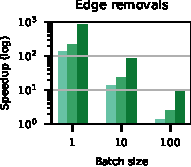
\includegraphics{./sources/plots/dyn-topk/speedup-undirected-small-diameter-removal.pdf}
\end{subfigure}\hfill
\caption{Complex undirected}
\label{fig:dyn-topk-speedup-cmplx-undir}
\end{subfigure}\hfill
%
% Complex directed
%
\begin{subfigure}[t]{.5\textwidth}
\begin{subfigure}[t]{.5\textwidth}
\centering
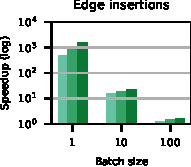
\includegraphics{./sources/plots/dyn-topk/speedup-directed-small-diameter-addition.pdf}
\end{subfigure}\hfill
\begin{subfigure}[t]{.5\textwidth}
\centering
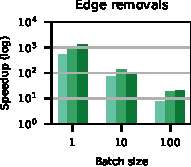
\includegraphics{./sources/plots/dyn-topk/speedup-directed-small-diameter-removal.pdf}
\end{subfigure}\hfill
\caption{Complex directed}
\label{fig:dyn-topk-speedup-cmplx-dir}
\end{subfigure}\medskip

% Road undirected
%
\begin{subfigure}[t]{.5\textwidth}
\begin{subfigure}[t]{.5\textwidth}
\centering
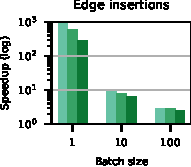
\includegraphics{./sources/plots/dyn-topk/speedup-undirected-high-diameter-addition.pdf}
\end{subfigure}\hfill
\begin{subfigure}[t]{.5\textwidth}
\centering
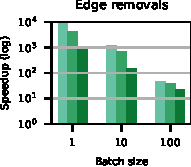
\includegraphics{./sources/plots/dyn-topk/speedup-undirected-high-diameter-removal.pdf}
\end{subfigure}\hfill
\caption{High-diameter undirected}
\label{fig:dyn-topk-speedup-road-undir}
\end{subfigure}\hfill
%
% Complex directed
%
\begin{subfigure}[t]{.5\textwidth}
\begin{subfigure}[t]{.5\textwidth}
\centering
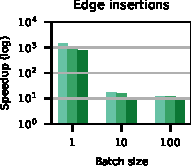
\includegraphics{./sources/plots/dyn-topk/speedup-directed-high-diameter-addition.pdf}
\end{subfigure}\hfill
\begin{subfigure}[t]{.5\textwidth}
\centering
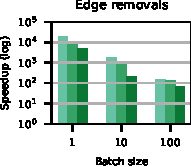
\includegraphics{./sources/plots/dyn-topk/speedup-directed-high-diameter-removal.pdf}
\end{subfigure}\hfill
\caption{High-diameter directed}
\label{fig:dyn-topk-speedup-road-dir}
\end{subfigure}
%
\caption{Geometric mean of the average speedups over all tested networks, for
different values of $k$ and batch sizes.
\Cref{fig:dyn-topk-speedup-cmplx-undir,fig:dyn-topk-speedup-cmplx-dir} show the
results for complex networks, whereas
\Cref{fig:dyn-topk-speedup-road-undir,fig:dyn-topk-speedup-road-dir} show
the results for road networks. Detailed numbers can be found in
\Cref{sec:dyn-topk-add-exp-complex,sec:dyn-topk-add-exp-road}.}
\label{fig:dyn-topk-speedups-summary}
\end{figure}

\begin{figure}[tb]
\centering
\begin{subfigure}[t]{\textwidth}
\centering
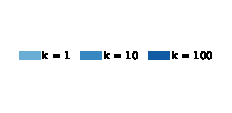
\includegraphics{./sources/plots/dyn-topk/legend-breakdown.pdf}
\end{subfigure}\vspace{-20pt}

% Complex undirected
\begin{subfigure}[t]{.5\textwidth}
\begin{subfigure}[t]{.5\textwidth}
\centering
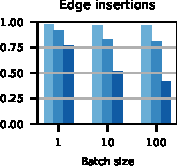
\includegraphics{./sources/plots/dyn-topk/breakdown-undirected-small-diameter-addition.pdf}
\end{subfigure}\hfill
\begin{subfigure}[t]{.5\textwidth}
\centering
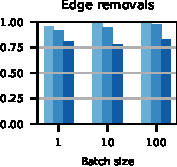
\includegraphics{./sources/plots/dyn-topk/breakdown-undirected-small-diameter-removal.pdf}
\end{subfigure}\hfill
\caption{Complex undirected}
\label{fig:dyn-topk-breakdown-cmplx-undir}
\end{subfigure}\hfill
%
% Complex directed
%
\begin{subfigure}[t]{.5\textwidth}
\begin{subfigure}[t]{.5\textwidth}
\centering
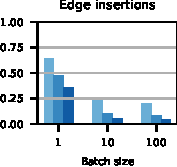
\includegraphics{./sources/plots/dyn-topk/breakdown-directed-small-diameter-addition.pdf}
\end{subfigure}\hfill
\begin{subfigure}[t]{.5\textwidth}
\centering
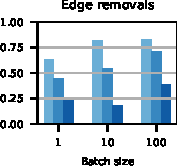
\includegraphics{./sources/plots/dyn-topk/breakdown-directed-small-diameter-removal.pdf}
\end{subfigure}\hfill
\caption{Complex directed}
\label{fig:dyn-topk-breakdown-cmplx-dir}
\end{subfigure}\medskip

% Road undirected
\begin{subfigure}[t]{.5\textwidth}
\begin{subfigure}[t]{.5\textwidth}
\centering
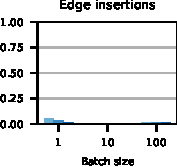
\includegraphics{./sources/plots/dyn-topk/breakdown-undirected-high-diameter-addition.pdf}
\end{subfigure}\hfill
\begin{subfigure}[t]{.5\textwidth}
\centering
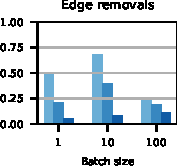
\includegraphics{./sources/plots/dyn-topk/breakdown-undirected-high-diameter-removal.pdf}
\end{subfigure}\hfill
\caption{High diameter undirected}
\label{fig:dyn-topk-breakdown-road-undir}
\end{subfigure}\hfill
%
% Road directed
%
\begin{subfigure}[t]{.5\textwidth}
\begin{subfigure}[t]{.5\textwidth}
\centering
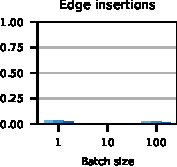
\includegraphics{./sources/plots/dyn-topk/breakdown-directed-high-diameter-addition.pdf}
\end{subfigure}\hfill
\begin{subfigure}[t]{.5\textwidth}
\centering
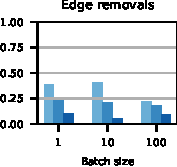
\includegraphics{./sources/plots/dyn-topk/breakdown-directed-high-diameter-removal.pdf}
\end{subfigure}\hfill
\caption{High diameter directed}
\label{fig:dyn-topk-breakdown-road-dir}
\end{subfigure}

\caption{Geometric mean of the average time spent by the dynamic algorithm
computing $\harmupp'(\cdot)$ \wrt the total time spent in updating the top-$k$ nodes
with highest closeness centrality over all the tested networks, for different
values of $k$ and batch sizes.
\Cref{fig:dyn-topk-breakdown-cmplx-undir,fig:dyn-topk-breakdown-cmplx-dir}
show the results for complex networks,
whereas
\Cref{fig:dyn-topk-breakdown-road-undir,fig:dyn-topk-breakdown-road-dir}
show the results for road networks.}
\label{fig:dyn-topk-breakdown}
\end{figure}

\Cref{fig:dyn-topk-speedup-cmplx-undir,fig:dyn-topk-speedup-cmplx-dir}
summarize the speedup of our dynamic algorithm on the static one for complex
networks while \Cref{fig:dyn-topk-breakdown-cmplx-undir,fig:dyn-topk-breakdown-cmplx-dir}
show the fraction of time spent by the dynamic algorithm computing $\harmupp'(\cdot)$ of
the affected vertices \wrt the algorithm's overall running time (\ie computing
$\harmupp'(\cdot)$ and the new top-$k$ ranking) for complex networks.
Detailed results for insertions in complex networks are reported in
\Cref{tab:dyn-topk-speed-ins-cmplx,tab:dyn-topk:time-ins-cmplx}.
%
For undirected networks, the geometric mean of the speedups over 100 single
edge insertions are always at least in the double-digit range for every instance.
Also, the speedups grow for bigger values of $k$, reaching an average speedup (over
all tested undirected instances) of \speedupComplexUndInsertKHundredBOne for
$k = 100$. A possible explanation for this pattern is that separating the top-$k$
vertices with highest closeness centrality from the others is harder for larger
values of $k$ and the dynamic algorithm does this faster because it exploits
precomputed values of $\harmupp'(\cdot)$. This is also clear from the left plot of
\Cref{fig:dyn-topk-breakdown-cmplx-undir}, as updating the ranking becomes more
expensive for larger values of $k$.

For larger batches of edge insertions, our dynamic algorithm yields diminishing
returns. This is expected because, the more the graph changes, the less accurate
the bounds $\harmupp'(\cdot)$ become. As we can clearly see from
\Cref{fig:dyn-topk-breakdown-cmplx-undir}, inaccurate bounds jeopardize the
performance of the dynamic algorithm since the recomputation of the ranking becomes
more expensive as we increase the batch size.
Nevertheless, averaging over all the undirected networks, with $k = 1$ the dynamic
algorithm handles batches of 100 edge insertions
\speedupComplexUndInsertKOneBHundred faster than the static algorithm,
\speedupComplexUndInsertKTenBHundred faster with $k = 10$, and
\speedupComplexUndInsertKHundredBHundred faster with $k = 100$.

Concerning directed graphs, the average speedups for single edge insertions are better
than for the undirected case: the average speedup over all the tested directed
networks are \speedupComplexDirInsertKOneBOne for $k = 1$,
\speedupComplexDirInsertKTenBOne for $k = 10$ and
\speedupComplexDirInsertKHundredBOne for $k = 100$.
%
This can be explained by the smaller number of affected vertices in directed networks
(see \Cref{tab:dyn-topk-affected-directed}). The performance of the dynamic
algorithm for directed networks seems to be more susceptible to the batch
size than for undirected networks; for example, for $k = 10$ and 10 edge insertions,
the average speedup is \speedupComplexDirInsertKTenBTen on
directed networks and \speedupComplexUndInsertKTenBTen on undirected networks,
while for 100 edge insertions the average speedup is
\speedupComplexDirInsertKTenBHundred and \speedupComplexUndInsertKTenBHundred
respectively.
%
Similarly to the undirected case, this is likely due to the inaccuracy of the
updated bounds as the dynamic algorithm spends the vast majority of its running
time in recomputing the ranking (see the left plot in
\Cref{fig:dyn-topk-breakdown-cmplx-dir}).

Speedups for edge removals on complex networks are summarized in the right of
\Cref{fig:dyn-topk-speedup-cmplx-undir,fig:dyn-topk-speedup-cmplx-dir} --
detailed results are reported in
\Cref{tab:dyn-topk-speed-rem-cmplx,tab:dyn-topk:time-rem-cmplx}.
Interestingly, for directed graphs, our algorithm handles removals faster than
insertions, whereas the performance does not change substantially \wrt insertions
in the undirected case. In general, for shortest-path based problems insertions
are easier to handle than removals; for example, pairwise distances can be
updated in $\Oh(n^2)$ time after an edge insertion, but not after an edge
removal~\cite{DBLP:journals/jacm/DemetrescuI04}. In our case, we know that
removals can only \emph{decrease} centrality. Thus, the upper bounds
of the centralities are still valid and, if none of the top-$k$ vertices
is affected, nothing needs to be done.
In insertions, on the contrary, any vertex could \emph{increase} its centrality
and become one of the top-$k$.
If the number of affected vertices is small -- as in most cases for directed graphs,
see \Cref{tab:dyn-topk-affected-directed} -- it is quite unlikely that a top-$k$
vertex is affected. This happens more often in undirected graphs, where often a larger
number of vertices are affected. Consequently, as shown in
\Cref{fig:dyn-topk-breakdown-cmplx-undir,fig:dyn-topk-breakdown-cmplx-dir},
updating the ranking is less expensive after an edge removal than after an edge
insertion.
%
As for insertions, speedups increase with $k$ and decrease with the batch
size: for single edge removals, the geometric mean of the speedups in
undirected graphs is \speedupComplexUndRemovalKOneBOne for $k=1$,
\speedupComplexUndRemovalKTenBOne for $k=10$, and
\speedupComplexUndRemovalKHundredBOne for $k=100$, whereas for directed graphs
it is \speedupComplexDirRemovalKOneBOne for $k=1$,
\speedupComplexDirRemovalKTenBOne for $k=10$, and
\speedupComplexDirRemovalKHundredBOne for $k=100$.
%
For edge removals, the decrease of the speedups \wrt the batch size is less severe
than for edge insertions; the bounds on the
closeness centrality after a batch of edge removals are likely to be tighter than the ones
computed after a batch of edge insertions, allowing \Cref{algo:nbcut-dyn-rem} to terminate
often earlier than \Cref{algo:nbcut-dyn-ins}.


\paragraph{Dynamic Road Networks}
%
\Cref{fig:dyn-topk-speedup-road-undir,fig:dyn-topk-speedup-road-dir} summarize
the speedups for directed and undirected road networks, respectively --
detailed results are shown in
\Cref{tab:dyn-topk-speed-ins-road,tab:dyn-topk-speed-rem-road,tab:dyn-topk:time-ins-road,tab:dyn-topk:time-rem-road} --
whereas
\Cref{fig:dyn-topk-breakdown-road-undir,fig:dyn-topk-breakdown-road-dir} show
the fraction of time spent by the dynamic algorithm updating $\harmupp'(\cdot)$ \wrt
the algorithm's overall running time.
%
As for complex networks, speedups in road networks are generally higher in
the directed case and they decrease with the batch size. However, differently
from complex networks, speedups generally decrease with $k$: If $k$ is large,
it is also more likely that some affected vertices are either among the top-$k$
or \enquote{overtake} one of the top-$k$, making the algorithm run \bfsbound more
often and thus slowing it down. The bar plots in the left of
\Cref{fig:dyn-topk-breakdown-road-undir,fig:dyn-topk-breakdown-road-dir}
also show that the running time of the dynamic algorithm is dominated by the
recomputation of the ranking, which is expected because closeness centrality
distinguishes vertices in complex networks less efficiently than in high-diameter
networks~\cite[Ch. 7]{newman2018networks}.
Nevertheless, even for $k = 100$, for a single edge insertion
the dynamic algorithm is on average \speedupStreetUndInsertKHundredBOne faster than
a static recomputation in undirected road networks
and \speedupStreetDirInsertKHundredBOne faster in directed road networks.
Furthermore, regarding multiple edge insertions, the dynamic
algorithm is faster than a static recomputation on all the considered instances and
for all the considered batch sizes.

Results for removals are significantly better: for $k = 1$ and single edge removals
the dynamic algorithm is on average
\speedupStreetUndRemovalKOneBOne faster in the undirected case and
\speedupStreetDirRemovalKOneBOne in the directed one, while
for $k = 100$ the speedups are \speedupStreetUndRemovalKHundredBOne
and \speedupStreetDirRemovalKHundredBOne, respectively.
%
As we described previously, the impact on the ranking due to edge
removals is in general lower than edge insertions, so the dynamic algorithm
spends less time on recomputing the ranking. This is also clear from the bar
plots in the right of
\Cref{fig:dyn-topk-breakdown-road-undir,fig:dyn-topk-breakdown-road-dir}:
after edge removals the fraction of time spent by the dynamic algorithm
updating $\harmupp'(\cdot)$ \wrt the total running time is greater than after edge
insertions.
%
Finally, concerning batches of 10 [100] edge removals, the dynamic algorithm is
on average two to three [one to two] orders of magnitude faster than a static
recomputation.

\section{Conclusions}
%
In this chapter, we addressed the problem of preserving an exact top-$k$
ranking of the vertices with highest closeness (including their exact score).
We implemented batch-dynamic algorithms for top-$k$
closeness centrality tailored to both complex and high-diameter networks.
Our dynamic algorithms are developed on top of the static algorithms for top-$k$
closeness centrality by Bergamini \etal~\cite{DBLP:journals/tkdd/BergaminiBCMM19};
in particular, they maintain upper bounds $\harmupp(\cdot)$ on the closeness
centrality of every vertex, which accelerates the computation of the top-$k$
vertices in practice.
By re-using such bounds as well as other precomputed information, we are able
to significantly reduce the number of operations required to update the most
central vertices in the graph after multiple graph updates.

As a result, for single edge updates, we achieve high speedups \change{on a}
static recomputation, in line with results obtained by other dynamic algorithms
for related
problems~\cite{DBLP:journals/im/BergaminiM16,DBLP:conf/wea/BergaminiMOS17,
DBLP:conf/socialcom/GreenMB12,DBLP:conf/asunam/KasCC13} -- confirming that
efforts in developing dynamic algorithms are well spent.
%
As we increase the batch sizes, our strategy yield\change{s} diminishing
returns. This is expected because, the more the graph changes, the less precise
the upper bounds $\harmupp'(\cdot)$ become and this impacts the performance of
our dynamic algorithms. Nevertheless, experimental data show that, averaging
results over the tested instances, our dynamic algorithms are always faster
than a static recomputation. \change{In contrast to} most existing algorithms
for updating shortest-path based centralities \change{that require $\Oh(n^2)$
additional memory,} the techniques we propose require an
amount of memory that is \change{only} linear in $n$. Although storing more data
(\eg the distances computed during \bfscut on the initial graph) might lead to
even higher speedups, a quadratic memory footprint would not allow us to target
networks with millions of vertices. An interesting question is whether the
memory requirements of other dynamic algorithms for related problems can be
reduced by using techniques similar to the ones we presented in this chapter.

A possible direction for future research is the extension of our strategies
for batch updates to other centrality
measures such as betweenness -- for which a static algorithm for finding the
top-$k$ vertices with highest betweenness has already been proposed in
Ref.~\cite{DBLP:conf/www/LeeC14}. Thus, an interesting question is whether this
algorithm can be further improved and/or efficiently updated in fully-dynamic
networks.

%%%%%%%%%%%%%%%%%%%%%%%%%%%%%%%%%%%%%%%%%%%%%%%%%%%%%%%%%%%%%%%%%%%%%%%%
\chapter{Parallel Approximation of Betweenness Centrality}
\label{ch:betweenness-approx}
% Labels: approximate, static, distance-based, parallel
%%%%%%%%%%%%%%%%%%%%%%%%%%%%%%%%%%%%%%%%%%%%%%%%%%%%%%%%%%%%%%%%%%%%%%%%

\section{Introduction}
%
With large datasets being the rule and not the exception today, approximation
is frequently applied~\cite{DBLP:books/tf/18/2018aam-1} to problems that cannot be
solved exactly within a desired time budget, including polynomial-time
problems~\cite{DBLP:conf/esa/BorassiN16}. We focus on a particular subclass of
approximation algorithms: \emph{sampling algorithms}. They sample data
according to some (usually algorithm-specific) probability distribution,
perform some computation on the sample and induce a result for the full
dataset.

More specifically, we consider \emph{adaptive} sampling (ADS) algorithms --
also called \emph{progressive} sampling algorithms. Here, the number of samples
that are required is not statically computed (\eg from the input instance) but
also depends on the data that has been sampled so far. While non-adaptive
sampling algorithms can often be parallelized trivially by drawing multiple
samples in parallel, adaptive sampling constitutes a challenge for
parallelization: checking the stopping condition of an ADS algorithm requires
access to all the samples drawn so far and thus mandates some form of
synchronization.


\paragraph{Motivation and Contribution}
%
Our initial motivation was a parallel implementation of the sequential
state-of-the-art approximation algorithm \kadabra~\cite{DBLP:conf/esa/BorassiN16} for
betweenness centrality (\betw) approximation. Betweenness is a very popular
centrality measure in network analysis, see
\Cref{sec:prelim:path-based-centrality,sec:betw-apx:betw-apx} for more details.
To the best of our knowledge, parallel adaptive sampling has not received a
generic treatment yet. Hence, we propose techniques to parallelize ADS
algorithms in a generic way, while scaling to large numbers of threads.
%
While we turn to \kadabra to demonstrate the effectiveness of the proposed
algorithms, our techniques can be adjusted easily to other ADS algorithms.

%
We introduce two new parallel ADS algorithms, which we call \localframe
and \sharedframe.
Both algorithms try to avoid extensive synchronization when checking the
stopping condition. This is done by maintaining multiple copies of the sampling state
and ensuring that the stopping condition is never checked on a copy
of the state that is currently being written to.
%
\Localframe is designed to use the least amount of synchronization possible
-- at the cost of an additional memory footprint of
$\Theta(n_s)$ per thread, where $n_s$ denotes the size of the sampling
state.
%
This algorithm performs only atomic \texttt{load-acquire} and
\texttt{store-release} operations for synchronization, but no
expensive read-modify-write operations (like \texttt{CAS} or \texttt{fetch-add}).
%
\Sharedframe, in turn, aims instead at meeting a
desired trade-off between memory footprint and synchronization overhead.
In contrast to \localframe, it requires only $\Theta(1)$
additional memory per thread, but
uses atomic read-modify-write operations (\eg \texttt{fetch-add}) to accumulate samples.
%
We also propose the deterministic \indexedframe algorithm; it
guarantees that the results of two different executions is the same
for a fixed random seed, regardless of the number of threads.

Our experimental results show that \localframe, \sharedframe, and \indexedframe
achieve parallel speedups of $\onedigit{\adsParallelSuLf}\times$,
$\onedigit{\adsParallelSuSf}\times$,
and $\onedigit{\adsParallelSuDt}\times$ on 32 cores, respectively.
Using the same number of cores, our OpenMP-based parallelization (functioning as a baseline)
only yields a speedup of $\onedigit{\adsParallelSuNaive}\times$;
thus, our algorithms are up to $\onedigit{\adsSuSfVsOmp}\times$ faster.
Moreover, also due to implementation improvements and parameter tuning,
our best algorithm performs adaptive sampling $\onedigit{\adsSuSfVsOriginal}\times$
faster than the existing implementation of \kadabra (when all implementations use 32 cores).
\bibnotes{
The contributions presented in this chapter were published in the Proceedings
of the \emph{Twenty-Fifth European Conference on Parallel Processing (Euro-Par
2019)}. My contributions involve the development of the \indexedframe algorithm
with bounded memory complexity (\Cref{sec:betw-apx:bounded-mem-indexed-frame})
in collaboration with Alexander van der Grinten and
the implementation of all presented algorithms. The rest is
joint work with Alexander van der Grinten and Henning Meyerhenke. Proofs to
which I did not contribute are omitted and can be found in the original
paper~\cite{DBLP:conf/europar/GrintenAM19}.}

\section{Preliminaries and Baseline for Parallelization}
%
\subsection{Basic Definitions}
\label{sec:betw-apx:basic-defs}
%
\paragraph{Memory Model}
%
Throughout this chapter, we target a multi-threaded shared-memory machine
with $T$ threads. We work in the C11 memory model~\cite{ISO2012III}.
The weakest operations in this model are \texttt{load-relaxed} and \texttt{store-relaxed}
operations; those only guarantee the atomicity of the memory access
(\ie they guarantee that no \emph{tearing} occurs)
but no ordering at all. Hence, the order in which \texttt{store-relaxed}
writes become visible to \texttt{load-relaxed} reads can differ from the
order in which the stores and loads are performed by individual threads.
Additionally, \texttt{load-acquire} and \texttt{store-release}
do provide ordering guarantees:
if thread $t_0$ writes a word $X$ to a given memory location using \texttt{store-release}
\emph{and} thread $t_1$ reads $X$ using \texttt{load-acquire} from the same memory location,
then all store operations -- whether atomic or not --
done by thread $t_0$ \emph{before} the store of $X$
become visible to all load operations done by thread $t_1$ \emph{after} the load of $X$.
We note that C11 defines even stronger ordering guarantees that we do not require in
this chapter.
Furthermore, on a hardware level, x86\_64 implements a stronger \emph{total store order};
thus, \texttt{load-acquire} and \texttt{store-release} compile to plain
load and store instructions and our \localframe algorithm does not perform \emph{any}
synchronization instructions on x86\_64.

\paragraph{Adaptive sampling}
%
\begin{algorithm}[bt]
\caption{Generic Adaptive Sampling}
\label{algo:generic-adaptive-sampling}
\begin{algorithmic}[1]
    \TopComment{Variable initialization}
	\State $d \gets$ new sampling state structure
	\State $d\mathtt{.data} \gets (0, \ldots, 0)$ \Comment{Sampled data}
	\State $d\mathtt{.num} \gets 0$ \Comment{Number of samples}
    \TopComment{Main loop}
    \While{\textbf{not} \Call{checkForStop}{$d$}}
		\State $d\mathtt{.data} \gets d\mathtt{.data} \circ \Call{sample}{\null}$
		\State $d\mathtt{.num} \gets d\mathtt{.num} + 1$
	\EndWhile
\end{algorithmic}
\end{algorithm}
%
For our techniques to be applicable, we expect that an ADS
algorithm behaves as depicted in \Cref{algo:generic-adaptive-sampling}: it
iteratively samples data (in \Call{sample}{}) and aggregates it
(using some operator $\circ$) until a stopping condition (\Call{checkForStop}{})
determines that the data sampled so far is sufficient to
return an approximate solution within the required accuracy.
This condition does not only consider the number of samples
($d\mathtt{.num}$),
but also the sampled data
($d\mathtt{.data}$). Throughout this chapter, we denote the size
of that data (\ie the number of elements of $d.\mathtt{data}$) by $n_s$.
We assume that the stopping condition needs to be checked on
a \emph{consistent} state, \ie a state of $d$ that can
occur in a sequential
execution.\footnote{That is, $d\mathtt{.num}$ and all entries of $d\mathtt{.data}$ must
result from an integral sequence of samples -- parallelization
would be trivial otherwise.}
Furthermore, to make parallelization feasible at all, we need to assume
that $\circ$ is associative.
For concrete examples of stopping conditions, we refer
to~\Cref{sec:betw-apx:kad-algo,sec:betw-apx:stopping-condition}.

\subsection{Betweenness Centrality and its Approximation}
\label{sec:betw-apx:betw-apx}
%
\emph{Betweenness Centrality} ($\betw$) is one of the most popular vertex
centrality measures for network analysis (see
\Cref{sec:prelim:path-based-centrality}).
Th betweenness of a vertex $u \in V$ is defined as:
%
\[
\betw(u) := \sum_{\substack{x,y \in V \setminus \set{u}\\x\neq y,\ \sigma_{x,y} \neq 0}}
\frac{\sigma_{x,y}(u)}{\sigma_{x,y}},
\]
%
where $\sigma_{x, y}$ is the number of shortest $x$-$y$ paths and $\sigma_{x, y}(u)$
is the number of shortest $x$-$y$ paths that contain $u$.
Betweenness is extensively used to identify the key vertices in large networks,
\eg cities in a transportation network~\cite{guimera2005worldwide} or lethality
in protein networks~\cite{jeong2001lethality}.

Unfortunately, $\betw(\cdot)$ is rather expensive to compute: the standard exact
algorithm by Brandes~\cite{brandes2001faster} has time complexity $\Theta(n\cdot m)$
for unweighted graphs. Moreover, unless the Strong Exponential Time Hypothesis (SETH)
fails, this asymptotic running time cannot be improved~\cite{DBLP:journals/entcs/BorassiCH16}.
Numerous approximation algorithms for betweenness centrality have been developed --
we refer to \Cref{sec:betw-apx:related-work} for an overview.
The state of the art of these approximation algorithms is the \kadabra
algorithm~\cite{DBLP:conf/esa/BorassiN16} of Borassi and Natale, which happens to
be an ADS algorithm.
%
With probability $(1 - \delta)$, \kadabra approximates the $\betw(\cdot)$ values
of the vertices within an additive error of $\pm\epsilon$ in nearly-linear
time complexity, where $\delta$ and $\epsilon$ are user-specified constants.

While our techniques apply to any ADS algorithm, we recall that, as a case
study, we focus on scaling the \kadabra algorithm to large number of threads.

\subsection{The \kadabra Algorithm}
\label{sec:betw-apx:kad-algo}
%
At each iteration, \kadabra samples a vertex pair $(s, t)$ of $G = (V, E,
w)$ uniformly at random and then selects a shortest $s$-$t$-path
uniformly at random (\Call{sample}{} in \Cref{algo:generic-adaptive-sampling}).
After $\tau$ iterations, this results in a sequence of randomly selected
shortest paths $(\pi_1, \pi_2, \ldots, \pi_\tau)$. From those paths,
$\betw(u)$ is estimated as:
%
\[
    \bapx(u) = \frac 1\tau\sum_{i = 1}^\tau x_i(u),\quad x_i(u) =
    \begin{cases}
        1 & \text{ if } v \in \pi_i\\
        0 & \text{ otherwise}.
    \end{cases}
\]

$\sum_{i = 1}^\tau x_i$ is exactly the sampled data ($d\mathtt{.data}$)
that the algorithm has to store -- the accumulation $\circ$ in
\Cref{algo:generic-adaptive-sampling} sums $x_i$ over $i$.
To compute the stopping condition (\Call{checkForStop}{} in
\Cref{algo:generic-adaptive-sampling}), \kadabra maintains the
invariants:

\begin{equation}
\label{eq:betw-apx:kadabra-invariants}
\Pr(\betw(u) \le \bapx(u) - f) \le \delta_L(u)\quad \text{ and }\quad
\Pr(\betw(u) \ge \bapx(u) + g) \le \delta_U(u)
\end{equation}
%
for two functions $f = f(\bapx(u), \delta_L(u), \tau_{\max}, \tau)$
and $g = g(\bapx(u), \delta_U(u), \tau_{\max}, \tau)$ depending on
a maximum number $\tau_{\max}$ of samples and per-vertex probability
constants $\delta_L$ and $\delta_U$ (more details in the original
paper~\cite{DBLP:conf/esa/BorassiN16}).
%
The value of those constants are computed in a preprocessing phase -- mostly
consisting of computing an upper bound of the diameter of the graph. $\delta_L$
and $\delta_U$ satisfy $\sum_{u \in V} \delta_L(u) + \delta_U(u) \le \delta$
for a user-specified parameter $\delta \in (0, 1)$. Thus, the algorithm
terminates once $f, g < \epsilon$; with probability $(1 - \delta)$, the result
is correct with an absolute error of $\pm\epsilon$.
%
We note that checking the stopping condition of \kadabra on an
inconsistent state leads to incorrect results. For example, this can
be seen from that fact that $g$ is increasing with $\bapx(\cdot)$ and
decreasing with $\tau$, see \Cref{sec:betw-apx:stopping-condition}.


\subsection{The Stopping Condition in Detail}
\label{sec:betw-apx:stopping-condition}
%
In this section, we illustrate the stopping condition more in detail and
show that evaluating it in a consistent state is crucial for the correctness
of the algorithm.
The functions $f$ and $g$ we mentioned in \Cref{eq:betw-apx:kadabra-invariants}
are defined as~\cite{DBLP:conf/esa/BorassiN16}:
%
\begin{align*}
    f(\bapx(u), \delta_{L}(u), \tau_{\max}, \tau) &=
  \frac{1}{\tau}\left(\log\frac{1}{\delta_{L}(u)}\right)
   \left(
  \frac{1}{3} - \frac{\tau_{\max}}{\tau}
  + \sqrt{\left(\frac{1}{3} - \frac{\tau_{\max}}{\tau} \right)^2 +
  \frac{2\bapx(u)\tau_{\max}}{\log\frac{1}{\delta_{L}(u)}}}
  \right)\\
  g(\bapx(u), \delta_{U}(u), \tau_{\max}, \tau) &=
  \frac{1}{\tau}\left(\log\frac{1}{\delta_{U}(u)}\right)
  \left(
  \frac{1}{3} + \frac{\tau_{\max}}{\tau}
  + \sqrt{\left(\frac{1}{3} + \frac{\tau_{\max}}{\tau} \right)^2 +
  \frac{2\bapx(u)\tau_{\max}}{\log\frac{1}{\delta_{U}(u)}}}
  \right),
\end{align*}
%
where $\bapx(u)$ is the approximation of the betweenness centrality
of vertex $u$ obtained after $\tau$ samples.
When the stopping condition is evaluated, $f$ and $g$ are computed for every
vertex of the graph and the algorithm terminates if:
%
\[
f(\bapx(u), \delta_{L}(u), \tau_{\max}, \tau) \le \epsilon
\quad \text{and} \quad
g(\bapx(u), \delta_{U}(u), \tau_{\max}, \tau) \le \epsilon
\]
%
hold for every vertex $u \in V$.
It is straightforward to verify that both $f$ and $g$ grow with
$\bapx(u)$ but that $g$ decreases with $\tau$. Thus, evaluating
the stopping condition with inconsistent data (\eg if accesses to
$\tau$ and $\bapx(u)$ are not synchronized) could lead to an
erroneous termination of the algorithm.

\subsection{First Attempts at \kadabra Parallelization}
\label{sec:betw-apx:first-attempts}
%
In the original \kadabra implementation,\footnote{Available
at \url{https://github.com/natema/kadabra}} a lock is used
to synchronize concurrent access to the sampling state.
As a first attempt to improve the scalability, we consider an
algorithm that iteratively computes a fixed number of
samples in parallel (\eg using an OpenMP \texttt{parallel for}
loop) and checks the stopping condition afterwards.
%
While sampling, atomic increments are used to update the global
sampling data. This algorithm is arguably the \enquote{natural}
OpenMP-based parallelization of an ADS algorithm and can be
implemented in a few extra lines of code.
%
Moreover, it already improves upon the original parallelization.
As shown by the experiments in \Cref{sec:betw-apx:experiments}
however, further significant improvements in performance
are possible by switching to more lightweight synchronization.

\section{Scalable Parallelization Techniques}
%
To improve upon the OpenMP parallelization from
\Cref{sec:betw-apx:first-attempts}, we have to avoid to synchronization barrier
before the stopping condition can be checked.
%
This is the objective of our \emph{epoch-based} algorithms that constitute the
main contribution of this chapter. In \Cref{sec:betw-apx:epoch-framework}, we
formulate the main idea of our algorithms as a general framework. The
subsequent subsections present specific algorithms based on this framework and
discuss the trade-offs between them.

\subsection{Epoch-based Framework}
\label{sec:betw-apx:epoch-framework}

\begin{figure}[t]%
\begin{subfigure}[t]{.48\textwidth}
\centering
\fbox{\begin{tabular}{r@{\quad}l@{\quad}l}
	\textsf{int} & \texttt{epoch} &$\gets e$ \\
	\textsf{int} & \texttt{num} &$\gets 0$\\
	\textsf{int} & \texttt{data}[$n_s$] &$\gets (0, \ldots, 0)$
\end{tabular}}%
\caption{Structure of a state frame (SF) for epoch $e$.
\texttt{num}: Number of samples, \texttt{data}: Sampled data}%
\label{fig:betw-apx:sf}
\end{subfigure}\hfill
\begin{subfigure}[t]{.48\textwidth}
\centering
\begin{tabular}{r@{\quad}l@{\quad}l}
	\textsf{bool} & \texttt{stop} &$\gets$ \false\\
	\textsf{int} & \texttt{epochToRead} &$\gets 0$\\
	SF $\ast$ & \texttt{sfFin[$T$]} &$\gets (\nil, \ldots, \nil)$
\end{tabular}%
\caption{Shared variables}%
\label{fig:betw:apx:globalvars}
\end{subfigure}%
\caption{Data structures used in epoch-based algorithms, including initial values}%
\label{fig:betw-apx:epoch-state}
\end{figure}

In our epoch-based algorithms, the execution of each thread is subdivided into
a sequence of discrete \emph{epochs}.
During an epoch, each thread iteratively collects samples; the stopping
condition is only checked at the end of an epoch.
The crucial advantage of this approach is that the end of an epoch
\emph{does not} require global synchronization. Instead, our
framework guarantees the consistency of the sampled data by
maintaining multiple copies of the sampling state.

As an invariant, it is guaranteed that no thread writes to a copy of the state
that is currently being read by another thread. This is achieved as follows:
each copy of the sampling state is labeled by an \emph{epoch number} $e$, \ie a
monotonically increasing integer that identifies the epoch in which the data
was generated. When the stopping condition has to be checked, all threads
advance to a new epoch $e + 1$ and start writing to a new copy of the sampling
state.
The stopping condition is only verified after all threads have finished this
transition and it only takes the sampling state of epoch $e$ into account.

More precisely, the main data structure that we use to store the sampling
state is called a \emph{state frame} (SF). Each SF $f$ (depicted
in \Cref{fig:betw-apx:sf}) consists of (i) an epoch number
($f.\mathtt{epoch}$), (ii) a number of samples ($f.\mathtt{num}$), and (iii)
the sampled data ($f.\mathtt{data}$).
The latter two symbols directly correspond to $d.\mathtt{num}$ and
$d.\mathtt{data}$ in our generic formulation of an ADS algorithm
(\Cref{algo:generic-adaptive-sampling}).
%
Aside from the SF structures, our framework maintains three
global variables that are shared among all threads
(depicted in \Cref{fig:betw:apx:globalvars}): (i)
a simple Boolean flag \texttt{stop} to determine if
the algorithm should terminate, (ii) a variable
\texttt{epochToRead} that stores the number of the epoch
we want to check the stopping condition on, and (iii)
a pointer $\mathtt{sfFin}[t]$ for each thread $t$
that points to a SF finished by thread $t$.
%
Incrementing \texttt{epochToRead} is our synchronization
mechanism to notify all threads that they should advance to a new epoch.
\Cref{fig:betw-apx:epoch-advance} visualizes such an epoch transition.
In particular, it depicts the update of the \texttt{sfFin} pointers
after an epoch transition is initiated by incrementing
\texttt{epochToRead}.

\begin{figure}[t]
\centering
\begin{tikzpicture}[sfstyle/.style={
	draw,rectangle,minimum width=1.1cm,minimum height=1.1cm,align=center,font=\scriptsize
}]
	\node[draw,rectangle] at (5,2) {$\mathtt{epochToRead} = 5$};

	\draw (-4,0) -- (6,0);
	\node[above right=0.15cm and 0cm] at (-4,0) {Thread 2};
	\node[below right=0.15cm and 0cm] at (-4,0) {Thread 9};

	\node[sfstyle,dashed] at (0,0.8) (sf00) {SF of\\epoch\\4};
	\node[sfstyle,right=0.5cm of sf00] (sf01) {SF of\\epoch\\5};
	\node[sfstyle,right=0.5cm of sf01] (sf02) {SF of\\epoch\\6};
	\node[sfstyle,right=0.5cm of sf02] (sf03) {$\ldots$};
	\node[text width=1.8cm,align=right,above left=-0.5cm and 1.5cm of sf00] (efin0) {$\mathtt{sfFin}[2]$};
	\node[text width=1.8cm,align=right,above=0cm of efin0] (csf0) {$f_\mathrm{sam}$};
	\draw[->,cyan,thick] (efin0.east) to[out=30,in=130] (sf01.north);
	\draw[->,orange,thick] (csf0.east) to[out=20,in=130] (sf02.north);

	\node[sfstyle] at (0,-0.8) (sf10) {SF of\\epoch\\4};
	\node[sfstyle,right=0.5cm of sf10] (sf11) {SF of\\epoch\\5};
	\node[sfstyle,right=0.5cm of sf11] (sf12) {SF of\\epoch\\6};
	\node[sfstyle,right=0.5cm of sf12] (sf13) {$\ldots$};
	\node[text width=1.8cm,align=right,below left=-0.5cm and 1.5cm of sf10] (efin1) {$\mathtt{sfFin}[9]$};
	\node[text width=1.8cm,align=right,below=0cm of efin1] (csf1) {$f_\mathrm{sam}$};
	\draw[->,cyan,thick] (efin1.east) to[out=-30,in=-130] (sf10.south);
	\draw[->,orange,thick] (csf1.east) to[out=-20,in=-130] ([xshift=-0.2cm]sf11.south);
	\draw[->,cyan,dashed,thick] (efin1.east) to[out=-30,in=-130] ([xshift=0.2cm]sf11.south);
	\draw[->,orange,dashed,thick] (csf1.east) to[out=-20,in=-130] (sf12.south);
\end{tikzpicture}


\caption{Transition after $\mathtt{epochToRead}$ is set to $5$. Thread 2 already
writes to the SF of epoch~6 (using the $f_\mathrm{sam}$ pointer).
Thread 9 still writes to the SF of epoch~5 but
advances to epoch~6 once it checks $\mathtt{epochToRead}$ (dashed orange line).
Afterwards, thread 9 publishes its SF of epoch~5 to $\mathtt{sfFin}$ (dashed blue line).
Finally, the stopping condition is checked using both SFs of epoch~5
(\ie the SFs now pointed to by $\mathtt{sfFin}$).}
\label{fig:betw-apx:epoch-advance}
\end{figure}

\begin{algorithm}[t]
\footnotesize
\caption{\footnotesize Epoch-based Approach}
\label{algo:epoch-based-approach}

\begin{minipage}[t]{.48\textwidth}
Per-thread variable initialization:
\begin{algorithmic}
    \State $e_\mathrm{sam} \gets 1$
    \State $f_\mathrm{sam} \gets$ new SF for $e_\mathrm{sam} = 1$
    \If{$t = 0$}
        \State $e_\mathrm{chk} \gets 0$
        \State $\mathit{inCheck} \gets \false$
    \EndIf
\end{algorithmic}

Main loop for thread $t$:
\begin{algorithmic}[1]
    \Loop
        \State $\mathit{doStop} \rlxmove \mathtt{stop}$ \label{line:epoch-based:main-loop}
        \If{$\mathit{doStop}$}
            \State \textbf{break}
        \EndIf
        \State $f_\mathrm{sam}\mathtt{.data}
            \gets f_\mathrm{sam}\mathtt{.data} \circ \Call{sample}{\null}$
        \State $f_\mathrm{sam}\mathtt{.num}
            \gets f_\mathrm{sam}\mathtt{.num} + 1$
        \State $r \rlxmove \mathtt{epochToRead}$ \label{line:epoch-based:advance-epoch}
        \If{$r =\ e_\mathrm{sam}$}
            \State reclaim SF of epoch $e_\mathrm{sam} - 1$ \label{line:epoch:based:reclaim}
            \State \texttt{sfFin}[t] $\storerel$ $f_\mathrm{sam}$ \label{line:epoch-based:publish}
            \State $e_\mathrm{sam} \gets e_\mathrm{sam} + 1$
            \State $f_\mathrm{sam} \gets$ new SF for $e_\mathrm{sam}$ \label{line:epoch-based:new-sf}
        \EndIf
        \If{$t = 0$} \label{line:epoch-based:thread-zero-call}
            \State \Call{checkFrames}{\null}
        \EndIf
    \EndLoop
\algstore{epochbased}
\end{algorithmic}
\end{minipage}\hfill
\begin{minipage}[t]{.48\textwidth}
Check of stopping condition by thread $0$:
\begin{algorithmic}[1]
\algrestore{epochbased}
    \Procedure{checkFrames}{\null}
        \If{\textbf{not} $\mathit{inCheck}$} \label{line:epoch-based:check-cycle}
            \State $e_\mathrm{chk} \gets e_\mathrm{chk} + 1$
            \State $\mathtt{epochToRead} \rlxmove e_\mathrm{chk}$
            \State $\mathit{inCheck} \gets \true$
        \EndIf
        \For{$t = 0$ \textbf{to} $T - 1$} \label{line:epoch-based:check-frames}
            \State $f_\mathrm{fin} \loadacq \mathtt{sfFin}[t]$ \label{line:epoch-based:subscribe}
            \If{$f_\mathrm{fin} = \nil$}
                \State \Return
            \EndIf
            \If{$f_\mathrm{fin}.\mathtt{epoch} \neq e_\mathrm{chk}$}
                \State \Return
            \EndIf
        \EndFor
        \State $d \gets$ new SF for accumulation
        \For{$t = 0$ \textbf{to} $T$} \label{line:epoch-based:accumulate}
            \State $f_\mathrm{fin} \rlxmove \mathtt{sfFin}[t]$
            \State $d\mathtt{.data}
                \gets d\mathtt{.data} \circ f_\mathrm{fin}\mathtt{.data}$
            \State $d\mathtt{.num}
                \gets d\mathtt{.num} + f_\mathrm{fin}\mathtt{.num}$
        \EndFor
        \If{\Call{checkForStop}{$d$}} \label{line:epoch-based:convergence}
            \State $\mathtt{stop} \rlxmove \true$ \label{line:epoch-based:do-stop}
        \EndIf
        \State $\mathit{inCheck} \gets \false$
    \EndProcedure
\end{algorithmic}
\end{minipage}
\end{algorithm}


\Cref{algo:epoch-based-approach} states the pseudocode of our framework.
By $\rlxmove$, $\loadacq$, and $\storerel$, we denote relaxed memory access,
\texttt{load-acquire} and \texttt{store-release}, respectively (see
\Cref{sec:betw-apx:basic-defs}).
In the algorithm, each thread maintains an epoch number $e_\mathrm{sam}$.
To be able to check the stopping condition,
thread 0 maintains another epoch number $e_\mathrm{chk}$.
Indeed, thread 0 is the only thread that evaluates the stopping condition
(in \Call{checkFrames}{}) after accumulating the SFs from all threads.
The \Call{checkFrames}{} procedure determines whether there is an ongoing check
for the stopping condition ($\mathit{inCheck}$ is \true;
\Cref{line:epoch-based:check-cycle}).
If that is not the case, a check is initiated (by incrementing
$e_\mathrm{chk}$ and all threads are signaled to advance to the
next epoch (by updating \texttt{epochToRead}).
Note that $\mathit{inCheck}$ is needed to prevent thread 0
from repeatedly incrementing $e_\mathrm{chk}$ without processing
data from the other threads. Afterwards, \Call{checkFrames}{}
only continues if all threads $t$ have published their SFs for
checking (\ie $\mathtt{sfFin}[t]$ points to a SF of epoch
$e_\mathrm{chk}$; \Cref{line:epoch-based:check-frames}).
%
Once that happens, those SFs are accumulated
(\Cref{line:epoch-based:accumulate}) and the stopping condition is
checked on the accumulated data (\Cref{line:epoch-based:convergence}).
Eventually, the termination flag (\texttt{stop}, \Cref{line:epoch-based:do-stop})
signals to all threads that they should stop sampling.
%
The main algorithm, on the other hand, performs a loop until this
flag is set (\Cref{line:epoch-based:main-loop}).
Each iteration collects one sample and writes the results to the
current SF ($f_\mathrm{sam}$).
If a thread needs to advance to a new epoch (because
an incremented \texttt{epochToRead} is read in \Cref{line:epoch-based:advance-epoch}),
it publishes its current SF to \texttt{sfFin} and starts writing
to a new SF ($f_\mathrm{sam}$; \Cref{line:epoch-based:new-sf}).
Note that the memory used by old SFs can be reclaimed (\Cref{line:epoch:based:reclaim});
note, however, that there is no SF for epoch 0).
How exactly this is done is left to the algorithms described in later
subsections.

\begin{proposition}[\cite{DBLP:conf/europar/GrintenAM19}]
\Cref{algo:epoch-based-approach} always checks the stopping
condition on a consistent state; in particular, the epoch-based
approach is correct.
\end{proposition}


\subsection{\Localframe and \sharedframe Algorithm}
We present two epoch-based algorithms relying on the general framework from the
previous section: namely, the \localframe and the \sharedframe
algorithm.
Furthermore, in
\Cref{sec:betw-apx:indexed-frame,sec:betw-apx:bounded-mem-indexed-frame},
we present two variants of the deterministic \indexedframe algorithm -- as both
\localframe and \sharedframe are non-deterministic.
\Localframe and \sharedframe are both based on the pseudocode of
\Cref{algo:epoch-based-approach}. They differ, however, in their allocation
and reuse of SFs (\Cref{line:epoch:based:reclaim} of the pseudocode).
The \localframe algorithm allocates one pair of SFs per thread and cycles
through both SFs of that pair (\ie epochs with even numbers are assigned
to the first SF while odd epochs use the second SF).
%
This yields a per-thread memory requirement of $\Oh(n_s)$; as before, $n_s$ denotes
the size of the sampling state. The \sharedframe algorithm reduces this memory
requirement to $\Oh(1)$ by only allocating $F$ pairs of SFs in total, for a
constant number $F$. Thus, $T/F$ threads share a SF in each epoch and atomic
\texttt{fetch-add} operations need to be used to write to the SF. The parameter
$F$ can be used to balance the memory bandwidth and synchronization costs -- a
smaller value of $F$ lowers the memory bandwidth required during aggregation
but leads to more cache contention due to atomic operations.

\subsection{Synchronization Costs}
\label{sec:betw-apx:sync-costs}
%
In \Cref{algo:epoch-based-approach}, all synchronization of threads
$t > 0$ is done wait-free in the sense that the threads only have to
stop sampling for $\Theta(1)$ instructions to communicate with other threads
(\ie to check \texttt{epochToRead}, update per-thread state and
write to $\mathtt{sfFin}[t]$).
At the same time, thread $t = 0$ generally needs to check all \texttt{sfFin}
pointers. Taken together, this yields the following statement:

\begin{proposition}[\cite{DBLP:conf/europar/GrintenAM19}]
In each iteration of the main loop, threads $t > 0$ of \localframe and
\sharedframe algorithms spend $\Theta(1)$ time to wait for other threads.
Thread $t = 0$ spends up to $\Oh(T)$ time to wait for other threads.
\end{proposition}

In particular, the synchronization cost does not depend on the
problem instance -- this is in contrast to the OpenMP
parallelization (\Cref{sec:betw-apx:first-attempts}) in which
threads can idle for $\Oh(\mathcal{S})$ time, where
$\mathcal{S}$ denotes the time complexity of a sampling
operation (\eg $\mathcal{S} = \Oh(n + m)$ in the case of
\kadabra).

Nevertheless, this advantage in synchronization costs
comes at a price: the accumulation of the sampling
data requires additional evaluations of $\circ$.
The \localframe algorithm requires $\Oh(Ts)$ evaluations,
whereas the \sharedframe requires $\Oh(Fs)$.
%
No accumulation is necessary in the OpenMP baseline.
As can be seen in \Cref{algo:epoch-based-approach},
we perform the accumulation in a single thread (\ie
thread 0).
Compared to a parallel implementation (\eg using
parallel reductions), this strategy requires no additional
synchronization and has a favorable memory access pattern
(as the SFs are read linearly). A disadvantage, however,
is that there is a higher latency (depending on $T$) until
the algorithm detects that it is able to stop.
In \Cref{sec:betw-apx:termination-latency},
we discuss how a constant latency can be achieved
heuristically.

\section{Optimization and Tuning}
%
\subsection{Improvements to the \kadabra Implementation}
\label{sec:betw-apx:kad-improvements}
%
In the following, we document some improvements to the sequential \kadabra
implementation of Borassi and Natale~\cite{DBLP:conf/esa/BorassiN16}.
First, for undirected graphs, we avoid searching for non-existing
shortest paths between a pair $(s, t)$ of randomly selected
vertices by checking if $s$ and $t$ belong to the same connected
component.\footnote{Connected components are computed along with
the diameter during preprocessing.}
%
Then, we reduce the memory footprint of the sampling procedure:
the original \kadabra implementation stores all predecessors
on shortest paths in a separate graph $G'$, which is used to
backtrack the path starting from the last explored vertices.
Our implementation avoids the use of $G'$ by reconstructing
shortest $s$-$t$-paths from the original graph $G$ and a
distance array.
%
Furthermore, for each shortest $s$-$t$-path sampled, the
original \kadabra implementation needs to reset a Boolean
\enquote{visited} array with an overall additional cost
of $\Theta(n)$ time per sample.
We avoid doing this by using $7$ bits per element in this
array to store a \emph{timestamp} that indicates when the
vertex was last visited; therefore, the array needs to be
reset only once in $2^7 = 128$ SSSPs.

\subsection{Balancing Costs of Termination Checks}
\label{sec:betw-apx:balancing-costs}
%
Although the pseudocode of
\Cref{algo:generic-adaptive-sampling,algo:epoch-based-approach}
checks the stopping condition after every sample, this amount of checking
is excessive in practice. Hence, both the original \kadabra and the OpenMP
ADS algorithms check the stopping condition after a fixed number $N$
of samples. $N$ represents a trade-off between the time required to
check the stopping condition and the time required to sample
a shortest path.
In the original \kadabra implementation, $N$ is set to $11$;
in our experiments, however, this choice turned out to be
inefficient. Thus, we formed a small set of the instances
for parameter tuning~\cite{DBLP:journals/algorithms/AngrimanGLMNPT19},
and ran experiments with different values of
$N$.\footnote{We chose the instances com-amazon, munmun\_twitter\_social,
orkut-links, roadNet-PA, wikipedia\_link\_de, and wikipedia\_link\_fr.}
As a result, we found that $N = 1000$ empirically performs best.

\subsection{Termination Latency in Epoch-based Approach}
\label{sec:betw-apx:termination-latency}
%
In the epoch-based approach, we also need to balance the frequency
of checking the stopping condition and the time invested into
sampling; however, we face a different problem: the accumulation
of all SFs before the stopping condition is checked takes $\Oh(Tn_s)$
time, thus the length of an epoch depends on $T$
(see \Cref{sec:betw-apx:sync-costs}). This is an undesirable
artifact as it introduces an additional delay between the time
when the algorithm could potentially stop (because enough
samples have been collected) and the time when the algorithm
actually stops (because the accumulation is completed).
It would be preferable to check the stopping condition after
a constant number of samples (summed over all thread) -- as the
sequential and OpenMP variants naturally do.\footnote{As a side
effect, doing so improves the comparability of those algorithms.}

While it seems unlikely that a constant number of samples per epoch
can be achieved (without additional synchronization overhead),
we aim to satisfy this property heuristically.
Checking the stopping condition after $N_0 = (1/T)N$ samples
\emph{per thread} seems to be a reasonable heuristic.
However, it does not account for the fact that only one thread
performs the check while all additional threads continue to
sample data. Thus, we check the stopping condition after
%
\[
    N_0 = \frac{1}{T^\xi}N
\]
%
samples from thread 0. Here, $\xi$ is another parameter
that can be tuned. Using the same approach as in
\Cref{sec:betw-apx:balancing-costs} (and running the
algorithm on $32$ cores), we empirically determined
$\xi = \log_{32}(N/10) \approx \numprint{1.33}$ to be
a good choice.

\subsection{\Indexedframe Algorithm}
\label{sec:betw-apx:indexed-frame}
%
In this subsection, we introduce the \indexedframe
algorithm that is a variant of \localframe but always obtains
deterministic results. In particular, we highlight the
modifications compared to \localframe that are necessary
to avoid non-determinism.

There are two sources of non-determinism in the epoch-based
algorithms: First, because threads generate random numbers
independently from each other and the pseudo-random number
generator (PRNG) of each thread is seeded differently, the
sequence of generated random numbers depends on the number of
threads.
%
Secondly, and more importantly, the point in time where a thread notices that
the stopping condition needs to be checked (\ie \texttt{epochToRead} is read in
\Cref{line:epoch-based:advance-epoch} of \Cref{algo:epoch-based-approach}) is
non-deterministic. Thus, among multiple executions of the algorithm, the SFs
that are checked differ in (i) the number of samples and (ii) in the PRNG state
used to generate the samples.

\Indexedframe avoids the first problem by re-seeding the random number
generator of each thread whenever the thread moves to a new epoch.
To avoid a dependence on the number of threads, the new seed should
only vary based on a unique \emph{index} of the generated SF (not to be
confused with the epoch number). As an index for the SF of epoch $e$,
we choose $(eT + t)$, as every thread $t$ contributes exactly one SF
to each epoch $e$. This scheme is depicted in
\Cref{fig:betw-apx:indexed-frame-grid}.

Handling the second issue turns out to be more involved.
As we need to ensure that the stopping condition is always checked
on exactly the same SFs, the point in time where a thread moves to
a new epoch must be independent of the time when the stopping
condition is checked.
%
To achieve that, \indexedframe writes a fixed number of samples
to each SF. That, however, means that by the time a check is
performed, a thread can have finished multiple SFs. To deal
with multiple finished SFs, we use a per-thread queue of
SFs which have already been finished but which were not
considered by the stopping condition yet. While the size
of this queue is unbounded in theory, in our experiments we
never observed a thread buffering more than $12$ SFs at a
time -- with an average of $3$ SFs allocated per thread.
Thus, we do not implement in \indexedframe a sophisticated strategy to bound
the queue length. The following subsection discusses such a strategy
for ADS algorithms where this becomes a problem.

\begin{figure}[t]
\centering
\begin{subfigure}[t]{.48\textwidth}
\scriptsize\centering
  \begin{tikzpicture}[sfstyle/.style={
	draw,rectangle,minimum width=1.1cm,minimum height=1.1cm,align=center,font=\scriptsize
}]
	\node[sfstyle,draw=blue] at (0,0) (t0) {0};
	\node[sfstyle,right=0.2cm of t0,draw=blue] (t1) {$T$};
	\node[sfstyle,right=0.2cm of t1,draw=blue] (t2) {$2T$};
	\node[right=0.1cm of t2] (td2) {\dots};

	\node[sfstyle,draw=red] at (0,-1.2) (t10) {1};
	\node[sfstyle,right=0.2cm of t10,draw=red] (t11) {$T+1$};
	\node[sfstyle,right=0.2cm of t11,draw=red] (t12) {$2T+1$};
	\node[right=0.1cm of t12] (td3) {\dots};

	\node[sfstyle,draw=\darkgreen] at (0, -2.4) (t20) {$2$};
	\node[sfstyle,right=0.2cm of t20,draw=\darkgreen] (t21) {$T+2$};
	\node[sfstyle,right=0.2cm of t21,draw=\darkgreen] (t22) {$2T+2$};
	\node[right=0.1cm of t22] (td4) {\dots};

	\node[below=-0.1cm of t20] (td1) {\vdots};
	\node[below=-0.1cm of t21] (td11) {\vdots};
	\node[below=-0.1cm of t22] (td12) {\vdots};
	\node[below right=-0.1cm and 0.2cm of t22] (tdd) {$\ddots$};

	\node[above=0.55cm of t1] (nEp) {Epoch};

	\node[below right=-0.4cm and -0.35cm of t0] (th0) {$0$};
	\node[below right=-0.4cm and -0.35cm of t1] (th0) {$0$};
	\node[below right=-0.4cm and -0.35cm of t2] (th0) {$0$};

	\node[below right=-0.4cm and -0.35cm of t10] (th0) {$1$};
	\node[below right=-0.4cm and -0.35cm of t11] (th0) {$1$};
	\node[below right=-0.4cm and -0.35cm of t12] (th0) {$1$};

    \node[below right=-0.4cm and -0.35cm of t20] (th0) {$2$};
	\node[below right=-0.4cm and -0.35cm of t21] (th0) {$2$};
	\node[below right=-0.4cm and -0.35cm of t22] (th0) {$2$};

	\node[above=0.2cm of t0] (e1) {$1$};
	\node[above=0.2cm of t1] (e2) {$2$};
	\node[above=0.2cm of t2] (e3) {$3$};
\end{tikzpicture}

\caption{SF indices in \indexedframe algorithm (not to be confused with epoch numbers).}
\label{fig:betw-apx:indexed-frame-grid}
\end{subfigure}\hfill
\begin{subfigure}[t]{.48\textwidth}
\scriptsize\centering
\begin{tikzpicture}[sfstyle/.style={
	draw,rectangle,minimum width=1.1cm,minimum height=1.1cm,align=center
}]

	\node[sfstyle,pattern=north west lines, pattern color=blue,draw=blue] at (0,0) (t0) {};
	\node[sfstyle,right=0.2cm of t0,pattern=north west lines, pattern color=blue,draw=blue] (t1) {};
	\node[sfstyle,right=0.2cm of t1,pattern=north west lines, pattern color=blue,draw=blue] (t2) {};
	\node[sfstyle,right=0.2cm of t2,draw=\darkgreen] (t3) {$3T$};
	\node[below right=-0.4cm and -0.35cm of t3] {$2$};
	\node[right=0.1cm of t3] (td2) {\dots};
	\node[above=0.2cm of t0] (e0) {$1$};
	\node[above=0.2cm of t1] (e1) {$2$};
	\node[above=0.2cm of t2] (e2) {$3$};
	\node[above=0.2cm of t3] (e3) {$4$};
	\node[above=.55cm of t2] (tEpoch) {Epoch};

	\node[sfstyle,pattern=north west lines, pattern color=red,draw=red] at (0,-1.2) (t10) {};
	\node[sfstyle,right=0.2cm of t10,draw=red] (t11) {$T+1$};
	\node[below right=-0.4cm and -0.35cm of t11] (th11) {$1$};
	\node[sfstyle,right=0.2cm of t11,draw=blue] (t12) {$2T+1$};
	\node[below right=-0.4cm and -0.35cm of t12] (th12) {$0$};
	\node[sfstyle,right=0.2cm of t12] (t13) {$3T+1$};
	\node[right=0.1cm of t13] (td22) {\dots};

	\node[sfstyle,pattern=north west lines, pattern color=\darkgreen,draw=\darkgreen] at (0, -2.4) (t20) {};
	\node[sfstyle,right=0.2cm of t20,pattern=north west lines, pattern color=\darkgreen,draw=\darkgreen] (t21) {};
	\node[sfstyle,right=0.2cm of t21,pattern=north west lines, pattern color=\darkgreen,draw=\darkgreen] (t22) {};
	\node[sfstyle,right=0.2 of t22] (t23) {$3T+2$};
	\node[right=0.1cm of t23] (td5) {\dots};
\end{tikzpicture}

\caption{Relaxation of the \indexedframe condition with $T = 3$.
Thread 0 (blue) and Thread 2 (green) have both finished the SFs of epochs 1, 2, and 3, while
Thread 1 (red) did not finish SF $T+1$ yet. Assuming that Thread 0 finished SF $2T$ before
Thread 2, Thread 0 starts computing the SF with index $2T+1$.
Then, Thread 2 starts computing SF $3T$.}
\label{fig:betw-apx:bounded-mem-grid}
\end{subfigure}
\caption{Indices of SFs in \indexedframe algorithm. Central numbers indicate SF
indices. Numbers in bottom right corners (and colors) denote the thread that
will compute the SF. Dashed SFs are already finished.}
\label{fig:betw-apx:grid}
\end{figure}

\subsection{Bounded Memory Complexity in \Indexedframe}
\label{sec:betw-apx:bounded-mem-indexed-frame}
%
As our experiments in \Cref{sec:betw-apx:exp-indexed-frame} demonstrate,
the SF buffering overhead of the deterministic algorithm is
not problematic in our betweenness centrality case study.
However, at the cost of additional
synchronization, it is possible to bound the theoretical
memory complexity of the algorithm as well. In particular,
if there are lower and upper bounds $\mathcal{C}_\ell$ and
$\mathcal{C}_u$ on the time to compute a single
SF,\footnote{Such bounds trivially exist if the algorithmic
complexity of a single sampling operation is bounded.}
we can relax the condition that every thread $t$ samples
the SF of epoch $e$ with index $(eT + t)$: instead of computing
the SFs with indices $(t, t + T, t + 2T, \ldots)$, each thread $t$
determines (by synchronizing with all other threads) the smallest index
$i$ of a SF that is not being computed yet by any other thread --
see \Cref{fig:betw-apx:bounded-mem-grid} for an illustration of this
process. Determinism is guaranteed because, before starting to compute a new
SF, every thread re-seeds its random number generator with a seed that
depends exclusively on the SF index, not on the thread sampling the SF.
The bounds on the computation time of a single SF imply that all other threads
can only compute a constant number $\mathcal{C}_u/\mathcal{C}_\ell$ of SFs until
an epoch is finished (and all SFs of the epoch can be reclaimed).

\section{Experiments}
\label{sec:betw-apx:experiments}

\subsection{Settings}
%

\begin{table}[t]
\centering
\caption{List of instances used for the experiments.}
\label{tab:betw-apx:instances}
\scriptsize
\begin{tabular}{lrrrr}
\toprule
Network name & $n$ & $m$ & Diameter & Category \\
\midrule
tntp-ChicagoRegional & \numprint{12979} &
			\numprint{20627} & \numprint{106} & Infrastructure \\
dimacs9-NY & \numprint{264346} &
			\numprint{365050} & \numprint{720} & Infrastructure \\
dimacs9-COL & \numprint{435666} &
			\numprint{521200} & \numprint{1255} & Infrastructure \\
munmun\_twitter\_social & \numprint{465017} &
			\numprint{833540} & \numprint{8} & Social \\
com-amazon & \numprint{334863} &
			\numprint{925872} & \numprint{47} & Co-purchase \\
loc-gowalla\_edges & \numprint{196591} &
			\numprint{950327} & \numprint{16} & Social \\
web-NotreDame & \numprint{325729} &
			\numprint{1090108} & \numprint{46} & Hyperlink \\
roadNet-PA & \numprint{1088092} &
			\numprint{1541898} & \numprint{794} & Infrastructure \\
roadNet-TX & \numprint{1379917} &
			\numprint{1921660} & \numprint{1064} & Infrastructure \\
web-Stanford & \numprint{281903} &
			\numprint{1992636} & \numprint{753} & Hyperlink \\
petster-dog-household & \numprint{256127} &
			\numprint{2148179} & \numprint{11} & Social \\
flixster & \numprint{2523386} &
			\numprint{7918801} & \numprint{8} & Social \\
as-skitter & \numprint{1696415} &
			\numprint{11095298} & \numprint{31} & Computer \\
dbpedia-all & \numprint{3966895} &
			\numprint{12610982} & \numprint{146} & Relationship \\
actor-collaboration & \numprint{382219} &
			\numprint{15038083} & \numprint{13} & Collaboration \\
soc-pokec-relationships & \numprint{1632803} &
			\numprint{22301964} & \numprint{14} & Social \\
soc-LiveJournal1 & \numprint{4846609} &
			\numprint{42851237} & \numprint{20} & Social \\
livejournal-links & \numprint{5204175} &
			\numprint{48709621} & \numprint{23} & Social \\
wikipedia\_link\_ceb & \numprint{7891015} &
			\numprint{63915385} & \numprint{9} & Hyperlink \\
wikipedia\_link\_ru & \numprint{3370462} &
			\numprint{71950918} & \numprint{10} & Hyperlink \\
wikipedia\_link\_sh & \numprint{3924218} &
			\numprint{76439386} & \numprint{9} & Hyperlink \\
wikipedia\_link\_de & \numprint{3603726} &
			\numprint{77546982} & \numprint{14} & Hyperlink \\
wikipedia\_link\_it & \numprint{2148791} &
			\numprint{77875131} & \numprint{9} & Hyperlink \\
wikipedia\_link\_sv & \numprint{6100692} &
			\numprint{99864874} & \numprint{10} & Hyperlink \\
wikipedia\_link\_fr & \numprint{3333397} &
			\numprint{100461905} & \numprint{10} & Hyperlink \\
wikipedia\_link\_sr & \numprint{3175009} &
			\numprint{103310837} & \numprint{10} & Hyperlink \\
orkut-links & \numprint{3072441} &
			\numprint{117184899} & \numprint{10} & Social \\
\bottomrule
\end{tabular}

\end{table}

The platform we use for our experiments is a Linux server equipped
with \egoram and two \egocpu with $18$ cores (for a total of $36$ cores)
at $\SI{3.00}{\GHz}$.
Each thread of the algorithm is pinned to a unique core; hyperthreading
is disabled.
%
Our implementation is written in C++ building upon the NetworKit
toolkit~\cite{DBLP:journals/netsci/StaudtSM16}.
In the experiments, we use the $\numInst\xspace$ undirected real-world graphs
reported in \Cref{tab:betw-apx:instances}.
The largest instances take tens of minutes for our OpenMP baseline and multiple
hours for the original implementation of \kadabra. The error probability
for \kadabra is set to $\delta = \numprint{0.1}$ for all experiments.
Absolute running time are reported in \Cref{apx:betw-apx:time}.

\subsection{OpenMP Baseline}
%
\begin{figure}[t]
\centering
\begin{subfigure}[t]{.48\textwidth}
\centering
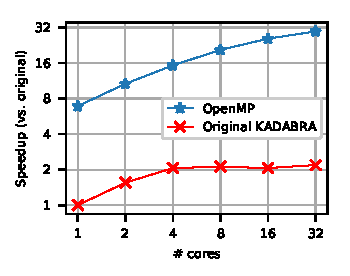
\includegraphics{sources/plots/betw-apx/original-vs-baseline.pdf}
\caption{Average speedup (preprocessing + ADS, geom.\ mean) of OpenMP baseline over
the original sequential implementation of \kadabra.}
\label{fig:betw-apx:original-vs-baseline}
\end{subfigure}\hfill
\begin{subfigure}[t]{.48\textwidth}
\centering
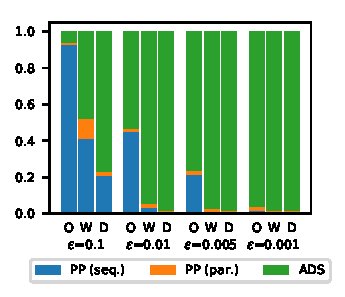
\includegraphics{sources/plots/betw-apx/time-breakdown.pdf}
\caption{Breakdown of sequential \kadabra running times into preprocessing and ADS
(in percent) on instances orkut-links~(O), wikipedia\_link\_de~(W), and
dimacs9-COL~(D)}
\label{fig:betw-apx:time-breakdown}
\end{subfigure}
\caption{Performance of OpenMP baseline.}
\end{figure}

In a first experiment, we compare our OpenMP baseline against the original
implementation of \kadabra (see \Cref{sec:betw-apx:first-attempts} for these two
approaches). We set the absolute approximation error to $\epsilon =
\numprint{0.01}$. The overall speedup (\ie both preprocessing and ADS) are
reported in \Cref{fig:betw-apx:original-vs-baseline}.
The results show that our OpenMP baseline outperforms the
original implementation considerably (by a factor of
$\onedigit{\adsSuDtVsOmp}\times$), even in a single-core setting.
%
This is mainly due to implementation tricks (see
\Cref{sec:betw-apx:kad-improvements}) and parameter tuning (as discussed in
\Cref{sec:betw-apx:balancing-costs}). Furthermore, for $32$ cores, our OpenMP
baseline performs $\onedigit{\overallSuOmpVsOriginal}\times$ better than the
original implementation of \kadabra\ -- or
$\onedigit{\adsSuOmpVsOriginal}\times$ if only the ADS phase is considered.
Hence, for the remaining experiments, we discard the original implementation as
a competitor and focus on the parallel speedup of our algorithms.

\subsection{Preprocessing and ADS Costs}
%
To understand the relation between the preprocessing and ADS phases of
\kadabra, we break down the running times of the OpenMP baseline
in \Cref{fig:betw-apx:time-breakdown}. In this plot, we present the fraction
of time that is spent on ADS on three exemplary instances and for different
values of $\epsilon$.
Especially if $\epsilon$ is small, the ADS running time dominates the overall
performance of the algorithm.
Thus, improving the scalability of the ADS phase is of critical importance.
For this reason, we neglect the preprocessing phase and only consider ADS when
comparing to our \localframe and \sharedframe algorithms.


\subsection{Parallel Speedup}
%
\begin{figure}[t]
\centering
\begin{subfigure}[t]{.48\textwidth}
\centering
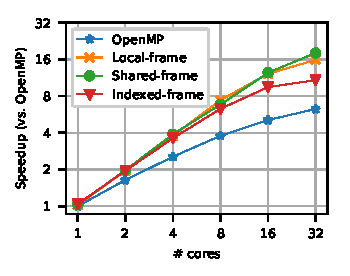
\includegraphics{sources/plots/betw-apx/parallel-speedup.pdf}
\caption{Average ADS speedup (geom.\ mean) of epoch-based
algorithms over sequential OpenMP baseline.}
\label{fig:betw-apx:parallel-speedup}
\end{subfigure}\hfill
\begin{subfigure}[t]{.48\textwidth}
\centering
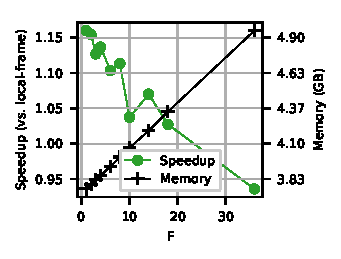
\includegraphics{sources/plots/betw-apx/time-memory.pdf}
\caption{Average ADS speedup (over 36-core \localframe, geom.\ mean)
and memory consumption of \sharedframe, depending on the number
of SFs.}
\label{fig:betw-apx:time-memory}
\end{subfigure}
\caption{Performance of epoch-based algorithms.}
\end{figure}

In \Cref{fig:betw-apx:parallel-speedup} we report the parallel
speedup of the ADS phase of our epoch-based algorithms
relative to the OpenMP baseline.
All algorithms are configured to check the stopping condition
after a fixed number of samples (see \Cref{sec:betw-apx:termination-latency}
for details). The number $F$ of SF pairs of \sharedframe
has been configured to $2$, which we found to be a good setting
for $T = 32$. On $32$ cores, \localframe and \sharedframe achieve
parallel speedups of $\onedigit{\adsParallelSuLf}\times$
and $\onedigit{\adsParallelSuSf}\times$; they both significantly
improve upon the OpenMP baseline, which can only
achieve a parallel speedup of $\onedigit{\adsParallelSuNaive}\times$
(\ie \localframe and \sharedframe are $\onedigit{\adsSuLfVsOmp}\times$
and $\onedigit{\adsSuSfVsOmp}\times$ faster, respectively;
they also outperform the original implementation by
factors of $\onedigit{\adsSuLfVsOriginal}\times$ and
$\onedigit{\adsSuSfVsOriginal}\times$, respectively).
%
The difference between \localframe and \sharedframe is insignificant
for lower numbers of cores; this is explained by the fact that the reduced
memory footprint of \sharedframe only improves performance once memory
bandwidth becomes a bottleneck. For the same reason, both algorithms
scale very well until $16$ cores; due to memory bandwidth limitations,
this nearly ideal scalability does not extend to $32$ cores.
This bandwidth issue is known to affect graph traversal algorithms
in general~\cite{DBLP:conf/icpp/BaderCF05,DBLP:journals/ppl/LumsdaineGHB07}.

\subsection{Indexed-frame Algorithm}
\label{sec:betw-apx:exp-indexed-frame}
%
The \indexedframe algorithm is not as fast as \localframe and \sharedframe on
the instances depicted in \Cref{fig:betw-apx:parallel-speedup}; it achieves a
parallel speedup of $\onedigit{\adsParallelSuDt}\times$ on $32$ cores. However,
it is still considerably faster than the OpenMP baseline (by a factor of
$\onedigit{\adsSuDtVsOmp}\times$). There are two reasons why the determinism of
\indexedframe is costly: \indexedframe has similar bandwidth requirements as
\localframe; however, it has to allocate more memory as SFs are buffered for
longer periods of time. On the other hand, even when enough samples are
collected, the stopping condition has to be checked on older samples first,
while \localframe and \sharedframe can just check the stopping condition on the
most recent sampling state.

\subsection{Impact of Parameter $F$}
%
In a final experiment, we evaluate the impact of the parameter $F$ of
\sharedframe on its performance. Note that this experiment also
demonstrates the difference in memory consumption of \sharedframe
($F \in \set{1, \ldots, T}$) and \localframe (equivalent to
$F = T$). \Cref{fig:betw-apx:time-memory} depicts the results.
%
The experiment is done with $36$ cores; hence, memory pressure
is even higher than in the previous experiments.
The plot demonstrates that, in this situation, minimizing the
memory bandwidth requirements at the expense of synchronization
overhead is a good strategy. Hence, for larger number of cores,
we can minimize memory footprint and maximize performance
at the same time.

\section{Related Work}
\label{sec:betw-apx:related-work}
%
\paragraph{ADS Algorithms}
%
Our parallelization strategy can be applied to arbitrary ADS algorithms. ADS
was first introduced by Lipton and Naughton to estimate the size of the
transitive closure of a digraph~\cite{DBLP:conf/vldb/LiptonN89}. It is used in
a variety of fields, \eg in statistical
learning~\cite{DBLP:conf/kdd/ProvostJO99}.
%
In the context of betweenness centrality, ADS has been used to approximate
distances between pairs of vertices of a graph~\cite{oktay2011distance}, to
approximate the $\betw(\cdot)$ value of the vertices in a
graph~\cite{DBLP:conf/waw/BaderKMM07,DBLP:conf/waw/BaderKMM07,DBLP:journals/tkdd/RiondatoU18},
and to approximate the betweenness centrality of a single
vertex~\cite{DBLP:journals/corr/abs-1810-10094}. An analogous strategy is
exploited by Mumtaz and Wang~\cite{DBLP:conf/cikm/MumtazW17} to find
approximate solutions to the group-betweenness maximization problem.

\paragraph{Betweenness Centrality Approximation Algorithms}
%
Regarding more general (\ie not necessarily ADS) algorithms
for $\betw(\cdot)$, a survey from Matta \etal~\cite{matta2019comparing}
provides a detailed overview of the state of the art.
The \rk~\cite{DBLP:journals/datamine/RiondatoK16} algorithm represents the
leading non-adaptive sampling algorithm for betweenness centrality approximation;
\kadabra was shown to be $100\times$ faster than \rk in undirected real-world
graphs, and $70\times$ faster thank \rk in directed graphs~\cite{DBLP:conf/esa/BorassiN16}
McLaughlin and Bader~\cite{DBLP:conf/sc/McLaughlinB14} introduced a work-efficient parallel
algorithm for betweenness centrality approximation, implemented for single- and multi-GPU
machines. Madduri \etal~\cite{DBLP:conf/ipps/MadduriEJBC09} presented a lock-free
parallel algorithms optimized for specific massively parallel non-x$86\_64$ architectures
to approximate or compute $\betw(\cdot)$ exactly in massive networks.
Unlike our approach, this lock-free algorithm parallelizes the collection of individual
samples and is thus only applicable to betweenness centrality and not to general
ADS algorithms. Additionally, according to the authors of~\cite{DBLP:conf/ipps/MadduriEJBC09}
this approach hits performance bottlenecks on x$86\_64$ even for $4$ cores.

\paragraph{Concurrent Data Structures}
%
The SFs used by our algorithms are concurrent data structures that enable us to minimize
the synchronization latencies in multi-threaded environments.
Devising concurrent (lock-free) data structures that scale over multiple cores is not
trivial and much effort has been devoted to this
goal~\cite{DBLP:conf/osdi/Boyd-WickizerCMPKMZ10,DBLP:journals/tpds/Michael04}.
A well-known solution is the Read-Copy-Update mechanism (RCU); it was introduced
to achieve high multi-core scalability on read-mostly data
structures~\cite{mckenney1998read}, and was leveraged by several
applications~\cite{DBLP:conf/podc/ArbelA14,DBLP:conf/asplos/ClementsKZ12}.
Concurrent hash tables are another popular example~\cite{DBLP:conf/sosp/DavidGT13}.

\section{Conclusions}
%
In this chapter, we observed that previous techniques to
parallelize ADS algorithms are insufficient to scale to large numbers of
threads. However, we found that significant speedups can be achieved by
employing adequate concurrent data structures. Using such data structures in
connection with our new epoch-based mechanism, we were able to devise parallel
ADS algorithms that, in our betweenness centrality case study, consistently
outperform the state of the art but also achieve different trade-offs between
synchronization costs, memory footprint, and determinism of the result.

Sampling-based strategies are used to estimate other centralities such as
closeness~\cite{DBLP:journals/ijbc/BrandesP07,DBLP:journals/jgaa/EppsteinW04},
group betweenness~\cite{DBLP:conf/ipps/MadduriEJBC09}, electrical
closeness~\cite{DBLP:conf/esa/AngrimanPGM20}, or (group-) forest
closeness~\cite{DBLP:conf/sdm/GrintenAPM21}. Hence, regarding future work, a
promising direction for our algorithms is to adapt them to approximate other
centrality measures beyond betweenness.

%%%%%%%%%%%%%%%%%%%%%%%%%%%%%%%%%%%%%%%%%%%%%%%%%%%%%%%%%%%%%%%%%%%%%%%%
\chapter{Approximation of the Diagonal of a Laplacian’s Pseudoinverse for Complex Network Analysis}
\label{ch:electrical-closeness}
% Labels: approximate, static, algebraic, parallel
%%%%%%%%%%%%%%%%%%%%%%%%%%%%%%%%%%%%%%%%%%%%%%%%%%%%%%%%%%%%%%%%%%%%%%%%

\section{Introduction}
\label{sec:el-clos:intro}
%
In this chapter, we address the problem of approximating electrical centrality
measures for the analysis of complex networks -- also known as
small-world networks, \ie graphs whose diameter is bounded by $\Oh(\log n)$,
see \Cref{sec:intro:methodology}.
The small-world feature is typical of many real-world
networks such as social networks, biological networks, information networks,
\etc~\cite{newman2018networks}. As described in \Cref{sec:centrality-measures},
many centrality measures exist, some of which are based on shortest paths (or
shortest-path distances) while others consider paths of arbitrary lengths.
Electrical centrality measures interpret the graph as an electrical
network~\cite{lovasz1993random} and thus fall in the latter category. Here we
consider two electrical centrality measures: electrical closeness
centrality ($\elclos$)~\cite{DBLP:conf/stacs/BrandesF05} -- \aka current-flow
closeness or information centrality~\cite{stephenson1989rethinking} -- and
forest closeness centrality ($\fclosp$)~\cite{DBLP:conf/icdm/JinBZ19}.

\paragraph{Electrical Closeness}
The electrical closeness of a vertex $u \in V$ (see
\Cref{eq:electrical-closeness}) is defined as the reciprocal of the average
effective resistance $\rdist(u, \cdot)$ from $u$ to all other
vertices.\footnote{We remark that effective resistance
has numerous applications well beyond its usage in electrical centrality measures -- cf.
Refs.~\cite{DBLP:conf/innovations/AlevALG18,DBLP:journals/siamrev/GhoshBS08}.}
The effective resistance between two vertices $u, v\in V$ can be computed by solving
the linear system $\Lapl\vect{x} = \cunit{u} - \cunit{v}$ for $\vect{x}$, where
$\cunit{z}$ is the canonical unit vector for vertex $z$. Then,
$\rdist(u, v) = \vect{x}[u] - \vect{x}[v]$.
It is well-known that $\Lapl$ does not have full rank and is thus not invertible.
Its Moore-Penrose pseudoinverse~\cite{DBLP:books/daglib/0086372} $\Linv$,
however, can be used to compute $\rdist(u, v)$ as shown in
\Cref{eq:eff-res-laplinv}.

A straightforward way to compute the electrical closeness of any vertex would
be to compute $\Linv$ which, without exploiting the structure of $\Lapl$,
\change{takes} in practice \change{cubic time in $n$}, cf. Ref.
\cite{DBLP:conf/cocoa/RanjanZB14}. Further, this strategy would require
$\change{\Theta(n^2)}$ memory since $\Linv$ is in general a dense matrix --
even for sparse $\Lapl$. Therefore, full (pseudo)inversion is clearly limited
to small inputs.

Conceptually similar to inversion would be to solve $\Theta(n)$ Laplacian linear systems.
Fewer linear systems suffice in applications with lower accuracy requirements:
the Johnson-Lindenstrauss Transform (JLT) combined with a fast Laplacian solver (such as
Ref.~\cite{DBLP:conf/stoc/CohenKMPPRX14}) achieve
a relative approximation guarantee by solving $\Oh(\log n /\epsilon^2)$
systems~\cite{DBLP:journals/siamcomp/SpielmanS11} in $\tilde{\Oh}(m\log^{1/2}
n \log (1/\epsilon))$ time each, where $\tilde{\Oh}(\cdot)$ hides a
$\Oh((\log\log n)^{3 + \delta})$ factor for $\delta > 0$.

As pointed out by Bozzo and Franceschet~\cite{DBLP:journals/socnet/BozzoF13},
the (only) relevant part of $\Linv$ for computing the electrical closeness is
its diagonal -- we will see that this is true for other electrical centrality
measures as well. Numerical methods for sampling-based approximation of the
diagonal of implicitly given matrices already exist~\cite{bekas2007estimator}.
Yet, for our purpose, they solve $\Oh(\log n /\epsilon^2)$ linear system as
well to obtain an $\epsilon$-approximation with high probability.
%
While Laplacian linear systems can be solved independently in parallel, their solution can
still be time-consuming in practice, in part due to high constant overheads hidden
in the $\Oh$-notation.


\paragraph{Forest Closeness}
Forest closeness (see \Cref{eq:forest-closeness}) is based on the forest distance,
a metric introduced by Chebotarev and Shamis~\cite{chebotarev2000forest}.
It is defined as closeness centrality where the shortest-path distance is replaced
by the forest distance.
In sociology, forest distances are shown to effectively capture sensitive relationship indices
such as social proximity and group cohesion~\cite{DBLP:journals/corr/abs-math-0602070}.
Hence, forest closeness has two main advantages over many other centrality
measures~\cite{DBLP:conf/icdm/JinBZ19}: (i) unlike electrical closeness, it can
handle disconnected graphs out of the box and, by considering not only shortest
paths, (ii) it has a high discriminative power.

Jin \etal~\cite{DBLP:conf/icdm/JinBZ19} provided an approximation algorithm for
forest closeness centrality with nearly-linear time complexity. Similarly to
the aforementioned strategy for electrical closeness, their algorithm uses the
JLT and fast linear solvers; it is, however, still time-consuming. For example,
in their experimental study~\cite{DBLP:conf/icdm/JinBZ19}, graphs with
$\approx$ 1M to $\approx$ 2-3M edges require more than $\numprint{2.3}$ to
$\numprint{4.7}$ \emph{hours} for a reasonably accurate ranking. Clearly, this
hardly scales to larger graphs with \change{more than a few million edges}.

As already realized by Chebotarev and Shamis~\cite{chebotarev2000forest},
forest distance is closely connected to effective resistance. In particular, as
we describe in \Cref{sec:el-clos:forest-clos-extension}, any algorithm that
computes the electrical closeness can easily be adapted to compute the forest
closeness with just an additional linear-time overhead.

\subsection{Related Work}
\paragraph{Solving Laplacian Systems}
As mentioned above, a straightforward approach to compute electrical closeness
is to compute $\Linv$ by solving a number of Laplacian systems.
Brandes and Fleischer~\cite{DBLP:conf/stacs/BrandesF05} compute electrical closeness
from the solution of $n$ linear systems using Conjugate Gradient (CG) in $\Oh(mn\sqrt{\kappa})$,
where $\kappa$ is the condition number of the appropriately preconditioned Laplacian
matrix.\footnote{Brandes and Fleischer provide a rough estimate of $\kappa$
as $\Theta(n)$, leading to a total time of $\Oh(mn^{\numprint{1.5}})$.}
%
Later, Spielman and Srivastava~\cite{DBLP:journals/siamcomp/SpielmanS11}
proposed an approximation algorithm to compute effective resistance distances.
The main components of the algorithm are (i) a dimension reduction with
JLT~\cite{johnson1984extensions} and (ii) the use of a fast
Laplacian solver for $\Oh(\log n/\epsilon^2)$ Laplacian systems. The algorithm
approximates effective resistance values for all edges with a factor of $(1 \pm
\epsilon)$ in $\Oh(I(n, m)\log n/\epsilon^2)$ time, where $I(n, m)$ is the
running time of the Laplacian solver, assuming that the solution of the
Laplacian systems is exact. With an approximate Laplacian solution, the algorithm
yields a $(1 + \epsilon)^2$-approximation. Significant progress in the development
of Laplacian solvers with theoretical guarantees~\cite{DBLP:conf/stoc/CohenKMPPRX14,
DBLP:conf/stoc/KelnerOSZ13,DBLP:conf/focs/KoutisMP11,DBLP:journals/siamcomp/KoutisMP14,
DBLP:conf/stoc/KyngLPSS16}
has resulted in the currently best one running in $\Oh(m\log^{1/2}n \log
1/\epsilon)$ time (up to polylogarithmic
factors)~\cite{DBLP:conf/stoc/CohenKMPPRX14}.
%
Parallel algorithms for solving linear systems on the more general SDD matrices
also exist in the
literature~\cite{DBLP:conf/spaa/BlellochGKMPT11,DBLP:conf/stoc/PengS14}. To
date, the fastest algorithms for electrical closeness and spanning edge
centrality\footnote{The spanning edge centrality of an edge $e$ in a graph $G$
is defined as the number of spanning trees in $G$ that contain $e$ and it
is equivalent to the effective resistance of
$e$~\cite{DBLP:conf/www/MavroforakisGKT15}.}
extend the idea of Spielman and
Srivastava~\cite{DBLP:conf/siamcsc/BergaminiWLM16,
DBLP:conf/ijcai/HayashiAY16,DBLP:conf/www/MavroforakisGKT15}
-- similar ideas are also used for centrality measures based on the Kirchhoff
index, see \Cref{sec:el-clos:generalizations}. Since theoretical Laplacian
solvers rely on heavily graph-theoretic machinery such as low-stretch spanning
trees, multigrid
solvers~\cite{DBLP:conf/siamcsc/BergaminiWLM16,
DBLP:conf/isvc/KoutisMT09,DBLP:journals/siamsc/LivneB12}
are used in practice instead.

\paragraph{Diagonal Estimation}
Recall that only the diagonal of $\Linv$ [or of $\Fmat$, resp.] is enough to
compute the electrical closeness -- or, in case of the Kirchhoff index, only
the sum of $\diag{\Linv}$, \ie the trace $\tr{\Linv}$ is required -- [or the
forest closeness].
%
Algorithms that approximate the diagonal (or the trace) of matrices that are
only implicitly available often use iterative
methods~\cite{DBLP:journals/na/SidjeS11}, sparse direct
methods~\cite{DBLP:journals/siamsc/AmestoyDLR15,DBLP:journals/pc/Jacquelin0018},
Monte Carlo~\cite{hutchinson1989stochastic} or deterministic probing
techniques~\cite{bekas2007estimator,bekas2007estimator}.
%
A popular approach is the standard Monte-Carlo method for the trace of a matrix \mat{B}, due to
Hutchinson~\cite{hutchinson1989stochastic}. The idea is to estimate the trace of \mat{B} by
observing the action of \mat{B} (in terms of matrix-vector products) on a sufficiently large
sample of random vectors. In our case, this would require to solve a large number of Laplacian
linear systems with random vectors as right-hand sides. Avron and Toledo~\cite{DBLP:journals/jacm/AvronT11}
proved that the method requires $\Oh(\log n /\epsilon^2)$ samples to achieve a maximum error
of $\epsilon$ with probability at least $1 - \delta$. The approach from Hutchinson~\cite{hutchinson1989stochastic}
was extended by Bekas \etal~\cite{bekas2007estimator} for estimating \diag{\mat{B}}.
Finally, Barthelem\'e \etal~\cite{barthelme2019estimating} proposed a combinatorial algorithm to
approximate the trace (not the diagonal) of the inverse of a matrix closely related to the Laplacian.
Their algorithm can be seen as a special case of our algorithm in a situation where a universal
vertex exists (\ie a vertex connected to all the other vertices of the graph).

\subsection{Contribution and Outline}
We introduce a new algorithm for approximating \diag{\Linv} of a Laplacian matrix \Lapl
that corresponds to weighted undirected graphs (\Cref{sec:el-clos:apx-algo}). Our main technique
is the approximation of effective resistances between a pivot vertex $u\in V$ and
all other vertices of $G$.
It is based on sampling uniform (= random) spanning trees (USTs).
The resulting algorithm is highly parallel and (almost) purely combinatorial -- it relies on the
connection between Laplacian linear systems, effective resistances, and USTs.
Because effective resistance also plays a major role in \emph{normalized
random-walk betweenness}~\cite{DBLP:conf/complexnetworks/NarayanS18}
and \emph{Kirchhoff index centrality}~\cite{DBLP:conf/soda/LiZ18}, in this
chapter we consider these measures as well.

For small-world graphs, our algorithm obtains an absolute
$\pm\epsilon$-approximation guarantee with high probability in (sequential)
time $\Oh(m\log^4n\cdot\epsilon^{-2})$. In particular, compared to the fastest
theoretical Laplacian solvers in connection with JLT, our approach is off by
only a polylogarithmic factor. More importantly from a practical perspective,
after some algorithm engineering (\Cref{sec:el-clos:eng}), our algorithm
performs much better than the state of the art, already in our sequential
experiments (\Cref{sec:el-clos:exp-el-clos}): (i) it is much faster and more
memory-efficient, (ii) it yields a maximum absolute error that is one order of
magnitude lower, and (iii) results in a more accurate complete centrality
ranking of elements of \diag{\Linv}. Furthermore, due to good parallel
speedups, we can even compute a reasonably accurate diagonal of $\Linv$ on a
small-scale cluster with 16 compute nodes in less than 8 minutes for a graph
with $\approx\numprint{13.6}$M vertices and $\approx\numprint{334.6}$M edges.

Concerning forest closeness centrality, we adapt our UST sampling technique to
approximate $\fclosp(\cdot)$ for each vertex in the graph. Our experiments
in \Cref{sec:el-clos:exp-forest} show that our algorithm for ranking individual
vertices is always substantially faster than the state of the
art~\cite{DBLP:conf/icdm/JinBZ19}; specifically, for sufficiently large
networks and in a sequential setting, it is one to two orders of magnitude faster
while often achieving better accuracy.
Our new algorithm can rank all vertices in
networks with up to $\numprint{334.6}$M edges with reasonable accuracy in less
than 20 minutes if executed in an MPI-parallel setting on a small-scale cluster
with 16 compute nodes.

\bibnotes{
The algorithms for approximating $\diag{\Linv}$ were published in the
Proceedings of the \emph{Twenty-Eighth Annual European Symposium on Algorithms
(ESA 2020)} while the approximation algorithms for forest closeness were
presented in the Proceedings of the \emph{Twenty-First SIAM International
Conference on Data Mining (SDM 2021)}. Among those presented in this chapter,
my contributions involve the implementation of all presented algorithms and
carrying out the experiments.
The rest is joint work with Maria Predari, Alexander van der Grinten,
and Henning Meyerhenke. Proofs to which I did not contribute are omitted and
can be found in in the original
papers~\cite{DBLP:conf/esa/AngrimanPGM20,DBLP:conf/sdm/GrintenAPM21}.}

\section{Preliminaries}
\label{sec:el-clos:prelim}

As input we consider simple undirected graphs $G = (V, E, w)$ with
non-negative edge weights -- for electrical closeness, we also assume that $G$ is connected.
For the complexity analysis, we usually assume that $\diam(G) \in \Oh(\log n)$, but our
algorithm works correctly even without this assumption.

\paragraph{Graphs as Electrical Networks}
Recall our notation for electrical networks provided in
\Cref{sec:prelim-resistance-distance}. We interpret $G$ as an electrical
network in which every edge $e\in E$ represents a resistor with resistance
$1/w(e)$.
The effective resistance between two vertices $u,v\in V$, denoted by $\rdist(u, v)$,
is defined as the potential difference between $u$ and $v$ when a unit of current
is injected into $G$ at $u$ and extracted at $v$ -- see \Cref{def:resistance-distance}.
To compute $\rdist(u, v)$, we can either use the Moore-Penrose pseudoinverse as shown
in \Cref{eq:eff-res-laplinv}:
%
\begin{equation}
\label{eq:el-clos:eff-res}
\rdist(u, v) = (\cunit{u} - \cunit{v})^\top\Linv(\cunit{u} - \cunit{v}) =
\Linv[u,u] - 2\Linv[u,v] + \Linv[v,v],
\end{equation}
%
or, equivalently, $\rdist(u, v) = \vect{x}[u] - \vect{x}[v]$, where $\vect{x}$
is the solution vector of the Laplacian linear system $\Lapl\vect{x} =
\cunit{u} - \cunit{v}$.
Recall from \Cref{eq:laplinv} that $\Linv$ can be expressed as:
%
\[
\Linv = \roundb{\Lapl + \frac1n \Ones}^{-1} - \frac1n \Ones,
\]
%
where $\Ones$ is the $n\times n$-matrix with all entries being 1.
Also, note that the effective resistance between the endpoints of an edge $e\in E$
equals the probability that $e$ is an edge in a UST, \ie a spanning tree selected
uniformly at random among all spanning trees of $G$, cf.~\cite[Ch. II]{DBLP:books/daglib/0009415}.

\paragraph{Electrical Closeness}
The combinatorial counterpart of electrical closeness (\Cref{eq:def:closeness})
is based on shortest-path distances: $\clos(u) := (n - 1) / \farn(u)$, where the
denominator is the \emph{combinatorial farness} of $u$:
%
\begin{equation}
\label{eq:comb-farness}
    \farn(u) := \sum_{v \in V \setminus \set{u}} d(u, v).
\end{equation}

Electrical farness ($\elfarn$) is defined analogously to combinatorial
farness -- shortest-path distance in \Cref{eq:comb-farness} is replaced by
effective resistance $\rdist(u, v)$. Both combinatorial and electrical farness
are not defined for disconnected graphs due to infinite distances. A solution
to this issue already exists: Lin's index~\cite{lin1976foundations} is a
generalization of combinatorial closeness to disconnected graphs and can easily
be adapted to the electrical case as well. Thus, our assumption of $G$ being
connected is no limitation.

\paragraph{Normalized Random-Walk Betweenness}
Contrary to classical betweenness, which is based on shortest paths (see
\Cref{eq:def:betweenness}), normalized random-walk betweenness ($\nrwb(\cdot)$, abbreviated with NRWB)
considers random walks~\cite{DBLP:conf/complexnetworks/NarayanS18}. More
precisely, let $s \in V$ be a source vertex, $t \in V\setminus\set{s}$ be a destination vertex,
and assume we are trying to obtain the NRWB of some other vertex $u \in V\setminus\set{s, t}$;
$\nrwb(u)$ counts the fraction $\mu_{s, t}(u)$ of random walks starting from
$s$ passing through $u$ only once.
To compute $\nrwb(u)$, $\mu_{s, t}(u)$ is averaged over all $s\in V$ and
$t \in V\setminus \set{s}$:
%
\[
\nrwb(u) = \frac{1}{n(n - 1)}
\sum_{\substack{s,t \in V \setminus \set{u}\\s\neq t}}\roundb{\mu_{s, t}(u) + (n - 1)}.
\]

Narayan and Saniee~\cite{DBLP:conf/complexnetworks/NarayanS18} obtain a
closed-form expression of NRWB:

\begin{equation}
\label{eq:def:nrwb}
\nrwb(u) = \frac{1}{n} + \frac{1}{n - 1}\sum_{t \in V \setminus \set{u}}
\frac{\mat{M}^{-1}[t, t] - \mat{M}^{-1}[t, u]}{\mat{M}^{-1}[t, t] + \mat{M}^{-1}[u, u] - 2\mat{M}^{-1}[t, u]},
\end{equation}
%
where $\mat{M} := \Lapl + \mat{P}$, with $\mat{P}$ the projection operator onto
the zero eigenvector of the Laplacian \Lapl, \ie $\mat{P}[i, j] = 1/n$. In
\Cref{sec:el-clos:generalizations} (\Cref{lemma:el-clos:simpler-nrwb}), we show
how to simplify this expression and how our algorithm can be adapted to NRWB.

\paragraph{Kirchhoff Index and Related Centrality Measures}
The Kirchhoff index $\kidx(G)$~\cite{ellens2011effective,klein1993resistance}
-- \aka (effective) graph resistance -- is the sum of the effective resistance
distances over all pairs of vertices in $G$ and is an important measure for
network robustness. The Kirchhoff index is often computed via the closed-form
expression $\kidx(G) = n\ \tr{\Linv}$~\cite{klein1993resistance}.

Li and Zhang~\cite{DBLP:conf/soda/LiZ18} adapted the Kirchhoff index to obtain
two new \emph{edge} centrality measures for $e \in E$. Let $G
\textbackslash_{\theta}e$ be the graph obtained by deactivating edge $e$, \ie
decreasing its weight of $e$ from $w(e)$ to $\theta w(e)$ for some small
$\theta \in (0, 1/2]$, and let $\Lapl\textbackslash_{\theta}e$ be the Laplacian
matrix of $G\textbackslash_{\theta}e$. The new measures are:
\begin{itemize}
    \item $c_{\theta}(e) := n\ \tr{\Linv\textbackslash_{\theta}e}$, \ie the
        Kirchhoff index of the graph $G\textbackslash_{\theta}e$;
    \item $c_{\theta}^{\Delta}(e) := c_{\theta}(e) - \kidx(G)$ \ie the
        difference between the Kirchhoff indices of graph
        $G\textbackslash_{\theta}e$ and $G$.
\end{itemize}

To calculate the Kirchhoff edge centralities, Li and
Zhang~\cite{DBLP:conf/soda/LiZ18} use techniques such as partial Cholesky
factorization~\cite{DBLP:conf/focs/KyngS16}, fast Laplacian solvers, and the
Hutchinson estimator. For $c_{\theta}^{\Delta}(e)$, which is the more
interesting measure in our context, they propose an $\epsilon$-approximation
algorithm that approximates $c_{\theta}^{\Delta}(e)$ for all edges in
$\Oh(m\epsilon^{-2}\theta^{-2}\log^{\numprint{2.5}}n\log(1/\epsilon))$ time --
up to polylogarithmic factors. The algorithm uses the Sherman-Morrison
formula~\cite{sherman1950adjustment}, which gives a fractional expression of
$\roundb{\Linv\textbackslash_{\theta}e - \Linv}$. The numerator is approximated
by the Johnson-Lindenstrauss lemma and the denominator by effective resistance
estimates for all edges.

Following the definition of $\kidx(G)$, it is easy to see that
an algorithm that approximates $\diag{\Linv}$ also
approximates the Kirchhoff index.

\paragraph{Forest Closeness}
Similarly to its combinatorial counterpart, forest closeness is inversely
proportional to \emph{forest farness}, \ie the sum of the forest distances
from a vertex to all other vertices. The forest distance between two vertices $u,v\in V$
(see \Cref{def:forest-distance} in \Cref{sec:prelim:forest-distance}) is a
one-parametric metric $\fdistp(u, v)$ defined in terms of the forest matrix
$\Fmatp := (\alpha\Lapl + \Ident)^{-1}$~\cite{chebotarev2000forest}:
%
\begin{equation}
\label{eq:el-clos:f-dist}
\fdistp(u, v) := (\cunit{u} - \cunit{v})^\top \Fmatp (\cunit{u} - \cunit{v}) =
\Fmatp[u,u] - 2\Fmatp[u,v] + \Fmatp[v,v].
\end{equation}

Hence, the forest farness and the forest closeness of a vertex $u$ are defined as:
%
\begin{equation}
\label{eq:el-clos:forest-clos}
\ffarnp(u) := \sum_{v \in V \setminus \set{u}}\fdistp(u)\quad \text{and}\quad
\fclosp(u) := \frac{n}{\ffarnp(u)},
\end{equation}
%
respectively. Non-parametric variants of forest closeness fix $\alpha$ to
1~\cite{DBLP:journals/corr/abs-math-0602073}. To simplify our notation, in the
following we omit $\alpha$ when clear from the context. As we explain in more
detail in \Cref{sec:el-clos:forest-clos-extension}, a close connection between
forest closeness and electrical closeness allows us to easily adapt our
algorithm for electrical closeness approximation to forest closeness.

\section{Approximation Algorithm for Electrical Closeness}
\label{sec:el-clos:apx-algo}
\subsection{Overview}
In order to compute the electrical closeness for all vertices in $V$, the main challenge
is obviously to compute their electrical farness $\elfarn(\cdot)$. Recall from
\Cref{sec:el-clos:intro} that the diagonal of $\Linv$ is sufficient to compute
$\elfarn(\cdot)$ for all vertices simultaneously
-- comp. Ref.~\cite[Eq. (15)]{DBLP:journals/socnet/BozzoF13}) with a slightly different
definition of electrical closeness.
This follows from \Cref{eq:el-clos:eff-res} and from the fact that each row/column in
\Linv sums to 0:
%
\[
\elfarn(u) :=
\sum_{v \in V \setminus \set{u}}\rdist(u, v) = n \Linv[u, u] + \tr{\Linv} - 2\sum_{v\in V}\Linv[u, v] =
n\Linv[u, u] + \tr{\Linv},
\]
%
since $\tr{\cdot}$ is the sum over the diagonal entries.
We are interested in an approximation of $\diag{\Linv}$, since we do not necessarily
need exact values for our particular applications. To this end, we propose an approximation
algorithm for which we give a rough overview first.
Our algorithm works best for small-world networks -- thus, we focus on this important
input class. Let $G$ be unweighted for now; we discuss the extension to weighted graphs
in \Cref{sec:el-clos:generalizations}.

\begin{enumerate}
\item Select\footnote{As we will see later on, one can improve the empirical running time
when $u$ is not chosen arbitrarily, but so as to have a low eccentricity. The correctness
and the asymptotic time complexity of the algorithm are not affected by the selection, though.}
a pivot vertex $u \in V$ and solve the linear system $\Lapl\vect{x} = \cunit{u} - \frac{1}{n}\ones$,
(recall that $\ones = (1, \ldots, 1)^\top$).
Out of all solutions \vect{x}, we want the one such that $\vect{x} \perp \ones$,
since this unique normalized solution is equal to $\Linv[:, u]$, \ie the column of
\Linv corresponding to $u$ -- see Ref.~\cite[pp. 6-7]{van2017pseudoinverse}.

\item As a direct consequence from \Cref{eq:el-clos:eff-res}, the diagonal entries $\Linv[v, v]$
for all $v\in V\setminus\set{u}$ can be computed as:
%
\[\Linv[v, v] = \rdist(u, v) - \Linv[u, u] + 2\Linv[v, u].\]

\item It remains to approximate these $n - 1$ effective resistance values $\rdist(u, \cdot)$.
To do so, we employ Kirchhoff's theorem, which connects electrical flows with spanning
trees~\cite[Ch. II]{DBLP:books/daglib/0009415}. Let $N$ be the total number of spanning trees
of $G$ and let $N_{s, t}(a, b)$ be the number of spanning trees in which the unique from $s$
to $t$ traverses the edge $\set{a, b}$ \emph{in the direction from} $a$ \emph{to} $b$.
Further, recall from \Cref{sec:prelim-resistance-distance} that $i(a, b)$ denotes the amount of
electrical current that flows from $a$ to $b$.

\begin{theorem}[Kirchhoff, comp.~\cite{DBLP:books/daglib/0009415}]
\label{theo:el-clos:kirchhoff}
Let $i(a, b) := (N_{s, t}(a, b) - N_{s, t}(b, a)) / N$. Distribute the current
flows on the edges of $G$ by sending a current of size $i(a, b)$ from $a$ to
$b$ for every edge $\set{a, b}$. Then there is a total current of size 1 from
$s$ to $t$ satisfying Kirchhoff's laws.
\end{theorem}

As a result of \Cref{theo:el-clos:kirchhoff}, the effective resistance between $s$ and $t$
is the potential difference between $s$ and $t$ induced by the current-flow given by $i$.
\change{Conversely}, since the current flow is induced by potential differences
(Ohm's law), one simply has to add the currents on a path from $s$ to $t$ to
compute $\rdist(s, t)$ -- see \Cref{eq:el-clos:eff-res-path} in
\Cref{sec:el-clos:eff-res-ust}. Actually, as a proxy for the current flows, we
use the (approximate) $N(\cdot)$-values mentioned in
\Cref{theo:el-clos:kirchhoff}.

\item For large graphs, it is impractical to compute the exact values for $N$
(\eg by Kirchhoff's matrix-tree theorem~\cite{DBLP:books/daglib/0037866},
which would require the determinant or all eigenvalues of \Linv) or
$N(\cdot)$. Instead, we obtain approximations of the desired values via sampling:
we sample a number uniform spanning trees and determine the $N(\cdot)$-values by
aggregation over the sampled trees. This approach provides a probabilistic absolute
approximation guarantee.
\end{enumerate}

Note that Steps 2-4 of the algorithm are entirely combinatorial. Step 1 may or may not be
combinatorial, depending on the Laplacian solver used. Corresponding implementation choices
are discussed in \Cref{sec:el-clos:eng}.

\begin{algorithm}[t]
\footnotesize
\setstretch{1}
\caption{\footnotesize Approximation algorithm for $\diag{\Linv}$.}
\label{algo:linv-diag-apx}
\textbf{Input:} Undirected graph $G = (V, E, w)$, pivot $u \in V$, error bound $\epsilon > 0$, probability $\delta\in (0, 1)$\\
\textbf{Output:} $\diag{\Linvapx}$, \ie an $(\epsilon, \delta)$-approximation of $\diag{\Linv}$

\begin{algorithmic}[1]
\State$\rdistapx(u, v) \gets 0\ \forall v \in V\setminus\set{u}$\Comment{$\Oh(n)$}\label{line:linv-diag-apx:rdist-init}
\State Pick a constant $\kappa\in(0, 1)$ arbitrarily
\State$\eta \gets \frac{\kappa\epsilon}{3\sqrt{mn\log n}\ \diam(G)}$\label{line:linv-diag-apx:eta}
\State Compute the BFS tree $B_u$ of $G$ with root $u$\Comment{$\Oh(n + m)$}
\label{line:linv-diag-apx:bu}
\State$\tau \gets \ecc(u)^2\cdot\ceil{\frac{\log(2m/\delta)}{2(1 - \kappa)^2\epsilon^2}}$\Comment{$\Oh(1)$}
\label{line:linv-diag-apx:tau}
\For{$j \gets 1$ \textbf{to} $\tau$}\label{line:linv-diag-apx:for-tau}
\State Sample UST $T_i$ of $G$ with root $u$\Comment{$\Oh(m\log n)$}
\State$\rdistapx(u, \cdot) \gets\textsc{Aggregate}(T_i, \rdistapx(u, \cdot), B_u)$\Comment{$\Oh(n\log n)$, see \Cref{algo:ust-aggregation}}
\EndFor\label{line:linv-diag-apx:end-ust-loop}
\State Solve $\Lapl\vect{x} = \cunit{u} - \frac{1}{n}\ones$ for \vect{x} with accuracy $\eta$
\Comment{$\tilde{\Oh}(m \log^{1/2}n \log (1 / \eta))$}\label{line:linv-diag-apx:solve}
\State$\Linvapx[u, u] \gets \vect{x}[u]$
\For{$v \in V\setminus\set{u}$}\Comment{Overall: $\Oh(n)$}
\State$\Linvapx[v, v] \gets \rdistapx(u, v)/\tau - \vect{x}[u] + 2\vect{x}[v]$\label{line:linv-diag-apx:update-linvapx}
\EndFor
\State\Return$\diag{\Linvapx}$
\end{algorithmic}
\end{algorithm}


\paragraph{Overall Algorithm}
\Cref{algo:linv-diag-apx} shows the pseudocode of our algorithm. The pivot vertex $u$ is already
received as an input parameter. \Crefrange{line:linv-diag-apx:rdist-init}{line:linv-diag-apx:end-ust-loop}
approximate the effective resistances $\rdist(u, \cdot)$. To do so,
\Crefrange{line:linv-diag-apx:rdist-init}{line:linv-diag-apx:tau} perform initializations:
first the estimate of the effective resistance $\rdistapx(u, v)$ is set to 0 for all vertices $v \in V$.
Then, the accuracy $\eta$ of the linear solver is computed so as to ensure an absolute
$\epsilon$-approximation for the whole algorithm. A BFS is performed from $u$ in order to compute
shortest paths from $u$ to all other vertices (more details in \Cref{sec:el-clos:eff-res-ust}).
The sample size $\tau$ depends on the parameters $\epsilon$ and $\delta$, among others.

The first \texttt{for}-loop in \Cref{line:linv-diag-apx:for-tau} performs the actual sampling
and aggregation of the USTs -- the latter with \Cref{algo:ust-aggregation}.
Afterwards, \Crefrange{line:linv-diag-apx:solve}{line:linv-diag-apx:update-linvapx}
fill the $u$-th column and the diagonal of \Linv -- to the desired accuracy.

\begin{remark}
Note that, due to the fact that Laplacian linear solvers provide a \emph{relative}
error guarantee (and not an absolute $\pm\epsilon$ guarantee), the (relative)
accuracy $\eta$ for the initial Laplacian linear system
(\Cref{line:linv-diag-apx:eta,line:linv-diag-apx:solve}) depends in a non-trivial way
on our guaranteed absolute error $\epsilon$. For details, see
\cite[Appendix A.4]{DBLP:conf/esa/AngrimanPGM20}.
\end{remark}

We also remark that the value of the constant $\kappa$ does not affect the
asymptotic running time (nor the correctness) of the algorithm.
However, it does affect the empirical running time by controlling which fraction
of the error budget is invested into solving the initial linear system vs. UST sampling.

In the reminder of \Cref{sec:el-clos:apx-algo}, we describe more in detail the
components and properties of \Cref{algo:linv-diag-apx}.

\subsection{Effective Resistance Approximation by UST Sampling}
\label{sec:el-clos:eff-res-ust}
Extending and generalizing work by Hayashi \etal~\cite{DBLP:conf/ijcai/HayashiAY16} on spanning
edge centrality, our main idea is to compute a sufficiently large sample of USTs and to aggregate
the $N(\cdot)$-values of the edges in those USTs.
Recall that, given an electrical flow with source $u$ and sink $v$, the effective resistance
between $u$ and $v$ equals the difference $\vect{x}[u] - \vect{x}[v]$, where \vect{x} is the solution
vector of the Laplacian linear system $\Lapl\vect{x} = \cunit{u} - \cunit{v}$. Since \vect{x}
is a potential and the electrical flow $i$ flows from its difference, $\rdist(u, v)$ can be computed
given \emph{any} path $(u = v_0, v_1, \ldots, v_{\ell - 1}, v_{\ell} = v)$ as:

\begin{equation}
\label{eq:el-clos:eff-res-path}
\rdist(u, v) = \sum_{j = 0}^{\ell - 1}i(v_j, v_{j + 1}) =
\frac{1}{N}\sum_{j = 0}^{\ell - 1}\roundb{N_{u, v}(v_j, v_{j + 1}) - N_{u, v}(v_{j + 1}, v_j)}.
\end{equation}

Recall that the sign of the current flow changes if we traverse an edge against the flow direction.
This is reflected by the second summand of \Cref{eq:el-clos:eff-res-path}. Since we can choose any path
from $u$ to $v$, for efficiency reasons we use \emph{one shortest} path $P_{u, v}$ per vertex
$v \in V\setminus\set{u}$.
We compute these paths with one breadth-first search (BFS) with root $u$, resulting in a
tree $B_u$ whose edges are considered implicitly directed from the root to the leaves.
For each vertex $v \in V \setminus\set{u}$, we maintain an estimate $\rdistapx(u, v)$ of
$\rdist(u, v)$, which is initially set to 0 for all $v$. After all USTs have
been sampled and processed, we divide all $\rdistapx(u, \cdot)$ by $\tau$, the number of sampled
trees -- \ie $\tau$ takes the role of $N$ in \Cref{eq:el-clos:eff-res-path}.

\paragraph{Sampling USTs}
In total, we sample $\tau$ USTs, where $\tau$ depends on the desired approximation guarantee and
is determined later. The choice of the UST algorithm depends on the input: for general graphs,
the algorithm by Shild~\cite{DBLP:conf/stoc/Schild18} with time complexity $\Oh(m^{1 + o(1)})$
is the fastest. Among others, it uses a sophisticated shortcutting techniques using fast Laplacian
solvers to speed up the classical
Aldous-Broder~\cite{DBLP:journals/siamdm/Aldous90,DBLP:conf/focs/Broder89}
algorithm. For unweighted small-world graphs, however, Wilson's~\cite{DBLP:conf/stoc/Wilson96}
simple algorithm using loop-erased
random walks takes $\Oh(m\log n)$ time, as we outline in the following. Thus, for our class of
inputs, Wilson's algorithm is preferred.

\paragraph{Wilson's UST Algorithm}
Given a path $P$, its loop erasure is a simple path created by removing all cycles of $P$
in chronological order. Wilson's algorithm grows a sequence of sub-trees of $G$, in our case
starting with $u$ as root of $T$. Let $M = \set{v_1, \ldots, v_{n - 1}}$ be an enumeration of
$V\setminus\set{u}$. Following the order in $M$, a random walk starts from every unvisited $v_i$,
until it reaches (some vertex in) $T$ and its loop erasure is added to $T$.

\begin{proposition}[\cite{DBLP:conf/stoc/Wilson96} comp.~\cite{DBLP:conf/ijcai/HayashiAY16}]
\label{prop:el-clos:wilson}
For a connected and unweighted undirected graph $G = (V, E)$ and a vertex $u \in V$, Wilson's
algorithm samples a UST of $G$ with root $u$. The expected running time is the mean hitting
time of $G$, $\sum_{v \in V\setminus\set{u}}\phi_G(v)\ctg(v, u)$, where $\phi_G(v)$ is the
probability that a random walk stays at $v$ in its stationary distribution and where
$\ctg(v, u)$ is the commute time between $v$ and $u$.
\end{proposition}

\begin{lemma}[\cite{DBLP:conf/sdm/GrintenAPM21}]
Let $G$ be as in \Cref{prop:el-clos:wilson}. Its mean hitting time can be rewritten as
$\sum_{v \in V \setminus\set{u}}\deg(v)\cdot\rdist(u, v)$, which is $\Oh(\ecc(u)\cdot m)$.
In small-world graphs, this is $\Oh(m\log n)$.
\end{lemma}

\paragraph{Data Structures}
When computing the contribution of a UST $T$ to $N(\cdot)$, we need to update
for each edge $e = (a, b) \in E(T)$ its contribution to $N_{u, v}(a, b)$ and
$N_{u, v}(b, a)$, respectively -- for exactly every vertex $v$ for which $(a,
b)$ [or $(b, a)$] lies on $P_{u, v}$. Hence, the algorithm that aggregates the
contribution of UST $T$ to $\rdistapx(u, \cdot)$ needs to traverse $P_{u, v}$
for each vertex $v \in V$. To this end, we represent the BFS tree $B_u$ as an
array of parent pointers for each vertex $v \in V$. On the other hand, the tree
$T$ can conveniently be represented by storing a child and a sibling for each
vertex $v \in V$. Compared to other representations (\eg adjacency lists), this
data structure can be constructed and traversed with low constant overhead.

\paragraph{Tree Aggregation}
After constructing a UST $T$, we process it to update the intermediate
effective resistance values $\rdistapx(u, \cdot)$. Note that we can discard $T$
afterwards as we do not need to store the full sample, which has a positive effect
on the memory footprint of our algorithm.
The aggregation algorithm is shown in \Cref{algo:ust-aggregation}.
Recall that we need to determine for which vertex $v$ and each edge $(a, b)\in P_{u, v}$,
whether $(a, b)$ or $(b, a)$ occurs on the unique $u$-$v$ path in $T$. To simplify this
test, we root $T$ at $u$; hence, it is enough to check if $(a, b)$ [or $(b, a)$]
appears above $v$ in $T$. For general graphs, such a test still incurs quadratic
overhead in running time -- in particular, the number of vertex-edge pairs that
need to be considered is $f(u) = \sum_{v \in V \setminus\set{u}}|P_{u, v}| \in \Oh(n^2)$.
We remark that, perhaps surprisingly, a bottom-up traversal of $T$ does not improve on
this, either; it is similarly difficult to determine all $\rdistapx(u, v)$
that a given $(a, b)\in E(T)$ contributes to -- those $v$ form an arbitrary subset of
descendants of $b$ in $T$. However, we can exploit the fact that, on small-world networks,
the depth of $B_u$ can be controlled, \ie $f(u)$ is sub-quadratic. To accelerate the test,
we first compute a DFS data structure for $T$, \ie we determine discovery and finish
timestamps for all vertices in $V$, respectively (\Cref{line:ust-agg:dfs}).
For an arbitrary $v \in V$ and $(a, b) \in V \times V$, this data structure allows us to
answer in constant time (i) whether either $(a, b)$ or $(b, a)$ is in $T$ and (ii)
if $(a, b) \in E(T)$, whether $v$ appears below $(a, b)$ in $T$.
Finally, the first \texttt{for}-loop iterates over all $v\in V\change{\setminus\set{u}}$
while the second
\texttt{for}-loop iterates over all $e = (a, b) \in P_{u, v}$
and aggregates the contribution of $T$ to $N_{u, v}(a, b)$. To do so, \change{we}
test whether $(a, b)$ [or $(b, a)$] is in $T$ in \Cref{line:ust-agg:ab-in-t} [or \Cref{line:ust-agg:ba-in-t},
respectively]. If that is indeed the case, in \Cref{line:ust-agg:v-below-ab} [or \Cref{line:ust-agg:v-below-ba}]
we check whether $v$ is below $(a, b)$ [or $(b, a)$, respectively] and, if that is the case,
we add [subtract] 1 to [from] $\rdistapx(u, v)$ in \Cref{line:ust-agg:add-1} [\Cref{line:ust-agg:sub-1}].
If $e$ is not in $B_u$, $\rdistapx(u, v)$ does not change.

\begin{algorithm}[t]
\footnotesize
\setstretch{1}
\caption{\footnotesize Aggregation of $T$'s contribution to $\rdistapx(u, \cdot)$.}
\label{algo:ust-aggregation}
\textbf{Input:} Spanning tree $T$, effective resistance estimates $\rdistapx(u, \cdot)$, BFS tree $B_u$\\
\textbf{Output:} $\rdistapx(u, \cdot)$ updated with $T$'s contribution
\begin{algorithmic}[1]
\Function{Aggregate}{$(T, \rdistapx(u, \cdot), B_u)$}
\State$\left<\tdis, \tfin\right>\gets\text{DFS}(T)$\label{line:ust-agg:dfs}
\Comment{$\tdis(v)$, $\tfin(v)$: discovery and finish timestamps of vertex $v$}
\For{$v \in V\setminus\set{u}$}
\For{$(a, b) \in P_{u, v}$ obtained from $B_u$}
\If{$parent(b) = a$}\label{line:ust-agg:ab-in-t}
\If{$\tdis(b) < \tdis(v)$ \textbf{and} $\tfin(v) < \tfin(b)$}\label{line:ust-agg:v-below-ab}
\State$\rdistapx(u, v) \gets \rdistapx(u, v) + 1$\label{line:ust-agg:add-1}
\EndIf
\ElsIf{$parent(a) = b$}\label{line:ust-agg:ba-in-t}
\If{$\tdis(a) < \tdis(v)$ \textbf{and} $\tfin(v) < \tfin(a)$}\label{line:ust-agg:v-below-ba}
\State$\rdistapx(u, v) \gets \rdistapx(u, v) - 1$\label{line:ust-agg:sub-1}
\EndIf
\EndIf
\EndFor
\EndFor
\State\Return$\rdistapx(u, \cdot)$
\EndFunction
\end{algorithmic}
\end{algorithm}


\subsection{Algorithm Analysis}
The choice of the pivot $u$ has en effect on the time complexity of our algorithm.
The intuitive reason is that the BFS tree $B_u$ should be shallow in order to have short paths
to the root $u$. This is achieved by a root $u$ with small eccentricity.
Regarding tree aggregation, we obtain:

\begin{lemma}[\cite{DBLP:conf/esa/AngrimanPGM20}]
Tree aggregation (\Cref{algo:ust-aggregation}) has time complexity $\Oh(f(u))$,
which can be bounded by $\Oh(n\cdot \ecc(u)) = \Oh(n\cdot \diam(G))$.
\end{lemma}

In high-diameter networks, the farness of $u$ can become quadratic in $n$ (consider a path graph)
and thus problematic for large inputs.
In small-world graphs, however, we obtain $\Oh(n \log n)$ time per aggregation.
We continue the analysis with the main algorithmic results.

\begin{theorem}[\cite{DBLP:conf/esa/AngrimanPGM20}]
\label{theo:el-clos:diag-apx-algo}
Let $G$ be an undirected and unweighted graph with Laplacian matrix $\Lapl = \Lapl(G)$. Then, \Cref{algo:linv-diag-apx}
computes an approximation of $\diag{\Linv}$ with absolute error $\pm\epsilon$ with probability $1 - \delta$
in time $\Oh(m\cdot\ecc^3(u)\cdot\epsilon^{-2}\cdot\log(m/\delta))$.
For small-world graphs and with $\delta := 1/n$ to get high probability, this yields a time complexity
of $\Oh(m\log^4n\cdot\epsilon^{-2})$.
\end{theorem}

Thus, for small-world networks, we have an approximation algorithm whose running time is nearly-linear
in $m$ (\ie linear up to a polylogarithmic factor), quadratic in $1/\epsilon$, and logarithmic
in $1/\delta$. By choosing a \enquote{good} pivot $u$, it is often possible to improve the running time
of \Cref{algo:linv-diag-apx} by a constant factor (\ie without affecting the $\Oh$-notation).
In particular, there are vertices $u$ with $\ecc(u)$ as low as $\frac 12 \diam(G)$.

\begin{remark}
If $G$ has constant diameter, \Cref{algo:linv-diag-apx} obtains an absolute
$\epsilon$-approximation guarantee in $\Oh(m\log n\cdot \epsilon^{-2})$ time.
This is faster than the best JLT-based approximation -- which, in turn, provides a
relative approximation guarantee.
\end{remark}

\section{Generalizations}
\label{sec:el-clos:generalizations}
In this section, we show how our algorithm can be adapted to work for weighted
graphs, for normalized random-walk betweenness, and for Kirchhoff-related indices.

\paragraph{Extension to Weighted Graphs}
For an extension to weighted graphs, we need a weighted version of Kirchhoff's theorem.
To this end, the weight of a spanning tree $T$ is defined as the product of the weights
(\ie the conductances) of its edges. Then, let $N^*$ be the sum of the weights of all
spanning trees of $G$; also, let $N_{s,t}^*(a, b)$ be the sum of the weights of all spanning
trees in which the unique path from $s$ to $t$ traverses the edge $\set{a, b}$ in the direction
from $a$ to $b$.

\begin{theorem}[comp.~\cite{DBLP:books/daglib/0009415}, p. 46]
There is a distribution of currents satisfying Ohm's law and Kirchhoff's laws in which a current
of size 1 enters at $s$ and leaves at $t$. The value of the current on an edge $\set{a, b}$ is
given by $(N_{s, t}^*(a, b) - N_{s, t}^*(b, a))/N^*$.
\end{theorem}

Consequently, our sampling approach needs to estimate $N^*$ as well as the $N^*(\cdot)$-values.
It turns out that no major changes are necessary. Wilson's algorithm
also yields a UST for weighted graphs (if its random walk takes edge weights for transition
probability into account~\cite{DBLP:conf/stoc/Wilson96}).
Yet, the running time bound for Wilson needs now to mention the graph volume $\vol(G)$, specifically:
$\Oh(\ecc(u)\cdot\vol(G))$. The weight of each sampled spanning tree can be accumulated during
each run of Wilson. It has to be integrated into \Cref{algo:ust-aggregation} by adding [subtracting]
the tree weight in \Cref{line:ust-agg:add-1} [\Cref{line:ust-agg:sub-1}] instead of 1.
For the division at the end (\Cref{algo:linv-diag-apx}, \Cref{line:linv-diag-apx:update-linvapx}),
one has to replace $\tau$ by the total weight of the sampled trees.
Finally, the tree $B_u$ remains a BFS tree. The eccentricity and farness of $u$ still refer in the
analysis to their unweighted versions, respectively, as far as $B_u$ is concerned.

To conclude, the only important change regarding bounds happens in \Cref{theo:el-clos:diag-apx-algo}.
In the time complexity, $m$ is replaced by $\vol(G)$.

\paragraph{Normalized Random-Walk Betweenness}
Narayan and Saniee~\cite{DBLP:conf/complexnetworks/NarayanS18} propose NRWB as a measure for
the influence of a vertex in the network, but the paper does not provide an algorithm to compute
it -- beyond implicit (pseudo)inversion.
We propose to compute NRWB with \Cref{algo:linv-diag-apx} and derive the following Lemma.

\begin{lemma}[\cite{DBLP:conf/esa/AngrimanPGM20}]
\label{lemma:el-clos:simpler-nrwb}
Normalized random-walk betweenness $\nrwb(v)$ (\Cref{eq:def:nrwb}) can be rewritten as:
%
\[
\nrwb(v) = \frac{1}{n} + \frac{\tr{\Linv}}{(n - 1)\elfarn(v)}.
\]
\end{lemma}

Hence, since \Cref{algo:linv-diag-apx} approximates the diagonal of $\Linv$ and both trace
and electrical farness depend only on the diagonal, the following proposition holds:

\begin{proposition}
Let $G = (V, E)$ be a small-world graph as in \Cref{theo:el-clos:diag-apx-algo}. Then,
\Cref{algo:linv-diag-apx} approximates with high probability $\nrwb(v)$ for all $v\in V$
with absolute error $\pm\epsilon$ in $\Oh(m\log^4 n \cdot \epsilon^{-2})$ time.
\end{proposition}

\paragraph{Kirchhoff Index and Edge Centralities}
It is easy to see that \Cref{algo:linv-diag-apx} can approximate Kirchhoff index by
exploiting the expression $\kidx(G) = n\cdot\tr{\Linv}$~\cite{klein1993resistance}.
As a direct consequence, we have:

\begin{proposition}
Let $G$ be a small-world graph as in \Cref{theo:el-clos:diag-apx-algo}. Then, \Cref{algo:linv-diag-apx}
approximates with high probability $\kidx(G)$ with absolute error $\pm\epsilon$ in
$\Oh(m\log^4n\cdot\epsilon^{-2})$ time.
\end{proposition}

We also observe that we can use a component of \Cref{algo:linv-diag-apx} to approximate
$c_{\theta}^{\Delta}(e)$. Recall from \Cref{sec:el-clos:prelim} that
$c_{\theta}^{\Delta}(e) = c_{\theta}(e) - \kidx(G) = n(\tr{\Linv\textbackslash_{\theta}e} - \tr{\Linv})$.
Using the Sherman-Morrison formula, as done in Ref.~\cite{DBLP:conf/soda/LiZ18}, we have that:
%
\begin{equation}
\label{eq:el-clos:edge-cent-sm}
\c_{\theta}^{\Delta}(e) =
n(1 - \theta)\frac{w(e)\tr{\Linv\vect{b}_e\vect{b}_e^\top\Linv}}{1 - (1 - \theta)w(e)\vect{b}_e^\top\Linv\vect{b}_e},
\end{equation}
%
where $\vect{b}_e$ for $e = (u, v)$ is the vector $\cunit{u} - \cunit{v}$.

Li and Zhang~\cite{DBLP:conf/soda/LiZ18} approximate $c_{\theta}^{\Delta}(e)$ with an algorithm that runs
in time $\Oh(m\theta^{-2}\log^{\numprint{2.5}}n\log(1/\epsilon)\poly(\log\log n)\cdot\epsilon^{-2})$.
The algorithm is dominated by the denominator of \Cref{eq:el-clos:edge-cent-sm}, which takes
$\Oh(m\theta^{-2}\log^{\numprint{2.5}}n\poly(\log\log n)\cdot\epsilon^{-2})$ time.
For the numerator of \Cref{eq:el-clos:edge-cent-sm}, they use the following Lemma:

\begin{lemma}[paraphrasing from Ref.~\cite{DBLP:conf/soda/LiZ18}]
\label{lemma:el-clos:edge-cent-num}
Let $\Lapl$ be a Laplacian matrix and $\epsilon$ be a scalar such that $0 < \epsilon \le 1/2$.
There is an algorithm that achieves an $\epsilon$-approximation of the
numerator of \Cref{eq:el-clos:edge-cent-sm} with high probability in
$\Oh(m\log^{\numprint{1.5}}n\log(1/\epsilon)\cdot\epsilon^{-2})$.
\end{lemma}

The algorithm in \Cref{lemma:el-clos:edge-cent-num} uses the Monte-Carlo estimator with
$\Oh(\epsilon^{-2}\log n)$ random vectors $\vect{z}_j$ to calculate the trace of the implicit
matrix $\vect{y}_j^\top\vect{b}_e\vect{b}_e^\top\vect{y}_j$, where $\vect{y}_j$ is the
approximate solution of $y_j := \Linv\vect{z}_j$ -- derived from solving the corresponding
linear system involving $\Linv$.
For each system, the Laplacian solver runs in $\Oh(m\log^{1/2}n \log(1/\epsilon))$ time.

We notice that a UST-based sampling approach works again for the denominator:
The denominator is just $1 - (1 - \theta)w(e)\rdist(e)$, where $e\in E$ and
$\rdist(e) = \vect{b}_e^\top\Linv\vect{b}_e$.
Approximating $\rdist(e)$ for every $e\in E$ then requires sampling USTs and counting for each edge
$e$ the number of USTs it appears in. Moreover, we only need to sample
$q = \ceil{2\epsilon^{-2}\log(2m/\delta)}$ to get an $\epsilon$-approximation of the
effective resistances for all edges (using~\cite[Theorem 8]{DBLP:conf/ijcai/HayashiAY16}).
Since $\rdist(e)$ are approximate, we need to bound their approximation when subtracted
from 1. Following Ref.~\cite{DBLP:conf/soda/LiZ18}, we use the fact that $\theta\in(0, 1)$
and that for each edge $w(e)\rdist(e)$ is between 0 and 1, bounding the denominator.
The above algorithm can be used to approximate the denominator of \Cref{eq:el-clos:edge-cent-sm}
with absolute error $\pm\epsilon$ in $\Oh(m\log^2n\cdot\epsilon^{-2})$ time.
Combining the above algorithm and \Cref{lemma:el-clos:edge-cent-num}, it holds that:

\begin{proposition}
Let $G = (V, E)$ be a small-world graph as in \Cref{theo:el-clos:diag-apx-algo}.
Then, there is an algorithm (using \Cref{lemma:el-clos:edge-cent-num} and our Wilson-based
sampling algorithm) that approximates with high probability $c_{\theta}^{\Delta}(e)$
for all $e \in E$ with absolute error $\pm\epsilon$
in $\Oh(m\log^2 n\log(1/\epsilon)\cdot\epsilon^{-2})$ time.
\end{proposition}

\section{Extension to Forest Closeness}
\label{sec:el-clos:forest-clos-extension}
In this section, we describe how our algorithm can be adapted to forest closeness.
The key ingredient is the relation between forest distance and effective resistance
which allows us to approximate the forest farness more efficiently than
existing approximation algorithms.
By adapting \Cref{algo:linv-diag-apx} to forest closeness, we obtain an algorithm
with a (probabilistic) additive approximation guarantee of $\pm\epsilon$ that
runs in nearly-linear (in $m$) expected time.

\subsection{From Forest Farness to Electrical Farness (And Back Again)}
\label{sec:el-clos:ffarn-elfarn}
As mentioned above, we exploit a result that relates forest distance to
effective resistance. This requires the creation of an \emph{augmented graph}
$\gstar := \gstarp := (V_{\star}, E_{\star})$ from the original graph
$G = (V, E)$. To this end, a new \emph{universal vertex} $u_\star$ is added
to $G$, such that $V_\star = V \cup \set{u_\star}$ and
$E_\star = E \cup \set{\set{u_\star, v}}\ \forall v \in V$.
In particular, $u_\star$ is connected to all other vertices of \gstar
with edges of weight 1.
Furthermore, the weights of all edges in $E_\star$ that belong to $E$
are multiplied by $\alpha$.

\begin{proposition}[comp. Ref.~\cite{chebotarev2000forest}]
\label{prop:el-clos:forest-effres}
For a weighted graph $G = (V, E, w)$ and any vertex pair
$\pair{u}{v} \in V\times V$, the forest distance $\fdist(u, v)$
in $G$ equals the effective resistance $\rdist(u, v)$ in the augmented
graph \gstar.
\end{proposition}

The full proof of \Cref{prop:el-clos:forest-effres} can be found
in Ref.~\cite{chebotarev2000forest}. Nevertheless, we provide here an explanation
of why the above proposition holds.
Recall that the effective resistance between any two vertices of $G$ is
computed by meas of \change{\Linv}, while the forest distances of the same pair
are computed by means of the forest matrix of $G$, \ie
$\Fmat = \roundb{\alpha\Lapl + \Ident}^{-1}$.
When calculating the effective resistance in \gstar, we use its
Laplacian matrix \Lstar, which consists of a block matrix corresponding
to $(\alpha\Lapl + \Ident)$ and an additional row and column that
correspond to the universal vertex $u_\star$. It turns out that
the Moore-Penrose pseudoinverse of \Lstar is the block matrix
that consists of \Fmat with an additional row and column corresponding
to $u_\star$~\cite{chebotarev2000forest}. Thus:
%
\[
    \Fmat[u_\star, u_\star] + \Fmat[v, v] - 2\Fmat[u_\star, v] =
    \Linvstar[u_\star, u_\star] + \Linvstar[v, v] - 2\Linvstar[u_\star, v],
\]
%
which corresponds to the pairwise effective resistance
$\rdist(u_\star, v)$ in \gstar\ -- hereafter, we refer to this quantity
as $\rdiststar(u_\star, v)$.

\begin{corollary}
Forest closeness in graph $G$ equals electrical closeness
in the augmented graph \gstar.
\end{corollary}

\subsection{Forest Farness Approximation Algorithm}

\begin{algorithm}[t]
\footnotesize
\setstretch{1}
\caption{\footnotesize Approximation algorithm for $\diag{\Fmat}$.}
\label{algo:flinv-diag-apx}
\textbf{Input:} Undirected graph $G = (V, E, w)$, control parameter $\alpha$,
error bound $\epsilon \in (0, 1)$, probability $\delta\in (0, 1)$\\
\textbf{Output:} $\diag{\Fmatapx}$, \ie an $(\epsilon, \delta)$-approximation of $\diag{\Fmat}$

\begin{algorithmic}[1]
\State Create augmented graph $\gstar = (V_\star, E_\star)$ as described
in \Cref{sec:el-clos:ffarn-elfarn}, compute $\vol(G)$ and $c$\Comment{$\Oh(m + n)$}
\label{line:flinv-diag-apx:aug-graph}
\State$u_\star \gets$ universal vertex of \gstar\label{line:flinv-diag-apx:pivot}
\State Pick constant $\kappa\in(0, 1)$ arbitrarily
\State$\eta \gets \frac{\kappa\epsilon}{6\sqrt{\alpha(c+2)\vol(G)}}$
\label{line:flinv-diag-apx:eta}
\State$\tau \gets \ceil{\frac{\log(2m/\delta)}{2(1 - \kappa)^2\epsilon^2}}$
\For{$j \gets 1$ \textbf{to} $\tau$}\label{line:flinv-diag-apx:ust-sample-1}
\State$\rdiststarapx(u_\star, \cdot) \gets\textsc{SampleUST}(\gstar, u_\star)$
\Comment{$\Oh(\alpha\vol(G) + n)$}
\label{line:flinv-diag-apx:ust-sample-2}
\EndFor
\State Solve $\Lstar\vect{x} = \cunit{u_\star} - \frac{1}{n + 1}\cdot\ones$ for $\vect{x}$
with accuracy $\eta$
\Comment{$\tilde{\Oh}(m\log^{1/2}n\log(1/\eta))$}
\label{line:flinv-diag-apx:lapl-system}
\For{$v \in V$}\Comment{Overall: $\Oh(n)$}\label{line:flinv-diag-apx:update-rdist-for}
\State$\Fmatapx[v, v] \gets \rdiststarapx(u_\star, v)/\tau - \vect{x}[u_\star] + 2\vect{x}[v]$
\label{line:flinv-diag-apx:update-rdist}
\Comment{Unweighted case, see text for weighted case}
\EndFor
\State\Return$\diag{\Fmatapx}$
\end{algorithmic}
\end{algorithm}


As mentioned, our algorithm for forest closeness exploits
the algorithmic results we presented in \Cref{sec:el-clos:apx-algo}
fir approximating $\diag{\Linv}$ and electrical closeness.
To do so, we rewrite the forest farness $\ffarn(v)$ following
Ref.~\cite{merris1997doubly}:

\begin{equation}
\label{eq:el-clos:forest-farness}
\ffarn(v) = n\cdot\Fmat[v, v] + \tr{\Fmat} - 2\sum_{z\in V}\Fmat[v, z] =
n\cdot\Fmat[v, v] + \tr{\Fmat} - 2,
\end{equation}
%
where the last equation holds since \Fmat is doubly stochastic
($\Fmat[v, v] = 1 - \sum_{z\in V \setminus\set{v}}\Fmat[v, z]$)~\cite{merris1997doubly}.
From \Cref{eq:el-clos:forest-farness} it is clear that we only require
the diagonal elements of \Fmat to compute $\ffarn(v)$ for any $v\in V$.
We approximate the diagonal elements of \Fmat with \Cref{algo:flinv-diag-apx};
similarly to \Cref{algo:linv-diag-apx}, the main idea is to sample USTs to
approximate $\diag{\Linvstar}$:

\begin{enumerate}
\item We build the augmented graph \gstar
    (\Cref{line:flinv-diag-apx:aug-graph}) and let the universal vertex $u_\star$ of
    $\gstar = (V_\star, E_\star)$ be the pivot vertex (\Cref{line:flinv-diag-apx:pivot})
    -- due to its optimal eccentricity of 1. Later, in
    \Cref{line:flinv-diag-apx:lapl-system}, we compute the column of \Fmat that
    corresponds to $u_\star$, namely $\Fmat[:, u_\star]$, by solving the
    Laplacian linear system
    $\Lstar\vect{x} = \cunit{u_\star} - \frac{1}{n + 1}\ones$.
    The solver's accuracy is controlled by $\eta$, which is set in
    \Cref{line:flinv-diag-apx:eta} -- as in \Cref{algo:linv-diag-apx},
    $\kappa$ is used to trade the accuracy of the solver with the accuray of
    the following sampling step.

\item We sample $\tau$ USTs in \gstar with Wilson's algorithm~\cite{DBLP:conf/stoc/Wilson96}
    (\Cref{algo:wilson-ust}), where the sample size $\tau$ is yet to be determined.
    With this sample we approximate the effective resistance $\rdiststar(u_\star, v)$
    for all $v\in V$
    (\Crefrange{line:flinv-diag-apx:ust-sample-1}{line:flinv-diag-apx:ust-sample-2}).
    More precisely, if an edge $\set{u_\star, v}$ appears in the sampled tree, we increase
    $\rdiststarapx(u_\star, v)$ by 1 (in the unweighted case) or by the weight of the current
    tree (in the weighted case) -- and later \enquote{return}
    $\rdiststarapx(u_\star, v)/\tau$ (unweighted case) or the relative total weight of all
    sampled trees (weighted case) that contain edge $\set{u_\star, v}$ in
    \Cref{line:flinv-diag-apx:update-rdist}.

\item We compute the remaining $\Fmat[v,v]$ in
    \Crefrange{line:flinv-diag-apx:update-rdist-for}{line:flinv-diag-apx:update-rdist}
    following \Cref{eq:el-clos:eff-res,eq:el-clos:f-dist}:
    %
    \[
    \Fmat[v, v] = \fdist(u_\star, v) - \Fmat[u_\star, u_\star] + 2\Fmat[v, u_\star] =
    \rdiststar(u_\star, v) - \Fmat[u_\star, u_\star] + 2\Fmat[v, u_\star],
    \]
    %
    where $\rdiststar(u_\star, v)$ is approximated by $\rdiststarapx(u_\star, v)/\tau$.
    The weighted case is handled as described in the previous step.
\end{enumerate}

\begin{algorithm}[t]
\footnotesize
\setstretch{1}
\caption{\footnotesize Sampling algorithm for USTs
based on Wilson's algorithm~\cite{DBLP:conf/stoc/Wilson96}}
\label{algo:wilson-ust}
\textbf{Input:} Graph $G = (V, E)$, universal vertex $u_\star\in V$\\
\textbf{Output:} Estimated effective resistance values
$\rdiststarapx(u_\star, \cdot)$

\begin{algorithmic}[1]
\Function{SampleUST}{$G, u_\star)$}
\State$\rdiststarapx(u_\star, v) \gets 0\ \forall v\in V$
\State$T \gets \set{u_\star}$\label{line:wilson-ust:pivot}
\State Let $v_1, \ldots, v_n$ be a reordering of the vertices in $V$ in ascending degree
\For{$j \gets 1$ \textbf{to} $n$}
\State$P \gets$ random walk on $G$ from $v_j$ to $T$
\State$LE(P) \gets$ loop erasure of $P$ in order of appearance
\State$T \gets T \cup LE(P)$
\If{last vertex of $LE(P)$ is $u_\star$}
\State$z \gets$ last visited vertex before $u_\star$
\State$\rdiststarapx(u_\star, z) \gets \rdiststarapx(u_\star, z) + 1$
\EndIf
\EndFor
\State\Return$\rdiststarapx(u_\star, \cdot)$
\EndFunction
\end{algorithmic}
\end{algorithm}


By using \gstar and thus a universal vertex $u_\star$ as pivot, there are several
noteworthy changes compared to \Cref{algo:linv-diag-apx}. First, the graph \gstar
has constant diameter and the vertex $u_\star$ constant eccentricity 1.
This will important for our redefined running time analysis.
Second, the approximation of the effective resistances can be simplified:
while \Cref{algo:linv-diag-apx} requires an aggregation along shortest paths,
we notice that here $u_\star$ and all other vertices are connected by paths
of one edge only; thus, the relative frequency of an edge $\set{u_\star, v}$
in the UST sample for \gstar is sufficient here for our approximation:

\begin{proposition}[\cite{DBLP:conf/sdm/GrintenAPM21}]
Let $u_\star$ be the universal vertex in \gstar. Then, for any edge
$\set{u_\star, v} \in E_\star$ holds: its relative frequency (or weight)
in the UST sample is an unbiased estimator for $\rdiststar(u_\star, v)$.
\end{proposition}

As we will see in \Cref{theo:el-clos:forest-apx}, \Cref{algo:flinv-diag-apx} is
not only an unbiased estimator, but even provides a probabilistic approximation
guarantee. To bound its running time, we analyze Wilson's algorithm for
generating USTs first.

\begin{proposition}[\cite{DBLP:conf/sdm/GrintenAPM21}]
For an undirected graph $G$ with constant diameter, each call to Wilson's
algorithm on \gstar (in \Cref{line:flinv-diag-apx:ust-sample-2}) takes
$\Oh(\alpha\cdot\vol(G) + n)$ expected time.
\end{proposition}

Note that, in the unweighted case with $\alpha = 1$ and $m = \Omega(n)$ (which
is not uncommon in our context, see \eg Ref.~\cite{DBLP:conf/icdm/JinBZ19}),
we obtain a time complexity of $\Oh(m)$ (the volume is $2m$ by the handshake
lemma).
Taking all the above into account, we can adapt \Cref{theo:el-clos:diag-apx-algo}
to forest centrality. Note that, when considering forest (as opposed to electrical)
closeness centrality, we exploit the constant diameter of \gstar and improve
the time by a factor of $(\ecc(u))^3$, where $u$ is the selected pivot vertex.
This expression is $\Oh(\log^3n)$ for small-diameter graphs, but can be larger for
general graphs. In the following theorem, $\tilde{\Oh}$ hides polylogarithmic factors
from the linear solver~\cite{DBLP:conf/stoc/CohenKMPPRX14}.

\begin{theorem}[\cite{DBLP:conf/sdm/GrintenAPM21}]
\label{theo:el-clos:forest-apx}
Let $n / (\alpha\cdot\vol(G))$ be bounded from above by a constant\footnote{This
condition ensures that the algorithm is not affected by unduly heavy additional edges
to $u_\star$. If the condition is met, the graph edges still play a reasonable role in
the distances and in the UST computations.} and let $\epsilon,\delta\in(0, 1)$. Then,
with probability $1 - \delta$, \Cref{algo:flinv-diag-apx} computes an approximation
of $\diag{\Fmat}$ with absolute error $\pm\epsilon$ in (expected) time
$\tilde{\Oh}((m \log^{1/2} n\log(\sqrt{\alpha\cdot\vol(G)} / \epsilon))) +
\Oh(\log(n / \delta)\cdot\epsilon^{-2}\cdot\alpha\cdot\vol(G))$.
\end{theorem}

Let us simplify the result for a common case:

\begin{corollary}
If $G$ is unweighted, $\alpha$ a constant and $\delta := 1/n$ to get high probability,
the (expected) running time of \Cref{algo:flinv-diag-apx} becomes
$\tilde{\Oh}(m(\log^{1/2}n \log(n /\epsilon) + \epsilon^{-2}\log n))$.
Assuming $\epsilon$ small enough so that $\log n \le 1/\epsilon$, we can further
simplify this to $\tilde{\Oh}(m\epsilon^{-2}\log^{3/2}n)$.
\end{corollary}

This is nearly-linear in $m$, which is also true for the JLT-based approximation
(with high probability) of Jin \etal~\cite{DBLP:conf/icdm/JinBZ19}.
They state a running time of $\tilde{\Oh}(m\epsilon^{-2}\log^{5/2}n\log(1/\epsilon))$
for unweighted $G$ and fixed $\alpha = 1$. While we save at least a factor of
$\log n$, they achieve a \emph{relative} approximation guarantee, which is difficult
to compare to our absolute approximation guarantee.


\section{Engineering Aspects and Parallelization}
\label{sec:el-clos:eng}
In this section, we illustrate important engineering decisions concerning the choice
of the UST sampling algorithm, selection of the pivot $u$,\footnote{Note that
optimizations to the pivot selection only apply to the electrical closeness case;
for forest closeness, we always pick the universal vertex $u_\star$
as pivot (see \Cref{line:wilson-ust:pivot}, \Cref{algo:wilson-ust}).} and the
linear solver used for the initial linear system.

\subsection{UST Generation, Pivot Selection, and the Linear System}
%
Wilson's algorithm~\cite{DBLP:conf/stoc/Wilson96} using loop-erased random walks is the
best choice in practice for UST sampling and also the fastest asymptotically for unweighted
small-world graphs.
For our implementation in \Cref{algo:linv-diag-apx}, we use a variant of
Wilson's algorithm to sample each tree, proposed by Hayashi
\etal~\cite{DBLP:conf/ijcai/HayashiAY16}: first, one computes the biconnected
components of $G$, then applies Wilson to each biconnected component, and
finally combines the component trees to a UST in $G$. In each component, we use
a vertex with maximal degree as root for Wilson's algorithm. Using this
approach, Hayashi \etal~\cite{DBLP:conf/ijcai/HayashiAY16} experience an
average performance improvement of $40\%$ on sparse graphs compared to running
Wilson directly.

As a consequence \Cref{theo:el-clos:diag-apx-algo}, the pivot vertex $u$ should be chosen
to have low eccentricity. As finding the vertex with lowest eccentricity with a naive APSP
approach would be too expensive, we compute a lower bound on the eccentricity of all
vertices of the graph and choose $u$ as the vertex with lowest bound.
These bounds are computed using a strategy analogous to the double sweep lower bound by
Magnien \etal~\cite{DBLP:journals/jea/MagnienLH08}: we run a BFS from a random vertex $v$, then
another BFS from the farthest vertex from $v$, and so on. At each BFS we update the bounds of
all the visited vertices; an empirical evaluation has shown that 10 iterations yield a reasonably
accurate approximation of the vertex with lowest eccentricity.

As a result from preliminary experiments, we use a general-purpose CG solver for the single
(sparse) Laplacian linear systems, together with a diagonal preconditioner. We choose the
implementation of the C++ library Eigen~\cite{eigenweb} for this purpose and found
that the accuracy parameter $\kappa = \numprint{0.3}$ yields a good trade-off between
the CG and UST sampling steps.

\subsection{Parallel Implementation}
\label{sec:el-clos:par-impl}
%
In the following, we explain how we parallelize our algorithms to take advantage of
multiple cores and multiple compute nodes. We always assume that the entire input graph fits
into main memory, even in the distributed case.

\paragraph{Shared Memory}
We turn the main sampling loops in \Cref{algo:linv-diag-apx,algo:flinv-diag-apx}
into parallel \texttt{for}-loops.
Our implementation uses OpenMP for shared-memory parallelism. We aggregate
$\rdistapx(u, \cdot)$ (for forest closeness, $\rdiststarapx(u_\star, \cdot)$)
in thread-local arrays and perform a final parallel reduction over all
$\rdistapx(u, \cdot)$. We found that on the graphs that we can handle in shared
memory, no sophisticated load balancing strategies are required to achieve
reasonable parallel scalability.
We do not employ parallelism in the other steps of the algorithm. In particular, the BFS
to compute $B_u$ is executed sequentially. We also do not parallelize over the loops in
\Cref{algo:ust-aggregation} to avoid nested parallelism with multiple invocations
of \Cref{algo:ust-aggregation}. We note that, in contrast to the theoretical work-depth
model, solving the initial Laplacian system and performing the BFS are not the main bottlenecks
in practice. Instead, sampling USTs (and aggregating them, for electrical closeness) consume
the majority of CPU time (see \Cref{fig:el-clos:time-breakdown}).

\paragraph{Distributed Memory}
We provide an implementation of our algorithm for replicated graphs in distributed memory that
exploits hybrid parallelism based on MPI + OpenMP. On each compute node, we take samples and
aggregate $\rdistapx(u, \cdot)$ as in shared memory.
Compared to the shared-memory implementation, however, our distributed-memory implementation
exhibits two main peculiarities: (i) we still solve the initial Laplacian system on a single
compute node only; we interleave, however, this step, with UST sampling on other compute nodes,
and (ii) we employ explicit load balancing. The choice to solve the initial system on a single
compute node only is done to avoid additional communication overheads among nodes. In fact,
we only expect distributed CG solvers to outperform this strategy for inputs that are considerably
larger than the largest graphs we consider. Furthermore, since we interleave this step of the
algorithm with UST sampling on other compute nodes, our strategy only results in a bottleneck on
input graph\change{s} where solving a single Laplacian system is slower than taking \emph{all} UST samples
-- but these inputs are already \enquote{easy}.

For load balancing, the naive approach would consist of statically taking $\ceil{\tau/p}$ UST
samples on each of the $p$ compute nodes. However, in contrast to the shared-memory case,
this does not yield satisfactory scalability. In particular, for large graphs, the running time of
the UST sampling step has a high variance. To alleviate this issue, we use a simple \emph{dynamic}
load balancing strategy: periodically, we perform an asynchronous reduction (\texttt{MPI\_Iallreduce})
to calculate the total number of UST samples taken so far (over all compute nodes).
Afterwards, each compute node calculates the number of samples that it takes before the next asynchronous
reduction -- unless more than $\tau$ samples were taken already, in which case the algorithm stops.
W\change{e} compute this number as $\ceil{\tau / (b\cdot p^{\xi})}$ for fixed constants $b$ and $\xi$.
We also overlap the asynchronous reduction with additional sampling to avoid idle times.
Finally, we perform a synchronous reduction (\texttt{MPI\_Reduce}) to aggregate
$\rdistapx(u, \cdot)$ on a single compute node before returning the resulting diagonal values.
By parameter tuning~\cite{DBLP:journals/algorithms/AngrimanGLMNPT19}, we found that choosing
$b = 25$ and $\xi = \numprint{0.75}$ yields the best parallel scalability.


\section{Experiments -- Electrical Closeness}
\label{sec:el-clos:exp-el-clos}

We conduct experiments to demonstrate the performance of our algorithm for electrical
closeness (\Cref{sec:el-clos:apx-algo}) compared to the state-of-the-art
competitors.

\subsection{Settings}
Unless stated otherwise, all algorithms are implemented in C++, using the
NetworKit graph APIs~\cite{DBLP:journals/netsci/StaudtSM16}.
Our own algorithm is labelled \ust in the sections below.
All experiments are conducted on \cpumodel machines with $2\times 12$ cores
and \RAM each. Unless stated otherwise, experiments run sequentially on a single core.
To ensure reproducibility, all experiments were managed by the
SimexPal~\cite{DBLP:journals/algorithms/AngrimanGLMNPT19} software.
We executed our experiments on the graphs in
\Cref{tab:el-clos:insts-el-clos}. All graphs are unweighted and undirected
and have been downloaded from the public repository
KONECT~\cite{kunegis2013konect}.

\begin{table}
\footnotesize
\centering
\captionabove{Real-world instances used in our experiments for electrical closeness.}
\label{tab:el-clos:insts-el-clos}

\begin{subtable}[t]{\textwidth}
\centering
\caption{Medium-size instances with ground truth}
\label{tab:el-clos:insts-ec-med-gt}
\begin{tabular}{lrrrrrr}
\toprule
Network & Type & ID & $n$ & $m$ & diam, & $\ecc(u)$\\
\midrule
slashdot-zoo & social & \texttt{sz} & \numprint{79116} & \numprint{467731} & \numprint{12} & \numprint{6}\\
petster-cat-household & social & \texttt{pc} & \numprint{68315} & \numprint{494562} & \numprint{10} & \numprint{6}\\
wikipedia\_link\_ckb & web & \texttt{wc} & \numprint{60257} & \numprint{801794} & \numprint{13} & \numprint{7}\\
wikipedia\_link\_fy & web & \texttt{wf} & \numprint{65512} & \numprint{921533} & \numprint{10} & \numprint{5}\\
loc-gowalla\_edges & social & \texttt{lg} & \numprint{196591} & \numprint{950327} & \numprint{16} & \numprint{8}\\
petster-dog-household & social & \texttt{pd} & \numprint{255968} & \numprint{2148090} & \numprint{11} & \numprint{6}\\
livemocha & social & \texttt{lm} & \numprint{104103} & \numprint{2193083} & \numprint{6} & \numprint{4}\\
petster-catdog-household & social & \texttt{pa} & \numprint{324249} & \numprint{2642635} & \numprint{12} & \numprint{7}\\
\bottomrule
\end{tabular}
% Generated on: 20/04/2020 22:31:22

\end{subtable}\bigskip

\begin{subtable}[t]{\textwidth}
\centering
\caption{Medium-size instances without ground truth}
\label{tab:el-clos:insts-ec-med-no-gt}
\begin{tabular}{lrrrrrr}
\toprule
Network & Type & ID & $n$ & $m$ & diam. & $\ecc(u)$\\
\midrule
eat & words & \texttt{ea} & \numprint{23132} & \numprint{297094} & \numprint{6} & \numprint{4}\\
web-NotreDame & web & \texttt{wn} & \numprint{325729} & \numprint{1090108} & \numprint{46} & \numprint{23}\\
citeseer & citation & \texttt{cs} & \numprint{365154} & \numprint{1721981} & \numprint{34} & \numprint{18}\\
wikipedia\_link\_ml & web & \texttt{wm} & \numprint{131288} & \numprint{1743937} & \numprint{12} & \numprint{7}\\
wikipedia\_link\_bn & web & \texttt{wb} & \numprint{225970} & \numprint{2183246} & \numprint{11} & \numprint{6}\\
flickrEdges & images & \texttt{fe} & \numprint{105722} & \numprint{2316668} & \numprint{9} & \numprint{6}\\
petster-dog-friend & social & \texttt{pr} & \numprint{426485} & \numprint{8543321} & \numprint{11} & \numprint{7}\\
\bottomrule
\end{tabular}
% Generated on: 20/04/2020 22:31:22

\end{subtable}\bigskip

\begin{subtable}[t]{\textwidth}
\centering
\caption{Large instances}
\label{tab:el-clos:insts-ec-large}
\begin{tabular}{lrrrrr}
\toprule
Network & Type & $n$ & $m$ & diam. & $\ecc(u)$\\
\midrule
hyves & social & \numprint{1402673} & \numprint{2777419} & \numprint{10} & \numprint{7}\\
com-youtube & social & \numprint{1134890} & \numprint{2987624} & \numprint{24} & \numprint{12}\\
flixster & social & \numprint{2523386} & \numprint{7918801} & \numprint{8} & \numprint{4}\\
petster-catdog-friend & social & \numprint{575277} & \numprint{13990793} & \numprint{13} & \numprint{7}\\
flickr-links & social & \numprint{1624991} & \numprint{15473043} & \numprint{24} & \numprint{12}\\
\bottomrule
\end{tabular}
% Generated on: 20/04/2020 22:31:22

\end{subtable}\bigskip

\begin{subtable}[t]{\textwidth}
\centering
\caption{Instances used only on $16\times 24$ cores}
\label{tab:el-clos:insts-ec-cluster}
\begin{tabular}{lrrrrr}
\toprule
Network & Type & $n$ & $m$ & diam. & $\ecc(u)$\\
\midrule
petster-carnivore & social & \numprint{601213} & \numprint{15661775} & \numprint{15} & \numprint{8}\\
soc-pokec-relationships & social & \numprint{1632803} & \numprint{22301964} & \numprint{14} & \numprint{8}\\
soc-LiveJournal1 & social & \numprint{4843953} & \numprint{42845684} & \numprint{20} & \numprint{10}\\
livejournal-links & social & \numprint{5189808} & \numprint{48687945} & \numprint{23} & \numprint{12}\\
orkut-links & social & \numprint{3072441} & \numprint{117184899} & \numprint{10} & \numprint{6}\\
wikipedia\_link\_en & web & \numprint{13591759} & \numprint{334590793} & \numprint{12} & \numprint{7}\\
\bottomrule
\end{tabular}
% Generated on: 20/04/2020 22:31:22

\end{subtable}
\end{table}

\paragraph{Quality Measures and Baseline}
To evaluate the diagonal approximation quality, we measure the maximum absolute error -- \ie
$\max_v|\Linv[v,v] - \Linvapx[v,v]|$.
Since for some applications~\cite{newman2018networks,DBLP:conf/faw/OkamotoCL08} a correct
ranking of the entries is more relevant than their scores, in our experimental analysis
we compare the complete rankings of the diagonal entries.
Note that the lowest entries of $\diag{\Linv}$ -- corresponding to the
vertices with highest electrical closeness -- are distributed on a
significantly narrow interval.
Hence, to achieve an accurate electrical closeness ranking of the top-$k$
vertices, one would need to solve the problem with very high accuracy.
For this reason, all approximation algorithms we consider do not yield a
precise top-$k$ ranking, so that we (mostly) consider the complete ranking.,

Using \texttt{pinv} in NumPy or Matlab as a baseline would be too expensive in
terms of time (cubic) and space (quadratic) on large graphs -- see
\Cref{tab:el-clos:insts-el-clos}. Thus, as a quality baseline we employ the
LAMG solver~\cite{DBLP:journals/siamsc/LivneB12} (see also next paragraph)
as implemented within NetworKit~\cite{DBLP:journals/netsci/StaudtSM16}
in our experiments (with $10^{-9}$ tolerance).
The results in \Cref{tab:el-clos:lamg-pinv-prec} in \Cref{apx:el-clos:baseline}
indicate that the diagonal obtained in this way is sufficiently accurate.

\paragraph{Competitors in Practice}
In practice, the fastest way to compute electrical closeness so far is to combine
a dimension reduction via the JLT lemma~\cite{johnson1984extensions} with
a numerical solver. In this context, Algebraic MultiGrid (AMG) solvers
exhibit better practical running time than fast Laplacian solvers with a worst-case
guarantee~\cite{DBLP:conf/www/MavroforakisGKT15}.
For our experiments, we use JLT combined with LAMG~\cite{DBLP:journals/ppl/LumsdaineGHB07}
(named \lamgjlt); the latter is an AMG-type solver for complex networks. We also compare
against a Julia implementation of JLT together with the fast Laplacian solver proposed
by Kyng \etal~\cite{DBLP:conf/www/0002PSYZ19}, for which a Julia implementation is already
available in the package \func{Laplacians.jl}.\footnote{\url{https://github.com/danspielman/Laplacians.jl}}
This solver generates a sparse approximate Cholesky decomposition for Laplacian matrices
with provable approximation guarantees in $\Oh(m\log^3n\log(1/\epsilon))$ time; it is based purely
on random sampling -- and does not make use of graph-theoretic concepts such as low-stretch
spanning trees or sparsifiers.
We refer to the above implementation as \juliajlt throughout the experiments.
For both \lamgjlt and \juliajlt, we try different input error bounds -- they correspond to the
respective numbers next to the method names in \Cref{fig:el-clos:el-clos-quality}.
This is a relative error, since these algorithms use numerical approaches with a relative
error guarantee, instead of an absolute one -- see \Cref{sec:el-clos:rel-err-results}
for results in terms of different quality measures.

Finally, we compare against the diagonal estimators due to Bekas \etal~\cite{bekas2007estimator},
one based on random vectors and one based on Hadamard rows. To solve the resulting Laplacian
systems, we use LAMG in both cases. In our experiments, the algorithms are referred to as
\bekas and \bekash, respectively. Excluded competitors are discussed in the following.

\paragraph{Excluded Competitors}
PSelInv~\cite{DBLP:journals/pc/Jacquelin0018} is a distributed-memory tool for computing
selected elements of a matrix $\mat{M}^{-1}$ -- exactly those that correspond to the non-zero entries
of the original matrix \mat{M}. However, when a smaller set of elements is required
(such as $\diag{\Linv}$), PSelInv is not competitive on our input graphs: preliminary experiments
of ours have shown that, even on $4\times 24$ cores, PSelInv is one order of magnitude slower
than a sequential run of \ust.

Another conceivable way to compute $\diag{\Linv}$ is to extract the diagonal from a low-rank
approximation of $\Linv$~\cite{DBLP:journals/socnet/BozzoF13} using a few eigenpairs.
However, our experiments have shown that this method is not competitive -- neither in terms
of quality nor in running time.

Hence, we do not include~\cite{DBLP:journals/pc/Jacquelin0018,DBLP:journals/socnet/BozzoF13}
in the presentation of our experiments.


\subsection{Running Time and Quality}
\label{sec:el-clos:exp-time-quality}
\begin{figure}[tb]
\centering
\begin{subfigure}{\textwidth}
\centering
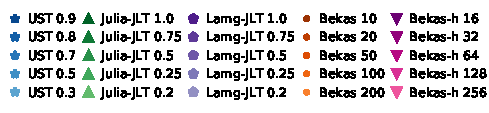
\includegraphics{sources/plots/el-clos/legend-quality.pdf}
\end{subfigure}\smallskip

\begin{subfigure}{.3\textwidth}
\centering
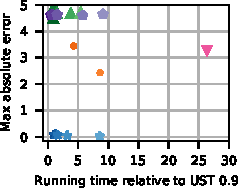
\includegraphics[width=\textwidth]{sources/plots/el-clos/abs-errors.pdf}
\caption{Maximum of the maximum absolute errors.}
\label{fig:el-clos:el-clos-max-abs}
\end{subfigure}\hfill
\begin{subfigure}{.3\textwidth}
\centering
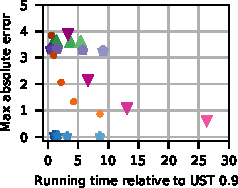
\includegraphics[width=\textwidth]{sources/plots/el-clos/avg-abs-errors.pdf}
\caption{Arithmetic mean of the maximum absolute error.}
\label{fig:el-clos:el-clos-avg-abs}
\end{subfigure}\hfill
\begin{subfigure}{.3\textwidth}
\centering
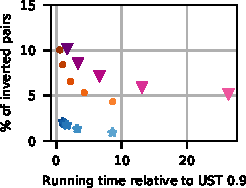
\includegraphics[width=\textwidth]{sources/plots/el-clos/full-ranking.pdf}
\caption{Geometric mean of the percentage of inverted pairs
in the full ranking of $\diag{\Linv}$.}
\label{fig:el-clos:el-clos-full-rank}
\end{subfigure}

\caption{Quality measures over the instances of \Cref{tab:el-clos:insts-ec-med-gt}.
All runs are sequential.}
\label{fig:el-clos:el-clos-quality}
\end{figure}

\Cref{fig:el-clos:el-clos-max-abs} shows that, in terms of maximum absolute error,
every configuration of \ust achieves results with higher quality than the competitors.
Even when setting $\epsilon = \numprint{0.9}$, \ust yields a maximum absolute
error of \ustMaxAbsErr, and it is \ustBekasSpeedup faster than \bekas with 200
random vectors -- which, in turn, achieves a maximum absolute error of \bekasMaxAbsErr.
Furthermore, the running time of \ust does not increase substantially for lower
values of $\epsilon$ and its quality does not deteriorate quickly for higher
values of $\epsilon$.
Regarding the average of the maximum absolute error,
\Cref{fig:el-clos:el-clos-avg-abs} shows that, among the competitors, \bekash
with 256 Hadamard rows achieves the best precision. \ust, however, yields an
average error of \ustAvgAbsErr while also being \ustBekasHSpeedup faster than
\bekash, which yields an average error of \bekasAvgAbsErr. Note also that the
number next to each method in \Cref{fig:el-clos:el-clos-quality} corresponds to
different values of absolute (for \ust) or relative (for \lamgjlt and
\juliajlt) error bounds, and different number of samples (for \bekas and
\bekash). For \bekash, the number of samples needs to be a multiple of four due
to dimension of Hadamard matrices.

In \Cref{fig:el-clos:el-clos-full-rank}, we report the percentage of inverted
pairs in the full ranking of the vertices according to $\diag{\Linvapx}$.
Note that JLT-based approaches are not depicted in this plot because they
yield $>15\%$ of rank inversions. Among the competitors, \bekas achieves the
best time-accuracy trade-off. However, when using 200 random vectors, it yields
\bekasRanking inversions while also being \ustBekasSpeedup slower than \ust
with $\epsilon = 0.9$, which yields \ustRanking inversions only.

For validation purposes, we also measure how well the considered algorithms
compute the \emph{set} (not the ranking) of top-$k$ vertices, \ie those with
highest electrical closeness centrality, with $k\in \set{10, 100}$. For each
algorithm we only consider the parameter settings that yields the highest
accuracy. JLT-based approaches appear to be very accurate for this purpose, as
their top-$k$ sets achieve a Jaccard index of $1.0$. As expected (due to its
absolute error guarantee), \ust performs slightly worse: on average, it obtains
\numprint{0.95} for $k = 10$ and \numprint{0.98} for $k = 100$, which still
shows a high overlap with the ground truth.

\subsection{Memory Consumption}
\begin{figure}[tb]
\centering
\begin{subfigure}{\textwidth}
\centering

\includegraphics{sources/plots/el-clos/legend-memory-consumption.pdf}
\end{subfigure}

\begin{subfigure}{.6\textwidth}
\centering
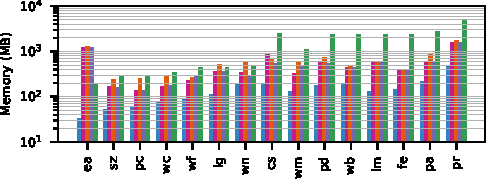
\includegraphics[width=\textwidth]{sources/plots/el-clos/memory-consumption.pdf}
\end{subfigure}
\caption{Difference between the peak resident set size before and after
a sequential run of each algorithm on the instances of
\Cref{tab:el-clos:insts-ec-med-gt,tab:el-clos:insts-ec-med-no-gt}.}
\label{fig:el-clos:memory}
\end{figure}

We measure the peak memory consumption of all the algorithms while running
sequentially on the instances of
\Cref{tab:el-clos:insts-ec-med-gt,tab:el-clos:insts-ec-med-no-gt}.
More precisely, we subtract the peak resident set size before launching
the algorithm from the peak resident size after the algorithm finished.
\Cref{fig:el-clos:memory} shows that \ust requires less memory than the
competitors on all the considered instances. This can be explained by the
fact that, unlike its competitors, our algorithm does not rely on Laplacian
solvers with considerable memory overhead.
For the largest network in particular, the peak memory is \ustMemPR MB for
\ust, and at least \lamgMemPR GB for the competitors.

\subsection{Parallel Scalability}
\label{sec:el-clos:par-scal}
\begin{figure}[tb]
\centering
\begin{subfigure}[t]{.45\textwidth}
\centering
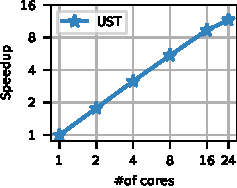
\includegraphics[width=.7\textwidth]{sources/plots/el-clos/ust-sh-mem-scalability.pdf}
\caption{Geometric mean of the speedup of \ust on multiple cores (shared memory)
\wrt a sequential run. Data points are aggregated over the instances of
\Cref{tab:el-clos:insts-ec-med-gt,tab:el-clos:insts-ec-med-no-gt}.}
\label{fig:el-clos:el-clos-sh-mem-scal}
\end{subfigure}\hfill
\begin{subfigure}[t]{.45\textwidth}
\centering
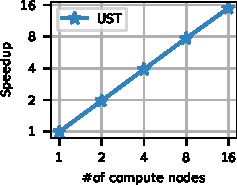
\includegraphics[width=.7\textwidth]{sources/plots/el-clos/ust-distr-mem-scalability.pdf}
\caption{Geometric mean of the speedup of \ust on multiple compute nodes
\wrt \ust on a single compute node ($1\times 24$ cores). Data points
are aggregated over the instances of \Crefrange{tab:el-clos:insts-ec-med-gt}{tab:el-clos:insts-ec-large}.}
\label{fig:el-clos:el-clos-distr-mem-scal}
\end{subfigure}
\caption{Parallel scalability of \ust (with $\epsilon = \numprint{0.3}$) with shared
and with distributed memory.}
\end{figure}

The log-log plot in \Cref{fig:el-clos:el-clos-sh-mem-scal} shows that, on shared memory,
\ust achieves a moderate parallel scalability \wrt the number of cores; on 24 cores in
particular, it is \shmemspeedup faster than on a single core.
Even though the number of USTs to be sampled can be evenly divided among the available
cores, we do not see a nearly-linear scalability: on multiple cores the memory performance
of our NUMA system becomes a bottleneck. Therefore, the time to sample a UST increases
and using more cores yields diminishing returns.
Limited memory bandwidth is a known issue affecting algorithms based on graph traversals
in general~\cite{DBLP:conf/icpp/BaderCF05,DBLP:journals/ppl/LumsdaineGHB07}.

Finally, we compare the parallel performance of \ust indirectly with the
parallel performance of our competitors. Specifically, assuming a perfect
parallel scalability for our competitors \bekas and \bekash on 24 cores, \ust
would yield results \numprint{4.1} and \numprint{12.6} times faster,
respectively, even with this strong assumption for the competition's benefit.

\ust scales better in a distributed setting. In this case, the scalability is affected
mainly by its non-parallel parts and by synchronization latencies.
The log-log plot in \Cref{fig:el-clos:el-clos-distr-mem-scal} shows that, on up to 4
compute nodes, the scalability is almost linear, while on 16 compute nodes \ust
achieves a \distrspeedup speedup \wrt a single compute node.

\begin{figure}[tb]
\centering
\begin{subfigure}[c]{.3\textwidth}
\centering
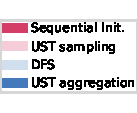
\includegraphics[width=.5\textwidth]{sources/plots/el-clos/legend-time-breakdown.pdf}
\end{subfigure}\hfill
\begin{subfigure}[c]{.6\textwidth}
\centering
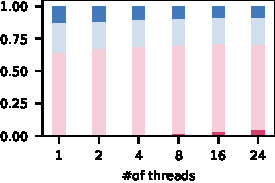
\includegraphics[width=.7\textwidth]{sources/plots/el-clos/time-breakdown.pdf}
\end{subfigure}
\caption{Breakdown of the running times of \ust with $\epsilon = \numprint{0.3}$
\wrt \#of cores on $1\times 24$ cores. Data is aggregated with the geometric
mean over the instances of \Cref{tab:el-clos:insts-ec-med-gt,tab:el-clos:insts-ec-med-no-gt}.}
\label{fig:el-clos:time-breakdown}
\end{figure}

\Cref{fig:el-clos:time-breakdown} shows the fraction of time \ust spends on
different tasks depending on the number of cores. We aggregated over
\enquote{Sequential Init.} the time spent on memory allocation, pivot
selection, solving the linear system, the computation of the biconnected
components, and on computing the BFS tree $B_u$. In all configurations, \ust
spends the majority of the time in sampling, computing the DFS data structures,
and aggregating USTs. The total time spent on aggregation corresponds to
\enquote{UST aggregation} and \enquote{DFS} in
\Cref{fig:el-clos:time-breakdown}, indicating that computing the DFS data
structures is the most expensive part of the aggregation. Together, sampling
time and aggregation time account for \ustFracOneCore and \ustFracAllCores of
the total running time on 1 core and 24 cores, respectively. On average,
sampling takes \avgSampling of this time, while total aggregation takes
\avgAggregate. Since sampling a UST is on average \aggOverSampl more expensive
than computing the DFS timestamps and aggregation, faster sampling techniques
would significantly improve the performance of our algorithm.

\subsection{Scalability to Large Networks}
\begin{figure}[tb]
\centering
\begin{subfigure}[t]{.45\textwidth}
\centering
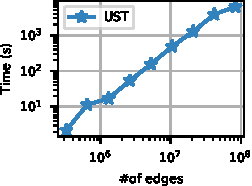
\includegraphics[width=.7\textwidth]{sources/plots/el-clos/hyp-scalability.pdf}
\caption{Running time of \ust \wrt \#of edges.}
\label{fig:el-clos:hyp-running-time}
\end{subfigure}\hfill
\begin{subfigure}[t]{.45\textwidth}
\centering
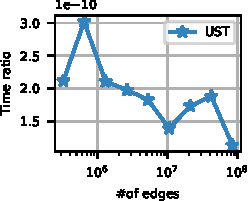
\includegraphics[width=.7\textwidth]{sources/plots/el-clos/hyp-theoretical-scalability.pdf}
\caption{Ratio between the running time of \ust and its theoretical running
time (see \Cref{theo:el-clos:diag-apx-algo}.}
\label{fig:el-clos:hyp-theo-running-time}
\end{subfigure}
\caption{Scalability of \ust on random hyperbolic graphs ($\epsilon = \numprint{0.3}$,
$1\times 24$ cores).}
\end{figure}

\begin{figure}[tb]
\centering
\begin{subfigure}[t]{.45\textwidth}
\centering
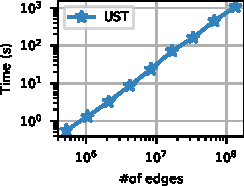
\includegraphics[width=.7\textwidth]{sources/plots/el-clos/rmat-scalability.pdf}
\caption{Running time of \ust \wrt \#of edges.}
\label{fig:el-clos:rmat-running-time}
\end{subfigure}\hfill
\begin{subfigure}[t]{.45\textwidth}
\centering
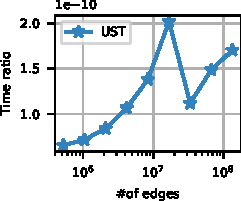
\includegraphics[width=.7\textwidth]{sources/plots/el-clos/rmat-theoretical-scalability.pdf}
\caption{Ratio between the running time of \ust and its theoretical running
time (see \Cref{theo:el-clos:diag-apx-algo}.}
\label{fig:el-clos:rmat-theo-running-time}
\end{subfigure}
\caption{Scalability of \ust on R-MAT graphs ($\epsilon = \numprint{0.3}$,
$1\times 24$ cores).}
\label{fig:el-clos:rmat-scalability}
\end{figure}

\paragraph{Results on Synthetic Networks}
The log-log plot in \Cref{fig:el-clos:hyp-running-time} show the average running time
of \ust $1\times24$ cores on random hyperbolic
networks~\cite{DBLP:conf/hpec/LoozOLM16}.\footnote{The random hyperbolic generator generates
networks with a heavy-tailed degree distribution. We set the average degree to 20 and the
exponent of the power-law distribution to 3.}
For each network size, we take the arithmetic mean of the running times
measured on five different randomly generated networks.
Our algorithm requires \maxTimeHyp minutes for the largest inputs
-- with up to \maxEdgesHyp million edges.
Interestingly, \Cref{fig:el-clos:hyp-theo-running-time} shows that the algorithm
scales slightly better than our theoretical bound predicts.
In \Cref{fig:el-clos:rmat-scalability} we present additional results on R-MAT
graphs~\cite{DBLP:conf/sdm/ChakrabartiZF04}. For this experiment, we use the
Graph 500~\cite{murphy2010introducing} parameter setting -- \ie \graphfh.
On these instances, the algorithm requires only \maxTimeRmat minutes on inputs
with up to \maxEdgesRmat million edges.
In particular, since these graphs have a nearly-constant diameter,
our algorithm is faster than on random hyperbolic graphs.
Qualitatively, it exhibits a similar scalability. The comparison to the theoretical
bound is, however, less conclusive.

\paragraph{Results on Large Real-World Networks}
\begin{table}[tb]
\centering
\small
\captionabove{Running time (s) of \ust on large real-world networks ($16\times 24$ cores).}
\label{tab:el-clos:el-clos-time-cluster}
\begin{tabular}{lrrrr}
\toprule
\multirow{2}{*}{Network} & \multirow{2}{*}{$n$} & \multirow{2}{*}{$m$} & Time (s)  & Time (s) \\
& & & $\epsilon = 0.3$ & $\epsilon = 0.9$ \\
\midrule
petster-carnivore & \numprint{601213} & \numprint{15661775} & \numprint{16.8} & \numprint{4.8}\\
soc-pokec-relationships & \numprint{1632803} & \numprint{22301964} & \numprint{55.5} & \numprint{9.5}\\
soc-LiveJournal1 & \numprint{4843953} & \numprint{42845684} & \numprint{277.0} & \numprint{75.5}\\
livejournal-links & \numprint{5189808} & \numprint{48687945} & \numprint{458.4} & \numprint{80.6}\\
orkut-links & \numprint{3072441} & \numprint{117184899} & \numprint{71.8} & \numprint{19.9}\\
wikipedia\_link\_en & \numprint{13591759} & \numprint{334590793} & \numprint{429.9} & \numprint{88.3}\\
\bottomrule
\end{tabular}
% Generated on: 20/04/2020 22:31:22

\end{table}

In \Cref{tab:el-clos:el-clos-time-cluster} we report the performance of \ust in
a distributed setting ($16\times 24$ cores) on large \emph{real-world} networks.
With $\epsilon = \numprint{0.3}$ and $\epsilon = \numprint{0.9}$, \ust always runs
in less than 8 minutes and $\numprint{1.5}$ minutes, respectively.

\subsection{Additional Experimental Results}
\label{sec:el-clos:rel-err-results}
\paragraph{Relative Error Quality Measures}
Because our algorithm computes an absolute $\pm\epsilon$-approximation of
$\diag{\Linv}$ with high probability, it is expected to yield better
results in terms of maximum absolute error and ranking than numerical approaches
with a relative error guarantee. Indeed, as we show in the following,
the quality assessment changes if we consider quality measures on a relative
error such as:

\begin{align*}
\lonerel &:= \frac{\onenorm{\diag{\Linv} - \diag{\Linvapx}}}{\onenorm{\diag{\Linv}}},\\
\ltworel &:= \frac{\twonorm{\diag{\Linv} - \diag{\Linvapx}}}{\twonorm{\diag{\Linv}}},\\
\erel &:= \text{gmean}_v\frac{\left|\Linv[v, v] - \Linvapx[v, v]\right|}{\Linv[v, v]}.
\end{align*}

\paragraph{Quality in terms of Relative Error}
\begin{figure}[tb]
\centering
\begin{subfigure}{\textwidth}
\centering
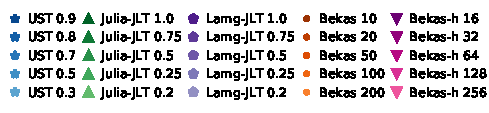
\includegraphics{sources/plots/el-clos/legend-quality.pdf}
\end{subfigure}\smallskip

\begin{subfigure}{.3\textwidth}
\centering
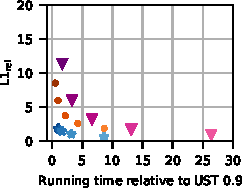
\includegraphics[width=\textwidth]{sources/plots/el-clos/l1-norm.pdf}
\end{subfigure}\hfill
\begin{subfigure}{.3\textwidth}
\centering
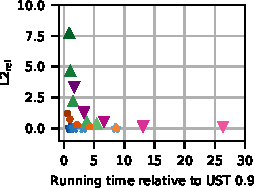
\includegraphics[width=\textwidth]{sources/plots/el-clos/l2-norm.pdf}
\end{subfigure}\hfill
\begin{subfigure}{.3\textwidth}
\centering
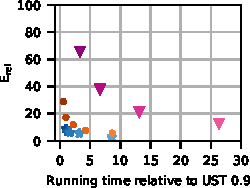
\includegraphics[width=\textwidth]{sources/plots/el-clos/relative-error.pdf}
\end{subfigure}
\caption{$\lonerel$, $\ltworel$, and $\erel$ \wrt the running time of our algorithm
with $\epsilon = \numprint{0.9}$. All data points are aggregated using the geometric
mean over the instances of \Cref{tab:el-clos:insts-ec-med-gt}.}
\label{fig:el-clos:el-clos-quality-rel}
\end{figure}

\Cref{fig:el-clos:el-clos-quality-rel} shows that, when assessing the error in
terms of $\lonerel$, $\ltworel$, or $\erel$, for the same running time, \ust
yields results that are still better in terms of quality than the competitors',
but not by such a wide margin. This can be explained by the fact that the numerical
solvers used by our competitors often employ measures analogous to $\lonerel$
and $\ltworel$ in their stopping conditions.

\section{Experiments -- Forest Closeness}
\label{sec:el-clos:exp-forest}

We now study the empirical performance of our algorithm for forest closeness
(\Cref{sec:el-clos:forest-clos-extension}) on real-world graphs.

\paragraph{Settings} Unless stated otherwise, all algorithms are implemented
in C++, using the NetworKit~\cite{DBLP:journals/netsci/StaudtSM16} graph APIs.
All experiments are conducted on Linux machines equipped with an \CPU
and \RAM each. Unless stated otherwise, all experiments run on a single core.
We manage our experiments with the SimexPal
software~\cite{DBLP:journals/algorithms/AngrimanGLMNPT19} to ensure
reproducibility. For evaluation, we use a large collection of undirected
graphs of different sizes, coming from a diverse set of domains. All graphs
have been downloaded from the public repositories KONECT~\cite{kunegis2013konect},
OpenStreetMap~\cite{OpenStreetMap}, and
NetworkRepository~\cite{DBLP:conf/aaai/RossiA15}.
We denote our proposed algorithm for forest closeness by \ust and,
as done in~\cite{DBLP:conf/icdm/JinBZ19}, we set $\alpha = 1$.

\paragraph{Competitors} For the forest closeness of individual
vertices, the main competitor is the JLT-based algorithm by
Jin \etal~\cite{DBLP:conf/icdm/JinBZ19}, which uses the Laplacian
solver from Ref.~\cite{DBLP:conf/focs/KyngS16}.
We compare against two implementations of this algorithm: one provided
by the authors written in Julia v1.0.2 and our own implementation
based on Eigen's~\cite{eigenweb} CG algorithm. We denote them by
\jltjulia and \jltcpp, respectively. Like in Ref.~\cite{DBLP:conf/icdm/JinBZ19},
we compute the number of linear systems for \jltjulia and \jltcpp
as $\ceil{\frac{\log n}{\epsilon^2}}$ -- which gives an
$(\epsilon\cdot c)$-approximation for a fixed constant $c > 1$.

\subsection{Performance of \ust}
We measure the performance of \ust compared to the state of the art.
Each method is executed with multiple settings of its respective quality
parameter.

\paragraph{Accuracy and Running Time}
\begin{table}[tb]
\setlength{\tabcolsep}{2pt}
\centering
\footnotesize
\caption{Running time and KT ranking scores of \ust
and JLT-based algorithms. In the JLT column we report,
for each instance, the competitor with highest KT score.
For equal KT scores -- up to the second decimal place --
we choose the fastest competitor.}
\label{tab:el-clos:forest-corr}
\begin{subtable}[t]{.5\textwidth}
\centering
\caption{Complex networks}
\label{tab:el-clos:forest-corr-cplx}
\begin{tabular}{lrrrrrrr}
\toprule
\multirow{2}{*}{Graph} & \multirow{2}{*}{$n$} & \multirow{2}{*}{$m$} & \multicolumn{2}{c}{Time (s)} & \multicolumn{2}{c}{KT}\\
& & & UST & JLT & UST & JLT\\
\midrule
loc-brightkite\_edges & 58K & 214K& \textbf{\numprint{46.4}}& \numprint{186.4}& \textbf{\numprint{0.98}}& \numprint{0.95}\\
douban & 154K & 327K& \textbf{\numprint{80.8}}& \numprint{370.9}& \textbf{\numprint{0.71}}& \numprint{0.61}\\
soc-Epinions1 & 75K & 405K& \textbf{\numprint{55.5}}& \numprint{339.6}& \textbf{\numprint{0.95}}& \numprint{0.90}\\
slashdot-zoo & 79K & 467K& \textbf{\numprint{59.9}}& \numprint{412.3}& \textbf{\numprint{0.95}}& \numprint{0.92}\\
petster-cat-household & 105K & 494K& \textbf{\numprint{61.8}}& \numprint{372.1}& \textbf{\numprint{0.98}}& \numprint{0.92}\\
wikipedia\_link\_fy & 65K & 921K& \textbf{\numprint{58.2}}& \numprint{602.9}& \textbf{\numprint{0.98}}& \numprint{0.96}\\
loc-gowalla\_edges & 196K & 950K& \textbf{\numprint{230.9}}& \numprint{1215.5}& \textbf{\numprint{0.99}}& \numprint{0.97}\\
wikipedia\_link\_an & 56K & 1.1M& \textbf{\numprint{50.7}}& \numprint{562.6}& \textbf{\numprint{0.96}}& \numprint{0.93}\\
wikipedia\_link\_ga & 55K & 1.2M& \textbf{\numprint{44.8}}& \numprint{578.6}& \textbf{\numprint{0.98}}& \numprint{0.97}\\
petster-dog-household & 260K & 2.1M& \textbf{\numprint{359.6}}& \numprint{2472.1}& \textbf{\numprint{0.98}}& \numprint{0.96}\\
livemocha & 104K & 2.2M& \textbf{\numprint{107.4}}& \numprint{1429.3}& \textbf{\numprint{0.98}}& \numprint{0.97}\\
\bottomrule
\end{tabular}

\end{subtable}\hfill
\begin{subtable}[t]{.5\textwidth}
\centering
\caption{Road networks}
\label{tab:el-clos:forest-corr-road}
\begin{tabular}{lrrrrrrr}
\toprule
\multirow{2}{*}{Graph} & \multirow{2}{*}{$n$} & \multirow{2}{*}{$m$} & \multicolumn{2}{c}{Time (s)} & \multicolumn{2}{c}{KT}\\
& & & UST & JLT & UST & JLT\\
\midrule
mauritania & 102K & 150K& \textbf{\numprint{98.1}}& \numprint{217.6}& \textbf{\numprint{0.88}}& \numprint{0.77}\\
turkmenistan & 125K & 165K& \textbf{\numprint{118.5}}& \numprint{273.6}& \textbf{\numprint{0.92}}& \numprint{0.85}\\
cyprus & 151K & 189K& \textbf{\numprint{149.4}}& \numprint{315.8}& \textbf{\numprint{0.89}}& \numprint{0.80}\\
canary-islands & 169K & 208K& \textbf{\numprint{185.5}}& \numprint{382.0}& \textbf{\numprint{0.92}}& \numprint{0.84}\\
albania & 196K & 223K& \textbf{\numprint{192.6}}& \numprint{430.2}& \textbf{\numprint{0.90}}& \numprint{0.82}\\
benin & 177K & 234K& \textbf{\numprint{188.1}}& \numprint{406.8}& \textbf{\numprint{0.92}}& \numprint{0.83}\\
georgia & 262K & 319K& \textbf{\numprint{322.1}}& \numprint{605.3}& \textbf{\numprint{0.91}}& \numprint{0.83}\\
latvia & 275K & 323K& \textbf{\numprint{355.2}}& \numprint{665.4}& \textbf{\numprint{0.91}}& \numprint{0.83}\\
somalia & 291K & 409K& \textbf{\numprint{420.1}}& \numprint{747.5}& \textbf{\numprint{0.92}}& \numprint{0.84}\\
ethiopia & 443K & 607K& \textbf{\numprint{825.9}}& \numprint{1209.7}& \textbf{\numprint{0.91}}& \numprint{0.83}\\
tunisia & 568K & 766K& \textbf{\numprint{1200.1}}& \numprint{1629.0}& \textbf{\numprint{0.89}}& \numprint{0.79}\\
\bottomrule
\end{tabular}

\end{subtable}
\end{table}

We report the maximum absolute error of the estimated diagonal values
(\ie $\max_v|\Fmat[v, v] - \Fmatapx[v, v]|$) over all vertices and instances
from \Cref{tab:el-clos:forest-corr}.\footnote{Note that, as for electrical
closeness, the top vertices in the forest closeness ranking are the ones
with the \emph{lowest} $\Fmat[v,v]$ (see \Cref{eq:el-clos:forest-farness});
hence, we also evaluate the ranking accuracy in a following experiment.}
%
As ground truth, we take $\Fmat[v, v]$ values that are computed using
Eigen's~\cite{eigenweb} CG solver with a tolerance of $10^{-9}$;
exact inversion of $(\Lapl + \Ident)$ would be infeasible for many
of the input graphs. A preliminary comparison against the values
if $\Fmat[v, v]$ computed with the NumPy \texttt{pinv} function
demonstrated the CG provides a sufficiently accurate ground truth.

\begin{figure}[tb]
\centering
\begin{subfigure}[t]{\textwidth}
\centering
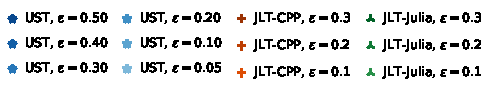
\includegraphics{sources/plots/el-clos/forest-quality-legend.pdf}
\end{subfigure}\smallskip

\begin{subfigure}[t]{.45\textwidth}
\centering
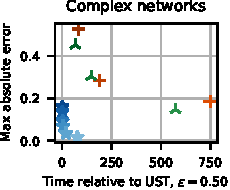
\includegraphics[width=.7\textwidth]{sources/plots/el-clos/forest-max-abs-err-cplx.pdf}
\end{subfigure}\hfill
\begin{subfigure}[t]{.45\textwidth}
\centering
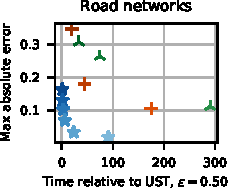
\includegraphics[width=.7\textwidth]{sources/plots/el-clos/forest-max-abs-err-road.pdf}
\end{subfigure}
\caption{$\max_v\left|\Fmat[v, v] - \Fmatapx[v, v]\right|$ over the instances
of \Cref{tab:el-clos:forest-corr}.}
\label{fig:el-clos:forest-quality}
\end{figure}

\Cref{fig:el-clos:forest-quality} shows that \ust achieves the best
results in terms of quality and running time for both complex and road
networks. More precisely, for complex networks and $\epsilon = 0.4$, \ust
yields a maximum absolute error of $\ustMaxAbsFour$, which is less than the
most accurate result of both competitors ($\jltJuliaMaxAbsOne$ achieved by
\jltjulia with $\epsilon = 0.1$), while being $\ustJuliaFourOneSpeedup$ faster.
Also, the running time of \ust does not increase substantially for
lower values of $\epsilon$, and its quality does not deteriorate quickly for
higher values of $\epsilon$. A similar pattern is observed for road networks as
well. Detailed running time values are reported in \Cref{tab:el-clos:forest-time},
\Cref{apx:el-clos:forest-time}.

\paragraph{Vertex Ranking} Moreover, we measure the accuracy in terms of
vertex rankings, which is often more relevant than individual
scores~\cite{DBLP:conf/faw/OkamotoCL08,newman2018networks}.
In \Cref{tab:el-clos:forest-corr}, we report the Kendall's rank correlation
coefficient (KT) of the vertex ranking \wrt the ground truth along with
running times for complex networks (\Cref{tab:el-clos:forest-corr-cplx})
and for road networks (\Cref{tab:el-clos:forest-corr-road}).
%
For each instance, we pick the best run, \ie the \enquote{UST} and
\enquote{JLT} columns display the run with highest respective KT value.
If the values are the same up to the second decimal place, we pick the
fastest one. \ust has consistently the best vertex ranking scores;
at the same time, it is faster than the competitors. In particular,
\ust is on average $\ustJLTSpeedupCplx$ faster than the JLT-based approaches
on complex networks and $\ustJLTSpeedupRoad$ faster on road networks.

\paragraph{Parallel Scalability}
\begin{figure}[tb]
\centering
\begin{subfigure}[t]{.45\textwidth}
\centering
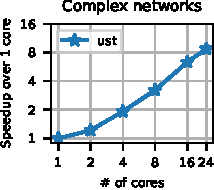
\includegraphics[width=.7\textwidth]{sources/plots/el-clos/parallel-scalability-forest-cplx.pdf}
\end{subfigure}\hfill
\begin{subfigure}[t]{.45\textwidth}
\centering
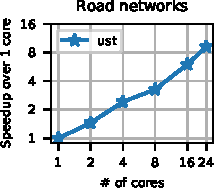
\includegraphics[width=.7\textwidth]{sources/plots/el-clos/parallel-scalability-forest-road.pdf}
\end{subfigure}
\caption{Geometric mean of the speedup of \ust with $\epsilon = \numprint{0.05}$
on multiple cores over a sequential run (shared memory).
Data points are aggregated over the instances of \Cref{tab:el-clos:forest-corr}.}
\label{fig:el-clos:forest-par-scal}
\end{figure}

\begin{figure}[tb]
\centering
\begin{subfigure}[t]{.45\textwidth}
\centering
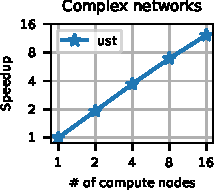
\includegraphics[width=.7\textwidth]{sources/plots/el-clos/distributed-scalability-forest-cplx.pdf}
\end{subfigure}\hfill
\begin{subfigure}[t]{.45\textwidth}
\centering
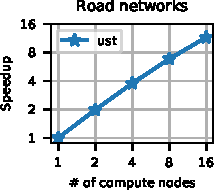
\includegraphics[width=.7\textwidth]{sources/plots/el-clos/distributed-scalability-forest-road.pdf}
\end{subfigure}
\caption{Geometric mean of the speedup of \ust with $\epsilon = \numprint{0.1}$
on multiple compute nodes over a single compute node ($1\times 24$ cores).
Data points are aggregated over the instances of \Cref{tab:el-clos:insts-forest-large}.}
\label{fig:el-clos:forest-distr-scal}
\end{figure}

\begin{table}[tb]
\centering\footnotesize
\setlength{\tabcolsep}{2pt}
\captionabove{Large networks used for scalability experiments
in distributed memory and running time of \ust for forest closeness
on $16\times 24$ cores.}
\label{tab:el-clos:insts-forest-large}
\begin{subtable}[t]{.5\textwidth}
\centering
\caption{Complex networks}
\begin{tabular}{lrrrr}
\toprule
\multirow{2}{*}{Graph} & \multirow{2}{*}{$n$} & \multirow{2}{*}{$m$} & \multicolumn{2}{c}{Time (s)} \\
                       & & & $\epsilon = \numprint{0.1}$ & $\epsilon = \numprint{0.3}$\\
\midrule
soc-LiveJournal1 & \numprint{4846609} & \numprint{42851237} & \numprint{348.9} & \numprint{118.5}\\
wikipedia\_link\_fr & \numprint{3333397} & \numprint{100461905} & \numprint{205.4} & \numprint{90.7}\\
orkut-links & \numprint{3072441} & \numprint{117184899} & \numprint{293.5} & \numprint{92.2}\\
dimacs10-uk-2002 & \numprint{18483186} & \numprint{261787258} & \numprint{1101.3} & \numprint{365.8}\\
wikipedia\_link\_en & \numprint{13593032} & \numprint{334591525} & \numprint{919.3} & \numprint{295.4}\\
\bottomrule
\end{tabular}

\end{subtable}\hfill
\begin{subtable}[t]{.5\textwidth}
\centering
\caption{Complex networks}
\begin{tabular}{lrrrr}
\toprule
\multirow{2}{*}{Graph} & \multirow{2}{*}{$n$} & \multirow{2}{*}{$m$} & \multicolumn{2}{c}{Time (s)} \\
 & & & $\varepsilon = 0.1$ & $\varepsilon = 0.3$\\
\midrule
slovakia & \numprint{543733} & \numprint{638114} & \numprint{28.1} & \numprint{9.9}\\
netherlands & \numprint{1437177} & \numprint{1737377} & \numprint{82.9} & \numprint{31.1}\\
greece & \numprint{1466727} & \numprint{1873857} & \numprint{74.5} & \numprint{29.8}\\
spain & \numprint{4557386} & \numprint{5905365} & \numprint{273.0} & \numprint{86.2}\\
great-britain & \numprint{7108301} & \numprint{8358289} & \numprint{419.0} & \numprint{136.6}\\
dach & \numprint{20207259} & \numprint{25398909} & \numprint{1430.1} & \numprint{473.7}\\
africa & \numprint{23975266} & \numprint{31044959} & \numprint{1493.4} & \numprint{499.3}\\
\bottomrule
\end{tabular}

\end{subtable}
\end{table}

As described in \Cref{sec:el-clos:par-impl}, \ust is well-suited for parallel
implementations since each UST can be sampled independently in parallel.
Hence, we provide parallel implementations of \ust based on OpenMP (for
multi-core parallelism) and MPI (to scale to multiple compute nodes)
for forest closeness as well.

In \Cref{fig:el-clos:forest-par-scal}, we report the parallel scalability of
\ust on multiple cores. Unsurprisingly, analogously to the results achieved in
\Cref{sec:el-clos:par-scal}, \ust exhibits a moderate scalability \wrt the
number of cores. In particular, our OpenMP implementation on 24 cores exhibits
a speedup of $\parSpeedupCplx$ on complex networks and $\parSpeedupRoad$ on
road networks. As with electrical closeness, we hypothesize that this is mainly
due to memory latencies: while sampling a UST, our algorithm performs several
random accesses to the graph data structure (\ie an adjacency
array~\cite{DBLP:journals/netsci/StaudtSM16}), which are prone to cache misses.
%
The results for MPI are depicted in \Cref{fig:el-clos:forest-distr-scal}.
In this setting, \ust obtains a speedup of
$\distrSpeedupCplx$ on complex and $\distrSpeedupRoad$ on road networks
on up to 16 compute nodes -- for this experiment we set $\epsilon = \numprint{0.1}$
and we use the instances in \Cref{tab:el-clos:insts-forest-large}.
More sophisticated load balancing techniques are likely to increase the speedup
in the MPI setting, they are left for future work.
Still, the MPI-based algorithm can rank complex networks with up to $334$M
edges in less than $20$ minutes. Road networks with $31$M edges take less than
$25$ minutes.

\section{Conclusions}
%
This chapter addressed the problem of approximating
electrical centrality measures, namely, electrical closeness, normalized
random-walk betweenness, Kirchhoff-related indices, and forest closeness. The
core contribution is a new efficient parallel algorithm for approximating
$\diag{\Linv}$ of Laplacian matrices \Lapl corresponding to small-world
weighted undirected networks, which is enough to compute the aforementioned
measures. Compared to the main competitors, our algorithm is about one order of
magnitude faster, it yields results with superior quality in terms of absolute
error and ranking of $\diag{\Linv}$, and it requires less memory.

Furthermore, we extended our algorithm to forest closeness, which can now be
approximated faster and more accurately than previously possible. Because the
augmented graph has constant diameter, in the forest closeness case we can
target any graph -- not only small-world graphs \change{-- without
degrading the performance of the algorithm}.

The gap between the theoretical bounds and the much better empirical error
yielded by our algorithm in approximating $\diag{\Linv}$ suggests that tighter
bounds on the number of samples are a promising direction for future research.
Another potentially interesting research direction is to devise a new
UST-based adaptive sampling strategy, as it could reduce the number of samples
and thus the running time of our \ust algorithm and it would benefit
from our epoch-based framework for parallel ADS described in
\Cref{ch:betweenness-approx}.
Other conceivable ideas for future work are an improvement of the running time
for high-diameter graphs, both in theory and in practice, and extensions of our
strategies to directed graphs.

\part{Algorithms for Group Centrality Measures}
\label{part:group-centrality}
\chapter*{Introduction}
%
As we saw in \Cref{part:single-vertex-centrality},
finding highly central vertices in a graph is a fundamental
problem in network analysis (see also Ref.~\cite{newman2018networks}).
To this end, several
centrality measures have been introduced over the past decades (see
Ref.~\cite{DBLP:journals/im/BoldiV14} and \Cref{sec:centrality-measures}).
The problem of identifying the top-$k$ most central vertices in
a graph has been widely studied
\cite{DBLP:journals/tkdd/BergaminiBCMM19,
DBLP:conf/faw/OkamotoCL08,DBLP:conf/icde/OlsenLH14,DBLP:conf/www/LeeC14}.
However, many network analysis applications do not require the $k$
most \emph{individually} central vertices, but rather a \emph{group}
of $k$ vertices that is central \emph{as a whole}
\cite{DBLP:journals/toc/KempeKT15,
DBLP:journals/isci/ZhaoWLTG17,DBLP:journals/pe/GkantsidisMS06,DBLP:conf/icde/LiLCCDZ15,
yan2006efficient}.

Everett and Borgatti~\cite{everett1999centrality}
were the first to extend the centrality concept to groups of vertices and
defined group-degree, group-closeness, group-betweenness, and flow betweenness.
Group centrality maximization problems are often \np-hard: group-degree
maximization can be reduced from vertex cover~\cite{DBLP:conf/alenex/AngrimanGBZGM20},
for group-closeness see Ref.~\cite{DBLP:conf/adc/ChenWW16} and for group-harmonic
see Ref.~\cite{DBLP:conf/alenex/AngrimanBDGGM21}.
Consequently, exact methods for these problems such as ILP
solvers~\cite{DBLP:conf/alenex/BergaminiGM18} take too long on graphs with
non-trivial size -- a few thousands of vertices/edges or more.
Thus, group centrality maximization is generally approached via
approximation~\cite{DBLP:conf/kdd/MahmoodyTU16,DBLP:conf/www/0002PSYZ19}
or heuristics~\cite{DBLP:conf/alenex/BergaminiGM18,DBLP:conf/adc/ChenWW16}.
Yet, existing algorithms for group centrality maximization fail to scale to
large real-world networks. In addition, early attempts to attribute a constant-factor
approximation to a popular greedy algorithm for group-closeness maximization
were flawed (see \Cref{sec:group-harm-clos-max:gc-prel-disc}), leaving the open
questions of whether this problem can be approximated and, if so, how well.
Another weakness of existing group centrality measures is that, without proper
adjustments, they are not designed to handle disconnected graphs.

In the following, we address the lack of scalability of group centrality
maximization algorithms from two directions: (i) in the context of
group-closeness centrality, we introduce new fast local search heuristics to
compute highly central groups of vertices in large graphs
(\Cref{ch:group-closeness-local-search}) and (ii) we introduce a novel
group centrality measure called GED-Walk as well as efficient parallel
algorithms compute it and to approximate the group of vertices with highest
GED-Walk centrality (\Cref{ch:ged-walk}).
%
Concerning the group-closeness approximation issue, building on top of the
results presented in Ref.~\cite{DBLP:conf/alenex/AngrimanBDGGM21}, we provide
an efficient implementation of the first approximation algorithm for this
problem (\Cref{ch:group-harm-clos-max}). Finally, we address the lack of
electrical group centrality measures for disconnected graphs by extending
forest closeness to disconnected graphs (\Cref{ch:ged-walk}); as its
single-vertex counterpart, group forest closeness handles disconnected graphs
out of the box.

\paragraph{Contribution and Outline}
In \Cref{ch:group-closeness-local-search}, we introduce new fast local search
heuristics for group-closeness to compute highly central groups of vertices.
Our heuristics start from an initial a group of vertices $S$ and perform
exchanges between vertices within $S$ and the rest of the graph until they
reach a local optim\change{um}. Compared to the state-of-the-art greedy
algorithm~\cite{DBLP:conf/alenex/BergaminiGM18}, experimental results show
that, on unweighted graphs, our strategy is two orders of magnitude faster and
achieves $\numprint{99.4}\%$ of the solution quality; on weighted graphs, it
yields solutions of $\onedigit{\wGSQualInc}\%$ \emph{higher} quality while also
being $\onedigit{\gsPSevenFiveKSpeed}\times$ faster.
Furthermore, our algorithms handle graphs with hundreds of million of edges
in only around ten minutes, while the greedy algorithm requires more than
ten \emph{hours}.

Heuristics, however, do not provide any approximation guarantees, leaving
the question of approximability for group-closeness maximization unsettled.
In \Cref{ch:group-harm-clos-max}, we address this issue.
By exploiting the theoretical results
from Ref.~\cite{DBLP:conf/alenex/AngrimanBDGGM21}, we build the first
approximation algorithm for group-closeness maximization by adapting to
group-closeness the local search algorithm for $k$-Median by Arya
\etal~\cite{DBLP:journals/siamcomp/AryaGKMMP04}. In
addition, we also address \emph{group-harmonic} maximization -- to
the best of our knowledge, we are the first to study this optimization problem.
We implement an efficient greedy algorithm as well as a local search
approximation algorithm to maximize group-harmonic.
In our experimental study we show that, compared to a greedy strategy, our local
search approximation algorithm yields solutions with superior quality at the cost
of additional running time. In particular, local search is one to three orders
of magnitude slower than greedy, which is expected due to the approximation
guarantees. Indeed, local search approximation algorithms often cut greedy's
(empirical) gap to optimality by half or more.

Finally, in \Cref{ch:ged-walk}, we introduce two new group centrality
measures: GED-Walk, a novel group centrality
measure inspired by Katz centrality, and group forest closeness, that is, forest
closeness (see \Cref{ch:electrical-closeness}) extended to sets of vertices.
Similarly to Katz centrality, GED-Walk takes into account walks of any length
and gives to shorter walks greater importance than to longer walks. Since it is
not based on shortest paths, GED-Walk can be optimized significantly faster
(for groups with moderate size) compared to shortest-path based measures such
as group-closeness, group-harmonic or group-betweenness.
%
We describe efficient parallel algorithms to
compute the GED-Walk score of a given group and to efficiently approximate the
group of vertices with highest GED-Walk centrality. Experimental results show
that GED-Walk improves the precision of popular graph mining applications
such as semi-supervised vertex classification and graph
classification~\cite{DBLP:journals/tnn/ChapelleSZ09}. Also, our
algorithm for maximizing GED-Walk (in approximation) is two orders of magnitude
faster than state-of-the-art algorithms for group-betweenness
maximization~\cite{DBLP:conf/kdd/MahmoodyTU16} and, for group sizes up to 100
vertices, one to two orders of magnitude faster than group-harmonic and
group-closeness maximization~\cite{DBLP:conf/alenex/BergaminiGM18}.

Group forest closeness, in turn, is defined as the reciprocal of group
forest farness, \ie the sum of forest distances from a group $S$ to the
other vertices. Maximizing this measure turns out to be \np-hard, so we adapt
the greedy approximate algorithm from Li \etal~\cite{DBLP:conf/www/0002PSYZ19}
for group electrical closeness to group forest closeness.
Semi-supervised vertex classification results on disconnected graphs indicate
that, in comparison to existing measures, group forest closeness improves the
precision to a much greater extent.

%%%%%%%%%%%%%%%%%%%%%%%%%%%%%%%%%%%%%%%%%%%%%%%%%%%%%%%%%%%%%%%%%%%%%%%%
\chapter{Local Search for Group-Closeness Maximization on Big Graphs}
\label{ch:group-closeness-local-search}
% Labels: heuristic, static, distance-based (closeness), sequential
%%%%%%%%%%%%%%%%%%%%%%%%%%%%%%%%%%%%%%%%%%%%%%%%%%%%%%%%%%%%%%%%%%%%%%%%

%% For the examples with tikz %%
\newcommand{\coorda}{2.7, 0}
\newcommand{\nodeida}{s1}

\newcommand{\coordb}{2.5, 1}
\newcommand{\nodeidb}{s2}

\newcommand{\coordc}{2.5, -1}
\newcommand{\nodeidc}{s3}

\newcommand{\coordd}{2, -1.6}
\newcommand{\nodeidd}{s4}

\newcommand{\coorde}{1, 0}
\newcommand{\nodeide}{s5}

\newcommand{\coordf}{.75, .6}
\newcommand{\nodeidf}{s6}
\newcommand{\coordg}{3, -2.2}
\newcommand{\nodeidg}{n1}

\newcommand{\coordh}{3.8, -0.8}
\newcommand{\nodeidh}{n2}

\newcommand{\coordi}{3.7, 0}
\newcommand{\nodeidi}{n3}

\newcommand{\coordj}{3.5, 0.7}
\newcommand{\nodeidj}{n4}

\newcommand{\coordk}{5, -2.1}
\newcommand{\nodeidk}{n5}

\newcommand{\coordl}{5.1, -1.5}
\newcommand{\nodeidl}{n6}

\newcommand{\coordm}{5.9, -0.8}
\newcommand{\nodeidm}{n7}

\newcommand{\coordn}{5.7, 0}
\newcommand{\nodeidn}{n8}

\newcommand{\coordo}{5.5, 1}
\newcommand{\nodeido}{n9}

\newcommand{\coordp}{7.5, -1.2}
\newcommand{\nodeidp}{n10}

\newcommand{\coordq}{7.7, 0}
\newcommand{\nodeidq}{n11}

\newcommand{\coordr}{7, 0.7}
\newcommand{\nodeidr}{n12}

\newcommand{\edgecoords}{
\path (s1) ++(0:\nshift) coordinate (sg1);
\path (s1) ++(-30:\nshift) coordinate (sg11);
\path (s1) ++(90:\nshift) coordinate (sg12);
\path (s1) ++(0:\nshift) coordinate (sg1);
\path (s2) ++(-20:\nshift) coordinate (sg2);
\path (s2) ++(180:\nshift) coordinate (sg2b);
\path (s2) ++(270:\nshift) coordinate (sg2bb);
\path (s3) ++(0:\nshift) coordinate (sg3);
\path (s3) ++(150:\nshift) coordinate (sg3b);
\path (s4) ++(-30:\nshift) coordinate (sg4);
\path (s5) ++(-30:\nshift) coordinate (sg5);
\path (s6) ++(15:\nshift) coordinate (sg6);

\path (n1) ++(150:\nshift) coordinate (ng1);
\path (n2) ++(180:\nshift) coordinate (ng2);
\path (n2) ++(150:\nshift) coordinate (ng21);
\path (n3) ++(180:\nshift) coordinate (ng3);
\path (n4) ++(165:\nshift) coordinate (ng4);
\path (n1) ++(0:\nshift) coordinate (ng1b);
\path (n2) ++(0:\nshift) coordinate (ng2b);
\path (n2) ++(30:\nshift) coordinate (ng2b1);
\path (n2) ++(-30:\nshift) coordinate (ng2b2);
\path (n3) ++(0:\nshift) coordinate (ng3b);
\path (n3) ++(30:\nshift) coordinate (ng3b1);

\path (n5) ++(180:\nshift) coordinate (ng5);
\path (n6) ++(150:\nshift) coordinate (ng6);
\path (n7) ++(180:\nshift) coordinate (ng7);
\path (n8) ++(180:\nshift) coordinate (ng8);
\path (n8) ++(210:\nshift) coordinate (ng81);
\path (n9) ++(210:\nshift) coordinate (ng9);

\path (n7) ++(-10:\nshift) coordinate (ng6b);
\path (n8) ++(0:\nshift) coordinate (ng7b);
\path (n8) ++(30:\nshift) coordinate (ng7b1);
\path (n9) ++(0:\nshift) coordinate (ng8b);

\path (n10) ++(160:\nshift) coordinate (ng10);
\path (n11) ++(180:\nshift) coordinate (ng11);
\path (n12) ++(210:\nshift) coordinate (ng12);
}

\newcommand{\grouplegend}{
\node[align=right] at (-1.25, .25) {$S$};
\draw[groupstyle,black] (-.75, .25) to (-.25, .25);
}

\newcommand{\graphlegend}{
\grouplegend
\node[align=right] at (-1.25, -.25) {\textnormal{DAG}};
\draw[black] (-.75, -.25) to (-.25, -.25);
}

\newcommand{\graphcoords}{
\coordinate[] (g1) at (0, 0);
\coordinate[] (g2) at (2, -2);
\coordinate[] (g3) at (4, -3);
\coordinate[] (g4) at (6, -2);
\coordinate[] (g5) at (8, -1);
\coordinate[] (g6) at (9, 0);
\coordinate[] (g7) at (7, 1);
\coordinate[] (g8) at (3, 1.2);
}

\newcommand{\drawgroupcontour}{
\coordinate[] (s1) at (3, 0);
\coordinate[] (s2) at (2, 0);
\coordinate[] (s4) at (2.5, 1.3);
\draw[dashed, thick] (s2) to[out=-90,in=180] ([yshift=5pt]g2);
\draw[dashed, thick] ([yshift=5pt]g2) to[out=0,in=-90] (s1);
\draw[dashed, thick] (s1) to[out=90,in=0] (s4);
\draw[dashed, thick] (s4) to[out=180,in=90] (s2);
}

\newcommand{\drawswapgroupcontour}{
\coordinate[] (s1) at (4.5, -1);
\coordinate[] (s11) at (3.25, 0);
\coordinate[] (s2) at (2.3, 0);
\coordinate[] (s22) at (3, -1.2);
\coordinate[] (s23) at (1.75, -1.5);
\coordinate[] (s3) at (2.5, 1.3);
\draw[dashed, thick] (s23) to[out=-90,in=180] ([xshift=-5pt,yshift=2pt]g2);
\draw[dashed, thick] ([yshift=2pt]g2) to[out=0,in=-90] (s1);
\draw[dashed, thick] (s1) to[out=90,in=-90] (s11);
\draw[dashed, thick] (s11) to[out=90,in=0] (s3);
\draw[dashed, thick] (s3) to[out=180,in=150] (s2);
\draw[dashed, thick] (s2) to[out=-30,in=60] (s22);
\draw[dashed, thick] (s22) to[out=240,in=90] (s23);
}


\section{Introduction}
\label{sec:lsh-gc-intro}
Closeness centrality is one of the oldest and most widely-used vertex
centrality measures (see Ref.~\cite{bavelas1948mathematical} and
\Cref{ch:dyn-topk}). It is defined as the
reciprocal of the average shortest-path distance from
a vertex to all the others -- see \Cref{eq:def:closeness}.

Group-closeness can be interpreted as a special case (on graphs)
of the well-known $k$-Median problem for facility location.
Example of applications include: (i) retailers that want to advertise
their products via social media; promoters could be selected as the
group of $k$ members with highest centrality in order to maximize the
influence over the other members~\cite{DBLP:journals/isci/ZhuWWZ14};
(ii) in P2P networks, shared resources could be placed on $k$ peers so
that they are easily accessible by others~\cite{DBLP:journals/pe/GkantsidisMS06};
(iii) in citation networks, group centrality measures can be employed as
alternative indicators for the influence of journals or papers within
their research field~\cite{DBLP:journals/jasis/Leydesdorff07a}.

The problem of finding the group of $k$ vertices with highest group-closeness
(group closeness maximization) is shown to be
\np-hard~\cite{DBLP:conf/adc/ChenWW16}. While exact algorithms to find a group
with maximal closeness are known -- \eg algorithms based on Integer Linear
Programming (ILP)~\cite{DBLP:conf/alenex/BergaminiGM18} -- they do not scale to
graphs with more than a few thousand edges. Hence, in practice, groups with
high closeness centrality are computed through
heuristics~\cite{DBLP:conf/adc/ChenWW16,DBLP:conf/alenex/BergaminiGM18}.

\paragraph{Related Work}
%
For group-betweenness maximization, sampling-based algorithms have been
proposed~\cite{DBLP:conf/kdd/MahmoodyTU16,DBLP:conf/kdd/Yoshida14}. An
extensive analysis of algorithms for group-betweenness estimation is provided
by Chehreghani \etal~\cite{DBLP:conf/bigdataconf/ChehreghaniBA18}, who also
introduce a new algorithm based on an alternative definition of distance
between a vertex and a set of vertices.

Concerning group-closeness maximization, in Ref.~\cite{DBLP:conf/www/ZhaoLTG14}
the definition of group-closeness differs from the original one and only serves
as an estimate of the original -- we use the latter, defined in
\Cref{eq:prelim:gclos}, which is widely accepted. Therefore, their \np-hardness
and submodularity proofs do not necessarily carry over to the original
definition. In fact, the standard group-closeness is not submodular (see
\Cref{lemma:prelim:gclos-not-submod}). Hence, submodular optimization results
in~\cite{DBLP:conf/focs/Vondrak09} do not apply to this case directly.
%
Chen \etal~\cite{DBLP:conf/adc/ChenWW16} argued that group-closeness
maximization is \np-hard by relating it to the \np-hard $k$-means problem.
Their proposed greedy algorithm was later improved by Bergamini
\etal~\cite{DBLP:conf/alenex/BergaminiGM18}, who made algorithm more
memory-efficient and exploited the supermodularity of the reciprocal
of group-closeness for search pruning.
%
Exploiting the supermodularity of the reciprocal also works when the distance
function is replaced by the resistance distance (see
\Cref{sec:prelim-resistance-distance}). This leads to the so-called group
\emph{current-flow} closeness, for which Li
\etal~\cite{DBLP:conf/www/0002PSYZ19} proposed approximation algorithms based
on greedy strategies and random projections.

\paragraph{Motivation}
Still, even for group-closeness with the usual graph distance, the greedy
algorithm can be time-consuming on large instances. Indeed, pruning is most
effective when the group is already large. When performing the first addition,
however, the greedy algorithm has to perform one (pruned) SSSP
\emph{for each vertex in the graph} to compute its marginal contribution, and
this phase scales superlinearly in the size of the graph.
As a result, real-world graphs with hundreds of millions of edges still require
several hours to complete.
%
This motivates us to develop new local search heuristics that quickly find
highly central groups of vertices on large-scale real-world
graphs without sacrificing too much solution quality.

\paragraph{Contribution}
%
In this chapter, we develop new heuristic algorithms for group-closeness
maximization. Specifically, we present two
novel local search heuristics that start from an initial group of vertices $S
\subset V$ and perform exchanges of vertices from $S$ and $V \setminus S$ until
a local optima is reached. The first algorithm, \localswaps, requires little
time per iteration but only exchanges vertices locally. The second algorithm,
\growshrink, performs also non-local vertex exchanges, but iterations are more
computationally expensive.

Experiments on unweighted graphs show that \emph{extended} \growshrink, a
variation of \growshrink, computes groups with closeness scores greater than
$\onedigit{\gsPSevenFiveKQualNum}\%$ of the score of a greedy solution while
being $\onedigit{\gsPSevenFiveKSpeed}\times$ faster (results for $k= 10$).
We see \emph{extended} \growshrink as the best trade-off between
speed and solution quality.
%
When quality is not a primary concern, our other algorithms accelerate the
computation by sacrificing solution quality. For example, for groups with size
10 the non-extended variant of \growshrink yields solutions whose quality is
$\numprint{91.1}\%$ compared to the state of the art while being
$\numprint{700.2}\times$ faster.
The speedup varies between $\onedigit{\gsMaxSpeed}\times$
and $\onedigit{\gsMinSpeed}\times$ for groups with sizes 5 and 100,
respectively.
%
On weighted graphs, our algorithms improve both the quality and
the running time performance of the state of the art: for example, for $k = 10$,
they return solutions of $\onedigit{\wGSQualInc}\%$ higher
quality with a $\onedigit{\wGSSpeed}\times$ speedup. Different trade-offs
between quality and running time are possible, we discuss them in
\Cref{sec:lsh-gc-experiments-ls}.

\bibnotes{The contributions presented in this chapter
were published in the Proceedings of the
\emph{IEEE International Conference on Big Data, 2019}.
My contributions involve the development of the initial algorithm that led
to the ones presented in the paper. The development of
the presented algorithms is a collaborative effort with Alexander van der
Grinten. Further, I implemented all the presented algorithms
(acceleration techniques with SIMD vector operations were implemented together
with Alexander van der Grinten) and
carried out the experiments.
The rest is joint work with Alexander van der Grinten and Henning Meyerhenke.
Proofs to which I did not contribute are omitted and can
be found in the original paper~\cite{DBLP:conf/bigdataconf/AngrimanGM19}.}


\section{Preliminaries}
\label{sec:lsh-gc-preliminaries}
%
Let $S \subset V$ be a group of vertices. As reported in
\Cref{sec:group-centrality-measures}, the group-closeness centrality of $S$ is
defined as $\gclos(S) := \frac{n}{\sum_{u \in V \setminus S} d(S, u)}$. In the
literature, a similar objective has been addressed as well, namely, the farness
of a set $S$, defined as $\gfarn (S) := \frac{1}{n}\cdot \sum_{u \in V
\setminus S}d(S, u)$. Note that the farness of a group is defined as the
reciprocal of its closeness.


\paragraph{Problem Addressed}
%
In this chapter, we study the problem of finding groups that maximize
group-closeness and subject to a cardinality constraint, \ie for a given
integer $1 \le k < n$, our objective is to find a group with size $k$ of large
group-closeness. Formally:

\begin{cproblem}{Group-Closeness Maximization}
\begin{tabular}{ll}
\textbf{Input:} & Graph $G = (V, E, w)$, integer $1 \le k < n$.\\
\textbf{Find:} & Set $S^\star \subset V$ with $|S| = k$ s.t. $\gclos(S^\star)$ is maximum.
\end{tabular}
\end{cproblem}

We assume $G$ to be undirected, connected, and with positive edge weights.
We consider the problem of improving the group-closeness of a given
set $S$ of vertices with local search. More precisely, we consider
\emph{exchanges} of vertices from $S$ and $V \setminus S$. Let $u$ be a vertex
in $S$ and $v \in V \setminus S$. To simplify the presentation, we use the
notation $\Suv := (S \setminus \set{u}) \cup \set{v}$ to denote the set
resulting by the exchange of $u$ with $v$. We also use the
notation $\Su := S \setminus \set{u}$ and $\Sv := S \cup \set{v}$ to denote
vertex removals and insertions, respectively.

As our algorithms can only perform vertex exchanges, before they can start
they require the construction of an initial solution $S$. Since a superlinear
initialization step would compromise our algorithms' running times, for all our
local search algorithms we choose the initial set $S$ uniformly at random.
%
For large graphs, this initialization can be expected to cover the graph
reasonably well. Exploratory experiments revealed that our algorithms do not
benefit from other obvious initialization techniques -- such as selecting the
$k$ vertices with highest degree.


\section{Estimating the Quality of Vertex Exchanges}
\label{sec:lsh-gc-quality-vertex-exchanges}
%
The greedy ascent algorithm starts with an empty set $S$ and iteratively adds
vertices $v \in V \setminus S$ to $S$ that maximize
$\gfarn(S) - \gfarn(\Sv)$~\cite{DBLP:conf/alenex/BergaminiGM18}.
Depending on the input graph and the value of $k$, however, the greedy algorithm
might need to evaluate the difference in $\gfarn$ for a substantial number
of vertices, and this is rather expensive for large real-world graphs.

The algorithms we present in this section aim to improve upon the running time
of the greedy algorithm. We achieve this by first considering exchanges with
only \emph{local} vertices, \ie vertices that already \enquote{near} $S$.
Clearly, selecting only local vertices would decrease the quality of a greedy solution --
as the greedy algorithm does not have the ability to correct suboptimal choices.
However, this is not necessarily true for our algorithms based on vertex exchanges.
Then, we generalize this strategy by extending vertex exchanges to non-local vertices,
and allowing exchanges of multiple vertices per time
(\Cref{sec:lsh-gc-variants}).

To make our notion of locality more concrete, let $B_S \subseteq G$ be the DAG
constructed by running a SSSP from the vertices in $S$. Here, all the vertices
in $S$ are considered as sources of the SSSP, \ie they are at distance 0.
Further, define
%
\[
\deltafarnm(v) :=
\gfarn(S) - \gfarn(\Sv) = \sum_{x\in V\setminus S}d(S, x) - d(\Sv, x).
\]

To compute the greedy solution, it seems to be necessary to compute $\deltafarnm$
exactly for a substantial number of vertices. Pruning techniques can avoid some of the
computational costs~\cite{DBLP:conf/alenex/BergaminiGM18}, but many evaluations of
$\deltafarnm$ still have to be performed, which seems to be impractical for
large graphs. However, a lower bound for $\deltafarnm$ can be computed from the
shortest-path DAG $B_S$. To this end, let $D_v$ be the set of vertices
reachable from $v$ in $B_S$.

\begin{lemma}
\label{lemma:delta-group-farness}
\change{\cite{DBLP:conf/bigdataconf/AngrimanGM19}} It holds that:
%
\[\deltafarnm(v) \ge |D_v| \cdot d(S, v)\]

In the unweighted case, equality holds if $v$ is a neighbor of $S$.
\end{lemma}

\begin{figure}[t]
\centering
\begin{tikzpicture}

\graphcoords
\graphlegend
\drawgroupcontour

\simplenode{\nodeida}{\coorda}
\simplenode{\nodeidb}{\coordb}
\simplenode{\nodeidc}{\coordc}
\simplenode{\nodeidd}{\coordd}
\simplenode{\nodeide}{\coorde}
\simplenode{\nodeidf}{\coordf}

\simplenode{\nodeidg}{\coordg}
\simplenode{\nodeidh}{\coordh}
\colortextnode{\nodeidh}{\nodeidh}{$v$}
\simplenode{\nodeidi}{\coordi}
\simplenode{\nodeidj}{\coordj}

\simplenode{\nodeidk}{\coordk}
\colornode{\nodeidl}{\coordl}
\colornode{\nodeidm}{\coordm}
\colornode{\nodeidn}{\coordn}
\simplenode{\nodeido}{\coordo}

\colornode{\nodeidp}{\coordp}
\colornode{\nodeidq}{\coordq}
\colornode{\nodeidr}{\coordr}

\edgecoords

\draw[->] (sg1) -- (ng3);
\draw[->] (sg11) -- (ng21);
\draw[->] (sg2) -- (ng4);
\draw[->] (sg3) -- (ng2);
\draw[->] (sg4) -- (ng1);
\draw[<-] (sg5) -- (sg3b);
\draw[<-] (sg6) -- (sg2b);

\draw[->] (ng1b) -- (ng5);
\draw[->,\darkorange,thick] (ng2b2) -- (ng6);
\draw[->,\darkorange,thick] (ng2b) -- (ng7);
\draw[->,\darkorange,thick] (ng2b1) -- (ng81);
\draw[->] (ng3b) -- (ng8);
\draw[->] (ng3b1) -- (ng9);

\draw[->,\darkorange,thick] (ng6b) -- (ng10);
\draw[->,\darkorange,thick] (ng7b) -- (ng11);
\draw[->,\darkorange,thick] (ng7b1) -- (ng12);

\node[] at (10, -1) {\textnormal{Here:} \emph{$|D_v| = 7$}};
\end{tikzpicture}

\caption{Example of shortest-path DAG $B_S$; orange vertices are
in $D_v$.}
\label{fig:lsh-gc:dag}
\end{figure}

An illustration of \Cref{lemma:delta-group-farness} is shown
in \Cref{fig:lsh-gc:dag}.
This bound will be used in the two algorithms presented in
\Cref{sec:lsh-gc-local-swaps,sec:lsh-gc-grow-shrink}.
Instead of picking vertices that maximize $\deltafarnm$, those algorithms pick
vertices that maximize the right-hand side of \Cref{lemma:delta-group-farness}, \ie
$D_v \cdot d(S, v)$.
The bound is local in the sense that it is more accurate for vertices near $S$:
in particular, let $N(S)$ be set of vertices that have a neighbor in $S$; the
reachability sets of vertices in $N(S) \setminus S$
are larger in $G$ than those in $B_S$, as $B_S$ does not contain back edges.
Unfortunately, computing the cardinality of $D_v$ for all
$v$ seems to be prohibitively expensive: indeed, the fastest know algorithm
to compute the size of the transitive closure of a DAG relies on iterated (Boolean)
matrix multiplication -- hence, the best known exact algorithm has a complexity
of $\Oh(n^{\numprint{2.373}})$~\cite{DBLP:conf/soda/AlmanW21}.
However, we can use Cohen's randomized algorithm~\cite{DBLP:journals/jcss/Cohen97}
to approximate the sizes of $D_v$ for all $v$ \emph{at the same time}.
In multiple iterations, this algorithm samples a random number for each vertex
in $G$, accumulates in each vertex $v$ the minimal random number of any vertex
reachable from $v$, and estimates $|D_v|$ based on this information.

We remark that Cohen's algorithm yields an approximation, not a lower bound for
the right-hand side of \Cref{lemma:delta-group-farness}, therefore in our
algorithms the inequality of the Lemma can be violated; in particular, it can
happen that our algorithms pick a vertex $v$ such that $\deltafarnm(v) < 0$.
In this case, instead of decreasing the closeness centrality of the current group,
our algorithms terminate. Nevertheless, our experiments demonstrate that, on real-world
instances, a coarse approximation of the reachability set size is enough for
\Cref{lemma:delta-group-farness} to identify useful candidates for vertex exchanges
(see \Cref{sec:lsh-gc-experiments-ls}).


\section{The \localswaps Algorithm}
\label{sec:lsh-gc-local-swaps}
%

Let us first focus on unweighted graphs. A straightforward idea to construct a
fast local search algorithm is to allow \emph{swaps} betweenness vertices in $S$
and their neighbors in $V \setminus S$. This procedure can be repeated until no
swap can decrease $\gfarn(S)$. Let $u$ be a vertex in the group and let $v \in
N(S)\setminus S$ be one of its neighbors outside the group. To determine whether
swapping $u$ and $v$ (\ie replacing $S$ by $\Suv$) is beneficial, we have to
check whether $\gfarn(S) - \gfarn(\Suv) > 0$, \ie whether the farness decreases
after the swap. The challenges here are (i) to find a pair $u, v$ that satisfies such
inequality without checking all pairs $u, v$ exhaustively and (ii) to compute
the difference $\gfarn(S) - \gfarn(\Suv)$ quickly.
%
Note that a crucial property that allows us to construct an efficient algorithm
is that, after a swap, the distance from $S$ to any other vertex can only
change by $\pm1$. Hence, to compute $\gfarn(S) - \gfarn(\Suv)$, it suffices to
count the number of vertices where the distance changes by $-1$ and the number
of vertices where it changes by $+1$.
To this end, our algorithm requires a few auxiliary data structures; in
particular, we store the following:
\begin{itemize}
    \item the distance $d(S, x)$ from $S$ to all vertices $x \in V \setminus S$;
    \item a set $\lambda_x := \set{s \in S : d(S, x) = d(s, x)}$ for each
        vertex $x\in V\setminus S$ that contains all vertices in $S$ that
        realize the shortest distance from $S$ to $x$;
    \item the value $|\Lambda_s|$ for each $s\in S$, where
        $\Lambda_s := \set{x \in V\setminus S : \lambda_x = \set{s}}$ is the
        set of vertices for which the shortest distance is realized
        \emph{exclusively} by $s$.
\end{itemize}

Note that the sets $\lambda_x$ consume $\Oh(kn)$ memory in total. However,
since $k \ll n$, we can afford this even for large real-world
graphs.\footnote{In our implementation, we store each $\lambda_x$ in only
$k$ bits.}

All of those auxiliary data structures can be maintained dynamically during
the entire algorithm with little additional overhead. More precisely,
after a $u$-$v$ swap is done, $v$ is added to all $\lambda_x$ satisfying
$d(v, x) = d(S, x)$; for $x \in V \setminus S$ such that $d(v, x) < d(S, x)$,
the set $\lambda_x$ is replaced by \set{v}. Vertex $u$ can be removed from all
$\lambda_x$ by a linear-time scan through all $x \in V \setminus S$.

\begin{algorithm}[tb]
\caption{Overview of the \localswaps Algorithm}
\label{algo:local-swaps}
\begin{algorithmic}[1]
\Repeat
\State approximate $D_v$ for all $v \in V \setminus S$ with~\cite{DBLP:journals/jcss/Cohen97}
\State$\left< u, v \right> \gets \argmax_{u, \in S,\ v\in N(u) \setminus S} |D_v| - |\Lambda_u|$
\label{line:ghc-ls-good-swap}
\State$S \gets \Suv$
\State run pruned BFS from $v$\Comment{to recompute $\gfarn(S)$}
\label{line:ghc-ls-pruned-bfs}
\Until{previous iteration did not decrease $\gfarn(S)$}
\end{algorithmic}
\end{algorithm}


\Cref{algo:local-swaps} states a high-level overview of our \localswaps
algorithm. In the following, we discuss how we pick a \enquote{good} swap
(\Cref{line:ghc-ls-good-swap} of the pseudocode) and how to update the data
structures after a swap (\Cref{line:ghc-ls-pruned-bfs}).
The running time of the algorithm is dominated by the initialization of
$\lambda_x$. Thus, it runs in $\Oh(kn + m)$ time per swap.


\subsection{Choosing a Good Swap}
\label{sec:local-swaps-choosing}
%
Because it would be too expensive to compute the exact difference in $\gfarn$
for each possible swap, we find the pair of vertices $\left<u, v\right>$ such
that:
%
\begin{align*}
\left<u, v\right> &= \argmax_{\substack{u \in S,\\v\in N(S) \setminus S}}
|D_v|\cdot d(S, v) - |\Lambda_u|\\
                  &= \argmax_{\substack{u \in S,\\v\in N(S) \setminus S}}
                  |D_v| - |\Lambda_u|.
\end{align*}

Note that this value is a lower bound for the decrease of $\gfarn(S)$ after
swapping $u$ and $v$: In particular, \Cref{lemma:delta-group-farness} implies
that $|D_v|$ is a lower bound for the decrease in farness when adding $v$ to
$S$. Additionally, $|\Lambda_u|$ is an upper bound for the increase in farness
when removing $u$ from $S$ -- and thus also for the increase in farness when
removing $u$ from $\Sv$.\footnote{Note, however, that this bound is trivial if
$|D_v| - |\Lambda_u| \le 0$.} Hence,
we can expect this strategy to yield pairs of vertices that lead to a decrease
of $\gfarn$. In practice, to maximize $|D_v| - |\Lambda_u|$, for each $v \in V
\setminus S$ we first compute the neighbor $u \in N(v) \cap S$ that minimizes
$|\Lambda_u|$, which requires $\Oh(n + m)$ time. Afterwards, we maximize $|D_v| -
|\Lambda_u|$ by a linear scan over all $v \in V \setminus S$.

\subsection{Computing the Difference in Farness}
%
\begin{figure}[t]
\begin{subfigure}[t]{\textwidth}
\begin{tikzpicture}
\tikzstyle{every node}=[font=\itshape,inner sep=0, minimum size=.3cm, outer sep=0]

\graphcoords
\drawgroupcontour
\graphlegend

\simplenode{\nodeida}{\coorda}
\simplenode{\nodeidb}{\coordb}
\simplenode{\nodeidd}{\coordd}
\simplenode{\nodeidf}{\coordf}
\simplenode{\nodeidg}{\coordg}

\simplenode{\nodeide}{\coorde}
\simplenode{\nodeidl}{\coordl}
\simplenode{\nodeidm}{\coordm}
\simplenode{\nodeidn}{\coordn}
\simplenode{\nodeidp}{\coordp}
\simplenode{\nodeidq}{\coordq}
\simplenode{\nodeidr}{\coordr}

\simplenode{\nodeidc}{\coordc}
\simplenode{\nodeidh}{\coordh}

\colortextnode{\nodeidh}{\coordh}{$v$}
\colortextnode{\nodeidc}{\coordc}{$u$}

\simplenode{\nodeidi}{\coordi}
\simplenode{\nodeidj}{\coordj}

\simplenode{\nodeidk}{\coordk}
\simplenode{\nodeido}{\coordo}

\edgecoords

\draw[->] (sg1) -- (ng3);
\draw[->] (sg11) -- (ng21);
\draw[->] (sg2) -- (ng4);
\draw[->] (sg4) -- (ng1);
\draw[<-] (sg6) -- (sg2b);
\draw[<-] (sg5) -- (sg3b);
\draw[->] (sg3) -- (ng2);

\draw[->] (ng1b) -- (ng5);
\draw[->] (ng2b2) -- (ng6);
\draw[->] (ng2b) -- (ng7);
\draw[->] (ng2b1) -- (ng81);
\draw[->] (ng3b) -- (ng8);
\draw[->] (ng3b1) -- (ng9);

\draw[->] (ng6b) -- (ng10);
\draw[->] (ng7b) -- (ng11);
\draw[->] (ng7b1) -- (ng12);
\end{tikzpicture}


\captionsetup{singlelinecheck = false, justification=raggedright}
\caption{State of $S$ and DAG before swapping $u$ with $v$.}
\label{fig:local-swaps-farn-diff-before}
\end{subfigure}\bigskip

\begin{subfigure}[t]{\textwidth}
\begin{tikzpicture}
\tikzstyle{every node}=[font=\itshape,inner sep=0, minimum size=.3cm, outer sep=0]

\graphcoords
\drawswapgroupcontour
\graphlegend

\simplenode{\nodeida}{\coorda}
\simplenode{\nodeidb}{\coordb}
\simplenode{\nodeidd}{\coordd}
\simplenode{\nodeidf}{\coordf}
\simplenode{\nodeidg}{\coordg}

\customcolornode{\nodeidc}{\coordc}{magenta}
\customcolornode{\nodeide}{\coorde}{magenta}
\customcolornode{\nodeidh}{\coordh}{cyan}
\customcolornode{\nodeidl}{\coordl}{cyan}
\customcolornode{\nodeidm}{\coordm}{cyan}
\customcolornode{\nodeidn}{\coordn}{cyan}
\customcolornode{\nodeidp}{\coordp}{cyan}
\customcolornode{\nodeidq}{\coordq}{cyan}
\customcolornode{\nodeidr}{\coordr}{cyan}

\node[magenta] at ([xshift=-2pt,yshift=10pt]\coordc) {$+1$};
\node[magenta] at ([yshift=-10pt]\coorde) {$+1$};

\node[cyan] at ([yshift=-10pt]\coordh) {$-1$};
\node[cyan] at ([yshift=10pt]\coordl) {$-1$};
\node[cyan] at ([yshift=-10pt]\coordm) {$-1$};
\node[cyan] at ([yshift=-10pt]\coordn) {$-1$};
\node[cyan] at ([yshift=10pt]\coordp) {$-1$};
\node[cyan] at ([xshift=15pt]\coordq) {$-1$};
\node[cyan] at ([yshift=-10pt]\coordr) {$-1$};

\node[] at (9, -1.5) {\textnormal{Here:}};
\node[] at (9, -2.3) {$f(S) - f(\Suv) = \textcolor{cyan}{7} - \textcolor{magenta}{2} = 5$};

\simplenode{\nodeidi}{\coordi}
\simplenode{\nodeidj}{\coordj}

\simplenode{\nodeidk}{\coordk}
\simplenode{\nodeido}{\coordo}

\edgecoords

\draw[->] (sg1) -- (ng3);
\draw[->] (sg11) -- (ng21);
\draw[->] (sg2) -- (ng4);
\draw[->] (sg4) -- (ng1);
\draw[<-] (sg6) -- (sg2b);
\draw[<-] (sg5) -- (sg3b);
\draw[<-] (sg3) -- (ng2);

\draw[->] (ng1b) -- (ng5);
\draw[->] (ng2b2) -- (ng6);
\draw[->] (ng2b) -- (ng7);
\draw[->] (ng2b1) -- (ng81);
\draw[->] (ng3b) -- (ng8);
\draw[->] (ng3b1) -- (ng9);

\draw[->] (ng6b) -- (ng10);
\draw[->] (ng7b) -- (ng11);
\draw[->] (ng7b1) -- (ng12);
\end{tikzpicture}

\caption{State of $S$ and DAG after the $u$-$v$ swap. Vertices
in magenta are the ones in $\Huvp$ (their distance from $S$ increased by $1$)
whereas $\Huvm$ vertices are in blue (their distance from $S$ decreased by
$1$). Overall, the farness of $S$ decreased by $5$.}
\label{fig:local-swaps-farn-diff-after}
\end{subfigure}
\caption{Example of computation of the difference in farness after a $u$-$v$
swap with the \localswaps algorithm.
The states of $S$ and of the DAG before and after the $u$-$v$ swap
are shown in \Cref{fig:local-swaps-farn-diff-before,fig:local-swaps-farn-diff-after},
respectively.}
\label{fig:local-swaps-farn-diff}
\end{figure}

Instead of comparing actual distances, it suffices to define sets of vertices
whose distance to $S$ is increased or decreased (by 1) by the swap, namely:
%
\begin{align*}
    \Huvp &:= \set{x \in V : d(S, x) < d(\Suv, x)},\\
    \Huvm &:= \set{x \in V : d(S, x) > d(\Suv, x)}.
\end{align*}

As $d(S, x) - d(\Suv, x) \in \set{-1, 0 ,1}$, it holds that:

\begin{lemma}[\cite{DBLP:conf/bigdataconf/AngrimanGM19}]
\label{lemma:lsh-gc:farn-diff}
$\gfarn(S) - \gfarn(\Suv) = |\Huvm| - |\Huvp|$.
\end{lemma}

An illustration of \Cref{lemma:lsh-gc:farn-diff} is depicted
in \Cref{fig:local-swaps-farn-diff}.
%
Computing $\Huvm$ is straightforward: it suffices to run a BFS from $v$ that
counts those vertices $x$ for which $d(v, x) < d(S, x)$. To check this
condition, we have to store the values of $d(S, x)$ for all $v \in V$. We
remark that it is not necessary to run a full BFS: indeed, we can prune the
search at each vertex $x$ such that $d(v, x) \ge d(S, x)$ -- \ie the search
continues without visiting $x$. However, as we will see in the following, we
relax the pruning condition and prune the BFS only if $d(v, x) > d(S, x)$;
this allows us to update our auxiliary data structures on the fly.

$\Huvp$ ca be computed from $|\Lambda_u|$ with the help of the auxiliary data
structures. We note that $\Huvp \subseteq \Lambda_u$, as only vertices $x$ whose
distance $d(S, x)$ is uniquely realized by $u$ -- out of all the vertices in
the group -- can have their distance from $S$ increased by the swap.
Since $\Huvp \cap \Huvm = \emptyset$, we can further restrict this inclusion
to $\Huvp \subseteq \Lambda_u \setminus \Huvm$, but, in general,
$\Lambda_u \setminus \Huvm$ will consist of more vertices than just $\Huvp$.
More precisely, $\Lambda_u \setminus \Huvm$ can be partitioned into
$\Lambda_u \setminus \Huvm = \Huvp \cup \Huvo$, where
$\Huvo := \set{x \in \Lambda_u : d(u, x) = d(v, x)}$ consists of the vertices
whose distance is neither increased nor decreased by the swap. By construction,
$\Huvo$ and $\Huvp$ are disjoint. This proves the following Lemma:

\begin{lemma}[\cite{DBLP:conf/bigdataconf/AngrimanGM19}]
$|\Huvp| = |\Lambda_u| - |\Lambda_u \cap \Huvm| - |\Huvo|$.
\end{lemma}

Notice that $\Huvo$ as well as $\Lambda_u \cap \Huvm$ are completely
visited by our BFS. To determine $|\Huvo|$, the BFS only has to the vertices
$x$ satisfying $d(v, x) = d(S, x)$ and $\lambda_x = \set{u}$.
On the other hand, to determine $|\Lambda_u \cap \Huvm|$, it has to count the
vertices $x$ that satisfy $d(v, x) < d(S, x)$ and $\lambda_x = \set{u}$.


\section{The \growshrink Algorithm}
\label{sec:lsh-gc-grow-shrink}
%

The main issue with the \localswaps algorithm from \Cref{sec:lsh-gc-local-swaps}
is that it can exchange a vertex $u\in S$ exclusively with one of its neighbors
$v\in N(u) \setminus S$. Due to this restriction, the algorithm might take many
swaps to converge to a local optimum. It also makes it hard to escape a local
optimum: indeed, the algorithm terminates if no swap with a neighbor improves
the closeness.

Our second algorithm lifts those limitations. It also allows $G$ to be a
weighted graph. In particular, it allows vertex exchanges that change the
distance from $S$ to the vertices in $V\setminus S$ by arbitrary amounts. Since
computing the exact differences $\gfarn(S) - \gfarn(\Suv)$ for all possible
pairs of $u$ and $v$ seems to be impractical in this setting, we decompose the
vertex exchange of $u$ and $v$ into two operations: (i) the addition of $v$ to
$S$ and (ii) the removal of $u$ from $\Sv$. In particular, we allow the set $S$
to \emph{grow} to a size of $k + 1$ before we \emph{shrink} the size of $S$
back to $k$. Thus, the cardinality constraint $|S| = k$ is temporarily violated
and, eventually, restored again.

The individual differences $\gfarn(S) - \gfarn(\Sv)$ and $\gfarn(\Sv) - \gfarn(\Suv)$
(or bounds for those differences) turn out to be efficiently computable for all
possible $u$ and $v$, at least in approximation. We remark, however, that while
this technique finds the vertex $v$ that maximizes $\gfarn(S) - \gfarn(\Sv)$
and the vertex $u$ that maximizes $\gfarn(\Sv) - \gfarn(\Suv)$, $u$ and $v$ are
\emph{not} necessarily the pair of vertices maximizing $\gfarn(S) -
\gfarn(\Suv)$. Nevertheless, our experiments in \Cref{sec:lsh-gc-experiments-ls}
demonstrate that the solution quality of this algorithm is superior to the
quality of the \localswaps algorithm.

To perform these computations, our algorithm maintains the following data structures:
\begin{itemize}
    \item the distance $d_S(x)$ of each vertex $x\in V\setminus S$ to $S$, and a
        representative $r_x\in S$ that realizes this distance, \ie
        it holds that $d(S, x) = d(r_x, x) = d_S(x)$;
    \item the distance $d_S'(x)$ from $S\setminus\set{r_x}$ to $x$ and a
        representative $r_x'$ for this distance (satisfying the analogous
        equality).
\end{itemize}

\begin{figure}[t]
\centering
\begin{tikzpicture}

\coordinate (r1) at (2,2.4);
\coordinate (r2) at (6.25,2.85);
\coordinate (r3) at (8,2.8);

\node[] at (2, 3.8) {$i, j\in S$};
\draw (r1) circle [radius=3pt] coordinate (j);
\draw (j) node [above=.15cm] {$i$};
\draw (r2) circle [radius=3pt];
\draw (r2) node [above=.15cm] {$j$};

\node[cyan, draw, shape=rectangle, minimum width=2.55cm, minimum height=1.5cm, anchor=center,rounded corners=20pt,thick] at (r1) {};
\node[cyan] at ([yshift=-15pt]j) {$r_x = i$};
\node [cyan, draw, shape=rectangle, minimum width=2.5cm, minimum height=2.0cm, anchor=center,rounded corners=25pt,thick] at  (r2) {};
\node[cyan] at ([yshift=-15pt]r2) {$r_x = j$};

\draw[\darkorange, rounded corners=30pt,dashed,thick]
  (0,1.1) rectangle ++(4,2.2);
\node[\darkorange] at ([yshift=-30pt]j) {$r'_y = i$};
\draw[\darkorange, rounded corners=40pt,dashed,thick]
  (4,1.3) rectangle ++(3.5,3);
\node[\darkorange] at ([xshift=-20pt,yshift=-35pt]r2) {$r'_y = j$};
\end{tikzpicture}

\caption{Illustration of the data structures maintained by \growshrink.
Here we show two vertices $i, j\in S$: within the blue lines
are those vertices $x$ whose representative $r_x$ is either $i$ (on the left)
or $j$ (on the right); the vertices $y$ within the dashed orange lines, in turn,
have either $i$ or $j$ as their representative $r'_y$.}
\label{fig:grow-shrink-ds}
\end{figure}

\Cref{fig:grow-shrink-ds} illustrates an example of the data structures maintained
by the \growshrink algorithm.
Since the graph is connected, these data structures are well-defined for all
groups $S$ of size $|S| \ge 1$.
Furthermore, the sum of the differences between $d_S'(x)$ and $d_S(x)$ is exactly
the difference in farness when $r_x$ is removed from $S$. Later, we will use
this fact to quickly determine differences in farness due to the removal of
vertices from the group.

Notice that it can happen that $d_S(x) = d_S'(x)$; nevertheless, $r_x$ and
$r_x'$ are always distinct. Indeed, there can be two different vertices
$r_x,r_x' \in S$ that satisfy $d(r_x, x) = d(r_x', x) = d(S, x)$.
We also define:
%
\begin{align*}
    R_u  &:= \set{x \in V\setminus S : r_x = u},\\
    R_u' &:= \set{x \in V\setminus S : r_x' = u}.
\end{align*}

\begin{algorithm}
\caption{Overview of the \growshrink Algorithm}
\label{algo:grow-shrink}
\begin{algorithmic}[1]
\Repeat
\State approximate $D_v$ for all $v \in V \setminus S$ with Cohen's algorithm~\cite{DBLP:journals/jcss/Cohen97}
\label{line:ghc-ls-grow-1}
\State$v \gets \Sv$
\State run pruned BFS from $v$\Comment{to recompute $\gfarn(S), d,$ and $d'$}
\label{line:ghc-ls-grow-2}
\State$u \gets \argmin_{u \in S} \sum_{x \in R_u}d'(x) - d(x)$
\label{line:ghc-ls-shrink-1}
\State$S \gets \Su$
\State run Dijkstra-like algorithm\Comment{to recompute $\gfarn(S), d,$ and $d'$}
\label{line:ghc-ls-shrink-2}
\Until{previous iteration did not decrease $\gfarn(S)$}
\end{algorithmic}
\end{algorithm}



\Cref{algo:grow-shrink} gives a high-level overview of the \growshrink algorithm.
In the following, we discuss the growing phase
(\Crefrange{line:ghc-ls-grow-1}{line:ghc-ls-grow-2}) and the shrinking phase
(\Crefrange{line:ghc-ls-shrink-1}{line:ghc-ls-shrink-2}).
The time complexity of \growshrink is dominated by the Dijkstra-like algorithm in
\Cref{line:ghc-ls-shrink-2}. Therefore, it runs in $\Oh(n + m\log n)$
time per swap -- if using an appropriate priority queue.
The space complexity is $\Oh(n + m)$.

\subsection{Vertex Additions}
%
When adding a vertex $v$ to $S$, we want to select $v$ such that $\gfarn(\Sv)$
is minimized. Note that minimizing $\gfarn(\Sv)$ is equivalent to maximizing
the difference $\gfarn(S) - \gfarn(\Sv) = \deltafarnm(v)$. Instead of maximizing
$\deltafarnm(v)$, we maximize the lower bound $|D_v|\cdot d(S, v)$.
We perform a small number of iterations of Cohen's reachability set size
approximation algorithm~\cite{DBLP:journals/jcss/Cohen97}
(see \Cref{sec:lsh-gc-quality-vertex-exchanges}) to select the vertex $v$ with
(approximatively) largest $|D_v|$.

After $v$ is selected, we perform a BFS from $v$ to compute $\deltafarnm(v)$
exactly. As we only need to visit the vertices whose distance to $\Sv$ is
smaller than to $S$, the BFS can be pruned at each vertex $x$ with $d(S, x) <
d(v, x)$. During the BFS, the values $d_S, d_S', r_x,$ and $r_x'$ are updated
to reflect the vertex addition, \ie whether $v$ realizes the new distance $d_S$
or $d_S'$.

\subsection{Vertex Removals}
%
\begin{figure}
\centering
\begin{tikzpicture}
\small

\coordinate (r1) at (2,2.4);
\coordinate (r2) at (6.25,2.85);
\coordinate (r3) at (8,2.8);

\draw[cyan, rounded corners=30pt,dashed,thick]
  (0,1.1) rectangle ++(4,2.2);
\draw[orange, rounded corners=40pt,dashed,thick]
  (4,1.3) rectangle ++(3.5,3);
\node[cyan, draw, shape=rectangle, minimum width=2.55cm, minimum height=1.5cm, anchor=center,rounded corners=20pt,thick] at (r1) {};
\node [orange, draw, shape=rectangle, minimum width=2.5cm, minimum height=2.0cm, anchor=center,rounded corners=25pt,thick] at  (r2) {};
\node [cyan,draw, shape=rectangle, minimum width=1cm, minimum height=1.3cm, anchor=center,rounded corners=10pt,
thick] at (r3) {};

\draw (r1) circle [radius=3pt] coordinate (w);
\draw (w) node [below=.1cm] {$z$};
\draw (r1) ++(.75,.3) circle [radius=3pt] coordinate(w1);
\draw (w1) ++(.85,-.3) circle [radius=3pt] coordinate(w2);
\draw (w2) ++(.95,0.4) circle [radius=3pt] coordinate(w3);

\path (w) ++(30:3pt) coordinate (pw1);
\path (w1) ++(180:3pt) coordinate (pw2);
\path (w1) ++(0:3pt) coordinate (pw3);
\path (w2) ++(160:3pt) coordinate (pw4);
\path (w2) ++(0:3pt) coordinate (pw5);
\path (w3) ++(185:3pt) coordinate (pw6);

\draw[-] (pw1) -- (pw2);
\draw[-] (pw3) -- (pw4);
\draw[densely dotted, ultra thick] (pw5) -- (pw6);


\draw (r2) circle [radius=3pt];
\draw (r2) node [above=.1cm] {$u$};
\draw (r2) ++(.75,-.45) circle [radius=3pt] coordinate (u1);
\draw (r3) circle [radius=3pt];
\draw (r3) node [below=.1cm] {$z'$};

\path (r2) ++(325:3pt) coordinate (pu1);
\path (u1) ++(145:3pt) coordinate (pu2);
\path (u1) ++(30:3pt) coordinate (pu3);
\path (r3) ++(190:3pt) coordinate (pu6);

\draw[-] (pu1) -- (pu2);
\draw[dashed, ultra thick] (pu3) -- (pu6);

\coordinate (l1) at (.1, 4.2);
\coordinate (l2) at (.55, 4.2);
\coordinate (l3) at (.1, 3.9);
\coordinate (l4) at (.55, 3.9);
\draw[densely dotted, ultra thick] (l1) -- (l2);
\draw[dashed, ultra thick] (l3) -- (l4);
\draw (l2) ++(1,0) node[align=left] {$d_S'$-boundary};
\draw (l4) ++(1,0) node[align=left] {$d_S$-boundary};
\end{tikzpicture}


\caption{$z$, $u$ and $z'$ are vertices in $S$. Vertices within the solid
regions belong to $R_z$, $R_u$ and $R_{z'}$, respectively. Vertices within
the dashed regions belong to $R'_z$ and $R'_u$, respectively. After
removing $u$ from $S$, the vertices $x \in R'_u$ will have an invalid
$r_x'$ and $d_S'(x)$.}
\label{fig:lsh-gc-boundary-pair}
\end{figure}

For vertex removals, we can efficiently calculate the exact increase in farness
$\deltafarnp(u) := \gfarn(\Su) - \gfarn(S)$ for all vertices $u \in S$, even
without resorting to approximation. In fact, $\deltafarnp(u)$ is given as:
%
\[
\deltafarnp(u) = \sum_{x \in R_u}d_S'(x) - d_S(x).
\]

We need to compute $k$ such sums -- \ie $\deltafarnp(u)$ for each $u \in S$.
All of them, however, can be computed at the same time by a single linear scan
through all the vertices in $V$.

On the other hand, it is more challenging to update $d_S, d_S', r_x,$ and
$r_x'$ after the removal of a vertex $u$ from $S$. For vertices $x$ with an
invalid $d_S(x)$ -- \ie vertices $x \in R_u$ -- we can simply update $d_S(x) \gets
d_S'(x)$ and $r_x \gets r_x'$. This update invalidates $d_S'(x)$ and $r_x'$. In
the following, we treat $d_S'(x)$ as infinite and $r_x'$ as undefined for all
updated vertices $x$; eventually, those expressions will be restored to valid
values using the algorithm that we describe in the remainder of this section.
Indeed, we now have to handle all vertices with an invalid $d_S'(x)$ -- \ie
those in $R_u\cup R_u'$. This computation is more involved.
%
We run a Dijkstra-like algorithm (even in the unweighted case) to \enquote{fix}
$d_S'(x)$ and $r_S'(x)$. The following definition yields the starting point of
our Dijkstra-like algorithm.

\begin{definition}[$d_S$-boundary and $d_S'$-boundary pair]
Let $x \in V$ be any vertex and let $y \in N(x) \cap (R_u \cup R_u')$ be a neighbor
of $x$ that needs to be updated.

\begin{itemize}
    \item We call $\pair{x}{y}$ a $d_S$-boundary pair for $y$ iff $r_x \neq r_y$.
        In this case, we set $b(x, y) := d_S(x) + d(x, y)$.
    \item We call $\pair{x}{y}$ a $d_S'$-boundary pair for $y$ iff $r_x = r_y$
        and $x \notin R_u \cup R_u'$. In this case, we set $b(x, y) := d_S'(x)
        + d(x, y)$.
\end{itemize}

In both cases, we call $b(x, y)$ the \emph{boundary distance} of $\pair{x}{y}$.
\end{definition}

The definition is illustrated in \Cref{fig:lsh-gc-boundary-pair}. Intuitively,
boundary pairs define the boundary between regions of $G$ that have a valid
$d_S'(x)$ -- blue regions in \Cref{fig:lsh-gc-boundary-pair} -- and regions of the
graph that have an invalid $d_S'(y)$ -- orange region in
\Cref{fig:lsh-gc-boundary-pair}.
%
The boundary distance $b(x, y)$ corresponds to the value of $d_S'$ that a SSSP
algorithm could propagate from $x$ to $y$. We need to distinguish $d_S$-boundary
pairs and $d_S'$-boundary pairs as the boundary distance can either be
propagated on a shortest path from $S$ over $x$ to $y$ (in case of a
$d_S$-boundary pair) or on a shortest path from $S_{-r_x}$ over $x$ to $y$ (in
case of a $d_S'$-boundary pair).

Consider all $y \in V \setminus S$ such that there exists at least one
($d_S$- or $d_S'$-)boundary pair for $y$. For such $y$, let $\pair{x}{y}$ be
the boundary pair with minimal boundary distance $b(x, y)$.
Our algorithm first determines all such $y$ and updates $d_S'(y) \gets b(x,
y)$. If $\pair{x}{y}$ is a $d_S$-boundary pair, we set $r_y \gets r_x$; for
$d_S'$-boundary pairs, we set $r_y \gets r_x'$. After this initial update, we
run a Dijkstra-like algorithm starting from these vertices $y$ for which a
boundary pair exists.
%
The algorithm treats $d_S'$ as the distance. Compared to the standard Dijkstra
algorithm, ours needs the following modifications: For each vertex $x$, our
algorithm only visits those neighbors $y$ that satisfy $r_y \neq r_x'$;
furthermore, whenever such a visit results in an update of $d_S'(y)$, we
propagate $r_y' \gets r_x'$. Note that these conditions imply that we never
update $r_y'$ such that $r_y' = r_y$.

\begin{lemma}[\cite{DBLP:conf/bigdataconf/AngrimanGM19}]
\label{lemma:lsh-gc-dijkstra}
After the Dijkstra-like algorithm terminates, for all the explored vertices
$x$, $d_S'(x)$ and $r_x'$ are correct.
\end{lemma}


\section{Variants and Algorithmic Improvements}
\label{sec:lsh-gc-variants}
%
\subsection{Semi-local Swaps}
%
One weakness of the \localswaps algorithm from \Cref{sec:lsh-gc-local-swaps} is
that it only performs local vertex exchanges. Indeed, the algorithm always
swaps a vertex $u\in S$ and a vertex in $v\in N(u) \setminus S$. This condition
can be generalized: in particular, it is sufficient that $u\in S$ also satisfies
$u \in N(\Sv)$.
%
In this situation, the distances of all vertices can still only change by one
and the algorithm remains correct. Note that this naturally partitions
candidates $u$ into two sets: (i) the set $N(v) \cap S$ of candidates that
the original algorithm considers and (ii) the set $N(S) \cap S$.
Candidates in the latter set can be determined independently of $v$; indeed, they can
be swapped with any $v \in N(S) \setminus S$. Hence, our swap selection strategy
from \Cref{sec:local-swaps-choosing} continues to work with little modifications.

\subsection{Restricted Swaps}
\label{sec:lsh-gc-ls-restrict}
%
To further improve the performance of our
\localswaps algorithm at the cost of its solution quality, we consider the
following variant: instead of selecting the pair of vertices $\pair{u}{v}$ that
maximizes $|D_v| - |\Lambda_u|$, we just select the vertex $v$ that maximizes
$|D_v|$ and then choose $u \in N(v) \cap S$ such that $|\Lambda_u|$ is
minimized. This restricts, however, the choices for $u$; hence, we expect this
\emph{Restricted} \localswaps algorithm to yield solutions of worse quality.
On the other hand, due to the restriction, we also expect it to converge faster.

\subsection{\emph{Local} \growshrink}
\label{sec:lsh-gc-local-gs}
%
During exploratory experiments, it turned out that \growshrink sometimes
overestimates the lower bound $|D_v|\cdot d(S, v)$ of the decrease in
farness $\gfarn(S) - \gfarn(\Sv)$ after the addition of a vertex $v$.
%
This happens because errors in the approximation of $|D_v|$ are amplified
by the multiplication with a large $d(S, v)$. Hence, we found that restricting
the algorithm's choices for $v$ to vertices near $S$ improves the solution
quality of the algorithm.

It may seem that this variant of \growshrink makes it vulnerable to the same
weaknesses of \localswaps. Namely, local choices imply that large numbers of
exchanges might be required to reach a local optima, and it becomes hard to
escape local optima. Fortunately, additional techniques discussed in
\Cref{sec:lsh-gc-extended-gs} can be used to avoid this problem.

\subsection{\emph{Extended} \growshrink}
\label{sec:lsh-gc-extended-gs}
%
Even in the case of \growshrink, the bound of \Cref{lemma:delta-group-farness}
becomes worse for vertices at long distances from $S$. As detailed in
\Cref{sec:lsh-gc-quality-vertex-exchanges}, this happens as our reachability
set size approximation strategy does not take back edges into account.
This problem affects our algorithm especially on graphs with high diameter
where we expect that many back edges exist. We mitigate this problem -- as well
as the problems mentioned in \Cref{sec:lsh-gc-local-gs} -- by allowing the group
to grow by more than one vertex before shrink it again.
In particular, we allow the group to grow to size $k + h$ for some $h \ge 1$,
before we shrink it back to $k$.

In our experiments in \Cref{sec:lsh-gc-experiments-ls}, we consider two
strategies to choose $h$. First, we consider constant values for $h$. However,
we do not expect this to be appropriate for all graphs: specifically, we want
to take the diameter of the graph into account. Hence, a more sophisticated
strategy selects $h = \diam(G) / k^p$ for a fixed exponent $p$.
%
This strategy is inspired by mesh-like graphs (\eg real-world road networks or
other infrastructure networks): if we divide a quadratic two-dimensional mesh
$G$ into $k$ quadratic sub-meshes (where $k$ is a power of 2), the diameter of
the sub-meshes is $\diam(G) / \sqrt{k}$. Hence, if we assume that each vertex
of the group covers an equal amount of vertices in the remaining graph, $h =
\diam(G) / \sqrt{k}$ vertex additions should be sufficient to find at least
one \enquote{good} vertex that improves a size-$k$ group.
%
As we expect that large real-world networks deviate from ideal two-dimensional
meshes to some extent, we consider not only $p = 1/2$ but also other values of
$p$.


\subsection{Engineering the Reachability Set Size Approximation Algorithm}
%
Cohen's reachability set size approximation
algorithm~\cite{DBLP:journals/jcss/Cohen97} has multiple parameters that need
to be chosen appropriately. In particular, there is a choice of probability
distribution (exponential vs. uniform), the estimator function (averaging vs.
selection-based), the number of samples, and the width of each random number.
%
For the estimator, we use the averaging estimator because it can be implemented
more efficiently than a selection-based estimator -- it only requires averaging
numbers instead of finding the $k$-smallest number.
%
We performed exploratory experiments to determine a good configuration of the
remaining parameters. Our conclusions are that, while the exponential
distribution empirically offers better accuracy than the uniform distribution,
the algorithm can be implemented much more efficiently using the uniform
distribution: specifically, for the uniform distribution, it suffices to
generate and store per-vertex random numbers as (unsigned) integers, while the
exponential distribution requires floating point calculations. We compensate
the decrease in accuracy by simply gathering more samples.

For the uniform distribution in real-world graphs, 16 bits per integer turns
out to yield sufficient accuracy. In this setting, we found that 16 samples
are enough to accurately find the vertex with highest reachability set size.
%
In particular, while the theoretical guarantee in~\cite{DBLP:journals/jcss/Cohen97}
requires the number of samples to grow with $\log n$, we found this number to
have a negligible impact on the solution quality of our group-closeness
heuristic (see \Cref{sec:lsh-gc-impact-of-rss-apx}).

\subsection{Memory Latency in Reachability Set Size Approximation}
%
It is well-known that the empirical performance of graph traversal algorithms
(such as BFS and Dijkstra) is often limited by memory
latency~\cite{DBLP:conf/icpp/BaderCF05,DBLP:journals/ppl/LumsdaineGHB07}.
Unfortunately, the reachability set size approximation algorithm needs to perform
multiple traversals of the same graph. To mitigate this issue, we perform multiple
iterations of the approximation algorithm at the same time.
%
This technique reduces the running time of the algorithm at the cost of a higher
memory footprint. More precisely, during each traversal of the graph, we store 16
random integer per vertex and we aggregate all 16 minimal values per vertex at the
same time. This operation can be performed very efficiently by utilizing SIMD vector
operations. Specifically, we use 256-bit AVX operations of our Intel Xeon CPUs to
take the minimum of all 16 values at the same time. As mentioned above,
aggregating 16 random numbers per vertex is enough for our use case; thus, using SIMD
aggregation, we only need to perform a single traversal of the graph.

\subsection{Accepting Swaps and Stopping Condition}
%
As detailed in \Cref{sec:lsh-gc-local-swaps,sec:lsh-gc-grow-shrink}, our
algorithms stop once the cannot find another vertex exchange that improves the
closeness score of the current group. Exchanges that worsen the score are not
accepted. To prevent vertex exchanges that increase the group-closeness score
only negligibly, we also set a limit on the number of vertex exchanges. In our
experiments, we choose a conservative limit that does not impact the solution
quality measurably (see \Cref{sec:lsh-vertex-exc-impact}).

\section{Experimental Results}
\label{sec:lsh-gc-experiments-ls}
%
In this section, we evaluate the performance of our algorithms against the
state-of-the-art greedy algorithm by Bergamini
\etal~\cite{DBLP:conf/alenex/BergaminiGM18} -- we do not consider the naive
greedy algorithm and the OSA heuristic of~\cite{DBLP:conf/adc/ChenWW16} because
they are both dominated by~\cite{DBLP:conf/alenex/BergaminiGM18}.
We evaluate two variants, \emph{LS} and \emph{LS-restrict}
(see \Cref{sec:lsh-gc-ls-restrict}), of our \localswaps algorithm, and three variants,
\emph{GS}, \emph{GS-local} (see \Cref{sec:lsh-gc-local-gs}), and \emph{GS-extended}
(see \Cref{sec:lsh-gc-extended-gs}) of our \growshrink algorithm.
%
We evaluate these algorithms for group sizes of $k \in \set{5, 10, 20, 50, 100}$ on
the largest connected component of the input graph. We measure the performance
in terms of running time and closeness centrality of the group computed by the
algorithms.
%
Because our algorithms construct an initial group $S$ by selecting $k$ vertices
uniformly at random (see \Cref{sec:lsh-gc-preliminaries}), we average the results
of five runs, each one with a different random seed, using the geometric mean to
aggregate speedups and relative closeness scores.\footnote{These five runs are done
to average out particularly bad (or good) selections of initial groups; as one can see
from \Cref{sec:lsh-gc-impact-of-rss-apx}, the variance due to the randomized reachability set size
algorithm is negligible.}
%
Unless stated otherwise, our experiments are based on the graphs listed in
\Cref{tab:lsh-gc-heu-instances}. They are all undirected and have been downloaded
from the 9th DIMACS Challenge~\cite{demetrescu2009shortest} and
KONECT~\cite{kunegis2013konect} public repositories.
On those instances, the running time of the greedy baseline always varies
between 10 minutes to 2 hours -- detailed running times are reported in
\Cref{tab:lsh-gc-heu:times-unweighted,tab:lsh-gc-heu:times-weighted},
\Cref{sec:lsh-gc-heu:running-times}.

Our algorithms are implemented in the
NetworKit~\cite{DBLP:journals/netsci/StaudtSM16} C++ framework and use
PCG32~\cite{o2014pcg} to efficiently generate random numbers.
All experiments were executed with sequential code on a Linux machine
with an \egocpu and \egoram of memory.

\begin{table}
\centering\footnotesize
\captionabove{Networks used in the experiments.}
\label{tab:lsh-gc-heu-instances}
\begin{subtable}[t]{.6\textwidth}
\centering
\caption{Unweighted networks.}
\label{tab:lsh-gc-heu-unweighted}
\begin{tabular}{lrrr}
\toprule
Network & $n$ & $m$ & Category \\
\midrule
dimacs9-NY & \numprint{264346} & \numprint{365050} & Road\\
dimacs9-BAY & \numprint{321270} & \numprint{397415} & Road\\
web-Stanford & \numprint{255265} & \numprint{1941926} & Hyperlink\\
hyves & \numprint{1402673} & \numprint{2777419} & Social\\
youtube-links & \numprint{1134885} & \numprint{2987468} & Social\\
com-youtube & \numprint{1134890} & \numprint{2987624} & Social\\
web-Google & \numprint{855802} & \numprint{4291352} & Hyperlink\\
trec-wt10g & \numprint{1458316} & \numprint{6225033} & Hyperlink\\
dimacs10-eu-2005 & \numprint{862664} & \numprint{16138468} & Road\\
soc-pokec-relationships & \numprint{1632803} & \numprint{22301964} & Social\\
wikipedia\_link\_ca & \numprint{926588} & \numprint{27133794} & Hyperlink\\
\bottomrule
\end{tabular}

\end{subtable}\hfill
\begin{subtable}[t]{.39\textwidth}
\centering
\caption{Weighted road networks of US states.}
\label{tab:lsh-gc-heu-weighted}
\begin{tabular}{lrr}
\toprule
State & $n$ & $m$ \\
\midrule
DC & \numprint{9522} & \numprint{14807}\\
HI & \numprint{21774} & \numprint{26007}\\
AK & \numprint{48560} & \numprint{55014}\\
DE & \numprint{48812} & \numprint{59502}\\
RI & \numprint{51642} & \numprint{66650}\\
CT & \numprint{152036} & \numprint{184393}\\
ME & \numprint{187315} & \numprint{206176}\\
ND & \numprint{203583} & \numprint{249809}\\
SD & \numprint{206998} & \numprint{249828}\\
WY & \numprint{243545} & \numprint{293825}\\
ID & \numprint{265552} & \numprint{310684}\\
MD & \numprint{264378} & \numprint{312977}\\
WV & \numprint{292557} & \numprint{320708}\\
NE & \numprint{304335} & \numprint{380004}\\
\bottomrule
\end{tabular}

\end{subtable}
\end{table}

\subsection{Results for \emph{Extended} \growshrink}
\label{sec:lsh-gc-exp-extended-gs}
%
\begin{figure}[tb]
\centering
\begin{subfigure}[t]{\textwidth}
\centering

\includegraphics{./sources/plots/local-search-heu/legend-h-p-params.pdf}
\end{subfigure}

\begin{subfigure}[t]{.45\textwidth}
\centering
\includegraphics{./sources/plots/local-search-heu/speedups-h-p-params.pdf}
\caption{Speedup over the greedy algorithm (geometric mean).}
\end{subfigure}\hfill
\begin{subfigure}[t]{.45\textwidth}
\centering
\includegraphics{./sources/plots/local-search-heu/quality-h-p-params.pdf}
\caption{Closeness score relative to the score of the group returned
by greedy (geometric mean).}
\label{fig:lsh-gc-quality-h-p}
\end{subfigure}\hfill
\caption{Performance of the extended \growshrink algorithm
for different values of $h$ or $p$;
unweighted graphs, $k = 10$.}
\label{fig:lsh-gc-h-p}
\end{figure}

\begin{figure}[tb]
\centering
\begin{subfigure}[t]{.45\textwidth}
\centering
\includegraphics{./sources/plots/local-search-heu/gs-extended-time-rmat.pdf}
\caption{R-MAT networks; $2^{17}$
to $2^{24}$ vertices (up to $268$ million edges).}
\label{fig:lsh-gc-time-rmat}
\end{subfigure}\hfill
\begin{subfigure}[t]{.45\textwidth}
\centering
\includegraphics{./sources/plots/local-search-heu/gs-extended-time-rhg.pdf}
\caption{Random hyperbolic networks; $2^{17}$
to $2^{26}$ vertices (up to $671$ million edges).}
\label{fig:lsh-gc-time-rhg}
\end{subfigure}
\caption{Running time (in seconds) of the extended \growshrink algorithm on
synthetic graphs; $p = 0.75$, $k = 10$.}
\label{fig:lsh-gc-time-synthetic}
\end{figure}

In a first experiment, we evaluate the performance of our \emph{extended}
\growshrink algorithm against the greedy heuristic.
Because of its ability to escape local optima, we expect it to be the
best algorithm in terms of quality -- hence, it should be a good default
choice among our algorithms. For this experiment, we set $k = 10$.

As discussed in \Cref{sec:lsh-gc-extended-gs}, we implement two strategies
to determine $h$: we either fix a constant $h$, or we fix
a constant $p$. For both strategies, we evaluate multiple values for
$h$ or $p$; results are shown in \Cref{fig:lsh-gc-h-p}. As expected, higher
values of $h$ (or, similarly, lower values of $p$) increase the algorithm's
running time -- while $h > 1$ allows \growshrink to perform better choices,
it does not converge $h$ times as fast.
%
Still, for all tested values of $h$ or $p$, the extended \growshrink algorithm
is one to two orders of magnitude faster than the greedy baseline. Furthermore,
values of $p < 1$ yield results of very good quality: for $p = \numprint{0.75}$,
for example, we achieve a quality of $\onedigit{\gsPSevenFiveKQualNum}\%$.
%
At the same time, using this setting for $p$, our algorithm is
$\onedigit{\gsPSevenFiveKSpeed}\times$ faster than the greedy algorithm.
We remark that, for all but the smallest values of $h$ (\ie those
corresponding to the lowest quality), choosing constant $p$ is a better
strategy than choosing constant $h$: for the same running time,
constant $p$ always achieves solutions of higher quality.


\subsection{Scalability to Large Graphs}
%
\begin{table}
\captionabove{Running time of the extended \growshrink algorithm on
large real-world networks; $p = \numprint{0.75}$, $k = 10$.}
\label{tab:lsh-gc-heu-time-large}
\centering\smallskip\footnotesize

\begin{tabular}{lrrr}
\toprule
Network & $n$ & $m$ & Time (s) \\
\midrule
soc-LiveJournal1 & \numprint{4843953} & \numprint{42845684} & \numprint{95.3}\\
livejournal-links & \numprint{5189808} & \numprint{48687945} & \numprint{135.6}\\
orkut-links & \numprint{3072441} & \numprint{117184899} & \numprint{199.9}\\
dbpedia-link & \numprint{18265512} & \numprint{126888089} & \numprint{368.0}\\
dimacs10-uk-2002 & \numprint{18459128} & \numprint{261556721} & \numprint{333.1}\\
wikipedia\_link\_en & \numprint{13591759} & \numprint{334640259} & \numprint{680.1}\\
\bottomrule
\end{tabular}

\end{table}

We also analyze the running time of our extended \growshrink algorithm
on large-scale networks. To this end, we switch to graphs larger than
the ones in \Cref{tab:lsh-gc-heu-instances}. We fix $p = \numprint{0.75}$,
as \Cref{sec:lsh-gc-exp-extended-gs} demonstrated that this setting results
in a favorable trade-off between solution quality and running time.
%
The greedy algorithm is not included in this experiments as it requires
multiple hours of running time, even for the smallest real-world graphs
we consider in these experiments.

\paragraph{Results on Synthetic Data}
%
\Cref{fig:lsh-gc-time-synthetic} shows the average running time of our algorithm
on randomly generated R-MAT~\cite{DBLP:conf/sdm/ChakrabartiZF04} as well as
graphs from a generator for random hyperbolic
graphs~\cite{DBLP:conf/hpec/LoozOLM16}.\footnote{Like R-MAT, the random
hyperbolic model yields graphs with a skewed degree distribution, similar to
the one found in real-world complex networks.} For the R-MAT generator, we use
the same parameter setting as in
the Graph 500's benchmark~\cite{murphy2010introducing}
-- \ie \graphfh. Concerning the random hyperbolic
generator, we set the average degree to 20, and the exponent of the power-law
degree distribution to 3.

In the (log-log) plot, the straight lines represent a linear
regression of the running times. In both cases, the running time curves are
almost as steep as the regression line, \ie the running time grows linearly in
the number of vertices for the considered network models and sizes.

\paragraph{Results on Large Real-World Datasets}
%
\Cref{tab:lsh-gc-heu-time-large} reports the algorithm's performance
on large real-world graphs. In contrast to the greedy algorithm -- which
would requires hours, our extended \growshrink algorithm handles real-world
networks with hundreds of millions of edges in a few minutes. For the
\emph{orkut-links} network, Bergamini \etal~\cite{DBLP:conf/alenex/BergaminiGM18}
report running times for the greedy of \emph{16 hours} on their machine --
it is the largest instance in their experiments.

\subsection{Accelerating Performance on Unweighted Graphs}
%
\begin{figure}[tb]
\centering
\begin{subfigure}[t]{\textwidth}
\centering
\includegraphics{./sources/plots/local-search-heu/legend-unweighted.pdf}
\end{subfigure}
\centering
\begin{subfigure}[t]{.45\textwidth}
\centering
\includegraphics{./sources/plots/local-search-heu/speedups-unweighted.pdf}
\caption{Speedup over the greedy algorithm (geometric mean).}
\label{fig:lsh-gc-speedup-unweighted}
\end{subfigure}\hfill
\begin{subfigure}[t]{.5\textwidth}
\centering
\includegraphics{./sources/plots/local-search-heu/quality-unweighted.pdf}
\caption{Closeness score relative to the score of the group returned by greedy
(geometric mean).}
\label{fig:lsh-gc-quality-unweighted}
\end{subfigure}
\caption{Performance of our local search algorithms for different values of $k$;
unweighted graphs.}
\label{fig:lsh-gc-perf-unweighted}
\end{figure}

While the extended \growshrink algorithm yields results with very high quality,
if quality is not a primary concern, even faster algorithms might be desirable
for very large graphs. To this end, we also evaluate the performance of the
non-extended \growshrink and the \localswaps algorithms.
%
For extended \growshrink, we fix $p = \numprint{0.75}$ again.
The speedup and the quality of our algorithms over the greedy baseline, for different
values of the group size $k$, are shown in
\Cref{fig:lsh-gc-speedup-unweighted,fig:lsh-gc-quality-unweighted}, respectively.
Note that the greedy algorithm scales well for large $k$, so that the speedup of
our algorithms decreases with $k$.\footnote{Indeed, as mentioned in \Cref{sec:lsh-gc-intro},
the main bottleneck of the greedy algorithm is adding the first vertex into the group.}
However, even for large groups of $k = 100$, all of our algorithms are still at
least $\onedigit{\minSpeedupKHundred}\times$ faster.

Our non-extended local version of \growshrink is the next best algorithm after
extended \growshrink. As explained in \Cref{sec:lsh-gc-local-gs}, this variant
gives better solutions than non-local \growshrink; further, it achieves a
speedup of $\onedigit{\gsLocalSpeedupOverNonLocal}\times$ over extended
\growshrink with $p = 0.75$ and $k = 10$ -- and a speedup of
$\onedigit{\gsLocalSpeedKTen}\times$ over greedy. The solution quality in this case
is $\onedigit{\gsLocalQualKTen}\%$ of the greedy quality.

The non-restricted \localswaps algorithm is dominated by \growshrink,
both in terms of running time and solution quality. Furthermore, compared
to other algorithms, the restricted \localswaps algorithm only gives a rough
estimate of the group with highest closeness; it is, however, significantly faster
than all other algorithms and may be employed in exploratory analysis of
graph datasets.

\subsection{Results on Weighted Road Networks}
%
\begin{figure}[tb]
\centering
\begin{subfigure}[t]{\textwidth}
\centering
\includegraphics{./sources/plots/local-search-heu/legend-weighted.pdf}
\end{subfigure}
\centering
\begin{subfigure}[t]{.4\textwidth}
\centering
\includegraphics{./sources/plots/local-search-heu/speedups-weighted.pdf}
\caption{Speedup over the greedy algorithm (geometric mean).}
\label{fig:lsh-gc-speedup-weighted}
\end{subfigure}%
\hfill
\begin{subfigure}[t]{.4\textwidth}
\centering
\includegraphics{./sources/plots/local-search-heu/quality-weighted.pdf}
\caption{Closeness score relative to the score of the group returned by greedy (geometric mean).}
\label{fig:lsh-gc-quality-weighted}
\end{subfigure}
\caption{Performance of our local search algorithms for different values of $k$;
weighted graphs.}
\label{fig:lsh-gc-perf-weighted}
\end{figure}

Recall that the \localswaps algorithm does not support weighted graphs; thus,
in the weighted case, we report only \growshrink data.
The performance of \growshrink and local \growshrink on weighted graphs is
shown in \Cref{fig:lsh-gc-perf-weighted}. In contrast to the unweighted case,
the quality of the non-local \growshrink algorithm is superior to the greedy
baseline for all the considered group sizes. Furthermore, contrary to
unweighted graphs, the ability to perform non-local vertex exchanges greatly
benefits the non-local \growshrink compared to local \growshrink.\footnote{For
this reason, we do not include the extended \growshrink in this experiment.
In fact, we expect that it improves only slightly on GS-local (red line/bars
in \Cref{fig:lsh-gc-perf-weighted}) but cannot compete with (non-local) GS:
indeed, the ability of performing non-local vertex exchanges, as done by
GS (green line/bars in \Cref{fig:lsh-gc-perf-weighted}) appears to be
crucial to obtain high-quality results on weighted graphs.}
%
Thus, on the weighed graphs in our benchmark set, \growshrink clearly dominates
both the greedy and the local \growshrink algorithms -- both in terms of speedup
\emph{and} solution quality.


\section{Additional Experiments}
\subsection{Impact of the number of vertex exchanges}
\label{sec:lsh-vertex-exc-impact}
%
\begin{figure}[tb]
\centering
\begin{subfigure}[t]{\textwidth}
\centering
\includegraphics{./sources/plots/local-search-heu/legend-unweighted.pdf}
\end{subfigure}
\centering
\begin{subfigure}[t]{.5\textwidth}
\centering
\includegraphics{./sources/plots/local-search-heu/impact-num-exchanges-unweighted.pdf}
\caption{Unweighted graphs.}
\label{fig:lsh-gc-num-exchanges-unweighted}
\end{subfigure}\hfill
\begin{subfigure}[t]{.5\textwidth}
\centering
\includegraphics{./sources/plots/local-search-heu/impact-num-exchanges-weighted.pdf}
\caption{Weighted graphs.}
\label{fig:lsh-gc-num-exchanges-weighted}
\end{subfigure}
\caption{Behavior of the relative closeness score
(compared to the group returned by greedy, geometric mean)
over the execution of the algorithms (in terms of vertex exchanges); $k = 10$.}
\label{fig:lsh-gc-num-exchanges}
\end{figure}

\Cref{fig:lsh-gc-num-exchanges-unweighted,fig:lsh-gc-num-exchanges-weighted} depict
the closeness score relative to the one of the group computed by the greedy algorithm
depending on number of vertex exchanges performed by the algorithm. Again, for extended
\growshrink, we fix $p = \numprint{0.75}$. All of the local search algorithms quickly
converge to a value near their final result -- additional exchanges improve the
closeness score by small amounts. Thus, in order to avoid an excessive number of iterations,
setting a limit on the number on the number of vertex exchanges seems a reasonable choice.
In our experiments, we set a conservative limit of 100 exchanges.

\subsection{Impact of reachability set size approximation}
\label{sec:lsh-gc-impact-of-rss-apx}
%
\begin{figure}
\centering
\begin{subfigure}[t]{\columnwidth}
\centering
\includegraphics{./sources/plots/local-search-heu/legend-weighted.pdf}
\end{subfigure}

\begin{subfigure}[t]{.45\columnwidth}
\centering
\includegraphics{./sources/plots/local-search-heu/reach-set-size-apx-speedups.pdf}
\caption{Speedup over the greedy algorithm (geometric mean).}
\label{fig:lsh-gc-reach-set-size-apx-speedup}
\end{subfigure}\hfill
\begin{subfigure}[t]{.45\columnwidth}
\centering
\includegraphics{./sources/plots/local-search-heu/reach-set-size-apx-quality.pdf}
\caption{Closeness score relative to the score of the group returned by greedy (geom. mean).}
\label{fig:lsh-gc-reach-set-size-apx-quality}
\end{subfigure}
\caption{Performance of the \growshrink
algorithm for different numbers of samples to estimate
reachability set size; $k = 10$.}
\label{fig:lsh-gc-reach-set-size-apx}
\end{figure}

As mentioned in \Cref{sec:lsh-gc-local-gs}, the errors in the approximation of $|D_v|$ are
amplified by the multiplication with $d(S, v)$. This results in GS-local computing
higher quality solutions than GS. We study how increasing the accuracy of the reachability
set size approximation by increasing the number of samples impacts the performances
of both GS and GS-local.
\Cref{fig:lsh-gc-reach-set-size-apx-speedup} shows that GS needs at least 64 samples to
converge to a better local optimum than GS-local. However, in both cases increasing the
number of samples degrades the speedup without leading to a substantial quality
improvement (see \Cref{fig:lsh-gc-reach-set-size-apx-quality}).

\subsection{Summary of Experimental Results}
%
On unweighted graphs, a good trade-off between running time and solution quality is achieved
by the extended \growshrink algorithm with constant $p = \numprint{0.75}$.
This strategy yields solutions with at least $\onedigit{\gsPSevenFiveKQualNum}\%$
of the closeness score of a greedy solution -- greedy, in turn, was at most $3\%$ away from
the optimum on small networks in previous work~\cite{DBLP:conf/alenex/BergaminiGM18}.
%
With $k = 10$, extended \growshrink is $\onedigit{\gsPSevenFiveKSpeed}\times$
faster than greedy. Thus, it is able to handle graphs with hundreds of millions of edges
in a few minutes -- while the state of the art needs multiple hours.
%
Further, if a fast but inaccurate algorithm is needed for applications such as exploratory
analysis of graph datasets, we recommend to use the non-extended \growshrink algorithm, or,
if only a very coarse estimate of the group with maximal closeness is needed, restricted
\localswaps.

On weighted graphs, our recommendation is always to use our \growshrink algorithm, as it
outperforms the greedy state of the art both in terms of quality -- yielding solutions
that are on average $\onedigit{\wGSQualInc}\%$ better than greedy solutions --
and in terms of running time performance -- with a speedup of two orders of magnitude,
at the same time.

\section{Conclusions}
%
In this chapter, we introduced two new families of
local search algorithms for group-closeness maximization in large networks.
As maximizing group-closeness exactly is infeasible for graphs with more than
a few thousand edges, our algorithms are heuristics -- just like the state-of-the-art
greedy algorithm~\cite{DBLP:conf/alenex/BergaminiGM18}. However, for small
real-world networks where the optimum can be computed reasonably fast, the
results are empirically known to be close to optimal
solutions~\cite{DBLP:conf/alenex/BergaminiGM18}.

Compared to previous state-of-the-art heuristics, our algorithm (extended
\growshrink in particular) allow\change{s} to find groups with high closeness centrality
in real-world networks with hundreds of millions of edges in seconds to minutes
instead of multiple hours, while sacrificing less than $1\%$ in quality. In
weighted graphs, \growshrink (GS) even dominates the best known heuristic: the
GS solution quality is more than $10\%$ higher and GS is two orders of
magnitude faster.

%%%%%%%%%%%%%%%%%%%%%%%%%%%%%%%%%%%%%%%%%%%%%%%%%%%%%%%%%%%%%%%%%%%%%%%%
\chapter{Group-Harmonic and Group-Closeness Maximization -- Approximation and Engineering}
\label{ch:group-harm-clos-max}
% Labels: approximate, static, distance-based (closeness)
% both sequential and parallel
%%%%%%%%%%%%%%%%%%%%%%%%%%%%%%%%%%%%%%%%%%%%%%%%%%%%%%%%%%%%%%%%%%%%%%%%

\section{Introduction}
In \Cref{ch:group-closeness-local-search}, we introduced the \emph{group-closeness
maximization} problem. This problem is \np-hard and recent work focused on
heuristics~\cite{DBLP:conf/bigdataconf/AngrimanGM19,DBLP:conf/alenex/BergaminiGM18,
DBLP:conf/adc/ChenWW16}.
Heuristics, however, do not provide approximation bounds, leaving the open
question of approximability of group-closeness maximization.
The close relationship between group-closeness maximization and the metric
$k$-Median problem as well as know local search algorithms with constant-factor
approximation bounds for the latter~\cite{DBLP:journals/siamcomp/AryaGKMMP04}
motivate us to investigate whether the $k$-Median results can be transferred
not only to group-closeness maximization, but also to group-harmonic
maximization.

\paragraph{Contribution}
%
In this chapter, we illustrate how the new theoretical results presented
in~\cite{DBLP:conf/alenex/AngrimanBDGGM21} can be used to develop the first
approximation algorithms for group-harmonic and group-closeness maximization.
For group-harmonic, we implement an efficient greedy algorithm which,
as shown in~\cite{DBLP:conf/alenex/AngrimanBDGGM21}, has
approximation ratios of $\lambda(1 - 2/e)$ in directed graphs and $\lambda(1 -
1/e)/2$ in undirected graphs, where $\lambda$ is the ratio of the minimal and
the maximal edge weights.
%
Additionally, since $\gharm$ is
submodular~\cite{DBLP:conf/alenex/AngrimanBDGGM21} but not necessarily
monotone, we directly apply the local search algorithm by Lee
\etal~\cite{DBLP:journals/siamdm/LeeMNS10}, which evaluates $\Omega(n^2)$ swaps
per iteration and achieves an approximation factor of
$\frac{1 + \epsilon}{6}$.
%

Concerning group-closeness, we adapt the local search algorithm for $k$-Median
by Arya \etal~\cite{DBLP:journals/siamcomp/AryaGKMMP04} to group-closeness
maximization. The algorithm yields constant-factor approximation for undirected
graphs, whereas in directed case the approximation factor is
$\Theta(n^{-\epsilon})$, with $\epsilon < 1/2$.

In our experimental study, we show that, on small instances where an optimum can
be computed in reasonable time, the quality of both the greedy and the local
search algorithms are on average less than $0.5\%$ away from the optimum. On
larger instances, our local search algorithms yield results with superior
quality compared to existing greedy~\cite{DBLP:conf/alenex/BergaminiGM18} and
local search solutions~\cite{DBLP:conf/bigdataconf/AngrimanGM19} at the cost
of additional running time. In particular, local search is one to three orders
of magnitude slower than greedy, but this is to be expected due to a high
quality demand -- indeed, unlike the local search heuristics presented in
\Cref{ch:group-closeness-local-search}, local search approximation algorithms
often cut greedy's (empirical) gap to optimality by half or more. We thus
advocate local search approximation for scenarios where solution quality is of
highest concern.
%The algorithm starts from an initial group $S$, and exchanges vertices from $S$ and
%$V \setminus S$. An exchange is done only if $cost(S') \le (1 - \epsilon / Q)
%\cdot cost(S)$, where $S'$ is the group after the exchange, $Q$ is the number
%of neighboring solutions -- \ie how many different $S'$ are one exchange away
%from $S$, and $\epsilon > 0$.


\bibnotes{The contributions
presented in this chapter were published in the
Proceedings of the \alenex{Twenty-Third}{2021}.
My contributions involve the engineering improvements
(\Cref{sec:gh-gc:algo-eng}), the implementation of all presented algorithms, and
carrying out the experiments.
The rest is joint work with Ruben Becker, Gianlorenzo D'Angelo, Hugo Gilbert,
Alexander van der Grinten, and Henning Meyerhenke.
Proofs to which I did not contribute are omitted and can be
found in the original paper~\cite{DBLP:conf/alenex/AngrimanBDGGM21}.}

\section{Preliminaries}
%
Recall from \Cref{sec:group-centrality-measures} the definitions of group-harmonic
and group-closeness centrality of a group $S \subset V$, namely:
$\gclos(S) := \frac{n}{\sum_{u \in V \setminus S}d(S, u)}$ and
$\gharm(S) := \sum_{u \in V \setminus S}\frac{1}{d(S, u)}$, where
$\frac{1}{d(S, u)} = 0$ if there is no
path from $S$ to $u$.

\paragraph{Problems Addressed}
%
In this chapter, we address the problems of finding groups with size $1 \le k < n$
that maximize group-harmonic and group-closeness, more formally:

\begin{minipage}[t]{.45\textwidth}
\begin{cproblem}{Group-Harmonic Maximization}
\begin{tabular}{ll}
\textbf{Input:} & Graph $G = (V, E, w)$,\\
                & integer $1 \le k < n$.\\
\textbf{Find:} & Set $S^\star \subset V$ with $|S| = k$ s.t.\\
               & $\gharm(S^\star)$ is maximum.
\end{tabular}
\end{cproblem}
\end{minipage}\hfill
\begin{minipage}[t]{.45\textwidth}
\begin{cproblem}{Group-Closeness Maximization}
\begin{tabular}{ll}
\textbf{Input:} & Graph $G = (V, E, w)$,\\
                & integer $1 \le k < n$.\\
\textbf{Find:} & Set $S^\star \subset V$ with $|S| = k$ s.t.\\
               & $\gclos(S^\star)$ is maximum.
\end{tabular}
\end{cproblem}
\end{minipage}\vspace{\baselineskip}

While group-closeness maximization has already been studied in other
works~\cite{DBLP:conf/alenex/BergaminiGM18,DBLP:conf/bigdataconf/AngrimanGM19,DBLP:conf/adc/ChenWW16},
to the best of our knowledge, we are the first to study the group-harmonic
maximization problem.

In both problems we study, we are given a (possibly directed) weighted
graph $G = (V, E, w)$ with weight function $w : E \to \natn_{> 0}$. For
group-closeness maximization, we assume that $G$ is (strongly) connected,
whereas for group-harmonic we only assume that there are no isolated vertices.
Further, we denote by
$\wmin := \min_{e \in E} w(e)$ and $\wmax := \max_{e \in E} w(e)$ the lowest
and the highest edge weights, respectively, and by $\lambda :=
\frac{\wmin}{\wmax}$ the ratio of the smallest and the
largest edge weights.


\section{Group-Harmonic Maximization}
\subsection{Mathematical Properties}
\label{sec:gh-gc-gh-math-prop}

First of all we consider the mathematical properties of $\gharm$.
We observe that the function is submodular but not monotone.

\begin{lemma}
The function $\gharm : 2^V \to \ratn_{\ge 0}$ is
submodular~\cite[Lemma 3.1]{DBLP:conf/alenex/AngrimanBDGGM21}.
\end{lemma}

The non-monotonicity of $\gharm$ can be shown with a counterexample:
consider an undirected graph with $V = \set{u, v}$ and $E = \set{\set{u, v}}$;
we have that $\gharm(\set{u}) = 1$, while $\gharm(\set{u, v}) = 0$.

\subsection{Approximation Algorithms}
%
\begin{algorithm}[tb]
\caption{Greedy algorithm for maximizing a monotone submodular set function $f$
under a cardinality constraint $|S| = k$.}
\label{algo:gh-greedy}
\begin{algorithmic}[1]
\State$S \gets \emptyset$
\While{$|S| < k$}
\State$u \gets \argmax_{v \in V \setminus S}\set{f(S \cup \set{v}) - f(S)}$
\State$S \gets S\cup\set{v}$
\EndWhile
\State\Return$S$
\end{algorithmic}
\end{algorithm}



As $\gharm$ is submodular, we can directly apply the algorithm by Lee
\etal~\cite{DBLP:journals/siamdm/LeeMNS10} and obtain a
$(\frac{1 + \epsilon}{6})$-approximation -- the exact cardinality
constraint corresponds to the case of a single matroid base constraint,
where the matroid is the uniform one.
This algorithm was notably improved by
Vondr\'ak~\cite{DBLP:conf/focs/Vondrak09}, who
designed a randomized local search method with an approximation factor
of $\frac{1}{4} - o(1)$.
Another candidate approximation algorithm for group-harmonic maximization
is the greedy algorithm (see \Cref{algo:gh-greedy}). It provides an
approximation factor of $1 - \frac{1}{e}$ for maximizing a monotone and
submodular set function under a cardinality constraint $|S| = k$.
However, as observed in \Cref{sec:gh-gc-gh-math-prop}, $\gharm$ is not
monotone and we cannot use this result directly.
\Cref{algo:gh-greedy} still guarantees approximation bounds nonetheless, they
are summarized in the following Theorem.

\begin{theorem}[\cite{DBLP:conf/alenex/AngrimanBDGGM21}]
    \Cref{algo:gh-greedy} guarantees the following approximation factor for the
    group-harmonic maximization problem, where $\lambda := \frac{\wmin}{\wmax}$
    is the ratio of the minimum and the maximum edge weights:
    \begin{itemize}
        \item$\lambda\roundb{1 - \frac 2e} > 0.264\lambda$ in the directed case;
        \item$\frac \lambda2\roundb{1 - \frac 1e} > 0.316\lambda$ in the undirected case.
    \end{itemize}
\end{theorem}

While these approximation factors may be worse than the ones provided by
Lee \etal~\cite{DBLP:journals/siamdm/LeeMNS10} and
Vondr\'ak~\cite{DBLP:conf/focs/Vondrak09}, they offer better guarantees
for the group-harmonic maximization problem in unweighted graphs.

\begin{lemma}[\cite{DBLP:conf/alenex/AngrimanBDGGM21}]
If $G$ is unweighted, then the set returned by \Cref{algo:gh-greedy}
provides a $\frac 12\roundb{1 - \frac 1e}$-approximation.
\end{lemma}

\subsection{Engineering Improvements}
\label{sec:gh-gc:algo-eng}
%
In the following, we illustrate engineering techniques to accelerate the greedy
and the local search algorithms for group-harmonic maximization.

\paragraph{Greedy Algorithm}
%
\begin{algorithm}[tb]
\footnotesize
\caption{\footnotesize Greedy algorithm for group-harmonic maximization.}
\label{algo:gh-greedy-eng}
\begin{algorithmic}[1]
\State$top_h \gets \texttt{topHarmonicCloseness}()$~\cite{DBLP:conf/alenex/BiseniusBAM18}
\label{line:gh-greedy-eng:toph}
\State$S \gets \set{top_h}$
\While{$|S| < k$}
\State$PQ \gets$ max-priority queue with key $\gharmupp(S, u)$ and value $u$
\label{line:gh-greedy-eng:lg-1}
\For{\textbf{each} $u \in V \setminus S$}
\State$PQ.\texttt{push}(u)$
\EndFor
\State$x \gets \nil$\Comment{Vertex with highest marginal gain computed so far}
\State$\gharm(S\cup\set{x}) \gets -\infty$\smallskip

\Repeat\Comment{This loop is done in parallel}
\State$u \gets PQ.\texttt{extractMax}()$
\If{$\gharmupp(S, u) \le \gharm(S \cup \set{x})$}
\State\textbf{break}\Comment{$x$ has the highest marginal gain}
\EndIf
\State$\left<\isexact, \gharm(S \cup \set{u})\right> \gets$
pruned SSSP$(u, \gharm(S \cup\set{x}))$
\label{line:gh-greedy-eng:pruned-sssp}
\If{\isexact \textbf{and} $\gharm(S\cup\set{u}) > \gharm(S \cup \set{x})$}
\State$x \gets u$
\EndIf
\Until{$PQ$ is empty}
\State$S \gets S \cup \set{x}$
\label{line:gh-greedy-eng:lg-2}
\EndWhile
\State\Return$S$
\end{algorithmic}
\end{algorithm}


The pseudocode of our greedy algorithm is given by \Cref{algo:gh-greedy-eng}.
The first vertex to be added to the group is the vertex with highest
harmonic centrality (\Cref{line:gh-greedy-eng:toph}); this vertex can be
found by a ranking algorithm such as the one from Bisenius
\etal~\cite{DBLP:conf/alenex/BiseniusBAM18}. Afterwards, the algorithm
iteratively adds to the group the vertex $u$ with highest marginal gain
$\gharm(S \cup \set{u}) - \gharm(S)$.

Since $\gharm$ is submodular, we can evaluate marginal gains lazily,
\ie the marginal gain from previous iterations $\gharmupp(S, u)$ serves
as an upper bound of the marginal gain $\gharm(S \cup \set{u}) - \gharm(S)$
in the current iteration. Since $\gharmupp(S, u) \ge \gharm(S\cup\set{u})$
holds after $S$ is initialized with the vertex with highest harmonic
centrality, we initialize $\gharmupp(S, u)$ to $\harmupp(u)$ for each
$u \in V \setminus S$, that is the upper bound on $\harm(u)$ computed
by the Bisenius \etal algorithm~\cite{DBLP:conf/alenex/BiseniusBAM18}.
To determine the vertex with highest marginal gain, we use the well-known
lazy strategy~\cite{minoux1978accelerated}: we evaluate the marginal
gain of the vertex with highest upper bound -- and adjust the upper bound
to the true marginal gain -- until we know the true marginal gain of the
top vertex \wrt the upper bound
(\Crefrange{line:gh-greedy-eng:lg-1}{line:gh-greedy-eng:lg-2}
of \Cref{algo:gh-greedy-eng}, by using a priority queue).

To evaluate the marginal gain of a vertex $u$, we run a pruned
SSSP from $u$ (\Cref{line:gh-greedy-eng:pruned-sssp}) that only
visits vertices $v$ such that $d(u, v) < d(S, v)$ and updates
$\gharmupp(S, u)$ after every vertex at distance $i$ from $u$
has been explored. The traversal is interrupted if
$\gharmupp(S, u) \le \gharm(S \cup \set{x})$, where $x$ is the
vertex with highest marginal gain computed so far; otherwise, the
SSSP visits all the vertices that are closer to $u$ than to $S$ and
returns the exact value of $\gharm(S \cup \set{u})$.
As for group-closeness, $\gharmupp$ is defined differently for
weighted than for unweighted graphs.

\paragraph{Pruning -- Unweighted Graphs}
%
In unweighted graphs, we exploit additional bounds to interrupt the
SSSP earlier. Let us assume that the pruned SSSP -- \ie a BFS --
has explored all vertices up to distance $i$. We denote be
$\PhiSu^{\le i}$ the set of vertices $v$ such that $d(u, v) \le i$
and $d(u, v) < d(S, v)$, with $\PhiSu^i$ the set of vertices $v$
such that $d(u, v) = i$ and $d(u, v) < d(S, v)$ and with $n_{S, u}^i$ its
cardinality. An additional upper bound on the marginal gain of $u$ is:
%
\begin{equation}
\label{eq:gh-gc-nbound}
\sum_{v \in \PhiSu^{\le i}\setminus \set{u}}
\roundb{\frac{1}{d(u, v)} - \frac{1}{d(S, v)}} +
\frac{\tilde{n}_{S, u}^{i + 1}}{i + 1} + \frac{r(u) - |\PhiSu^{\le i}| - \tilde{n}_{S, u}^{i + 1}}{i + 2} -
\frac{1}{d(S, u)}.
\end{equation}

The first summand is the contribution to the marginal gain due to the explored
vertices up to distance $i$. In the second summand, we assume that
$\tilde{n}_{S, u}^{i + 1} \ge n_{S, u}^{i + 1}$ vertices are at distance exactly
$i + 1$ from $u$, where $\tilde{n}_{S, u}^{i + 1}$ is defined as
$\sum_{x \in \PhiSu^i}\degout(x)$ for directed graphs and
$\sum_{x \in \PhiSu^i}(\deg(x) - 1)$ for undirected graphs.\footnote{As done
with upper bound for \nbcut in \Cref{eq:nbcut-bound}, a tighter numerator of
the second summand of \Cref{eq:gh-gc-nbound} is $\min(n - n_{S, u}^i,
\tilde{n}_{S, u}^{i + 1})$. However, to simplify our notation, we keep writing
$\tilde{n}_{S, u}^{i + 1}$ in the text,
but implement the better bound in practice.}
In the third summand we assume that all the remaining vertices reachable from $u$
are at distance $i + 2$ from $u$ -- recall that $r(u)$ is the number of vertices
reachable from $u$.\footnote{Because in directed graphs it is too expensive to compute
$r(u)$ for each vertex, we use an upper bound as described
in~\cite{DBLP:journals/tkdd/BergaminiBCMM19}.} Finally, we subtract the contribution
of $u$ to the centrality of $S$.

As a further optimization for unweighted and undirected graphs, for every vertex
$u \in V \setminus S$ we subtract from $r(u)$ all the vertices in $u$'s connected
component that are at distance $1$ from $S$.
In this way, we avoid to count them in the third summand of \Cref{eq:gh-gc-nbound}.


\paragraph{Pruning -- Weighted Graphs}
%
In weighted graphs, the SSSP is a pruned version of the Dijkstra algorithm. Let
$i$ be the distance from $u$ to the last explored vertex. Upon completion of
Dijkstra's relaxation step, $\gharmupp(S, u)$ is updated as follows:
%
\begin{equation}
\label{eq:gh-gc-gharmupp-update}
\gharmupp(S, u) =
\sum_{v\in \PhiSu^{\le i} \setminus \set{u}}\roundb{\frac{1}{d(u, v)} - \frac{1}{d(S, v)}} +
\frac{r(u) - |\PhiSu^{\le i}|}{i} - \frac{1}{d(S, u)},
\end{equation}
%
\ie we count the contribution to $\gharmupp(S, u)$ of (i) the vertices visited
by the SSSP and of (ii) the unexplored vertices assuming that they are all at
distance $i$ from $u$.

\paragraph{Local Search}
%
The local search algorithm by Lee \etal~\cite{DBLP:journals/siamdm/LeeMNS10}
needs to evaluate $\Omega(n^2)$ swaps per iteration. This is already quite expensive,
so it is desirable to perform only few iterations. To this end, we initialize the local
search with a greedy solution -- this does not affect its approximation guarantee but
accelerates the algorithm considerably in practice.

Although we cannot use lazy evaluation for local search -- we need to consider swaps,
not vertex additions -- we can still make use of the bound from \Cref{eq:gh-gc-nbound}
while evaluating a swap.

\paragraph{Parallelism}
%
Both greedy and local search typically need to evaluate either the
marginal gains or the objective function for several vertices before performing
a single addition (or swap). Since these evaluations are independent \change{of} each
other, it is desirable to utilize parallelism. We parallelize multiple evaluations
of the objective function in a straightforward way: Each thread evaluates the marginal
gain for one candidate vertex; this incurs of $\Oh(n)$ additional memory per thread
as it needs to store the state of a single SSSP.


\section{Group-Closeness Maximization}
\subsection{Preliminary Discussion}
\label{sec:group-harm-clos-max:gc-prel-disc}
%
Different variants of the group-closeness maximization problem occur depending
on whether the graph at hand is undirected or directed.
From an approximation algorithm's perspective, it is tempting to observe that
the group-farness $\gfarn$ is a supermodular set function and conclude that
$\gclos$ is submodular. In the literature, this argument was used in the paper
by Chen \etal~\cite{DBLP:conf/adc/ChenWW16}. Unfortunately, this approach is
flawed because the reciprocal of a supermodular set function is not necessarily
submodular and the approximation question remains unanswered. Indeed, as shown
in \Cref{lemma:prelim:gclos-not-submod}, $\gclos$ is not submodular.

A similar, yet not flawed, strategy was taken by Li
\etal~\cite{DBLP:conf/www/0002PSYZ19}. In they work they deal with the
current-flow closeness centrality -- also known as electrical closeness, see
\Cref{sec:centrality-measures} -- and they measure the approximation factor
of their algorithms in a different way, allowing them to obtain
constant-factor approximation results.
As argued in Ref.~\cite[Appendix C]{DBLP:conf/alenex/AngrimanBDGGM21}, an
analogous approach can be applied in our setting, yielding constant-factor
approximation algorithms for group-closeness maximization in their sense
(see \Cref{apx:gh-gc:li-etal-apx} for further details).
We remark, however, that the notion of approximation used by Li \etal is a
fundamentally different notion of approximation.

\subsection{Approximation Algorithms}
%
We start by introducing the metric $k$-Median problem and how we adapt it to our setting.

\begin{cproblem}{Metric $k$-Median}
\begin{tabular}{ll}
\textbf{Input:} & Set of clients $C$, set of facilities $F$, cost function $c : C \times F \to \real_{\ge 0}$
satisfying\\
                & triangle inequality, integer $k$.\\
\textbf{Find:} & Set $S \subseteq F$ with $|S| \le k$ s.t. $c(S) := \sum_{i \in C}\min_{j\in S}c(i, j)$
is minimum.
\end{tabular}
\end{cproblem}

Arya \etal~\cite{DBLP:journals/siamcomp/AryaGKMMP04} show that the local search algorithm
that performs $p$ swaps at each step leads to a solution with approximation ratio
at most $3 + 2/p$ for Metric $k$-Median.

The \emph{group-farness minimization} problem can be seen as a special case of the metric
$k$-Median problem where $C$ and $F$ are both taken to be the vertex set $V$ and
the cost function being obtained using the shortest-path distances. Since $\gfarn$
is monotone, the result of Arya \etal carries over to the undirected group-farness
minimization problem with exact cardinality constraint, yielding an approximation factor
of $\frac{p}{3p + 2}$ for group-closeness maximization.

\subsection{Engineering Improvements}
%

Since the greedy algorithm for group-closeness has already been studied
before~\cite{DBLP:conf/alenex/BergaminiGM18}, in the following, we discuss
local search and engineering improvements.

\paragraph{Local Search}
%
We consider the local search algorithm that, at each iteration, evaluates all
possible pairs of swaps. For the $k$-Median case, Arya
\etal~\cite{DBLP:journals/siamcomp/AryaGKMMP04} minimize the cost function of an
initial solution $S$. A swap is done only if $c(S') \le (1 - \epsilon/Q)\cdot c(S)$,
where $S'$ is the solution after the swap, $Q$ is the number of neighboring solutions
-- \ie how many different $S'$ are one swap away from $S$ -- and $\epsilon > 0$.
For group-closeness, the cost function is represented by $\gfarn$ -- minimum farness
is maximum closeness -- and $Q$ is $k(n - k)$, \ie the number of possible
swaps. The algorithm has an approximation ratio of 5.

Like in the group-harmonic case, the local search algorithm is much faster in practice
if we start from a good initial solution. To this end, we use the \growshrink
algorithm described in \Cref{sec:lsh-gc-grow-shrink} which, despite being heuristic,
in real-world graphs it quickly finds high-quality solutions. The lack of approximation
ratio in \growshrink is not an issue in our case, the approximation guarantee of our
local search does not depend on the initial solution.

\begin{algorithm}[t]
\footnotesize
\setstretch{1}
\caption{\footnotesize Overview of the single-swap algorithm for group-closeness maximization.}
\label{algo:gc-ls-apx}
\begin{algorithmic}[1]
\State$S \gets \growshrink(G, k)$
\State$\gfarn(S) \gets$ SSSP$(S)$
\Repeat
\State$PQ_u \gets$ min-priority queue with key $(\gfarn(S \setminus \set{u}) - \gfarn(S)$
and value $u$\label{line:gc-ls-apx:pqu1}
\For{\textbf{each} $x \in S$}
\State$PQ_u.\texttt{push}(x)$
\EndFor\label{line:gc-ls-apx:pqu2}
\State$\didswap \gets \false$
\Repeat
\State$u \gets PQ_u.\texttt{extractMin}()$
\TopComment{Compute the exact farness increase}
\State$\gfarn^+(u) \gets \gfarn(S \setminus \set{u}) - \gfarn(S)$\label{line:gc-ls-apx:gfarnplus}
\State compute $\gfarnapx((S \cup \set{v}) \setminus \set{u})$ for all $v \in V \setminus S$
\State$PQ_v \gets$ max-priority queue with key $\gfarnapx((S \cup \set{v}) \setminus \set{u})$
and value $v$\label{line:gc-ls-apx:pqv1}
\For{\textbf{each} $x \in V \setminus S$}
\State$PQ_v.\texttt{push}(x)$
\EndFor\label{line:gc-ls-apx:pqv2}
\Repeat
\State$v \gets PQ_v.\texttt{extractMax}()$
\TopComment{Compute the exact farness decrease}
\State$\gfarn((S \cup \set{v}) \setminus \set{u}) \gets$ pruned SSSP from $v$
\If{$\gfarn((S \cup \set{v}) \setminus \set{u}) \le \roundb{1 - \frac{\epsilon}{k (n - k)}}\gfarn(S)$}
\State$S \gets (S \cup \set{v}) \setminus \set{u}$
\State$\gfarn(S) \gets$ SSSP$(S)$
\State$\didswap \gets \true$
\State\textbf{break}
\EndIf
\Until{$PQ_v$ is empty}
\If{\didswap}
\State\textbf{break}
\EndIf
\Until{$PQ_u$ is empty}
\Until{not \didswap}
\State\Return$S$
\end{algorithmic}
\end{algorithm}


\paragraph{Prioritizing Swaps}
%
The actual number of swaps that need to be evaluated before a local optimum is
reached is heavily affected by the sequence of swaps that are done.
\Cref{algo:gc-ls-apx} summarizes how we prioritize the swaps. Similarly to
\growshrink, we prioritize swaps depending on their estimated impact on
$\gfarn(S)$. First, we sort in ascending order the vertices in $S$ by
the increase in $\gfarn$ due to their removal from $S$, \ie
$\gfarn(S\setminus \set{u}) - \gfarn(S)$ for all $u \in S$
(\Crefrange{line:gc-ls-apx:pqu1}{line:gc-ls-apx:pqu2} of the pseudocode).
Afterwards, in \Crefrange{line:gc-ls-apx:pqv1}{line:gc-ls-apx:pqv2}, we
sort in descending order all the vertices $v \in V \setminus S$ by
$\gfarnapx((S \cup \set{v}) \setminus \set{u})$, which is an estimate of the
decrease in farness, \ie $\gfarn((S \cup \set{v}) \setminus \set{u}) -
\gfarn(S)$.
We use the same estimate based on the size of the shortest path DAGs as described
in \Cref{ch:group-closeness-local-search}.

As a further optimization, we exclude swaps with vertices in $V \setminus S$ with
degree 1 because, in (strongly) connected graphs, they cannot result in a decrease
in $\gfarn$.

\paragraph{Additional Pruning}
%
Recall from \Cref{sec:lsh-gc-grow-shrink} that the \growshrink algorithm performs
a pruned SSSP to evaluate whether a swap is advantageous. We modify the algorithm
to incorporate additional pruning conditions that interrupt the SSSP when a swap
is not good enough to be considered in the local search -- in contrast, \growshrink
performs any swap that improves the objective function, regardless of the difference
in score. Specifically, we maintain a lower bound
$\gfarnupp(S, u, v) \le \gfarn((S \cup \set{v}) \setminus \set{u})$ so that we can
interrupt the pruned SSSP as soon as
$\gfarnupp(S, u, v) > \roundb{1 - \frac{\epsilon}{k (n - k)}}\gfarn(S)$.

$\gfarnupp(S, u, v)$ is computed in two steps: we first compute
$\gfarn^+(S, u) := \gfarn(S \setminus \set{u}) - \gfarn(S)$ exactly (\Cref{line:gc-ls-apx:gfarnplus}
in \Cref{algo:gc-ls-apx}) that is, the increase in farness of $S$ due to the
removal of $u$. Then, during every pruned SSSP from $v$, we keep updating an upper bound
of the decrease in farness of $S \setminus \set{v}$ due to the addition of $v$:
$\gfarnupp^-(S, v) := \gfarn(S \setminus \set{u}) - \gfarnupp(S, u, v)$.
Then, $\gfarnupp(S, u, v)$ is computed as $\gfarn(S) + \gfarn^+(S, u) - \gfarnupp^-(S, v)$.

To compute $\gfarn^+(S, u)$ exactly we maintain the following information
for each vertex $x \in V \setminus S$: the distance $d(S, x)$,
a representative vertex $r_x \in S$ such that $d(r_x, x) = d(S, x)$,
and the distance $d'(S, x) = d(S \setminus \set{r_x}, x)$. In this way,
$\gfarn^+(S, u)$ can be computed in $\Oh(n)$ time as done by the original
\growshrink algorithm:
%
\[
\gfarn^+(S, u) = \sum_{x \in \set{V \setminus S : d(S, x) = d(u, x)}}d(S, x) - d(S', x).
\]

$\gfarnupp^-(S, v)$ is computed differently in unweighted and weighted graphs.
In unweighted graphs, the pruned SSSP is a BFS, and we define bounds inspired by
the ones used for top-$k$ closeness centrality in Ref.~\cite{DBLP:journals/tkdd/BergaminiBCMM19}:
For every distance $1 \le i \le \diam(G)$ we maintain $N_{\ge i}(S)$, \ie the set
of vertices at distance $\ge i$ from $S$, and $\PhiSv^{\le i}$, \ie the set of vertices
$x$ such that $d(v, x) \le i$ and $d(v, x) < d(S, x)$.
%
Once every vertex in $\PhiSv^{\le i}$ has been visited by the pruned BFS, we know
that at most $\tilde{n}_{i + 1}(v) := \min\roundb{|N_{\ge i + 2}(S)|,
\sum_{x\in \PhiSv^i}\degout(x)}$ vertices can be at distance $i + 1$ from $v$,
while the remaining unexplored vertices will
be at least at distance $i + 2$ -- in undirected graphs,
$\tilde{n}_{i + 1}(v) := \min\roundb{|N_{\ge i + 2}(S)|, \sum_{x \in \PhiSv^i}(\deg(x) - 1)}$.
This, we update $\gfarnupp^-(S,  v)$ as follows:

\begin{align*}
\gfarnupp^-(S, v) =& \sum_{x \in \PhiSv^{\le i}}\roundb{d(S, x) - d(v, x)}\ +\\
                &\sum_{x \in \Lambda}(d(S, x) - i - 1) +
\sum_{x \in N_{i \ge 3}(S)\setminus\Lambda}\roundb{d(S, x) - i - 2}.
\end{align*}

The first summand represents the decrease in farness due to the vertices that have already
been visited by the BFS. In the second summand, $\Lambda \subseteq N_{\ge i + 2}(S)$ contains
the $\tilde{n}_{i + 1}(v)$ vertices closest to $S$, and we assume that they are at distance
$i + 1$ from $v$.\footnote{This assumption is done in order to consider
the \enquote{worst-case scenario} (in terms of decrease in farness) where
the vertices ad distance $i + 1$ from $v$ are also the closest ones to $S$.}
Finally, in the third summand we assume that all the remaining unvisited vertices are
at distance $\ge i + 3$ from $S$ and not counted in $\Lambda$ can be reachable from $v$
in $i + 2$ hops. From the third summand we exclude vertices at distance $i + 2$
from $S$ because, under our assumption, their distance from $S$ would remain
unchanged.
At the cost of additional $\Oh(\diam(G))$ space, $\gfarnupp^-(S, v)$ can be computed
in $\Oh(\diam(G))$ time.

For weighted graphs, we update $\gfarnupp^-(S, v)$ by adapting our strategy from \gharm
to \gfarn (see \Cref{eq:gh-gc-gharmupp-update}).

\paragraph{Parallelism}
%
We employ the same parallelization technique as for group-harmonic maximization. The
fact that in the greedy and local search algorithms evaluations of the objective function
can be parallelized can be seen as an advantage over the \growshrink algorithm which, in turn,
is inherently sequential.

\section{Experiments}
%
We conduct experiments to evaluate our algorithms in terms of solution quality and running time.
For group-harmonic, we first evaluate the quality of our greedy algorithm (\greedyh),
our local search algorithm that starts from a greedy solution (\greedylsh), and the best
over 100 sets selected uniformly at random (\bestrandomh) against the optimal
solution on small-sized networks. Then, we measure the quality and the running time
performance of \greedyh and \greedylsh and we use \bestrandomh as baseline.

Regarding group-closeness, we compare our local search algorithm against the
greedy algorithm by Bergamini \etal~\cite{DBLP:conf/alenex/BergaminiGM18}, the
\growshrink algorithm (see \Cref{ch:group-closeness-local-search}),\footnote{We
use the extended variant of \growshrink with $p = \numprint{0.75}$. As
discussed in \Cref{sec:lsh-gc-exp-extended-gs},
it achieves a reasonable time-quality trade-off.} and the best of 100 randomly
chosen sets. Hereafter, these algorithms are referred to as \greedyc, \gs, and
\bestrandomc, respectively.
%
Our local search algorithm for group-closeness uses either \greedyc or \gs
to initialize the initial solution: in the former case we label it as
\greedylsc, and \gslsc in the latter.

\subsection{Settings}
%
We implement all algorithms in C++ using the NetworKit~\cite{DBLP:journals/netsci/StaudtSM16}
graph APIs and we use SCIP~\cite{gamrath2020scip} to solve ILP instances.
All experiments are conducted on a Linux machine with an \CPU and \RAM,
and managed by the SimexPal~\cite{DBLP:journals/algorithms/AngrimanGLMNPT19}
software for reproducibility. We aggregate approximation ratios and speedups
using the geometric mean. All experiments have a timeout of one hour.

\subsection{Instances Statistics}
%
\paragraph{Datasets}
Experiments are executed on real-world complex and high-diameter networks
reported in
\Crefrange{tab:gh-gc-apx:small-inst-gh}{tab:gh-gc-apx:large-inst-gc},
\Cref{sec:gh-gc:inst-stats}. In the \enquote{Type} columns, the first letter
indicates whether the network is
undirected (\texttt{U}) or directed (\texttt{D}), while the second letter
whether the network is unweighted (\texttt{U}) or weighted (\texttt{W}).

Instances have been downloaded from the public repositories
KONECT~\cite{kunegis2013konect}, OpenStreetMap~\cite{OpenStreetMap} (from
which we build the car routing graph using
RoutingKit~\cite{DBLP:journals/jea/DibbeltSW16}) and from the 9th DIMACS
Implementation Challenge~\cite{demetrescu2009shortest}. Small instances used
for the experiments with the ILP solver are reported in
\Cref{tab:gh-gc-apx:small-inst-gh,tab:gh-gc-apx:small-inst-gc}, while the rest
of the experiments are conducted on the instances in
\Cref{tab:gh-gc-apx:large-inst-gh,tab:gh-gc-apx:large-inst-gc}.

Because algorithms for group-closeness maximization only handle (strongly)
connected graphs, we run them on the (strongly) connected components of the
instances of our datasets. For high-diameter networks, we test mainly road
networks because they are the most common type of networks in the
aforementioned repositories. We are confident, however, that our local search
algorithms are capable of handling other types of high-diameter networks
as well without significant difference in performance.
Because public repositories do not provide a reasonable amount of
\emph{weighted} complex networks, we omit these networks from our experiments.

\subsection{Group-Harmonic Maximization}
\label{sec:gh-gc:exp-gh-max}
\paragraph{Comparison to Exact ILP Solutions}
%
\begin{figure}[tb]
\begin{subfigure}[t]{\textwidth}
\centering
\includegraphics{./sources/plots/gh-gc-apx/legend-exact-harmonic.pdf}
\end{subfigure}\medskip

\begin{subfigure}[t]{.5\textwidth}
\centering
\includegraphics[width=.49\textwidth]{./sources/plots/gh-gc-apx/quality-ilp-harmonic-small-diameter-undirected-unweighted.pdf}
\includegraphics[width=.49\textwidth]{./sources/plots/gh-gc-apx/quality-ilp-harmonic-small-diameter-directed-unweighted.pdf}
\caption{Complex networks}
\label{fig:gh-gc-apx:qual-vs-opt-gh-cplx}
\end{subfigure}\hfill
\begin{subfigure}[t]{.5\textwidth}
\centering
\includegraphics[width=.49\textwidth]{./sources/plots/gh-gc-apx/quality-ilp-harmonic-high-diameter-undirected-unweighted.pdf}
\includegraphics[width=.49\textwidth]{./sources/plots/gh-gc-apx/quality-ilp-harmonic-high-diameter-directed-unweighted.pdf}
\caption{High-diameter networks}
\label{fig:gh-gc-apx:qual-vs-opt-gh-high-diam}
\end{subfigure}

\caption{Quality relative to the optimum for group-harmonic maximization over the networks of
\Cref{tab:gh-gc-apx:small-inst-gh}, \Cref{sec:gh-gc:inst-stats}.}
\label{fig:gh-gc-apx:qual-vs-opt-gh}
\end{figure}

\Cref{fig:gh-gc-apx:qual-vs-opt-gh-cplx} shows a comparison of the solution
quality of our algorithms for group-harmonic maximization against to exact
solutions on complex networks. We observe that random groups cover unweighted
graphs reasonably well; hence, \bestrandomh already yields solutions of $>70\%$
of the optimum. This peculiarity is amplified by the fact that the networks are
rather small compared to $k$ -- they have at most \numprint{1000} vertices.
Indeed, the quality of \bestrandomh \emph{increases} with $k$ on complex
networks, a behavior that no other algorithm shows. Still, \greedyh yields
substantially better solutions in all cases: its solutions are
$>\numprint{99.5}\%$ of the optimum for all group sizes. These solutions are
further improved by \greedylsh, which yields groups with at least
$\minQualLSGRHCplxUnw$ of the optimal quality.

In high-diameter networks (\Cref{fig:gh-gc-apx:qual-vs-opt-gh-high-diam}),
\bestrandomh is not a serious competitor. Its solutions are less than $80\%$
the optimal quality. Indeed, due to the higher diameter, it is expected
that a random group of vertices is less likely to be central.
On the other hand, \greedyh and \greedylsc yield solution qualities
from $\minQualGRHRoadUnw$ and $\minQualLSGRHRoadUnw$, respectively.
For $k = 5$ in particular, solutions returned by \greedylsh have
$>\numprint{99.99}\%$ the quality of the optimal solution.

Concerning weighted high-diameter networks, the ILP solver runs
out of time or memory on nearly all instances. Tentative results
on the two remaining instances suggest that \greedyh yields solutions
that are almost optimal but, due to the small size of the dataset,
we cannot conclude definitive results.

\paragraph{Quality and Running Time on Larger Instances}
%
\begin{figure}[tb]
\begin{subfigure}[t]{\textwidth}
\centering
\includegraphics{./sources/plots/gh-gc-apx/legend-large-harmonic.pdf}
\end{subfigure}\medskip

\begin{subfigure}[t]{\textwidth}
\centering
\includegraphics[width=.24\textwidth]{./sources/plots/gh-gc-apx/quality-harmonic-small-diameter-undirected-unweighted.pdf}
\includegraphics[width=.24\textwidth]{./sources/plots/gh-gc-apx/time-harmonic-small-diameter-undirected-unweighted.pdf}
\includegraphics[width=.24\textwidth]{./sources/plots/gh-gc-apx/quality-harmonic-small-diameter-directed-unweighted.pdf}
\includegraphics[width=.24\textwidth]{./sources/plots/gh-gc-apx/time-harmonic-small-diameter-directed-unweighted.pdf}
\caption{Complex networks}
\label{fig:gh-gc-apx:qual-time-gh-cplx}
\end{subfigure}\medskip

\begin{subfigure}[t]{\textwidth}
\centering
\includegraphics[width=.24\textwidth]{./sources/plots/gh-gc-apx/quality-harmonic-high-diameter-undirected-unweighted.pdf}
\includegraphics[width=.24\textwidth]{./sources/plots/gh-gc-apx/time-harmonic-high-diameter-undirected-unweighted.pdf}
\includegraphics[width=.24\textwidth]{./sources/plots/gh-gc-apx/quality-harmonic-high-diameter-directed-unweighted.pdf}
\includegraphics[width=.24\textwidth]{./sources/plots/gh-gc-apx/time-harmonic-high-diameter-directed-unweighted.pdf}
\medskip

\includegraphics[width=.24\textwidth]{./sources/plots/gh-gc-apx/quality-harmonic-high-diameter-undirected-weighted.pdf}
\includegraphics[width=.24\textwidth]{./sources/plots/gh-gc-apx/time-harmonic-high-diameter-undirected-weighted.pdf}
\includegraphics[width=.24\textwidth]{./sources/plots/gh-gc-apx/quality-harmonic-high-diameter-directed-weighted.pdf}
\includegraphics[width=.24\textwidth]{./sources/plots/gh-gc-apx/time-harmonic-high-diameter-directed-weighted.pdf}
\caption{High-diameter networks}
\label{fig:gh-gc-apx:qual-time-gh-high-diam}
\end{subfigure}\medskip
\caption{Quality and time \wrt \bestrandomh over the networks of \Cref{tab:gh-gc-apx:large-inst-gh}.}
\label{fig:gh-gc-apx:qual-time-gh}
\end{figure}


\Cref{fig:gh-gc-apx:qual-time-gh} summarizes quality and running time results of \greedyh and
\greedylsh (absolute running time are reported in
\Cref{tab:gh-gc-apx:time-gh-cplx,tab:gh-gc-apx:time-gh-high-diam},
\Cref{sec:gh-gc:running-times-gh}).
Due to the size of these graphs, it is not feasible to compute an ILP solution.
Thus, we use \bestrandomh as baseline. In unweighted complex networks
(\Cref{fig:gh-gc-apx:qual-time-gh-cplx}), \greedyh finds solutions with quality
(compared to \bestrandomh) from \minQualGRHRndCplxDir (with $k = 5$) to
\maxQualGRHRndCplxDir (with $k = 50$) in directed networks, and from
\minQualGRHRndCplxUnd to \maxQualGRHRndCplxUnd in undirected networks.
Compared to \greedyh, and \greedylsh is not competitive: it improves the
quality by at most \maxQualImprLSGRHCplxDir while being \minSlowdLSGRHCplxDir
to \maxSlowdLSGRHCplxDir slower.

\greedyh achieves even better results in high-diameter networks: in weighted
directed high-diameter networks (\Cref{fig:gh-gc-apx:qual-time-gh-high-diam}),
\greedyh's quality is
\minQualGRHRndRoadDirWei to \maxQualGRHRndRoadDirWei
\bestrandomh's while being just \minSlowdGRHRoadDirWei to \maxSlowdGRHRoadDirWei
slower.
Concerning \greedylsh, it is even less competitive than in complex networks:
it improves \greedyh's quality by at most \maxQualImprLSGRHRoadDirWei, while being
\minSlowdLSGRHRoadDirWei to \maxSlowdLSGRHRoadDirWei slower. Results are more
promising in high-diameter unweighted networks: here \greedylsh improves
\greedyh's quality by \minQualImprLSGRHRoadUnw to \maxQualImprLSGRHRoadUnw
while being \minSlowdGRHRoadUnw to \maxSlowdGRHRoadUnw slower.


\subsection{Group-Closeness Maximization}
\label{sec:gh-gc:exp-gc-max}
\paragraph{Comparison to Exact ILP Solutions}
%
\begin{figure}[tb]
\centering
\begin{subfigure}[t]{\textwidth}
\centering
\includegraphics{./sources/plots/gh-gc-apx/legend-exact-closeness.pdf}
\end{subfigure}\smallskip

\begin{subfigure}[t]{\textwidth}
\centering
\includegraphics[width=.24\textwidth]{./sources/plots/gh-gc-apx/quality-ilp-small-diameter-undirected-unweighted.pdf}
\includegraphics[width=.24\textwidth]{./sources/plots/gh-gc-apx/quality-ilp-small-diameter-directed-unweighted.pdf}
\caption{Complex networks}
\label{fig:gh-gc-apx:qual-vs-opt-gc-cplx}
\end{subfigure}\medskip

\begin{subfigure}[t]{\textwidth}
\centering
\includegraphics[width=.24\textwidth]{./sources/plots/gh-gc-apx/quality-ilp-high-diameter-undirected-unweighted.pdf}
\includegraphics[width=.24\textwidth]{./sources/plots/gh-gc-apx/quality-ilp-high-diameter-directed-unweighted.pdf}
\includegraphics[width=.24\textwidth]{./sources/plots/gh-gc-apx/quality-ilp-high-diameter-undirected-weighted.pdf}
\includegraphics[width=.24\textwidth]{./sources/plots/gh-gc-apx/quality-ilp-high-diameter-directed-weighted.pdf}
\caption{High-diameter networks}
\label{fig:gh-gc-apx:qual-vs-opt-gc-high-diam}
\end{subfigure}

\caption{Quality relative to the optimum over the networks of
\Cref{tab:gh-gc-apx:small-inst-gc}.}
\label{fig:gh-gc-apx:qual-vs-opt-gc}
\end{figure}


\Cref{fig:gh-gc-apx:qual-vs-opt-gc} summarizes the quality of our local search algorithms
form group-closeness maximization and the competitors relative to the optimum.

Concerning unweighted complex networks (\Cref{fig:gh-gc-apx:qual-vs-opt-gc-cplx}),
in the directed case, for groups of size 5 \greedylsc is the only algorithm achieving
optimal solutions, while for the remaining group sizes it yields solutions with nearly
the same quality as \greedyc. In the undirected case, \greedylsc and \gslsc achieve
solutions with at least \minQualLSGRCplxUnw
and \minQualLSGSCplxUnw the optimal quality, respectively. For $k = 5$ and $k =
100$ in particular, they achieve optimal solutions.

In high-diameter networks (\Cref{fig:gh-gc-apx:qual-vs-opt-gc-high-diam}), our
local search algorithms always achieve better results than \greedyc and \gs. The
best results are on unweighted graphs: here \greedylsc and \gslsc yield
solutions at least \minQualLSGRRoadUnw and \minQualLSGSRoadUnw away from
optimality, respectively.

Interestingly, the quality of \greedylsc is often higher that \gslsc,
especially in complex networks and high-diameter weighted networks.
We conjecture that local search has a narrower improvement margin on
\gs solutions compared to \greedyc solutions since \gs is based
on local search as well.

\paragraph{Quality and Running Time on Larger Instances}
%
\begin{figure}[tb]
\begin{subfigure}[t]{\textwidth}
\centering
\includegraphics{./sources/plots/gh-gc-apx/legend-quality-closeness.pdf}
\end{subfigure}\medskip

\begin{subfigure}[t]{\textwidth}
\centering
\includegraphics[width=.24\textwidth]{./sources/plots/gh-gc-apx/quality-small-diameter-undirected-unweighted.pdf}
\includegraphics[width=.24\textwidth]{./sources/plots/gh-gc-apx/time-small-diameter-undirected-unweighted.pdf}
\includegraphics[width=.24\textwidth]{./sources/plots/gh-gc-apx/quality-small-diameter-directed-unweighted.pdf}
\includegraphics[width=.24\textwidth]{./sources/plots/gh-gc-apx/time-small-diameter-directed-unweighted.pdf}
\caption{Complex networks}
\label{fig:gh-gc-apx:qual-time-gc-cplx}
\end{subfigure}\medskip

\begin{subfigure}[t]{\textwidth}
\centering
\includegraphics[width=.24\textwidth]{./sources/plots/gh-gc-apx/quality-high-diameter-undirected-unweighted.pdf}
\includegraphics[width=.24\textwidth]{./sources/plots/gh-gc-apx/time-high-diameter-undirected-unweighted.pdf}
\includegraphics[width=.24\textwidth]{./sources/plots/gh-gc-apx/quality-high-diameter-directed-unweighted.pdf}
\includegraphics[width=.24\textwidth]{./sources/plots/gh-gc-apx/time-high-diameter-directed-unweighted.pdf}
\medskip

\includegraphics[width=.24\textwidth]{./sources/plots/gh-gc-apx/quality-high-diameter-undirected-weighted.pdf}
\includegraphics[width=.24\textwidth]{./sources/plots/gh-gc-apx/time-high-diameter-undirected-weighted.pdf}
\includegraphics[width=.24\textwidth]{./sources/plots/gh-gc-apx/quality-high-diameter-directed-weighted.pdf}
\includegraphics[width=.24\textwidth]{./sources/plots/gh-gc-apx/time-high-diameter-directed-weighted.pdf}
\caption{High-diameter networks}
\label{fig:gh-gc-apx:qual-time-gc-high-diam}
\end{subfigure}\medskip
\caption{Quality and time \wrt \bestrandomc over the networks of \Cref{tab:gh-gc-apx:large-inst-gc}.}
\label{fig:gh-gc-apx:qual-time-gc}
\end{figure}

In \Cref{fig:gh-gc-apx:qual-time-gc} we report the quality and running time of \gslsc,
\greedylsc, \greedyc, and \gs compared to \bestrandomc (absolute running times are
reported in \Cref{tab:gh-gc-apx:time-gc-cplx,tab:gh-gc-apx:time-gc-high-diam},
\Cref{sec:gh-gc:running-times-gc}).
%
In terms of quality, our local search algorithms always reach the best results
in all our experiments: in directed complex networks
(right of \Cref{fig:gh-gc-apx:qual-time-gc-cplx}), \gslsc, \greedylsc, and \greedyc
yield similar quality, while \gs has consistently the lowest quality.
%
On the other hand, quality can be traded for running time: \gs is the fastest
algorithm -- even faster than \bestrandomc for small group sizes -- \greedyc
is no average \avgSpeedGreedyCplxUnw
slower than \bestrandomc (average among all $k$), whereas \gslsc and
\greedylsc are respectively \minSpeedGSLSCplxUnw to \maxSpeedGSLSCplxUnw, and
\minSpeedGRLSCplxUnw to \maxSpeedGRLSCplxUnw slower than \bestrandomc.
%
Interestingly, for small group sizes \greedylsc is often faster than \gslsc,
and vice versa for larger groups. This is likely due to the difference
between \gs and \greedyc solutions: \greedyc aims to maximize the objective
function regardless of the group size, while for \gs the group size determines
how many vertices are consecutively added and removed in a single iteration.
Therefore, for larger groups, \gs solutions need less swaps to reach a global
optimum than \greedyc solutions.

In high-diameter networks (\Cref{fig:gh-gc-apx:qual-time-gc-high-diam}),
\greedylsc often achieves the
highest quality faster than \gslsc for all group sizes but 100.

\subsection{Parallel Scalability}
%
\begin{figure}[tb]
\centering
\begin{subfigure}[t]{\textwidth}
\centering
\includegraphics{./sources/plots/gh-gc-apx/legend-par-speedup.pdf}
\end{subfigure}\smallskip

\begin{subfigure}[t]{\textwidth}
\centering
\includegraphics[width=.24\textwidth]{./sources/plots/gh-gc-apx/par-speedup-small-diameter-undirected-unweighted.pdf}
\includegraphics[width=.24\textwidth]{./sources/plots/gh-gc-apx/par-speedup-small-diameter-directed-unweighted.pdf}
\caption{Complex networks}
\end{subfigure}\medskip

\begin{subfigure}[t]{\textwidth}
\centering
\includegraphics[width=.24\textwidth]{./sources/plots/gh-gc-apx/par-speedup-high-diameter-undirected-unweighted.pdf}
\includegraphics[width=.24\textwidth]{./sources/plots/gh-gc-apx/par-speedup-high-diameter-directed-unweighted.pdf}
\includegraphics[width=.24\textwidth]{./sources/plots/gh-gc-apx/par-speedup-high-diameter-undirected-weighted.pdf}
\includegraphics[width=.24\textwidth]{./sources/plots/gh-gc-apx/par-speedup-high-diameter-directed-weighted.pdf}
\caption{High-diameter networks}
\label{fig:gh-gc-apx:par-speed-high-diam}
\end{subfigure}

\caption{Parallel scalability of our algorithms for group-closeness maximization
over the networks of \Cref{tab:gh-gc-apx:large-inst-gc}, \Cref{sec:gh-gc:inst-stats}.}
\label{fig:gh-gc-apx:par-speed}
\end{figure}

Strong scaling plots for \gslsc, \greedylsc, and \greedyc are reported in
\Cref{fig:gh-gc-apx:par-speed}. On average, our local search algorithms scale
better than \greedyc on both complex and high-diameter networks. This is not
surprising: local search needs to evaluate at least $k(n - k)$ swaps,
which is a highly parallel operation, and often much more expensive than
running \greedyc.

On high-diameter networks in particular (\Cref{fig:gh-gc-apx:par-speed-high-diam}),
\greedyc has a poor parallel scalability; we conjecture that, since closeness
centrality distinguishes vertices in high-diameter networks better than in
complex networks~\cite[Ch. 7]{newman2018networks}, \greedyc needs to evaluate
only few vertices per iteration before finding the vertex with highest marginal
gain. In that case, multiple cores do not speed this process up significantly.


\section{Conclusions}
%
This chapter investigated engineering aspects of
approximating  two group centrality maximization problems, namely,
group-harmonic maximization and group-closeness maximization. We illustrated
how to efficiently implement greedy and local search approximation algorithms
and presented the results of a detailed experimental study. Our experiments
suggest that the quality of both the greedy and the local search algorithms
come very close to the optimum. This finding is consistent with the theoretical
results illustrated in Ref.~\cite{DBLP:conf/alenex/AngrimanBDGGM21}, which
assess that, in most cases, these algorithms have good approximation
guarantees. Interestingly, the two methods also perform well on directed
instances for group-closeness maximization despite the hardness of
approximation results which holds for this class of instances.

On the other hand, the quality guarantees come with a cost in running time.
Concerning group-harmonic maximization, the results presented
in~\Cref{sec:gh-gc:exp-gh-max} suggest that, despite the better approximation
guarantees, our local search algorithm is not competitive compared to
our greedy algorithm. In comparison to \greedyh, \greedylsh is \minSlowdLSGRHCplxDir
to \maxSlowdLSGRHRoadDirWei slower and yields solutions that improve
\greedyh solutions only by a thin margin. Hence, in a practical scenario,
we recommend using the greedy algorithm.

For group-closeness maximization, we conclude that, unlike the group-harmonic
case, our local search approximation algorithms are not dominated by
existing greedy~\cite{DBLP:conf/alenex/BergaminiGM18} and local search
(see \Cref{ch:group-closeness-local-search}) heuristics.
Despite being one to two orders of magnitude slower, results in
\Cref{fig:gh-gc-apx:qual-time-gc} convey that our \gslsc and \greedylsc
algorithms (especially the latter) improve \greedyc and \gs solutions
by a solid margin. Therefore, among the available algorithms, \greedylsc is the
most amenable choice for applications dealing with networks of moderate size
and where solution quality is of highest concern.

%%%%%%%%%%%%%%%%%%%%%%%%%%%%%%%%%%%%%%%%%%%%%%%%%%%%%%%%%%%%%%%%%%%%%%%%
\chapter{Algebraic Group Centrality Maximization for Large-Scale and
Disconnected Graphs}
\label{ch:ged-walk}
% Labels: approximate static, algebraic, sequential and parallel
%%%%%%%%%%%%%%%%%%%%%%%%%%%%%%%%%%%%%%%%%%%%%%%%%%%%%%%%%%%%%%%%%%%%%%%%
% ALENEX 2020

\section{Introduction}
%
As described in \Cref{ch:group-closeness-local-search,ch:group-harm-clos-max},
finding the most central group of vertices according to popular measures is a\change{n}
\np-hard problem. Since real-world applications may not require exact results,
approximation algorithms to maximize group centralities were introduced.
Despite a nearly-linear running time, algorithms for
group-betweenness~\cite{DBLP:conf/kdd/MahmoodyTU16,DBLP:conf/kdd/Yoshida14}
and, to a lesser extent, group-closeness~\cite{DBLP:conf/alenex/BergaminiGM18} and
group-harmonic (see \Cref{ch:group-harm-clos-max})
\change{fail to scale to large real-world instances due to high constant overheads}.

Moreover, a limitation of popular group centrality measures is that they are
based on shortest paths while some applications may be interested in all the
paths between two vertices (see \Cref{sec:prelim-resistance-distance}).
This motivated the introduction of electrical single-vertex centrality measures.
However, limited efforts were devoted to extend these measures to groups
of vertices. Only recently, Li \etal~\cite{DBLP:conf/www/0002PSYZ19}
proposed current flow group closeness centrality, \ie the extension
of electrical closeness to sets of vertices. As with electrical closeness,
this new group centrality measure -- without proper adjustments -- only
handles connected graphs, leaving the problem of electrical group centrality measures
for disconnected graphs open.

\paragraph{Contribution} In this chapter, we overcome the two aforementioned
limitations by introducing two new group centrality
measures: GED-Walk for \emph{group exponentially decaying walk} and group
forest closeness.

Inspired by
Katz centrality, GED-Walk takes into account walks of any length and considers
shorter ones \change{as} more important. We show our measure to be monotone and
submodular and we develop efficient nearly-linear parallel algorithms to
compute the GED-Walk score of a given group and to efficiently approximate the
group of $k$ vertices with highest GED-Walk centrality. Our greedy maximization
algorithm keeps lower and upper bounds of the marginal gain of every vertex to
the GED-Walk score and iteratively adds to the (initially empty) group the
vertex with highest marginal gain until the desired size is reached.

Group forest closeness, in turn, is the extension to groups of vertices
of forest closeness and, analogously, it handles disconnected graphs out of
the box.
To the best of our knowledge, we are the first to address the group case for this
centrality measure.
It turns out that group forest closeness centrality maximization is
\np-hard and we adapt the greedy approximation algorithm by Li
\etal~\cite{DBLP:conf/www/0002PSYZ19} to this problem.

Experiments show that our greedy algorithm for GED-Walk is two orders of
magnitude faster than the state of the art for group-betweenness
approximation~\cite{DBLP:conf/kdd/MahmoodyTU16}. Compared to the greedy
group-closeness heuristic~\cite{DBLP:conf/alenex/BergaminiGM18} and the greedy
approximation algorithm for group-harmonic (see \Cref{ch:group-harm-clos-max}),
we achieve a speedup of one to two orders of magnitude for groups with up to
100 vertices.
%
Further, for GED-Walk approximation, our
experiments indicate a running time that is in practice linear \wrt the input graph size
-- despite a higher worst-case time complexity.
We show potential applications for GED-Walk: (i) choosing a training set with high
GED-Walk score leads to improved performance for semi-supervised vertex classification
and (ii) features derived based on GED-Walk improve graph classification performance.

We repeat the semi-supervised vertex classification experiment on disconnected
graphs in order to demonstrate the practical usefulness of group forest closeness
as well.
Results demonstrate that our new measure improves upon existing measures as
well in the case of disconnected graphs.

\bibnotes{The contributions presented in this chapter about GED-Walk
were published in the Proceedings of the
\alenex{Twenty-Second}{2020} in collaboration with Alexander van der Grinten, Aleksandar
Bojchevski, Daniel Z{\"{u}}gner, Stephan G{\"{u}}nnemann, and Henning
Meyerhenke; the ones concerning group forest closeness
were published in the Proceedings of the \emph{Twenty-First SIAM International
Conference on Data Mining (SDM 2021)} in collaboration with
Alexander van der Grinten, Maria Predari, and
Henning Meyerhenke. About the former topic, the
development of the new measure GED-Walk and the implementation of the
algorithms for GED-Walk computation and maximization were a collaborative
effort of Alexander van der Grinten and
myself. Further, I \change{carried} out the experiments of
\Crefrange{sec:ged-walk:exp-scalability-k}{sec:ged-walk:impact-of-alpha}.
Regarding group forest closeness, my contributions involve the implementation of
the algorithm and carrying out the experiments.
Contributions not mentioned above are joint work with my coauthors. Proofs to which I
did not contribute are omitted and can be found in the original
papers~\cite{DBLP:conf/alenex/AngrimanGBZGM20,DBLP:conf/sdm/GrintenAPM21}.}

\paragraph{Related Work}
%
An overview of algorithms for maximizing established group centrality measures
is provided in \Cref{sec:lsh-gc-intro}.
The idea of developing alternative group centrality measures is not new. In fact, Ishakian
\etal~\cite{DBLP:conf/sdm/IshakianETB12} define single-vertex centrality measures based on
a generic concept of \emph{path} and generalize them to sets of vertices. In contrast
to GED-Walk, however, those measures are defined for directed acyclic graphs only.
Puzis \etal~\cite{puzis2007fast} introduce \emph{path betweenness centrality}, a group
centrality measure that counts the fraction of shortest paths that cross \emph{all}
vertices within the group.
Their proposed algorithms for finding groups with high path-betweenness are quadratic
in the best case (both in time and memory); hence, they cannot scale to large
networks -- indeed, the largest graphs considered in their paper have only 500 vertices.
Fushimi \etal~\cite{DBLP:conf/complexnetworks/FushimiSIK18} define a new
measure called \emph{connectedness centrality}, targeting the specific problem
of identifying the appropriate locations where to place evacuation facilities on
road networks. For this reason, their measure assumes the existence of edge failure
probabilities and thus it is not applicable to general graphs. Additionally,
due to expensive Monte Carlo simulations, computing their measure requires many
hours on graphs with \numprint{100000} edges, while GED-Walk handles graphs with
hundreds of millions of edges in minutes.

Finally, concerning electrical group centrality measures, Li
\etal~\cite{DBLP:conf/www/0002PSYZ19} defined current flow group closeness
centrality, \ie electrical closeness extended to set of vertices, and proposed
two greedy approximation algorithms to maximize this measure: (i) a
deterministic algorithm with $\Oh(n^3)$ running time and quadratic memory
requirements (it performs matrix inversions) and (ii) a faster randomized
algorithm with $\tilde{\Oh}(km\epsilon^{-2})$ running time ($\tilde{\Oh}$ hides
a polylogarithmic factor) that exploits JLT in combination with
\change{nearly linear time solvers for Laplacian and symmetric, diagonally
dominant, M-matrices.}

\section{Preliminaries}
\subsection{GED-Walk Centrality}
%
For GED-Walk, we deal with unweighted (possibly directed) graphs.
%
To avoid complexity-theoretic barriers typical of shortest-path based centrality
measures,\footnote{Recall from \Cref{ch:dyn-topk} (\Cref{sec:dyn-topk:intro})
that the existence
of a sub-cubic algorithm for betweenness (on general graphs) would also
imply the existence of a faster
algorithm for APSP~\cite{DBLP:conf/soda/AbboudGW15}. The vertex with
highest closeness, in turn, cannot be computed in sub-quadratic time unless
SETH~\cite{DBLP:journals/jcss/ImpagliazzoPZ01}
fails~\cite{DBLP:journals/im/BoldiV14} (see \Cref{ch:betweenness-approx},
\Cref{sec:betw-apx:betw-apx}).}
we derive our new measure from Katz centrality. As described in
\Cref{sec:centrality-measures},
Katz centrality is another popular centrality measure which can be computed more
efficiently compared to measures based on shortest paths.
Let $a_i(u) := \sum_{v \in V}\Adj^i[u, v]$ be the number of walks
of length $i$ that start at a vertex $u\in V$, where $\Adj$ is the adjacency
matrix of the graph.\footnote{Katz centrality is sometimes alternatively defined
by taking into account walks \emph{ending} at a given vertex; from an algorithmic
perspective, however, this difference is irrelevant.}
For a small enough attenuation $\alpha > 0$, the Katz
centrality of a vertex $u$ is defined as:

\begin{equation}
\label{eq:ged-walk:katz}
\katz(u) := \sum_{i = 1}^{\infty}\alpha^i \sum_{v \in V}\Adj^i[u, v] =
\sum_{i = 1}^{\infty}\alpha^i a_i(u),
\end{equation}

Note that $\katz(\cdot)$ does not
only consider \emph{shortest paths}, but \emph{walks} of any length -- with
shorter walks having higher importance due to the exponential decrease of
$\alpha^i$. Since it does not rely on APSP, $\katz(\cdot)$ can be computed faster
than betweenness centrality. For example, following from the algebraic formulation
of Katz centrality (see \Cref{eq:def:katz-alg}, \Cref{sec:centrality-measures}),
iterative linear solvers -- such as conjugate gradient -- can be used to
compute $\katz(\cdot)$ for all vertices at the same time.
Furthermore, efficient nearly-linear time algorithms for Katz centrality
approximation and ranking exist~\cite{DBLP:conf/esa/GrintenBGBM18}.
In fact, the algorithms that we present in this chapter are based on
those algorithms for Katz centrality.

In contrast to $\betw(\cdot)$ and $\clos(\cdot)$, however, replacing the single vertex
$u$ in \Cref{eq:ged-walk:katz} by a set leads to a rather uninteresting
measure: as $a_i(u)$ and $a_i(v)$ count distinct walks for $u \neq v$,
such a \enquote{group Katz} would just be equal to the sum of the individual
Katz scores. Hence, a group with maximal Katz centrality would just
consist of the top-$k$ vertices with highest $\katz(\cdot)$.
Indeed, this contrasts with the intuition of group centrality:
parts of a graph that are \emph{covered} by one vertex in the group
does \emph{not} need to be covered by a second group vertex.

Fortunately, we can construct a centrality measure satisfying this
intuition by replacing $\katz(\cdot)$ by a natural variant of it: instead of
considering all walks that \emph{start} at a given vertex $u$, we consider
all that \emph{cross} $u$. This leads to our definition
of ED-Walk:
%
\begin{definition}[ED-Walk]
Let $\phi_i(S)$ be the number of $i$-walks -- \ie walks of length $i$ -- that
contain at least one vertex in $S \subseteq V$. The ED-Walk (for \emph{Exponentially
Decaying} walk) centrality for $u \in V$ is:
%
\[
    \ed(u) := \sum_{i = i}^{\infty}\alpha^i \phi_i(\set{u}),
\]
%
where $\alpha > 0$ is a parameter of the centrality.
\end{definition}

As mentioned in \Cref{sec:centrality-measures}, in order for the series to
converge, $\alpha$ needs to be chosen small enough -- an upper limit for
$\alpha$ is provided in \Cref{sec:ged-walk:math-prop}.
As claimed above, ED-Walk naturally generalizes to a group measure:

\begin{definition}(GED-Walk)
The GED-Walk centrality of a group $S \subseteq V$ of vertices
is given by:
%
\begin{equation}
\label{eq:ged-walk:ged-walk}
\ged(S) := \sum_{i = 1}^{\infty}\alpha^i\phi_i(S).
\end{equation}
\end{definition}

In the context of group centrality, we are interested in two
problems:
\begin{itemize}
    \item the problem of computing the centrality of a \emph{given} group
        $S \subseteq V$;
    \item the problem of \emph{finding} a group that maximizes the
        group centrality measure.
\end{itemize}

We deal in particular with the latter optimization problem:

\begin{cproblem}{GED-Walk Maximization}
\begin{tabular}{ll}
\textbf{Input:} & Graph $G = (V, E)$, integer $1 \le k \le n$.\\
\textbf{Find:} & Set $S^\star \subset V$ with $|S| = k$ s.t. $\ged(S^\star)$ is maximum.
\end{tabular}
\end{cproblem}

Note again that, in contrast to Katz centrality, the GED-Walk maximization problem
is different from the top-$k$ ED-Walk centrality problem.


\subsection{Mathematical Properties of GED-Walk}
\label{sec:ged-walk:math-prop}
%
Since GED-Walk is based on similar concepts as Katz centrality, it is not surprising
that the two measures have analogous mathematical properties. Indeed,
the convergence properties of $\katz(u)$ and GED-Walk are
identical:

\begin{proposition}[\cite{DBLP:conf/alenex/AngrimanGBZGM20}]
\label{prop:ged-walk:convergence}
The following holds:
\begin{enumerate}
    \item $\ged(V) = \sum_{u \in V}\katz(u)$.
    \item Let $\sigma_{\max}$ be the largest singular value of the adjacency
        matrix of $G$. If $\alpha < 1 / \sigma_{\max}$, then $\ged(S)$ is
        finite for all $S \subseteq V$.
\end{enumerate}
\end{proposition}

Note that the quality of the first claim of \Cref{prop:ged-walk:convergence}
does not  hold for groups $S \subset V$.

We have now established that GED-Walk is a well-defined measure. In
the following, we prove further basic properties of the $\ged$ function:

\begin{proposition}
\label{prop:ged-walk:mon-submod}
GED-Walk is both non-decreasing and submodular as a set function.
\end{proposition}

\begin{proof}
Monotonicity is obvious from \Cref{eq:ged-walk:ged-walk}: as the input
set $S$ becomes larger, $\ged(S)$ cannot decrease. To see that
GED-Walk is also submodular, we observe that the marginal gain
$\ged(S \cup \set{u}) - \ged(S)$ is exactly the sum of the
number of walks that contain $u$ but no vertex in $S$, with
each walk weighted by a power of $\alpha$.
As such, the marginal gain can only decrease if $S$ is replaced
by a superset $T \supseteq S$.
\end{proof}

Given an algorithm to compute $\ged$, \Cref{prop:ged-walk:mon-submod}
would immediately allow us to construct a greedy algorithm to
approximate GED-Walk maximization -- as a consequence
\Cref{prop:prelim:greedy-apx}.
%
However, as we show in \Cref{sec:ged-walk:maximizing-ged}, we can
do better than naively applying the greedy approach.

As with other group centrality measures, maximizing GED-Walk turns
out to be an \np-hard problem~\cite[Theorem 2.1]{DBLP:conf/alenex/AngrimanGBZGM20}.

\section{Algorithms for GED-Walk}
\subsection{Computing GED-Walk Centrality}
\label{sec:ged-walk:compute-ged}
%
In this section, we address the problem of computing $\ged(S)$ of a given group
$S$. As we are not aware of an obvious translation of our $\ged(S)$ definition
to a closed form expression, we employ an approximation algorithm that computes
the infinite series of $\ged(S)$ up to an arbitrarily small additive constant
error $\epsilon > 0$.
%
To see how our algorithm works, let $\ell\in\natn$ be a positive integer.
We split the $\ged(S)$ series into the first $\ell$ terms and a tail of
infinite terms. This allows us to break the problem of approximating
$\ged(S)$ into two sub-problems: (i) computing (exactly) theh $\ell$-th
partial sum $\gedll(S) := \sum_{i = 1}^{\ell}\alpha^i\phi_i(S)$ and the
problem of finding an upper bound on the tail
$\gedgl(S) := \sum_{i = \ell + 1}^{\infty} \alpha^i\phi_i(S)$.
In particular, we are interested in an upper bound that converges
to zero as $\ell$ approaches $\infty$. Given such an upper bound,
our approximation algorithm chooses $\ell$ so that this bound
is below the given error threshold $\epsilon$ and returns
$\gedll(S)$ once such $\ell$ is found.

\paragraph{Computing $\phi_i(S)$}
%
To compute $\gedll(S)$ is obviously enough to compute $\phi_i(S)$
for $i \in \set{1, \ldots, \ell}$.
The key insight to compute $\phi_i(S)$ efficiently is that, similarly
to Katz centrality, it can be expressed as a series of recurrences:
let $\phit_i(u, S)$ be the number of $i$-walks ending in $u$ and
containing at least one vertex from $S$.
%
Clearly, the number of walks that contribute to $\phit_i$ partition
the walks that contribute to $\phi_i$ in the sense that:
%
\begin{equation}
\label{eq:ged-walk:phi-hit}
\phi_i(S) = \sum_{u \in V}\phit_i(u, S).
\end{equation}

On the other hand, $\phit_i$ can be expressed in terms of $\pmiss_i(u, S)$,
\ie the number of $i$-walks that end in $u$ but do not contain any
vertex from $S$:
%
\begin{equation}
\label{eq:ged-walk:phit-rec}
\phit_i(v, S) =
\begin{cases}
    \sum_{(u, v) \in E}\phit_{i - 1}(u, S) + \pmiss_{i - 1}(u, S) &v \in S\\
    \sum_{(u, v) \in E}\phit_{i - 1}(u, S) &v\notin S.
\end{cases}
\end{equation}

This derives from the fact that any $i$-walk is the concatenation of a
$(i - 1)$-walk and a single edge. Eq.~\eqref{eq:ged-walk:phi-hit} considers
$(i - 1)$-walks which do not contain a vertex in $S$ only if the last
concatenated edge ends in $S$.
Similarly, $\pmiss_i(u, S)$ can be expressed as the recurrence:
%
\begin{equation}
\label{eq:ged-walk:pmiss-rec}
\pmiss_i(v, S) =
\begin{cases}
0 & v\in S\\
\sum_{(u, v) \in E}\pmiss_{i - 1}(u, S) & v \notin S.
\end{cases}
\end{equation}

In the $v \in S$ case, all walks ending in $v$ have a vertex in $S$, so no
walks contribute to $\pmiss_i$. Notice that the base cases of $\phit_1$ and
$\pmiss_1$ can easily be computed directly from $G$. Collectively, this gives
us an $\Oh(\ell(n + m))$-time algorithm for computing the GED-Walk score of a
given group. Furthermore, note that the computation of $\phit_i$ and $\pmiss_i$
can be trivially done for multiple vertices in parallel.

\paragraph{Bounding $\gedgl(S)$}
%
To complete our algorithm, we need to define a sequence of upper bounds
on $\gedgl(S)$ that converges to zero for $\ell \to \infty$.
Using \Cref{prop:ged-walk:convergence}, we can lift tail bounds
of Katz centrality to GED-Walk. In particular, from the first claim
of this proposition leads to:
%
\begin{equation}
\label{eq:ged-walk:tail-bound}
\gedgl(S) \le \gedgl(V) = \sum_{u \in V}\sum_{i = \ell + i}^{\infty} \alpha^i a_i(u).
\end{equation}

Bounds for the latter term can be found in the literature on Katz centrality.
For example, let $\degmax$ be the maximum degree of any vertex in the graph;
for $\alpha < 1 / \degmax$ it was shown
that~\cite{DBLP:conf/esa/GrintenBGBM18}:
%
\begin{equation}
\label{eq:ged-walk:katz-bound}
\sum_{i = \ell + 1}a_i(u) \le \frac{\degmax}{1 - \alpha\degmax}\alpha^{\ell + 1}a_{\ell}(u).
\end{equation}

Combining \Cref{eq:ged-walk:tail-bound} and \Cref{eq:ged-walk:katz-bound}
leads to the following bound for GED-Walk:

\begin{equation}
\label{eq:ged-walk:combinatorial-bound}
\gedgl(V) \le \alpha^{\ell + 1} \frac{\degmax}{1 - \alpha\degmax}\sum_{u \in V}a_{\ell}(u).
\end{equation}

We call this bound the \emph{combinatorial bound} -- due to the nature
of the proof in~\cite{DBLP:conf/esa/GrintenBGBM18}.
We generalize this statement to arbitrary $\alpha$ (\ie $\alpha < 1 / \sigma_{\max}$),
at the cost of a factor $\sqrt{n}$.

\begin{lemma}
\label{lemma:ged-walk:spectral-bound}
It holds that:
%
\begin{equation}
\label{eq:ged-walk:spectral-bound}
\gedgl(V) \le \sqrt{n}\alpha^{\ell + 1}\frac{\sigma_{\max}}{1 - \alpha\sigma_{\max}}
\sum_{u \in V}a_{\ell}(u).
\end{equation}
\end{lemma}

We call the bound of \Cref{eq:ged-walk:spectral-bound} the \emph{spectral bound}.


\paragraph{Complexity Analysis}
%
\begin{algorithm}[tb]
\caption{GED-Walk Computation}
\label{algo:ged-walk-compute}
\textbf{Input:} Graph $G = (V, E)$, parameters
$\alpha, \epsilon$, and group $S \subseteq V$.\\
\textbf{Output:} $\ged(S) \pm \epsilon$.
\begin{algorithmic}[1]
\State$c \gets 0$
\State$i \gets 1$
\While{\true}
\State compute $\phi_i(S)$\label{line:ged-walk-compute:phi}
\State$c \gets c + \alpha^i \phi_i(S)$
\State compute bound $B_{\ell}$ s.t. $\gedgl(S) \le B_{\ell}$
\label{line:ged-walk-compute:bound}
\If{$B_{\ell} < \epsilon$}
\State\Return$c$
\EndIf
\State$i \gets i + 1$
\EndWhile
\end{algorithmic}
\end{algorithm}


\Cref{algo:ged-walk-compute} shows the pseudocode of the algorithm to compute
$\ged(S)$ of a given $S \subseteq V$.
\Cref{line:ged-walk-compute:phi} computes $\phi_i(S)$ using
\Cref{eq:ged-walk:phi-hit} and the recurrences for $\phit_i$ and $\pmiss_i$
from \Cref{eq:ged-walk:phit-rec,eq:ged-walk:pmiss-rec}.
%
This can be done in $\Oh(n + m)$ time by storing $\phit_{i - 1}$ and $\pmiss_{i
- 1}$, which requires an additional $\Oh(n)$ memory.
\Cref{line:ged-walk-compute:bound} computes an upper bound on $\gedgl(S)$,
which can be either the combinatorial or the spectral bound.

\begin{lemma}[\cite{DBLP:conf/alenex/AngrimanGBZGM20}]
\label{lemma:ged-walk:ged-score-approx}
The GED-Walk score of a given group can be approximated up to an additive error
of $\epsilon > 0$ in $\Oh\roundb{\frac{\log(n /
\epsilon)}{\log 1/(\alpha\sigma_{\max})}}$ iterations.
\end{lemma}

\begin{corollary}
The GED-Walk score of a given group can be approximated up to an additive
error of $\epsilon > 0$ in
$\Oh\roundb{\frac{\log(n / \epsilon)}{\log 1/(\alpha\sigma_{\max})} (n + m)}$
time.
\end{corollary}

\subsection{Maximizing GED-Walk Centrality}
\label{sec:ged-walk:maximizing-ged}

Let $\ged(S, u)$ be the marginal gain of a vertex $u$ \wrt a group $S$, \ie
$\ged(S, u) := \ged(S\cup\set{u}) - \ged(S)$. As observed in
\Cref{sec:ged-walk:math-prop}, the properties given by
\Cref{prop:ged-walk:mon-submod} imply that a greedy algorithm that successively
picks a vertex $u \in V$ with highest marginal gain $\ged(S, u)$ yields a $(1 -
1/e)$-approximation for the GED-Walk maximization problem.
Note, however, that we do not have an algorithm to compute $\ged(S, u)$ exactly.
While we could use the approximation algorithm of \Cref{sec:ged-walk:compute-ged}
to feed approximate values of $\ged(S, u)$ into a greedy algorithm, this
procedure would involve more work than necessary:
indeed, the greedy algorithm does not need the value of $\ged(S, u)$, but
to ascertain that there is no $u'\in V$ with $\ged(S, u') > \ged(S, u)$.

This consideration is similar to a top-1 centrality problem. Hence, we adapt
the ideas of the top-$k$ Katz centrality algorithm that was introduced
in~\cite{DBLP:conf/esa/GrintenBGBM18} to the case of
$\ged(S, u)$.\footnote{Note that the vertex that maximizes
$\ged(S, u) = \ged(S \cup \set{u}) - \ged(S)$ is exactly the vertex that
maximizes $\ged(S \cup \set{u})$. Algorithmically, it is simpler to
deal with $\ged(S \cup \set{u})$ because it allows us to construct
a lazy greedy algorithm.}
%
Applied to the marginal gain of GED-Walk, the main ingredients of this
algorithm are families $L_{\ell}(S, u)$ and $U_{\ell}(S, u)$ of lower and
upper bounds on $\ged(S, u)$ satisfying the following definition:

\begin{definition}
\label{def:ged-walk:marg-bounds}
We say that families of functions $L_{\ell}(S, u)$ and $U_{\ell}(S, u)$
are suitable bounds on the marginal gain $\ged(S, u)$ if the following
conditions are all satisfied:
\begin{enumerate}
\item $L_{\ell}(S, u) \le \ged(S, u) \le U_{\ell}(S, u)$;
\item $\lim_{\ell \to \infty}L_{\ell}(S, u) = \lim_{\ell \to \infty}U_{\ell}(S, u) = \ged(S, u)$;
\item $L_{\ell}(S, u)$ and $U_{\ell}(S, u)$ are non-increasing in $S$.
\end{enumerate}
\end{definition}

In addition to $L_{\ell}$ and $U_{\ell}$, we need the following definition:

\begin{definition}[$\epsilon$-separation]
\label{def:ged-walk:eps-sep}
Let $\epsilon > 0$ and fix some $\ell\in\natn$.
Let $u, u'\in V$ be two vertices. If $L_{\ell}(S, u) \ge U_{\ell}(S, u') - \epsilon$,
we say that $u$ is $\epsilon$-separated from $u'$.
\end{definition}

It is easy to see that, if there is a vertex $u \in V$ that is $\epsilon$-separated
from all other $u'\in V\setminus \set{u}$, then either $u$ is the vertex with
highest marginal gain $\ged(S, u)$ or the highest marginal gain is at most
$\ged(S, u) + \epsilon$ -- this follows directly from the first property of
\Cref{def:ged-walk:marg-bounds}.
%
Note that the introduction of $\epsilon$ is required here to guarantee that the
separation can be achieved for finite $\ell$ even if $u$ and $u'$ have truly
identical marginal gains.
%
Furthermore, while the first condition of \Cref{def:ged-walk:marg-bounds} is
required for $\epsilon$-separation to work, the second and third conditions are
required for the correctness of \Cref{algo:ged-lazy-greedy} that we construct
in the following.

\paragraph{Construction of $L_{\ell}(S, u)$ and $U_{\ell}(S, u)$}
%
In order to implement the strategy we described in this section,
we need suitable families $L_{\ell}(S, u)$ and $U_{\ell}(S, u)$
of bounds. Luckily, we can re-use some of the bounds we developed
in \Cref{sec:ged-walk:compute-ged}.
More precisely, it holds that:
%
\begin{align*}
\ged(S, u) &= \gedll(S \cup \set{u}) - \gedll(S) + \gedgl(S \cup \set{u}) -
\gedgl(S)\\
           &\ge \gedll(S \cup \set{u}) - \gedll(S).
\end{align*}

In the above calculation, $\gedgl(S \cup \set{u}) - \gedgl(S) \ge 0$
because $\phi_i$ is non-decreasing as a set function.
Hence, $L_{\ell}(S, x) := \gedll(S \cup \set{u}) - \gedll(S)$ yields
a family of lower bounds on the marginal gain of $\ged$.
%
On the other hand:
%
\begin{align*}
\ged(S, u) &= \gedll(S \cup \set{u}) - \gedll(S) + \gedgl(S \cup \set{u}) -
\gedgl(S)\\
           &\le \ged(S \cup \set{u}) - \gedll(S) + \gedgl(S \cup \set{u})
\end{align*}

Thus, a family of upper bounds on the marginal gain $\ged(S, u)$ is
given by $U_{\ell}(S, u) := \gedll(S \cup \set{u}) - \gedll(S) + B_{\ell}(V)$,
where $B_{\ell}$ denotes either the combinatorial or the spectral bound
developed in \Cref{sec:ged-walk:compute-ged}.

\begin{lemma}[\cite{DBLP:conf/alenex/AngrimanGBZGM20}]
\label{lemma:ged-walk:marg-bounds}
Let $\gedll(S, u) := \gedll(S \cup \set{u}) - \gedll(S)$.
The two families
\begin{align*}
L_{\ell}(S, u) &:= \gedll(S, u)\\
U_{\ell}(S, u) &:= \gedll(S, u) + B_{\ell}(V)
\end{align*}
%
form suitable families of bounds on the marginal gain of $\ged$.
\end{lemma}


\paragraph{Lazy-Greedy Algorithm}
%

Taking advantage of the bounds defined in \Cref{lemma:ged-walk:marg-bounds},
we can construct a greedy approximation algorithm for GED-Walk maximization.
To reduce the number of evaluations of the objective function -- without
impacting the solution quality or the (worst-case) time complexity --
we use a lazy strategy inspired by the well-known lazy greedy algorithm
for submodular approximation~\cite{minoux1978accelerated}.
%
However, in contrast to the standard lazy greedy algorithm, we do not evaluate
our submodular objective function $\ged$ directly; instead, we apply
\Cref{def:ged-walk:eps-sep} to find the vertex with highest marginal gain. To
this end, we need to find the vertex $x \in V \setminus S$ that maximizes
$L_{\ell}(S, x)$ and the vertex $y \in V \setminus (S \cup \set{x})$
that maximizes $U_{\ell}(S, y)$. Hence, we rank all vertices according
to priorities $L(u) \ge L_{\ell}(S, u)$ and $U(u) \ge U_{\ell}(S, u)$
and lazily compute the true values $L_{\ell}(S, u)$ and
$U_{\ell}(S, u)$ until $x$ and $y$ are identified.

\begin{algorithm}[t]
\footnotesize
\setstretch{1}
\caption{\footnotesize Lazy greedy algorithm for GED-Walk maximization.}
\label{algo:ged-lazy-greedy}
\textbf{Input:} Graph $G = (V, E)$, parameter $\alpha$, and group size $k$.\\
\textbf{Output:} Group $S \subseteq V$ with $\ged(S) \ge (1 - 1/e)$ times the
optimum score.
\begin{algorithmic}[1]
\State$S \gets \emptyset,\ \ell \gets 1$
\State$L(u) \gets \infty,\ U(u) \gets \infty$ for all $u \in V$
\State$PQ_L \gets$ empty max-priority queue with keys $L(u)$ and values $u \in V$
\State$PQ_U \gets$ empty max-priority queue with keys $U(u)$ and values $u \in V$
\Procedure{LazyUpdate}{$PQ$}\label{line:ged-greedy:proc}
\Repeat
\State$u \gets PQ.\texttt{max}()$
\State$L(u) \gets L_{\ell}(S, u)$
\State$U(u) \gets U_{\ell}(S, u)$
\State$PQ_L.\texttt{update}(u),\ PQ_U.\texttt{update}(u)$
\Until{$u = PQ.\texttt{max}()$}
\State\Return$u$
\EndProcedure\smallskip

\Loop
\For{\textbf{each} $u \in V$}
\State$L(u) \gets \infty,\ U(u) \gets \infty$\label{line:ged-greedy:reset-LU}
\State$PQ_L.\texttt{push}(u),\ PQ_U.\texttt{push}(u)$
\EndFor
\Loop
\If{$|S| = k$}
\State\Return$S$
\EndIf
\State$x \gets \textsc{lazyUpdate}(PQ_L)$
\State$PQ_L.\texttt{remove}(x),\ PQ_U.\texttt{remove}(x)$
\State$y \gets \textsc{lazyUpdate}(PQ_U)$
\If{$L(x) \le U(y) - \epsilon / k$}\Comment{Check if $x$ is $(\epsilon / k)$-separated from $y$}
\label{line:ged-greedy:eps-sep-check}
\TopComment{$x$ and $y$ are not $(\epsilon/k)$-separated, increase $\ell$}
\State$PQ_L.\texttt{push}(x),\ PQ_U.\texttt{push}(x)$
\State\textbf{break}
\EndIf
\State$S \gets S \cup \set{x}$\label{line:ged-greedy:add-x}
\EndLoop
\State$\ell \gets 2\ell$\Comment{Increase $\ell$ using geometric progression}
\label{line:ged-greedy:inc-l}
\EndLoop
\end{algorithmic}
\end{algorithm}



\Cref{algo:ged-lazy-greedy} depicts the pseudocode of this algorithm.
Procedure \textsc{lazyUpdate} (\Cref{line:ged-greedy:proc}) lazily updates
the priorities $L(u)$ and $U(u)$ until the exact values of
$L_{\ell}(S, u)$ and $U_{\ell}(S, u)$ are known for the vertex on top of
the given priority queue.
%
In \Cref{line:ged-greedy:eps-sep-check}, the resulting vertices $x$ and $y$
are checked for $\epsilon/k$-separation. It is necessary to achieve an
$(\epsilon/k)$-separation (and not only an $\epsilon$-separation)
in order to guarantee that the total absolute error is below $\epsilon$
even after $k$ iterations.
If separation fails, $\ell$ is increased (\Cref{line:ged-greedy:inc-l})
and we reset $L(u)$ and $U(u)$ for all $u \in V$ (\Cref{line:ged-greedy:reset-LU});
otherwise, $x$ (\ie the vertex with highest marginal gain) is added to $S$
(\Cref{line:ged-greedy:add-x}).

\begin{lemma}[\cite{DBLP:conf/alenex/AngrimanGBZGM20}]
\label{lemma:ged-walk:approx-bound}
If $L_{\ell}$ and $U_{\ell}$ are suitable families of bounds according to
\Cref{def:ged-walk:marg-bounds}, then \Cref{algo:ged-lazy-greedy} computes
a group $S$ such that $\ged(S) \ge (1 - 1/e)\ged(S^\star) - \epsilon$,
where $S^\star$ is the group with highest GED-Walk score.
\end{lemma}

\paragraph{Initialization of $L(u)$ and $U(u)$}
%
To accelerate the algorithm in practice, it is crucial to choose
the bounds $L(u)$ and $U(u)$ appropriately at each reset: if we reset
$L(u) = U(u) = \infty$ as in \Cref{algo:ged-lazy-greedy}, the algorithm
has to evaluate $L_{\ell}(S, u)$ and $U_{\ell}(S, u)$ for all
$u \in V \setminus S$ whenever $\ell$ increases.
To avoid such an inefficiency, we use $\pmiss_i(x, S)$ to provide a
better initialization for our bounds.
%
Let $\psmiss_i(u, S)$ be the value of $\pmiss_i(u, S)$ in the reverse graph
of $G$, \ie $\psmiss_i(u, S)$ is the number of $i$-walks that \emph{start}
at $u$ but do not contain any vertex of $S$.
%
Our initialization strategy is summarized in the following lemma:

\begin{lemma}[\cite{DBLP:conf/alenex/AngrimanGBZGM20}]
\label{lemma:ged-walk:lu-bounds}
Let
%
\[
    P_i(S, u) := \sum_{j = 0}^i \pmiss_{i - j}(u, S)\psmiss_j(S, u).
\]

The following holds:

\begin{enumerate}
    \item $P_i(S, u) \ge \phi_i(S \cup \set{u}) - \phi_i(S)$;
    \item Let $B_{\ell}$ denote the bound from the construction of $U_{\ell}$.
        $P_i$ yields the following bounds on $L_{\ell}$ and $U_{\ell}$:
    \begin{align*}
        L_{\ell}(S, u) &\le \sum_{i = 1}^{\ell}\alpha^i P_u(S,u)\\
        U_{\ell}(S, u) &\le \sum_{i = i}^{\ell}\alpha^i P_i(S, u) + B_{\ell}(V).
    \end{align*}
\end{enumerate}
\end{lemma}

Thus, instead of initializing $L(u) = U(u) = \infty$, we compute $P_i(S, u)$
and use the right-hand sides of the second statement of \Cref{lemma:ged-walk:lu-bounds}
as initial values for $L(u)$ and $U(u)$.
Note that using the recurrence for $\pmiss_i$ from \Cref{sec:ged-walk:compute-ged}
(and an analogous recurrence for $\psmiss_i$), $P_{\ell}(S, u)$ can be computed
in $\Oh(\ell(n + m))$ time simultaneously for all $u \in V$.


\paragraph{Complexity of the Lazy Algorithm}
%
Assume that \Cref{algo:ged-lazy-greedy} uses the spectral bound from
\Cref{lemma:ged-walk:spectral-bound}. The worst-case value to achieve
$(\epsilon/k)$-separation is given by \Cref{lemma:ged-walk:ged-score-approx},
namely $\Oh\roundb{\frac{\log(kn/\epsilon)}{\log 1/(\alpha\sigma_{\max})}}$.
Note that the algorithm does some iterations that do not achieve
$(\epsilon/k)$-separation. We calculate the cost of each iteration in terms of
the number of evaluations of $\phi_i$. In this measure, the cost of each
iteration is $\ell$. As $\ell$ is doubled on unsuccessful
$(\epsilon/k)$-separations, the cost of all unsuccessful attempts to achieve
$(\epsilon/k)$-separation is always smaller than the cost of a successful
attempt to achieve $(\epsilon/k)$-separation.
%
Hence, the worst-case running time of \Cref{algo:ged-lazy-greedy} is
$\Oh\roundb{kn\frac{\log(kn/\epsilon)}{\log 1/(\alpha\sigma_{\max})}(n + m)}$:
in each of the $k$ successful iterations, it can be necessary to extract
$\Oh(n)$ elements from the priority queues and evaluate $L_{\ell}(u)$
and $U_{\ell}(u)$ for each of them.

We expect, however, that much fewer evaluations of $L_{\ell}(u)$
and $U_{\ell}(u)$ will be required in practice than in the worst case:
in fact, we expect almost all vertices to have low marginal gains
(\ie only a few walks cross those vertices) and $\ged$ will never
be evaluated on those vertices.
We study the practical performance of \Cref{algo:ged-lazy-greedy} in
\Cref{sec:ged-walk:experiments}.


\subsection{Dealing with Large $k$}
%
For large groups, our algorithm for GED-Walk maximization needs to increase the
walk length $\ell$ (see \Cref{algo:ged-lazy-greedy},
\Cref{line:ged-greedy:inc-l}). Thus, evaluating $L_{\ell}(S, u)$ and
$U_{\ell}(S, u)$ becomes more expensive as $k$ grows. To overcome this issue,
we follow the approach of~\cite{DBLP:conf/aaai/MirzasoleimanBK15}. This
\emph{stochastic algorithm} is similar to the lazy algorithm. However, instead
of considering all vertices in $V \setminus S$ when maximizing the marginal
gain -- or when trying to $(\epsilon/k)$-separate the vertex with maximal
marginal gain from the others -- stochastic greedy only considers a subset of
all vertices.
%
Specifically, when adding a new vertex to the group, the algorithm samples
$\frac nk \log\frac 1\eta$ vertices at random, where $\eta$ is a parameter of
the algorithm. Marginal gain maximization or separation only consider the
sampled vertices and ignore all others -- \ie only the sampled vertices are
inserted in the priority queues. Note that if $(\epsilon/k)$-separation fails,
the sampled vertices are not discarded; the algorithm does exactly one round of
sampling for each vertex added to the group. This is necessary as the
probability that we find a vertex with high marginal gain is not independent
from the probability that the vertex can be separated against the other
vertices of the sample.

\paragraph{Complexity of the Stochastic Algorithm}
%
In contrast to the lazy greedy algorithm, stochastic greedy evaluates
$\ged$ at most $\frac nk \log \frac 1\eta$ times per $\epsilon/k$-separation,
instead of $n$ times. Hence, its worst-case time complexity is
$\Oh\roundb{n\log\frac 1\eta \frac{\log kn/\epsilon}{\log 1/ (\alpha\sigma_{\max})}(n + m)}$.
Further, the approximation ratio of stochastic greedy is $(1 - 1/e - \eta)$ instead
of lazy greedy's $(1 - 1/e)$.

\section{Group Forest Closeness Centrality}
\label{sec:el-clos:group-forest-clos}
%Since their introduction by Everett and Borgatti~\cite{everett1999centrality},
%group centrality measures have been used in various applications -- see
%\Cref{sec:group-centrality-measures}.
%These measures indicate the importance of a set of vertices together as a group.
%Generally, they favor sets that \enquote{cover} the whole graph.
%Intuitively, a group variant of forest closeness should reward sets of vertices
%that are \enquote{forest-close} to the remainder of the graph.
For group forest closeness, we consider undirected weighted graphs
$G = (V, E, w)$ with non-negative edge weights.
Recall the definitions of augmented graph $\gstar$ from
\Cref{sec:el-clos:ffarn-elfarn} and of forest farness from
\Cref{eq:el-clos:forest-farness}.
In order to extend the concept of forest closeness to groups of vertices,
it is enough to define the forest farness $\gffarn(S)$ of a vertex set
$S\subset V$; the forest closeness of $S$ is then given by $\gfclosp(S) :=
\frac{1}{\gffarnp(S)}$.

Recall from \Cref{prop:el-clos:forest-effres} that the forest farness of a single
vertex $v$ of $G$ equals the electrical farness of $v$ in the augmented graph \gstar.
We use this fact to generalize the forest farness of a set $S$ of vertices in $G$.
In particular, we define $\gffarn(S) := \tr{((\Lstar)_{-S})^{-1}}$, where $\Lstar$
is the Laplacian matrix of the augmented graph $G$, and by $(\Lstar)_{-S}$ we denote the
matrix that is obtained by removing all rows and columns with indices in $S$.
This definition is based on a corresponding definition of electrical farness by Li
\etal~\cite{DBLP:conf/www/0002PSYZ19}. For $|S| = 1$, it coincides with the
definition of electrical closeness from
\Cref{sec:el-clos:prelim}~\cite{izmailian2013two}; thus, our definition of
group forest closeness is compatible with the definition of the forest
closeness of individual vertices (\ie \Cref{eq:el-clos:forest-clos}).

Given our definition, it is natural to ask for a set $S$ of $k$ vertices that
maximizes $\gfclos(S)$ over all possible size-$k$ sets $S$; indeed, this
optimization problem has also been considered for many other group centrality
measures~\cite{DBLP:journals/it/GrintenAM20}.
The complexity of this problem is settled in the following theorem:

\begin{theorem}[\cite{DBLP:conf/sdm/GrintenAPM21}]
\label{theo:el-clos:gfc-nph}
Maximizing group forest closeness subject to a cardinality constraint
is \np-hard.
\end{theorem}

Since an efficient algorithm for maximizing group forest closeness is unlikely
to exist (due to \Cref{theo:el-clos:gfc-nph}), it is desirable to construct an
inexact algorithm for this problem.
The next two results enable the construction of such an algorithm; they immediately
follow from respective results on group electrical closeness on \gstar
(see Ref.~\cite[Theorems 5.4 and 6.1]{DBLP:conf/www/0002PSYZ19}).

\begin{lemma}[\cite{DBLP:conf/sdm/GrintenAPM21}]
$\gffarn(\cdot)$ is a non-increasing and supermodular set function.
\end{lemma}

For the following corollary, we consider a greedy algorithm that constructs a set $S$
of size $k$. This set is initially empty; while $|S|$  is smaller than $k$, the algorithm
adds the vertex $v$ to $S$ that maximizes the marginal gain:
$v = \argmax_{x \in V \setminus S}\gffarn(S) - \gffarn(S \cup \set{v})$.

\begin{corollary}[\cite{DBLP:conf/sdm/GrintenAPM21}]
The greedy algorithm computes a set $S$ such that:
%
\[
\gffarn(\set{v_0}) - \gffarn(S) \ge
\roundb{1 - \frac{k}{e(k - 1)}}\roundb{\gffarn(v_0) - \gffarn(S^*)},
\]
%
where $v_0$ is the vertex with highest (individual) forest closeness and $S^*$
is the set of size $k$ that maximizes the group forest closeness.
\end{corollary}

\begin{algorithm}[t]
\footnotesize
\setstretch{1}
\caption{\footnotesize Greedy algorithm for group forest closeness maximization -- adapted from Li \etal~\cite{DBLP:conf/www/0002PSYZ19}}
\label{algo:group-forest-closeness}
\textbf{Input:} Undirected graph $G = (V, E)$, group size $k$ \\
\textbf{Output:} Group $S \subseteq V$ of $k$ vertices

\begin{algorithmic}[1]
\State$\Linvstar \gets\textsc{pseudoInverse}(\Lstar)$
\State$v \gets \argmin_{v \in V}n(\Linvstar[v, v]) + \tr{\Linvstar}$
\State$\mat{M} \gets \textsc{inverse}((\Lstar)_{-v})$
\Comment{Invariant: $\mat{M} \gets (\Lstar)_{-S}^{-1}$ throughout the algorithm}
\State$S \gets \set{v}$
\While{$|S| < k$}
\State$v \gets \argmax_{v \in V \setminus S}
\frac{(\mat{M}\cunit{v})^\top(\mat{M}\cunit{v})}{\cunit{v}^\top\mat{M}\cunit{v}}$
\State$\mat{M} \gets
\roundb{\mat{M} - \frac{\mat{M}\cunit{v}\cunit{v}^\top\mat{M}}{\cunit{v}^\top\mat{M}\cunit{v}}}_{-\set{v}}$
\label{line:gfc:m-update}
\State$S \gets S \cup \set{u}$
\EndWhile
\State\Return$S$
\end{algorithmic}

\end{algorithm}


Note that a naive implementation of the greedy algorithm would invert
$(\Lstar)_{-(S\cup\set{v})}$ for each $v$, \ie it would require $k\cdot n$
matrix inversions in total.
By using the ideas of Li \etal for group electrical
closeness~\cite{DBLP:conf/www/0002PSYZ19} (depicted in \Cref{algo:group-forest-closeness}
for the case of forest closeness), these inversions can be avoided,
such that only a single matrix inversion is required in total.
This makes use of the fact that whenever a vertex $u$ is added to the set $S$,
we can decompose $(\Lstar)_{-S}$ into a block that consists of
$(\Lstar)_{-(S\cup\set{u})}$ and a single row/column that corresponds to $u$.
It is now possible to apply block-wise matrix inversion to this decomposition
to avoid the need to recompute $((\Lstar)_{-(S \cup \set{u})})^{-1}$ from scratch
(in \Cref{line:gfc:m-update} of the pseudocode).
We remark that the greedy algorithm can be further accelerated by utilizing the
JLT lemma~\cite{DBLP:conf/www/0002PSYZ19}; however, since this necessarily
results in lower accuracy, we do not consider this extension in our experiments.

Furthermore, we note that, by applying standard reduction by
Gremban~\cite{GrembanPHD}, it would also be possible to apply our UST-based
algorithm (\ie \Cref{algo:flinv-diag-apx}) to the case of group forest
closeness. However, if the aforementioned block-wise matrix inversion is not
applied, this would require us to sample USTs for each of the $k\cdot n$ vertex
evaluation.
On the other hand, in order to apply block-wise inversion, the entire inverse
of $(\Lstar)_{-S}$ must be available (and not only the diagonal).
Computing this inverse via UST sampling is prohibitively expensive so far.
Hence, in our experiments, we prefer the algorithmic approach by Li \etal -- adapted
for group forest closeness.

\section{Experiments -- GED-Walk}
\label{sec:ged-walk:experiments}
%
%
\paragraph{Settings}
%
Our algorithms for GED-Walk computation and maximization are implemented in C++
on top of the open-source framework
NetworKit~\cite{DBLP:journals/netsci/StaudtSM16}, which also includes
implementations of the aforementioned algorithms for group-betweenness, group-harmonic,
and group-closeness maximization.
All experiments are executed on a Linux server with an \egocpu (36 cores
in total) and \egoram of memory.
Unless stated differently, every experiments uses 36 threads (one per core),
and the default algorithm for GED-Walk maximization uses the combinatorial
bound (see \Cref{eq:ged-walk:combinatorial-bound}) and the lazy-greedy
strategy described in \Cref{sec:ged-walk:maximizing-ged} with $\epsilon =
\numprint{0.5}$.

\paragraph{Datasets}
%
\begin{table}
\centering\footnotesize
\captionabove{Largest connected component of the real-world instances we
used in our experiments.}
\label{tab:ged-walk:real-world-insts}
\begin{tabular}{lrrr}
\toprule
Network & $n$ & $m$ & Category\\
\midrule
dimacs9-COL & \numprint{435666} & \numprint{521200} & Road\\
munmun\_twitter\_social & \numprint{465017} & \numprint{833540} & Social\\
com-dblp & \numprint{317080} & \numprint{1049866} & Co-author\\
wikipedia\_link\_mr & \numprint{92875} & \numprint{1396893} & Hyperlink\\
roadNet-PA & \numprint{1087562} & \numprint{1541514} & Road\\
citeseer & \numprint{365154} & \numprint{1721981} & Citation\\
roadNet-TX & \numprint{1351137} & \numprint{1879201} & Road\\
web-Stanford & \numprint{255265} & \numprint{1941926} & Hyperlink\\
petster-dog-household & \numprint{255968} & \numprint{2148090} & Social\\
wikipedia\_link\_bn & \numprint{225970} & \numprint{2183246} & Hyperlink\\
petster-catdog-household & \numprint{324249} & \numprint{2642635} & Social\\
wikipedia\_link\_uz & \numprint{439263} & \numprint{2920885} & Hyperlink\\
\bottomrule
\end{tabular}

\end{table}

All networks are undirected; real-world graphs have been downloaded from the
Koblenz Network Collection~\cite{kunegis2013konect} and from the 9th DIMACS
challenge~\cite{demetrescu2009shortest}, detailed statistics are reported in
\Cref{tab:ged-walk:real-world-insts}. Synthetic networks have been generated
using the \erdosr, R-MAT~\cite{DBLP:conf/sdm/ChakrabartiZF04}, and
Barab\`asi-Albert~\cite{barabasi1999emergence} models as well as the random
hyperbolic generator from von Looz \etal~\cite{DBLP:conf/hpec/LoozOLM16}, all
of which are available in NetworKit. More precisely, for the \erdosr generator,
we set as probability the parameter $p = 20 / n$. For R-MAT, the parameter
setting is the same as in the Graph 500's
benchmark~\cite{murphy2010introducing} -- \ie \graphfh.
For the Barab\`asi-Albert generator, we set the average
degree to 20 and, for the random hyperbolic generator, we set the average
degree to 20 and the exponent of the power-law distribution to 3.

\subsection{Scalability \wrt Group Size}
\label{sec:ged-walk:exp-scalability-k}
%
\begin{figure}[tb]
\centering
\begin{subfigure}[t]{\textwidth}
\centering
\includegraphics{./sources/plots/ged-walk/legend-ged-time-vs-group.pdf}
\end{subfigure}\medskip

\hfill
\begin{subfigure}[t]{.45\textwidth}
\centering
\includegraphics{./sources/plots/ged-walk/ged-time-vs-group.pdf}
\caption{Running time (s) of GED-Walk, GCC, GHC, and GBC maximization (note that $k$ is
in log-scale).}
\label{fig:ged-walk:scal-wrt-k}
\end{subfigure}\hfill
\begin{subfigure}[t]{.45\textwidth}
\centering
\includegraphics{./sources/plots/ged-walk/scalability-walk-length.pdf}
\caption{Length of the walks considered by our algorithm for GED-Walk maximization.}
\label{fig:ged-walk:scal-ell}
\end{subfigure}\hfill

\caption{Scalability \wrt group size of GED-Walk, GCC, GHC, and GBC maximization
(\Cref{fig:ged-walk:scal-wrt-k}), and highest walk length considered by our
GED-Walk maximization algorithm (\Cref{fig:ged-walk:scal-ell}).}
\label{fig:ged-walk:scalability-k-ell}
\end{figure}

\Cref{fig:ged-walk:scalability-k-ell} shows the average running time in seconds
of GED-Walk (GED), group-closeness (GCC), group-harmonic (GHC), and
group-betweenness (GBC) maximization for group sizes from 5 to 100 -- detailed
running times are reported in \Cref{tab:ged-walk:running-times},
\Cref{sec:ged-walk:running-times}. For small group sizes, GED-Walk can be
maximized much faster than the other considered measures: for $k = 5$, our
algorithm for GED-Walk maximization is on average \gedSpeedupGCCkfive,
\gedSpeedupGHCkfive, and \gedSpeedupGBCkfive faster than GCC, GHC and GBC maximization,
respectively, whereas for $k = 100$ it is respectively
\gedSpeedupGCCkHundred, \gedSpeedupGHCkhundred, and
\gedSpeedupGBCkHundred faster.
%
On the other hand, GCC and GHC maximization scale better than both GBC and GED-Walk
maximization \wrt the group size. This behavior is expected since the
evaluation of the marginal gain becomes computationally cheaper for GCC and GHC
for larger groups. This property, however, does
not apply to our algorithm for maximizing GED-Walk which, in turn, needs to increase
the length $\ell$ of the while the group grows -- see \Cref{algo:ged-lazy-greedy},
\Cref{line:ged-greedy:inc-l}.

Yet, one can also observe that the group-closeness score increases only very slowly
-- or more slowly than GED-Walk's -- when increasing the group size (see
\Cref{fig:ged-walk:large-groups-scores}). This means that, from a certain group
size on, the choice of a new group member hardly makes a difference for
group-closeness -- in most cases, only the distance to very close vertices can
be reduced. In that sense, GED-Walk seems to distinguish better between more
and less promising candidates.

\Cref{fig:ged-walk:scalability-k-ell} shows the length $\ell$ of the walks
considered by our algorithm \wrt the group size. In accordance to our
expectations about number of evaluations of $L_{\ell}(u)$ and $U_{\ell}(u)$ we
stated in \Cref{sec:ged-walk:maximizing-ged}, $\ell$ grows sub-linearly
\wrt $k$.

\subsection{Scalability to Large (Synthetic) Graphs}
%
\begin{figure}[tb]
\centering
\begin{subfigure}[t]{.24\textwidth}
\includegraphics[width=\textwidth]{./sources/plots/ged-walk/ER_scalability.pdf}
\caption{\erdosr}
\label{fig:ged-walk:ER-scalability}
\end{subfigure}\hfill
\begin{subfigure}[t]{.24\textwidth}
\includegraphics[width=\textwidth]{./sources/plots/ged-walk/RMAT_scalability.pdf}
\caption{R-MAT}
\label{fig:ged-walk:RMAT-scalability}
\end{subfigure}\hfill
\begin{subfigure}[t]{.24\textwidth}
\includegraphics[width=\textwidth]{./sources/plots/ged-walk/BA_scalability.pdf}
\caption{Barab\`asi-Albert}
\label{fig:ged-walk:BA-scalability}
\end{subfigure}\hfill
\begin{subfigure}[t]{.24\textwidth}
\includegraphics[width=\textwidth]{./sources/plots/ged-walk/RH_scalability.pdf}
\caption{Random hyperbolic}
\label{fig:ged-walk:RH-scalability}
\end{subfigure}
\caption{Running time (s) on 36 cores of our lazy greedy algorithm for GED-Walk
maximization on synthetic networks with $2^{17}$ to $2^{24}$ vertices, $k = 10$.
Data points are aggregated over three different randomly generated networks using
the geometric mean.}
\label{fig:ged-walk:synthetic-scalability}
\end{figure}

\begin{table}[tb]
\centering\footnotesize
\captionabove{Running time (s) of GED-Walk maximization on 36 cores on large
real-world networks, $k = 10$.}
\label{tab:ged-walk:time-large-insts}
\centering
\begin{tabular}{lrrrr}
\toprule
Network & Category & $n$ & $m$ & Time (s) \\
\midrule
petster-friendships-cat & Social & \numprint{148826} & \numprint{5447464} & \numprint{4.7}\\
dimacs9-W & Road & \numprint{6262104} & \numprint{7559642} & \numprint{45.3}\\
dimacs9-CTR & Road & \numprint{14081816} & \numprint{16933413} & \numprint{86.9}\\
flickr-growth & Social & \numprint{2173370} & \numprint{22729227} & \numprint{47.2}\\
soc-LiveJournal1 & Social & \numprint{4843953} & \numprint{42845684} & \numprint{35.0}\\
livejournal-links & Social & \numprint{5189808} & \numprint{48687945} & \numprint{47.1}\\
orkut-links & Social & \numprint{3072441} & \numprint{117184899} & \numprint{76.5}\\
dbpedia-link & Hyperlink & \numprint{18265512} & \numprint{126888089} & \numprint{348.7}\\
dimacs10-uk-2002 & Hyperlink & \numprint{18459128} & \numprint{261556721} & \numprint{47.5}\\
wikipedia\_link\_en & Hyperlink & \numprint{13591759} & \numprint{334590793} & \numprint{276.4}\\
\bottomrule
\end{tabular}

\end{table}

\Cref{fig:ged-walk:synthetic-scalability} shows the running time in seconds of
GED-Walk maximization with $k = 10$ on randomly generated networks using the
\erdosr, R-MAT, Barab\'asi-Albert, and random hyperbolic models models.
The thin blue lines represent the linear regression on the running times.
With respect to the running time curves, the regression lines either have a
steeper slope
(\Cref{fig:ged-walk:ER-scalability,fig:ged-walk:RMAT-scalability,fig:ged-walk:BA-scalability})
or, in the case of the random hyperbolic generator in
\Cref{fig:ged-walk:RH-scalability}, they match it almost perfectly. Thus, for
the network types and sizes under consideration, GED-Walk maximization scales
(empirically) linearly \wrt $n$.

\Cref{tab:ged-walk:time-large-insts} shows the running times in seconds of
GED-Walk maximization on large real-world instances with up to hundreds of
millions of edges with $k = 10$. For the largest networks, our algorithm needs
up to six minutes to finish, but in most cases it requires only around one
minute.

\subsection{Parallel Scalability}
%

\begin{figure}[tb]
\centering
\begin{subfigure}[t]{\textwidth}
\centering
\includegraphics{./sources/plots/ged-walk/legend-ged-time-vs-group.pdf}
\end{subfigure}\smallskip

\hfill
\begin{subfigure}[t]{.45\textwidth}
\centering
\includegraphics{./sources/plots/ged-walk/parallel-scalability.pdf}
\caption{Multi-core speedups of GED-Walk maximization over single-core GED-Walk
maximization.}
\label{fig:ged-walk:parallel-speedup}
\end{subfigure}\hfill
\begin{subfigure}[t]{.45\textwidth}
\centering
\includegraphics{./sources/plots/ged-walk/ged-multi-core-scal.pdf}
\caption{Running time of GED-Walk, GCC, GHC, and GBC maximization \wrt the number of
cores.}
\label{fig:ged-walk:parallel-time}
\end{subfigure}\hfill

\caption{Parallel scalability of GED-Walk, GCC, GHC, and GBC maximization, $k = 10$.
Data points are aggregated over the instances of \Cref{tab:ged-walk:real-world-insts}
using the geometric mean.}
\label{fig:ged-walk:parallel-scalability}
\end{figure}

As stated in \Cref{sec:ged-walk:compute-ged}, the algorithm to compute GED-Walk
can be parallelized easily by computing $\phit_i(u)$ and $\pmiss_i(u)$ in
parallel for different $u \in V$. \Cref{fig:ged-walk:parallel-speedup} shows
the parallel speedup of our algorithm for maximizing GED-Walk over itself
running on a single core for $k = 10$.
The scalability is moderate up to 16 cores, while on 32 cores it does not gain much
additional speedup. A similar behavior was observed before for
group-closeness~\cite{DBLP:conf/alenex/BergaminiGM18}. \Cref{fig:ged-walk:parallel-time}
shows the running time in seconds of GED-Walk, GBC, and GCC maximization with increasing
number of cores, for $k = 10$.
On a single core, GED-Walk maximization is on average
\gedAlgoSpeedupGCC, \gedAlgoSpeedupGHC, and \gedAlgoSpeedupGBC faster than GCC,
GHC, and GBC maximization, respectively.
As we increase the number of cores, the decrease of the running time of the
three algorithms is comparable -- except for GCC and GHC on 32 cores: In this
case, GCC and GHC are slower than on 16 cores on the considered instances.

The limited scalability affecting all three algorithms is probably due to memory
latency becoming a bottleneck in the execution on multiple
cores~\cite{DBLP:conf/icpp/BaderCF05,DBLP:journals/ppl/LumsdaineGHB07}.
Further, \Cref{fig:ged-walk:parallel-time} shows that, on 16 cores, our
algorithm for GED-Walk maximization finishes on average within a few seconds.
Here the running time of the algorithm is dominated by its sequential parts,
and it is not surprising that adding 16 more cores does not speed the algorithm
up substantially.

\subsection{Scalability with Large Groups}
%
\begin{figure}[tb]
\centering
\begin{subfigure}[t]{\textwidth}
\centering
\includegraphics{./sources/plots/ged-walk/legend-ged-time-vs-group-large.pdf}
\end{subfigure}\medskip

\hfill
\begin{subfigure}[t]{.45\textwidth}
\centering
\includegraphics{./sources/plots/ged-walk/ged-time-vs-group-large.pdf}
\caption{Running time (s) of GED-Walk, GCC, and GHC maximization.}
\label{fig:ged-walk:large-groups-time}
\end{subfigure}\hfill
\begin{subfigure}[t]{.45\textwidth}
\centering
\includegraphics{./sources/plots/ged-walk/ged-score-vs-group-large.pdf}
\caption{GED-Walk, group-harmonic, and group-closeness scores of groups
computed by GED-Walk, GCC, and GHC maximization. For each $k$, scores are
divided by the scores for $k = 1$.}
\label{fig:ged-walk:large-groups-scores}
\end{subfigure}\hfill

\caption{Running time (s) and scores of GED-Walk with lazy greedy
(GED), and stochastic greedy (GED-S) strategies with large $k$ (log-scale).
Data points are aggregated over the instances of \Cref{tab:ged-walk:real-world-insts}
using the geometric mean.}
\end{figure}

We evaluate the performance of the stochastic algorithm with $\epsilon =
\numprint{0.5}$ and $\eta = \numprint{0.1}$ on large groups.
\Cref{fig:ged-walk:large-groups-time} shows the running time of GED-Walk
(both lazy and stochastic greedy strategies) GCC, and GHC maximization for
large values of $k$. For $k \ge \numprint{1000}$, the stochastic algorithm
is significantly faster than the lazy algorithm. However, as explained in
\Cref{sec:ged-walk:exp-scalability-k}, GCC maximization scales better
than both GED strategies \wrt $k$, and for $k \ge \numprint{1000}$ it is
even faster than GED-S.
%
On the other hand, \Cref{fig:ged-walk:large-groups-scores} shows the
relative GED-Walk, group-harmonic, and group-closeness scores of the groups
computed using GED, GED-S, GCC, and GHC maximization algorithms.
Results demonstrate that the stochastic greedy approach computes groups
with nearly the same quality as GED in less time, which makes it a
reasonable alternative to lazy greedy for large values of $k$.

\subsection{Impact of Parameter $\alpha$}
\label{sec:ged-walk:impact-of-alpha}
%
\begin{figure}[tb]
\centering

\begin{subfigure}[t]{.55\textwidth}
\centering
\includegraphics{./sources/plots/ged-walk/delta-relative-score.pdf}
\caption{Relative $\delta'$ score
(\ie $\ged^{\delta'}(S^{\delta}) / \ged^{\delta}(S^{\delta})$) for
$\delta,\delta' \in [\numprint{0.1}, \ldots, \numprint{0.6}]$,
$\epsilon = \numprint{0.1}$ and $k = 10$.}
\label{fig:ged-walk:delta-rel-score}
\end{subfigure}\hfill
\begin{subfigure}[t]{.4\textwidth}
\centering
\includegraphics{./sources/plots/ged-walk/delta-run-time.pdf}
\caption{Slowdown of our algorithm for maximizing GED-Walk using
the spectral bound with $\alpha = \delta/\sigma_{\max}$ over
the lazy algorithm using the combinatorial bound.}
\label{fig:ged-walk:delta-slowdown}
\end{subfigure}\hfill

\caption{Quality and running time performance of our GED-Walk maximization
algorithm using the spectral bound. Data points are aggregated over the instances
of \Cref{tab:ged-walk:real-world-insts} using the geometric mean.}
\label{fig:ged-walk:alpha-impact}
\end{figure}

We now analyze how different settings of the parameter $\alpha$ impact the
groups computed by our algorithm for GED-Walk maximization. For this experiment
we use the spectral bound (see \Cref{eq:ged-walk:spectral-bound}).
\Cref{prop:ged-walk:convergence} implies that GED-Walk converges iff
$\alpha < 1/\sigma_{\max}$. Let $\delta \in (0, 1]$; obviously, GED-Walk also
converges if $\alpha < \delta / \sigma_{\max}$. In this experiment, we compute
groups $S^{\delta}$ for a certain value $\alpha = \delta/\sigma_{\max}$
and we measure of the resulting group using $\alpha' = \delta'/\sigma_{\max}$.
We denote this score by $\ged^{\delta'}(S^{\delta})$.

\Cref{fig:ged-walk:delta-rel-score} shows the ratio $\ged^{\delta'}(S^{\delta})
/ \ged^{\delta}(S^{\delta})$ with
$\delta, \delta' \in [\numprint{0.1}, \ldots, \numprint{0.6}]$, $\epsilon =
\numprint{0.1}$ and $k = 10$.
%
\Cref{fig:ged-walk:delta-slowdown} shows the slowdown, \ie running time of computing
$S^{\delta}$ divided by the running time of the lazy algorithm using the combinatorial
bound. Computing $\ged^{\delta'}(S^{\delta})$ with $\delta\in[\numprint{0.1}, \ldots,\numprint{0.3}]$
yields similar scores independently of $\delta$, meaning that the GED-Walk score of a group
does not change significantly within such an interval for $\delta$. Increasing $\delta$
above $\numprint{0.3}$, however, leads to a noticeable reduction of the relative
scores computed using $\delta' \le \numprint{0.3}$ and to a steeper growth of the ones
computed using $\delta' \ge \numprint{0.5}$.

\section{Applications of GED-Walk}
%
We demonstrate the relevance of GED-Walk for graph mining applications
by showing that it improves the performance of two popular graph mining tasks:
semi-supervised vertex classification and graph classification.
As a preprocessing step, for both tasks before applying GED-Walk we first construct a weighted
graph using the symmetrically normalized adjacency matrix $\Deg^{\frac 12}\Adj\Deg^{\frac 12}$,
which is often used in the literature~\cite{DBLP:conf/iclr/KipfW17,DBLP:conf/nips/ZhouBLWS03}.\footnote{
Recall that $\Deg$ is the degree matrix, see \Cref{sec:prelim-graphs}.}
Here, instead of taking the contribution of an $i$-walk $(e_1, \ldots, e_i)$ to be $\alpha$, we
define it to be $\alpha\prod_{j = 1}^i w(e_j)$, where $w(e_j) \le 1$ is the edge weight
of edge $e_j$. Except for the introduction of coefficients in the recurrences $\phit$ and
$\pmiss$, no modifications of our algorithms are required. Compared to our unweighted definition
of GED-Walk, this weighted variant converges even faster, as the contribution of each walk is
smaller.


\subsection{Vertex Classification}
\label{sec:ged-walk:vertex-class}
%
\begin{figure}[tb]

\hfill
\begin{subfigure}[t]{.45\textwidth}
\centering
\includegraphics[width=.8\textwidth]{./sources/plots/ged-walk/node_classification_cora_ml.pdf}
\caption{Cora}
\end{subfigure}\hfill
\begin{subfigure}[t]{.45\textwidth}
\centering
\includegraphics[width=.8\textwidth]{./sources/plots/ged-walk/node_classification_wiki.pdf}
\caption{Wiki}
\end{subfigure}\hfill

\caption{Semi-supervised vertex classification accuracy for different strategies
for choosing the training set.}
\label{fig:ged-walk:vertex-class}
\end{figure}

Vertex classification is a fundamental graph
mining problem where the goal is to predict the class labels of all vertices in
a graph given a small set of labelled vertices and the graph
structure~\cite{DBLP:journals/tnn/ChapelleSZ09}. The choice of which vertices
we label (\ie the vertices we include in the training set) before building a
classification model can have a significant impact on the test accuracy,
especially when the number of labelled vertices is small compared to the size
of the
graph~\cite{DBLP:conf/waw/AvrachenkovGS13,DBLP:journals/corr/abs-1811-05868}.
Since many models rely on diffusion to propagate information on the
graph~\cite{DBLP:journals/tnn/ChapelleSZ09}, we expect that selecting a
training set with high GED-Walk centrality will improve diffusion, and thus
also the model's accuracy. To test this hypothesis, we evaluate the performance
of Label Propagation~\cite{chapelle2009semi,DBLP:conf/nips/ZhouBLWS03} given
different strategies for choosing the training set.
The choice of the vertices for the training set can influence the
accuracy of the classifier, especially when the number of labelled
vertices is small compared to
$n$~\cite{DBLP:conf/waw/AvrachenkovGS13,DBLP:journals/corr/abs-1811-05868}.

A key aspect in semi-supervised learning problems is the so-called
\emph{cluster assumption}, \ie vertices that are close or that belong
to the same cluster typically have the same
label~\cite{DBLP:conf/nips/ChapelleWS02,DBLP:conf/nips/ZhouBLWS03}.
Several models label vertices by propagating information through
the graph via diffusion~\cite{DBLP:journals/tnn/ChapelleSZ09}.
We expect GED-Walk to cover the graph more thoroughly
than shortest-path based group centrality measures. Therefore, we conjecture
that choosing vertices with high GED-Walk improves the
diffusion -- and thus the accuracy of propagation-based models. We test this
hypothesis by comparing the classification accuracy of the label propagation
model~\cite{DBLP:journals/tnn/ChapelleSZ09,DBLP:conf/nips/ZhouBLWS03}
where the training set is chosen using different strategies.\footnote{While
this model is less powerful than state-of-the-art predictors,
our strategy to select the training set could also be applied to more
sophisticated models like graph neural networks.}
The main idea of label propagation is to start from a small number of
labelled vertices and each vertex iteratively propagates its label to
its neighbors until convergence.

In our experiments, we use the Normalized
Laplacian variant of the Label Propagation model as our baseline\footnote{Our
strategy to select the training set also applies to more sophisticated vertex
classification models such as graph neural
networks~\cite{DBLP:conf/iclr/KipfW17}.} and we set the value for the return
probability hyper-parameter to $\numprint{0.85}$.

We evaluate the classification accuracy on two common benchmark
graphs: Cora ($n = \numprint{2810}$, $m = \numprint{7981}$) and Wiki ($n = \numprint{2357}$,
$m = \numprint{11592}$)~\cite{sen2008collective}. We let the vertices with highest
GED-Walk centrality be in the training set and the rest of the vertices be in the
test set. We compare GED-Walk with the following baselines for selecting the
training set: RND (select vertices at random, with results averaged over 10 trials),
DEG (select the vertices with highest degree), SBC (select vertices with highest individual
betweenness centrality), GBC (select vertices with highest group-betweenness centrality),
and PPR (select vertices with highest Personalized PageRank).

\Cref{fig:ged-walk:vertex-class} shows that, for both the considered datasets and
across different number of labelled vertices, selecting the training set using GED-Walk
leads to highest (or comparable) test accuracy. Furthermore, while the second-best baseline
strategy is different on different datasets -- on Cora it is the GBC strategy while on
Wiki it is the SBC strategy), GED-Walk is consistently better.
Overall, these results confirm our hypothesis.

\subsection{Graph Classification}
%
\begin{table}[tb]
\centering
\footnotesize
\captionabove{Graph classification datasets.}
\label{tab:ged-walk:graph-class-data-sets}
\begin{tabular}{lrr}
\toprule
Dataset 							& \# of graphs & \# of classes\\
\midrule
Mutagenicity \cite{DBLP:conf/sspr/RiesenB08,kazius2005derivation}	& \numprint{4337}		& 2 		\\
PROTEINS \cite{dobson2003distinguishing,DBLP:conf/ismb/BorgwardtOSVSK05}	& \numprint{1113}		& 2			\\
ENZYMES	\cite{DBLP:conf/ismb/BorgwardtOSVSK05,DBLP:journals/nar/SchomburgCEGHHS04}	& 600		& 6			\\
IMDB-BINARY \cite{DBLP:conf/kdd/YanardagV15}		& \numprint{1000}		& 2			\\
REDDIT-BINARY \cite{DBLP:conf/kdd/YanardagV15} 	& \numprint{2000}		& 2			\\
\bottomrule
\end{tabular}


\end{table}

Graph classification is another fundamental graph mining problem. The goal is to
classify entire graphs based on features derived from their topology/structure.
In contrast to the vertex classification task where each dataset is a single
graph, here each dataset consists of many graphs with varying size and their
associated ground-truth class labels.
In this setting, our hypothesis is that groups of vertices with high
GED-Walk centrality capture rich information about the graph structure and thus
can be used to derive features that are useful for graph classification.

To extract features based on GED-Walk, we first compute the group of $k$ vertices
with highest (approximate) group centrality score. The group centrality score
is the first feature that we extract. In addition, we summarize the marginal gains
of all the remaining vertices in the graph in a histogram with $b$ bins.
We concatenate these features to get a feature vector $\vect{x}_i \in \real^{b + 1}$
for each graph $i$ in the dataset.
These features are useful since graphs with similar structure will have
similar group scores and marginal gains. We denote this base setting by \textsc{Ged}.

In addition, we obtain the topic-sensitive PageRank vector of each graph, where
we specify the teleport set to be equal to the vertices in the group with highest
(approximate) group centrality. Then, we summarize this vector (i) by using  a histogram
of $b$ bins and (ii) by extracting the top $p$ values, denoted by \textsc{PPR-H}
and \textsc{PPR-T}, respectively. Intuitively, these features capture the amount of diffusion
in the graph.

As a strong baseline, we compute the eigenvalues of the adjacency matrix and
summarize them (i) in a histogram of $b$ bins and (ii) by extracting the top $p$
eigenvalues, denoted by \textsc{Eig-H} and \textsc{Eig-T}, respectively.
This latter strategy is inspired by recent work on graph
classification~\cite{galland2019invariant} showing that spectral features can outperform
deep-learning based approaches. Further, the ability of efficiently compute the
eigenvalue histograms motivates using them as a feature for graph
classification~\cite{DBLP:conf/kdd/DongBB19}.
Similarly, a strong advantage of these features based on GED-Walk is that we can
efficiently compute them.
Last, we also combine the spectral- and GED-based features by concatenation, \ie
\textsc{Eig-T+GED} denotes the combination of \textsc{Eig-T} and \textsc{Ged}
features.
%
In the following experiments, we fix the value of the hyper-parameters $k = 10$,
$b = 20$, and $p = 10$; in practice, however, these parameters can also be tuned
using, for example, cross-validation. We split the data into $80\%$ training
and $20\%$ test set and average the results for 10 independent random splits.

\begin{table}[tb]
\centering
\footnotesize
\captionabove{Graph classification accuracy (in \%) on the datasets of
\Cref{tab:ged-walk:graph-class-data-sets}. Best performance per dataset marked
in bold.}
\label{tab:ged-walk:graph-class}
\begin{tabular}{lrrrrr}
\toprule
Dataset &  ENZ. &  IMD. &  Mut. &  PRO. &  RED. \\
\midrule
\textsc{Eig}-T                           &    23.02 &        56.59 &         56.90 &     73.35 &          75.31 \\
\textsc{Eig}-H                           &    23.47 &        70.28 &         68.88 &     72.42 &          72.02 \\ \midrule
\textsc{Ged}                             &    19.18 &        60.64 &         64.51 &     71.95 &          70.59 \\
\textsc{Ged+PPR}$^*$-H                   &    20.85 &        65.18 &         65.46 &     72.18 &          71.59 \\
\textsc{Ged+PPR}$^{**}$-H                &    20.39 &        66.27 &         65.86 &     72.44 &          75.95 \\\midrule
\textsc{Eig}-T+\textsc{Ged}-T            &    26.46 &        63.56 &         64.14 &\textbf{74.06} &      80.18 \\
\textsc{Eig}-H+\textsc{Ged}-H            &    23.14 &        69.74 &         69.08 &     73.13 &          75.16 \\\midrule
\textsc{Eig}-T+ & \multirow{2}{*}{27.45} & \multirow{2}{*}{69.25} & \multirow{2}{*}{62.78} &\multirow{2}{*}{73.54} &\multirow{2}{*}{76.70}\\
\textsc{Ged+PPR}$^*$-T\\
\addlinespace[3pt]
\textsc{Eig}-H+    &\multirow{2}{*}{24.12} &\multirow{2}{*}{\textbf{71.62}}&\multirow{2}{*}{\textbf{69.18}}& \multirow{2}{*}{73.10} &\multirow{2}{*}{74.17} \\
\textsc{Ged+PPR}$^*$-H\\
\addlinespace[3pt]
\textsc{Eig}-T+ &\multirow{2}{*}{\textbf{27.88}} &\multirow{2}{*}{68.53} &\multirow{2}{*}{62.43} &\multirow{2}{*}{73.72}&\multirow{2}{*}{80.48} \\
\textsc{Ged+PPR}$^{**}$-T\\
\addlinespace[3pt]
\textsc{Eig}-H+ &\multirow{2}{*}{24.78}&\multirow{2}{*}{70.54}&\multirow{2}{*}{68.81}&\multirow{2}{*}{72.97}&\multirow{2}{*}{\textbf{81.43}}\\
\textsc{Ged+PPR}$^{**}$-H\\
\bottomrule
\multicolumn{6}{l}{$^*$: PageRank teleport probability 0.85;}\\
\multicolumn{6}{l}{$^{**}$: PageRank teleport probability 0.15}
\end{tabular}

\end{table}

\Cref{tab:ged-walk:graph-class} summarizes graph classification results over the instances
of \Cref{tab:ged-walk:graph-class-data-sets}.
Notice that enriching the baseline features with our GED-Walk-based features
improves the classification accuracy on all datasets, with variants
using all available features (\ie \textsc{Eig+Ged+PPR}) performing
best. Moreover, as shown in \Cref{tab:ged-walk:graph-class-acc}, using the most
central group according to GED-Walk as teleport set yields performance improvements
over standard PageRank -- \ie with teleport to all vertices.

In summary, these results show that GED-Walk captures meaningful information about
the graph structure that is complementary to baseline spectral features. We argue that
GED-Walk can be used as a relatively inexpensive to compute additional source of
information to enhance existing graph classification models.

\begin{table}[tb]
\centering
\setlength{\tabcolsep}{4pt}
\footnotesize
\captionabove{Graph classification accuracy (in \%) on the datasets of
\Cref{tab:ged-walk:graph-class-data-sets}. \textsc{PR} denotes PageRank with
all vertices as the teleport set.}
\label{tab:ged-walk:graph-class-acc}
\begin{tabular}{lrrrrr}
\toprule
Dataset &  ENZYMES &  IMDB-BINARY &  Mutagenicity &  PROTEINS &  REDDIT-BINARY \\
                                         &          &              &               &           &                \\
\midrule
\textsc{Eig}-H+\textsc{Ged+PPR}$^*$-H    &    24.12 &\textbf{71.62}& \textbf{69.18}&     73.10 &          74.17 \\
\textsc{Eig}-T+\textsc{Ged+PPR}$^*$-T    &    27.45 &        69.25 &         62.78 &     73.54 &          76.70 \\
\textsc{Eig}-H+\textsc{Ged+PPR}$^{**}$-H &    24.78 &        70.54 &         68.81 &     72.97 &  \textbf{81.43} \\
\textsc{Eig}-T+\textsc{Ged+PPR}$^{**}$-T &\textbf{27.88} &   68.53 &         62.43 &     73.72 &          80.48 \\
\textsc{Eig}-H+\textsc{Ged}              &    23.14 &        69.74 &         69.08 &     73.13 &          75.16 \\
\textsc{Eig}-T+\textsc{Ged}              &    26.46 &        63.56 &         64.14 &\textbf{74.06} &      80.18 \\
\textsc{Eig}-H+\textsc{PPR}$^*$-H        &    24.20 &\textbf{71.62}& \textbf{69.18}&     73.08 &          74.17 \\
\textsc{Eig}-T+\textsc{PPR}$^*$-T        &    27.49 &        69.25 &         62.78 &     73.56 &          76.71 \\
\textsc{Eig}-H+\textsc{PPR}$^{**}$-H     &    24.78 &        70.54 &         68.80 &     72.97 &  \textbf{81.43} \\
\textsc{Eig}-T+\textsc{PPR}$^{**}$-T     &\textbf{27.88} &   68.53 &         62.43 &     73.72 &          80.48 \\
\textsc{Eig}-H+\textsc{PR}$^*$-H         &    23.54 &        70.00 &         68.85 &     72.33 &          75.11 \\
\textsc{Eig}-T+\textsc{PR}$^*$-T         &    23.18 &        57.06 &         57.38 &     73.25 &          76.00 \\
\textsc{Eig}-H+\textsc{PR}$^{**}$-H      &    23.54 &        70.42 &         69.17 &     72.49 &          76.33 \\
\textsc{Eig}-T+\textsc{PR}$^{**}$-T      &    23.18 &        58.42 &         57.79 &     73.31 &          76.59 \\
\textsc{Eig}-H                           &    23.47 &        70.28 &         68.88 &     72.42 &          72.02 \\
\textsc{Eig}-T                           &    23.02 &        56.59 &         56.90 &     73.35 &          75.31 \\
\textsc{Ged+PPR}$^*$-H                   &    20.85 &        65.18 &         65.46 &     72.18 &          71.59 \\
\textsc{Ged+PPR}$^{**}$-H                &    20.39 &        66.27 &         65.86 &     72.44 &          75.95 \\
\textsc{Ged}                             &    19.18 &        60.64 &         64.51 &     71.95 &          70.59 \\
\textsc{PPR}$^*$-H                       &    21.01 &        60.93 &         60.44 &     71.79 &          72.74 \\
\textsc{PPR}$^{**}$-H                    &    19.46 &        66.39 &         62.27 &     71.86 &          73.79 \\
\textsc{PR}$^*$-H                        &    20.11 &        57.04 &         61.31 &     71.78 &          73.19 \\
\textsc{PR}$^*$-T                      &    16.98 &        51.15 &         55.85 &     71.84 &          69.66 \\
\textsc{PR}$^{**}$-H                     &    20.11 &        60.84 &         61.75 &     71.77 &          73.43 \\
\textsc{PR}$^{**}$-T                   &    16.98 &        56.64 &         57.19 &     72.12 &          73.31 \\
\bottomrule
\multicolumn{6}{l}{$^*$: PageRank teleport probability 0.85; $^{**}$: PageRank teleport probability 0.15}
\end{tabular}

\end{table}

\section{Experiments -- Group Forest Closeness}
%
As we did for GED-Walk, to demonstrate the relevance of group forest closeness
in graph mining applications, we apply it to semi-supervised vertex
classification~\cite{DBLP:journals/tnn/ChapelleSZ09} (see
\Cref{sec:ged-walk:vertex-class}).

\paragraph{Settings}
We implement our algorithm for forest closeness maximization
in C++ upon the NetworKit~\cite{DBLP:journals/netsci/StaudtSM16} toolkit and we
manage our experiments with
SimexPal~\cite{DBLP:journals/algorithms/AngrimanGLMNPT19} to ensure
reproducibility.

In our experiments, we used the Normalized Laplacian variant of label
propagation~\cite{DBLP:conf/nips/ZhouBLWS03}. We set the return probability
hyper-parameter to \numprint{0.85} and we evaluate its accuracy on two
well-known disconnected graph datasets: Cora ($n = \numprint{2708}$,
$m = \numprint{5278}$) and Citeseer ($n = \numprint{3264}$,
$m = \numprint{4536}$)~\cite{sen2008collective}.
Since this variant of label propagation cannot handle graphs with isolated
vertices (\ie zero-degree vertices), we remove all isolated vertices from
these datasets. For a fixed size $k$ of the training set, we select its
vertices as the group of vertices computed by our greedy algorithm for
group forest maximization and as the top-$k$ vertices with highest
estimated forest closeness. We also include several well-known
(individual) vertex selection strategies for comparison: average
over 10 random trials, the top-$k$ vertices with highest degree,
the top-$k$ vertices with highest betweenness centrality, and the
top-$k$ vertices with highest Personalized PageRank.

\begin{figure}[tb]
\centering
\begin{subfigure}[t]{\textwidth}
\centering
\includegraphics{sources/plots/el-clos/legend-node-class.pdf}
\end{subfigure}\smallskip

\begin{subfigure}[t]{.45\textwidth}
\centering
\includegraphics[width=.7\textwidth]{sources/plots/el-clos/node-class-cora.pdf}
\end{subfigure}\hfill
\begin{subfigure}[t]{.45\textwidth}
\centering
\includegraphics[width=.7\textwidth]{sources/plots/el-clos/node-class-citeseer.pdf}
\end{subfigure}
\caption{Accuracy in semi-supervised vertex classification in disconnected
graphs when using different strategies to create the training set.}
\label{fig:el-clos:vertex-class}
\end{figure}

\begin{figure}[tb]
\centering
\begin{subfigure}[t]{\textwidth}
\centering
\includegraphics{sources/plots/el-clos/legend-node-class.pdf}
\end{subfigure}\smallskip

\begin{subfigure}[t]{.45\textwidth}
\centering
\includegraphics[width=.7\textwidth]{sources/plots/el-clos/node-class-cora_lcc.pdf}
\end{subfigure}\hfill
\begin{subfigure}[t]{.45\textwidth}
\centering
\includegraphics[width=.7\textwidth]{sources/plots/el-clos/node-class-citeseer_lcc.pdf}
\end{subfigure}
\caption{Accuracy in semi-supervised vertex classification on the largest
connected component of the datasets (Cora-lcc: $n = \numprint{2485}$,
$m = \numprint{5069}$; Citeseer-lcc: $n = \numprint{2110}$, $m = \numprint{3668}$)
when using different strategies to create the training set.}
\label{fig:el-clos:vertex-class-lcc}
\end{figure}

\paragraph{Results}
%
\Cref{fig:el-clos:vertex-class} shows that, for disconnected graphs
and for a moderate number of labelled vertices, selecting the training
set by group forest closeness maximization yields consistently
superior accuracy than strategies based on existing centrality measures
-- including top-$k$ forest farness.
As expected, the accuracy of existing measures improves if one considers
connected graphs. \Cref{fig:el-clos:vertex-class-lcc} shows the accuracy
for connected graphs when using different strategies to create the  training set.
Compared to disconnected graphs, the competitors perform better in this setting.
However, in our datasets, choosing the training set by group forest
maximization yields nearly the same accuracy as the best competitors.
The running time of our greedy algorithm for group forest maximization
is reported in \Cref{tab:el-clos:time-group-forest},
\Cref{apx:el-clos:group-forest-time}.

\section{Conclusions}
%
In this chapter, we addressed the issues of scaling group centrality
to large networks and the lack of electrical group centrality measures capable
of handling disconnected graphs.
We introduced two new centrality measures, GED-Walk and group forest closeness.
For the former, we implemented efficient
approximation algorithms for its maximization and for computing the GED-Walk
score of a given group.
For the latter, we adapted the cubic approximation algorithm from
Li \etal~\cite{DBLP:conf/www/0002PSYZ19}.

GED-Walk's descriptive power is demonstrated by
experiments on two fundamental graph mining tasks: both semi-supervised vertex
classification and graph classification benefit from the new measure. As
GED-Walk can be optimized faster than earlier group centrality measures, it is
often a viable replacement for more expensive measures in performance-sensitive
applications.
Group forest closeness achieved analogous results for the semi-supervised
vertex classification task on disconnected graphs.
On the other hand, cubic time cannot scale to large graphs; we leave the
development of faster approximation algorithms to maximize this measure
to future work.

In terms of running time, our algorithm for GED-Walk
maximization significantly outperforms the state-of-the-art algorithms for
maximizing group-closeness, group-harmonic, and group-betweenness centrality
when group sizes are at most 100. The fact that GED-Walk scales worse than
group-closeness and group-harmonic \wrt
to $k$ may seem as a limitation; however, we expect that many applications are
interested in group sizes considerably smaller than 100.

Experiments on synthetic networks indicate that our algorithm for GED-Walk
maximization scales linearly with the number of vertices.
For graphs with $2^{24}$ vertices and more than 100M edges, it needs up to
half an hour -- often less. In fact, our algorithm can maximize GED-Walk for
small groups on real-world graphs with hundreds of millions of edges within a
few minutes.
A promising direction for future research is to apply GED-Walk to other
practical applications. Examples include network and traffic
monitoring~\cite{DBLP:journals/ipl/DolevEPZ09,DBLP:journals/jits/PuzisAEBSP13},
the development of immunization strategies to lower the vulnerability of a
network to epidemic outbreaks~\cite{pastor2002immunization}, and improving
landmark-based shortest path queries~\cite{DBLP:conf/soda/GoldbergH05}.

\part{Maximum Weighted Matching in Fully-Dynamic Graphs}
\label{part:matching}
\chapter*{Introduction}
%
Stable Marriage is the popular problem introduced by Gale and
Shapley~\cite{DBLP:journals/tamm/GaleS13} of matching an equal number of women
and men, each of whom has ranked the participants of the opposite sex in order
of preference so that \change{no couple prefer each other to the partners they
are matched with}.
In other scenarios, however, there may not be a separation of the participants
into two classes (\eg same-gender couples or pairing players in a chess
tournament~\cite{kujansuu1999stable}), hence the Stable Roommates Problem
(SRP). SRP, originally described in the paper of Gale and
Shapley~\cite{DBLP:journals/tamm/GaleS13}, is essentially the stable marriage
problem with just one set and appears in a variety of practical
applications~\cite{iwama2007stable}. Every person in the set (of even cardinality $n$)
ranks the others in order of preference. The objective is to partition
the set into $n/2$ pairs of \enquote{roommates} such that no two
persons that are not roommates both prefer each other to their
current roommates -- \ie finding a stable \emph{matching}.

Some commercial and scientific applications, however, demand to find matchings
that are not only stable, but that also have the maximum weight, which leads to
the Maximum Weighted Matching problem
(MWM)~\cite{bisseling2020parallel,DBLP:conf/ecir/LaitangPB13,
DBLP:journals/ijprai/ConteFSV04,
DBLP:journals/pc/MonienPD00,wang2004bipartite,DBLP:conf/ismb/BorgwardtOSVSK05,
DBLP:journals/dc/HalldorssonKPR18,DBLP:journals/jpdc/Patt-ShamirRS12}.
To this end, several algorithms to solve MWM have been proposed;
because optimal solutions are expensive to compute,\footnote{The fastest
know algorithm for MWM on general graphs takes $\Oh(mn\log n)$
time~\cite{galil1986efficient}, other faster strategies exploit assumptions
on the input graph~\cite{DBLP:journals/talg/DuanPS18}.}
approximation algorithms with nearly-linear time complexity are
numerous in the literature~\cite{DBLP:conf/stacs/Preis99,DBLP:conf/ppam/ManneB07,
DBLP:conf/europar/BirnOSSS13,DBLP:conf/wea/DrakeH03,
DBLP:journals/ipl/DrakeH03,DBLP:conf/wea/MaueS07,DBLP:conf/ipps/ManneH14}.
As we argued in \Cref{sec:intro:motivation}, networks often change
over time, leading to the problem of updating an (approximate) MWM
after those change(s). The naive solution is to re-run a static algorithm
on the new graph; this, however, is a rather inefficient strategy:
as we saw in \Cref{ch:dyn-topk}, reusing the information computed on an
initial snapshot of the graph can reduce enormously the amount of work
required to update the results on the new graph.
This would be beneficial especially \change{for} applications dealing with
rapidly-evolving networks where multiple updates happen every second --
running a linear-time algorithm from scratch after each update would not
be practical.

Numerous dynamic algorithms for approximate MWM were
proposed~\cite{DBLP:conf/fsttcs/AnandBGS12,DBLP:conf/focs/GuptaP13,
DBLP:conf/innovations/StubbsW17,DBLP:conf/approx/CrouchS14} but
just a few of them have been
implemented~\cite{conf/acda/AngrimanMSU21} and none
supports edge updates in batches.
In \Cref{ch:dyn-mwm}, we address the problem of updating a $\change{(1/2)}$-approximate MWM
after multiple edge updates by presenting a new batch-dynamic algorithm
inspired by the \suitor algorithm by Manne and
Halappanavar~\cite{DBLP:conf/ipps/ManneH14}.
Despite having a worst-case time complexity that is linear in the size of the
input graph, our extensive experimental analysis suggests that, compared to the
state of the art~\cite{conf/acda/AngrimanMSU21},
our dynamic \suitor algorithm \change{traverses less edges} to handle
single edge updates and yields solutions with \quaRWLowest quality or higher.
Further, for batches with up to $10^4$ edge updates, it requires milliseconds
-- or less, for the batches of smaller size -- that is $10^2\times$ to $10^6\times$
faster than re-running \suitor from scratch.

%%%%%%%%%%%%%%%%%%%%%%%%%%%%%%%%%%%%%%%%%%%%%%%%%%%%%%%%%%%%%%%%%%%%%%%%
\chapter{Approximate Maximum Weighted Matching in Dynamic Networks}
\label{ch:dyn-mwm}
% Labels: approximate, dynamic, static
%%%%%%%%%%%%%%%%%%%%%%%%%%%%%%%%%%%%%%%%%%%%%%%%%%%%%%%%%%%%%%%%%%%%%%%%

\section{Introduction}

\paragraph{Context}
Given a graph $G = (V, E, w)$, a matching $M \subseteq E$ is a set of pairwise
non-adjacent edges,
\ie all the vertices in $G$ are incident to at most one edges in $M$. A
matching is called \emph{maximal} if no edge can be added to it without
violating the matching property. It is called \emph{maximum}, in turn, if there
is no other matching with higher cardinality.
Computing the maximum cardinality matching (MCM) of a graph can be done in
$\Oh(m\sqrt{n})$ time in general graphs by Micali and
Vazirani~\cite{DBLP:conf/focs/MicaliV80} and in $\Oh(n^\omega)$ time in planar graph
with the algorithm by Mucha and
Sankowski~\cite{DBLP:journals/algorithmica/MuchaS06}.\footnote{Recall that
$\omega < \numprint{2.373}$ is the matrix multiplication exponent.}

On weighted graphs, the maximum weighted matching (MWM) is the matching
with maximum edge weight -- the edge weight of a matching $M$ is the sum
of the weights of the edges in $M$. \change{The fastest known algorithms
for this problem are by Gabow~\cite{DBLP:conf/soda/Gabow90}, which takes
$\Oh(nm + n^2\log n)$ time, and by Galil~\cite{galil1986efficient}, which}
takes $\Oh(mn\log n)$.
Assuming integral edge weights, Gabow and Tarjan~\cite{DBLP:journals/jacm/GabowT91}
require $\Oh(m\sqrt{n}\log(nW))$ time, where $W$ is the highest edge weight,
while Sankowski~\cite{DBLP:journals/tcs/Sankowski09} (by restricting the input to
bipartite graphs) requires $\tilde{\Oh}(Wn^\omega)$ time, where $\tilde{\Oh}$
hides a polylogarithmic factor. For a broader overview of matching algorithms,
we refer the reader to
Refs.~\cite{bisseling2020parallel,lawler2001combinatorial,lovasz2009matching}.

\paragraph{Motivation}
Computing a maximum (weighted) matching  requires superlinear running time and
is thus impractical on today's large real-world graph datasets. To mitigate
long running times, it is common to resort to approximation. Preis's greedy
algorithm~\cite{DBLP:conf/stacs/Preis99} computes a $\change{(1/2)}$-approximation of the
matching with highest weight in $\Oh(m)$ time; the same result is also achieved
with the path-growing algorithm (PGA) by Drake and
Hougardy~\cite{DBLP:conf/wea/DrakeH03}. The main disadvantage of those
algorithms is that they are inherently sequential and thus cannot exploit
parallelism, a common acceleration strategy for massive data.
Birn \etal~\cite{DBLP:conf/europar/BirnOSSS13}, in turn, provide a parallel
implementation of the local max algorithm~\cite{DBLP:journals/corr/cs-DC-0410047},
which computes a maximal matching of an unweighted graph and a $\change{(1/2)}$-approximation
of the MWM of a weighted graph in $\Oh(\log^2 n)$ expected time.
Manne and Halappanavar~\cite{DBLP:conf/ipps/ManneH14} introduced \suitor, a
parallel $\change{(1/2)}$-approximation algorithm based on local domination that
\change{is faster} previous strategies and is amenable to parallelism.

Real-world networks are not only large but often change over time:
edges are inserted, deleted, or change their weight -- see
\Cref{sec:prelim-dynamic-graphs}. Even with a linear-time algorithm,
it would be excessively expensive to compute (or approximate) a maximum (weighted)
matching from scratch every time the graph changes. In recent years,
several fully-dynamic algorithms for both exact and approximate
MCM~\cite{DBLP:conf/icalp/ArarCCSW18,DBLP:journals/jea/BarenboimM19,
DBLP:journals/siamcomp/BaswanaGS18,DBLP:conf/soda/BernsteinS16,
DBLP:journals/siamcomp/BhattacharyaHI18,DBLP:conf/stoc/BhattacharyaHN16,
DBLP:journals/corr/abs-1711-06883,DBLP:conf/soda/0001LSSS19,DBLP:conf/focs/GuptaP13,
DBLP:conf/wg/IvkovicL93,DBLP:journals/ipl/KashyopN20,DBLP:journals/talg/NeimanS16,
DBLP:conf/stoc/OnakR10,DBLP:conf/soda/Sankowski07,DBLP:conf/focs/Solomon16}
and MWM~\cite{DBLP:conf/fsttcs/AnandBGS12,DBLP:conf/focs/GuptaP13,
DBLP:conf/innovations/StubbsW17} have been proposed. These algorithms
perform a static computation of the matching on an initial snapshot
of the graph and exploit this information to update the matching more
efficiently than a static rerun when the graph changes.
Main limitations of existing fully-dynamic algorithms are either
a weaker quality guarantee (\eg Ref.~\cite{DBLP:conf/fsttcs/AnandBGS12}),
or an expensive time complexity (\eg Ref.~\cite{DBLP:conf/focs/GuptaP13}).
To the best of our knowledge, none of the existing algorithms for
fully-dynamic MWM support batch updates and the only existing implementation
is provided in Ref.~\cite{conf/acda/AngrimanMSU21}.

\paragraph{Contribution}
In this chapter, we introduce a new algorithm that takes inspiration
from \suitor~\cite{DBLP:conf/ipps/ManneH14} and maintains a
$\change{(1/2)}$-approximation of the MWM in fully-dynamic graphs. The main idea
is simple: we use the static \suitor algorithm to compute an approximate
MWM on an initial snapshot of the graph. Then, after an edge update,
our dynamic algorithm identifies the affected vertices (\ie those
whose matching partner needs to be updated) and updates the matching
accordingly.

Our implementation also supports multiple edge insertions or removals in
batches. For
single edge updates, our dynamic algorithm has a worst-case time complexity
of $\Oh(n + m)$, whereas for batches with $b$ edge updates it is
$\Oh(b\cdot(n + m))$. Although this does not improve the static time complexity,
our dynamic algorithm performs remarkably well in practice: \change{i}n our experiments,
we evaluate its running time on real-world (complex and road) and synthetic
networks with up to $\numprint{2.5}$ billion edges. Our results show that,
compared to the best algorithm presented in Ref.~\cite{conf/acda/AngrimanMSU21},
our dynamic \suitor algorithm handles single graph updates faster and yields
matchings with at most \quaRWMaxDrop lower weight.
Concerning batch updates, in comparison to a static recomputation (for lack of
another meaningful MWM baseline in this setting), our algorithm can handle
batches of $10^4$ of such updates $10^2\times$ to $10^3\times$ faster.
%
Furthermore, the time required by our dynamic algorithm for every considered
batch size is always below a millisecond. Thus, our algorithm's implementation
provides real-time capabilities even without parallelism.

\bibnotes{My contributions among those in this chapter involve
the new dynamic algorithms and proofs, part of the implementation work,
carrying out the experiments, and the presentation of the results. Preliminary
work and experiments on dynamic algorithms for MWM were conducted by Micha{\l}
Boro{\'n} under the supervision of Henning Meyerhenke. The contributions of
this chapter are also joint work with Micha{\l} Boro{\'n} and Henning
Meyerhenke and are currently in revision for international journal
publication.}

\section{Preliminaries}
\subsection{Problem Definition and Notation}
Let $G = (V, E, w)$ be a simple undirected graph with positive edge weights.
A matching in $G$ is a subset of pairwise non-adjacent edges $M \subseteq E$ --
alternatively, one can see a matching as a subgraph of $G$ (restricted to the
edges) with degree at most 1. A vertex is \emph{matched} if it is incident
to an edge in $M$, otherwise it is called \emph{unmatched} or \emph{free}.

In the maximum-weight matching problem (MWM), the objective is to compute
a matching $M^\star$  that maximizes the sum of the edge weights.

\begin{cproblem}{Maximum-weight Matching}
\begin{tabular}{ll}
\textbf{Input:} & Undirected weighted graph $G = (V, E, w)$.\\
\textbf{Find:} & Matching $M^\star$ s.t. $\sum_{e \in M^\star}w(e)$ is maximal.
\end{tabular}
\end{cproblem}

In the context of fully-dynamic graphs, if an edge update\footnote{Recall that
by \enquote{edge update} we mean either an edge insertion, an edge removal, or
an edge weight change.} happens to $G$, we denote by $G' = (V, E', w')$ the
graph after the edge update. Similarly, we denote by $N'(u)$ the set of
neighbors of a vertex $u$ in $G'$. Given a matching $M$ computed on $G$ and a
sequence of graph updates, our objective is to update $M$ in $G'$ faster (in
terms of empirical running time) than recomputing a new matching in $G'$ from
scratch, while retaining the theoretical bound on the solution quality.

\subsection{Related Work}
\label{sec:dyn-mwm:related-work}

In the following, we summarize relevant works concerning MCM and MWM in both
static and dynamic settings.

\paragraph{Static Algorithms}
Edmond's blossom algorithm~\cite{edmonds1965paths} (time complexity: $\Oh(mn^2)$)
and the later improved algorithm by Micali and Vazirani~\cite{DBLP:conf/focs/MicaliV80}
($\Oh(m\sqrt{n})$ time) are two popular strategies to compute an MCM
based on augmenting paths. Goldberg and Karzanov~\cite{DBLP:journals/mp/GoldbergK04}
propose a blocking skew-symmetric flow algorithm that achieves the same running time
as Micali and Vazirani. More recent works use data reduction
rules~\cite{DBLP:conf/esa/KorenweinNNZ18} or shrink-tree data
structures~\cite{DBLP:conf/alenex/DroschinskyMT20} to achieve better running times
in practice on sparse real-world networks.
%
If we restrict the input to planar graphs, the randomized algorithm by
Mucha and Sankowski~\cite{DBLP:journals/algorithmica/MuchaS06} computes
an MCM in $\Oh(n^\omega)$ time via Gaussian elimination.

Concerning the MWM problem, Galil~\cite{galil1986efficient} provides
the fastest known algorithm, which takes $\Oh(mn\log n)$ time.
Assuming integral edge weights, the algorithm by Duan
\etal~\cite{DBLP:journals/talg/DuanPS18} takes $\Oh(m\sqrt{n}\log(nW))$
time, improving over Gabow and Tarjan's algorithm~\cite{DBLP:journals/jacm/GabowT91}.
The latter takes $\tilde{\Oh}(\log(nW))$ time, where $\tilde{\Oh}$ hides
a polylogarithmic factor and $W$ is the highest edge weight. On bipartite
graphs, Sankowski~\cite{DBLP:journals/tcs/Sankowski09} requires
\change{$\tilde{O}(Wn^\omega)$} time.

Running a superlinear algorithm is often too expensive on large graphs.
Therefore, several approximation algorithms with (nearly-)linear running
time have been introduced.
A naive greedy algorithm that iteratively adds to the matching
the (heaviest) edge that does not violate the matching condition
takes $\Oh(m\log n)$ time and achieves a $\change{(1/2)}$-approximation
for both the MCM and MWM problems~\cite{DBLP:journals/networks/Avis83}.
Preis~\cite{DBLP:conf/stacs/Preis99} reduced the running time to $\Oh(m)$
while retaining the same quality guarantee. Further strategies to obtain
the $1/2$ bound are the one by Manne and Bisseling~\cite{DBLP:conf/ppam/ManneB07}
based on dominant edges, the local max algorithm investigated by Birn
\etal~\cite{DBLP:conf/europar/BirnOSSS13}, the path growing algorithms by
Drake and Hougardy~\cite{DBLP:conf/wea/DrakeH03,DBLP:journals/ipl/DrakeH03},
the global paths algorithm by Maue and Sanders~\cite{DBLP:conf/wea/MaueS07},
and \suitor by Manne and Halappanavar~\cite{DBLP:conf/ipps/ManneH14}.

\paragraph{Dynamic Algorithms}
A trivial strategy maintains a $\change{(1/2)}$-approximation of a maximal
matching on dynamic graphs in $\Oh(n)$ time per update by resolving
all augmenting paths of length one.
This result has been improved in several works.
The update time was reduced for the first time to $\Oh((n + m)^{\sqrt{2}/2})$
by Ivkovi\'c and Lloyd~\cite{DBLP:conf/wg/IvkovicL93}. The randomized algorithm
by Onak and Rubinfeld~\cite{DBLP:conf/stoc/OnakR10} maintains a $\Oh(1)$-approximation
of an MCM in $\Oh(\log^2 n)$ expected amortized update time; this result was further
improved by Baswana \etal~\cite{DBLP:journals/siamcomp/BaswanaGS18}, who reduced the
update time to $\Oh(\log n)$ and the approximation ratio to $1/2$.
Sol\change{o}mon~\cite{DBLP:conf/focs/Solomon16} further reduced the amortized
update time of Baswana \etal from logarithmic to constant.
%
Deterministic algorithms for approximate MCM have been presented first by
Bhattacharya \etal~\cite{DBLP:conf/stoc/BhattacharyaHN16}, who maintain a
$(3 + \epsilon)$-approximate MCM in $\tilde{\Oh}(\min(\sqrt{n}, m^{1/3}/\epsilon))$
amortized update time; the update time was later reduced to constant but at the
cost of a weaker $\Oh(1)$-approximation
guarantee~\cite{DBLP:journals/siamcomp/BhattacharyaHI18}.
In terms of worst-case bounds for MCM, the best known algorithms are the ones
from Gupta and Peng~\cite{DBLP:conf/focs/GuptaP13} (which maintains a $(1 +
\epsilon)$-approximation with $\Oh(\sqrt{m}/\epsilon)$ update time), Neiman
and Solomon~\cite{DBLP:journals/talg/NeimanS16} (which maintains a $3/2$-approximation
with $\Oh(\sqrt{m})$ update time), and Bernstein and Stein~\cite{DBLP:conf/soda/BernsteinS16}
(which maintains a $(3/2 + \epsilon)$-approximation with $\Oh(m^{1/4}\cdot\epsilon^{-\numprint{2.5}})$
update time).
The first $(2 + \epsilon)$-approximation algorithms in $\Oh(\text{poly}\log n)$ update time
were introduced independently by Charikar and
Solomon~\cite{DBLP:journals/corr/abs-1711-06883} and by Arar
\etal~\cite{DBLP:conf/icalp/ArarCCSW18}, whereas Grandoni
\etal~\cite{DBLP:conf/soda/0001LSSS19} gave a $(1 + \epsilon)$-approximation algorithm in
the incremental setting requiring a constant amortized update time. For graphs
with constant neighborhood independence, Barenboim and
Maimon~\cite{DBLP:journals/jea/BarenboimM19} present an algorithm for MCM with
deterministic $\tilde{\Oh}(n)$ update time. For lax and eager algorithms, \ie
two subclasses of fully-dynamic algorithms for maintaining an MCM, Kashyop and
Narayanaswamy~\cite{DBLP:journals/ipl/KashyopN20} prove a conditional lower
bound for the update time that is sublinear in the number of edges.

Despite the vast variety of algorithms for dynamic MCM, very little effort
has been invested in implementing them and evaluating their practical performance
on real-world instances. Only recently, Henzinger \etal~\cite{DBLP:conf/esa/Henzinger0P020}
evaluated dynamic algorithms for MCM in practice. These are the algorithms by
Baswana \etal~\cite{DBLP:journals/siamcomp/BaswanaGS18} ($2$-approximate MCM in
$\Oh(\sqrt{n})$ update time), by Neiman and Solomon~\cite{DBLP:journals/talg/NeimanS16}
($3/2$-approximate MCM in $\Oh(\sqrt{m})$ update time), and two novel algorithms:
one based on random walks and one that uses a depth-bounded blossom algorithm to
find augmenting paths. Their experimental evaluation shows that (i) the optimal
matching can be maintained more than $10\times$ faster than a naive static
recomputation, (ii) the considered approximation algorithms are multiple orders
of magnitude faster than a naive static recomputation, and (iii) the
extended random-walk based algorithms achieve the best practical performance.

Concerning the dynamic MWM problem, Anand \etal~\cite{DBLP:conf/fsttcs/AnandBGS12}
propose a fully-dynamic algorithm for maintaining an $8$-MWM with an expected
amortized time of $\Oh(\log n\log\mathcal{C})$ per edge update, where $\mathcal{C}$
is the ratio between the maximum and the minimum edge weights of the graph.
They also show that the approximation ratio can be reduced to
$\numprint{4.9108}$ without sacrificing performance by using geometric rounding.
Gupta and Peng~\cite{DBLP:conf/focs/GuptaP13} maintain a $(1 + \epsilon)$-approximation
in $\Oh(m^{1/2}\cdot\epsilon^{-2-\Oh(1/\epsilon)}\log W)$ update time in graphs with edge
weights between $1$ and $W$; their strategy runs the static algorithm from time to time,
trims the graph into smaller equivalent graphs whenever possible and partitions the
edges into geometrically shrinking intervals depending on their weights.
%
Stubbs and Williams~\cite{DBLP:conf/innovations/StubbsW17} present metatheorems to
show that, if there exists an $\alpha$-approximation algorithm for MCM with update time
$T$, then there also exists a $2\alpha(1 + \epsilon)$-approximation algorithm for MWM with
$\Oh(T\cdot\epsilon^{-2}\log^2 W)$ update time, where $W$ is the maximum edge
weight. The main idea relies on improving and extending the algorithm by Crouch
and Stubbs~\cite{DBLP:conf/approx/CrouchS14}, who addressed the dynamic MWM problem
in the semi-streaming model. None of the aforementioned algorithms for MWM has been
implemented.
%
For the semi-streaming model, Ghaffari and Wajc~\cite{DBLP:conf/soda/GhaffariW19}
describe a single-pass MWM algorithm with a $(2 + \epsilon)$-approximation ratio
requiring $\Oh(n \log n)$ bits, improving previous
results~\cite{DBLP:conf/approx/CrouchS14,DBLP:journals/siamdm/EpsteinLMS11,
DBLP:journals/tcs/FeigenbaumKMSZ05,DBLP:conf/approx/McGregor05,DBLP:journals/talg/PazS19}.
Again, as in the MCM case, only a few of these algorithms have recently been
implemented~\cite{conf/acda/AngrimanMSU21}.
Ref.~\cite{conf/acda/AngrimanMSU21} provides an experimental
evaluation of dynamic algorithms for MWM inspired by the ones by Maue and
Sanders~\cite{DBLP:conf/wea/MaueS07} and by Stubbs and
Williams~\cite{DBLP:conf/innovations/StubbsW17}.
Experimental data indicate that the approach by Maue and
Sanders~\cite{DBLP:conf/wea/MaueS07} -- which combines random walks with
dynamic programming to find augmenting paths --
yields the best results in terms of running time and quality.
Hereafter, as done in Ref.~\cite{conf/acda/AngrimanMSU21},
we call this algorithm \dynmwmrandom.


\subsection{The Static \suitor Algorithm}
\label{sec:dyn-mwm:static-suitor}
%
Since our dynamic algorithm is built on top of the static one called
\suitor~\cite{DBLP:conf/ipps/ManneH14}, for self-containment purposes
we provide in the following a brief overview of this latter algorithm.

Recall that $w$ is the weight function of the edge. By convention, if
$\set{u, v} \notin E$, or if a vertex reference $v$ is \nil, then
$w(\change{u}, v)$ is $0$. To guarantee a correct execution, we assume that all
vertices in the graph are indexed from $1$ to $n$; in addition, the following
total ordering of the edges incident to the same vertex $u$ is enforced: if
$\set{u, x}$ and $\set{u, y}$ have the same edge weight and $x < y$, than
$w(u, x) < w(u, y)$. During the course of the algorithm, \suitor keeps two
references for each vertex $u \in V$: $\mate(u)$ and $\vsuitor(u)$.
When the execution is finished, $\mate(u)$ refers to the matching partner
of $u$ or is \nil if $u$ remains unmatched. The crucial condition
for selecting a matching partner is given by:

\begin{equation}
\label{eq:mate}
\begin{split}
\mate(u) = \argmax_{v \in N(u)}\{&w(u, v) : \nexists x\in N(v)\ \text{s.t.}\\
                                   &\mate(x) = v \wedge w(x, v) > w(u, v)\}.
\end{split}
\end{equation}

In other words, $v = \mate(u)$ is the neighbor of $u$ for which there is no other neighbor
$x$ of $v$ \enquote{pointing} to $v$ with $\set{u, x}$ dominating $\set{u, v}$.
If no such vertex exists, $\mate(u)$ is set to \nil (\ie $u$ is unmatched).

\begin{algorithm}[tb]
\caption{Recursive \findsuitor function}
\label{algo:rec-find-suitor}
\begin{algorithmic}[1]
\Function{findSuitor}{$u$}
\State$\mate(u) \gets \argmax_{v \in N(u)}\set{w(u, v) : w(u, v) > w(v, suitor(v)}$
\If{$p(u) \neq \nil$}
\State$y \gets \vsuitor(\mate(u))$
\State$\vsuitor(\mate(u)) \gets u$
\If{$y \neq \nil$}
\State$\textsc{findSuitor}(y)$
\EndIf
\EndIf
\EndFunction
\end{algorithmic}
\end{algorithm}

\begin{algorithm}[tb]
\caption{Static recursive \suitor algorithm~\cite{DBLP:conf/ipps/ManneH14}}
\label{algo:rec-suitor}
\textbf{Input:} Undirected graph $G = (V, E, w)$\\
\textbf{Output:} $\change{(1/2)}$-approximation of the MWM of $G$

\begin{algorithmic}[1]
\For{\textbf{each} $u \in V$}
\State$\mate(u) \gets \nil$
\State$\vsuitor(u) \gets \nil$
\EndFor
\For{\textbf{each} $u \in V$}\label{line:rec-suitor:find-suitor-for}
\State$\textsc{findSuitor}(u)$\Comment{\Cref{algo:rec-find-suitor}}
\EndFor
\end{algorithmic}
\end{algorithm}



\Cref{algo:rec-suitor} shows the pseudocode of the \suitor algorithm: $\mate$
and $\vsuitor$ are initially set to \nil for every vertex in the graph; then,
the recursive function \findsuitor (\Cref{algo:rec-find-suitor}) sets $\mate$
according to \Cref{eq:mate} for every vertex. The progress of the algorithm can
be described in the following Lemma:

\begin{lemma}[\cite{DBLP:conf/ipps/ManneH14}, Lemma 3.2]
Following \change{each} call to \findsuitor in \Cref{algo:rec-suitor} from the loop over
the vertices of $G$, $\mate(u)$ is set according to \Cref{eq:mate} for each vertex
$u$ processed so far.
\end{lemma}

Clearly, after the execution of \Cref{algo:rec-suitor}, the condition in \Cref{eq:mate}
is true for all vertices and this leads us to the next property of the resulting matching:

\begin{lemma}[\cite{DBLP:conf/ipps/ManneH14}, Lemma 3.1]
\label{lemma:dyn-mwm:mate-greedy}
If $\mate(u)$ is set according to \Cref{eq:mate} for each vertex $u \in V$, then
$\mate(\cdot)$ defines the same matching as the greedy algorithm.
\end{lemma}

\begin{proof}
See Ref.~\cite[Section 3.2]{DBLP:journals/siamsc/KhanPPSSMHD16}. The proof is
for $b$-matching, but contains the MWM problem by setting $b$ to $1$.
\end{proof}

\begin{algorithm}[t]
\caption{\footnotesize Iterative \findsuitor function}
\label{algo:iter-find-suitor}
\begin{algorithmic}[1]
\footnotesize
\Function{findSuitor}{$u$}
\State$\cur \gets u$
\State$\done \gets \false$
\Repeat
\State$\partner \gets \vsuitor(\cur)$
\State$\heaviest \gets ws(\cur)$
\For{\textbf{each} $v \in N(\cur)$}\label{line:iter-find-suitor:for-neigh}
\If{$w(\cur, v) > \heaviest$ \textbf{and} $w(\cur, v) > ws(v)$}
\State$\partner \gets v$
\State$\heaviest \gets w(\cur, v)$
\EndIf
\EndFor\label{line:iter-find-suitor:for-neigh-end}
\State$\done \gets \true$
\If{$\heaviest > 0$}\label{line:iter-find-suitor:if-heaviest}
\State$y \gets \vsuitor(\partner)$\label{line:iter-find-suitor:update-1}
\State$\vsuitor(\partner) \gets \cur$
\State$ws(\partner) \gets \heaviest$\label{line:iter-find-suitor:update-2}
\If{$y \neq \nil$}\label{line:iter-find-suitor:if-y}
\State$\cur \gets y$
\State$\done \gets \false$\label{line:iter-find-suitor:if-y-end}
\EndIf
\EndIf
\Until{$\done$ is \true}
\EndFunction
\end{algorithmic}
\end{algorithm}

\begin{algorithm}[t]
\footnotesize
\caption{\footnotesize Static iterative \suitor algorithm~\cite{DBLP:conf/ipps/ManneH14}}
\label{algo:iter-suitor}
\textbf{Input:} Undirected graph $G = (V, E, w)$\\
\textbf{Output:} $\change{(1/2)}$-approximation of the MWM of $G$

\begin{algorithmic}[1]
\For{\textbf{each} $u \in V$}
\State$\vsuitor(u) \gets \nil$
\State$ws(u) \gets 0$
\EndFor
\For{\textbf{each} $u \in V$}
\State$\textsc{findSuitor}(u)$\Comment{\Cref{algo:iter-find-suitor}}
\EndFor
\end{algorithmic}
\end{algorithm}


Thus, regardless of the order in which the \texttt{for}-loop
(\Cref{line:rec-suitor:find-suitor-for}, \Cref{algo:rec-suitor}) processes the
vertices, \suitor is a deterministic algorithm that computes the same matching
as the well-known greedy algorithm that adds permissible edges in the order of
decreasing weight. Due to our assumption of a total edge ordering, this matching
is unique.

\Cref{algo:iter-suitor} shows the iterative version of \suitor, which does not
use $\mate$ any more but only $\vsuitor$. An additional array $ws$ stores the
value $w(u, suitor(u))$ for each vertex $u \in V$. We rewrite the condition
in \Cref{eq:mate} in terms of $\vsuitor$ as follows:

\begin{equation}
\label{eq:suitor}
\begin{split}
    suitor(u) = \argmax_{v \in N(u)}\{&w(u, v) : \nexists y \in N(v)\ \text{s.t.}\\
                                      &suitor(v) = y \wedge w(y, v) > w(u, v)\}.
\end{split}
\end{equation}

If no such vertex exists, $\vsuitor(u)$ is \nil. Similarly to its recursive
counterpart, for every vertex $u\in V$, \Cref{algo:iter-suitor} initializes
$\vsuitor$ and $ws$ to \nil and $0$, respectively, and calls the iterative
function $\findsuitor(u)$ (\Cref{algo:iter-find-suitor}). \findsuitor uses a
variable \cur to store the vertex that is seeking a new partner in the current
iteration -- \ie a vertex $u$ in the recursive \findsuitor.
In \Crefrange{line:iter-find-suitor:for-neigh}{line:iter-find-suitor:for-neigh-end},
it determines whether there exists a neighbor $v$ of \cur and, if so, it stores
$v$ and $w(cur, v)$ into the \partner and \heaviest variables, respectively.
In \Cref{line:iter-find-suitor:if-heaviest}, if \heaviest is $0$, no such neighbor
exists and the function terminates because \done is left to \true -- hence,
\cur remains unmatched. Otherwise, \partner was set to the matching partner of
\cur and \heaviest to $w(\cur, \partner)$; in
\Crefrange{line:iter-find-suitor:update-1}{line:iter-find-suitor:update-2}, $y$
stores the previous matching partner of \partner (if any) before making \cur the
new matching partner of \partner by setting $\vsuitor(\partner)$ to \cur and
$ws(\partner)$ to \heaviest. Then, in
\Crefrange{line:iter-find-suitor:if-y}{line:iter-find-suitor:if-y-end}, if $y$ is
not \nil, then \partner had a previous potential matching partner $y$; therefore $y$
needs to seek a new potential matching partner and this is done by setting \cur to
$y$ and \done to \false\ -- which is equivalent to a recursive call of
\Cref{algo:rec-find-suitor}.

\section{Dynamic \suitor Algorithm for Single Edge Updates}
\label{sec:dyn-mwm:dyn-suitor-single}
%
In this section, we first describe how we extend the static \suitor algorithm to
also handle single edge updates. Building upon that, we generalize our approach
to multiple edge updates in batches in \Cref{sec:dyn-mwm:multiple-edge-updates}.

We index variables of the \suitor algorithm with the superscript \interm
(for intermediate) [or \final for final, resp.] if they refer to the state directly
after the edge change [or after the dynamic \suitor algorithm has been run], \eg
$\vsuitor\interm(u)$ [or $\vsuitor\final(u)$].
The matching $M\interm$ as well as other \suitor variables are derived from $M$
(and the other counterparts) by taking the edge update on $G$ into account.
For example, if an edge $e$ is deleted from $G$ that is part of $M$, then
$M\interm = M\setminus\set{e}$. Our goal is to update/improve the intermediate
matching $M\interm$ efficiently, \ie to avoid redundant computations when computing
the final matching $M\final$. We will show that $M\final$ equals the matching $M'$
computed by the static \suitor algorithm on $G'$. To this end, we define the notion
of \emph{affected} vertex.

\begin{definition}
\label{def:dyn-mwm:affected-vertices}
A vertex $u$ is called \emph{affected} iff $M\interm$ violates \Cref{eq:suitor} for
$\vsuitor\interm(u)$, \ie iff:

\[
\vsuitor\interm(u) \neq \argmax_{v \in N'(u)}\{w'(u, v) : \nexists y\in N'(v)\ \text{s.t.}
\ \vsuitor\interm(v) = y \wedge w'(y, v) > w'(u, v)\}.
\]
\end{definition}

\begin{algorithm}[t]
\footnotesize
\caption{\footnotesize
Extended version of the \findsuitor function (\Cref{algo:iter-find-suitor}) that finds the affected
vertices}
\label{algo:dyn-suitor-find-aff}
\textbf{Input:} Affected vertex $z$\\
\textbf{Output:} Stack of affected vertices

\begin{algorithmic}[1]
\Function{findAffected}{$z$}
\State$S_A \gets$ empty stack
\State$\cur \gets z$
\State$\done \gets \false$
\Repeat
\State$\partner \gets \vsuitor(\cur)$
\State$\heaviest \gets ws(\cur)$
\For{\textbf{each} $x \in N(\cur)$}\label{line:dyn-find-affected:for-neighbors}
\If{\textbf{not} $\affected(x)$ \textbf{and} $w(\cur, x) > \heaviest$ \textbf{and} $w(\cur, x) > ws(x)$}
\label{line:dyn-find-suitor:first-if}
\State$\partner \gets x$
\State$\heaviest \gets w(\cur, x)$
\EndIf
\EndFor
\State$\done \gets \true$
\If{$\heaviest > ws(\partner)$}\label{line:dyn-find-affected:if-heaviest}
\State$y \gets \vsuitor(\partner)$
\State$\vsuitor(\partner) \gets \cur$\label{line:dyn-find-suitor:update-1}
\State$ws(\partner) \gets \heaviest$\label{line:dyn-find-suitor:update-2}
\State$S_A.\texttt{push}(\partner)$\label{line:dyn-find-suitor:sa-push}
\State$\affected(\partner) \gets \true$
\If{$y \neq \nil$}\label{line:dyn-find-affected:if-y}
\State$\vsuitor(y) \gets \nil$\label{line:dyn-find-suitor:inv-1}
\State$ws(y) \gets 0$\label{line:dyn-find-suitor:inv-2}
\State$\affected(y) \gets \true$
\State$\cur \gets y$
\State$\done \gets \false$
\EndIf
\Else
\State$\affected(\cur) \gets \false$\label{line:dyn-find-affected:mark-unaffected}
\EndIf
\Until{$\done$ is \true}
\State\Return$S_A$
\EndFunction
\end{algorithmic}
\end{algorithm}

\begin{algorithm}[t]
\footnotesize
\caption{\footnotesize Updates \vsuitor and $ws$ of the matching partners of the
vertices into the stack $S_A$}
\label{algo:dyn-suitor-update-aff}
\textbf{Input:} Stack of affected vertices $S_A$

\begin{algorithmic}[1]
\While{$S_A$ is not empty}
\State$x \gets S_A.\texttt{pop}()$
\State$y \gets \vsuitor(x)$
\State$\vsuitor(y) \gets x$\label{line:dyn-mwm:update-aff-1}
\State$ws(y) \gets ws(x)$\label{line:dyn-mwm:update-aff-2}
\State$\affected(x) \gets \false$\label{line:dyn-mwm:update-aff-unaff-1}
\State$\affected(y) \gets \false$\label{line:dyn-mwm:update-aff-unaff-2}
\EndWhile
\end{algorithmic}
\end{algorithm}


Our dynamic algorithm computes $M\final$ after an edge update by finding all the vertices
affected by the edge update (\findaff function in \Cref{algo:dyn-suitor-find-aff}) and by
then updating their matching partner so that \Cref{eq:suitor} is satisfied
(\updateaff function in \Cref{algo:dyn-suitor-update-aff}). If \Cref{eq:suitor} is
satisfied for every vertex in $G'$, it follows from \Cref{lemma:dyn-mwm:mate-greedy}
that the resulting matching is (the unique) $M'$.

The \findaff function (\Cref{algo:dyn-suitor-find-aff}) is an extended version
of the \findsuitor function (\Cref{algo:iter-find-suitor}) used by the
iterative \suitor algorithm; it uses a boolean array \affected to keep track of
the affected vertices and pushes the affected vertices whose \vsuitor and $ws$
variables need to be updated onto a stack $S_A$.
%
As in \findsuitor, \cur is the vertex we are trying to find a new matching
partner for, \partner is the preferred matching partner for \cur\ -- \ie the
vertex that satisfies \Cref{eq:suitor} for \cur, if any -- and $\heaviest =
w'(\cur, \partner)$.
%
Then, in \Crefrange{line:dyn-find-suitor:update-1}{line:dyn-find-suitor:update-2},
if a new matching partner for \cur is found, the $\vsuitor\final(\partner)$
and $ws\final(\partner)$ variables are updated to \cur and \heaviest, respectively;
additionally, \partner is pushed onto $S_A$ (\Cref{line:dyn-find-suitor:sa-push}).
If \partner is matched in $M$ with another vertex $y$, then the edge
$\set{\partner, y}$ would violate the matching condition and this needs to be
removed from the matching; this is done in
\Crefrange{line:dyn-find-suitor:inv-1}{line:dyn-find-suitor:inv-2}
by \enquote{invalidating} the vertex $y$, \ie setting the values of
$\vsuitor\final(y)$ and $ws\final(y)$ to \nil and $0$, respectively.
As in \findsuitor, in the next iteration we seek for a new partner for the
invalidated vertex $y$ by updating \cur to $y$.
%
This procedure is repeated until either a new partner for \cur
cannot be found (\ie \cur is free in $M'$), or \partner is free in $M$.
By keeping track of the affected vertices, we guarantee that a previously
invalidated vertex is not selected as new matching partner in future iterations
of the loop (see \Cref{line:dyn-find-suitor:first-if}).

The stack $S_A$ is later used by \updateaff (\Cref{algo:dyn-suitor-update-aff})
to match the affected vertices that were not updated by \findaff (\ie the ones
that were stored in the \cur variable) to their new partner
(\Crefrange{line:dyn-mwm:update-aff-1}{line:dyn-mwm:update-aff-2}).
Once a pair of matched vertices has eventually been processed,
they are not affected anymore and thus \updateaff marks them as unaffected
(\Crefrange{line:dyn-mwm:update-aff-unaff-1}{line:dyn-mwm:update-aff-unaff-2}).
In the following, we show how these two functions are used in case of an edge insertion
or an edge removal and that our dynamic algorithm yields a matching $M\final$
that equals the matching $M'$ computed by the static \suitor algorithm on $G'$.
Concerning edge weight updates, they can be handled as an edge removal followed
by an edge insertion.

\subsection{Edge Insertions}
\label{sec:dyn-mwm:single-insertions}
%
Let us first address the case in which an edge is inserted into $G$, \ie $G' =
(V, E, \cup \set{u, v})$ with $e = \set{u, v} \notin E$. Intuitively, this new
edge will only be part of the new matching $M'$ iff it is \enquote{a better
deal} for both $u$ and $v$. In other words: $e \in M'$ iff $w'(u, v)$ is
heavier than both $w'(u, \vsuitor\interm(u))$ and $w(v, \vsuitor\interm(v))$
and is thus the dominant edge for both. We show this in the following lemma:

\begin{lemma}
\label{lemma:dyn-mwm:affected-insertion}
Let $G' = (V, E\cup e)$ with $e = \set{u, v} \notin E$.\\
Then: $e\in M' \Leftrightarrow w'(u, v) > \max\set{w(u, \vsuitor\interm(u)), w(v, \vsuitor\interm(v))}$.
\end{lemma}

\begin{proof}
We develop the proof \wilog for $u$ by assuming that $w(u, \vsuitor\interm(u))
> w(v, \vsuitor\interm(v))$; the proof for $v$ is symmetric. Let $Y \subseteq
N(u)$ be the set of vertices $y$ that do not have any neighbor $x$ such that
$w(x, y) > \max\{w(x, \vsuitor\interm(x)), w(u, y)\}$, \ie the set of vertices
among which \Cref{eq:suitor} selects $\vsuitor(u)$ as the vertex $y$ with
maximum $w(y, u)$. We also define $Y^{(v)} := Y \cup \set{v}$.

\enquote{$\Rightarrow$}:
From $e\in M'$ we have that $\vsuitor'(v) = u$, and from \Cref{eq:suitor} it
follows that $v = \argmax_{y \in Y^{(v)}}w'(u, y)$. Therefore, since
$\vsuitor\interm(u) \in Y^{(v)}$, $w'(u, v) > w'(u, \vsuitor\interm(u))$.

\enquote{$\Leftarrow$}:
By definition, we have that $\vsuitor\interm(u) = \argmax_{y \in Y}w'(u, y)$
and that $\vsuitor'(u) = \argmax_{y \in Y^{(v)}}w'(u, y)$. By hypothesis,
$w'(u, v) > w(u, \vsuitor\interm(u))$, and thus $\vsuitor'(u) = \argmax_{y \in
Y^{(v)}}w'(u, y) = v$. The same holds if we exchange $u$ and $v$ in the
argument. Therefore, $e \in M'$.
\end{proof}

\begin{algorithm}[t]
\footnotesize
\caption{\footnotesize Dynamic \suitor algorithm for single edge insertions}
\label{algo:dyn-suitor-single-ins}
\textbf{Input:} Graph $G' = (V, E \cup \set{u, v}, w')$, an edge $\set{u, v} \notin E$

\begin{algorithmic}[1]
\If{$w'(u, v) > \max\{w'(u, \vsuitor\interm(u)), w'(v, \vsuitor\interm(u))\}$}
\label{line:dyn-suitor-single-ins:check-affected}
\State$\affected(x) \gets \false\ \forall x\in V$
\For{$z \in \set{v, u}$}
\State$\affected(z) \gets \true$
\State$S_A \gets \textsc{findAffected}(z)$
\State$\textsc{updateAffected}(S_A \setminus \{\vsuitor\interm(z)\})$
\label{line:dyn-suitor-single-ins:upd-aff}
\EndFor
\EndIf
\end{algorithmic}
\end{algorithm}


\Cref{algo:dyn-suitor-single-ins} shows our dynamic algorithm for single edge
insertions.
In
\Cref{line:dyn-suitor-single-ins:check-affected}, given a newly added edge
$e = \set{u, v}$, the algorithm excludes $e$ if it does not satisfy
\Cref{lemma:dyn-mwm:affected-insertion} because $e$ is then also not part of $M'$.
As we will show later, all the vertices affected by an edge insertion lie on
two alternating paths that start from $u$ and $v$ and that alternate edges in
$M'\setminus M$ with edges in $M\setminus M'$, as shown in \Cref{fig:dyn-mwm:edge-insertion}.
In the \texttt{for}-loop, our algorithm finds the affected
vertices that lie on these two alternating paths and updates their matching partner
according to \Cref{eq:suitor}.
This is done as follows: the first vertex in the path is marked as affected,
\findaff updates the $\vsuitor$ and $ws$ variables of the
affected $\partner$ vertices and pushes them onto a stack $S_A$. Finally, \updateaff
matches the vertices in $S_A$ to their new partner.
Note that, in \Cref{line:dyn-suitor-single-ins:upd-aff}, $\vsuitor\interm(z)$
is removed from $S_A$ to avoid overwriting $\vsuitor(z)$ in \updateaff;
this information is needed in the next iteration of the for loop to find the
affected vertices in the alternating path that starts from $u$.

We now analyze in more detail which vertices are affected by the insertion of
an edge $e = \set{u, v} \notin E$ that satisfies
\Cref{lemma:dyn-mwm:affected-insertion} (and is thus in $M'$) and how $M\final$
is computed starting from $M\interm$. In the following, we split our analysis
into three possible scenarios: both $u$ and $v$ are unmatched (Case 1), only
one of $u$ and $v$ is matched (Case 2), and both $u$ and $v$ are matched (Case
3).

\begin{figure}[tb]
\centering
\begin{subfigure}[t]{.485\textwidth}
\centering
\begin{tikzpicture}[scale=.7]
\small

\coordinate (u) at (0, 1);
\coordinate (v) at (0, -1);
\coordinate (x1) at (1.5, 2);
\coordinate (y1) at (1.5, -2);
\coordinate (x2) at (3, 2);
\coordinate (y2) at (3, -2);
\coordinate (x3) at (4.5, 1);
\coordinate (y3) at (4.5, -1);
\coordinate (x4) at (6, 1);
\coordinate (x5) at (7.5, 2);
\filledvertex{u}
\filledvertex{v}

\foreach \i in {1,...,5} {
    \filledvertex{x\i}
    \draw (x\i) node [above = 3pt] {$x_\i$};
}

\draw (u) node [left = 3pt] {$u$};
\draw (v) node [left = 3pt] {$v$};

\edge{u}{v}
\dashedEdge{u}{x1}
\edge{x1}{x2}
\dashedEdge{x2}{x3}
\edge{x3}{x4}
\dashedEdge{x4}{x5}

\end{tikzpicture}

\caption{The affected vertices are covered by one alternating
path $P_v$.}
\label{fig:dyn-mwm:edge-insertion-pv}
\end{subfigure}\hfill
\begin{subfigure}[t]{.485\textwidth}
\begin{tikzpicture}[scale=.8]
\small

\coordinate (u) at (0, 1);
\coordinate (v) at (0, -1);
\coordinate (x1) at (1.5, 2);
\coordinate (y1) at (1.5, -2);
\coordinate (x2) at (3, 2);
\coordinate (y2) at (3, -2);
\coordinate (x3) at (4.5, 1);
\coordinate (y3) at (4.5, -1);
\coordinate (x4) at (6, 1);
\coordinate (y4) at (6, -1);
\coordinate (x5) at (7.5, 2);
\filledvertex{u}
\filledvertex{v}

\foreach \i in {1,...,5} {
    \filledvertex{x\i}
    \draw (x\i) node [above = 3pt] {$x_\i$};
}
\foreach \i in {1,...,4} {
    \filledvertex{y\i}
    \draw (y\i) node [below = 3pt] {$y_\i$};
}

\draw (u) node [left = 3pt] {$u$};
\draw (v) node [left = 3pt] {$v$};

\edge{u}{v}
\dashedEdge{u}{x1}
\dashedEdge{v}{y1}
\edge{x1}{x2}
\edge{y1}{y2}
\dashedEdge{x2}{x3}
\dashedEdge{y2}{y3}
\edge{x3}{x4}
\edge{y3}{y4}
\dashedEdge{x4}{x5}

\end{tikzpicture}

\caption{The affected vertices are covered by two alternating paths
$P_u$ and $P_v$.}
\label{fig:dyn-mwm:edge-insertion-pu-pv}
\end{subfigure}

\caption{Examples of alternating paths that cover the vertices affected by the insertion
of an edge $\set{u, v}$.
Solid lines and dashed lines represent edges in $M'\setminus M$ and edges in $M\setminus M'$,
respectively.
In \Cref{fig:dyn-mwm:edge-insertion-pv} there is only one
alternating path because $u$ is matched in $M$ and $v$ is not, whereas
in \Cref{fig:dyn-mwm:edge-insertion-pu-pv} there are two because both $u$ and
$v$ are matched in $M$.}
\label{fig:dyn-mwm:edge-insertion}
\end{figure}

\subsubsection{Case 1: $u$ and $v$ both unmatched}
%
Let us first cover the trivial case where both $u$ and $v$ are unmatched in $M$, \ie
there is no vertex in $G$ that satisfies \Cref{eq:suitor} for both $u$ and $v$.
In the following Lemma, we show that $M' = M\interm\cup \set{e}$ and that $u$
and $v$ are the only affected vertices.

\begin{lemma}
\label{lemma:dyn-mwm:insert-case-1}
Let $e = \set{u, v} \notin E$. If both $u$ and $v$ are unmatched in $M$, then
$M' = M \cup \set{e}$ and $u$ and $v$ are the only affected vertices.
\end{lemma}

\begin{proof}
The proof is symmetric for $u$ and $v$, we develop it for $u$.
If $u$ is unmatched in $M$, then $\vsuitor\interm(u) = \nil$ and there
is no neighbor of $u$ that satisfies \Cref{eq:suitor} in $G$.
After the insertion of $e$ we have that $0 = w'(u, \vsuitor\interm(u)) < w'(u,
v)$ and thus $v$ satisfies \Cref{eq:suitor} for $u$.
Further, all the neighbors of $u$ in $G$ are already matched,
and matching $u$ with $v$ cannot invalidate \Cref{eq:suitor} for any of them.
Therefore, $M' = M\interm \cup \set{e}$ and no other vertex apart from $u$ and
$v$ is affected.
\end{proof}

We now show that $M\final$ equals $M'$, \ie \Cref{eq:suitor} is fulfilled by
$M\final$ for every vertex in $G'$. The condition in
\Cref{line:dyn-suitor-single-ins:check-affected} in
\Cref{algo:dyn-suitor-single-ins} is clearly true because both $u$ and $v$ are
free. In $\findaff(v)$, we have that $\cur = v$ and $\partner = u$. Thus,
$\vsuitor\final(u)$ is set to $v$ and $u$ is pushed onto $S_A$. $\findaff(v)$
performs only one iteration since $y = \vsuitor\interm(u) = \nil$ and
$\updateaff$ has no effect since its input stack is empty. The next iteration
of the for loop performs the same operations but with $u$ and $v$ swapped.
Thus, the resulting matching is $M\final = M\interm\cup\set{e} = M'$.

\subsubsection{Case 2: $u$ matched and $v$ unmatched}
To analyze the case where just one of $u$ and $v$ is matched in $M$, our
analysis assumes \wilog that $u$ is matched in $M$ and $v$ is not; the other
case is symmetric. We first describe how \Cref{algo:dyn-suitor-single-ins}
identifies all the affected vertices and then how it updates their matching
partner.

In this scenario, $u$ and $v$ are not the only vertices affected by the
insertion of $e$ because \Cref{eq:suitor} is violated also for
$\vsuitor\interm(u)$. In particular, we show in
\Cref{lemma:dyn-mwm:alternating-path} that the vertices affected by the
insertion of $e$ are covered by a simple (\ie without loops) path that,
starting from $v$, alternates edges in $M'\setminus M$ with edges in
$M\setminus M'$ as shown in~\Cref{fig:dyn-mwm:edge-insertion-pv}. We show this
in the following lemma.

\begin{lemma}
\label{lemma:dyn-mwm:alternating-path}
Let $e = \set{u, v} \notin E$ be a newly inserted edge such that $e \in M'$.
If $u$ is matched in $M$ and $v$ is not, then all the vertices affected by the
insertion of $e$ are connected by a simple alternating path $P_v$
that starts from $v$ and that alternates edges in $M'\setminus M$ with edges in
$M\setminus M'$. Further, the weights of the edges along $P_v$ are decreasing,
\ie for each $e_1, e_2\in P_v$ where $e_1$ precedes $e_2$ in $P_v$, we have
that $w'(e_1) > w'(e_2)$.
\end{lemma}

\begin{proof}
Clearly, $e \in M' \setminus M$ is the first edge in $P_v$. As shown in
\Cref{fig:dyn-mwm:edge-insertion-pv}, let $x_1 = \vsuitor\interm(u)$: $e \in
M'$ implies that \Cref{eq:suitor} is violated for $x_1$ in $G'$. If no vertex
$x_2\in N'(x_1)$ satisfies~\Cref{eq:suitor} for $x_1$, then $x_1$ remains
unmatched in $M'$ and no further vertex is affected. Otherwise, there exists
another vertex $x_2\in N'(x_1)$ that satisfies~\Cref{eq:suitor} for $x_1$. In
the former case, the alternating path has only two edges: $e$ and $e_1 =
\set{u, x_1}\in M\setminus M'$. In the latter case, $\vsuitor\final(x_1) = x_2$
and $\vsuitor\final(x_2) = x_1$. Hence, in addition to $e_1$, the alternating
path has at least another edge $e_2 = \set{x_1, x_2}\in M'\setminus M$. By
repeating with $e_1$ the same logic we applied to $e$, it follows that the
vertices affected by the insertion of $e$ lie on a path $P_u$ that, starting
from $u$, follows edges in $M'$ and in $M$ alternately.

What's left to be shown is that $P_v$ is simple, which can be done similarly as
in the final part of the proof of~\cite[Lemma 3.2]{DBLP:conf/ipps/ManneH14}.
Note that, if $x_1$ is affected, then $w'(u, x_1) < w'(u, \vsuitor\final(u) =
v)$ and $w'(x_1, \vsuitor\final(x_1) = x_2) < w'(u, x_1)$, and thus $w'(x_1,
\vsuitor\final(x_1)) < w'(u, \vsuitor\final(u))$. In words, the weights of the
edges along $P_v$ are decreasing because every time an affected vertex $x_1$
loses its matching partner $\vsuitor\interm(x_1)$, it holds: if it finds a new
partner $\vsuitor\final(x_1) = x_2$, then $w'(x_1, x_2)$ must be smaller than
$w'(x_1, \vsuitor\interm(x_1))$. Therefore, it is not possible for $x_1$ to be
matched in $M'$ with a vertex that is already covered by $P_v$, which implies
that $P_v$ is simple.
\end{proof}

Note that, as shown in \Cref{fig:dyn-mwm:edge-insertion-pv}, the alternating
path $P_v = (u, v, x_1, \ldots, x_\ell)$ alternates vertices $x_i$ that are
matched in $M'$ with a \enquote{worse partner} (in terms of edge weight) than
the one they had in $M$ (\ie the ones where $i$ is odd), and vertices $x_i$
that are matched in $M'$ with a \enquote{better partner} than the one they had
in $M$ (\ie $u$, $v$, and the ones where $i$ is even). Hereafter, we will call
the former ones \enquote{downgraded} and the latter ones \enquote{upgraded}.
More formally:

\begin{lemma}
\label{lemma:dyn-mwm:alternating-path-upgr-downgr}
For each vertex $x_i$ in an alternating path $P_v = (v, u, x_1, \ldots,
x_\ell)$, for each $1 \leq i \leq \ell$ it holds: if $i$ is odd, then $w'(x_i,
\vsuitor\final(x_i)) < w'(x_i, \vsuitor\interm(x_i))$ (\ie $x_i$ is
downgraded); otherwise, $i$ is even and $w'(x_i, \vsuitor\final(x_i)) > w'(x_i,
\vsuitor\interm(x_i))$ (\ie $x_i$ is upgraded).
\end{lemma}

\begin{proof}
Every downgraded vertex $x_i$ loses its initial matching partner
$\vsuitor\interm(x_i)$ because $\vsuitor\interm(x_i)$ is matched in $M'$ with
another (upgraded) vertex -- \eg $x_1$ loses its initial matching partner $u$
because $\set{u, v}\in M'$. Note that, in $P_v$, the upgraded vertex matched
with $\vsuitor\interm(x_i)$ in $M'$ comes always earlier than $x_i$; from
\Cref{lemma:dyn-mwm:alternating-path} we know that the weights of the edges
along $P_v$ are decreasing, and thus $w'(x_i, \vsuitor\interm(x_i)) < w'(x_i,
\vsuitor\final(x_i))$. Further, by construction of the alternating path, $P_v$
alternates downgraded and upgraded vertices from $x_1$ on. Thus, knowing that
$x_1$ is downgraded, all the remaining $x_i$ with odd $i$ are also downgraded.

If $x_i$ is upgraded, it is either one of $u$ and $v$, or it is
$\vsuitor\final(x_{i - 1})$ of the previous downgraded vertex $x_{i - 1}$ in
$P_v$. Since by our hypothesis $x_i$ is in $P_v$, we also have that
$\vsuitor\final(x_i) = x_{i - 1}$, hence $w'(x_i, \vsuitor\final(x_i) = x_{i -
1}) > w'(x_i, \vsuitor\interm(x_i))$.
\end{proof}

\begin{remark}
\label{lemma:alt-path-upg-downg-uniq}
Due to the total ordering of the edge weights,
the alternating path $P_v$ is unique and can be computed deterministically as
the sequence of the vertices stored in the $cur$ and $partner$
variables of the $\findsuitor(v)$ function (\Cref{algo:iter-find-suitor}).
\end{remark}

From \Cref{lemma:dyn-mwm:alternating-path} it follows that, to compute $M'$, we need
to find the affected vertices in the alternating path $P_v$ and update their
$\vsuitor\final$ and $ws\final$ values according to \Cref{eq:suitor}. In the
following we show that \Cref{algo:dyn-suitor-single-ins} finds all the vertices
in $P_v$ and updates their matching partner according to \Cref{eq:suitor},
so that $M\final$ equals $M'$.


\begin{proposition}
\label{prop:dyn-mwm:find-aff-correctness}
The $\findaff(v)$ function (\Cref{algo:dyn-suitor-find-aff}) computes
$\vsuitor\final$ and $ws\final$ according to \Cref{eq:suitor} for the upgraded
vertices in $P_v$ and pushes them onto a stack $S_A$.
\end{proposition}
%
\begin{proof}
The function maintains the following loop invariant:
$\cur$ is either $v$ or an invalidated downgraded vertex $x_i \in P_v$;
in the first case, $\partner$ is $u$; in the second case, if the condition in
\Cref{line:dyn-find-affected:if-heaviest} is true, then $\partner$ is an improving
vertex $x_{i + 1} \in P_v$ -- otherwise both the loop and $P_v$ stop.
Maintaining the invariant guarantees that $\findaff(v)$ covers all affected vertices in $P_v$
and that all the improving vertices $x_i$ are updated according to \Cref{eq:suitor}
and pushed onto $S_A$.

The invariant obviously holds in the first two iterations.
In the first one, we have that $\cur = v$,
$\partner = u$, and $y = \vsuitor\interm(u) = x_1$
(see \Cref{fig:dyn-mwm:edge-insertion-pv}). In the next one, $\cur = x_1$ is invalidated from
the previous iteration, and thus it is a downgraded vertex in $P_v$
that is seeking a new partner to replace the previous partner $u$;
if a new partner $x_2$ is found, $\partner = x_2$ is an upgraded vertex in
$P_v$, thus $\vsuitor\final(x_2)$ and $ws\final(x_2)$
are updated to $x_1$ and $w'(x_1, x_2)$,
respectively, and it is pushed onto $S_A$
(\Crefrange{line:dyn-find-suitor:update-1}{line:dyn-find-suitor:sa-push}).
By applying the same logic to the remaining vertices in $P_v$,
the invariant also holds for the remaining iterations of $\findaff(v)$.
We remark that, by marking the vertices in $P_v$ as affected, the function cannot
iterate on the same vertices multiple times.
The function terminates when either $\partner$ is a free vertex (hence $y
= \nil$), or there is no neighbor of $\cur$ that satisfies \Cref{eq:suitor}, and
thus $\cur$ remains unmatched in $M\final$.
\end{proof}

Note that, if $P_v$ ends with a downgraded (hence free) vertex $x_\ell$, $\findaff(v)$
invalidates it before terminating, \ie $\vsuitor\final(x_\ell)$ and $ws\final(x_\ell)$ are updated
according to \Cref{eq:suitor}. Therefore, $x_\ell$ is not affected anymore in $G'$ and
thus marked as unaffected (\Cref{line:dyn-find-affected:mark-unaffected}).

\begin{proposition}
After \updateaff finishes, all vertices in $P_v$ satisfy \Cref{eq:suitor} in $G'$.
\end{proposition}

\begin{proof}
From \Cref{prop:dyn-mwm:find-aff-correctness} we know that, when \updateaff is
called, all the upgraded vertices satisfy \Cref{eq:suitor} in $G'$ and that
they are stored in the stack $S_A$. \updateaff \enquote{completes} the matching
$M\final$ by updating, for all the downgraded vertices $x_i\in P_v$ matched in
$M'$, their $\vsuitor\final(x_i)$ and $ws\final(x_i)$ values to $x_{i + 1}$ and
$w'(x_i, x_{i + 1})$, respectively, and thus all vertices in $P_v$ satisfy
\Cref{eq:suitor} in $G'$.
\end{proof}


\begin{proposition}
\label{prop:dyn-mwm:edge-insertion-time}
If $u$ is matched in $M$ and $v$ is not (or vice versa),
\Cref{algo:dyn-suitor-single-ins} has a worst-case running time
that is linear in the number of the affected vertices and in
the sum of their degrees.
\end{proposition}

\begin{proof}
\Cref{algo:dyn-suitor-single-ins} invokes \findaff and \updateaff twice. The
number of iterations of \findaff is linear in the length of a simple
alternating path that covers the vertices
affected by the edge insertion (\Cref{lemma:dyn-mwm:alternating-path}). In each
iteration, \findaff iterates over all the neighbors of the current vertex
(\Cref{line:dyn-find-affected:for-neighbors}) and all the other operations have
constant time complexity.

\updateaff performs constant-time operations on each vertex in $S_A$.
\findaff pushes at most one vertex onto $S_A$ in each iteration, and thus
the worst-case time complexity of \updateaff is linear in the number of
affected vertices.
\end{proof}

\begin{remark}
\label{remark:dyn-mwm:run-time-single-insertion}
In the worst case, all vertices in the graph are affected by an edge insertion
and then \findaff performs at most $n$ iterations and visits all edges twice.
Therefore, the worst-case time complexity of \Cref{algo:dyn-suitor-single-ins}
is $\Oh(n + m)$.
\end{remark}


\subsubsection{Case 3: $u$ and $v$ both matched}
%
To settle the final case, we show (i) that the affected vertices are
covered by two alternating paths $P_v$ and $P_u$ and then (ii)
that the matching $M\final$ computed by \Cref{algo:dyn-suitor-single-ins} equals $M'$.

\begin{lemma}
\label{lemma:dyn-mwm:alternating-paths}
Let $\set{u, v}\notin E$ be a newly inserted edge such that $e \in M'$. If both $u$ and $v$
are matched in $M$, then all the vertices affected by the insertion of $e$ are connected
by two simple alternating paths $P_v$ and $P_u$ with decreasing edge weights
that start from $v$ and $u$, respectively, and that alternate edges in $M'
\setminus M$ and edges in $M\setminus M'$.
\end{lemma}

\begin{proof}
We proceed similarly as in \Cref{lemma:dyn-mwm:alternating-path}. As shown in
\Cref{fig:dyn-mwm:edge-insertion-pu-pv}, $e\in M'\setminus M$ is the first edge for
both $P_v$ and $P_u$. Thus, \Cref{eq:suitor} is violated for both
$x_1  = \vsuitor\interm(u)$ and $y_1 = \vsuitor\interm(v)$ (due to the
matching condition, $x_1 \neq y_1$). Consequently, the edges
$e_{1, u} = \set{u, x_1}$ and $e_{1, v} = \set{v, y_1}$ are removed from
$M\interm$, which implies that $e_{1,u}, e_{1, v} \in M
\setminus M'$. Now let $x_2$ and $y_2$ be the two
vertices (if any) that satisfy \Cref{eq:suitor} for $x_1$ and $y_1$,
respectively, in $G'$.
Clearly, we have that $\set{x_1, x_2}, \set{y_1, y_2} \in M' \setminus M$. If
$x_2$ and/or $y_2$ are matched in $M$, then we can apply recursively to
their matching partners the same logic as we did with $x_1$ and $y_1$.
Hence, $P_v$ and $P_u$ are constructed exactly as described in
\Cref{lemma:dyn-mwm:alternating-path} and thus they are both simple and have
decreasing edge weights.
\end{proof}

In the following, we show that the vertices along $P_v$ and $P_u$ are computed
in the two iterations of \Cref{algo:dyn-suitor-single-ins}.
A crucial observation is that our dynamic algorithm computes one alternating
path at a time -- $P_u$ is computed after $P_v$.
Therefore, when a new $\partner$ vertex for $\cur$ is found while computing $P_v$
(\ie in $\findaff(v)$), this might not be the actual vertex that satisfies
\Cref{eq:suitor} for $\cur$ in $G'$ because it is computed without
considering the affected vertices in $P_u$ -- they are yet to be computed.
If this is the case, then it results in a wrong computation of $P_v$ and thus,
immediately after the first iteration of \Cref{algo:dyn-suitor-single-ins},
some of the vertices covered by $\findaff(v)$ are in a \enquote{wrong state}, \ie
\Cref{eq:suitor} is locally satisfied for them but not for all the vertices in $G'$.
However, we show later that, in this case, the second iteration of
\Cref{algo:dyn-suitor-single-ins} not only updates the affected vertices in $P_u$,
but also corrects the vertices that are in a wrong state, so that eventually all
vertices in $G'$ fulfill \Cref{eq:suitor} and thus $M\final = M'$. For this
purpose, we expand our notation by denoting the values of the variables of
\suitor and $P_v$ immediately after the first iteration of
\Cref{algo:dyn-suitor-single-ins} with superscript $\iinterm$.

Clearly, if in $P_v\iinterm$ there are no vertices in a wrong state, then
$P_v\iinterm = P_v$ and $P_u$ is computed exactly in the same way as $P_v$ (as
in Case 2) and no further analysis is
required. Otherwise, the two paths intersect: let $y_i$ be the last vertex in
$P_u$ before $P_u$ intersects $P_v\iinterm$ and let $x_j$ be the vertex in
$P_v\iinterm$ adjacent to $y_i$ (\eg vertices $x_5$ and $y_5$ in
\Cref{fig:dyn-mwm:intersect-2}). We observe that an intersection always happens when
$\findaff(u)$ selects a vertex in $P_v\iinterm$ as new matching partner for the
current vertex $y_i$ in $P_u$. Therefore, $y_i$ is always a downgraded vertex
and $x_j$ satisfies \Cref{eq:suitor} for $y_i$ in $G'$. Depending on the
position of $x_j$ in $P_v\iinterm$, we identify three possible subcases and treat
them separately: (i) $x_j$ is downgraded and it is the last vertex in
$P_v\iinterm$ (as in \Cref{fig:dyn-mwm:intersect-2}), (ii) $x_j$ is downgraded and
internal in $P_v\iinterm$ (as in \Cref{fig:dyn-mwm:intersect-3}), and (iii) $x_j$ is
upgraded (as in \Cref{fig:dyn-mwm:intersect-4}).

\begin{figure}[tb]
\centering
\begin{subfigure}[t]{.49\textwidth}
\centering
\begin{tikzpicture}[scale=.7]
\small

\coordinate (u) at (0, 1);
\coordinate (v) at (0, -1);
\coordinate (x1) at (1.5, 2);
\coordinate (y1) at (1.5, -2);
\coordinate (x2) at (3, 2);
\coordinate (y2) at (3, -2);
\coordinate (x3) at (4.5, 1);
\coordinate (y3) at (4.5, -1);
\coordinate (x4) at (6, 1);
\coordinate (x5) at (7.5, 2);
\filledvertex{u}
\filledvertex{v}

\foreach \i in {1,...,5} {
    \filledvertex{x\i}
    \draw (x\i) node [above = 3pt] {$x_\i$};
}

\draw (u) node [left = 3pt] {$u$};
\draw (v) node [left = 3pt] {$v$};

%\draw[-] (u) -- (v) node [midway, right = 3pt] {$e$};
%\draw[dashed] (u) -- (y) node [midway, below right = 3pt] {};

\edge{u}{v}
%\dashedEdge{z}{x3}
\dashedEdge{u}{x1}
\edge{x1}{x2}
\dashedEdge{x2}{x3}
\edge{x3}{x4}
\dashedEdge{x4}{x5}

\end{tikzpicture}

\caption{Affected vertices immediately after the computation of $P_v\iinterm$
and before the computation of $P_u$. This represents $M\iinterm$, not
$M\final$ since $P_u$ is yet to be computed.}
\label{fig:dyn-mwm:intersect-1}
\end{subfigure}\hfill
\begin{subfigure}[t]{.49\textwidth}
\centering
\begin{tikzpicture}[scale=.7]
\small

\coordinate (u) at (0, 1);
\coordinate (v) at (0, -1);
\coordinate (x1) at (1.5, 2);
\coordinate (y1) at (1.5, -2);
\coordinate (x2) at (3, 2);
\coordinate (y2) at (3, -2);
\coordinate (x3) at (4.5, 1);
\coordinate (y3) at (4.5, -1);
\coordinate (x4) at (6, 1);
\coordinate (y4) at (6, -1);
\coordinate (x5) at (7.5, 2);
\coordinate (y5) at (7.5, 0);
\filledvertex{u}
\filledvertex{v}

\foreach \i in {1,...,5} {
    \filledvertex{x\i}
    \draw (x\i) node [above = 3pt] {$x_\i$};
    \filledvertex{y\i}
    \draw (y\i) node [below = 3pt] {$y_\i$};
}

\draw (u) node [left = 3pt] {$u$};
\draw (v) node [left = 3pt] {$v$};

\edge{u}{v}
\dashedEdge{u}{x1}
\dashedEdge{v}{y1}
\edge{x1}{x2}
\edge{y1}{y2}
\dashedEdge{x2}{x3}
\dashedEdge{y2}{y3}
\edge{x3}{x4}
\edge{y3}{y4}
\dashedEdge{x4}{x5}
\dashedEdge{y4}{y5}
\edge{x5}{y5}

\end{tikzpicture}

\caption{Case 1: matching $M\final$ after $P_u$ is computed.
The last vertex $x_5$ in $P_v\iinterm$ is free in $M\iinterm$,
$P_u$ intersects $P_v\iinterm$ in $x_5$, and $x_5$ is matched with $y_5$
in $M\final$.}
\label{fig:dyn-mwm:intersect-2}
\end{subfigure}

\begin{subfigure}[t]{.49\textwidth}
\centering
\begin{tikzpicture}[scale=.7]
\small

\coordinate (u) at (0, 1);
\coordinate (v) at (0, -1);
\coordinate (x1) at (1.5, 2);
\coordinate (y1) at (1.5, -2);
\coordinate (x2) at (3, 2);
\coordinate (y2) at (3, -2);
\coordinate (x3) at (4.5, 1);
\coordinate (y3) at (4.5, -1);
\coordinate (x4) at (6, 1);
\coordinate (x5) at (7.5, 2);
\filledvertex{u}
\filledvertex{v}

\foreach \i in {1,...,5} {
    \filledvertex{x\i}
    \draw (x\i) node [above = 3pt] {$x_\i$};
}
\foreach \i in {1,...,3} {
    \filledvertex{y\i}
    \draw (y\i) node [below = 3pt] {$y_\i$};
}

\draw (u) node [left = 3pt] {$u$};
\draw (v) node [left = 3pt] {$v$};

\edge{u}{v}
\dashedEdge{u}{x1}
\dashedEdge{v}{y1}
\edge{x1}{x2}
\edge{y1}{y2}
\dashedEdge{x2}{x3}
\dottedEdge{x3}{x4}
\dashedEdge{y2}{y3}
\edge{y3}{x3}
\dashdottedEdge{x4}{x5}

\end{tikzpicture}


\caption{Case 2: matching $M\final$ after $P_u$
is computed. $P_u$ intersects $P_v\iinterm$ in $x_3$, which is
internal in $P_v\iinterm$.
$P_v\iinterm$ from $x_4$ on is undone.}
\label{fig:dyn-mwm:intersect-3}
\end{subfigure}\hfill
\begin{subfigure}[t]{.49\textwidth}
\centering
\begin{tikzpicture}[scale=.7]
\small

\coordinate (u) at (0, 1);
\coordinate (v) at (0, -1);
\coordinate (x1) at (1.5, 2);
\coordinate (y1) at (1.5, -2);
\coordinate (x2) at (3, 2);
\coordinate (y2) at (3, -2);
\coordinate (x3) at (4.5, 1);
\coordinate (y3) at (4.5, -1);
\coordinate (x4) at (6, 1);
\coordinate (x5) at (7.5, 2);
\coordinate (z4) at (6, -1);
\coordinate (z5) at (7.5, 0);
\filledvertex{u}
\filledvertex{v}

\foreach \i in {1,...,5} {
    \filledvertex{x\i}
    \draw (x\i) node [above = 3pt] {$x_\i$};
}
\foreach \i in {1,...,3} {
    \filledvertex{y\i}
    \draw (y\i) node [below = 3pt] {$y_\i$};
}

\foreach \i in {4, 5} {
    \filledvertex{z\i}
    \draw (z\i) node [above = 3pt] {$z_\i$};
}


\draw (u) node [left = 3pt] {$u$};
\draw (v) node [left = 3pt] {$v$};

\edge{u}{v}
\dashedEdge{u}{x1}
\dashedEdge{v}{y1}
\edge{x1}{x2}
\edge{y1}{y2}
\dashedEdge{x2}{x3}
\dashedEdge{y2}{y3}
\dottedEdge{x3}{x4}
\edge{y3}{x4}
\dashedEdge{x4}{x5}

\draw (x3) edge[dash dot,out=270, in=180] (z4);
\dottedEdge{z4}{z5}

\end{tikzpicture}

\caption{Case 3: matching $M\final$ after $P_u$ is computed.
$P_u$ intersects $P_v\iinterm$ in $x_4$ which is upgrade and
continues with $x_3$.}
\label{fig:dyn-mwm:intersect-4}
\end{subfigure}

\caption{Examples of intersecting alternating paths computed by \Cref{algo:dyn-suitor-single-ins}
to update the matching after the insertion of an edge $\set{u, v}$.
\Cref{fig:dyn-mwm:intersect-1} shows the status of the affected vertices after the
computation of $P_v\iinterm$ and before the computation of $P_u$.
\Crefrange{fig:dyn-mwm:intersect-2}{fig:dyn-mwm:intersect-4} show the three possible
cases of intersection between $P_v\iinterm$ and $P_u$.
Dashed and solid edges have the same meaning as in \Cref{fig:dyn-mwm:edge-insertion}, dotted edges
are in $M\iinterm\setminus M\final$, dash-dotted edges are in $M\final \setminus M\iinterm$.}

\label{fig:dyn-mwm:edge-insertion-intersect}
\end{figure}

\paragraph{Subcase (i) -- $x_j$ is downgraded and it is the last vertex in $P_v\iinterm$}
%
In this case (see \Cref{fig:dyn-mwm:intersect-2}), $x_j$ is free in $M\iinterm$ because
$suitor\iinterm(y_i) = y_{i - 1}$ and no other vertex in $N'(x_j)$ satisfies
the condition in \Cref{line:dyn-find-suitor:first-if} of $\findaff(v)$
for $x_j$. Hence, $x_j$ is in a wrong state because it is not
matched with $y_i$, its actual matching partner in $M'$.
The wrong state of $x_j$ is corrected by $\findaff(u)$: when $P_u$ reaches
$y_i$, $\vsuitor\final(x_j)$ and $ws\final(x_j)$ are set to $y_i$ and
$w'(x_j, y_i)$, respectively. Also, $x_j$ is pushed onto $S_A$,
so that $y_i$ will eventually be matched with $x_j$ in \updateaff.

\paragraph{Subcase (ii) -- $x_j$ is downgraded and it is internal in $P_u$}
%
Here, $x_j$ is in a wrong state for the same reason as in subcase (i).
The main difference (see \Cref{fig:dyn-mwm:intersect-3})
is that $P_v\iinterm$ does not finish in $x_j$ because there exists
a vertex $\partner = x_{j + 1} \in N'(x_j)$ that satisfies the conditions in
\Cref{line:dyn-find-suitor:first-if,line:dyn-find-affected:if-heaviest} in $\findaff(v)$.
Thus, all the vertices in $P_v\iinterm$ after $x_j$ are in a wrong state as well,
because they are not affected, but their matching partner is updated
by \Cref{algo:dyn-suitor-single-ins}. However, in the following lemma we show
that the second iteration of the algorithm matches $x_j$ to its matching
partner in $M'$ and restores the original matching partners of the vertices in
$P_v\iinterm$ after $x_j$.

\begin{lemma}
The second iteration of \Cref{algo:dyn-suitor-single-ins} matches $x_j$ with
its matching partner in $M'$ and restores the original matching partners of the
vertices in $P_v\iinterm$ after $x_j$.
\end{lemma}
%
\begin{proof}
As in case (i), $x_j$ fulfills \Cref{eq:suitor}
for $y_i$ and once $\findaff(u)$ reaches $y_i$ it matches $x_j$ to $y_i$.
%
Recall that the vertices in $P_v\iinterm$
after $x_j$ are in a wrong state in $M\iinterm$, because their matching
has been updated, although they are not affected by the edge insertion.
Hence, we need to show that for these vertices, $\findaff(u)$
restores the matching partner they have in $M$ -- \ie the same
as in $M'$ since they are not affected.

Let $x_{j + 1}$ be $\change{\vsuitor\interm(x_j)}$; in the iteration where $\partner$
is $x_j$, $\findaff(u)$ keeps iterating with $\cur = x_{j + 1}$. Hereafter,
$\findaff(u)$ maintains the following invariant: $\cur$ is an upgraded vertex
in $\change{M\interm}$ and, if $\heaviest > ws\iinterm(\partner)$, then $\partner$ is
the matching partner of $\cur$ in $M$; otherwise $\cur$ is free in $M'$.
%
Due to the properties of the alternating path we have that, in $\change{M\interm}$,
$x_{j + 1}$ is an upgraded vertex, because it is matched with $x_j$ and
$w'(x_j, x_{j + 1}) > w'(x_{j + 1}, x_{j + 2})$. In $M'$, in turn, we have that
$x_{j + 1}$ is either free or matched with another vertex $x_{j + 2}$. In the
first case, $\findaff(u)$ stops at $x_{j + 1}$ and leaves it unmatched, because
there is no other vertex in $N'(x_{\change{i} + 1})$ that satisfies \Cref{eq:suitor}.
Otherwise, we need to show that $\findaff(u)$ selects $x_{j + 2}$ as matching
partner for $x_{j + 1}$.
%
From \Cref{lemma:dyn-mwm:alternating-paths}, the vertices on $P_v\iinterm$ and
$P_u$ before $x_{j + 1}$ satisfy \Cref{eq:suitor} and thus cannot be selected
as partners for $x_{j + 1}$. Furthermore, $x_{j + 2}$ satisfies
\Cref{eq:suitor} for $x_{j + 1}$ in $G'$, and it is downgraded in $M\iinterm$
(hence $w'(x_{j + 2}, \vsuitor\iinterm(x_{j + 2})) < w'(x_{i + 1}, x_{j + 2})$),
which means that the conditions in
\Cref{line:dyn-find-suitor:first-if,line:dyn-find-affected:if-heaviest}
hold. Also, the edge weights are decreasing along $P_v\iinterm$
(\Cref{lemma:dyn-mwm:alternating-paths}),
implying that no other neighbor of $x_{i + 1}$ in $P_v\iinterm$
satisfies \Cref{eq:suitor} for $x_{j + 1}$ in $G'$; hence,
$\set{x_{i + 1}, x_{i + 2}} \in M\final$. The same applies to the remaining
vertices in $P_v\iinterm$.
\end{proof}


\paragraph{Subcase (iii) -- $x_j$ is upgraded.}
In this case (see \Cref{fig:dyn-mwm:intersect-4}), we have that $\set{x_{j-1}, x_j}\in M\iinterm$
and that $w'(y_i, x_j) > w'(x_{j - 1}, x_j) > w'(x_j, x_{j + 1})$.
Thus, $x_{j - 1}$ is in a wrong state because $\set{y_i, x_j}\in M\final$, whereas
the remaining part of $P_v\iinterm$ from $x_j$ on is not necessarily wrong,
because $x_j$ is upgraded also in $P_u$.
$\findaff(u)$ corrects $x_{j - 1}$ by continuing the alternating path from it:
once $\cur = y_i$ is matched with $x_j$, in the next iteration of $\findaff(u)$
we have that $\cur$ is $x_{j - 1}$.
%
Let $z_j$ be the vertex that satisfies \Cref{eq:suitor}
for $x_{j - 1}$ in $G'$ (\eg $z_4$ in \Cref{fig:dyn-mwm:intersect-4}).
If no such vertex exists, then $x_{j - 1}$ is free in $M\final$ and
$\findaff(u)$ stops; otherwise, $P_u$ continues with $z_j$.

We covered now all possible cases that can occur after an edge insertion.
In the following lemma we generalize our results.

\begin{proposition}
\label{prop:dyn-mwm:edge-insertion-time-1}
After an edge insertion, \Cref{algo:dyn-suitor-single-ins} computes
$M'$; its worst-case time complexity is $\Oh(n + m)$.
\end{proposition}

\begin{proof}
The correctness of the resulting matching is shown for every possible case of
edge insertion described in Case 1 to 3. Concerning the worst-case time
complexity, from \Cref{prop:dyn-mwm:edge-insertion-time} and
\Cref{remark:dyn-mwm:run-time-single-insertion} it follows that the first
iteration of \Cref{algo:dyn-suitor-single-ins} has $\Oh(n + m)$ worst-case
running time. The same also holds for the second iteration: due to
\Cref{lemma:dyn-mwm:alternating-paths} $P_u$ is simple, so that its length is
bounded by $\Oh(n)$, and therefore the worst-case time complexity of
\Cref{algo:dyn-suitor-single-ins} is $\Oh(n + m)$.
\end{proof}

Unfortunately, a bound using the number of affected vertices
and their degrees as in \Cref{prop:dyn-mwm:edge-insertion-time} is
\change{difficult to determine} here due to the vertices in a \enquote{wrong}
state.


\subsection{Edge Removals}
\label{sec:dyn-mwm:single-removals}

\begin{algorithm}[t]
\caption{Dynamic \suitor algorithm for single edge removals}
\label{algo:dyn-suitor-single-rem}
\textbf{Input:} Graph $G' = (V, E\setminus \set{u, v}, w')$, an edge $\set{u, v} \in E$

\begin{algorithmic}[1]
\If{$\vsuitor(u) = v$}\label{line:dyn-suitor-rem:rem-condition}
\State$\affected(x) \gets \false\ \forall x \in V$
\State$\vsuitor(u) \gets \nil$\label{line:dyn-suitor-rem:inv-1}
\State$\vsuitor(v) \gets \nil$
\State$ws(u) \gets 0$
\State$ws(v) \gets 0$\label{line:dyn-suitor-rem:inv-2}
\For{$z\in \set{u, v}$}
\State$\affected(z) \gets \true$
\State$S_A \gets \textsc{findAffected}(z)$
\State$\textsc{updateAffected}(S_A)$
\EndFor
\EndIf
\end{algorithmic}
\end{algorithm}


We now address the case in which an edge $\set{u, v} \in E$ is removed from
$G$, \ie $G' = (V, E \setminus \set{u, v})$.

\begin{lemma}
\label{lemma:dyn-mwm:edge-removal}
Let $G' = (V, E \setminus e)$ with $e = \set{u, v} \in E$. Then: $u$ and $v$
are affected $\Leftrightarrow e \in M$.
\end{lemma}

\begin{proof}
We develop the proof \wilog for $u$, for $v$ it is symmetric.

\enquote{$\Leftarrow$}: If $e \in M$, then $u$ is trivially affected since
$\vsuitor\interm(u) = v \notin N'(u)$; $u$ thus violates \Cref{eq:suitor} in
$G'$.

\enquote{$\Rightarrow$}:
Let $Y \subseteq N(u)$ be defined as in
\Cref{lemma:dyn-mwm:affected-insertion}, \ie as the set of neighbors $y$ of $u$
among which \Cref{eq:suitor} selects $\vsuitor(u)$ as the vertex $y$ with
maximum $w(u, y)$. Further, let $Y^{(v)} := Y \setminus \set{v}$. Let us assume
for sake of contradiction that $e \notin M$. Hence, $\vsuitor\interm(u) =
\argmax_{y \in Y} w(u, y) \neq v$ and, in $G'$, this suitor does not change by
having removed $v$ from the neighborhood of $u$. Hence, we have that
$\vsuitor'(u) = \argmax_{y \in Y^{(v)}}w'(u, y) = \vsuitor\interm(u)$, meaning
that $u$ is not affected, which contradicts our hypothesis.
\end{proof}

\Cref{algo:dyn-suitor-single-rem} shows our dynamic algorithm for edge
removals. According to \Cref{lemma:dyn-mwm:edge-removal},
\Cref{line:dyn-suitor-rem:rem-condition} excludes all the removals where the
removed edge $e = \set{u, v}$ is not in $M$. Similarly to edge insertions, we
show later that the vertices affected by an edge removal lie on two alternating
paths that start from $u$ and $v$ and that alternate edges in $M'\setminus M$
with edges in $M\setminus M'$. If $e \in M$, both $u$ and $v$ are affected
downgraded vertices for which we have to find a new partner. First,
\Crefrange{line:dyn-suitor-rem:inv-1}{line:dyn-suitor-rem:inv-2} invalidate
them. Then, as for edge insertions in \Cref{algo:dyn-suitor-single-ins}, the
\texttt{for}-loop uses \findaff to compute the alternating paths of the
affected vertices and to update the matching partner of the upgraded vertices
in the path. Then, it uses \updateaff to update the matching for the downgraded
vertices in the path.

\begin{lemma}
\label{lemma:dyn-mwm:edge-removal-affected}
Let $e = \set{u, v} \in M$. If $e$ is removed from $G$, then all the vertices affected by
the removal of $e$ are connected by two simple alternating paths $P_u$ and $P_v$
with decreasing edge weights that start from $u$ and $v$, respectively, and that
alternate edges in $M'\setminus M$ and edges in $M\setminus M'$.
\end{lemma}

\begin{proof}
As we did in \Cref{lemma:dyn-mwm:alternating-paths}, we need to show that
the construction of $P_u$ and $P_v$ is equivalent to the construction of an
alternating path that connects the vertices affected by an edge insertion as
described in \Cref{lemma:dyn-mwm:alternating-path}.
The only difference is that, after an edge removal, the alternating paths
start from a downgraded vertex rather than from an upgraded vertex.
We develop our proof \wilog for $u$, for $v$ it is symmetric.

Due to \Cref{lemma:dyn-mwm:edge-removal-affected}, $u$ is affected and
downgraded. If there exists a vertex $x_1$ that satisfies \Cref{eq:suitor} for
$u$ in $G'$, then $x_1$ is upgraded and $e_1 = \set{u, x_1} \in M'\setminus
M$; otherwise, $u$ remains free in $G'$ and it is the only vertex in $P_u$.
Similarly, if $x_1$ is matched in $M$ with a vertex $x_2$, then $x_2$ is affected
and downgraded, $e_2 = \set{x_1, x_2} \in M \setminus M'$, and we can apply to
$x_2$ the same logic we applied to $u$; otherwise, $x_1$ is free in $G$ and
$P_u$ has only one edge $e_1$.
Thus, as in \Cref{lemma:dyn-mwm:alternating-path},
the resulting path $P_u$ alternates edges in $M'\setminus M$ and edges in
$M\setminus M'$ as well as downgraded and upgraded vertices.
\end{proof}

Thus, the vertices affected by an edge removal are covered by alternating paths
as the ones shown in \Cref{fig:dyn-mwm:edge-insertion}, with the difference
that the solid lines represent edges in $M\setminus M'$ and the dashed lines
represent edges in $M'\setminus M$.

\begin{proposition}
\label{prop:dyn-mwm:edge-removal-correct}
After \Cref{algo:dyn-suitor-single-rem} finishes, the resulting matching
$M\final$ equals $M'$ in $G'$.
\end{proposition}

\begin{proof}
\Cref{algo:dyn-suitor-single-rem} works analogously to \Cref{algo:dyn-suitor-single-ins},
namely, it uses \findaff and \updateaff to find the affected vertices
along an alternating path and to compute their $\vsuitor\final(\cdot)$ and
$ws\final(\cdot)$. From \Cref{lemma:dyn-mwm:edge-removal-affected} we know that
the vertices affected by an edge removal are covered by two alternating paths
as described in \Cref{lemma:dyn-mwm:alternating-path}.
Thus, the correctness of \Cref{algo:dyn-suitor-single-rem} follows from the
correctness of \Cref{algo:dyn-suitor-single-ins}.
\end{proof}


\begin{proposition}
\label{prop:dyn-mwm:edge-removal-time}
The worst-case running time of \Cref{algo:dyn-suitor-single-rem} is $\Oh(n + m)$.
\end{proposition}

As argued in \Cref{prop:dyn-mwm:edge-removal-correct}, \Cref{algo:dyn-suitor-single-rem}
works analogously to \Cref{algo:dyn-suitor-single-ins}. Thus, they have the
same worst-case time complexity $\Oh(n + m)$ -- see also
\Cref{prop:dyn-mwm:edge-insertion-time-1}.

\section{Extension to Batch Updates}
\label{sec:dyn-mwm:multiple-edge-updates}
%
Our dynamic algorithms for single edge updates can be generalized to batches of
edge updates. The main idea is to run the algorithms for single edge updates
multiple times on the updated graph $G'$. When doing this, we might modify the
$\vsuitor$ and $ws$ variables multiple times. Thus, in this section we use
superscript $\iteri$ to denote the values of these variables after we ran the
algorithm for single edge updates $i$ times. Hence, if the total number of
updates in the batch is $b$, then $^{[b]}$ is equivalent to $\final$.

Note that the crucial difference to an algorithm that updates the matching
after every single edge insertion is that our algorithm runs directly on the
graph $G'$ that already includes a batch $B$ of edge updates.
%
%
Thus, the intermediate matching computed by our algorithm after $i < |B| = b$
iterations is not necessarily the matching that \suitor computes on the initial graph
with the first $i$ edge updates in the batch.
As we explain in
\Cref{sec:dyn-mwm:multiple-insertions,sec:dyn-mwm:multiple-removals}, this
allows our algorithm to update vertices affected by different edge updates in
the same iteration; albeit this does now lower the time complexity, it results
in better practical performances (see \Cref{sec:dyn-mwm:speedups-batch-single}).

\subsection{Multiple Edge Insertions}
\label{sec:dyn-mwm:multiple-insertions}

\begin{algorithm}[t]
\caption{Dynamic \suitor algorithm for a batch of edge insertions}
\label{algo:dyn-suitor-batch-ins}
\textbf{Input:} Graph $G' = (V, E \cup B, w')$, batch of edge insertions
$B = \set{\set{u, v}\ \text{s.t.}\ \set{u, v} \notin E}$

\begin{algorithmic}[1]
\State$\affected \gets \false\ \forall u \in V$
\State$i \gets 0$
\State$\vsuitor\iteri(u) \gets \vsuitor\interm(u)\ \forall u\in V$
\State$ws\iteri(u) \gets ws\interm(u)\ \forall u\in V$
\For{\textbf{each} $\set{u, v} \in B$}\label{line:dyn-suitor-batch-ins:for-ins}
\If{$w'(u, v) > \max\set{w'(u, \vsuitor\iteri(u)), w'(v, \vsuitor\iteri(v))}$}
\label{line:dyn-suitor-batch-ins:if}
\For{\textbf{each} $z \in \set{u, v}$}
\State$\affected(z) \gets \true$
\State$S_A \gets \textsc{findAffected}_B(z)$
\label{line:dyn-suitor-batch-ins:find-aff-b}
\Comment{Edge weights in $P_z$ are decreasing, see \Cref{sec:dyn-mwm:multiple-insertions}}
\State$\textsc{updateAffected}(S_A \setminus \set{\vsuitor\iteri(z)})$
\EndFor
\EndIf
\State$i \gets i + 1$
\EndFor
\end{algorithmic}
\end{algorithm}


\Cref{algo:dyn-suitor-batch-ins} shows our dynamic algorithm to handle a batch
$B = \set{\set{u, v}\ \text{s.t.}\ \set{u, v}\notin E}$ of edge insertions --
which essentially applies \Cref{algo:dyn-suitor-single-ins} to every individual
edge in $B$.
For every edge $e = \set{u, v} \in B$, \Cref{algo:dyn-suitor-batch-ins}
checks if $e \in M\iter{i + 1}$ (\Cref{line:dyn-suitor-batch-ins:if}) and, if
so, it computes the values of $\vsuitor\iteri$
and $ws\iteri$ of the vertices in $G'$ affected by the insertion of $e$
as done by \Cref{algo:dyn-suitor-single-ins}.
As in \Cref{sec:dyn-mwm:single-insertions},
these vertices lie along two alternating paths $P_u$
and $P_v$ that alternate edges in $M\iter{i + 1} \setminus M\iter{i}$
and edges in $M\iter{i}\setminus M\iter{i + 1}$.
In addition to their first edge, we allow $P_u$ and $P_v$ to include further edges in $B$
whose weight is lower compared to any other preceding edge in the alternating path.
This condition is necessary to ensure the correctness of the resulting matching:
if an alternating path does not have decreasing edge weights, this could result in
violations of \Cref{eq:suitor} for some vertices after
\Cref{algo:dyn-suitor-batch-ins} finishes. Furthermore, allowing the
alternating paths to include more than one edge in $B$ makes our batch-dynamic
algorithm more competitive in practice than an algorithm that only handles
single edge insertions (see \Cref{sec:dyn-mwm:speedups-batch-single}).

\begin{figure}[tb]
\centering
\begin{tikzpicture}[scale=.8]
\small

\coordinate (u) at (0, 1);
\coordinate (v) at (0, -1);
\coordinate (y1) at (1.5, -2);
\coordinate (y2) at (3, -2);
\coordinate (y3) at (4.5, -1);
\coordinate (y4) at (6, -1);
\coordinate (y5) at (6, 1);

\filledvertex{u}
\filledvertex{v}
\draw (u) node [left = 3pt] {$u$};
\draw (v) node [left = 3pt] {$v$};

\foreach \i in {1,...,4} {
    \filledvertex{y\i}
    \draw (y\i) node [below = 3pt] {$y_\i$};
}
\filledvertex{y5}
\draw (y5) node [right = 3pt] {$y_5$};

\draw[-, line width=.5mm] (u) -- node [right=1pt] {10} (v);
\draw[-, line width=.5mm] (y3) -- node [above=1pt] {20} (y4);
\draw[dashed] (v) -- node [above=1pt] {8} (y1);
\draw[-] (y1) -- node [above=1pt] {5} (y2);
\draw[dashed] (y2) -- node [above=1pt] {2} (y3);
\draw[dashed] (y4) -- node [left=1pt] {18} (y5);
\draw (y5) edge[dash dot,out=180, in=90] node[above=1pt] {15} (y1);

\end{tikzpicture}

\caption{Example of alternating path (including edge weights) with
non-decreasing edge weights where \Cref{eq:suitor} is violated for $y_5$. Thick
solid edges are in $B$, solid edges are in $M\iter{i + 1} \setminus M\iteri$,
and dashed edges are in $M\iteri\setminus M\iter{i + 1}.$ The dash-dotted edge
shows the violation: assuming that $y_1$ satisfies \Cref{eq:suitor} for $y_5$,
\findaff ignores it because, when $\cur$ is $y_5$, $y_1$ is marked as affected,
and thus not considered as a potential partner for $y_5$ (see
\Cref{line:dyn-find-suitor:first-if} in \Cref{algo:dyn-suitor-find-aff}).}

\label{fig:dyn-mwm:batch-ins-decr}
\end{figure}


\begin{remark}
\label{remark:dyn-mwm:alt-path-decreasing-weights}
Let $P$ be an alternating path computed by \findaff in the $i$-th iteration
of \Cref{algo:dyn-suitor-batch-ins}. If the edge weights of $P$ are not
decreasing, then \Cref{eq:suitor} could be violated for some vertices in
$M\final$.
\end{remark}

\Cref{fig:dyn-mwm:batch-ins-decr} shows a simple example when such a violation
occurs. Let us assume that $B = \set{\set{u, v}, \change{\set{y_3, y_4}}}$, that
\Cref{algo:dyn-suitor-batch-ins} is computing $P_u$ with $\findaff(u)$, and
that $\set{y_3, y_4}$ is yet to be processed by
\Cref{algo:dyn-suitor-batch-ins} in the \texttt{for}-loop in
\Cref{line:dyn-suitor-batch-ins:for-ins}. Once $P_u$ reaches $y_5$ (by adding
$\set{y_4, y_5} \in B$), $y_5$ cannot choose $y_1$ as matching partner, because
$y_1$ is already in $P_u$, and thus \findaff marked it as affected and does not
consider it as a potential matching partner for $y_5$ (see
\Cref{line:dyn-find-suitor:first-if} in \Cref{algo:dyn-suitor-find-aff}). Thus,
\Cref{eq:suitor} is violated for $y_5$ and $y_1$; further, \updateaff matches
together $y_3$ and $y_4$, thus the next iteration of
\Cref{algo:dyn-suitor-batch-ins} does not have any effect and the violation of
\Cref{eq:suitor} remains in $M\final$.

\begin{algorithm}[t]
\footnotesize
\caption{\footnotesize Generalization of the \findaff function (\Cref{algo:dyn-suitor-find-aff}) for
batches of edge updates}
\label{algo:dyn-suitor-find-aff-b}
\textbf{Input:} affected vertex $z$\\
\textbf{Output:} Stack of affected vertices

\begin{algorithmic}[1]
\Function{\findaffb}{$z$}
\State$S_A \gets$ empty stack
\State$\nextCand[z] \gets 0$
\State$\done \gets \false$
\State$\cur \gets z$

\Repeat
    \State$\partner \gets \vsuitor(\cur)$
    \State$\heaviest \gets ws(\cur)$
    \State$\mathit{found} \gets \false$
    \For{$i \gets \nextCand[\cur]$ \textbf{to} $\deg(\cur)$}\label{line:find-aff-b-for-neigh}
    \State$x \gets \texttt{adjList}[\cur][i]$\Comment{$i$-th neighbor in the adjacency list of vertex $\cur$}
    \State$\nextCand[\cur] \gets i + 1$
        \If{\textbf{not} $\affected(x)$ \textbf{and} $w(\cur, x) > \heaviest$ \textbf{and} $w(\cur, x) > ws(x)$}
            \State$\partner \gets x$
            \State$\heaviest \gets w(cur, x)$
            \State$\mathit{found} \gets \true$
            \State\textbf{break}\label{line:dyn-suitor-find-aff-b-break}
        \EndIf
    \EndFor

    \State$\done \gets \true$
    \If{$\mathit{found}$}
        \State$y \gets \vsuitor(\partner)$
        \State$\vsuitor(\partner) \gets \cur$
        \State$ws(\partner) \gets \heaviest$
        \State$S_A.\texttt{push}(\partner)$
        \State$\affected(\partner) \gets \true$

        \If{$y \neq \nil$}
            \State$\vsuitor(y) \gets \nil$
            \State$ws(y) \gets 0$
            \State$\affected(y) \gets \true$
            \State$\cur \gets y$
            \State$\done \gets \false$
        \EndIf
    \Else
    \State$\affected(\cur) \gets \false$
    \EndIf
\Until{$\done$ is \true}
\State\Return$S_A$
\EndFunction
\end{algorithmic}
\end{algorithm}


Consequently, in case of a batch of edge insertions, we enforce
\findaff to discard heavier edges than the ones that are already
part of the alternating path and, to distinguish it from the function in
\Cref{algo:dyn-suitor-find-aff}, we denote it as \findaffb
(\Cref{algo:dyn-suitor-find-aff-b}).
As we prove in \Cref{lemma:dyn-mwm:alt-path-batch-ins},
this guarantees that, for every vertex $x$ in an alternating path computed
in the $i$-th iteration of \Cref{algo:dyn-suitor-batch-ins}, if
$\vsuitor\iter{i + 1}(x)$ does not satisfy \Cref{eq:suitor} in $M\iter{i + 1}$,
then the vertex $y$ that satisfies \Cref{eq:suitor} for $x$ in $M\iter{i + 1}$ is such that
$\set{x, y} \in B$ and $\set{x, y}$ is yet to be processed by \Cref{algo:dyn-suitor-batch-ins}.
Hence, once \Cref{algo:dyn-suitor-batch-ins} finishes, all vertices in $G'$ satisfy \Cref{eq:suitor},
and thus the resulting matching $M\final$ (\ie $M\iter{b}$) equals $M'$.


\begin{lemma}
\label{lemma:dyn-mwm:alt-path-batch-ins}
Let $P$ be an alternating path computed in the $i$-th iteration of
\Cref{algo:dyn-suitor-batch-ins}. For every vertex $x \in P$ such that
$\vsuitor\iter{i + 1}(x)$ does not satisfy \Cref{eq:suitor} in $M\iter{i + 1}$
(if any), let $y$ be the vertex that satisfies \Cref{eq:suitor} in $M\iter{i +
1}$ for $x$. Then $\set{x, y}$ is in $B$ and it is yet to be processed by
\Cref{algo:dyn-suitor-batch-ins} in the for loop in
\Cref{line:dyn-suitor-batch-ins:for-ins}.
\end{lemma}

\begin{proof}
We first show that $\set{x, y} \in B$: in case of single edge insertions,
as shown in \Cref{lemma:dyn-mwm:alternating-paths}, the resulting alternating paths
have always decreasing edge weights. Therefore, an alternating path computed
by \findaff (\Cref{algo:dyn-suitor-find-aff}) can have non-decreasing edge weights
only if multiple edges are added to $G$ at once -- as shown in the example
in \Cref{fig:dyn-mwm:batch-ins-decr}; such edges are excluded by \findaffb in
\Cref{algo:dyn-suitor-batch-ins} (\Cref{line:dyn-suitor-batch-ins:find-aff-b}).
Thus, $\vsuitor\iter{i+1}(x)$ does not satisfy \Cref{eq:suitor} in $M\iter{i + 1}$
only if $\set{x, y}$ is in $B$ and it is discarded by \findaffb.

Further, if $y$ satisfies \Cref{eq:suitor} for $x$ in $M\iter{i + 1}$, then we
have that $w'(x, y) > \max\{w'(x, \vsuitor\iteri(x)), w'(y,
\vsuitor\iteri(y))\}$. Thus, if $\set{x, y}$ was processed by
\Cref{algo:dyn-suitor-batch-ins} in an earlier iteration than $i$, then
\findaffb would have matched together $x$ and $y$. Since $\set{x, y} \notin
M\iteri$, $\set{x, y}$ is yet to be processed by
\Cref{algo:dyn-suitor-batch-ins}.
\end{proof}

\subsection{Multiple Edge Removals}
\label{sec:dyn-mwm:multiple-removals}

\begin{algorithm}[t]
\caption{Dynamic \suitor algorithm for a batch of edge removals}
\label{algo:dyn-suitor-batch-rem}
\textbf{Input:} Graph $G' = (V, E \cup B, w')$, batch of edge removals $B \subseteq E$

\begin{algorithmic}[1]
\State$\affected(u) \gets \false\ \forall u \in V$
\State$i \gets 0$
\State$\vsuitor\iteri(u) \gets \vsuitor\interm(u)\ \forall\ u \in V$
\State$ws\iteri(u) \gets ws\interm(u)\ \forall\ u \in V$
\For{$\set{u, v} \in B$}\label{line:dyn-suitor-batch-rem:for-rem}
\For{$z \in \set{u, v}$}
\If{$\vsuitor\iteri(z) = \set{u, v}\setminus\set{z}$}\label{line:dyn-suitor-batch-rem:if}
\State$\vsuitor\iter{i + 1}(z) \gets \nil$\label{line:dyn-suitor-batch-rem:upd-1}
\State$ws\iter{i + 1}(z) \gets 0$
\State$\affected(z) \gets \true$
\State$S_A \gets \textsc{findAffected}(z)$\label{line:dyn-suitor-batch-rem:update-aff}
\State$\textsc{updateAffected}(S_A)$\label{line:dyn-suitor-batch-rem:upd-2}
\EndIf
\EndFor
\State$i \gets i + 1$
\EndFor
\end{algorithmic}
\end{algorithm}


As shown in \Cref{algo:dyn-suitor-batch-rem}, a batch of edge removals $B \subseteq E$
is handled similarly to batch insertions, namely we apply \Cref{algo:dyn-suitor-single-rem}
to every edge in $B$.
For every vertex $z$ adjacent to the current edge $e = \set{u, v} \in B$,
we check in \Cref{line:dyn-suitor-batch-rem:if} if $\vsuitor\iteri(z)$ violates
\Cref{eq:suitor} in $M\iteri$ due to the removal of $e$.
If so, we update it in
\Crefrange{line:dyn-suitor-batch-rem:upd-1}{line:dyn-suitor-batch-rem:upd-1} as
done in \Cref{algo:dyn-suitor-single-rem}. Otherwise, $z$ has already been
updated in a previous iteration of the algorithm and no further action needs to
be done.

\begin{proposition}
\label{prop:dyn-mwm:batch-rem}
Let $P$ be an alternating path computed in the $i$-th iteration of the
outermost for-loop in \Cref{algo:dyn-suitor-batch-rem}. Every vertex $x \in P$
satisfies \Cref{eq:suitor} in $G'$.
\end{proposition}

\begin{proof}
Conversely to batches of edge insertions, in case of a batch of edge removals,
all the alternating paths computed in
\Crefrange{line:dyn-suitor-batch-rem:update-aff}{line:dyn-suitor-batch-rem:upd-2}
of \Cref{algo:dyn-suitor-batch-rem} have decreasing edge weights because no
edge is added to the graph. The new matching partner of every vertex $x \in P$
is chosen by \findaff according to \Cref{eq:suitor} and thus once
\Cref{algo:dyn-suitor-batch-rem} finishes, all vertices in $G'$ satisfy
\Cref{eq:suitor}.
\end{proof}


From \Cref{prop:dyn-mwm:batch-rem} it follows that, after
\Cref{algo:dyn-suitor-batch-rem} finishes, $M\final$ equals $M'$. Note that an
alternating path computed by \Cref{algo:dyn-suitor-batch-rem} can update
vertices adjacent to other removed edges in $B$; similarly to
\Cref{algo:dyn-suitor-batch-ins}, this does not improve the worst-case time
complexity of the algorithm but, as reported in
\Cref{sec:dyn-mwm:speedups-batch-single}, makes it faster in practice.

We can combine \Cref{algo:dyn-suitor-batch-rem,algo:dyn-suitor-batch-rem} to
handle batches with both edge insertions and removals, with the only difference
that we have to use \findaffb instead of \findaff in
\Cref{algo:dyn-suitor-batch-rem}. In this way we guarantee that every
alternating path $P$ computed by our algorithm has decreasing edge weights and
thus, as shown in \Cref{lemma:dyn-mwm:alt-path-batch-ins}, for each vertex $x
\in P$ either $\vsuitor\iteri(x)$ satisfies \Cref{eq:suitor} in $G'$ or $x$ is
adjacent to an edge update in $B$ that is yet to be processed by our algorithm.

\begin{corollary}
\label{cor:dyn-mwm:batch-update-time}
Let $B$ be a batch with $|B| = b$ edge updates. Our dynamic algorithms
compute $M'$ in $\Oh(b\cdot(n + m))$ worst-case time complexity.
\end{corollary}
%
As shown in
\Cref{prop:dyn-mwm:edge-insertion-time,prop:dyn-mwm:edge-insertion-time-1}, the
worst-case time complexity of
\Cref{algo:dyn-suitor-single-ins,algo:dyn-suitor-single-rem} is $\Oh(n + m)$.
Thus, after a batch with $b$ edge updates, $M\final = M'$ is computed in
$\Oh(b\cdot(n + m))$ time.

\section{Implementation}

We implement \ssuitor, \ie the variant of \suitor where the adjacency list of
every vertex is sorted by decreasing edge weight so that every vertex considers
a neighbor as matching partner at most once~\cite{DBLP:conf/ipps/ManneH14}. If
the additional preprocessing cost is not taken into account, Manne and
Halappanavar show empirically that \ssuitor is faster than \suitor. We
implement this by keeping, for each vertex $u$ in the graph, an additional
index in the adjacency list of $u$ that indicates the next vertex in the
adjacency list of $u$ to be considered as potential matching partner for $u$.
Such indices are stored in the array \nextCand; they are incremented in each
iteration of the \texttt{for}-loop in \Cref{line:find-aff-b-for-neigh} of
\Cref{algo:dyn-suitor-find-aff-b}, which is interrupted as soon as a new
matching partner is found (\Cref{line:dyn-suitor-find-aff-b-break}).

On dynamic graphs we need to update the adjacency lists and \nextCand before
running both \ssuitor and our dynamic algorithm. In case of $b$ edge
insertions, we insert the new edges into the sorted edge lists. Under the
reasonable assumption that the newly added edges are inserted at the back of
every adjacency list, we sort the new edges and we merge the first (already
sorted) part of the adjacency list with the second one. With this strategy the
adjacency list of each vertex $x\in V$ can be sorted in $\Oh(\deg(x) +
b_x\log b_x)$, where $b_x$ is the number of edges in $B$ adjacent
to $x$. When rerunning \ssuitor, for each vertex in $G'$, \nextCand is updated
to the first (\ie heaviest) edge in the adjacency list. In our dynamic
algorithm, in turn, for each vertex $u$ adjacent to an edge insertion,
$\nextCand[u]$ is updated so that in $G'$ it indicates the same edge as in $G$.
This prevents \findaffb from computing paths with non-decreasing edge weight
(as required by \Cref{algo:dyn-suitor-batch-ins}), because every vertex $x$ in
an alternating path, when seeking a new partner, can only consider edges that
are lighter than $ws\iteri(x)$. Newly inserted edges adjacent to $x$ and
heavier than $ws\iteri(x)$ are taken into account by updating the neighbor
index of the current vertex $x$ to the first (\ie heaviest) edge in the
adjacency list of $x$.

In case of $b$ edge removals, the adjacency lists are updated with the same
time complexity as edge insertions -- for each vertex $x \in V$, the index of
an edge in $B$ adjacent to $x$ can be found in $\Oh(\log\deg(x))$ time and all
removed edges adjacent to $x$ can be deleted from the adjacency list in
$\Oh(\deg(x))$ time. Concerning the neighbor indices, in \ssuitor they are
updated to the first edge in the adjacency list, whereas in our dynamic
algorithm this is done only for the vertices adjacent to a removed edge.

\section{Experimental Results}
\label{sec:dyn-mwm:experiments}
%
We conduct experiments to compare the performance of our dynamic \suitor
algorithm against the state-of-the-art
\dynmwmrandom~\cite{conf/acda/AngrimanMSU21} for single edge updates and, since
\dynmwmrandom does not support batch updates, against a static recomputation
for batches of edge updates.

%\paragraph{Excluded Competitors}
%
%As mentioned in \Cref{sec:dyn-mwm:related-work}, comparing our
%implementation of \suitor against the ones from
%Ref.~\cite{conf/acda/AngrimanMSU21} would not be fair.
%Indeed, the two implementations use fundamentally different graph data structures:
%while \suitor uses adjacency lists, Ref.~\cite{conf/acda/AngrimanMSU21}
%exploits hash tables to speed up update operations (at the cost of additional
%memory requirements). Additional, although easily resolvable, differences
%concern data types. In particular, for both edge weights and vertices, the
%implementation from Ref.~\cite{conf/acda/AngrimanMSU21} uses 32-bit integers
%whereas our implementation of \suitor supports floating point numbers
%for edge weights and uses 64-bit integers for vertices.
%
%These implementation details impact the memory access patterns, the
%memory footprint, and thus the performance of the algorithms.
%Therefore, we believe that a comparison between the two implementations would
%not provide meaningful insights.


\subsection{Settings}
%
\begin{table}[tb]
\centering\footnotesize
\setlength{\tabcolsep}{2pt}
\captionabove{Real-world instances used in the experiments. We refer to every instance
by its \enquote{ID}. For complex networks, edge weights are randomly generated
using either a normal distribution or an exponential distribution.}
\label{tab:dyn-mwm:real-world-insts}

\begin{subtable}[t]{.5\textwidth}
\centering
\caption{Road networks}
\begin{tabular}{lrrrr}
\toprule
Graph & ID & $n$ & $m$ & Avg. Deg.\\
\midrule
belgium & \texttt{be} & \numprint{1216902} & \numprint{1563642} & \numprint{2.6}\\
czech-republic & \texttt{cz} & \numprint{1713252} & \numprint{2181152} & \numprint{2.5}\\
finland & \texttt{fi} & \numprint{2177796} & \numprint{2639775} & \numprint{2.4}\\
austria & \texttt{au} & \numprint{2621866} & \numprint{3082590} & \numprint{2.4}\\
canada & \texttt{ca} & \numprint{3795591} & \numprint{4780472} & \numprint{2.5}\\
poland & \texttt{po} & \numprint{5567642} & \numprint{7200814} & \numprint{2.6}\\
italy & \texttt{it} & \numprint{6339229} & \numprint{7818183} & \numprint{2.5}\\
great-britain & \texttt{gb} & \numprint{7108301} & \numprint{8358289} & \numprint{2.4}\\
france & \texttt{fr} & \numprint{11063911} & \numprint{13785539} & \numprint{2.5}\\
russia & \texttt{ru} & \numprint{10984765} & \numprint{14079238} & \numprint{2.6}\\
germany & \texttt{ge} & \numprint{15918055} & \numprint{20266409} & \numprint{2.5}\\
dach & \texttt{da} & \numprint{20207259} & \numprint{25398909} & \numprint{2.5}\\
africa & \texttt{af} & \numprint{23975266} & \numprint{31044959} & \numprint{2.6}\\
us & \texttt{us} & \numprint{41256068} & \numprint{51271328} & \numprint{2.5}\\
asia & \texttt{as} & \numprint{57736107} & \numprint{72020649} & \numprint{2.5}\\
\bottomrule
\end{tabular}

\end{subtable}\hfill
\begin{subtable}[t]{.5\textwidth}
\centering
\caption{Complex networks}
\begin{tabular}{lrrrr}
\toprule
Graph & ID & $n$ & $m$ & Avg. Deg.\\
\midrule
hyves & \texttt{hy} & \numprint{1402673} & \numprint{2777419} & \numprint{4.0}\\
com-youtube & \texttt{cy} & \numprint{1134890} & \numprint{2987624} & \numprint{5.3}\\
flixster & \texttt{fx} & \numprint{2523386} & \numprint{7918801} & \numprint{6.3}\\
youtube-u-growth & \texttt{yg} & \numprint{3223589} & \numprint{9375374} & \numprint{5.8}\\
flickr-growth & \texttt{fg} & \numprint{2302925} & \numprint{22838276} & \numprint{19.8}\\
livejournal-links & \texttt{ll} & \numprint{5204176} & \numprint{48709621} & \numprint{18.7}\\
soc-LiveJournal1 & \texttt{lj} & \numprint{4846609} & \numprint{68475391} & \numprint{14.1}\\
orkut-links & \texttt{ol} & \numprint{3072441} & \numprint{117184899} & \numprint{76.3}\\
dimacs10-uk-2002 & \texttt{di} & \numprint{18483186} & \numprint{261787258} & \numprint{28.3}\\
wikipedia\_link\_en & \texttt{we} & \numprint{13593032} & \numprint{437167958} & \numprint{32.2}\\
twitter & \texttt{tw} & \numprint{41652230} & \numprint{1468364884} & \numprint{35.3}\\
twitter\_mpi & \texttt{tm} & \numprint{52579682} & \numprint{1963263507} & \numprint{37.3}\\
friendster & \texttt{fs} & \numprint{68349466} & \numprint{2586147869} & \numprint{37.8}\\
\bottomrule
\end{tabular}

\end{subtable}
\end{table}

\begin{table}[tb]
\centering\footnotesize
\setlength{\tabcolsep}{2pt}
\captionabove{R-MAT and random hyperbolic networks used in the experiments.
For each size, we generate five networks using a different random seed. For a
fixed number of vertices, the random hyperbolic
generator~\cite{DBLP:conf/hpec/LoozOLM16} generates networks with different
number of edges; thus, we report the minimum, the average, and the maximum
number of edges in the $m_{\min}$, $m_{\text{avg}}$, and $m_{\max}$ columns,
respectively. Edge weights are randomly generated using either a normal
distribution or an exponential distribution.}
\label{tab:dyn-mwm:synthetic-insts}

\begin{subtable}[t]{.4\textwidth}
\centering
\caption{R-MAT networks}
\begin{tabular}{lrrr}
\toprule
Graph & $n$ & $m$ & Avg. Deg.\\
\midrule
\texttt{rmat-22} & $2^{22}$ & \numprint{67108864} & \numprint{32.0}\\
\texttt{rmat-23} & $2^{23}$ & \numprint{134217728} & \numprint{32.0}\\
\texttt{rmat-24} & $2^{24}$ & \numprint{268435456} & \numprint{32.0}\\
\bottomrule
\end{tabular}

\end{subtable}\hfill
\begin{subtable}[t]{.6\textwidth}
\centering
\caption{Random hyperbolic networks}
\begin{tabular}{lrrrrr}
\toprule
Graph & $n$ & $m_{\min}$ & $m_{\text{avg}}$ & $m_{\max}$ & Avg. Deg.\\
\midrule
\texttt{hyp-22} & $2^{22}$ & \numprint{41876800} & \numprint{41951095.8} & \numprint{42013293} & \numprint{20.0}\\
\texttt{hyp-23} & $2^{23}$ & \numprint{83705169} & \numprint{83830659.2} & \numprint{83928747} & \numprint{20.0}\\
\texttt{hyp-24} & $2^{24}$ & \numprint{167562625} & \numprint{167697480.2} & \numprint{167902689} & \numprint{20.0}\\
\bottomrule
\end{tabular}

\end{subtable}
\end{table}

We implement both the static and dynamic \suitor algorithms in C++ and we use the
NetworKit~\cite{DBLP:journals/netsci/StaudtSM16} graph APIs.
\dynmwmrandom is implemented in C++ as well but the graph data
structure, contrary to ours, also uses hash tables\footnote{See
\url{https://github.com/sparsehash/sparsehash}.} for faster edge lookup and
update operations. All experiments are conducted on a Linux machine
equipped with \RAM and an \cpumodel CPU with
two sockets, 12 cores each (24 cores in total) at \numprint{2.6} GHz. Our
algorithms are sequential and thus in all our experiments we only use one core.
All the experiments are managed by the
SimexPal~\cite{DBLP:journals/algorithms/AngrimanGLMNPT19} software to ensure
reproducibility; they are executed on both real-world graphs and randomly
generated instances -- see
\Cref{tab:dyn-mwm:real-world-insts,tab:dyn-mwm:synthetic-insts}. All the
complex networks in \Cref{tab:dyn-mwm:real-world-insts} are downloaded from the
KONECT~\cite{kunegis2013konect} repository; the road networks, in turn,
are downloaded from OpenStreetMap~\cite{OpenStreetMap}. From the road networks
we build the pedestrian routing graph using
RoutingKit~\cite{DBLP:journals/jea/DibbeltSW16} and choose the geographic
distance as weight function. Synthetic networks are generated using the
R-MAT~\cite{DBLP:conf/sdm/ChakrabartiZF04} and the random
hyperbolic\footnote{The random hyperbolic model generates networks with a
power-law degree distribution.} models. For the R-MAT model we use the
Graph500~\cite{murphy2010introducing} parameter setting (\ie \graphfh), and the
generator from Khorasani \etal~\cite{DBLP:conf/IEEEpact/KhorasaniGB15}. For the
random hyperbolic model we use the generator from von Looz
\etal~\cite{DBLP:conf/hpec/LoozOLM16} within NetworKit; we set the average
degree to 20, and the exponent of the power-law distribution to 3. Detailed
statistics about synthetic networks are reported in
\Cref{tab:dyn-mwm:synthetic-insts}. Experiments on synthetic networks are
repeated five times, in each one we generate the network using a different
random seed -- this results in a different graph for every experiment.

Because the real-world complex networks and the synthetic networks are
initially unweighted, unless stated differently,
we generate edge weights using a normal distribution with
mean 1 and standard deviation \numprint{0.5} and an exponential distribution
with parameter 1. Experiments with random edge weights are repeated five times;
in each one we generate random weights using a different random seed.

For each tested graph, we either add or remove a batch of edges selected
uniformly at random and run the dynamic algorithm(s) after each batch update
(for \dynmwmrandom comparison we only perform single edge updates, so
the batch size is always 1). We repeat this process 100 times. For batch,
insertions we first remove a random batch of edges from the original graph and
re-add them back, whereas for removals we first add a batch of edges and then
remove them. Therefore, after every batch of graph updates the resulting graph
$G'$ is always the same and we need to run the static \suitor algorithm only
once on $G'$ regardless of the batch size.

\subsection{Affected Vertices}
\label{sec:dyn-mwm:affected-vertices}
%

\begin{figure}[t]
\centering
\begin{subfigure}[b]{.5\textwidth}
\begin{subfigure}[b]{.5\textwidth}
\centering
\includegraphics[width=.9\textwidth]{sources/plots/dyn-mwm/affected-road-insertion.pdf}
\end{subfigure}\hfill
\begin{subfigure}[b]{.5\textwidth}
\centering
\includegraphics[width=.9\textwidth]{sources/plots/dyn-mwm/affected-road-removal.pdf}
\end{subfigure}
\caption{Road networks}
\end{subfigure}\hfill
\begin{subfigure}[b]{.5\textwidth}
\begin{subfigure}[t]{\textwidth}
\centering
\includegraphics{sources/plots/dyn-mwm/legend-cplx.pdf}
\end{subfigure}

\begin{subfigure}[b]{.5\textwidth}
\centering
\includegraphics[width=.9\textwidth]{sources/plots/dyn-mwm/affected-cplx-insertion.pdf}
\end{subfigure}\hfill
\begin{subfigure}[b]{.5\textwidth}
\centering
\includegraphics[width=.9\textwidth]{sources/plots/dyn-mwm/affected-cplx-removal.pdf}
\end{subfigure}
\caption{Complex networks}
\end{subfigure}

\caption{Average number of vertices affected by a batch of edge updates in the
real-world networks of \Cref{tab:dyn-mwm:real-world-insts}.}
\label{fig:dyn-mwm:affected-real-world}
\end{figure}

\begin{figure}[t]
\centering
\begin{subfigure}[b]{.5\textwidth}
\begin{subfigure}[t]{\textwidth}
\centering
\includegraphics{sources/plots/dyn-mwm/legend-cplx.pdf}
\end{subfigure}

\begin{subfigure}[b]{.5\textwidth}
\centering
\includegraphics[width=.9\textwidth]{sources/plots/dyn-mwm/affected-rmat-insertion.pdf}
\end{subfigure}\hfill
\begin{subfigure}[b]{.5\textwidth}
\centering
\includegraphics[width=.9\textwidth]{sources/plots/dyn-mwm/affected-rmat-removal.pdf}
\end{subfigure}
\caption{R-MAT networks}
\end{subfigure}\hfill
\begin{subfigure}[b]{.5\textwidth}
\begin{subfigure}[t]{\textwidth}
\centering
\includegraphics{sources/plots/dyn-mwm/legend-cplx.pdf}
\end{subfigure}

\begin{subfigure}[b]{.5\textwidth}
\centering
\includegraphics[width=.9\textwidth]{sources/plots/dyn-mwm/affected-hyperbolic-insertion.pdf}
\end{subfigure}\hfill
\begin{subfigure}[b]{.5\textwidth}
\centering
\includegraphics[width=.9\textwidth]{sources/plots/dyn-mwm/affected-hyperbolic-removal.pdf}
\end{subfigure}
\caption{Random hyperbolic networks}
\end{subfigure}

\caption{Average number of vertices affected by a batch of edge updates in the
synthetic networks of \Cref{tab:dyn-mwm:synthetic-insts}.}
\label{fig:dyn-mwm:affected-synthetic}
\end{figure}

We first analyze how many vertices are affected by a batch of edge updates according
to \Cref{def:dyn-mwm:affected-vertices}.
The average number of affected vertices for real-world and synthetic instances
is summarized in \Cref{fig:dyn-mwm:affected-real-world,fig:dyn-mwm:affected-synthetic},
respectively.
In road networks, the number of affected vertices
is on average moderately higher than the batch size for both edge insertions
and removals: Intuitively, a random edge update is
more likely to update the matching of its adjacent vertices if their degree is
low, and road networks are the ones with lowest average degree -- see
\Cref{tab:dyn-mwm:real-world-insts}. Also, as
explained in \Cref{sec:dyn-mwm:dyn-suitor-single}, updating the matching of
two vertices might also impact the matching of other vertices, which explains why in road networks
we have a higher number of affected vertices \wrt the batch size.

Regarding complex networks (both real-world and synthetic), their average
degree is higher than road networks and, as expected, the number of affected
vertices is lower -- it is on average one order of magnitude smaller than the
batch size. Results do not change notably between the two distributions of edge
weights.


\subsection{Comparison Against \dynmwmrandom}
%
\begin{figure}[t]
\centering
\begin{subfigure}[b]{.5\textwidth}
\begin{subfigure}[b]{.5\textwidth}
\centering
\includegraphics[width=.9\textwidth]{sources/plots/dyn-mwm/rw-insertion-road-vedges.pdf}
\end{subfigure}\hfill
\begin{subfigure}[b]{.5\textwidth}
\centering
\includegraphics[width=.9\textwidth]{sources/plots/dyn-mwm/rw-removal-road-vedges.pdf}
\end{subfigure}
\caption{Road networks}
\label{fig:dyn-mwm:rw-vedges-road}
\end{subfigure}\hfill
\begin{subfigure}[b]{.5\textwidth}
\begin{subfigure}[b]{.5\textwidth}
\centering
\includegraphics[width=.9\textwidth]{sources/plots/dyn-mwm/rw-insertion-cplx-vedges.pdf}
\end{subfigure}\hfill
\begin{subfigure}[b]{.5\textwidth}
\centering
\includegraphics[width=.9\textwidth]{sources/plots/dyn-mwm/rw-removal-cplx-vedges.pdf}
\end{subfigure}
\caption{Complex networks}
\label{fig:dyn-mwm:rw-vedges-cplx}
\end{subfigure}
\caption{Average number of edges traversed by \dynmwmrandom relative to the ones traversed
by dynamic \suitor for a single edge update and for different values of $\epsilon$.
Results are averaged over 100 edge updates and over the networks of
\Cref{tab:dyn-mwm:real-world-insts}.}
\label{fig:dyn-mwm:rw-vedges-real-world}
\end{figure}

\begin{figure}[t]
\centering
\begin{subfigure}[b]{.5\textwidth}
\begin{subfigure}[b]{.5\textwidth}
\centering
\includegraphics[width=.9\textwidth]{sources/plots/dyn-mwm/rw-insertion-road-speed.pdf}
\end{subfigure}\hfill
\begin{subfigure}[b]{.5\textwidth}
\centering
\includegraphics[width=.9\textwidth]{sources/plots/dyn-mwm/rw-removal-road-speed.pdf}
\end{subfigure}
\caption{Road networks}
\label{fig:dyn-mwm:rw-speed-road}
\end{subfigure}\hfill
\begin{subfigure}[b]{.5\textwidth}
\begin{subfigure}[b]{.5\textwidth}
\centering
\includegraphics[width=.9\textwidth]{sources/plots/dyn-mwm/rw-insertion-cplx-speed.pdf}
\end{subfigure}\hfill
\begin{subfigure}[b]{.5\textwidth}
\centering
\includegraphics[width=.9\textwidth]{sources/plots/dyn-mwm/rw-removal-cplx-speed.pdf}
\end{subfigure}
\caption{Complex networks}
\label{fig:dyn-mwm:rw-speed-cplx}
\end{subfigure}
\caption{Geometric mean of the speedups of dynamic \suitor over
\dynmwmrandom for single edge updates and for different values of $\epsilon$.
Results are averaged over 100 edge updates and over the networks of
\Cref{tab:dyn-mwm:real-world-insts}.}
\label{fig:dyn-mwm:rw-speed-real-world}
\end{figure}

\begin{figure}[t]
\centering
\begin{subfigure}[b]{.5\textwidth}
\begin{subfigure}[b]{.5\textwidth}
\centering
\includegraphics[width=.9\textwidth]{sources/plots/dyn-mwm/rw-insertion-road-qual.pdf}
\end{subfigure}\hfill
\begin{subfigure}[b]{.5\textwidth}
\centering
\includegraphics[width=.9\textwidth]{sources/plots/dyn-mwm/rw-removal-road-qual.pdf}
\end{subfigure}
\caption{Road networks}
\label{fig:dyn-mwm:rw-qual-road}
\end{subfigure}\hfill
\begin{subfigure}[b]{.5\textwidth}
\begin{subfigure}[b]{.5\textwidth}
\centering
\includegraphics[width=.9\textwidth]{sources/plots/dyn-mwm/rw-insertion-cplx-qual.pdf}
\end{subfigure}\hfill
\begin{subfigure}[b]{.5\textwidth}
\centering
\includegraphics[width=.9\textwidth]{sources/plots/dyn-mwm/rw-removal-cplx-qual.pdf}
\end{subfigure}
\caption{Complex networks}
\label{fig:dyn-mwm:rw-qual-cplx}
\end{subfigure}
\caption{Difference (in \%) of the weight of the matching computed after
100 edge updates by \dynmwmrandom for different values of $\epsilon$. Results
are relative to dynamic \suitor solutions. Results are averaged over the
networks of \Cref{tab:dyn-mwm:real-world-insts}.}
\label{fig:dyn-mwm:rw-qual-real-world}
\end{figure}


In the following, we evaluate the performance and the quality of dynamic
\suitor against the state-of-the-art \dynmwmrandom algorithm on
real-world networks.
We remark that, as explained in \Cref{sec:dyn-mwm:static-suitor},
our dynamic algorithm yields the same matching as \suitor.
Because \dynmwmrandom maintains a $(1+\epsilon)$-approximate MWM,
we evaluate this algorithm with $\epsilon\in\change{\set{0.1, 0.2, \ldots, 0.9, 1}}$.
Further, as suggested in Ref.~\cite{conf/acda/AngrimanMSU21},
we use the \enquote{stop early} heuristic with $\beta = 5$.
Note that, with this setting, we are reducing the number of random
walks sampled by the algorithm and thus the approximation guarantee
does \emph{not} hold anymore -- solutions yielded by the
\enquote{stop early} heuristic, however, have been shown to be much closer to
the optimum than $(1 + \epsilon)$ for nearly all the instances considered
in Ref.~\cite{conf/acda/AngrimanMSU21}.

Since the implementation of \dynmwmrandom only supports integral edge
weights, in this section, we generate random weights for complex networks using
a normal distribution with mean 100 and standard deviation 10 and we round to
the nearest integer value.
In addition, because the two algorithms use different graph data structures, we
employ an implementation-agnostic performance measurement, \ie the number of
edges traversed by the two algorithms to handle a single edge update. Detailed
results are reported in \Crefrange{apx:dyn-mwm:vis-edges}{apx:dyn-mwm:rw-time}.

\paragraph{Results on High-Diameter Networks}
%
\Cref{fig:dyn-mwm:rw-vedges-road,fig:dyn-mwm:rw-speed-road} summarize the
average number of traversed edges and the algorithmic speedups (\ie ratio
between the running times), respectively, on high-diameter networks.
On average, for edge insertions, \dynmwmrandom traverses
\vedgesRWInsRoadHighEps (with $\epsilon = 1$) to \vedgesRWInsRoadLowEps (with
$\epsilon = 0.1$) \change{more edges than} our dynamic algorithm
-- results for removals are \vedgesRWRemRoadHighEps and
\vedgesRWRemRoadLowEps, respectively.
This is expected because, as we explained in
\Cref{sec:dyn-mwm:dyn-suitor-single}, dynamic \suitor only
needs to \enquote{fix} the affected vertices which, in the case of a single update,
are usually very few -- as we saw in \Cref{sec:dyn-mwm:affected-vertices}.
\dynmwmrandom, in turn, performs random walks after each update -- apart
\change{from} the trivial case when adding a new edge between two unmatched vertices.
In terms of speedup, our dynamic \suitor algorithm is \speedRWInsRoadHighEps
and \speedRWRemRoadHighEps (geometric mean over all instances) faster than
\dynmwmrandom with $\epsilon = 1$ for insertions and removals, respectively.

\Cref{fig:dyn-mwm:rw-qual-road} shows that the two algorithms yield solutions
with nearly the same quality. More precisely, compared to \dynmwmrandom,
dynamic \suitor solutions are \qualRWInsRoadLowEps to \qualRWInsRoadHighEps for
both of insertions and removals. Hence, we conclude that\change{, for high-diameter graphs,
dynamic \suitor is a competitive algorithm}.


\paragraph{Results on Complex Networks}
%
Results are different in complex networks
(see \Cref{fig:dyn-mwm:rw-vedges-cplx,fig:dyn-mwm:rw-speed-cplx}).
In terms of traversed edges, our dynamic algorithm achieves even better results
than in high-diameter networks: \wrt dynamic \suitor, \dynmwmrandom traverses
at least \vedgesRWInsCplxHighEps more edges (insertions, $\epsilon = 1$).
As argued in \Cref{sec:dyn-mwm:affected-vertices}, such a discrepancy
is expected because, in complex networks,
vertices have on average a higher
degree than in high-diameter networks and thus are less likely to be affected
by an update. This implies low overhead for dynamic \suitor.

Our speedup results, in turn, seem to contradict the observations we made so
far: \change{compared to \dynmwmrandom with $\epsilon = 1$, dynamic \suitor is
slightly slower for edge insertions, and
\speedRWRemCplxHighEps
faster for edge removals} --
which is worse than what we achieved for road networks. A possible explanation
is that the two algorithms use different graph data structures:
hash maps (used by \dynmwmrandom) enable fast edge lookup and update
operations; we conjecture that this has a
substantial performance impact, especially for networks with high-degree
vertices -- such as complex networks.

In terms of \change{solution} quality, the gap between the two dynamic algorithms is more
pronounced than in high-diameter networks. Relatively to \dynmwmrandom, dynamic
\suitor yields solutions that are \quaRWLowest to \qualRWInsCplxHighEps.
A possible explanation for this result is that, typically, vertices in complex
networks tend to form densely-connected clusters
(or communities)~\cite[Ch. 10]{newman2018networks}; we hypothesize that a random walk
finds augmenting paths in such dense structures more successfully than in road
networks -- which, instead, are more sparse.
Hence, in complex networks, while our dynamic algorithm is more
likely to \enquote{skip} edge
updates (because, as explained above, they do not affect any vertex),
\dynmwmrandom is more likely to find augmenting paths, which leads to better
solution quality.

\subsection{Speedups on the Static Algorithm}
\label{sec:dyn-mwm:speedups-batch-single}

\begin{figure}[t]
\centering
\begin{subfigure}[b]{.5\textwidth}
\begin{subfigure}[b]{.5\textwidth}
\centering
\includegraphics[width=.9\textwidth]{sources/plots/dyn-mwm/speedup-road-insertion.pdf}
\end{subfigure}\hfill
\begin{subfigure}[b]{.5\textwidth}
\centering
\includegraphics[width=.9\textwidth]{sources/plots/dyn-mwm/speedup-road-removal.pdf}
\end{subfigure}
\caption{Road networks}
\label{fig:dyn-mwm:speedup-road}
\end{subfigure}\hfill
\begin{subfigure}[b]{.5\textwidth}
\begin{subfigure}[t]{\textwidth}
\centering
\includegraphics{sources/plots/dyn-mwm/legend-cplx.pdf}
\end{subfigure}

\begin{subfigure}[b]{.5\textwidth}
\centering
\includegraphics[width=.9\textwidth]{sources/plots/dyn-mwm/speedup-cplx-insertion.pdf}
\end{subfigure}\hfill
\begin{subfigure}[b]{.5\textwidth}
\centering
\includegraphics[width=.9\textwidth]{sources/plots/dyn-mwm/speedup-cplx-removal.pdf}
\end{subfigure}
\caption{Complex networks}
\label{fig:dyn-mwm:speedup-cplx}
\end{subfigure}
\caption{Geometric mean of the speedups of the dynamic algorithm over a static
recomputation over the real-world networks of
\Cref{tab:dyn-mwm:real-world-insts}.}
\label{fig:dyn-mwm:speedup-real-world}
\end{figure}


We now evaluate the speedup of our
dynamic \suitor algorithm against a static recomputation, both on real-world and on
synthetic networks. Because both the dynamic and the static algorithm need to
sort the adjacency lists of the vertices after a batch of edge updates, we
discard this step in the speedup computation (\ie we only compare the running
time of both algorithms after the adjacency lists have been sorted).
As shown in \Cref{fig:dyn-mwm:breakdown} in \Cref{apx:dyn-mwm:breakdown},
in terms of running time this preprocessing step is almost negligible as it always takes
less than $6\%$ -- but mostly less than $2\%$ -- of the overall running time of
the static \suitor algorithm.

Detailed speedup results are reported in
\Crefrange{tab:dyn-mwm:speedup-road}{tab:dyn-mwm:speedup-hyp}
in \Cref{apx:dyn-mwm:speedups}.
Running times in seconds are reported in
\Crefrange{tab:dyn-mwm:time-road}{tab:dyn-mwm:time-hyp}
in \Cref{apx:dyn-mwm:running-times}.

\paragraph{Speedups on Real-world Networks}
%

\Cref{fig:dyn-mwm:speedup-road} summarizes the speedup on road networks. For
single edge insertions and removals, the dynamic algorithm is 5 orders of
magnitude faster than a static recomputation. As we consider larger batches the
number of affected vertices increases, and thus the dynamic algorithm becomes
slower. Nevertheless, the speedup is still higher than $10^3$ for batches with
up to $10^3$ edge updates. For batches of $10^4$ edge insertions
and removals, the speedup is still \speedupRoadInsBTenThou and
\speedupRoadRemBTenThou, respectively.

Concerning complex networks, our dynamic algorithm performs even better:
\Cref{fig:dyn-mwm:speedup-cplx} shows that, with both distributions of random edge weights,
the speedup is always greater than $10^6$ for single edge updates, and
greater than $10^4$ for batches of up to $10^3$ edge edge updates.
For batches of $10^4$ edge updates with edge weights generated using a normal
distribution, the dynamic algorithm is \speedupCplxInsBTenThouNorm
and \speedupCplxRemBTenThouNorm faster than a static recomputation, respectively; using an
exponential distribution to generate edge weights yields similar speedups:
\speedupCplxInsBTenThouExp for edge insertions and \speedupCplxRemBTenThouExp
for edge removals.

As discussed in \Cref{sec:dyn-mwm:affected-vertices}, better speedups on
complex networks can be explained by the fact that the number of affected
vertices on complex networks are on average lower compared to road networks,
and therefore the dynamic algorithm needs to perform less work.
Further, these results show that the worst-case time complexity
of our algorithms is very pessimistic compared to their practical performance,
and thus that the length of the alternating paths described in
\Cref{sec:dyn-mwm:affected-vertices} -- which determine the running time of our
algorithms -- is, in practice, usually only a small fraction of the number of
vertices in the graph.

Our speedup results are comparable to the ones achieved by Henzinger \etal for
MCM~\cite{DBLP:conf/esa/Henzinger0P020}: their dynamic algorithms are roughly
$10^5\times$ faster than a static recomputation with an \emph{optimal} MCM
algorithm. Note that they compare against an exact algorithm, which is
speed-wise a weaker baseline than an approximate algorithm. This advantage, on
the other hand, may be compensated by the fact that their comparisons are run
on rather small networks (25K vertices), where higher speedups are more
difficult to obtain.

\paragraph{Speedups on Synthetic Networks}
%
\begin{figure}[t]
\centering

\begin{subfigure}[t]{\textwidth}
\centering
\includegraphics{sources/plots/dyn-mwm/legend-synthetic.pdf}
\end{subfigure}\smallskip

\begin{subfigure}[b]{.5\textwidth}
\begin{subfigure}[b]{.5\textwidth}
\centering
\includegraphics[width=.9\textwidth]{sources/plots/dyn-mwm/speedup-rmat-insertion.pdf}
\end{subfigure}\hfill
\begin{subfigure}[b]{.5\textwidth}
\centering
\includegraphics[width=.9\textwidth]{sources/plots/dyn-mwm/speedup-rmat-removal.pdf}
\end{subfigure}
\caption{R-MAT networks}
\label{fig:dyn-mwm:speedup-rmat}
\end{subfigure}\hfill
\begin{subfigure}[b]{.5\textwidth}
\begin{subfigure}[b]{.5\textwidth}
\centering
\includegraphics[width=.9\textwidth]{sources/plots/dyn-mwm/speedup-hyperbolic-insertion.pdf}
\end{subfigure}\hfill
\begin{subfigure}[b]{.5\textwidth}
\centering
\includegraphics[width=.9\textwidth]{sources/plots/dyn-mwm/speedup-hyperbolic-removal.pdf}
\end{subfigure}
\caption{Random hyperbolic networks}
\label{fig:dyn-mwm:speedup-hyp}
\end{subfigure}
\caption{Geometric mean of the speedups of the dynamic algorithm over a static
recomputation over the synthetic networks networks of
\Cref{tab:dyn-mwm:synthetic-insts}. The considered graphs have $2^s$ vertices, where
$s$ is the scale shown in the legend.}
\label{fig:dyn-mwm:speedup-synthetic}
\end{figure}

Results on R-MAT and random hyperbolic networks are shown in
\Cref{fig:dyn-mwm:speedup-rmat,fig:dyn-mwm:speedup-hyp}, respectively.
Compared to the static \suitor algorithm, for both models and for both
distributions of the edge weights, our dynamic algorithm is 5 to 6 orders of
magnitude faster on single edge updates, and 3 to 5 orders of magnitude faster
on batches with up to $10^3$ edge updates. Concerning batches of $10^4$ edge
updates, the speedup for edge insertions and removals on R-MAT networks is
always at least \speedupRMATInsBTenThou and \speedupRMATRemBTenThou,
respectively, and always at least \speedupHYPInsBTenThou and
\speedupHYPRemBTenThou, respectively, on random hyperbolic networks.

From \Cref{fig:dyn-mwm:speedup-rmat,fig:dyn-mwm:speedup-hyp} we can also see
that, for every batch size, the speedups increase with the size of the
networks. A possible interpretation of this result is that,
as for real-world networks, even though
our algorithms have a worst-case time complexity of $\Oh(n + m)$ for a
single edge update (see \Cref{sec:dyn-mwm:single-insertions,sec:dyn-mwm:single-removals}),
in a real-world scenario,
this is too pessimistic and the algorithm is instead much faster.
As we have shown in \Cref{sec:dyn-mwm:affected-vertices}, in
complex networks edge updates either do not change the matching of any vertex
in the graph (and thus they are handled in constant time), or they affect
a very small number of vertices, leading to short processing times.

\paragraph{Speedup of Batch Updates on Single Updates}
%
Finally, we measure the speedup of our batch-dynamic algorithm against the more
naive approach of handling the edge updates in the batch one by one. We perform
these experiments for batches of size $b = 100$ edge updates. As described in
\Cref{sec:dyn-mwm:multiple-edge-updates}, although the worst-case time
complexity of the two algorithms is the same, in a real-world scenario we
observe that the batch-dynamic algorithm is faster than the naive one. On
road networks (\Cref{tab:dyn-mwm:real-world-insts}), the batch-dynamic
algorithm is on average \speedBatchOverSingleRoadHundIns and
\speedBatchOverSingleRoadHundRem faster than the naive one on batches of edge
insertions and removals, respectively. Regarding complex networks
(\Cref{tab:dyn-mwm:real-world-insts}), when edge weights are generated with a
normal distribution, the speedups on batches of edge insertions and removals
are \speedBatchOverSingleCplxHundInsNorm and
\speedBatchOverSingleCplxHundRemNorm, respectively; the results for edge
weights drawn from an exponential distribution are similar:
\speedBatchOverSingleCplxHundInsExp and \speedBatchOverSingleCplxHundRemExp for
batches of edge insertions and removals, respectively.

\section{Conclusions}
%
We have developed and implemented a batch-dynamic $\change{(1/2)}$-approximation algorithm
for MWM based on the \suitor algorithm by Manne and
Halappanavar~\cite{DBLP:conf/ipps/ManneH14}. Our dynamic algorithm updates the
matching results from an initial static computation quickly after a batch of
edge updates, leading to results that are equivalent to the static algorithm's.
Our experimental data show that it can handle in less than a millisecond batch
sizes of up to $10^4$, thus providing real-time capabilities.
Compared to the state-of-the-art \dynmwmrandom~\cite{conf/acda/AngrimanMSU21} algorithm,
dynamic \suitor requires less work (in terms of traversed edges) and,
on high-diameter networks, yields solutions with nearly the same quality.
The \change{solution} quality in complex networks \change{is}, in turn,
\change{\qualDropRWRemCplxLowEps worse} \wrt \dynmwmrandom's or higher.

In comparison with static recomputation, our dynamic algorithm is 2 to 6 orders
of magnitude faster, depending on the input network and on the batch size;
further, our speedup results are comparable to the ones achieved by Henzinger
\etal for the related dynamic MCM problem~\cite{DBLP:conf/esa/Henzinger0P020}.
%
The main reason of such high speedups is that the running time of our dynamic
algorithms is determined by the length of the alternating paths. In the worst
case, these paths can contain all vertices in the graph. However, as shown in
\Cref{sec:dyn-mwm:speedups-batch-single}, in practice these paths are much
shorter. Conversely, even in a best-case scenario, the complexity of the static
\suitor algorithm is linear in the size of the input network.

Note that the strategy we exploit here is very similar to
the one we implemented in \Cref{ch:dyn-topk} for top-$k$ closeness centrality:
after the graph changes, we first identify the vertices \emph{affected} by the
edge update(s) and then we update the result.
The better performance of our dynamic algorithm compared to \dynmwmrandom and
the static one is justified by the very small number (compared to $n$) of
affected vertices
(see \Cref{sec:dyn-mwm:affected-vertices}).
Hence, an interesting direction for future research is to investigate whether
this strategy is successful in other scenario\change{s} beyond closeness and
betweenness \change{(cf. Ref.~\cite{DBLP:conf/wea/BergaminiMOS17})} centrality or matching.

Further directions for future work are conceivable. One possibility
is to improve the quality of the solution by adapting the
\emph{two-round approach}~\cite[\change{Sec. IV}]{DBLP:conf/ipps/ManneH14} to
dynamic graphs. Another one is to investigate whether the performance of
dynamic \suitor would benefit from more sophisticated graph data structures --
\eg hash maps as done in Ref.~\cite{conf/acda/AngrimanMSU21}.

\part{Conclusion}
\label{part:conclusion}
%%%%%%%%%%%%%%%%%%%%%%%%%%%%%%%%%%%%%%%%%%%%%%%%%%%%%%%%%%%%%%%%%%%%%%%%
\chapter*{Conclusion}
%%%%%%%%%%%%%%%%%%%%%%%%%%%%%%%%%%%%%%%%%%%%%%%%%%%%%%%%%%%%%%%%%%%%%%%%

In this thesis, we presented efficient and scalable algorithms that address three
families of network analysis problems, namely: vertex centrality
(\Cref{part:single-vertex-centrality}), group centrality maximization
(\Cref{part:group-centrality}), and matching (\Cref{part:matching}), on either
static or dynamic graphs.

\paragraph{Vertex Centrality}
In \Cref{part:single-vertex-centrality}, we focused on two main aspects of
vertex centrality: updating the top-$k$ most central vertices in fully-dynamic
graphs (\Cref{ch:dyn-topk}) and approximating the centrality scores of
\emph{all} the vertices of large-scale networks
(\Cref{ch:betweenness-approx,ch:electrical-closeness}).

The algorithms presented in \Cref{ch:dyn-topk}
update the exact top-$k$ ranking of the vertices with highest closeness
centrality in fully-dynamic graphs with tens of millions of edges in a matter
of seconds or at most $3$ minutes after batches
of up to $100$ edge updates. Compared to a static recomputation, they are up to
$10^4\times$ faster.
Similarly to other dynamic algorithms~\cite{DBLP:journals/im/BergaminiM16},
these results are achieved by avoiding \change{unnecessary} work and by
exploiting precomputed information on the initial graph.
In particular, vertices
that are not \emph{affected} by the edge update(s) (\ie their distance to the
others is unchanged) are ignored. In addition, maintaining upper bounds of the
closeness centrality of each vertex allows to prune graph traversals and to
skip the computation for several affected vertices
(\eg far-away vertices in \Cref{tab:dyn-topk-affected}).
This strategy has \change{been} shown to be very effective with moderately-sized
batches of edge updates but, as we increase the batch size, it yields
diminishing returns. This is easily explained by the fact that, if the graph
undergoes many edge updates, the information we know about the initial graph is
less accurate, many vertices are affected and, consequently, the possibilities
of reducing the workload are narrowed down.


In \Cref{ch:betweenness-approx,ch:electrical-closeness}, we introduce
algorithms that target vertex centrality approximation in static graphs. Our
approaches improve upon the state of the art by avoiding unnecessary work
and by efficiently exploiting parallelism.
In \Cref{ch:betweenness-approx}, we
introduce a general epoch-based framework for parallel adaptive sampling, which
we apply to betweenness centrality approximation as a case study.
Our motivation stems from the static state-of-the-art
\kadabra~\cite{DBLP:conf/esa/BorassiN16} ADS algorithm for betweenness
approximation. Due to the synchronization overheads required to correctly
check the stopping condition, a trivial OpenMP-based parallelization of
\kadabra fails to scale to large numbers of threads.
%
To overcome this limitation, we introduce three parallel ADS algorithms,
all of which implement a novel epoch-based mechanism that avoids extensive
synchronizations when checking the stopping condition by keeping multiple
copies of the sampling state.
On 32 cores, \sharedframe is the fastest among our algorithms
and requires less than two minutes to
yield a $\pm\numprint{0.01}$ approximation for the betweenness
centrality of all the vertices of networks with hundreds of millions of edges.
This is an interesting result as it shows the trade-off between memory footprint
and synchronization costs.
\Sharedframe uses only $\Theta(1)$ additional memory
per thread (SFs are shared among threads) and thus it needs to synchronize
writing operations to SFs; \localframe, in turn, has a greater memory footprint
(uses
$\Oh(n)$ additional memory per thread as SFs are thread-local) and
therefore writing operations to SFs are not synchronized.
In our case study, it seems that, on 32 cores, memory latencies overcome synchronization
costs. This is also clear from \Cref{fig:betw-apx:time-memory}: on 36 cores,
the fastest \sharedframe configuration is the one with the lowest memory footprint.
We also propose further variations of our algorithms which, at the cost of
additional synchronizations, guarantee bounded memory footprint and determinism
of the results.

Finally, in \Cref{ch:electrical-closeness}, we introduce a parallel
UST-based algorithm to approximate $\diag{\Linv}$ (or, in the case of
forest closeness, $\diag{\Fmat}$), and thus several electrical centrality
measures such as electrical closeness, forest closeness, and others.
Compared to the state of the art, our algorithm is faster, it yields more
accurate results in terms of absolute error, and requires less memory.
In addition, our algorithm is trivial to parallelize -- as most of the work
consists in sampling USTs -- and thus the workload can be easily distributed
among multiple cores and/or compute nodes.
For example, on our small cluster with $16\times24$ cores, it requires
less than 20 minutes to achieve a $\pm\numprint{0.3}$ approximation of
$\diag{\Linv}$ on a network with $\approx\numprint{334.6}$M edges.
Thus, our method can be used to approximate with reasonable accuracy and in a
matter of a few minutes electrical centrality measures on networks with
hundreds of millions of edges with commodity hardware.

It is worth observing that the results from
\Cref{ch:dyn-topk,ch:electrical-closeness} give an empirical demonstration that
worst-case analysis does not always reflect the actual performance of an
algorithm on real-world instances. In fact, compared to competitors, our
algorithms have either the same (\Cref{ch:dyn-topk}) \change{or} slightly worse
(\Cref{ch:electrical-closeness}) time complexity but they are consistently much
faster in practice. This confirms the crucial importance of experimental
evaluation in the algorithm engineering process.

Another aspect that emerges from the results in
\Cref{ch:dyn-topk,ch:betweenness-approx} is that using an additional amount
of memory to store intermediate results can bring considerable benefits in
terms of speed. Specifically, in \Cref{ch:dyn-topk}, storing the upper bounds
of the closeness centrality allows to skip unnecessary work. In
\Cref{ch:betweenness-approx}, in turn, multiple copies of the sampling state
reduce the need for synchronization and thus the overhead.
On the other hand, the choice of which data to store should be made carefully
because, as emerged from our experiments in \Cref{ch:betweenness-approx}, a
large memory footprint limits the scalability of an algorithm to large instances.


\paragraph{Group Centrality Maximization}
%
In \Cref{part:group-centrality}, we addressed the lack of algorithms for group
centrality maximization capable of: (i) finding highly central sets of vertices
in large-scale networks quickly and (ii) yielding solutions with approximation
guarantees.

The first issue is targeted in
\Cref{ch:group-closeness-local-search,ch:ged-walk}.
\Cref{ch:group-closeness-local-search} introduces a family of fast local
search heuristics that, for the first time, make it possible to compute sets of
vertices with high group-closeness centrality on networks with hundreds of
millions of edges in minutes without sacrificing too much solution quality --
previous state-of-the-art methods require several hours and yield less than
$1\%$ better solution quality.
We propose several variations of our local search algorithms offering to the
user trade-offs between running time and solution quality.
In \Cref{ch:ged-walk}, we propose an alternative solution to the lack of scalable
algorithms for group centrality maximization: we observe that shortest-path based
measures pose complexity-theoretic barriers that are hard to overcome; we
circumvent this problem by developing GED-Walk, a new group-centrality measure
inspired by Katz centrality that considers walks of any length instead of
shortest paths only.
Experiments in \Cref{sec:ged-walk:experiments} show two main achievements: (i)
GED-Walk captures meaningful information of a graph -- as graph mining
tasks such as semi-supervised vertex classification and graph classification
benefit from the new measure -- and (ii) GED-Walk can be maximized (in approximation)
considerably faster than other group centrality measures. Therefore, GED-Walk
represents a feasible alternative to other group centrality measures in
applications where performance is of major concern.

Another limitation that we target in \Cref{ch:ged-walk} is that the only
existing electrical group centrality measure (\ie group electrical
closeness~\cite{DBLP:conf/www/0002PSYZ19}) \change{does not handle disconnected
graphs out of the box}. We thus extend forest
closeness~\cite{chebotarev2000forest} to groups of vertices. The result is
group forest closeness, an electrical group centrality measure that handles
disconnected graphs out of the box. We also adapt the greedy approximation
algorithm by Li \etal~\cite{DBLP:conf/www/0002PSYZ19} to group forest
closeness. The ability of
group forest closeness in finding highly-central groups in disconnected graphs
is demonstrated by semi-supervised vertex classification results: as GED-Walk
in connected graphs, our new measure achieves higher the precision than
existing measures.

In \Cref{ch:group-harm-clos-max}, we address the second issue by implementing
the first approximation algorithms for group-closeness and group-harmonic
maximization. On small instances where the optimum can be computed in
reasonable time, our algorithms yield nearly-optimal solutions. On larger
instances, our greedy algorithm for group-harmonic maximization yields solutions
with nearly the same quality as its local search counterpart while being
one to two orders of magnitude faster; hence, for this problem, the greedy
approach seems to dominate local search.
For group-closeness maximization, in turn, the situation is different:
in line with the theoretical findings presented in
Ref.~\cite{DBLP:conf/alenex/AngrimanBDGGM21},
our local search algorithm yields solutions with
consistently higher quality than the best known greedy
heuristics~\cite{DBLP:conf/alenex/BergaminiGM18}. Unfortunately, this comes with
a cost in running time as
local search needs to evaluate $\Omega(n^2)$ swaps \change{in} each iteration. Despite
our engineering efforts (see \Cref{sec:gh-gc:algo-eng}), this algorithm still
cannot handle \change{networks with millions of vertices} in reasonable
time, leaving the problem of group-closeness approximation on \change{such} big
graphs open to future work.

Overall, our experiments in \Cref{ch:group-closeness-local-search,ch:group-harm-clos-max}
indicate that local search is an effective strategy to (i) identify
highly-central groups in large-scale networks and (ii) refining existing
solutions. However, due to its quadratic complexity, it is not practical to
use local-search to approximate group-closeness (and group-harmonic)
maximization in large-scale networks.
Hence, for applications dealing with large networks and where quality is of
highest concern, a greedy strategy appears to offer the best trade-off between
running time and quality.


\paragraph{Maximum Weighted Matching on Dynamic Graphs}
%
The last problem we address in this thesis is to maintain a $\change{(1/2)}$-approximate
MWM in fully-dynamic graphs (see \Cref{ch:dyn-mwm}).
We extend the state-of-the-art \suitor algorithm by Manne and
Halappanavar~\cite{DBLP:conf/ipps/ManneH14} (which yields a $\change{(1/2)}$-approximation
of the MWM) to also handle multiple edge updates.
As demonstrated in \Cref{ch:dyn-mwm}, our dynamic algorithm yields the same
matching computed by \suitor. Moreover, our experiments in
\Cref{sec:dyn-mwm:experiments} show that our dynamic algorithm incurs less
overhead (in terms of visited edges) for single edge updates than the
state-of-the-art \dynmwmrandom algorithm~\cite{conf/acda/AngrimanMSU21}.
Also, it handles batches with up to $10^4$ edge updates in just a fraction of a
second, \ie several orders of magnitude faster than a static recomputation.

As we observed in \Cref{ch:dyn-topk}, using an additional amount of memory to
store intermediate results reduces significantly the workload of the dynamic
algorithm compared to a static recomputation. The amount of work that can
be saved with this technique, however, heavily depends on the structure of the
graph and, in a worst-case scenario, it can even be none (when all vertices in
%
the graph are affected).
On the other hand, our experiments in \Cref{sec:dyn-mwm:affected-vertices} suggest
that, in practice, the number of vertices affected by an update is significantly smaller
than $n$ -- on average, it grows at most linearly \wrt the batch size, see
\Cref{fig:dyn-mwm:affected-real-world,fig:dyn-mwm:affected-synthetic} in
\Cref{sec:dyn-mwm:affected-vertices}.
Therefore, an extensive experimental study turns out again to be an essential
tool to evaluate an algorithm's practical performance, as worst-case analysis
may be too pessimistic.

\vspace{\baselineskip}


In conclusion, in this thesis we presented and implemented
-- and made publicly available in the open-source NetworKit
toolkit~\cite{DBLP:journals/netsci/StaudtSM16} -- several
algorithms for solving network analysis problems that either did not have
an algorithm to solve them or that could not be solved in reasonable time by
existing algorithms.
We devised several directions for future work following directly from our
contributions finalized to either improving the proposed algorithms
or extending them to other problems.


%%% Appendices %%%
\begin{appendices}
\addtocontents{toc}{\protect\setcounter{tocdepth}{0}}
\chapter{Publications}
\label{apx:publications}

The research presented in this thesis appeared previously in
the following publications:

\begin{refsection}
    \nocite{DBLP:conf/alenex/AngrimanBDGGM21}
    \nocite{DBLP:conf/alenex/AngrimanGBZGM20}

    \nocite{DBLP:conf/alenex/BiseniusBAM18}

    \nocite{DBLP:conf/bigdataconf/AngrimanGM19}
    \nocite{DBLP:conf/esa/AngrimanPGM20}
    \nocite{DBLP:conf/europar/GrintenAM19}
    \nocite{DBLP:conf/sdm/GrintenAPM21}
    \nocite{DBLP:journals/algorithms/AngrimanGLMNPT19}
    \nocite{DBLP:journals/it/GrintenAM20}

    \printbibliography[heading=subbibliography,heading=none]
\end{refsection}

\apxch{ch:dyn-topk}

\section{Overview of Networks}
\label{sec:dyn-topk-insts}


\begin{minipage}[t]{0.48\textwidth}
\begin{table}[H]
\footnotesize
\centering
\captionabove{Undirected complex networks}
\label{tab:dyn-topk-small-diam-undir}
\begin{tabular}{lrr}
\toprule
Network & $n$ & $m$\\
\midrule
petster-cat-household & \numprint{105138} & \numprint{494858}\\
petster-catdog-household & \numprint{333111} & \numprint{2643012}\\
petster-cat-friend & \numprint{204473} & \numprint{5448197}\\
petster-friendships-cat & \numprint{149700} & \numprint{5448197}\\
petster-friendships-dog & \numprint{426820} & \numprint{8543549}\\
petster-dog-friend & \numprint{451710} & \numprint{8543549}\\
petster-catdog-friend & \numprint{623754} & \numprint{13991746}\\
higgs-twitter-social & \numprint{456626} & \numprint{14855819}\\
petster-carnivore & \numprint{623766} & \numprint{15695166}\\
\midrule
\end{tabular}

\end{table}
\end{minipage}\hfill
\begin{minipage}[t]{0.48\textwidth}
\begin{table}[H]
\centering
\footnotesize
\captionabove{Directed complex networks}
\label{tab:dyn-topk-small-diam-dir}
\begin{tabular}{lrr}
\toprule
Network & $n$ & $m$\\
\midrule
wikipedia\_link\_li & \numprint{49129} & \numprint{375375}\\
cit-HepPh & \numprint{34546} & \numprint{421534}\\
slashdot-zoo & \numprint{79120} & \numprint{515397}\\
wiki\_talk\_sv & \numprint{614206} & \numprint{597611}\\
munmun\_twitter\_social & \numprint{465017} & \numprint{834797}\\
wiki\_talk\_ja & \numprint{1064391} & \numprint{1030161}\\
wikipedia\_link\_gu & \numprint{30430} & \numprint{1327386}\\
web-NotreDame & \numprint{325729} & \numprint{1469679}\\
digg-friends & \numprint{3376023} & \numprint{1731653}\\
\midrule
\end{tabular}

\end{table}
\end{minipage}
%
\begin{minipage}[t]{0.48\textwidth}
\begin{table}[H]
\footnotesize
\centering
\captionabove{Undirected road networks}
\label{tab:dn-topk-high-diam-undir}
\begin{tabular}{lrr}
\toprule
Network & $n$ & $m$\\
\midrule
DC & \numprint{9559} & \numprint{14841}\\
DE & \numprint{49109} & \numprint{59760}\\
RI & \numprint{53658} & \numprint{68706}\\
HI & \numprint{64892} & \numprint{76139}\\
AK & \numprint{69082} & \numprint{77498}\\
seychelles & \numprint{42835} & \numprint{85730}\\
VT & \numprint{97975} & \numprint{106242}\\
comores & \numprint{62143} & \numprint{126962}\\
liechtenstein & \numprint{71878} & \numprint{147187}\\
\midrule
\end{tabular}

\end{table}
\end{minipage}\hfill
\begin{minipage}[t]{0.48\textwidth}
\begin{table}[H]
\centering
\footnotesize
\captionabove{Directed road networks}
\label{tab:dyn-topk-high-diam-dir}
\begin{tabular}{lrr}
\toprule
Network & $n$ & $m$\\
\midrule
kiribati & \numprint{22725} & \numprint{46376}\\
seychelles & \numprint{42835} & \numprint{85730}\\
comores & \numprint{62143} & \numprint{126962}\\
liechtenstein & \numprint{71878} & \numprint{147187}\\
isle-of-man & \numprint{73634} & \numprint{151554}\\
andorra & \numprint{99686} & \numprint{197741}\\
djibouti & \numprint{96682} & \numprint{203142}\\
faroe-islands & \numprint{107225} & \numprint{218910}\\
\midrule
\end{tabular}

\end{table}
\end{minipage}

\newpage
\section{Speedup Results}

\subsection{Speedups for Complex Networks}
\label{sec:dyn-topk-add-exp-complex}

\begin{table}[H]
\centering
\footnotesize
\captionabove{Geometric mean of the speedups of the dynamic algorithm
over the static one over 100 batches of edge insertions of size 1, 10, 100 in
complex networks, for $k \in \set{1, 10, 100}$.}

\label{tab:dyn-topk-speed-ins-cmplx}
\begin{subtable}[t]{\textwidth}
\centering
\caption{Undirected networks}
\label{tab:dyn-topk-speed-ins-cmplx-und}
\begin{tabular}{lrrr|rrr|rrr}
\toprule
Network & \multicolumn{3}{c}{$k = 1$} & \multicolumn{3}{c}{$k = 10$} & \multicolumn{3}{c}{$k = 100$}\\
Batch size & 1 & 10 & 100 & 1 & 10 & 100 & 1 & 10 & 100\\
\midrule
petster-cat-household & \numprint{10.3} & \numprint{1.2} & \numprint{0.1} & \numprint{23.9} & \numprint{2.5} & \numprint{0.3} & \numprint{423.8} & \numprint{15.8} & \numprint{1.3}\\
petster-catdog-household & \numprint{33.4} & \numprint{3.2} & \numprint{0.3} & \numprint{48.3} & \numprint{3.6} & \numprint{0.5} & \numprint{116.4} & \numprint{4.9} & \numprint{0.8}\\
petster-cat-friend & \numprint{82.8} & \numprint{8.4} & \numprint{0.8} & \numprint{82.7} & \numprint{8.2} & \numprint{0.8} & \numprint{2303.5} & \numprint{218.3} & \numprint{18.8}\\
petster-friendships-cat & \numprint{114.8} & \numprint{11.4} & \numprint{1.2} & \numprint{113.0} & \numprint{10.8} & \numprint{1.2} & \numprint{2626.5} & \numprint{253.4} & \numprint{21.7}\\
petster-friendships-dog & \numprint{106.1} & \numprint{11.3} & \numprint{1.1} & \numprint{250.8} & \numprint{25.6} & \numprint{2.4} & \numprint{377.5} & \numprint{30.1} & \numprint{2.7}\\
petster-dog-friend & \numprint{60.2} & \numprint{6.0} & \numprint{0.6} & \numprint{212.1} & \numprint{19.5} & \numprint{1.9} & \numprint{315.4} & \numprint{24.6} & \numprint{2.3}\\
petster-catdog-friend & \numprint{899.6} & \numprint{91.6} & \numprint{9.2} & \numprint{974.2} & \numprint{94.7} & \numprint{9.0} & \numprint{1144.4} & \numprint{105.0} & \numprint{7.0}\\
higgs-twitter-social & \numprint{177.6} & \numprint{17.0} & \numprint{2.2} & \numprint{505.8} & \numprint{43.2} & \numprint{3.7} & \numprint{709.6} & \numprint{43.2} & \numprint{2.7}\\
petster-carnivore & \numprint{6062.6} & \numprint{559.0} & \numprint{53.8} & \numprint{6115.6} & \numprint{535.5} & \numprint{50.0} & \numprint{6327.9} & \numprint{449.8} & \numprint{31.9}\\
\midrule
geometric mean & \numprint{139.7} & \numprint{14.0} & \numprint{1.5} & \numprint{229.0} & \numprint{21.2} & \numprint{2.2} & \numprint{827.8} & \numprint{57.1} & \numprint{4.9}\\
\bottomrule\end{tabular}

\end{subtable}\bigskip

\begin{subtable}[t]{\textwidth}
\centering
\caption{Directed networks}
\label{tab:dyn-topk-speed-ins-cmplx-dir}
\begin{tabular}{lrrr|rrr|rrr}
\toprule
Network & \multicolumn{3}{c}{$k = 1$} & \multicolumn{3}{c}{$k = 10$} & \multicolumn{3}{c}{$k = 100$}\\
Batch size & 1 & 10 & 100 & 1 & 10 & 100 & 1 & 10 & 100\\
\midrule
wikipedia\_link\_li & \numprint{7049.2} & \numprint{21.2} & \numprint{1.1} & \numprint{7090.4} & \numprint{25.1} & \numprint{1.1} & \numprint{7290.0} & \numprint{22.5} & \numprint{1.1}\\
cit-HepPh & \numprint{1284.9} & \numprint{29.5} & \numprint{1.6} & \numprint{1408.2} & \numprint{28.5} & \numprint{1.4} & \numprint{1565.1} & \numprint{24.9} & \numprint{1.3}\\
slashdot-zoo & \numprint{623.3} & \numprint{6.6} & \numprint{0.7} & \numprint{791.7} & \numprint{7.2} & \numprint{0.7} & \numprint{1732.7} & \numprint{10.1} & \numprint{0.9}\\
wiki\_talk\_sv & \numprint{14.0} & \numprint{1.4} & \numprint{0.1} & \numprint{20.9} & \numprint{1.8} & \numprint{0.3} & \numprint{43.3} & \numprint{1.7} & \numprint{0.7}\\
munmun\_twitter\_social & \numprint{147.0} & \numprint{9.6} & \numprint{0.9} & \numprint{246.7} & \numprint{10.7} & \numprint{1.4} & \numprint{355.2} & \numprint{7.8} & \numprint{1.9}\\
wiki\_talk\_ja & \numprint{12.9} & \numprint{1.3} & \numprint{0.1} & \numprint{1334.5} & \numprint{5.7} & \numprint{1.0} & \numprint{2066.2} & \numprint{6.8} & \numprint{1.0}\\
wikipedia\_link\_gu & \numprint{1217.7} & \numprint{98.8} & \numprint{10.3} & \numprint{3010.2} & \numprint{189.4} & \numprint{8.3} & \numprint{14496.5} & \numprint{566.6} & \numprint{2.8}\\
web-NotreDame & \numprint{3452.6} & \numprint{269.6} & \numprint{26.0} & \numprint{2968.9} & \numprint{90.7} & \numprint{9.6} & \numprint{3893.3} & \numprint{98.5} & \numprint{9.7}\\
digg-friends & \numprint{1627.1} & \numprint{38.8} & \numprint{1.7} & \numprint{1686.9} & \numprint{39.5} & \numprint{1.6} & \numprint{1766.9} & \numprint{37.8} & \numprint{1.4}\\
\midrule
geometric mean & \numprint{465.7} & \numprint{16.1} & \numprint{1.3} & \numprint{978.4} & \numprint{19.4} & \numprint{1.6} & \numprint{1583.8} & \numprint{21.7} & \numprint{1.6}\\
\bottomrule\end{tabular}

\end{subtable}
\end{table}\vfill\pagebreak

\begin{table}[H]
\footnotesize
\centering
\setlength{\tabcolsep}{4pt}

\captionabove{Geometric mean of the speedups of the dynamic algorithm
over the static one over 100 batches of edge removals of size 1, 10, 100 in
complex networks, for $k \in \set{1, 10, 100}$.}
\label{tab:dyn-topk-speed-rem-cmplx}

\begin{subtable}[t]{\textwidth}
\centering
\caption{Undirected networks}
\begin{tabular}{lrrr|rrr|rrr}
\toprule
Network & \multicolumn{3}{c}{$k = 1$} & \multicolumn{3}{c}{$k = 10$} & \multicolumn{3}{c}{$k = 100$}\\
Batch size & 1 & 10 & 100 & 1 & 10 & 100 & 1 & 10 & 100\\
\midrule
petster-cat-household & \numprint{9.3} & \numprint{1.0} & \numprint{0.1} & \numprint{23.6} & \numprint{2.5} & \numprint{0.3} & \numprint{549.6} & \numprint{58.5} & \numprint{6.2}\\
petster-catdog-household & \numprint{33.9} & \numprint{3.3} & \numprint{0.3} & \numprint{55.1} & \numprint{5.5} & \numprint{0.6} & \numprint{147.0} & \numprint{11.6} & \numprint{1.5}\\
petster-cat-friend & \numprint{77.6} & \numprint{7.8} & \numprint{0.8} & \numprint{72.6} & \numprint{7.7} & \numprint{0.8} & \numprint{2187.0} & \numprint{226.4} & \numprint{22.9}\\
petster-friendships-cat & \numprint{111.3} & \numprint{11.5} & \numprint{1.1} & \numprint{105.6} & \numprint{11.1} & \numprint{1.1} & \numprint{2555.1} & \numprint{276.2} & \numprint{27.5}\\
petster-friendships-dog & \numprint{101.9} & \numprint{10.3} & \numprint{1.0} & \numprint{246.2} & \numprint{26.9} & \numprint{2.8} & \numprint{357.2} & \numprint{34.7} & \numprint{3.6}\\
petster-dog-friend & \numprint{55.5} & \numprint{5.7} & \numprint{0.6} & \numprint{194.0} & \numprint{22.2} & \numprint{2.2} & \numprint{285.4} & \numprint{28.9} & \numprint{3.1}\\
petster-catdog-friend & \numprint{882.3} & \numprint{89.8} & \numprint{9.2} & \numprint{965.5} & \numprint{104.4} & \numprint{9.9} & \numprint{1078.2} & \numprint{118.5} & \numprint{11.2}\\
higgs-twitter-social & \numprint{196.4} & \numprint{18.1} & \numprint{1.9} & \numprint{523.1} & \numprint{55.9} & \numprint{5.9} & \numprint{729.3} & \numprint{79.3} & \numprint{7.9}\\
petster-carnivore & \numprint{5726.3} & \numprint{591.3} & \numprint{55.9} & \numprint{5864.1} & \numprint{585.3} & \numprint{56.3} & \numprint{6122.9} & \numprint{535.7} & \numprint{50.7}\\
\midrule
geometric mean & \numprint{135.5} & \numprint{13.7} & \numprint{1.4} & \numprint{223.8} & \numprint{23.8} & \numprint{2.5} & \numprint{845.9} & \numprint{84.3} & \numprint{8.7}\\
\bottomrule\end{tabular}

\end{subtable}\bigskip

\begin{subtable}[t]{\textwidth}
\centering
\caption{Directed networks}
\begin{tabular}{lrrr|rrr|rrr}
\toprule
Network & \multicolumn{3}{c}{$k = 1$} & \multicolumn{3}{c}{$k = 10$} & \multicolumn{3}{c}{$k = 100$}\\
Batch size & 1 & 10 & 100 & 1 & 10 & 100 & 1 & 10 & 100\\
\midrule
wikipedia\_link\_li & \numprint{21964.8} & \numprint{1488.3} & \numprint{81.2} & \numprint{22265.3} & \numprint{1824.0} & \numprint{86.2} & \numprint{19597.1} & \numprint{1072.8} & \numprint{70.7}\\
cit-HepPh & \numprint{2195.9} & \numprint{250.4} & \numprint{24.6} & \numprint{2647.2} & \numprint{255.3} & \numprint{27.7} & \numprint{2993.5} & \numprint{220.0} & \numprint{26.4}\\
slashdot-zoo & \numprint{1357.1} & \numprint{154.0} & \numprint{15.8} & \numprint{1621.5} & \numprint{160.0} & \numprint{20.2} & \numprint{3208.1} & \numprint{195.0} & \numprint{35.2}\\
wiki\_talk\_sv & \numprint{14.6} & \numprint{2.3} & \numprint{0.3} & \numprint{15.3} & \numprint{2.6} & \numprint{0.6} & \numprint{21.3} & \numprint{2.0} & \numprint{1.3}\\
munmun\_twitter\_social & \numprint{77.9} & \numprint{13.2} & \numprint{1.8} & \numprint{58.4} & \numprint{13.3} & \numprint{3.2} & \numprint{33.0} & \numprint{5.7} & \numprint{3.8}\\
wiki\_talk\_ja & \numprint{11.3} & \numprint{2.3} & \numprint{0.3} & \numprint{2038.9} & \numprint{333.3} & \numprint{48.9} & \numprint{1495.7} & \numprint{131.6} & \numprint{52.0}\\
wikipedia\_link\_gu & \numprint{1038.4} & \numprint{101.3} & \numprint{12.2} & \numprint{2776.3} & \numprint{290.3} & \numprint{28.9} & \numprint{14380.5} & \numprint{1225.7} & \numprint{79.1}\\
web-NotreDame & \numprint{2090.3} & \numprint{405.2} & \numprint{48.4} & \numprint{2487.7} & \numprint{299.2} & \numprint{59.6} & \numprint{2014.0} & \numprint{89.6} & \numprint{32.7}\\
digg-friends & \numprint{2440.4} & \numprint{291.0} & \numprint{32.2} & \numprint{2178.8} & \numprint{222.5} & \numprint{30.9} & \numprint{1846.0} & \numprint{91.8} & \numprint{20.9}\\
\midrule
geometric mean & \numprint{548.2} & \numprint{71.4} & \numprint{7.6} & \numprint{1112.7} & \numprint{136.8} & \numprint{18.4} & \numprint{1299.3} & \numprint{96.1} & \numprint{21.3}\\
\bottomrule\end{tabular}

\end{subtable}
\end{table}

\newpage
\subsection{Speedups for Road Networks}
\label{sec:dyn-topk-add-exp-road}

\begin{table}[H]
\centering
\footnotesize
\captionabove{Geometric mean of the speedups of the dynamic algorithm
over the static one over 100 batches of edge insertions of size 1, 10, 100 in
road networks, for $k \in \set{1, 10, 100}$.}
\label{tab:dyn-topk-speed-ins-road}
\begin{subtable}[t]{\textwidth}
\centering
\caption{Undirected networks}
\begin{tabular}{lrrr|rrr|rrr}
\toprule
Network & \multicolumn{3}{c}{$k = 1$} & \multicolumn{3}{c}{$k = 10$} & \multicolumn{3}{c}{$k = 100$}\\
Batch size & 1 & 10 & 100 & 1 & 10 & 100 & 1 & 10 & 100\\
\midrule
DC & \numprint{86.5} & \numprint{2.0} & \numprint{4.8} & \numprint{68.9} & \numprint{1.9} & \numprint{4.4} & \numprint{45.0} & \numprint{1.7} & \numprint{3.3}\\
DE & \numprint{617.4} & \numprint{4.7} & \numprint{1.7} & \numprint{411.9} & \numprint{4.5} & \numprint{1.6} & \numprint{159.9} & \numprint{3.6} & \numprint{1.6}\\
RI & \numprint{971.6} & \numprint{6.8} & \numprint{1.1} & \numprint{641.8} & \numprint{6.4} & \numprint{1.1} & \numprint{291.4} & \numprint{5.2} & \numprint{1.1}\\
HI & \numprint{4962.1} & \numprint{34.9} & \numprint{5.2} & \numprint{4151.2} & \numprint{32.1} & \numprint{4.9} & \numprint{3017.2} & \numprint{23.6} & \numprint{4.3}\\
AK & \numprint{6132.8} & \numprint{105.5} & \numprint{7.3} & \numprint{3133.0} & \numprint{84.5} & \numprint{7.1} & \numprint{1006.1} & \numprint{42.9} & \numprint{5.7}\\
seychelles & \numprint{3021.0} & \numprint{85.3} & \numprint{77.8} & \numprint{1952.6} & \numprint{70.1} & \numprint{67.8} & \numprint{1102.9} & \numprint{40.8} & \numprint{44.8}\\
VT & \numprint{364.0} & \numprint{1.9} & \numprint{1.8} & \numprint{220.4} & \numprint{1.8} & \numprint{1.8} & \numprint{86.0} & \numprint{1.8} & \numprint{1.7}\\
comores & \numprint{4263.6} & \numprint{27.6} & \numprint{55.5} & \numprint{3593.0} & \numprint{23.4} & \numprint{48.9} & \numprint{2416.3} & \numprint{15.9} & \numprint{34.2}\\
liechtenstein & \numprint{553.8} & \numprint{5.6} & \numprint{2.3} & \numprint{432.8} & \numprint{5.4} & \numprint{2.2} & \numprint{261.9} & \numprint{4.7} & \numprint{2.1}\\
\midrule
geometric mean & \numprint{1169.7} & \numprint{12.2} & \numprint{5.7} & \numprint{814.9} & \numprint{11.0} & \numprint{5.4} & \numprint{417.1} & \numprint{8.2} & \numprint{4.5}\\
\bottomrule\end{tabular}

\end{subtable}\bigskip

\begin{subtable}[t]{\textwidth}
\centering
\caption{Directed networks}
\begin{tabular}{lrrr|rrr|rrr}
\toprule
Network & \multicolumn{3}{c}{$k = 1$} & \multicolumn{3}{c}{$k = 10$} & \multicolumn{3}{c}{$k = 100$}\\
Batch size & 1 & 10 & 100 & 1 & 10 & 100 & 1 & 10 & 100\\
\midrule
kiribati & \numprint{4769.1} & \numprint{125.9} & \numprint{56.9} & \numprint{4779.1} & \numprint{92.1} & \numprint{48.1} & \numprint{4196.7} & \numprint{43.3} & \numprint{31.4}\\
seychelles & \numprint{3021.0} & \numprint{85.3} & \numprint{77.8} & \numprint{1952.6} & \numprint{70.1} & \numprint{67.8} & \numprint{1102.9} & \numprint{40.8} & \numprint{44.8}\\
comores & \numprint{4263.6} & \numprint{27.6} & \numprint{55.5} & \numprint{3593.0} & \numprint{23.4} & \numprint{48.9} & \numprint{2416.3} & \numprint{15.9} & \numprint{34.2}\\
liechtenstein & \numprint{553.8} & \numprint{5.6} & \numprint{2.3} & \numprint{432.8} & \numprint{5.4} & \numprint{2.2} & \numprint{261.9} & \numprint{4.7} & \numprint{2.1}\\
isle-of-man & \numprint{814.9} & \numprint{5.1} & \numprint{3.8} & \numprint{648.9} & \numprint{4.9} & \numprint{3.7} & \numprint{407.9} & \numprint{4.6} & \numprint{3.5}\\
andorra & \numprint{156.3} & \numprint{3.7} & \numprint{19.8} & \numprint{129.8} & \numprint{3.5} & \numprint{18.4} & \numprint{94.0} & \numprint{3.3} & \numprint{14.1}\\
djibouti & \numprint{1176.9} & \numprint{10.3} & \numprint{2.1} & \numprint{879.4} & \numprint{9.6} & \numprint{2.1} & \numprint{559.5} & \numprint{7.8} & \numprint{2.0}\\
faroe-islands & \numprint{2943.6} & \numprint{22.7} & \numprint{6.0} & \numprint{2293.5} & \numprint{20.9} & \numprint{5.9} & \numprint{1392.8} & \numprint{16.0} & \numprint{5.3}\\
\midrule
geometric mean & \numprint{1403.0} & \numprint{17.1} & \numprint{12.4} & \numprint{1119.3} & \numprint{15.2} & \numprint{11.5} & \numprint{737.5} & \numprint{11.2} & \numprint{9.3}\\
\bottomrule\end{tabular}

\end{subtable}
\end{table}\vfill\pagebreak

\begin{table}[H]
\footnotesize
\centering
\captionabove{Geometric mean of the speedups of the dynamic algorithm
over the static one over 100 batches of edge removals of size 1, 10, 100 in
road networks, for $k \in \set{1, 10, 100}$.}
\label{tab:dyn-topk-speed-rem-road}

\begin{subtable}[t]{\textwidth}
\centering
\caption{Undirected networks}
\begin{tabular}{lrrr|rrr|rrr}
\toprule
Network & \multicolumn{3}{c}{$k = 1$} & \multicolumn{3}{c}{$k = 10$} & \multicolumn{3}{c}{$k = 100$}\\
Batch size & 1 & 10 & 100 & 1 & 10 & 100 & 1 & 10 & 100\\
\midrule
DC & \numprint{1747.3} & \numprint{184.9} & \numprint{9.7} & \numprint{928.0} & \numprint{112.0} & \numprint{8.0} & \numprint{277.0} & \numprint{29.4} & \numprint{4.9}\\
DE & \numprint{9620.9} & \numprint{1400.1} & \numprint{42.6} & \numprint{3436.6} & \numprint{878.8} & \numprint{35.7} & \numprint{708.3} & \numprint{180.8} & \numprint{21.3}\\
RI & \numprint{10710.6} & \numprint{1288.5} & \numprint{52.7} & \numprint{4471.9} & \numprint{804.1} & \numprint{45.7} & \numprint{1135.9} & \numprint{178.2} & \numprint{28.7}\\
HI & \numprint{14180.5} & \numprint{1623.4} & \numprint{74.8} & \numprint{10152.9} & \numprint{925.2} & \numprint{60.6} & \numprint{5853.5} & \numprint{211.6} & \numprint{32.6}\\
AK & \numprint{15681.7} & \numprint{1594.3} & \numprint{110.9} & \numprint{6089.3} & \numprint{790.4} & \numprint{90.5} & \numprint{1515.4} & \numprint{139.9} & \numprint{42.0}\\
seychelles & \numprint{14249.3} & \numprint{883.4} & \numprint{199.2} & \numprint{8486.8} & \numprint{525.9} & \numprint{160.4} & \numprint{4141.5} & \numprint{175.1} & \numprint{75.3}\\
VT & \numprint{18176.7} & \numprint{2588.2} & \numprint{48.1} & \numprint{5456.5} & \numprint{1561.2} & \numprint{43.4} & \numprint{885.8} & \numprint{374.4} & \numprint{27.9}\\
comores & \numprint{43088.2} & \numprint{2521.7} & \numprint{338.6} & \numprint{30364.7} & \numprint{1016.6} & \numprint{263.1} & \numprint{17394.5} & \numprint{190.9} & \numprint{149.5}\\
liechtenstein & \numprint{16741.1} & \numprint{1709.7} & \numprint{81.9} & \numprint{8590.6} & \numprint{1048.1} & \numprint{71.8} & \numprint{3237.7} & \numprint{199.5} & \numprint{41.5}\\
\midrule
geometric mean & \numprint{12505.6} & \numprint{1268.6} & \numprint{71.4} & \numprint{6036.9} & \numprint{717.9} & \numprint{59.5} & \numprint{1950.4} & \numprint{160.3} & \numprint{33.5}\\
\bottomrule\end{tabular}

\end{subtable}\bigskip

\begin{subtable}[t]{\textwidth}
\centering
\caption{Directed networks}
\begin{tabular}{lrrr|rrr|rrr}
\toprule
Network & \multicolumn{3}{c}{$k = 1$} & \multicolumn{3}{c}{$k = 10$} & \multicolumn{3}{c}{$k = 100$}\\
Batch size & 1 & 10 & 100 & 1 & 10 & 100 & 1 & 10 & 100\\
\midrule
kiribati & \numprint{6758.4} & \numprint{892.8} & \numprint{148.8} & \numprint{5959.3} & \numprint{425.5} & \numprint{125.2} & \numprint{5091.4} & \numprint{121.7} & \numprint{58.1}\\
seychelles & \numprint{14249.3} & \numprint{883.4} & \numprint{199.2} & \numprint{8486.8} & \numprint{525.9} & \numprint{160.4} & \numprint{4141.5} & \numprint{175.1} & \numprint{75.3}\\
comores & \numprint{43088.2} & \numprint{2521.7} & \numprint{338.6} & \numprint{30364.7} & \numprint{1016.6} & \numprint{263.1} & \numprint{17394.5} & \numprint{190.9} & \numprint{149.5}\\
liechtenstein & \numprint{16741.1} & \numprint{1709.7} & \numprint{81.9} & \numprint{8590.6} & \numprint{1048.1} & \numprint{71.8} & \numprint{3237.7} & \numprint{199.5} & \numprint{41.5}\\
isle-of-man & \numprint{16315.8} & \numprint{1905.5} & \numprint{86.8} & \numprint{8840.8} & \numprint{1213.0} & \numprint{76.5} & \numprint{3386.8} & \numprint{272.5} & \numprint{49.2}\\
andorra & \numprint{26976.6} & \numprint{2657.5} & \numprint{203.4} & \numprint{13187.1} & \numprint{1427.1} & \numprint{175.2} & \numprint{4499.6} & \numprint{355.2} & \numprint{96.1}\\
djibouti & \numprint{24321.3} & \numprint{2149.1} & \numprint{135.6} & \numprint{10358.8} & \numprint{1082.8} & \numprint{109.8} & \numprint{3229.7} & \numprint{208.8} & \numprint{63.8}\\
faroe-islands & \numprint{27882.7} & \numprint{2078.0} & \numprint{153.7} & \numprint{14458.0} & \numprint{1150.3} & \numprint{129.4} & \numprint{5550.3} & \numprint{281.5} & \numprint{71.3}\\
\midrule
geometric mean & \numprint{19479.9} & \numprint{1720.8} & \numprint{153.1} & \numprint{11099.4} & \numprint{920.2} & \numprint{128.0} & \numprint{4885.2} & \numprint{215.3} & \numprint{70.1}\\
\bottomrule\end{tabular}

\end{subtable}
\end{table}

\section{Running Time Results}
\label{sec:dyn-topk:time-results}

\subsection{Running Times for Complex Networks}
\label{sec:dyn-topk:time-complex}

\begin{table}[H]
\centering
\footnotesize
\captionabove{Geometric mean of the update times over 100 batches of edge insertions of
size 1, 10, 100 with $k = 10$ in complex networks. The columns \enquote{Static}
and \enquote{Dyn.} report the average time for the static and dynamic
algorithm, respectively.}
\label{tab:dyn-topk:time-ins-cmplx}

\begin{subtable}[t]{\textwidth}
\centering
\caption{Undirected networks}
\begin{tabular}{lrr|rr|rr}
\toprule
\multirow{2}{*}{Network} & \multicolumn{2}{c}{Batch size 1} &\multicolumn{2}{c}{Batch size 10} & \multicolumn{2}{c}{Batch size 100}\\
 & Static (s) & Dyn. (s) & Static (s) & Dyn. (s) & Static (s) & Dyn. (s) \\
\midrule
petster-cat-household & \numprint{0.535} & \numprint{0.022} & \numprint{0.539} & \numprint{0.219} & \numprint{0.569} & \numprint{1.980}\\
petster-catdog-household & \numprint{6.535} & \numprint{0.135} & \numprint{6.565} & \numprint{1.808} & \numprint{6.644} & \numprint{13.737}\\
petster-cat-friend & \numprint{8.243} & \numprint{0.100} & \numprint{8.239} & \numprint{1.002} & \numprint{7.853} & \numprint{9.250}\\
petster-friendships-cat & \numprint{9.466} & \numprint{0.084} & \numprint{9.163} & \numprint{0.846} & \numprint{9.457} & \numprint{7.740}\\
petster-friendships-dog & \numprint{55.566} & \numprint{0.222} & \numprint{55.485} & \numprint{2.170} & \numprint{56.892} & \numprint{23.316}\\
petster-dog-friend & \numprint{51.116} & \numprint{0.241} & \numprint{51.059} & \numprint{2.619} & \numprint{50.758} & \numprint{26.171}\\
petster-catdog-friend & \numprint{341.859} & \numprint{0.351} & \numprint{340.979} & \numprint{3.600} & \numprint{340.938} & \numprint{37.869}\\
higgs-twitter-social & \numprint{164.699} & \numprint{0.326} & \numprint{163.489} & \numprint{3.788} & \numprint{171.672} & \numprint{47.017}\\
petster-carnivore & \numprint{1846.805} & \numprint{0.302} & \numprint{1845.401} & \numprint{3.446} & \numprint{1862.959} & \numprint{37.227}\\
\midrule
\end{tabular}

\end{subtable}\bigskip

\begin{subtable}[t]{\textwidth}
\centering
\caption{Directed networks}
\begin{tabular}{lrr|rr|rr}
\toprule
\multirow{2}{*}{Network} & \multicolumn{2}{c}{Batch size 1} &\multicolumn{2}{c}{Batch size 10} & \multicolumn{2}{c}{Batch size 100}\\
 & Static (s) & Dyn. (s) & Static (s) & Dyn. (s) & Static (s) & Dyn. (s) \\
\midrule
wikipedia\_link\_li & \numprint{102.610} & \numprint{0.014} & \numprint{101.872} & \numprint{4.066} & \numprint{99.228} & \numprint{91.472}\\
cit-HepPh & \numprint{10.658} & \numprint{0.008} & \numprint{10.694} & \numprint{0.376} & \numprint{10.528} & \numprint{7.276}\\
slashdot-zoo & \numprint{17.731} & \numprint{0.022} & \numprint{17.153} & \numprint{2.382} & \numprint{17.875} & \numprint{25.584}\\
wiki\_talk\_sv & \numprint{0.173} & \numprint{0.008} & \numprint{0.173} & \numprint{0.097} & \numprint{0.174} & \numprint{0.596}\\
munmun\_twitter\_social & \numprint{3.576} & \numprint{0.014} & \numprint{3.554} & \numprint{0.332} & \numprint{3.642} & \numprint{2.675}\\
wiki\_talk\_ja & \numprint{64.789} & \numprint{0.049} & \numprint{63.567} & \numprint{11.103} & \numprint{63.453} & \numprint{65.358}\\
wikipedia\_link\_gu & \numprint{22.743} & \numprint{0.008} & \numprint{22.583} & \numprint{0.119} & \numprint{22.795} & \numprint{2.744}\\
web-NotreDame & \numprint{46.116} & \numprint{0.016} & \numprint{46.564} & \numprint{0.513} & \numprint{48.906} & \numprint{5.106}\\
digg-friends & \numprint{70.876} & \numprint{0.042} & \numprint{69.126} & \numprint{1.752} & \numprint{71.783} & \numprint{45.935}\\
\midrule
\end{tabular}

\end{subtable}
\end{table}\vfill\pagebreak

\begin{table}[H]
\centering
\footnotesize
\captionabove{Geometric mean of the update times over 100 batches of edge removals of
size 1, 10, 100 with $k = 10$ in complex networks. The columns \enquote{Static}
and \enquote{Dyn.} report the average time for the static and dynamic
algorithm, respectively.}
\label{tab:dyn-topk:time-rem-cmplx}

\begin{subtable}[t]{\textwidth}
\centering
\caption{Undirected networks}
\begin{tabular}{lrr|rr|rr}
\toprule
\multirow{2}{*}{Network} & \multicolumn{2}{c}{Batch size 1} &\multicolumn{2}{c}{Batch size 10} & \multicolumn{2}{c}{Batch size 100}\\
 & Static (s) & Dyn. (s) & Static (s) & Dyn. (s) & Static (s) & Dyn. (s) \\
\midrule
petster-cat-household & \numprint{0.549} & \numprint{0.023} & \numprint{0.541} & \numprint{0.214} & \numprint{0.578} & \numprint{1.930}\\
petster-catdog-household & \numprint{6.438} & \numprint{0.117} & \numprint{6.526} & \numprint{1.181} & \numprint{6.571} & \numprint{11.095}\\
petster-cat-friend & \numprint{7.913} & \numprint{0.109} & \numprint{7.851} & \numprint{1.017} & \numprint{8.193} & \numprint{9.914}\\
petster-friendships-cat & \numprint{9.188} & \numprint{0.087} & \numprint{9.136} & \numprint{0.821} & \numprint{9.466} & \numprint{8.240}\\
petster-friendships-dog & \numprint{55.773} & \numprint{0.227} & \numprint{57.535} & \numprint{2.137} & \numprint{57.275} & \numprint{20.475}\\
petster-dog-friend & \numprint{51.022} & \numprint{0.263} & \numprint{52.292} & \numprint{2.359} & \numprint{51.796} & \numprint{23.181}\\
petster-catdog-friend & \numprint{341.331} & \numprint{0.354} & \numprint{343.186} & \numprint{3.288} & \numprint{341.760} & \numprint{34.454}\\
higgs-twitter-social & \numprint{173.632} & \numprint{0.332} & \numprint{163.485} & \numprint{2.924} & \numprint{168.195} & \numprint{28.685}\\
petster-carnivore & \numprint{1839.701} & \numprint{0.314} & \numprint{1844.400} & \numprint{3.151} & \numprint{1859.260} & \numprint{33.053}\\
\midrule
\end{tabular}

\end{subtable}\bigskip

\begin{subtable}[t]{\textwidth}
\centering
\caption{Directed networks}
\begin{tabular}{lrr|rr|rr}
\toprule
\multirow{2}{*}{Network} & \multicolumn{2}{c}{Batch size 1} &\multicolumn{2}{c}{Batch size 10} & \multicolumn{2}{c}{Batch size 100}\\
 & Static (s) & Dyn. (s) & Static (s) & Dyn. (s) & Static (s) & Dyn. (s) \\
\midrule
wikipedia\_link\_li & \numprint{102.506} & \numprint{0.005} & \numprint{102.981} & \numprint{0.056} & \numprint{99.042} & \numprint{1.149}\\
cit-HepPh & \numprint{10.663} & \numprint{0.004} & \numprint{10.125} & \numprint{0.040} & \numprint{10.512} & \numprint{0.380}\\
slashdot-zoo & \numprint{16.826} & \numprint{0.010} & \numprint{17.142} & \numprint{0.107} & \numprint{18.252} & \numprint{0.901}\\
wiki\_talk\_sv & \numprint{0.172} & \numprint{0.011} & \numprint{0.173} & \numprint{0.066} & \numprint{0.176} & \numprint{0.294}\\
munmun\_twitter\_social & \numprint{3.553} & \numprint{0.061} & \numprint{3.530} & \numprint{0.265} & \numprint{3.800} & \numprint{1.179}\\
wiki\_talk\_ja & \numprint{63.633} & \numprint{0.031} & \numprint{64.686} & \numprint{0.194} & \numprint{64.092} & \numprint{1.310}\\
wikipedia\_link\_gu & \numprint{22.522} & \numprint{0.008} & \numprint{22.746} & \numprint{0.078} & \numprint{22.103} & \numprint{0.765}\\
web-NotreDame & \numprint{50.548} & \numprint{0.020} & \numprint{49.550} & \numprint{0.166} & \numprint{51.099} & \numprint{0.857}\\
digg-friends & \numprint{69.008} & \numprint{0.032} & \numprint{71.794} & \numprint{0.323} & \numprint{71.405} & \numprint{2.308}\\
\midrule
\end{tabular}

\end{subtable}
\end{table}

\phantom{ }

%%%%%%%%%%%%%%%%%%%%%%%%%%%%%%%%%%%%%%%%%%%%%

\subsection{Running Times for Road Networks}
\label{sec:dyn-topk:time-street}

\begin{table}[H]
\centering
\footnotesize
\captionabove{Geometric mean of the update times over 100 batches of edge insertions of
size 1, 10, 100 with $k = 10$ in road networks. The columns \enquote{Static}
and \enquote{Dyn.} report the average time for the static and dynamic
algorithm, respectively.}
\label{tab:dyn-topk:time-ins-road}

\begin{subtable}[t]{\textwidth}
\centering
\caption{Undirected networks}
\begin{tabular}{lrr|rr|rr}
\toprule
\multirow{2}{*}{Network} & \multicolumn{2}{c}{Batch size 1} &\multicolumn{2}{c}{Batch size 10} & \multicolumn{2}{c}{Batch size 100}\\
 & Static (s) & Dyn. (s) & Static (s) & Dyn. (s) & Static (s) & Dyn. (s) \\
\midrule
DC & \numprint{1.987} & \numprint{0.029} & \numprint{2.054} & \numprint{1.090} & \numprint{0.546} & \numprint{0.125}\\
DE & \numprint{67.055} & \numprint{0.163} & \numprint{68.003} & \numprint{15.137} & \numprint{37.486} & \numprint{22.722}\\
RI & \numprint{71.916} & \numprint{0.112} & \numprint{71.798} & \numprint{11.204} & \numprint{53.473} & \numprint{47.266}\\
HI & \numprint{38.681} & \numprint{0.009} & \numprint{39.574} & \numprint{1.231} & \numprint{18.234} & \numprint{3.748}\\
AK & \numprint{112.411} & \numprint{0.036} & \numprint{36.267} & \numprint{0.429} & \numprint{14.521} & \numprint{2.035}\\
seychelles & \numprint{57.041} & \numprint{0.029} & \numprint{23.400} & \numprint{0.334} & \numprint{7.590} & \numprint{0.112}\\
VT & \numprint{259.058} & \numprint{1.176} & \numprint{257.643} & \numprint{139.302} & \numprint{141.648} & \numprint{79.793}\\
comores & \numprint{159.105} & \numprint{0.044} & \numprint{80.248} & \numprint{3.429} & \numprint{18.749} & \numprint{0.384}\\
liechtenstein & \numprint{195.378} & \numprint{0.451} & \numprint{151.988} & \numprint{27.980} & \numprint{55.933} & \numprint{25.127}\\
\midrule
\end{tabular}

\end{subtable}\bigskip

\begin{subtable}[t]{\textwidth}
\centering
\caption{Directed networks}
\begin{tabular}{lrr|rr|rr}
\toprule
\multirow{2}{*}{Network} & \multicolumn{2}{c}{Batch size 1} &\multicolumn{2}{c}{Batch size 10} & \multicolumn{2}{c}{Batch size 100}\\
 & Static (s) & Dyn. (s) & Static (s) & Dyn. (s) & Static (s) & Dyn. (s) \\
\midrule
kiribati & \numprint{3.594} & \numprint{0.001} & \numprint{2.828} & \numprint{0.031} & \numprint{1.401} & \numprint{0.029}\\
seychelles & \numprint{57.041} & \numprint{0.029} & \numprint{23.400} & \numprint{0.334} & \numprint{7.590} & \numprint{0.112}\\
comores & \numprint{159.105} & \numprint{0.044} & \numprint{80.248} & \numprint{3.429} & \numprint{18.749} & \numprint{0.384}\\
liechtenstein & \numprint{195.378} & \numprint{0.451} & \numprint{151.988} & \numprint{27.980} & \numprint{55.933} & \numprint{25.127}\\
isle-of-man & \numprint{160.773} & \numprint{0.248} & \numprint{161.238} & \numprint{32.737} & \numprint{55.169} & \numprint{14.888}\\
andorra & \numprint{456.117} & \numprint{3.515} & \numprint{400.914} & \numprint{113.983} & \numprint{82.327} & \numprint{4.471}\\
djibouti & \numprint{582.899} & \numprint{0.663} & \numprint{279.441} & \numprint{29.029} & \numprint{92.643} & \numprint{44.369}\\
faroe-islands & \numprint{363.272} & \numprint{0.158} & \numprint{276.744} & \numprint{13.225} & \numprint{83.478} & \numprint{14.211}\\
\midrule
\end{tabular}

\end{subtable}
\end{table}\vfill\pagebreak

\begin{table}[H]
\centering
\footnotesize
\captionabove{Geometric mean of the update times over 100 batches of edge removals of
size 1, 10, 100 with $k = 10$ in road networks. The columns \enquote{Static}
and \enquote{Dyn.} report the average time for the static and dynamic
algorithm, respectively.}
\label{tab:dyn-topk:time-rem-road}

\begin{subtable}[t]{\textwidth}
\centering
\caption{Directed networks}
\begin{tabular}{lrr|rr|rr}
\toprule
\multirow{2}{*}{Network} & \multicolumn{2}{c}{Batch size 1} &\multicolumn{2}{c}{Batch size 10} & \multicolumn{2}{c}{Batch size 100}\\
 & Static (s) & Dyn. (s) & Static (s) & Dyn. (s) & Static (s) & Dyn. (s) \\
\midrule
DC & \numprint{1.977} & \numprint{0.002} & \numprint{1.986} & \numprint{0.018} & \numprint{0.449} & \numprint{0.056}\\
DE & \numprint{67.036} & \numprint{0.020} & \numprint{66.847} & \numprint{0.076} & \numprint{33.948} & \numprint{0.950}\\
RI & \numprint{71.837} & \numprint{0.016} & \numprint{70.214} & \numprint{0.087} & \numprint{48.772} & \numprint{1.068}\\
HI & \numprint{39.809} & \numprint{0.004} & \numprint{31.872} & \numprint{0.034} & \numprint{13.693} & \numprint{0.226}\\
AK & \numprint{112.421} & \numprint{0.018} & \numprint{40.739} & \numprint{0.052} & \numprint{12.983} & \numprint{0.143}\\
seychelles & \numprint{58.981} & \numprint{0.007} & \numprint{22.552} & \numprint{0.043} & \numprint{5.903} & \numprint{0.037}\\
VT & \numprint{259.975} & \numprint{0.048} & \numprint{258.140} & \numprint{0.165} & \numprint{129.984} & \numprint{2.993}\\
comores & \numprint{173.579} & \numprint{0.006} & \numprint{95.454} & \numprint{0.094} & \numprint{15.694} & \numprint{0.060}\\
liechtenstein & \numprint{194.238} & \numprint{0.023} & \numprint{157.700} & \numprint{0.150} & \numprint{47.935} & \numprint{0.668}\\
\midrule
\end{tabular}

\end{subtable}\bigskip

\begin{subtable}[t]{\textwidth}
\centering
\caption{Undirected networks}
\begin{tabular}{lrr|rr|rr}
\toprule
\multirow{2}{*}{Network} & \multicolumn{2}{c}{Batch size 1} &\multicolumn{2}{c}{Batch size 10} & \multicolumn{2}{c}{Batch size 100}\\
 & Static (s) & Dyn. (s) & Static (s) & Dyn. (s) & Static (s) & Dyn. (s) \\
\midrule
kiribati & \numprint{3.646} & \numprint{0.001} & \numprint{2.560} & \numprint{0.006} & \numprint{1.266} & \numprint{0.010}\\
seychelles & \numprint{58.981} & \numprint{0.007} & \numprint{22.552} & \numprint{0.043} & \numprint{5.903} & \numprint{0.037}\\
comores & \numprint{173.579} & \numprint{0.006} & \numprint{95.454} & \numprint{0.094} & \numprint{15.694} & \numprint{0.060}\\
liechtenstein & \numprint{194.238} & \numprint{0.023} & \numprint{157.700} & \numprint{0.150} & \numprint{47.935} & \numprint{0.668}\\
isle-of-man & \numprint{161.947} & \numprint{0.018} & \numprint{158.235} & \numprint{0.130} & \numprint{48.768} & \numprint{0.637}\\
andorra & \numprint{458.637} & \numprint{0.035} & \numprint{399.007} & \numprint{0.280} & \numprint{60.552} & \numprint{0.346}\\
djibouti & \numprint{508.516} & \numprint{0.049} & \numprint{263.191} & \numprint{0.243} & \numprint{70.315} & \numprint{0.640}\\
faroe-islands & \numprint{351.846} & \numprint{0.024} & \numprint{258.117} & \numprint{0.224} & \numprint{62.096} & \numprint{0.480}\\
\midrule
\end{tabular}

\end{subtable}
\end{table}

\apxch{ch:betweenness-approx}

\section{Running Time Results}
\label{apx:betw-apx:time}
%
In this appendix, we report the detailed running time of our algorithms on
every instance. For better readability, we partitioned the instances into two
categories: moderate instances achieved a total running time of less than $100$
seconds (\Cref{tab:betw-apx:time-moderate}); the others are shown in
\Cref{tab:betw-apx:time-expensive}. The deviation in running time among
different runs of the same algorithm turned out to be small -- \eg around $3\%$
for our \localframe algorithm using $36$ cores, in geometric mean running time
over all instances. As it is specifically small compared to our speedups, we
report data on a single run per instance.


\begin{table}[h]
\setlength{\tabcolsep}{3pt}
\centering\scriptsize
\captionabove{Absolute running times (s) on moderate instances. Total: ADS with preprocessing
on a single core.}
\label{tab:betw-apx:time-moderate}

\begin{subtable}[t]{\textwidth}
\centering
\caption{OMP: OpenMP baseline, L: \localframe}
\begin{tabular}{lr | rr | rr | rr | rr | rr | rr}
\toprule
Network Name &  & \multicolumn{2}{c|}{1 core} & \multicolumn{2}{c|}{2 cores} & \multicolumn{2}{c|}{4 cores} & \multicolumn{2}{c|}{8 cores} & \multicolumn{2}{c|}{16 cores} & \multicolumn{2}{c}{32 cores}\\
 & Total & OMP & L & OMP & L & OMP & L & OMP & L & OMP & L & OMP & L\\
\midrule
tntp-ChicagoRegional & \numprint{6.70} & \numprint{6.62} & \numprint{5.66} & \numprint{3.25} & \numprint{2.83} & \numprint{1.56} & \numprint{1.37} & \numprint{0.85} & \numprint{0.66} & \numprint{0.45} & \numprint{0.33} & \numprint{0.27} & \numprint{0.16}\\
munmun\_twitter\_social & \numprint{7.99} & \numprint{1.72} & \numprint{1.49} & \numprint{1.41} & \numprint{0.83} & \numprint{1.09} & \numprint{0.45} & \numprint{0.89} & \numprint{0.24} & \numprint{0.84} & \numprint{0.23} & \numprint{0.78} & \numprint{0.17}\\
com-amazon & \numprint{10.49} & \numprint{9.47} & \numprint{9.18} & \numprint{4.47} & \numprint{4.38} & \numprint{3.02} & \numprint{2.35} & \numprint{2.27} & \numprint{1.34} & \numprint{1.94} & \numprint{0.86} & \numprint{1.41} & \numprint{0.54}\\
loc-gowalla\_edges & \numprint{2.82} & \numprint{2.50} & \numprint{2.09} & \numprint{1.49} & \numprint{0.99} & \numprint{1.11} & \numprint{0.49} & \numprint{0.87} & \numprint{0.20} & \numprint{0.70} & \numprint{0.11} & \numprint{0.67} & \numprint{0.10}\\
web-NotreDame & \numprint{7.66} & \numprint{7.33} & \numprint{6.55} & \numprint{4.34} & \numprint{3.30} & \numprint{3.17} & \numprint{1.72} & \numprint{2.50} & \numprint{0.68} & \numprint{2.14} & \numprint{0.43} & \numprint{1.93} & \numprint{0.33}\\
web-Stanford & \numprint{34.62} & \numprint{33.87} & \numprint{29.95} & \numprint{15.76} & \numprint{15.54} & \numprint{11.62} & \numprint{7.95} & \numprint{7.96} & \numprint{2.79} & \numprint{5.49} & \numprint{1.75} & \numprint{4.48} & \numprint{1.33}\\
petster-dog-household & \numprint{5.31} & \numprint{4.83} & \numprint{3.89} & \numprint{2.67} & \numprint{2.12} & \numprint{1.82} & \numprint{1.09} & \numprint{1.43} & \numprint{0.67} & \numprint{1.30} & \numprint{0.56} & \numprint{1.32} & \numprint{0.42}\\
flixster & \numprint{13.99} & \numprint{10.94} & \numprint{10.03} & \numprint{7.87} & \numprint{5.77} & \numprint{6.61} & \numprint{3.20} & \numprint{5.49} & \numprint{1.91} & \numprint{4.90} & \numprint{1.32} & \numprint{4.78} & \numprint{1.32}\\
as-skitter & \numprint{17.14} & \numprint{13.76} & \numprint{13.16} & \numprint{9.85} & \numprint{7.57} & \numprint{7.33} & \numprint{3.99} & \numprint{5.80} & \numprint{2.55} & \numprint{5.14} & \numprint{1.77} & \numprint{5.11} & \numprint{2.21}\\
actor-collaboration & \numprint{8.69} & \numprint{5.87} & \numprint{6.21} & \numprint{3.88} & \numprint{3.18} & \numprint{2.60} & \numprint{1.96} & \numprint{1.82} & \numprint{1.16} & \numprint{1.41} & \numprint{0.68} & \numprint{1.09} & \numprint{0.54}\\
soc-pokec-relationships & \numprint{25.38} & \numprint{16.57} & \numprint{18.21} & \numprint{10.37} & \numprint{9.00} & \numprint{8.00} & \numprint{5.23} & \numprint{6.07} & \numprint{3.02} & \numprint{5.28} & \numprint{2.56} & \numprint{5.40} & \numprint{2.08}\\
soc-LiveJournal1 & \numprint{54.91} & \numprint{36.52} & \numprint{39.08} & \numprint{31.53} & \numprint{22.37} & \numprint{22.29} & \numprint{11.68} & \numprint{17.79} & \numprint{6.12} & \numprint{15.57} & \numprint{4.69} & \numprint{14.82} & \numprint{4.03}\\
livejournal-links & \numprint{62.27} & \numprint{46.19} & \numprint{44.52} & \numprint{31.16} & \numprint{24.99} & \numprint{23.49} & \numprint{13.43} & \numprint{18.11} & \numprint{7.57} & \numprint{15.46} & \numprint{4.90} & \numprint{15.51} & \numprint{4.33}\\
wikipedia\_link\_sh & \numprint{41.54} & \numprint{21.68} & \numprint{17.98} & \numprint{17.43} & \numprint{9.49} & \numprint{14.74} & \numprint{4.68} & \numprint{13.13} & \numprint{2.44} & \numprint{12.36} & \numprint{2.05} & \numprint{12.08} & \numprint{2.11}\\
wikipedia\_link\_sr & \numprint{56.30} & \numprint{45.55} & \numprint{42.66} & \numprint{32.21} & \numprint{21.83} & \numprint{20.28} & \numprint{10.69} & \numprint{15.63} & \numprint{6.08} & \numprint{12.92} & \numprint{3.72} & \numprint{12.73} & \numprint{2.69}\\
\bottomrule
\end{tabular}

\end{subtable}\bigskip

\begin{subtable}[t]{\textwidth}
\centering
\caption{S: \sharedframe, I: \indexedframe}
\begin{tabular}{lr | rr | rr | rr | rr | rr | rr}
\toprule
Network Name &  & \multicolumn{2}{c|}{1 core} & \multicolumn{2}{c|}{2 cores} & \multicolumn{2}{c|}{4 cores} & \multicolumn{2}{c|}{8 cores} & \multicolumn{2}{c|}{16 cores} & \multicolumn{2}{c}{32 cores}\\
 & Total & S & I & S & I & S & I & S & I & S & I & S & I\\
\midrule
tntp-ChicagoRegional & \numprint{6.70} & \numprint{6.71} & \numprint{5.48} & \numprint{3.30} & \numprint{2.75} & \numprint{1.48} & \numprint{1.38} & \numprint{0.64} & \numprint{0.70} & \numprint{0.31} & \numprint{0.43} & \numprint{0.15} & \numprint{0.29}\\
munmun\_twitter\_social & \numprint{7.99} & \numprint{1.51} & \numprint{1.60} & \numprint{0.80} & \numprint{0.90} & \numprint{0.45} & \numprint{0.49} & \numprint{0.28} & \numprint{0.29} & \numprint{0.20} & \numprint{0.17} & \numprint{0.19} & \numprint{0.23}\\
com-amazon & \numprint{10.49} & \numprint{8.44} & \numprint{8.88} & \numprint{4.04} & \numprint{4.21} & \numprint{2.34} & \numprint{2.52} & \numprint{1.43} & \numprint{1.48} & \numprint{0.78} & \numprint{1.22} & \numprint{0.42} & \numprint{0.89}\\
loc-gowalla\_edges & \numprint{2.82} & \numprint{2.23} & \numprint{2.34} & \numprint{0.79} & \numprint{1.11} & \numprint{0.46} & \numprint{0.53} & \numprint{0.28} & \numprint{0.31} & \numprint{0.14} & \numprint{0.17} & \numprint{0.08} & \numprint{0.11}\\
web-NotreDame & \numprint{7.66} & \numprint{6.34} & \numprint{6.81} & \numprint{3.18} & \numprint{3.52} & \numprint{1.40} & \numprint{1.58} & \numprint{0.76} & \numprint{0.99} & \numprint{0.52} & \numprint{0.66} & \numprint{0.22} & \numprint{0.60}\\
web-Stanford & \numprint{34.62} & \numprint{28.81} & \numprint{29.51} & \numprint{14.27} & \numprint{14.01} & \numprint{5.73} & \numprint{8.68} & \numprint{4.41} & \numprint{5.50} & \numprint{1.80} & \numprint{2.13} & \numprint{1.18} & \numprint{1.50}\\
petster-dog-household & \numprint{5.31} & \numprint{4.24} & \numprint{3.68} & \numprint{2.21} & \numprint{1.95} & \numprint{1.05} & \numprint{1.14} & \numprint{0.66} & \numprint{0.75} & \numprint{0.62} & \numprint{0.78} & \numprint{0.46} & \numprint{0.73}\\
flixster & \numprint{13.99} & \numprint{10.30} & \numprint{11.02} & \numprint{6.03} & \numprint{6.00} & \numprint{3.01} & \numprint{3.31} & \numprint{2.25} & \numprint{1.97} & \numprint{1.36} & \numprint{1.45} & \numprint{1.33} & \numprint{1.90}\\
as-skitter & \numprint{17.14} & \numprint{13.26} & \numprint{14.23} & \numprint{7.59} & \numprint{8.13} & \numprint{4.11} & \numprint{4.42} & \numprint{2.42} & \numprint{2.44} & \numprint{1.50} & \numprint{2.08} & \numprint{1.13} & \numprint{1.74}\\
actor-collaboration & \numprint{8.69} & \numprint{6.28} & \numprint{5.48} & \numprint{3.28} & \numprint{3.27} & \numprint{1.85} & \numprint{1.71} & \numprint{1.06} & \numprint{1.03} & \numprint{0.68} & \numprint{0.69} & \numprint{0.48} & \numprint{1.01}\\
soc-pokec-relationships & \numprint{25.38} & \numprint{16.22} & \numprint{17.18} & \numprint{8.77} & \numprint{9.38} & \numprint{5.57} & \numprint{5.79} & \numprint{3.40} & \numprint{2.98} & \numprint{2.15} & \numprint{2.00} & \numprint{1.40} & \numprint{2.49}\\
soc-LiveJournal1 & \numprint{54.91} & \numprint{35.60} & \numprint{40.49} & \numprint{22.70} & \numprint{18.93} & \numprint{13.13} & \numprint{14.15} & \numprint{7.04} & \numprint{8.28} & \numprint{4.69} & \numprint{6.32} & \numprint{3.29} & \numprint{5.72}\\
livejournal-links & \numprint{62.27} & \numprint{44.49} & \numprint{44.85} & \numprint{25.44} & \numprint{24.65} & \numprint{12.45} & \numprint{15.29} & \numprint{7.69} & \numprint{8.53} & \numprint{5.07} & \numprint{6.89} & \numprint{3.77} & \numprint{6.95}\\
wikipedia\_link\_sh & \numprint{41.54} & \numprint{17.94} & \numprint{21.49} & \numprint{9.81} & \numprint{11.86} & \numprint{4.89} & \numprint{7.04} & \numprint{2.78} & \numprint{3.88} & \numprint{1.96} & \numprint{1.68} & \numprint{1.55} & \numprint{2.26}\\
wikipedia\_link\_sr & \numprint{56.30} & \numprint{45.93} & \numprint{41.54} & \numprint{24.91} & \numprint{23.70} & \numprint{11.36} & \numprint{13.18} & \numprint{7.09} & \numprint{6.54} & \numprint{4.44} & \numprint{5.11} & \numprint{2.95} & \numprint{5.23}\\
\bottomrule
\end{tabular}

\end{subtable}
\end{table}

\begin{table}[h]
\setlength{\tabcolsep}{3pt}
\centering\scriptsize
\captionabove{Absolute running times (s) on expensive instances. Total: ADS with preprocessing
on a single core.}
\label{tab:betw-apx:time-expensive}

\begin{subtable}[t]{\textwidth}
\centering
\caption{OMP: OpenMP baseline, L: \localframe}
\begin{tabular}{lr | rr | rr | rr | rr | rr | rr}
\toprule
Network Name &  & \multicolumn{2}{c|}{1 core} & \multicolumn{2}{c|}{2 cores} & \multicolumn{2}{c|}{4 cores} & \multicolumn{2}{c|}{8 cores} & \multicolumn{2}{c|}{16 cores} & \multicolumn{2}{c}{32 cores}\\
 & Total & OMP & L & OMP & L & OMP & L & OMP & L & OMP & L & OMP & L\\
\midrule
dimacs9-NY & \numprint{249}  & \numprint{246} & \numprint{212} & \numprint{97} & \numprint{106} & \numprint{54} & \numprint{55} & \numprint{30} & \numprint{28} & \numprint{19} & \numprint{14} & \numprint{10} & \numprint{6}\\
dimacs9-COL & \numprint{405}  & \numprint{397} & \numprint{358} & \numprint{177} & \numprint{177} & \numprint{101} & \numprint{94} & \numprint{55} & \numprint{47} & \numprint{30} & \numprint{23} & \numprint{17} & \numprint{11}\\
roadNet-PA & \numprint{1961}  & \numprint{1937} & \numprint{1851} & \numprint{1027} & \numprint{942} & \numprint{521} & \numprint{458} & \numprint{284} & \numprint{235} & \numprint{148} & \numprint{121} & \numprint{92} & \numprint{59}\\
roadNet-TX & \numprint{1965}  & \numprint{1937} & \numprint{2001} & \numprint{1042} & \numprint{1035} & \numprint{544} & \numprint{496} & \numprint{279} & \numprint{250} & \numprint{165} & \numprint{130} & \numprint{89} & \numprint{64}\\
dbpedia-all & \numprint{412}  & \numprint{402} & \numprint{395} & \numprint{227} & \numprint{215} & \numprint{126} & \numprint{80} & \numprint{76} & \numprint{42} & \numprint{54} & \numprint{22} & \numprint{41} & \numprint{19}\\
wikipedia\_link\_ceb & \numprint{1337}  & \numprint{1272} & \numprint{1435} & \numprint{701} & \numprint{707} & \numprint{415} & \numprint{307} & \numprint{238} & \numprint{160} & \numprint{156} & \numprint{98} & \numprint{121} & \numprint{74}\\
wikipedia\_link\_ru & \numprint{142}  & \numprint{126} & \numprint{132} & \numprint{89} & \numprint{73} & \numprint{52} & \numprint{44} & \numprint{36} & \numprint{23} & \numprint{26} & \numprint{12} & \numprint{24} & \numprint{12}\\
wikipedia\_link\_de & \numprint{155}  & \numprint{145} & \numprint{182} & \numprint{106} & \numprint{100} & \numprint{54} & \numprint{57} & \numprint{37} & \numprint{21} & \numprint{25} & \numprint{12} & \numprint{20} & \numprint{13}\\
wikipedia\_link\_it & \numprint{152}  & \numprint{112} & \numprint{145} & \numprint{82} & \numprint{70} & \numprint{58} & \numprint{41} & \numprint{27} & \numprint{24} & \numprint{20} & \numprint{14} & \numprint{16} & \numprint{9}\\
wikipedia\_link\_sv & \numprint{444}  & \numprint{423} & \numprint{472} & \numprint{258} & \numprint{255} & \numprint{160} & \numprint{105} & \numprint{105} & \numprint{61} & \numprint{73} & \numprint{32} & \numprint{60} & \numprint{31}\\
wikipedia\_link\_fr & \numprint{194}  & \numprint{168} & \numprint{177} & \numprint{131} & \numprint{106} & \numprint{75} & \numprint{58} & \numprint{41} & \numprint{30} & \numprint{32} & \numprint{14} & \numprint{24} & \numprint{12}\\
orkut-links & \numprint{206}  & \numprint{107} & \numprint{110} & \numprint{66} & \numprint{64} & \numprint{44} & \numprint{35} & \numprint{27} & \numprint{19} & \numprint{19} & \numprint{10} & \numprint{15} & \numprint{9}\\
\bottomrule
\end{tabular}

\end{subtable}\bigskip

\begin{subtable}[t]{\textwidth}
\centering
\caption{S: \sharedframe, I: \indexedframe}
\begin{tabular}{lr | rr | rr | rr | rr | rr | rr}
\toprule
Network Name &  & \multicolumn{2}{c|}{1 core} & \multicolumn{2}{c|}{2 cores} & \multicolumn{2}{c|}{4 cores} & \multicolumn{2}{c|}{8 cores} & \multicolumn{2}{c|}{16 cores} & \multicolumn{2}{c}{32 cores}\\
 & Total & S & I & S & I & S & I & S & I & S & I & S & I\\
\midrule
dimacs9-NY & \numprint{249}  & \numprint{198} & \numprint{203} & \numprint{95} & \numprint{101} & \numprint{49} & \numprint{53} & \numprint{26} & \numprint{31} & \numprint{13} & \numprint{14} & \numprint{6} & \numprint{9}\\
dimacs9-COL & \numprint{405}  & \numprint{345} & \numprint{339} & \numprint{177} & \numprint{171} & \numprint{94} & \numprint{93} & \numprint{50} & \numprint{49} & \numprint{22} & \numprint{25} & \numprint{11} & \numprint{17}\\
roadNet-PA & \numprint{1961}  & \numprint{1975} & \numprint{1781} & \numprint{998} & \numprint{950} & \numprint{471} & \numprint{463} & \numprint{242} & \numprint{252} & \numprint{113} & \numprint{151} & \numprint{60} & \numprint{82}\\
roadNet-TX & \numprint{1965}  & \numprint{1994} & \numprint{1943} & \numprint{1022} & \numprint{1038} & \numprint{504} & \numprint{514} & \numprint{232} & \numprint{277} & \numprint{119} & \numprint{165} & \numprint{63} & \numprint{89}\\
dbpedia-all & \numprint{412}  & \numprint{411} & \numprint{391} & \numprint{214} & \numprint{205} & \numprint{96} & \numprint{83} & \numprint{49} & \numprint{66} & \numprint{18} & \numprint{25} & \numprint{14} & \numprint{36}\\
wikipedia\_link\_ceb & \numprint{1337}  & \numprint{1421} & \numprint{1268} & \numprint{691} & \numprint{665} & \numprint{370} & \numprint{399} & \numprint{158} & \numprint{162} & \numprint{86} & \numprint{135} & \numprint{68} & \numprint{117}\\
wikipedia\_link\_ru & \numprint{142}  & \numprint{134} & \numprint{125} & \numprint{67} & \numprint{69} & \numprint{42} & \numprint{35} & \numprint{25} & \numprint{26} & \numprint{14} & \numprint{19} & \numprint{11} & \numprint{16}\\
wikipedia\_link\_de & \numprint{155}  & \numprint{155} & \numprint{170} & \numprint{80} & \numprint{98} & \numprint{39} & \numprint{56} & \numprint{24} & \numprint{32} & \numprint{12} & \numprint{19} & \numprint{8} & \numprint{15}\\
wikipedia\_link\_it & \numprint{152}  & \numprint{120} & \numprint{129} & \numprint{74} & \numprint{68} & \numprint{38} & \numprint{45} & \numprint{21} & \numprint{26} & \numprint{11} & \numprint{20} & \numprint{10} & \numprint{16}\\
wikipedia\_link\_sv & \numprint{444}  & \numprint{438} & \numprint{429} & \numprint{272} & \numprint{246} & \numprint{111} & \numprint{108} & \numprint{55} & \numprint{58} & \numprint{30} & \numprint{46} & \numprint{24} & \numprint{54}\\
wikipedia\_link\_fr & \numprint{194}  & \numprint{181} & \numprint{168} & \numprint{96} & \numprint{92} & \numprint{55} & \numprint{60} & \numprint{30} & \numprint{35} & \numprint{15} & \numprint{29} & \numprint{14} & \numprint{20}\\
orkut-links & \numprint{206}  & \numprint{119} & \numprint{107} & \numprint{60} & \numprint{66} & \numprint{34} & \numprint{37} & \numprint{19} & \numprint{25} & \numprint{10} & \numprint{20} & \numprint{7} & \numprint{15}\\
\bottomrule
\end{tabular}

\end{subtable}
\end{table}



\apxch{ch:electrical-closeness}

\section{Baseline}
\label{apx:el-clos:baseline}
\begin{table}[H]
\footnotesize
\captionabove{Precision of the diagonal entries computed by the LAMG
solver (tolerance: $10^{-9}$) compared with the ones computed by the Matlab
\texttt{pinv} function.}
\label{tab:el-clos:lamg-pinv-prec}
\begin{tabular}{lrrrrrrrrr}
\toprule
Network & Type & $n$ & $m$ & diam. & max abs. & $\erel$ & $\lonerel$ & $\ltworel$ & Ranking\\
        & & & & & err. diag.\\
\midrule
moreno-lesmis & characters & \numprint{77} & \numprint{254} & \numprint{5} & \numprint{0.0000} & \numprint{0.00}\% &\numprint{0.00}\% & \numprint{0.00}\% & \numprint{0.48}\%\\
petster-hamster-household & social & \numprint{874} & \numprint{4003} & \numprint{8} & \numprint{0.0006} & \numprint{0.23}\% &\numprint{0.13}\% & \numprint{0.07}\% & \numprint{0.02}\%\\
subelj-euroroad & infrastr. & \numprint{1039} & \numprint{1305} & \numprint{62} & \numprint{0.0031} & \numprint{0.12}\% &\numprint{0.09}\% & \numprint{0.05}\% & \numprint{0.00}\%\\
arenas-email & emails & \numprint{1133} & \numprint{5451} & \numprint{8} & \numprint{0.0002} & \numprint{0.13}\% &\numprint{0.07}\% & \numprint{0.03}\% & \numprint{0.00}\%\\
dimacs10-polblogs & web & \numprint{1222} & \numprint{16714} & \numprint{8} & \numprint{0.0002} & \numprint{0.18}\% &\numprint{0.07}\% & \numprint{0.02}\% & \numprint{0.01}\%\\
maayan-faa & infrastr. & \numprint{1226} & \numprint{2408} & \numprint{17} & \numprint{0.0005} & \numprint{0.08}\% &\numprint{0.06}\% & \numprint{0.03}\% & \numprint{0.00}\%\\
petster-hamster-friend & social & \numprint{1788} & \numprint{12476} & \numprint{14} & \numprint{0.0003} & \numprint{0.15}\% &\numprint{0.07}\% & \numprint{0.02}\% & \numprint{0.01}\%\\
petster-hamster & social & \numprint{2000} & \numprint{16098} & \numprint{10} & \numprint{0.0001} & \numprint{0.09}\% &\numprint{0.04}\% & \numprint{0.02}\% & \numprint{0.01}\%\\
wikipedia-link-lo & web & \numprint{3733} & \numprint{82977} & \numprint{9} & \numprint{0.0001} & \numprint{0.05}\% &\numprint{0.02}\% & \numprint{0.01}\% & \numprint{0.03}\%\\
advogato & social & \numprint{5042} & \numprint{39227} & \numprint{9} & \numprint{0.0001} & \numprint{0.03}\% &\numprint{0.02}\% & \numprint{0.01}\% & \numprint{0.01}\%\\
p2p-Gnutella06 & computer & \numprint{8717} & \numprint{31525} & \numprint{10} & \numprint{0.0000} & \numprint{0.01}\% &\numprint{0.01}\% & \numprint{0.00}\% & \numprint{0.00}\%\\
p2p-Gnutella05 & computer & \numprint{8842} & \numprint{31837} & \numprint{9} & \numprint{0.0001} & \numprint{0.02}\% &\numprint{0.01}\% & \numprint{0.01}\% & \numprint{0.00}\%\\
\bottomrule
\end{tabular}
% generated on: 14/02/20 Feb:02:1581701957

\end{table}

\section{Running Time -- Forest Closeness}
\label{apx:el-clos:forest-time}
\begin{table}[H]
\setlength{\tabcolsep}{2pt}
\centering\footnotesize
\captionabove{Running time (s) of \ust on the networks
of \Cref{tab:el-clos:forest-corr}.}
\label{tab:el-clos:forest-time}

\begin{subtable}[t]{.5\textwidth}
\centering
\caption{Complex networks}
\begin{tabular}{lrrrrrr}\toprule
\multirow{2}{*}{Graph} & \multicolumn{6}{c}{Time (s)}\\
$\hfill\epsilon$& $0.05$& $0.1$& $0.2$& $0.3$& $0.4$& $0.5$\\
\midrule
loc-brightkite\_edges & \numprint{46.4} & \numprint{11.6} & \numprint{3.0} & \numprint{1.4} & \numprint{0.8} & \numprint{0.5}\\
douban & \numprint{80.8} & \numprint{20.5} & \numprint{5.2} & \numprint{2.4} & \numprint{1.5} & \numprint{0.9}\\
soc-Epinions1 & \numprint{55.5} & \numprint{14.0} & \numprint{3.5} & \numprint{1.6} & \numprint{1.0} & \numprint{0.7}\\
slashdot-zoo & \numprint{59.9} & \numprint{15.6} & \numprint{3.8} & \numprint{1.8} & \numprint{1.1} & \numprint{0.7}\\
petster-cat-household & \numprint{61.8} & \numprint{15.7} & \numprint{4.0} & \numprint{1.8} & \numprint{1.1} & \numprint{0.8}\\
wikipedia\_link\_fy & \numprint{58.2} & \numprint{15.0} & \numprint{3.9} & \numprint{1.9} & \numprint{1.1} & \numprint{0.8}\\
loc-gowalla\_edges & \numprint{230.9} & \numprint{63.0} & \numprint{15.7} & \numprint{7.1} & \numprint{4.4} & \numprint{2.8}\\
wikipedia\_link\_an & \numprint{50.7} & \numprint{12.1} & \numprint{3.1} & \numprint{1.5} & \numprint{0.9} & \numprint{0.7}\\
wikipedia\_link\_ga & \numprint{44.8} & \numprint{11.3} & \numprint{3.1} & \numprint{1.6} & \numprint{1.1} & \numprint{0.8}\\
petster-dog-household & \numprint{359.6} & \numprint{87.7} & \numprint{22.5} & \numprint{10.3} & \numprint{6.0} & \numprint{4.1}\\
livemocha & \numprint{107.4} & \numprint{28.6} & \numprint{7.3} & \numprint{3.5} & \numprint{2.1} & \numprint{1.5}\\
\bottomrule
\end{tabular}

\end{subtable}\hfill
\begin{subtable}[t]{.5\textwidth}
\centering
\caption{Road networks}
\begin{tabular}{lrrrrrr}\toprule
\multirow{2}{*}{Graph} & \multicolumn{6}{c}{Time (s)}\\
$\hfill\epsilon$& $0.05$& $0.1$& $0.2$& $0.3$& $0.4$& $0.5$\\
\midrule
loc-brightkite\_edges & \numprint{46.4} & \numprint{11.6} & \numprint{3.0} & \numprint{1.4} & \numprint{0.8} & \numprint{0.5}\\
douban & \numprint{80.8} & \numprint{20.5} & \numprint{5.2} & \numprint{2.4} & \numprint{1.5} & \numprint{0.9}\\
soc-Epinions1 & \numprint{55.5} & \numprint{14.0} & \numprint{3.5} & \numprint{1.6} & \numprint{1.0} & \numprint{0.7}\\
slashdot-zoo & \numprint{59.9} & \numprint{15.6} & \numprint{3.8} & \numprint{1.8} & \numprint{1.1} & \numprint{0.7}\\
petster-cat-household & \numprint{61.8} & \numprint{15.7} & \numprint{4.0} & \numprint{1.8} & \numprint{1.1} & \numprint{0.8}\\
wikipedia\_link\_fy & \numprint{58.2} & \numprint{15.0} & \numprint{3.9} & \numprint{1.9} & \numprint{1.1} & \numprint{0.8}\\
loc-gowalla\_edges & \numprint{230.9} & \numprint{63.0} & \numprint{15.7} & \numprint{7.1} & \numprint{4.4} & \numprint{2.8}\\
wikipedia\_link\_an & \numprint{50.7} & \numprint{12.1} & \numprint{3.1} & \numprint{1.5} & \numprint{0.9} & \numprint{0.7}\\
wikipedia\_link\_ga & \numprint{44.8} & \numprint{11.3} & \numprint{3.1} & \numprint{1.6} & \numprint{1.1} & \numprint{0.8}\\
petster-dog-household & \numprint{359.6} & \numprint{87.7} & \numprint{22.5} & \numprint{10.3} & \numprint{6.0} & \numprint{4.1}\\
livemocha & \numprint{107.4} & \numprint{28.6} & \numprint{7.3} & \numprint{3.5} & \numprint{2.1} & \numprint{1.5}\\
\bottomrule
\end{tabular}

\end{subtable}
\end{table}

\section{Running Time -- Group Forest Closeness}
\label{apx:el-clos:group-forest-time}
\begin{table}[H]
\centering\small
\captionabove{Running time (s) of our greedy algorithm for group
forest maximization.}
\label{tab:el-clos:time-group-forest}
\begin{tabular}{lrr}
\toprule
Graph & Group size & Time (s)\\
\midrule
\multirow{3}{*}{cora} & \numprint{200} & \numprint{1559.3}\\
 & \numprint{400} & \numprint{2210.6}\\
 & \numprint{600} & \numprint{2663.4}\\
\midrule
\multirow{3}{*}{citeseer} & \numprint{200} & \numprint{2518.6}\\
 & \numprint{400} & \numprint{3666.5}\\
 & \numprint{600} & \numprint{4642.4}\\
\bottomrule
\end{tabular}

\end{table}

\apxch{ch:group-closeness-local-search}
%
\vspace{-5mm}
%
\section{Running Time Results}
\label{sec:lsh-gc-heu:running-times}

\begin{table}[H]
\centering\footnotesize
\setstretch{1}
\captionabove{Running times (s) of group-closeness maximization algorithms on the
unweighted graphs of \Cref{tab:lsh-gc-heu-unweighted}; $k = 10$. For our local search algorithms,
we average data over five runs using the arithmetic mean.}
\label{tab:lsh-gc-heu:times-unweighted}
\begin{tabular}{lrrrrrr}
\toprule
Network & Greedy & LS-restrict & LS & GS & GS-local & GS-extended\\
\midrule
dimacs9-NY & \numprint{1985.0} & \numprint{2.0} & \numprint{1.0} & \numprint{1.6} & \numprint{0.2} & \numprint{46.8}\\
dimacs9-BAY & \numprint{3792.9} & \numprint{3.8} & \numprint{2.5} & \numprint{3.4} & \numprint{0.4} & \numprint{69.1}\\
web-Stanford & \numprint{699.1} & \numprint{0.9} & \numprint{0.4} & \numprint{1.5} & \numprint{0.9} & \numprint{7.4}\\
hyves & \numprint{1458.7} & \numprint{3.9} & \numprint{1.5} & \numprint{5.8} & \numprint{4.5} & \numprint{9.9}\\
youtube-links & \numprint{829.5} & \numprint{2.7} & \numprint{1.5} & \numprint{4.6} & \numprint{4.0} & \numprint{6.7}\\
com-youtube & \numprint{803.9} & \numprint{3.3} & \numprint{1.3} & \numprint{4.2} & \numprint{4.3} & \numprint{6.0}\\
web-Google & \numprint{760.3} & \numprint{3.1} & \numprint{0.9} & \numprint{5.0} & \numprint{2.6} & \numprint{8.2}\\
trec-wt10g & \numprint{5545.3} & \numprint{3.6} & \numprint{1.6} & \numprint{6.3} & \numprint{5.0} & \numprint{19.3}\\
dimacs10-eu-2005 & \numprint{4987.9} & \numprint{2.0} & \numprint{1.8} & \numprint{6.2} & \numprint{3.6} & \numprint{11.5}\\
soc-pokec-relationships & \numprint{4845.1} & \numprint{13.2} & \numprint{5.4} & \numprint{25.5} & \numprint{13.3} & \numprint{37.8}\\
wikipedia\_link\_ca & \numprint{1314.7} & \numprint{12.0} & \numprint{6.8} & \numprint{15.1} & \numprint{12.8} & \numprint{21.6}\\
\bottomrule
\end{tabular}

\end{table}
%
\begin{table}[H]
\centering\footnotesize
\setstretch{1}
\captionabove{Running times (s) of group-closeness maximization algorithms on the
weighted graphs of \Cref{tab:lsh-gc-heu-weighted}. For our local search algorithms,
we average data over five runs using the arithmetic mean.}
\label{tab:lsh-gc-heu:times-weighted}
\begin{tabular}{l|rrr|rrr|rrr}
\toprule
Network & \multicolumn{3}{c}{Greedy} & \multicolumn{3}{c}{GS} & \multicolumn{3}{c}{GS-local} \\
 & $k = 5$ & $k = 10$ & $k = 100$ & $k = 5$ & $k = 10$ & $k = 100$ & $k = 5$ & $k = 10$ & $k = 100$\\
\midrule
DC & \numprint{2.81} & \numprint{2.96} & \numprint{3.30} & \numprint{0.11} & \numprint{0.07} & \numprint{0.11} & \numprint{0.02} & \numprint{0.03} & \numprint{0.11}\\
HI & \numprint{13.12} & \numprint{13.29} & \numprint{14.53} & \numprint{0.08} & \numprint{0.08} & \numprint{0.29} & \numprint{0.04} & \numprint{0.07} & \numprint{0.31}\\
AK & \numprint{74.27} & \numprint{77.36} & \numprint{82.13} & \numprint{0.12} & \numprint{0.25} & \numprint{1.04} & \numprint{0.06} & \numprint{0.12} & \numprint{0.74}\\
DE & \numprint{76.72} & \numprint{80.56} & \numprint{85.12} & \numprint{0.08} & \numprint{0.33} & \numprint{0.59} & \numprint{0.13} & \numprint{0.16} & \numprint{0.90}\\
RI & \numprint{62.96} & \numprint{67.01} & \numprint{72.94} & \numprint{0.10} & \numprint{0.37} & \numprint{1.10} & \numprint{0.13} & \numprint{0.18} & \numprint{0.95}\\
CT & \numprint{606.73} & \numprint{643.37} & \numprint{705.91} & \numprint{3.08} & \numprint{2.42} & \numprint{3.79} & \numprint{0.59} & \numprint{0.87} & \numprint{4.08}\\
ME & \numprint{867.62} & \numprint{908.08} & \numprint{1003.82} & \numprint{2.73} & \numprint{2.69} & \numprint{5.67} & \numprint{0.76} & \numprint{0.80} & \numprint{5.56}\\
ND & \numprint{1679.77} & \numprint{1720.69} & \numprint{1874.39} & \numprint{2.64} & \numprint{2.69} & \numprint{5.97} & \numprint{0.77} & \numprint{1.02} & \numprint{5.41}\\
SD & \numprint{1358.51} & \numprint{1425.83} & \numprint{1562.83} & \numprint{2.19} & \numprint{1.18} & \numprint{4.89} & \numprint{1.37} & \numprint{1.08} & \numprint{6.09}\\
WY & \numprint{1347.51} & \numprint{1462.56} & \numprint{1663.29} & \numprint{1.14} & \numprint{3.37} & \numprint{8.75} & \numprint{1.07} & \numprint{1.32} & \numprint{7.71}\\
ID & \numprint{2347.94} & \numprint{2475.44} & \numprint{2674.39} & \numprint{3.96} & \numprint{5.20} & \numprint{9.53} & \numprint{1.35} & \numprint{1.65} & \numprint{9.23}\\
MD & \numprint{3037.70} & \numprint{3201.99} & \numprint{3408.18} & \numprint{3.56} & \numprint{4.09} & \numprint{8.43} & \numprint{1.17} & \numprint{2.35} & \numprint{8.54}\\
WV & \numprint{2121.26} & \numprint{2341.11} & \numprint{2541.09} & \numprint{6.78} & \numprint{9.35} & \numprint{13.22} & \numprint{1.35} & \numprint{1.94} & \numprint{9.91}\\
NE & \numprint{3485.90} & \numprint{3707.90} & \numprint{3991.72} & \numprint{7.23} & \numprint{6.90} & \numprint{12.80} & \numprint{1.94} & \numprint{2.01} & \numprint{10.22}\\
\bottomrule
\end{tabular}

\end{table}



\apxch{ch:group-harm-clos-max}

\section{Approximation for Group-Closeness in the Sense of Li \etal}
\label{apx:gh-gc:li-etal-apx}
%
As explained in Ref.~\cite[Appendix C]{DBLP:conf/alenex/AngrimanBDGGM21},
the approach of Li \etal~\cite{DBLP:conf/www/0002PSYZ19} works for
minimizing a general supermodular monotone non-increasing function
$f(\cdot)$ with respect to a cardinality constraint.
They let $x^*_1 \in \argmax_x\set{f(\emptyset) - f(\set{x})}$ and use
the greedy algorithm on the set function
%
\[
    g(S) := f(\set{x^*_1}) - f(\set{x^*_1} \cup S),
\]
%
which is a monotone non-decreasing submodular set function with
$g(\emptyset) = 0$. Thus, the greedy algorithm maximizes the function
with respect to a cardinality constraint within an approximation factor
of $1 - 1/e$~\cite{DBLP:journals/mp/NemhauserWF78}.
However, there are two caveats. First, the greedy algorithm uses a budget
of $k - 1$ instead of $k$ (budget of one is spent on identifying $x^*_1$)
and thus Li \etal obtain an approximation factor of $1 - k/((k - 1)e)$.
Second, and most importantly, observe that the approximation factor is
obtained on the function $g(S)$ and not $f(S)$, \ie they
get a set $S$ of size $k - 1$ such that
%
\[
f(\set{x^*_1}) - f(\set{x^*_1} \cup S) \ge
\roundb{1 - \frac{k}{(k - 1)e}}\cdot(f(\set{x^*_1}) - f(\set{x^*_1} \cup S^*)),
\]
%
where $S^*$ is the optimal set of size $k - 1$ to be added to $\set{x^*_1}$
with the goal of minimizing $f(\cdot)$.
We remark that this set is not necessarily related to the set that minimizes
$f(\cdot)$ with respect to the cardinality constraint. Clearly, this approach
can be applied for the submodular farness function $\gfarn(\cdot)$ in place
of $f(\cdot)$. It can not, however, provide an approximation algorithm
for $\gfarn(\cdot)$ in the usual sense -- and furthermore it would not be
easily extendable to $\gclos(\cdot)$.
\vfill\pagebreak

\section{Instances Statistics}
\label{sec:gh-gc:inst-stats}
\setlength{\tabcolsep}{2pt}

\begin{table}[H]
\footnotesize\centering
\captionabove{Small networks used for group-harmonic experiments with ILP solver.}
\label{tab:gh-gc-apx:small-inst-gh}
\begin{subtable}[t]{.45\textwidth}
\centering
\caption{Complex networks}
\label{tab:gh-gc-apx:small-inst-gh-cplx}
\begin{tabular}{lcrr}
\toprule
Graph & Type & $n$ & $m$\\
\midrule
convote & \texttt{U} & \numprint{219} & \numprint{586}\\
dimacs10-football & \texttt{U} & \numprint{115} & \numprint{613}\\
wiki\_talk\_ht & \texttt{U} & \numprint{537} & \numprint{787}\\
moreno\_innovation & \texttt{U} & \numprint{241} & \numprint{1098}\\
dimacs10-celegans\_metabolic & \texttt{U} & \numprint{453} & \numprint{2025}\\
arenas-meta & \texttt{U} & \numprint{453} & \numprint{2025}\\
foodweb-baywet & \texttt{U} & \numprint{128} & \numprint{2106}\\
contact & \texttt{U} & \numprint{275} & \numprint{2124}\\
foodweb-baydry & \texttt{U} & \numprint{128} & \numprint{2137}\\
moreno\_oz & \texttt{U} & \numprint{217} & \numprint{2672}\\
arenas-jazz & \texttt{U} & \numprint{198} & \numprint{2742}\\
sociopatterns-infectious & \texttt{U} & \numprint{411} & \numprint{2765}\\
dimacs10-celegansneural & \texttt{U} & \numprint{297} & \numprint{4296}\\
radoslaw\_email & \texttt{U} & \numprint{168} & \numprint{5783}\\
\midrule
convote & \texttt{D} & \numprint{219} & \numprint{586}\\
wiki\_talk\_ht & \texttt{D} & \numprint{537} & \numprint{787}\\
moreno\_innovation & \texttt{D} & \numprint{241} & \numprint{1098}\\
foodweb-baywet & \texttt{D} & \numprint{128} & \numprint{2106}\\
foodweb-baydry & \texttt{D} & \numprint{128} & \numprint{2137}\\
moreno\_oz & \texttt{D} & \numprint{217} & \numprint{2672}\\
dimacs10-celegansneural & \texttt{D} & \numprint{297} & \numprint{4296}\\
radoslaw\_email & \texttt{D} & \numprint{168} & \numprint{5783}\\
\bottomrule
\end{tabular}

\end{subtable}\hfill
\begin{subtable}[t]{.45\textwidth}
\centering
\caption{High-diameter networks}
\label{tab:gh-gc-apx:small-inst-gh-high-diam}
\begin{tabular}{lcrr}
\toprule
Graph & Type & $n$ & $m$\\
\midrule
dbpedia-similar & \texttt{UU} & \numprint{430} & \numprint{564}\\
niue & \texttt{UU} & \numprint{461} & \numprint{1055}\\
tuvalu & \texttt{UU} & \numprint{436} & \numprint{1082}\\
librec-filmtrust-trust & \texttt{UU} & \numprint{874} & \numprint{1853}\\
\midrule
niue & \texttt{UW} & \numprint{461} & \numprint{1055}\\
tuvalu & \texttt{UW} & \numprint{436} & \numprint{1082}\\
\midrule
niue & \texttt{DU} & \numprint{461} & \numprint{1055}\\
tuvalu & \texttt{DU} & \numprint{436} & \numprint{1082}\\
librec-filmtrust-trust & \texttt{DU} & \numprint{874} & \numprint{1853}\\
\midrule
niue & \texttt{DW} & \numprint{461} & \numprint{1055}\\
tuvalu & \texttt{DW} & \numprint{436} & \numprint{1082}\\
\bottomrule
\end{tabular}

\end{subtable}
\end{table}

\begin{table}[tb]
\footnotesize\centering
\captionabove{Small networks used for group-closeness experiments with ILP solver.}
\label{tab:gh-gc-apx:small-inst-gc}
\begin{subtable}[t]{.45\textwidth}
\centering
\caption{Complex networks}
\begin{tabular}{lcrr}
\toprule
Graph & Type & $n$ & $m$\\
\midrule
dimacs10-celegans\_metabolic & \texttt{U} & \numprint{453} & \numprint{2025}\\
arenas-meta & \texttt{U} & \numprint{453} & \numprint{2025}\\
contact & \texttt{U} & \numprint{274} & \numprint{2124}\\
arenas-jazz & \texttt{U} & \numprint{198} & \numprint{2742}\\
sociopatterns-infectious & \texttt{U} & \numprint{410} & \numprint{2765}\\
dnc-corecipient & \texttt{U} & \numprint{849} & \numprint{10384}\\
\midrule
moreno\_oz & \texttt{D} & \numprint{214} & \numprint{2658}\\
wiki\_talk\_lv & \texttt{D} & \numprint{510} & \numprint{2783}\\
wiki\_talk\_eu & \texttt{D} & \numprint{617} & \numprint{2811}\\
dnc-temporalGraph & \texttt{D} & \numprint{520} & \numprint{3518}\\
dimacs10-celegansneural & \texttt{D} & \numprint{297} & \numprint{4296}\\
wiki\_talk\_bn & \texttt{D} & \numprint{700} & \numprint{4316}\\
wiki\_talk\_eo & \texttt{D} & \numprint{822} & \numprint{6076}\\
wiki\_talk\_gl & \texttt{D} & \numprint{1009} & \numprint{7435}\\
\bottomrule
\end{tabular}

\end{subtable}\hfill
\begin{subtable}[t]{.45\textwidth}
\centering
\caption{High-diameter networks}
\begin{tabular}{lcrr}
\toprule
Graph & Type & $n$ & $m$\\
\midrule
tuvalu & \texttt{UU} & \numprint{152} & \numprint{187}\\
niue & \texttt{UU} & \numprint{461} & \numprint{529}\\
nauru & \texttt{UU} & \numprint{618} & \numprint{729}\\
dimacs10-netscience & \texttt{UU} & \numprint{379} & \numprint{914}\\
asoiaf & \texttt{UU} & \numprint{796} & \numprint{2823}\\
\midrule
tuvalu & \texttt{UW} & \numprint{152} & \numprint{187}\\
niue & \texttt{UW} & \numprint{461} & \numprint{529}\\
nauru & \texttt{UW} & \numprint{618} & \numprint{729}\\
\midrule
tuvalu & \texttt{DU} & \numprint{152} & \numprint{374}\\
niue & \texttt{DU} & \numprint{461} & \numprint{1055}\\
librec-filmtrust-trust & \texttt{DU} & \numprint{267} & \numprint{1099}\\
nauru & \texttt{DU} & \numprint{618} & \numprint{1427}\\
\midrule
tuvalu & \texttt{DW} & \numprint{152} & \numprint{374}\\
niue & \texttt{DW} & \numprint{461} & \numprint{1055}\\
nauru & \texttt{DW} & \numprint{618} & \numprint{1427}\\
\bottomrule
\end{tabular}

\end{subtable}
\end{table}

\begin{table}[tb]
\footnotesize
\captionabove{Large networks used for group-harmonic experiments.}
\label{tab:gh-gc-apx:large-inst-gh}
\begin{subtable}[t]{.45\textwidth}
\caption{Complex networks}
\label{tab:gh-gc-apx:large-inst-gh-cplx}
\begin{tabular}{lcrr}
\toprule
Graph & Type & $n$ & $m$\\
\midrule
petster-hamster-household & \texttt{U} & \numprint{874} & \numprint{4003}\\
petster-hamster-friend & \texttt{U} & \numprint{1788} & \numprint{12476}\\
petster-hamster & \texttt{U} & \numprint{2000} & \numprint{16098}\\
loc-brightkite\_edges & \texttt{U} & \numprint{58228} & \numprint{214078}\\
douban & \texttt{U} & \numprint{154908} & \numprint{327162}\\
petster-cat-household & \texttt{U} & \numprint{105138} & \numprint{494858}\\
loc-gowalla\_edges & \texttt{U} & \numprint{196591} & \numprint{950327}\\
wikipedia\_link\_fy & \texttt{U} & \numprint{65562} & \numprint{1071668}\\
wikipedia\_link\_ckb & \texttt{U} & \numprint{60722} & \numprint{1176289}\\
petster-dog-household & \texttt{U} & \numprint{260390} & \numprint{2148179}\\
livemocha & \texttt{U} & \numprint{104103} & \numprint{2193083}\\
flickrEdges & \texttt{U} & \numprint{105938} & \numprint{2316948}\\
petster-friendships-cat & \texttt{U} & \numprint{149700} & \numprint{5448197}\\
\midrule
wikipedia\_link\_mi & \texttt{D} & \numprint{7996} & \numprint{116457}\\
foldoc & \texttt{D} & \numprint{13356} & \numprint{120238}\\
wikipedia\_link\_so & \texttt{D} & \numprint{7439} & \numprint{125046}\\
wikipedia\_link\_lo & \texttt{D} & \numprint{3811} & \numprint{132837}\\
wikipedia\_link\_co & \texttt{D} & \numprint{8252} & \numprint{177420}\\
\bottomrule
\end{tabular}

\end{subtable}\hfill
\begin{subtable}[t]{.45\textwidth}
\caption{High-diameter networks}
\label{tab:gh-gc-apx:large-inst-gh-high-diam}
\begin{tabular}{lcrr}
\toprule
Graph & Type & $n$ & $m$\\
\midrule
marshall-islands & \texttt{UU} & \numprint{1080} & \numprint{2557}\\
micronesia & \texttt{UU} & \numprint{1703} & \numprint{3600}\\
kiribati & \texttt{UU} & \numprint{1867} & \numprint{4412}\\
opsahl-powergrid & \texttt{UU} & \numprint{4941} & \numprint{6594}\\
samoa & \texttt{UU} & \numprint{6926} & \numprint{15217}\\
comores & \texttt{UU} & \numprint{7250} & \numprint{17554}\\
\midrule
marshall-islands & \texttt{UW} & \numprint{1080} & \numprint{2557}\\
micronesia & \texttt{UW} & \numprint{1703} & \numprint{3600}\\
kiribati & \texttt{UW} & \numprint{1867} & \numprint{4412}\\
DC & \texttt{UW} & \numprint{9522} & \numprint{14807}\\
samoa & \texttt{UW} & \numprint{6926} & \numprint{15217}\\
comores & \texttt{UW} & \numprint{7250} & \numprint{17554}\\
\midrule
marshall-islands & \texttt{DU} & \numprint{1080} & \numprint{2557}\\
micronesia & \texttt{DU} & \numprint{1703} & \numprint{3600}\\
kiribati & \texttt{DU} & \numprint{1867} & \numprint{4412}\\
samoa & \texttt{DU} & \numprint{6926} & \numprint{15217}\\
comores & \texttt{DU} & \numprint{7250} & \numprint{17554}\\
opsahl-openflights & \texttt{DU} & \numprint{2939} & \numprint{30501}\\
tntp-ChicagoRegional & \texttt{DU} & \numprint{12982} & \numprint{39018}\\
\midrule
marshall-islands & \texttt{DW} & \numprint{1080} & \numprint{2557}\\
micronesia & \texttt{DW} & \numprint{1703} & \numprint{3600}\\
kiribati & \texttt{DW} & \numprint{1867} & \numprint{4412}\\
samoa & \texttt{DW} & \numprint{6926} & \numprint{15217}\\
comores & \texttt{DW} & \numprint{7250} & \numprint{17554}\\
\bottomrule
\end{tabular}

\end{subtable}
\end{table}

\begin{table}[tb]
\footnotesize
\captionabove{Large (strongly) connected components of the networks in \Cref{tab:gh-gc-apx:large-inst-gh}
used for group-closeness experiments.}
\label{tab:gh-gc-apx:large-inst-gc}
\begin{subtable}[t]{.45\textwidth}
\caption{Complex networks}
\label{tab:gh-gc-apx:large-inst-gc-cplx}
\begin{tabular}{lcrr}
\toprule
Graph & Type & $n$ & $m$\\
\midrule
loc-brightkite\_edges & \texttt{U} & \numprint{56739} & \numprint{212945}\\
douban & \texttt{U} & \numprint{154908} & \numprint{327162}\\
petster-cat-household & \texttt{U} & \numprint{68315} & \numprint{494562}\\
wikipedia\_link\_ckb & \texttt{U} & \numprint{60257} & \numprint{801794}\\
wikipedia\_link\_fy & \texttt{U} & \numprint{65512} & \numprint{921533}\\
livemocha & \texttt{U} & \numprint{104103} & \numprint{2193083}\\
\midrule
wikipedia\_link\_mi & \texttt{D} & \numprint{3696} & \numprint{99237}\\
wikipedia\_link\_lo & \texttt{D} & \numprint{1622} & \numprint{109577}\\
wikipedia\_link\_so & \texttt{D} & \numprint{5149} & \numprint{114922}\\
foldoc & \texttt{D} & \numprint{13274} & \numprint{119485}\\
wikipedia\_link\_co & \texttt{D} & \numprint{5150} & \numprint{160474}\\
web-NotreDame & \texttt{D} & \numprint{53968} & \numprint{296228}\\
slashdot-zoo & \texttt{D} & \numprint{26997} & \numprint{333425}\\
soc-Epinions1 & \texttt{D} & \numprint{32223} & \numprint{443506}\\
wikipedia\_link\_jv & \texttt{D} & \numprint{39248} & \numprint{1059059}\\
\bottomrule
\end{tabular}

\end{subtable}\hfill
\begin{subtable}[t]{.45\textwidth}
\caption{High-diameter networks}
\label{tab:gh-gc-apx:large-inst-gc-high-diam}
\begin{tabular}{lcrr}
\toprule
Graph & Type & $n$ & $m$\\
\midrule
seychelles & \texttt{UU} & \numprint{3907} & \numprint{4322}\\
comores & \texttt{UU} & \numprint{3789} & \numprint{4630}\\
andorra & \texttt{UU} & \numprint{4219} & \numprint{4933}\\
opsahl-powergrid & \texttt{UU} & \numprint{4941} & \numprint{6594}\\
liechtenstein & \texttt{UU} & \numprint{6215} & \numprint{7002}\\
faroe-islands & \texttt{UU} & \numprint{12129} & \numprint{13165}\\
\midrule
seychelles & \texttt{UW} & \numprint{3907} & \numprint{4322}\\
comores & \texttt{UW} & \numprint{3789} & \numprint{4630}\\
andorra & \texttt{UW} & \numprint{4219} & \numprint{4933}\\
liechtenstein & \texttt{UW} & \numprint{6215} & \numprint{7002}\\
faroe-islands & \texttt{UW} & \numprint{12129} & \numprint{13165}\\
DC & \texttt{UW} & \numprint{9522} & \numprint{14807}\\
\midrule
seychelles & \texttt{DU} & \numprint{3907} & \numprint{8225}\\
andorra & \texttt{DU} & \numprint{4160} & \numprint{8288}\\
comores & \texttt{DU} & \numprint{3789} & \numprint{8952}\\
liechtenstein & \texttt{DU} & \numprint{6205} & \numprint{13591}\\
faroe-islands & \texttt{DU} & \numprint{12077} & \numprint{25679}\\
opsahl-openflights & \texttt{DU} & \numprint{2868} & \numprint{30404}\\
tntp-ChicagoRegional & \texttt{DU} & \numprint{12978} & \numprint{39017}\\
\midrule
seychelles & \texttt{DW} & \numprint{3907} & \numprint{8225}\\
andorra & \texttt{DW} & \numprint{4160} & \numprint{8288}\\
comores & \texttt{DW} & \numprint{3789} & \numprint{8952}\\
liechtenstein & \texttt{DW} & \numprint{6205} & \numprint{13591}\\
faroe-islands & \texttt{DW} & \numprint{12077} & \numprint{25679}\\
\bottomrule
\end{tabular}

\end{subtable}
\end{table}

\FloatBarrier

\section{Running Times -- Group-Harmonic Maximization}
\label{sec:gh-gc:running-times-gh}

\begin{table}[H]
\scriptsize
\captionabove{Running times (s) of \greedyh and \greedylsh
on the complex networks of \Cref{tab:gh-gc-apx:large-inst-gh-cplx}.}
\label{tab:gh-gc-apx:time-gh-cplx}

\begin{subtable}[t]{.6\textwidth}
\centering
\caption{Undirected unweighted}
\begin{tabular}{lrrrrrr}
\toprule
Graph & \multicolumn{3}{c}{Greedy-H} & \multicolumn{3}{c}{Greedy-LS-H}\\
\hfill $k$ & $5$ & $10$ & $50$ & $5$ & $10$ & $50$\\
\midrule
petster-hamster-household & \textless\numprint{0.1} & \textless\numprint{0.1} & \textless\numprint{0.1} & \textless\numprint{0.1} & \textless\numprint{0.1} & \textless\numprint{0.1}\\
petster-hamster-friend & \textless\numprint{0.1} & \textless\numprint{0.1} & \textless\numprint{0.1} & \textless\numprint{0.1} & \textless\numprint{0.1} & \numprint{0.1}\\
petster-hamster & \textless\numprint{0.1} & \textless\numprint{0.1} & \textless\numprint{0.1} & \textless\numprint{0.1} & \textless\numprint{0.1} & \textless\numprint{0.1}\\
loc-brightkite\_edges & \numprint{1.1} & \numprint{1.0} & \numprint{1.1} & \numprint{4.3} & \numprint{6.6} & \numprint{25.8}\\
douban & \numprint{8.1} & \numprint{8.1} & \numprint{8.4} & \numprint{40.3} & \numprint{86.3} & \numprint{303.0}\\
petster-cat-household & \numprint{0.1} & \numprint{0.2} & \numprint{0.3} & \numprint{19.5} & \numprint{23.8} & \numprint{106.1}\\
loc-gowalla\_edges & \numprint{8.9} & \numprint{8.4} & \numprint{8.7} & \numprint{59.8} & \numprint{97.3} & \numprint{1064.5}\\
wikipedia\_link\_fy & \numprint{3.8} & \numprint{3.8} & \numprint{4.0} & \numprint{13.3} & \numprint{15.7} & \numprint{137.9}\\
wikipedia\_link\_ckb & \numprint{7.3} & \numprint{7.3} & \numprint{7.4} & \numprint{12.9} & \numprint{14.6} & \numprint{80.2}\\
petster-dog-household & \numprint{10.3} & \numprint{10.4} & \numprint{10.7} & \numprint{131.9} & \numprint{212.3} & \numprint{843.8}\\
livemocha & \numprint{11.2} & \numprint{11.4} & \numprint{11.8} & \numprint{52.5} & \numprint{64.6} & \numprint{277.9}\\
flickrEdges & \numprint{44.2} & \numprint{45.4} & \numprint{46.4} & \numprint{119.5} & \numprint{128.4} & \numprint{217.6}\\
petster-friendships-cat & \numprint{2.7} & \numprint{2.8} & \numprint{2.9} & \numprint{35.6} & \numprint{55.1} & \numprint{266.7}\\
\bottomrule
\end{tabular}

\end{subtable}\hfill
\begin{subtable}[t]{.4\textwidth}
\centering
\caption{Directed unweighted}
\begin{tabular}{lrrrrrr}
\toprule
Graph & \multicolumn{3}{c}{Greedy-H} & \multicolumn{3}{c}{Greedy-LS-H}\\
\hfill $k$ & $5$ & $10$ & $50$ & $5$ & $10$ & $50$\\
\midrule
wikipedia\_link\_mi & \numprint{0.3} & \numprint{0.3} & \numprint{0.3} & \numprint{0.6} & \numprint{1.0} & \numprint{3.8}\\
foldoc & \numprint{0.6} & \numprint{0.6} & \numprint{0.6} & \numprint{1.6} & \numprint{1.7} & \numprint{14.7}\\
wikipedia\_link\_so & \numprint{0.1} & \numprint{0.1} & \numprint{0.1} & \numprint{0.3} & \numprint{0.4} & \numprint{2.2}\\
wikipedia\_link\_lo & \numprint{0.2} & \numprint{0.2} & \numprint{0.2} & \numprint{0.2} & \numprint{0.2} & \numprint{0.7}\\
wikipedia\_link\_co & \numprint{0.2} & \numprint{0.3} & \numprint{0.3} & \numprint{0.5} & \numprint{0.5} & \numprint{2.6}\\
\bottomrule
\end{tabular}

\end{subtable}
\end{table}

\begin{table}[H]
\scriptsize
\captionabove{Running times (s) of \greedyh and \greedylsh
on the high-diameter networks of \Cref{tab:gh-gc-apx:large-inst-gh-high-diam}.}
\label{tab:gh-gc-apx:time-gh-high-diam}

\begin{subtable}[t]{.5\textwidth}
\centering
\caption{Undirected unweighted}
\begin{tabular}{lrrrrrr}
\toprule
Graph & \multicolumn{3}{c}{Greedy-H} & \multicolumn{3}{c}{Greedy-LS-H}\\
\hfill $k$ & $5$ & $10$ & $50$ & $5$ & $10$ & $50$\\
\midrule
marshall-islands & \textless\numprint{0.1} & \textless\numprint{0.1} & \textless\numprint{0.1} & \textless\numprint{0.1} & \textless\numprint{0.1} & \textless\numprint{0.1}\\
micronesia & \textless\numprint{0.1} & \textless\numprint{0.1} & \textless\numprint{0.1} & \textless\numprint{0.1} & \textless\numprint{0.1} & \numprint{0.2}\\
kiribati & \textless\numprint{0.1} & \textless\numprint{0.1} & \textless\numprint{0.1} & \textless\numprint{0.1} & \textless\numprint{0.1} & \numprint{0.3}\\
opsahl-powergrid & \numprint{0.2} & \numprint{0.2} & \numprint{0.2} & \numprint{1.7} & \numprint{0.9} & \numprint{1.4}\\
samoa & \numprint{0.8} & \numprint{0.9} & \numprint{0.9} & \numprint{2.6} & \numprint{2.9} & \numprint{5.5}\\
comores & \numprint{0.5} & \numprint{0.5} & \numprint{0.6} & \numprint{1.1} & \numprint{2.3} & \numprint{8.6}\\
\bottomrule
\end{tabular}

\end{subtable}\hfill
\begin{subtable}[t]{.5\textwidth}
\centering
\captionabove{Undirected weighted}
\begin{tabular}{lrrrrrr}
\toprule
Graph & \multicolumn{3}{c}{Greedy-H} & \multicolumn{3}{c}{Greedy-LS-H}\\
\hfill $k$ & $5$ & $10$ & $50$ & $5$ & $10$ & $50$\\
\midrule
marshall-islands & \textless\numprint{0.1} & \textless\numprint{0.1} & \textless\numprint{0.1} & \textless\numprint{0.1} & \textless\numprint{0.1} & \textless\numprint{0.1}\\
micronesia & \textless\numprint{0.1} & \textless\numprint{0.1} & \textless\numprint{0.1} & \textless\numprint{0.1} & \textless\numprint{0.1} & \numprint{0.2}\\
kiribati & \textless\numprint{0.1} & \textless\numprint{0.1} & \textless\numprint{0.1} & \textless\numprint{0.1} & \textless\numprint{0.1} & \numprint{0.3}\\
opsahl-powergrid & \numprint{0.2} & \numprint{0.2} & \numprint{0.2} & \numprint{1.7} & \numprint{0.9} & \numprint{1.4}\\
samoa & \numprint{0.8} & \numprint{0.9} & \numprint{0.9} & \numprint{2.6} & \numprint{2.9} & \numprint{5.5}\\
comores & \numprint{0.5} & \numprint{0.5} & \numprint{0.6} & \numprint{1.1} & \numprint{2.3} & \numprint{8.6}\\
\bottomrule
\end{tabular}

\end{subtable}\medskip

\begin{subtable}[t]{.485\textwidth}
\centering
\caption{Directed unweighted}
\begin{tabular}{lrrrrrr}
\toprule
Graph & \multicolumn{3}{c}{Greedy-H} & \multicolumn{3}{c}{Greedy-LS-H}\\
\hfill $k$ & $5$ & $10$ & $50$ & $5$ & $10$ & $50$\\
\midrule
marshall-islands & \textless\numprint{0.1} & \textless\numprint{0.1} & \textless\numprint{0.1} & \textless\numprint{0.1} & \textless\numprint{0.1} & \textless\numprint{0.1}\\
micronesia & \textless\numprint{0.1} & \textless\numprint{0.1} & \textless\numprint{0.1} & \textless\numprint{0.1} & \textless\numprint{0.1} & \numprint{0.2}\\
kiribati & \textless\numprint{0.1} & \textless\numprint{0.1} & \textless\numprint{0.1} & \textless\numprint{0.1} & \textless\numprint{0.1} & \numprint{0.3}\\
samoa & \numprint{0.8} & \numprint{0.9} & \numprint{0.9} & \numprint{2.6} & \numprint{1.9} & \numprint{5.9}\\
comores & \numprint{0.5} & \numprint{0.5} & \numprint{0.6} & \numprint{1.1} & \numprint{3.3} & \numprint{10.5}\\
opsahl-openflights & \textless\numprint{0.1} & \textless\numprint{0.1} & \textless\numprint{0.1} & \textless\numprint{0.1} & \textless\numprint{0.1} & \numprint{0.2}\\
tntp-ChicagoRegional & \numprint{2.7} & \numprint{2.9} & \numprint{3.2} & \numprint{11.5} & \numprint{20.6} & \numprint{85.8}\\
\bottomrule
\end{tabular}

\end{subtable}\hfill
\begin{subtable}[t]{.515\textwidth}
\centering
\caption{Directed weighted}
\begin{tabular}{lrrrrrr}
\toprule
Graph & \multicolumn{3}{c}{Greedy-H} & \multicolumn{3}{c}{Greedy-LS-H}\\
\hfill $k$ & $5$ & $10$ & $50$ & $5$ & $10$ & $50$\\
\midrule
marshall-islands & \textless\numprint{0.1} & \textless\numprint{0.1} & \textless\numprint{0.1} & \textless\numprint{0.1} & \textless\numprint{0.1} & \textless\numprint{0.1}\\
micronesia & \textless\numprint{0.1} & \textless\numprint{0.1} & \textless\numprint{0.1} & \textless\numprint{0.1} & \textless\numprint{0.1} & \numprint{0.2}\\
kiribati & \textless\numprint{0.1} & \textless\numprint{0.1} & \textless\numprint{0.1} & \textless\numprint{0.1} & \textless\numprint{0.1} & \numprint{0.3}\\
samoa & \numprint{0.8} & \numprint{0.9} & \numprint{0.9} & \numprint{2.6} & \numprint{1.9} & \numprint{5.9}\\
comores & \numprint{0.5} & \numprint{0.5} & \numprint{0.6} & \numprint{1.1} & \numprint{3.3} & \numprint{10.5}\\
opsahl-openflights & \textless\numprint{0.1} & \textless\numprint{0.1} & \textless\numprint{0.1} & \textless\numprint{0.1} & \textless\numprint{0.1} & \numprint{0.2}\\
tntp-ChicagoRegional & \numprint{2.7} & \numprint{2.9} & \numprint{3.2} & \numprint{11.5} & \numprint{20.6} & \numprint{85.8}\\
\bottomrule
\end{tabular}

\end{subtable}
\end{table}

\section{Running Times -- Group-Closeness Maximization}
\label{sec:gh-gc:running-times-gc}

\begin{table}[H]
\centering\scriptsize
\captionabove{Running time (s) of \gslsc and \greedylsc
on the complex networks of \Cref{tab:gh-gc-apx:large-inst-gc-cplx}.}
\label{tab:gh-gc-apx:time-gc-cplx}

\begin{subtable}[t]{.5\textwidth}
\centering
\caption{Undirected unweighted}
\begin{tabular}{lrrrrrr}
\toprule
Graph & \multicolumn{3}{c}{GS-LS-C} & \multicolumn{3}{c}{Greedy-LS-C}\\
\hfill $k$ & $5$ & $10$ & $50$ & $5$ & $10$ & $50$\\
\midrule
loc-brightkite\_edges & \numprint{11.8} & \numprint{22.1} & \numprint{146.4} & \numprint{11.5} & \numprint{20.8} & \numprint{110.9}\\
douban & \numprint{35.0} & \numprint{59.4} & \numprint{222.0} & \numprint{26.3} & \numprint{43.5} & \numprint{202.5}\\
petster-cat-household & \numprint{32.7} & \numprint{66.1} & \numprint{363.2} & \numprint{32.2} & \numprint{63.2} & \numprint{341.5}\\
wikipedia\_link\_fy & \numprint{100.2} & \numprint{102.5} & \numprint{476.9} & \numprint{27.5} & \numprint{50.3} & \numprint{434.7}\\
wikipedia\_link\_ckb & \numprint{19.7} & \numprint{103.2} & \numprint{767.2} & \numprint{19.4} & \numprint{34.1} & \numprint{718.3}\\
livemocha & \numprint{58.1} & \numprint{86.3} & \numprint{713.0} & \numprint{46.5} & \numprint{58.2} & \numprint{604.9}\\
\bottomrule
\end{tabular}

\end{subtable}\hfill
\begin{subtable}[t]{.5\textwidth}
\centering
\caption{Directed unweighted}
\begin{tabular}{lrrrrrr}
\toprule
Graph & \multicolumn{3}{c}{GS-LS-C} & \multicolumn{3}{c}{Greedy-LS-C}\\
\hfill $k$ & $5$ & $10$ & $50$ & $5$ & $10$ & $50$\\
\midrule
wikipedia\_link\_mi & \textless\numprint{0.1} & \numprint{0.8} & \numprint{2.9} & \numprint{0.1} & \numprint{0.2} & \numprint{1.8}\\
foldoc & \numprint{2.3} & \numprint{3.5} & \numprint{0.5} & \numprint{1.7} & \numprint{2.2} & \numprint{5.7}\\
wikipedia\_link\_so & \numprint{0.7} & \numprint{1.5} & \numprint{23.7} & \numprint{0.5} & \numprint{0.9} & \numprint{3.3}\\
wikipedia\_link\_lo & \numprint{0.8} & \numprint{1.6} & \numprint{26.0} & \numprint{0.5} & \numprint{2.1} & \numprint{13.5}\\
wikipedia\_link\_co & \numprint{0.8} & \numprint{1.7} & \numprint{42.9} & \numprint{1.2} & \numprint{1.7} & \numprint{18.5}\\
soc-Epinions1 & \numprint{4.2} & \numprint{6.9} & \numprint{30.1} & \numprint{3.6} & \numprint{6.0} & \numprint{28.2}\\
slashdot-zoo & \numprint{4.1} & \numprint{6.4} & \numprint{19.9} & \numprint{3.4} & \numprint{7.1} & \numprint{15.4}\\
web-NotreDame & \numprint{14.9} & \numprint{37.3} & \numprint{1106.5} & \numprint{14.4} & \numprint{23.4} & \numprint{388.6}\\
wikipedia\_link\_jv & \numprint{22.9} & \numprint{97.1} & \numprint{30.0} & \numprint{17.7} & \numprint{14.5} & \numprint{49.9}\\
\bottomrule
\end{tabular}

\end{subtable}
\end{table}

\begin{table}[H]
\centering\scriptsize
\captionabove{Running time (s) of \gslsc and \greedylsc
on the high-diameter networks of \Cref{tab:gh-gc-apx:large-inst-gc-high-diam}.}
\label{tab:gh-gc-apx:time-gc-high-diam}

\begin{subtable}[t]{.5\textwidth}
\centering
\caption{Undirected unweighted}
\begin{tabular}{lrrrrrr}
\toprule
Graph & \multicolumn{3}{c}{GS-LS-C} & \multicolumn{3}{c}{Greedy-LS-C}\\
\hfill $k$ & $5$ & $10$ & $50$ & $5$ & $10$ & $50$\\
\midrule
opsahl-powergrid & \numprint{0.9} & \numprint{1.1} & \numprint{13.4} & \numprint{0.7} & \numprint{0.4} & \numprint{3.7}\\
andorra & \numprint{3.6} & \numprint{8.9} & \numprint{55.1} & \numprint{1.9} & \numprint{3.9} & \numprint{26.7}\\
seychelles & \numprint{1.6} & \numprint{5.3} & \numprint{26.7} & \numprint{0.9} & \numprint{3.4} & \numprint{25.0}\\
liechtenstein & \numprint{10.8} & \numprint{21.2} & \numprint{56.3} & \numprint{2.2} & \numprint{16.4} & \numprint{38.2}\\
comores & \numprint{1.2} & \numprint{5.0} & \numprint{22.9} & \numprint{1.4} & \numprint{4.9} & \numprint{18.0}\\
faroe-islands & \numprint{33.9} & \numprint{77.2} & \numprint{313.5} & \numprint{25.3} & \numprint{96.4} & \numprint{268.4}\\
\bottomrule
\end{tabular}

\end{subtable}\hfill
\begin{subtable}[t]{.5\textwidth}
\centering
\caption{Directed unweighted}
\begin{tabular}{lrrrrrr}
\toprule
Graph & \multicolumn{3}{c}{GS-LS-C} & \multicolumn{3}{c}{Greedy-LS-C}\\
\hfill $k$ & $5$ & $10$ & $50$ & $5$ & $10$ & $50$\\
\midrule
andorra & \numprint{5.2} & \numprint{6.2} & \numprint{5.0} & \numprint{4.2} & \numprint{3.5} & \numprint{26.0}\\
seychelles & \numprint{1.4} & \numprint{5.1} & \numprint{21.0} & \numprint{0.8} & \numprint{3.3} & \numprint{17.6}\\
liechtenstein & \numprint{17.7} & \numprint{14.4} & \numprint{59.7} & \numprint{4.0} & \numprint{15.5} & \numprint{41.3}\\
comores & \numprint{1.7} & \numprint{4.3} & \numprint{7.7} & \numprint{1.2} & \numprint{4.1} & \numprint{19.2}\\
faroe-islands & \numprint{20.2} & \numprint{77.0} & \numprint{254.1} & \numprint{25.7} & \numprint{44.8} & \numprint{189.4}\\
opsahl-openflights & \textless\numprint{0.1} & \numprint{0.1} & \numprint{1.0} & \textless\numprint{0.1} & \numprint{0.1} & \numprint{0.6}\\
tntp-ChicagoRegional & \numprint{45.3} & \numprint{151.4} & \numprint{0.3} & \numprint{32.5} & \numprint{68.2} & \numprint{304.3}\\
\bottomrule
\end{tabular}

\end{subtable}\medskip

\begin{subtable}[t]{.5\textwidth}
\centering
\caption{Undirected weighted}
\begin{tabular}{lrrrrrr}
\toprule
Graph & \multicolumn{3}{c}{GS-LS-C} & \multicolumn{3}{c}{Greedy-LS-C}\\
\hfill $k$ & $5$ & $10$ & $50$ & $5$ & $10$ & $50$\\
\midrule
andorra & \numprint{20.5} & \numprint{35.5} & \numprint{182.0} & \numprint{4.5} & \numprint{10.9} & \numprint{64.3}\\
seychelles & \numprint{2.6} & \numprint{13.7} & \numprint{93.1} & \numprint{2.3} & \numprint{3.3} & \numprint{62.6}\\
liechtenstein & \numprint{3.8} & \numprint{8.6} & \numprint{230.3} & \numprint{4.1} & \numprint{27.0} & \numprint{265.6}\\
DC & \numprint{7.8} & \numprint{18.9} & \numprint{473.2} & \numprint{9.9} & \numprint{14.0} & \numprint{98.3}\\
comores & \numprint{2.3} & \numprint{10.1} & \numprint{140.1} & \numprint{2.3} & \numprint{9.6} & \numprint{55.3}\\
faroe-islands & \numprint{17.1} & \numprint{137.5} & \numprint{907.0} & \numprint{15.6} & \numprint{27.4} & \numprint{411.3}\\
\bottomrule
\end{tabular}

\end{subtable}\hfill
\begin{subtable}[t]{.5\textwidth}
\centering
\caption{Directed weighted}
\begin{tabular}{lrrrrrr}
\toprule
Graph & \multicolumn{3}{c}{GS-LS-C} & \multicolumn{3}{c}{Greedy-LS-C}\\
\hfill $k$ & $5$ & $10$ & $50$ & $5$ & $10$ & $50$\\
\midrule
andorra & \numprint{5.9} & \numprint{16.0} & \numprint{129.3} & \numprint{6.4} & \numprint{5.8} & \numprint{52.8}\\
seychelles & \numprint{2.1} & \numprint{2.8} & \numprint{59.2} & \numprint{2.3} & \numprint{2.7} & \numprint{29.6}\\
liechtenstein & \numprint{3.7} & \numprint{16.9} & \numprint{227.5} & \numprint{3.8} & \numprint{22.2} & \numprint{167.9}\\
comores & \numprint{1.9} & \numprint{7.0} & \numprint{90.0} & \numprint{2.2} & \numprint{10.7} & \numprint{28.1}\\
faroe-islands & \numprint{16.2} & \numprint{148.1} & \numprint{696.2} & \numprint{15.3} & \numprint{27.2} & \numprint{98.5}\\
\bottomrule
\end{tabular}

\end{subtable}
\end{table}




\apxch{ch:ged-walk}

\section{Running Times}
\label{sec:ged-walk:running-times}

\begin{table}[H]
\setlength{\tabcolsep}{4pt}

\centering\scriptsize
\captionabove{Running time (s) of GBC, GCC, GHC, and GED-Walk maximization (both lazy
and stochastic algorithms) on 36 cores for groups with size 5 to 100.}
\label{tab:ged-walk:running-times}
\begin{tabular}{lrrrrrrrrrr}
\toprule
 & \multicolumn{2}{c}{$k = 5$} & \multicolumn{2}{c}{$k = 10$} & \multicolumn{2}{c}{$k = 20$} & \multicolumn{2}{c}{$k = 50$} & \multicolumn{2}{c}{$k = 100$}\\
\multirow{3}{*}{Network}& GBC & GED& GBC & GED& GBC & GED& GBC & GED& GBC & GED\\
& GCC & GED-S& GCC & GED-S& GCC & GED-S& GCC & GED-S& GCC & GED-S\\
& GHC & & GHC & & GHC & & GHC & & GHC & \\
\midrule
\multirow{3}{*}{com-dblp}& \numprint{36.7} & \numprint{1.2}& \numprint{71.7} & \numprint{1.5}& \numprint{141.1} & \numprint{2.5}& \numprint{351.7} & \numprint{8.3}& \numprint{709.2} & \numprint{16.4}\\
& \numprint{29.4} & \numprint{1.1}& \numprint{30.3} & \numprint{1.4}& \numprint{33.0} & \numprint{2.4}& \numprint{41.0} & \numprint{5.5}& \numprint{48.3} & \numprint{11.4}\\
& \numprint{24.8} && \numprint{25.0} && \numprint{25.1} && \numprint{25.8} && \numprint{27.4} &\\
\midrule
\multirow{3}{*}{wikipedia\_link\_mr}& \numprint{17.7} & \numprint{0.3}& \numprint{35.3} & \numprint{0.5}& \numprint{70.2} & \numprint{0.9}& \numprint{175.1} & \numprint{2.0}& \numprint{354.3} & \numprint{4.6}\\
& \numprint{0.9} & \numprint{0.3}& \numprint{1.0} & \numprint{0.6}& \numprint{1.1} & \numprint{0.8}& \numprint{1.5} & \numprint{1.8}& \numprint{2.0} & \numprint{4.0}\\
& \numprint{0.6} && \numprint{0.6} && \numprint{0.7} && \numprint{0.7} && \numprint{0.9} &\\
\midrule
\multirow{3}{*}{roadNet-PA}& \numprint{66.3} & \numprint{3.2}& \numprint{131.9} & \numprint{4.1}& \numprint{261.2} & \numprint{7.3}& \numprint{645.5} & \numprint{11.5}& \numprint{1292.3} & \numprint{28.3}\\
& \numprint{3903.0} & \numprint{3.0}& \numprint{4150.4} & \numprint{4.1}& \numprint{4353.8} & \numprint{5.2}& \numprint{4676.0} & \numprint{13.4}& \numprint{4911.8} & \numprint{30.0}\\
& \numprint{5280.3} && \numprint{5616.2} && \numprint{5163.0} && \numprint{3837.0} && \numprint{5431.1} &\\
\midrule
\multirow{3}{*}{citeseer}& \numprint{74.3} & \numprint{1.1}& \numprint{146.4} & \numprint{1.4}& \numprint{290.0} & \numprint{2.6}& \numprint{717.9} & \numprint{5.5}& \numprint{1440.2} & \numprint{11.8}\\
& \numprint{52.5} & \numprint{1.1}& \numprint{56.9} & \numprint{1.5}& \numprint{62.5} & \numprint{2.3}& \numprint{76.5} & \numprint{5.8}& \numprint{87.7} & \numprint{10.1}\\
& \numprint{53.3} && \numprint{54.3} && \numprint{56.0} && \numprint{58.9} && \numprint{62.4} &\\
\midrule
\multirow{3}{*}{roadNet-TX}& \numprint{83.9} & \numprint{2.4}& \numprint{165.3} & \numprint{3.4}& \numprint{325.6} & \numprint{4.9}& \numprint{814.9} & \numprint{9.4}& \numprint{1634.9} & \numprint{28.4}\\
& \numprint{4903.0} & \numprint{2.4}& \numprint{5230.8} & \numprint{3.2}& \numprint{5675.7} & \numprint{4.6}& \numprint{6149.2} & \numprint{14.8}& \numprint{6485.9} & \numprint{26.4}\\
& \numprint{4531.6} && \numprint{4927.1} && \numprint{6900.1} && \numprint{5214.9} && \numprint{5433.4} &\\
\midrule
\multirow{3}{*}{web-Stanford}& \numprint{21.7} & \numprint{0.7}& \numprint{43.1} & \numprint{1.1}& \numprint{88.0} & \numprint{3.2}& \numprint{223.8} & \numprint{6.6}& \numprint{450.6} & \numprint{12.8}\\
& \numprint{57.8} & \numprint{0.7}& \numprint{59.8} & \numprint{1.1}& \numprint{63.2} & \numprint{2.1}& \numprint{63.0} & \numprint{4.2}& \numprint{66.1} & \numprint{8.1}\\
& \numprint{10.3} && \numprint{10.9} && \numprint{10.8} && \numprint{11.1} && \numprint{11.7} &\\
\midrule
\multirow{3}{*}{petster-dog-household}& \numprint{83.2} & \numprint{0.4}& \numprint{164.9} & \numprint{0.5}& \numprint{328.1} & \numprint{0.8}& \numprint{823.5} & \numprint{1.9}& \numprint{1652.9} & \numprint{4.0}\\
& \numprint{17.3} & \numprint{0.4}& \numprint{17.4} & \numprint{0.6}& \numprint{17.8} & \numprint{0.9}& \numprint{19.8} & \numprint{1.8}& \numprint{24.1} & \numprint{3.5}\\
& \numprint{4.2} && \numprint{4.2} && \numprint{4.3} && \numprint{4.6} && \numprint{5.0} &\\
\midrule
\multirow{3}{*}{wikipedia\_link\_bn}& \numprint{41.0} & \numprint{0.7}& \numprint{81.5} & \numprint{1.1}& \numprint{162.7} & \numprint{1.7}& \numprint{406.3} & \numprint{3.9}& \numprint{815.9} & \numprint{8.4}\\
& \numprint{6.0} & \numprint{0.7}& \numprint{6.2} & \numprint{1.1}& \numprint{7.2} & \numprint{1.7}& \numprint{8.8} & \numprint{3.6}& \numprint{10.7} & \numprint{6.5}\\
& \numprint{2.9} && \numprint{2.9} && \numprint{3.1} && \numprint{3.3} && \numprint{3.6} &\\
\midrule
\multirow{3}{*}{petster-catdog-household}& \numprint{95.6} & \numprint{0.5}& \numprint{189.0} & \numprint{0.7}& \numprint{376.2} & \numprint{1.4}& \numprint{935.6} & \numprint{3.2}& \numprint{1874.0} & \numprint{6.4}\\
& \numprint{61.5} & \numprint{0.6}& \numprint{61.8} & \numprint{0.8}& \numprint{62.3} & \numprint{1.5}& \numprint{64.4} & \numprint{3.2}& \numprint{70.2} & \numprint{6.0}\\
& \numprint{49.5} && \numprint{50.3} && \numprint{47.8} && \numprint{49.5} && \numprint{50.2} &\\
\midrule
\multirow{3}{*}{wikipedia\_link\_uz}& \numprint{46.1} & \numprint{0.7}& \numprint{91.4} & \numprint{1.1}& \numprint{182.5} & \numprint{1.7}& \numprint{461.0} & \numprint{4.2}& \numprint{932.3} & \numprint{9.1}\\
& \numprint{20.7} & \numprint{0.8}& \numprint{21.3} & \numprint{1.1}& \numprint{22.0} & \numprint{1.9}& \numprint{25.2} & \numprint{4.3}& \numprint{31.1} & \numprint{9.5}\\
& \numprint{33.3} && \numprint{33.5} && \numprint{33.7} && \numprint{34.1} && \numprint{34.8} &\\
\midrule
\multirow{3}{*}{dimacs9-COL}& \numprint{21.3} & \numprint{1.0}& \numprint{42.0} & \numprint{1.4}& \numprint{84.2} & \numprint{2.5}& \numprint{207.5} & \numprint{4.4}& \numprint{412.6} & \numprint{6.8}\\
& \numprint{454.0} & \numprint{1.0}& \numprint{480.6} & \numprint{1.2}& \numprint{529.5} & \numprint{1.9}& \numprint{578.7} & \numprint{4.2}& \numprint{616.8} & \numprint{38.0}\\
& \numprint{570.7} && \numprint{618.3} && \numprint{681.7} && \numprint{683.6} && \numprint{607.2} &\\
\midrule
\multirow{3}{*}{munmun\_twitter\_social}& \numprint{48.8} & \numprint{0.7}& \numprint{95.7} & \numprint{1.0}& \numprint{189.9} & \numprint{1.5}& \numprint{475.0} & \numprint{3.8}& \numprint{952.1} & \numprint{9.1}\\
& \numprint{20.1} & \numprint{0.7}& \numprint{21.4} & \numprint{0.9}& \numprint{24.9} & \numprint{1.5}& \numprint{36.4} & \numprint{3.4}& \numprint{42.6} & \numprint{6.4}\\
& \numprint{79.4} && \numprint{80.6} && \numprint{80.7} && \numprint{82.8} && \numprint{85.7} &\\
\bottomrule
\end{tabular}
\end{table}\vfill

\apxch{ch:dyn-mwm}

\section{Affected Vertices}

\Crefrange{tab:dyn-mwm:affected-road}{tab:dyn-mwm:affected-hyp}
report the average number of vertices affected by a batch
of $b \in \set{1, \ldots, 10^4}$ edge updates on all the considered instances.


\begin{table}[h]
\centering\footnotesize
\captionabove{Average number of affected vertices in the road
networks of \Cref{tab:dyn-mwm:real-world-insts}.}
\label{tab:dyn-mwm:affected-road}
\setlength{\tabcolsep}{2pt}

\begin{minipage}[t]{.5\textwidth}
\centering
Edge insertions

\begin{tabular}{lrrrrr}
\toprule
\multirow{2}{*}{Graph} & \multicolumn{4}{c}{Average \#of affected vertices}\\
& $b = 1$ & $b = 10^{1}$ & $b = 10^{2}$ & $b = 10^{3}$ & $b = 10^{4}$\\
\midrule
\texttt{be} & \numprint{1.2} & \numprint{12.0} & \numprint{113.5} & \numprint{1143.7} & \numprint{12598.5}\\
\texttt{cz} & \numprint{1.3} & \numprint{11.9} & \numprint{116.0} & \numprint{1135.4} & \numprint{12179.6}\\
\texttt{fi} & \numprint{0.9} & \numprint{10.2} & \numprint{109.9} & \numprint{1121.2} & \numprint{11983.8}\\
\texttt{au} & \numprint{0.8} & \numprint{11.3} & \numprint{116.2} & \numprint{1156.7} & \numprint{12236.6}\\
\texttt{ca} & \numprint{1.1} & \numprint{12.3} & \numprint{110.2} & \numprint{1116.2} & \numprint{11477.2}\\
\texttt{po} & \numprint{1.1} & \numprint{11.6} & \numprint{113.7} & \numprint{1120.6} & \numprint{11295.4}\\
\texttt{it} & \numprint{1.3} & \numprint{10.8} & \numprint{114.2} & \numprint{1149.6} & \numprint{11651.4}\\
\texttt{gb} & \numprint{1.0} & \numprint{11.1} & \numprint{116.0} & \numprint{1150.1} & \numprint{11726.8}\\
\texttt{fr} & \numprint{0.8} & \numprint{11.0} & \numprint{116.8} & \numprint{1156.5} & \numprint{11539.0}\\
\texttt{ru} & \numprint{1.2} & \numprint{11.3} & \numprint{112.0} & \numprint{1096.9} & \numprint{11117.6}\\
\texttt{ge} & \numprint{1.1} & \numprint{11.0} & \numprint{113.1} & \numprint{1129.5} & \numprint{11356.4}\\
\texttt{da} & \numprint{1.1} & \numprint{12.3} & \numprint{114.4} & \numprint{1132.9} & \numprint{11421.6}\\
\texttt{af} & \numprint{0.8} & \numprint{10.7} & \numprint{111.3} & \numprint{1088.6} & \numprint{10981.8}\\
\texttt{us} & \numprint{0.9} & \numprint{10.6} & \numprint{109.1} & \numprint{1103.7} & \numprint{11072.7}\\
\texttt{as} & \numprint{0.9} & \numprint{10.9} & \numprint{111.4} & \numprint{1096.9} & \numprint{11039.0}\\
\bottomrule
\end{tabular}

\end{minipage}\hfill
\begin{minipage}[t]{.5\textwidth}
\centering
Edge removals

\begin{tabular}{lrrrrr}
\toprule
\multirow{2}{*}{Graph} & \multicolumn{4}{c}{Average \#of affected vertices}\\
& $b = 1$ & $b = 10^{1}$ & $b = 10^{2}$ & $b = 10^{3}$ & $b = 10^{4}$\\
\midrule
\texttt{be} & \numprint{1.3} & \numprint{12.0} & \numprint{113.6} & \numprint{1144.9} & \numprint{12945.1}\\
\texttt{cz} & \numprint{1.5} & \numprint{11.9} & \numprint{116.2} & \numprint{1135.9} & \numprint{12383.4}\\
\texttt{fi} & \numprint{1.0} & \numprint{10.2} & \numprint{109.9} & \numprint{1123.1} & \numprint{12158.1}\\
\texttt{au} & \numprint{1.0} & \numprint{11.3} & \numprint{116.2} & \numprint{1160.1} & \numprint{12413.1}\\
\texttt{ca} & \numprint{1.3} & \numprint{12.3} & \numprint{110.2} & \numprint{1120.9} & \numprint{11564.0}\\
\texttt{po} & \numprint{1.3} & \numprint{11.6} & \numprint{113.7} & \numprint{1121.8} & \numprint{11388.3}\\
\texttt{it} & \numprint{1.6} & \numprint{10.8} & \numprint{114.2} & \numprint{1149.2} & \numprint{11697.5}\\
\texttt{gb} & \numprint{1.1} & \numprint{11.1} & \numprint{116.0} & \numprint{1150.2} & \numprint{11792.9}\\
\texttt{fr} & \numprint{0.9} & \numprint{11.0} & \numprint{116.9} & \numprint{1158.3} & \numprint{11592.1}\\
\texttt{ru} & \numprint{1.4} & \numprint{11.3} & \numprint{111.9} & \numprint{1097.1} & \numprint{11153.0}\\
\texttt{ge} & \numprint{1.1} & \numprint{11.0} & \numprint{113.1} & \numprint{1129.5} & \numprint{11383.1}\\
\texttt{da} & \numprint{1.3} & \numprint{12.3} & \numprint{114.4} & \numprint{1132.9} & \numprint{11439.9}\\
\texttt{af} & \numprint{0.9} & \numprint{10.7} & \numprint{111.3} & \numprint{1088.4} & \numprint{10998.5}\\
\texttt{us} & \numprint{1.0} & \numprint{10.6} & \numprint{109.1} & \numprint{1103.2} & \numprint{11081.2}\\
\texttt{as} & \numprint{1.1} & \numprint{10.9} & \numprint{111.4} & \numprint{1096.9} & \numprint{11043.5}\\
\bottomrule
\end{tabular}

\end{minipage}
\end{table}

\begin{table}[h]
\centering\footnotesize
\captionabove{Average number of affected vertices in the R-MAT networks of
\Cref{tab:dyn-mwm:synthetic-insts}.}

\begin{subtable}[t]{\textwidth}
\centering
\caption{Edge weights generated by a normal distribution}
\begin{minipage}[t]{.5\textwidth}
\centering
Edge insertions

\begin{tabular}{lrrrrr}
\toprule
\multirow{2}{*}{Graph} & \multicolumn{4}{c}{Average \#of affected vertices}\\
& $b = 1$ & $b = 10^{1}$ & $b = 10^{2}$ & $b = 10^{3}$ & $b = 10^{4}$\\
\midrule
\texttt{rmat-22} & \numprint{0.03} & \numprint{0.32} & \numprint{3.16} & \numprint{31.60} & \numprint{317.28}\\
\texttt{rmat-23} & \numprint{0.03} & \numprint{0.31} & \numprint{2.93} & \numprint{28.64} & \numprint{291.35}\\
\texttt{rmat-24} & \numprint{0.02} & \numprint{0.29} & \numprint{2.71} & \numprint{27.60} & \numprint{272.77}\\
\bottomrule
\end{tabular}

\end{minipage}\hfill
\begin{minipage}[t]{.5\textwidth}
\centering
Edge removals

\begin{tabular}{lrrrrr}
\toprule
\multirow{2}{*}{Graph} & \multicolumn{4}{c}{Average \#of affected vertices}\\
& $b = 1$ & $b = 10^{1}$ & $b = 10^{2}$ & $b = 10^{3}$ & $b = 10^{4}$\\
\midrule
\texttt{rmat-22} & \numprint{0.04} & \numprint{0.34} & \numprint{3.04} & \numprint{31.23} & \numprint{316.55}\\
\texttt{rmat-23} & \numprint{0.01} & \numprint{0.25} & \numprint{2.84} & \numprint{29.13} & \numprint{289.61}\\
\texttt{rmat-24} & \numprint{0.02} & \numprint{0.27} & \numprint{2.69} & \numprint{27.27} & \numprint{273.35}\\
\bottomrule
\end{tabular}

\end{minipage}
\end{subtable}\bigskip

\begin{subtable}[t]{\textwidth}
\centering
\caption{Edge weights generated by an exponential distribution}
\begin{minipage}[t]{.5\textwidth}
\centering
Edge insertions

\begin{tabular}{lrrrrr}
\toprule
\multirow{2}{*}{Graph} & \multicolumn{4}{c}{Average \#of affected vertices}\\
& $b = 1$ & $b = 10^{1}$ & $b = 10^{2}$ & $b = 10^{3}$ & $b = 10^{4}$\\
\midrule
\texttt{rmat-22} & \numprint{0.03} & \numprint{0.31} & \numprint{3.32} & \numprint{31.71} & \numprint{318.74}\\
\texttt{rmat-23} & \numprint{0.03} & \numprint{0.26} & \numprint{3.02} & \numprint{28.79} & \numprint{292.93}\\
\texttt{rmat-24} & \numprint{0.02} & \numprint{0.29} & \numprint{2.69} & \numprint{27.20} & \numprint{273.99}\\
\bottomrule
\end{tabular}

\end{minipage}\hfill
\begin{minipage}[t]{.5\textwidth}
\centering
Edge removals

\begin{tabular}{lrrrrr}
\toprule
\multirow{2}{*}{Graph} & \multicolumn{4}{c}{Average \#of affected vertices}\\
& $b = 1$ & $b = 10^{1}$ & $b = 10^{2}$ & $b = 10^{3}$ & $b = 10^{4}$\\
\midrule
\texttt{rmat-22} & \numprint{0.03} & \numprint{0.31} & \numprint{3.23} & \numprint{31.63} & \numprint{318.52}\\
\texttt{rmat-23} & \numprint{0.04} & \numprint{0.26} & \numprint{2.87} & \numprint{28.98} & \numprint{292.65}\\
\texttt{rmat-24} & \numprint{0.04} & \numprint{0.24} & \numprint{2.77} & \numprint{27.43} & \numprint{274.55}\\
\bottomrule
\end{tabular}

\end{minipage}
\end{subtable}
\end{table}

\begin{table}[h]
\centering\footnotesize
\setlength{\tabcolsep}{2pt}
\captionabove{Average number of affected vertices in the complex networks
of \Cref{tab:dyn-mwm:real-world-insts}.}

\begin{subtable}[t]{\textwidth}
\centering
\caption{Edge weights generated by a normal distribution}
\begin{minipage}[t]{.5\textwidth}
\centering
Edge insertions

\begin{tabular}{lrrrrr}
\toprule
\multirow{2}{*}{Graph} & \multicolumn{4}{c}{Average \#of affected vertices}\\
& $b = 1$ & $b = 10^{1}$ & $b = 10^{2}$ & $b = 10^{3}$ & $b = 10^{4}$\\
\midrule
\texttt{hy} & \numprint{0.09} & \numprint{1.25} & \numprint{11.60} & \numprint{121.27} & \numprint{1458.87}\\
\texttt{cy} & \numprint{0.24} & \numprint{2.57} & \numprint{24.97} & \numprint{252.53} & \numprint{2745.08}\\
\texttt{fx} & \numprint{0.03} & \numprint{0.37} & \numprint{3.71} & \numprint{38.66} & \numprint{398.10}\\
\texttt{yg} & \numprint{0.29} & \numprint{2.42} & \numprint{23.59} & \numprint{238.19} & \numprint{2437.38}\\
\texttt{fg} & \numprint{0.05} & \numprint{0.85} & \numprint{8.57} & \numprint{82.59} & \numprint{826.29}\\
\texttt{ll} & \numprint{0.14} & \numprint{1.65} & \numprint{16.12} & \numprint{157.23} & \numprint{1587.56}\\
\texttt{lj} & \numprint{0.10} & \numprint{1.85} & \numprint{16.73} & \numprint{162.72} & \numprint{1625.15}\\
\texttt{ol} & \numprint{0.11} & \numprint{0.82} & \numprint{8.17} & \numprint{75.39} & \numprint{761.71}\\
\texttt{di} & \numprint{0.09} & \numprint{0.74} & \numprint{7.36} & \numprint{75.44} & \numprint{745.72}\\
\texttt{we} & \numprint{0.01} & \numprint{0.53} & \numprint{4.80} & \numprint{48.77} & \numprint{483.54}\\
\texttt{tw} & \numprint{0.03} & \numprint{0.25} & \numprint{3.26} & \numprint{32.70} & \numprint{325.47}\\
\texttt{tm} & \numprint{0.03} & \numprint{0.26} & \numprint{3.13} & \numprint{29.73} & \numprint{297.10}\\
\texttt{fs} & \numprint{0.07} & \numprint{0.54} & \numprint{5.61} & \numprint{58.07} & \numprint{580.53}\\
\bottomrule
\end{tabular}

\end{minipage}\hfill
\begin{minipage}[t]{.5\textwidth}
\centering
Edge removals
\begin{tabular}{lrrrrr}
\toprule
\multirow{2}{*}{Graph} & \multicolumn{4}{c}{Average \#of affected vertices}\\
& $b = 1$ & $b = 10^{1}$ & $b = 10^{2}$ & $b = 10^{3}$ & $b = 10^{4}$\\
\midrule
\texttt{hy} & \numprint{0.15} & \numprint{1.24} & \numprint{11.96} & \numprint{119.92} & \numprint{1461.82}\\
\texttt{cy} & \numprint{0.31} & \numprint{2.70} & \numprint{24.65} & \numprint{249.34} & \numprint{2734.40}\\
\texttt{fx} & \numprint{0.04} & \numprint{0.49} & \numprint{3.70} & \numprint{37.78} & \numprint{398.93}\\
\texttt{yg} & \numprint{0.19} & \numprint{2.52} & \numprint{24.55} & \numprint{238.09} & \numprint{2431.13}\\
\texttt{fg} & \numprint{0.06} & \numprint{0.88} & \numprint{7.86} & \numprint{80.81} & \numprint{819.98}\\
\texttt{ll} & \numprint{0.15} & \numprint{1.43} & \numprint{16.23} & \numprint{156.64} & \numprint{1586.20}\\
\texttt{lj} & \numprint{0.10} & \numprint{1.54} & \numprint{16.31} & \numprint{163.42} & \numprint{1627.85}\\
\texttt{ol} & \numprint{0.04} & \numprint{0.77} & \numprint{7.42} & \numprint{77.20} & \numprint{758.17}\\
\texttt{di} & \numprint{0.06} & \numprint{0.71} & \numprint{7.60} & \numprint{76.17} & \numprint{745.27}\\
\texttt{we} & \numprint{0.00} & \numprint{0.44} & \numprint{5.05} & \numprint{48.32} & \numprint{484.18}\\
\texttt{tw} & \numprint{0.03} & \numprint{0.38} & \numprint{3.32} & \numprint{32.46} & \numprint{326.62}\\
\texttt{tm} & \numprint{0.01} & \numprint{0.35} & \numprint{2.82} & \numprint{29.07} & \numprint{301.16}\\
\texttt{fs} & \numprint{0.01} & \numprint{0.81} & \numprint{6.04} & \numprint{57.13} & \numprint{576.43}\\
\bottomrule
\end{tabular}

\end{minipage}
\end{subtable}\bigskip

\begin{subtable}[t]{\textwidth}
\centering
\caption{Edge weights generated by an exponential distribution}
\begin{minipage}[t]{.5\textwidth}
\centering
Edge insertions

\begin{tabular}{lrrrrr}
\toprule
\multirow{2}{*}{Graph} & \multicolumn{4}{c}{Average \#of affected vertices}\\
& $b = 1$ & $b = 10^{1}$ & $b = 10^{2}$ & $b = 10^{3}$ & $b = 10^{4}$\\
\midrule
\texttt{hy} & \numprint{0.08} & \numprint{1.08} & \numprint{12.28} & \numprint{121.90} & \numprint{1462.90}\\
\texttt{cy} & \numprint{0.20} & \numprint{2.29} & \numprint{24.98} & \numprint{253.57} & \numprint{2758.08}\\
\texttt{fx} & \numprint{0.05} & \numprint{0.41} & \numprint{3.96} & \numprint{38.35} & \numprint{400.75}\\
\texttt{yg} & \numprint{0.21} & \numprint{2.52} & \numprint{23.97} & \numprint{239.36} & \numprint{2447.33}\\
\texttt{fg} & \numprint{0.05} & \numprint{0.78} & \numprint{8.09} & \numprint{81.13} & \numprint{827.56}\\
\texttt{ll} & \numprint{0.12} & \numprint{1.57} & \numprint{16.35} & \numprint{158.27} & \numprint{1597.29}\\
\texttt{lj} & \numprint{0.16} & \numprint{1.99} & \numprint{16.77} & \numprint{162.35} & \numprint{1637.20}\\
\texttt{ol} & \numprint{0.06} & \numprint{0.82} & \numprint{8.24} & \numprint{74.27} & \numprint{767.03}\\
\texttt{di} & \numprint{0.07} & \numprint{0.66} & \numprint{7.43} & \numprint{74.23} & \numprint{754.21}\\
\texttt{we} & \numprint{0.04} & \numprint{0.41} & \numprint{5.12} & \numprint{48.18} & \numprint{486.44}\\
\texttt{tw} & \numprint{0.02} & \numprint{0.25} & \numprint{3.34} & \numprint{32.67} & \numprint{329.47}\\
\texttt{tm} & \numprint{0.04} & \numprint{0.41} & \numprint{3.36} & \numprint{30.91} & \numprint{299.93}\\
\texttt{fs} & \numprint{0.08} & \numprint{0.74} & \numprint{5.74} & \numprint{58.48} & \numprint{585.62}\\
\bottomrule
\end{tabular}

\end{minipage}\hfill
\begin{minipage}[t]{.5\textwidth}
\centering
Edge removals
\begin{tabular}{lrrrrr}
\toprule
\multirow{2}{*}{Graph} & \multicolumn{4}{c}{Average \#of affected vertices}\\
& $b = 1$ & $b = 10^{1}$ & $b = 10^{2}$ & $b = 10^{3}$ & $b = 10^{4}$\\
\midrule
\texttt{hy} & \numprint{0.10} & \numprint{1.16} & \numprint{11.88} & \numprint{121.57} & \numprint{1465.79}\\
\texttt{cy} & \numprint{0.19} & \numprint{2.38} & \numprint{24.98} & \numprint{253.28} & \numprint{2766.21}\\
\texttt{fx} & \numprint{0.05} & \numprint{0.34} & \numprint{3.74} & \numprint{38.19} & \numprint{398.68}\\
\texttt{yg} & \numprint{0.24} & \numprint{2.46} & \numprint{23.80} & \numprint{240.16} & \numprint{2453.34}\\
\texttt{fg} & \numprint{0.04} & \numprint{0.85} & \numprint{7.95} & \numprint{81.96} & \numprint{830.43}\\
\texttt{ll} & \numprint{0.19} & \numprint{1.60} & \numprint{15.72} & \numprint{160.37} & \numprint{1592.24}\\
\texttt{lj} & \numprint{0.17} & \numprint{1.81} & \numprint{16.88} & \numprint{162.95} & \numprint{1636.81}\\
\texttt{ol} & \numprint{0.05} & \numprint{0.86} & \numprint{7.81} & \numprint{75.83} & \numprint{762.64}\\
\texttt{di} & \numprint{0.07} & \numprint{0.68} & \numprint{8.00} & \numprint{73.94} & \numprint{751.44}\\
\texttt{we} & \numprint{0.04} & \numprint{0.34} & \numprint{4.85} & \numprint{48.05} & \numprint{487.52}\\
\texttt{tw} & \numprint{0.05} & \numprint{0.35} & \numprint{3.19} & \numprint{32.34} & \numprint{327.00}\\
\texttt{tm} & \numprint{0.08} & \numprint{0.33} & \numprint{3.33} & \numprint{30.86} & \numprint{303.08}\\
\texttt{fs} & \numprint{0.09} & \numprint{0.69} & \numprint{5.90} & \numprint{59.63} & \numprint{585.80}\\
\bottomrule
\end{tabular}

\end{minipage}
\end{subtable}
\end{table}

\begin{table}[H]
\centering\footnotesize
\captionabove{Average number of affected vertices in the random hyperbolic networks of
\Cref{tab:dyn-mwm:synthetic-insts}.}
\label{tab:dyn-mwm:affected-hyp}

\begin{subtable}[t]{\textwidth}
\centering
\caption{Edge weights generated by a normal distribution}
\begin{minipage}[t]{.5\textwidth}
\centering
Edge insertions

\begin{tabular}{lrrrrr}
\toprule
\multirow{2}{*}{Graph} & \multicolumn{4}{c}{Average \#of affected vertices}\\
& $b = 1$ & $b = 10^{1}$ & $b = 10^{2}$ & $b = 10^{3}$ & $b = 10^{4}$\\
\midrule
\texttt{hyp-22} & \numprint{0.22} & \numprint{2.38} & \numprint{24.08} & \numprint{236.89} & \numprint{2381.54}\\
\texttt{hyp-23} & \numprint{0.20} & \numprint{2.46} & \numprint{23.43} & \numprint{237.93} & \numprint{2376.37}\\
\texttt{hyp-24} & \numprint{0.24} & \numprint{2.24} & \numprint{23.41} & \numprint{236.56} & \numprint{2369.67}\\
\bottomrule
\end{tabular}

\end{minipage}\hfill
\begin{minipage}[t]{.5\textwidth}
\centering
Edge removals

\begin{tabular}{lrrrrr}
\toprule
\multirow{2}{*}{Graph} & \multicolumn{4}{c}{Average \#of affected vertices}\\
& $b = 1$ & $b = 10^{1}$ & $b = 10^{2}$ & $b = 10^{3}$ & $b = 10^{4}$\\
\midrule
\texttt{hyp-22} & \numprint{0.24} & \numprint{2.28} & \numprint{23.96} & \numprint{235.66} & \numprint{2383.13}\\
\texttt{hyp-23} & \numprint{0.25} & \numprint{2.53} & \numprint{23.42} & \numprint{236.70} & \numprint{2376.14}\\
\texttt{hyp-24} & \numprint{0.26} & \numprint{2.22} & \numprint{24.05} & \numprint{237.51} & \numprint{2372.14}\\
\bottomrule
\end{tabular}

\end{minipage}
\end{subtable}\bigskip

\begin{subtable}[t]{\textwidth}
\centering
\caption{Edge weights generated by an exponential distribution}
\begin{minipage}[t]{.5\textwidth}
\centering
Edge insertions

\begin{tabular}{lrrrrr}
\toprule
\multirow{2}{*}{Graph} & \multicolumn{4}{c}{Average \#of affected vertices}\\
& $b = 1$ & $b = 10^{1}$ & $b = 10^{2}$ & $b = 10^{3}$ & $b = 10^{4}$\\
\midrule
\texttt{hyp-22} & \numprint{0.21} & \numprint{2.49} & \numprint{24.15} & \numprint{238.28} & \numprint{2396.69}\\
\texttt{hyp-23} & \numprint{0.20} & \numprint{2.27} & \numprint{23.98} & \numprint{238.23} & \numprint{2388.64}\\
\texttt{hyp-24} & \numprint{0.19} & \numprint{2.38} & \numprint{23.53} & \numprint{238.20} & \numprint{2387.47}\\
\bottomrule
\end{tabular}

\end{minipage}\hfill
\begin{minipage}[t]{.5\textwidth}
\centering
Edge removals

\begin{tabular}{lrrrrr}
\toprule
\multirow{2}{*}{Graph} & \multicolumn{4}{c}{Average \#of affected vertices}\\
& $b = 1$ & $b = 10^{1}$ & $b = 10^{2}$ & $b = 10^{3}$ & $b = 10^{4}$\\
\midrule
\texttt{hyp-22} & \numprint{0.26} & \numprint{2.52} & \numprint{23.95} & \numprint{237.98} & \numprint{2400.01}\\
\texttt{hyp-23} & \numprint{0.22} & \numprint{2.25} & \numprint{24.16} & \numprint{238.31} & \numprint{2392.24}\\
\texttt{hyp-24} & \numprint{0.22} & \numprint{2.35} & \numprint{23.50} & \numprint{238.74} & \numprint{2388.09}\\
\bottomrule
\end{tabular}

\end{minipage}
\end{subtable}
\end{table}

\pagebreak

\section{Traversed Edges}
\label{apx:dyn-mwm:vis-edges}

\begin{table}[H]
\centering\footnotesize
\captionabove{Average number of edges traversed to handle a single edge update.
Results are averaged over the road networks of \Cref{tab:dyn-mwm:real-world-insts}
and over 100 edge updates.}
\begin{subtable}[t]{\textwidth}
\caption{Road networks}
\begin{subtable}[t]{.5\textwidth}
\centering
Edge insertions

\begin{tabular}{lrrrr}
\toprule
\multirow{2}{*}{Graph} & \multirow{2}{*}{\suitor} & \multicolumn{3}{c}{\dynmwmrandom}\\
 & & $\epsilon = 0.1$ & $\epsilon = 0.5$ & $\epsilon = 1$\\
\midrule
\texttt{be} & \numprint{0.7} & \numprint{22.6} & \numprint{11.0} & \numprint{8.3}\\
\texttt{cz} & \numprint{1.1} & \numprint{20.6} & \numprint{11.1} & \numprint{8.1}\\
\texttt{fi} & \numprint{1.0} & \numprint{17.8} & \numprint{11.2} & \numprint{8.5}\\
\texttt{au} & \numprint{0.9} & \numprint{16.7} & \numprint{10.1} & \numprint{8.2}\\
\texttt{ca} & \numprint{0.9} & \numprint{21.2} & \numprint{11.1} & \numprint{8.4}\\
\texttt{po} & \numprint{0.9} & \numprint{19.2} & \numprint{10.3} & \numprint{8.5}\\
\texttt{it} & \numprint{0.8} & \numprint{18.7} & \numprint{11.3} & \numprint{8.6}\\
\texttt{gb} & \numprint{1.1} & \numprint{19.4} & \numprint{11.1} & \numprint{8.9}\\
\texttt{fr} & \numprint{0.9} & \numprint{18.6} & \numprint{9.6} & \numprint{8.0}\\
\texttt{ru} & \numprint{1.1} & \numprint{19.1} & \numprint{11.2} & \numprint{8.9}\\
\texttt{ge} & \numprint{1.2} & \numprint{19.8} & \numprint{11.4} & \numprint{8.0}\\
\texttt{da} & \numprint{0.9} & \numprint{20.1} & \numprint{10.4} & \numprint{8.5}\\
\texttt{af} & \numprint{1.0} & \numprint{21.9} & \numprint{11.5} & \numprint{8.2}\\
\texttt{us} & \numprint{0.8} & \numprint{17.4} & \numprint{10.8} & \numprint{8.8}\\
\texttt{as} & \numprint{1.1} & \numprint{18.0} & \numprint{11.7} & \numprint{9.2}\\
\bottomrule
\end{tabular}

\end{subtable}\hfill
\begin{subtable}[t]{.5\textwidth}
\centering
Edge removals

\begin{tabular}{lrrrr}
\toprule
\multirow{2}{*}{Graph} & \multirow{2}{*}{\suitor} & \multicolumn{3}{c}{\dynmwmrandom}\\
 & & $\epsilon = 0.1$ & $\epsilon = 0.5$ & $\epsilon = 1$\\
\midrule
\texttt{be} & \numprint{1.0} & \numprint{40.3} & \numprint{22.5} & \numprint{18.2}\\
\texttt{cz} & \numprint{1.2} & \numprint{42.2} & \numprint{22.6} & \numprint{18.8}\\
\texttt{fi} & \numprint{0.9} & \numprint{32.6} & \numprint{22.2} & \numprint{17.6}\\
\texttt{au} & \numprint{0.8} & \numprint{33.7} & \numprint{23.5} & \numprint{19.2}\\
\texttt{ca} & \numprint{0.8} & \numprint{37.5} & \numprint{23.1} & \numprint{18.3}\\
\texttt{po} & \numprint{0.7} & \numprint{39.4} & \numprint{22.4} & \numprint{18.1}\\
\texttt{it} & \numprint{1.0} & \numprint{41.0} & \numprint{24.4} & \numprint{19.2}\\
\texttt{gb} & \numprint{1.0} & \numprint{32.2} & \numprint{21.2} & \numprint{17.4}\\
\texttt{fr} & \numprint{0.8} & \numprint{36.1} & \numprint{23.4} & \numprint{19.6}\\
\texttt{ru} & \numprint{1.0} & \numprint{40.9} & \numprint{22.9} & \numprint{18.6}\\
\texttt{ge} & \numprint{0.9} & \numprint{40.5} & \numprint{23.7} & \numprint{18.0}\\
\texttt{da} & \numprint{0.9} & \numprint{39.1} & \numprint{21.3} & \numprint{16.8}\\
\texttt{af} & \numprint{0.9} & \numprint{37.8} & \numprint{22.0} & \numprint{17.4}\\
\texttt{us} & \numprint{0.9} & \numprint{35.5} & \numprint{22.0} & \numprint{18.2}\\
\texttt{as} & \numprint{0.9} & \numprint{39.4} & \numprint{23.4} & \numprint{18.4}\\
\bottomrule
\end{tabular}

\end{subtable}
\end{subtable}\bigskip

\begin{subtable}[t]{\textwidth}
\caption{Complex networks}
\begin{subtable}[t]{.5\textwidth}
\centering
Edge insertions

\begin{tabular}{lrrrr}
\toprule
\multirow{2}{*}{Graph} & \multirow{2}{*}{\suitor} & \multicolumn{3}{c}{\dynmwmrandom}\\
 & & $\epsilon = 0.1$ & $\epsilon = 0.5$ & $\epsilon = 1$\\
\midrule
\texttt{hy} & \numprint{0.1} & \numprint{17.8} & \numprint{11.7} & \numprint{10.2}\\
\texttt{cy} & \numprint{0.3} & \numprint{15.7} & \numprint{12.7} & \numprint{9.7}\\
\texttt{fx} & \numprint{0.6} & \numprint{18.8} & \numprint{10.8} & \numprint{9.3}\\
\texttt{yg} & \numprint{0.3} & \numprint{16.5} & \numprint{11.5} & \numprint{9.4}\\
\texttt{fg} & \numprint{0.1} & \numprint{20.8} & \numprint{10.8} & \numprint{7.4}\\
\texttt{ll} & \numprint{0.2} & \numprint{21.9} & \numprint{9.1} & \numprint{6.3}\\
\texttt{lj} & \numprint{0.2} & \numprint{22.7} & \numprint{9.8} & \numprint{7.2}\\
\texttt{ol} & \numprint{0.0} & \numprint{23.7} & \numprint{7.2} & \numprint{5.3}\\
\texttt{di} & \numprint{0.8} & \numprint{26.6} & \numprint{7.9} & \numprint{5.7}\\
\texttt{we} & \numprint{0.5} & \numprint{11.1} & \numprint{4.9} & \numprint{3.5}\\
\bottomrule
\end{tabular}

\end{subtable}\hfill
\begin{subtable}[t]{.5\textwidth}
\centering
Edge removals

\begin{tabular}{lrrrr}
\toprule
\multirow{2}{*}{Graph} & \multirow{2}{*}{\suitor} & \multicolumn{3}{c}{\dynmwmrandom}\\
 & & $\epsilon = 0.1$ & $\epsilon = 0.5$ & $\epsilon = 1$\\
\midrule
\texttt{hy} & \numprint{0.1} & \numprint{25.2} & \numprint{19.9} & \numprint{15.5}\\
\texttt{cy} & \numprint{0.7} & \numprint{22.7} & \numprint{18.6} & \numprint{16.1}\\
\texttt{fx} & \numprint{0.0} & \numprint{27.2} & \numprint{17.2} & \numprint{14.1}\\
\texttt{yg} & \numprint{0.3} & \numprint{24.1} & \numprint{19.0} & \numprint{15.9}\\
\texttt{fg} & \numprint{0.6} & \numprint{25.4} & \numprint{17.7} & \numprint{14.8}\\
\texttt{ll} & \numprint{0.9} & \numprint{39.3} & \numprint{19.1} & \numprint{15.1}\\
\texttt{lj} & \numprint{0.5} & \numprint{44.8} & \numprint{21.5} & \numprint{16.1}\\
\texttt{ol} & \numprint{0.6} & \numprint{48.8} & \numprint{16.8} & \numprint{12.3}\\
\texttt{di} & \numprint{0.7} & \numprint{51.8} & \numprint{19.9} & \numprint{14.7}\\
\texttt{we} & \numprint{0.3} & \numprint{44.9} & \numprint{20.5} & \numprint{15.1}\\
\bottomrule
\end{tabular}

\end{subtable}
\end{subtable}
\end{table}\vfill\pagebreak

\section{Speedups on \dynmwmrandom}
\label{apx:dyn-mwm:rw-speedups}
%
\begin{table}[H]
\centering\footnotesize
\captionabove{Geometric mean of the speedups of dynamic \suitor over \dynmwmrandom
on real-world networks of \Cref{tab:dyn-mwm:real-world-insts}.
Results are averaged over $100$ edge updates.}
\label{tab:dyn-mwm:speed-rw}
\begin{subtable}[t]{\textwidth}
\caption{Road networks}
\begin{subtable}[t]{.5\textwidth}
\centering
Edge insertions

\begin{tabular}{lrrr}
\toprule
\multirow{2}{*}{Graph} & \multicolumn{3}{c}{\dynmwmrandom}\\
 & $\epsilon = 0.1$ & $\epsilon = 0.5$ & $\epsilon = 1$\\
\midrule
\texttt{be} & \numprint{4.41} & \numprint{2.80} & \numprint{2.30}\\
\texttt{cz} & \numprint{3.90} & \numprint{2.54} & \numprint{2.32}\\
\texttt{fi} & \numprint{3.05} & \numprint{2.25} & \numprint{1.89}\\
\texttt{au} & \numprint{2.96} & \numprint{2.44} & \numprint{2.09}\\
\texttt{ca} & \numprint{4.42} & \numprint{2.99} & \numprint{2.50}\\
\texttt{po} & \numprint{2.78} & \numprint{1.90} & \numprint{1.68}\\
\texttt{it} & \numprint{2.62} & \numprint{1.89} & \numprint{1.68}\\
\texttt{gb} & \numprint{2.71} & \numprint{1.98} & \numprint{1.69}\\
\texttt{fr} & \numprint{2.89} & \numprint{2.09} & \numprint{1.74}\\
\texttt{ru} & \numprint{3.23} & \numprint{2.37} & \numprint{2.07}\\
\texttt{ge} & \numprint{2.93} & \numprint{2.37} & \numprint{1.97}\\
\texttt{da} & \numprint{3.29} & \numprint{2.22} & \numprint{1.98}\\
\texttt{af} & \numprint{3.26} & \numprint{1.75} & \numprint{1.82}\\
\texttt{us} & \numprint{2.80} & \numprint{2.25} & \numprint{1.91}\\
\texttt{as} & \numprint{2.43} & \numprint{1.91} & \numprint{1.68}\\
\midrule
\texttt{geom. mean} & \numprint{3.13} & \numprint{2.22} & \numprint{1.94}\\
\bottomrule
\end{tabular}

\end{subtable}\hfill
\begin{subtable}[t]{.5\textwidth}
\centering
Edge removals

\begin{tabular}{lrrr}
\toprule
\multirow{2}{*}{Graph} & \multicolumn{3}{c}{\dynmwmrandom}\\
 & $\epsilon = 0.1$ & $\epsilon = 0.5$ & $\epsilon = 1$\\
\midrule
\texttt{be} & \numprint{6.93} & \numprint{4.44} & \numprint{3.75}\\
\texttt{cz} & \numprint{5.73} & \numprint{3.76} & \numprint{3.26}\\
\texttt{fi} & \numprint{4.16} & \numprint{3.16} & \numprint{2.79}\\
\texttt{au} & \numprint{3.74} & \numprint{3.12} & \numprint{2.74}\\
\texttt{ca} & \numprint{4.64} & \numprint{3.51} & \numprint{2.91}\\
\texttt{po} & \numprint{4.23} & \numprint{3.06} & \numprint{2.50}\\
\texttt{it} & \numprint{4.17} & \numprint{3.01} & \numprint{2.58}\\
\texttt{gb} & \numprint{3.69} & \numprint{2.78} & \numprint{2.43}\\
\texttt{fr} & \numprint{4.34} & \numprint{3.45} & \numprint{2.98}\\
\texttt{ru} & \numprint{4.56} & \numprint{3.05} & \numprint{2.71}\\
\texttt{ge} & \numprint{3.58} & \numprint{2.56} & \numprint{2.16}\\
\texttt{da} & \numprint{4.62} & \numprint{3.00} & \numprint{2.67}\\
\texttt{af} & \numprint{4.08} & \numprint{3.62} & \numprint{2.41}\\
\texttt{us} & \numprint{5.21} & \numprint{2.85} & \numprint{3.36}\\
\texttt{as} & \numprint{4.60} & \numprint{3.28} & \numprint{2.80}\\
\midrule
\texttt{geom. mean} & \numprint{4.48} & \numprint{3.22} & \numprint{2.78}\\
\bottomrule
\end{tabular}

\end{subtable}
\end{subtable}\bigskip

\begin{subtable}[t]{\textwidth}
\centering\footnotesize
\caption{Complex networks}
\begin{subtable}[t]{.5\textwidth}
\centering
Edge insertions

\begin{tabular}{lrrr}
\toprule
\multirow{2}{*}{Graph} & \multicolumn{3}{c}{\dynmwmrandom}\\
 & $\epsilon = 0.1$ & $\epsilon = 0.5$ & $\epsilon = 1$\\
\midrule
\texttt{hy} & \numprint{1.08} & \numprint{0.94} & \numprint{0.92}\\
\texttt{cy} & \numprint{1.74} & \numprint{1.63} & \numprint{1.46}\\
\texttt{fx} & \numprint{1.89} & \numprint{1.48} & \numprint{1.32}\\
\texttt{yg} & \numprint{0.40} & \numprint{0.35} & \numprint{0.32}\\
\texttt{fg} & \numprint{1.40} & \numprint{0.86} & \numprint{0.75}\\
\texttt{ll} & \numprint{4.23} & \numprint{2.61} & \numprint{2.08}\\
\texttt{lj} & \numprint{3.65} & \numprint{2.18} & \numprint{1.83}\\
\texttt{ol} & \numprint{4.40} & \numprint{2.10} & \numprint{1.67}\\
\texttt{di} & \numprint{4.51} & \numprint{2.13} & \numprint{1.62}\\
\texttt{we} & \numprint{0.40} & \numprint{0.22} & \numprint{0.17}\\
\midrule
\texttt{geom. mean} & \numprint{1.73} & \numprint{1.14} & \numprint{0.97}\\
\bottomrule
\end{tabular}

\end{subtable}\hfill
\begin{subtable}[t]{.5\textwidth}
\centering
Edge removals

\begin{tabular}{lrrr}
\toprule
\multirow{2}{*}{Graph} & \multicolumn{3}{c}{\dynmwmrandom}\\
 & $\epsilon = 0.1$ & $\epsilon = 0.5$ & $\epsilon = 1$\\
\midrule
\texttt{hy} & \numprint{2.78} & \numprint{2.55} & \numprint{2.41}\\
\texttt{cy} & \numprint{1.65} & \numprint{1.50} & \numprint{1.45}\\
\texttt{fx} & \numprint{3.26} & \numprint{2.61} & \numprint{2.19}\\
\texttt{yg} & \numprint{0.67} & \numprint{0.63} & \numprint{0.59}\\
\texttt{fg} & \numprint{2.06} & \numprint{1.61} & \numprint{1.44}\\
\texttt{ll} & \numprint{5.50} & \numprint{3.61} & \numprint{2.92}\\
\texttt{lj} & \numprint{5.40} & \numprint{3.33} & \numprint{2.76}\\
\texttt{ol} & \numprint{7.97} & \numprint{3.73} & \numprint{2.94}\\
\texttt{di} & \numprint{6.11} & \numprint{4.38} & \numprint{2.75}\\
\texttt{we} & \numprint{1.62} & \numprint{1.01} & \numprint{0.86}\\
\midrule
\texttt{geom. mean} & \numprint{2.94} & \numprint{2.14} & \numprint{1.80}\\
\bottomrule
\end{tabular}

\end{subtable}
\end{subtable}
\end{table}\vfill\pagebreak


\section{Running Times Compared to \dynmwmrandom}
\label{apx:dyn-mwm:rw-time}

\begin{table}[H]
\captionabove{Average running time in seconds to handle a single edge update.
Results are averaged over the networks of
\Cref{tab:dyn-mwm:real-world-insts} and over 100 edge updates. Contrarily
to the tables in \Cref{apx:dyn-mwm:running-times}, here we also take into
account the time spent to update the graph data structures.}
\centering\footnotesize
\begin{subtable}[t]{\textwidth}
\caption{Road networks}
\label{tab:dyn-mwm:time-rw-road}
\begin{subtable}[t]{.5\textwidth}
\centering
Edge insertions

\begin{tabular}{lrrrr}
\toprule
\multirow{2}{*}{Graph} & \multirow{2}{*}{\suitor} & \multicolumn{3}{c}{\dynmwmrandom}\\
 & & $\epsilon = 0.1$ & $\epsilon = 0.5$ & $\epsilon = 1$\\
\midrule
\texttt{be} & \numprint{1.0e-6} & \numprint{4.5e-6} & \numprint{2.9e-6} & \numprint{2.4e-6}\\
\texttt{cz} & \numprint{1.1e-6} & \numprint{4.1e-6} & \numprint{2.7e-6} & \numprint{2.5e-6}\\
\texttt{fi} & \numprint{1.2e-6} & \numprint{3.6e-6} & \numprint{2.7e-6} & \numprint{2.2e-6}\\
\texttt{au} & \numprint{1.1e-6} & \numprint{3.3e-6} & \numprint{2.7e-6} & \numprint{2.3e-6}\\
\texttt{ca} & \numprint{9.9e-7} & \numprint{4.4e-6} & \numprint{3.0e-6} & \numprint{2.5e-6}\\
\texttt{po} & \numprint{1.5e-6} & \numprint{4.1e-6} & \numprint{2.8e-6} & \numprint{2.5e-6}\\
\texttt{it} & \numprint{1.5e-6} & \numprint{3.9e-6} & \numprint{2.8e-6} & \numprint{2.5e-6}\\
\texttt{gb} & \numprint{1.5e-6} & \numprint{4.1e-6} & \numprint{3.0e-6} & \numprint{2.6e-6}\\
\texttt{fr} & \numprint{1.4e-6} & \numprint{4.2e-6} & \numprint{3.0e-6} & \numprint{2.5e-6}\\
\texttt{ru} & \numprint{1.3e-6} & \numprint{4.1e-6} & \numprint{3.0e-6} & \numprint{2.7e-6}\\
\texttt{ge} & \numprint{1.5e-6} & \numprint{4.3e-6} & \numprint{3.5e-6} & \numprint{2.9e-6}\\
\texttt{da} & \numprint{1.4e-6} & \numprint{4.6e-6} & \numprint{3.1e-6} & \numprint{2.7e-6}\\
\texttt{af} & \numprint{1.8e-6} & \numprint{5.8e-6} & \numprint{3.1e-6} & \numprint{3.2e-6}\\
\texttt{us} & \numprint{1.4e-6} & \numprint{3.9e-6} & \numprint{3.1e-6} & \numprint{2.6e-6}\\
\texttt{as} & \numprint{1.6e-6} & \numprint{4.0e-6} & \numprint{3.1e-6} & \numprint{2.7e-6}\\
\bottomrule
\end{tabular}

\end{subtable}\hfill
\begin{subtable}[t]{.5\textwidth}
\centering
Edge removals

\begin{tabular}{lrrrr}
\toprule
\multirow{2}{*}{Graph} & \multirow{2}{*}{\suitor} & \multicolumn{3}{c}{\dynmwmrandom}\\
 & & $\epsilon = 0.1$ & $\epsilon = 0.5$ & $\epsilon = 1$\\
\midrule
\texttt{be} & \numprint{1.0e-6} & \numprint{7.2e-6} & \numprint{4.6e-6} & \numprint{3.9e-6}\\
\texttt{cz} & \numprint{1.3e-6} & \numprint{7.5e-6} & \numprint{4.9e-6} & \numprint{4.3e-6}\\
\texttt{fi} & \numprint{1.3e-6} & \numprint{5.4e-6} & \numprint{4.1e-6} & \numprint{3.6e-6}\\
\texttt{au} & \numprint{1.5e-6} & \numprint{5.6e-6} & \numprint{4.7e-6} & \numprint{4.1e-6}\\
\texttt{ca} & \numprint{1.5e-6} & \numprint{6.7e-6} & \numprint{5.1e-6} & \numprint{4.2e-6}\\
\texttt{po} & \numprint{1.7e-6} & \numprint{7.3e-6} & \numprint{5.3e-6} & \numprint{4.3e-6}\\
\texttt{it} & \numprint{1.8e-6} & \numprint{7.3e-6} & \numprint{5.3e-6} & \numprint{4.5e-6}\\
\texttt{gb} & \numprint{1.6e-6} & \numprint{5.8e-6} & \numprint{4.4e-6} & \numprint{3.8e-6}\\
\texttt{fr} & \numprint{1.5e-6} & \numprint{6.5e-6} & \numprint{5.1e-6} & \numprint{4.4e-6}\\
\texttt{ru} & \numprint{1.7e-6} & \numprint{7.7e-6} & \numprint{5.2e-6} & \numprint{4.6e-6}\\
\texttt{ge} & \numprint{2.2e-6} & \numprint{7.9e-6} & \numprint{5.7e-6} & \numprint{4.8e-6}\\
\texttt{da} & \numprint{1.7e-6} & \numprint{8.0e-6} & \numprint{5.2e-6} & \numprint{4.7e-6}\\
\texttt{af} & \numprint{1.8e-6} & \numprint{7.2e-6} & \numprint{6.4e-6} & \numprint{4.3e-6}\\
\texttt{us} & \numprint{1.8e-6} & \numprint{9.3e-6} & \numprint{5.1e-6} & \numprint{6.0e-6}\\
\texttt{as} & \numprint{1.6e-6} & \numprint{7.5e-6} & \numprint{5.3e-6} & \numprint{4.5e-6}\\
\bottomrule
\end{tabular}

\end{subtable}
\end{subtable}\bigskip

\begin{subtable}[t]{\textwidth}
\centering\footnotesize
\caption{Complex networks}
\begin{subtable}[t]{.5\textwidth}
\centering
Edge insertions

\begin{tabular}{lrrrr}
\toprule
\multirow{2}{*}{Graph} & \multirow{2}{*}{\suitor} & \multicolumn{3}{c}{\dynmwmrandom}\\
 & & $\epsilon = 0.1$ & $\epsilon = 0.5$ & $\epsilon = 1$\\
\midrule
\texttt{hy} & \numprint{2.8e-6} & \numprint{3.0e-6} & \numprint{2.6e-6} & \numprint{2.6e-6}\\
\texttt{cy} & \numprint{1.5e-6} & \numprint{2.6e-6} & \numprint{2.4e-6} & \numprint{2.2e-6}\\
\texttt{fx} & \numprint{1.9e-6} & \numprint{3.7e-6} & \numprint{2.9e-6} & \numprint{2.6e-6}\\
\texttt{yg} & \numprint{6.6e-6} & \numprint{2.6e-6} & \numprint{2.3e-6} & \numprint{2.1e-6}\\
\texttt{fg} & \numprint{3.2e-6} & \numprint{4.5e-6} & \numprint{2.8e-6} & \numprint{2.4e-6}\\
\texttt{ll} & \numprint{1.5e-6} & \numprint{6.2e-6} & \numprint{3.8e-6} & \numprint{3.1e-6}\\
\texttt{lj} & \numprint{1.7e-6} & \numprint{6.3e-6} & \numprint{3.8e-6} & \numprint{3.2e-6}\\
\texttt{ol} & \numprint{2.1e-6} & \numprint{9.4e-6} & \numprint{4.5e-6} & \numprint{3.6e-6}\\
\texttt{di} & \numprint{2.3e-6} & \numprint{1.0e-5} & \numprint{4.8e-6} & \numprint{3.7e-6}\\
\texttt{we} & \numprint{1.3e-5} & \numprint{5.1e-6} & \numprint{2.8e-6} & \numprint{2.2e-6}\\
\bottomrule
\end{tabular}

\end{subtable}\hfill
\begin{subtable}[t]{.5\textwidth}
\centering
Edge removals

\begin{tabular}{lrrrr}
\toprule
\multirow{2}{*}{Graph} & \multirow{2}{*}{\suitor} & \multicolumn{3}{c}{\dynmwmrandom}\\
 & & $\epsilon = 0.1$ & $\epsilon = 0.5$ & $\epsilon = 1$\\
\midrule
\texttt{hy} & \numprint{1.4e-6} & \numprint{4.0e-6} & \numprint{3.6e-6} & \numprint{3.4e-6}\\
\texttt{cy} & \numprint{2.1e-6} & \numprint{3.4e-6} & \numprint{3.1e-6} & \numprint{3.0e-6}\\
\texttt{fx} & \numprint{1.6e-6} & \numprint{5.1e-6} & \numprint{4.1e-6} & \numprint{3.4e-6}\\
\texttt{yg} & \numprint{5.7e-6} & \numprint{3.8e-6} & \numprint{3.6e-6} & \numprint{3.4e-6}\\
\texttt{fg} & \numprint{2.4e-6} & \numprint{5.0e-6} & \numprint{3.9e-6} & \numprint{3.5e-6}\\
\texttt{ll} & \numprint{1.9e-6} & \numprint{1.0e-5} & \numprint{6.8e-6} & \numprint{5.5e-6}\\
\texttt{lj} & \numprint{2.2e-6} & \numprint{1.2e-5} & \numprint{7.4e-6} & \numprint{6.1e-6}\\
\texttt{ol} & \numprint{2.3e-6} & \numprint{1.8e-5} & \numprint{8.6e-6} & \numprint{6.8e-6}\\
\texttt{di} & \numprint{2.4e-6} & \numprint{1.5e-5} & \numprint{1.0e-5} & \numprint{6.5e-6}\\
\texttt{we} & \numprint{8.9e-6} & \numprint{1.4e-5} & \numprint{9.0e-6} & \numprint{7.6e-6}\\
\bottomrule
\end{tabular}

\end{subtable}
\end{subtable}
\end{table}\vfill\pagebreak

\section{Speedups on the Static Algorithm}
\label{apx:dyn-mwm:speedups}

\begin{table}[H]
\centering\footnotesize
\setlength{\tabcolsep}{2pt}
\captionabove{Geometric mean of the speedups of the dynamic algorithm over a static
recomputation on the road networks of \Cref{tab:dyn-mwm:real-world-insts}.
Results are averaged over $100$ batches with $b\in \set{1, \ldots, 10^4}$ edge updates.}
\label{tab:dyn-mwm:speedup-road}

\begin{subtable}[t]{.5\textwidth}
\centering
Edge insertions

\begin{tabular}{lrrrrr}
\toprule
\multirow{2}{*}{Graph} & \multicolumn{4}{c}{Speedup}\\
& $b = 1$ & $b = 10^{1}$ & $b = 10^{2}$ & $b = 10^{3}$ & $b = 10^{4}$\\
\midrule
\texttt{be} & \numprint{1.3e5} & \numprint{2.4e4} & \numprint{3.6e3} & \numprint{4.0e2} & \numprint{3.1e1}\\
\texttt{cz} & \numprint{1.4e5} & \numprint{3.4e4} & \numprint{5.0e3} & \numprint{5.6e2} & \numprint{4.5e1}\\
\texttt{fi} & \numprint{1.8e5} & \numprint{4.2e4} & \numprint{5.9e3} & \numprint{6.5e2} & \numprint{5.3e1}\\
\texttt{au} & \numprint{2.3e5} & \numprint{6.0e4} & \numprint{8.0e3} & \numprint{8.7e2} & \numprint{7.1e1}\\
\texttt{ca} & \numprint{3.1e5} & \numprint{6.1e4} & \numprint{1.0e4} & \numprint{9.9e2} & \numprint{8.4e1}\\
\texttt{po} & \numprint{3.8e5} & \numprint{1.1e5} & \numprint{1.7e4} & \numprint{1.8e3} & \numprint{1.5e2}\\
\texttt{it} & \numprint{4.8e5} & \numprint{1.2e5} & \numprint{1.8e4} & \numprint{1.9e3} & \numprint{1.7e2}\\
\texttt{gb} & \numprint{6.3e5} & \numprint{1.1e5} & \numprint{2.0e4} & \numprint{2.0e3} & \numprint{1.8e2}\\
\texttt{fr} & \numprint{9.8e5} & \numprint{1.9e5} & \numprint{2.9e4} & \numprint{3.4e3} & \numprint{3.1e2}\\
\texttt{ru} & \numprint{6.6e5} & \numprint{1.6e5} & \numprint{2.7e4} & \numprint{3.1e3} & \numprint{2.8e2}\\
\texttt{ge} & \numprint{1.4e6} & \numprint{2.7e5} & \numprint{4.4e4} & \numprint{5.0e3} & \numprint{4.5e2}\\
\texttt{da} & \numprint{1.4e6} & \numprint{3.0e5} & \numprint{5.1e4} & \numprint{6.4e3} & \numprint{5.7e2}\\
\texttt{af} & \numprint{1.6e6} & \numprint{2.8e5} & \numprint{4.7e4} & \numprint{5.5e3} & \numprint{5.1e2}\\
\texttt{us} & \numprint{2.4e6} & \numprint{4.7e5} & \numprint{7.1e4} & \numprint{9.0e3} & \numprint{8.7e2}\\
\texttt{as} & \numprint{3.8e6} & \numprint{6.0e5} & \numprint{9.4e4} & \numprint{1.3e4} & \numprint{1.2e3}\\
\midrule
\texttt{geom. mean} & \numprint{6.0e5} & \numprint{1.3e5} & \numprint{2.0e4} & \numprint{2.2e3} & \numprint{2.0e2}\\
\bottomrule
\end{tabular}

\end{subtable}\hfill
\begin{subtable}[t]{.5\textwidth}
\centering
Edge removals

\begin{tabular}{lrrrrr}
\toprule
\multirow{2}{*}{Graph} & \multicolumn{4}{c}{Speedup}\\
& $b = 1$ & $b = 10^{1}$ & $b = 10^{2}$ & $b = 10^{3}$ & $b = 10^{4}$\\
\midrule
\texttt{be} & \numprint{1.5e5} & \numprint{3.0e4} & \numprint{4.2e3} & \numprint{4.9e2} & \numprint{4.3e1}\\
\texttt{cz} & \numprint{2.1e5} & \numprint{4.0e4} & \numprint{6.1e3} & \numprint{6.9e2} & \numprint{6.5e1}\\
\texttt{fi} & \numprint{2.4e5} & \numprint{4.9e4} & \numprint{7.6e3} & \numprint{8.4e2} & \numprint{7.7e1}\\
\texttt{au} & \numprint{3.6e5} & \numprint{7.1e4} & \numprint{9.8e3} & \numprint{1.1e3} & \numprint{1.0e2}\\
\texttt{ca} & \numprint{3.4e5} & \numprint{7.3e4} & \numprint{1.2e4} & \numprint{1.4e3} & \numprint{1.4e2}\\
\texttt{po} & \numprint{4.6e5} & \numprint{1.3e5} & \numprint{2.1e4} & \numprint{2.4e3} & \numprint{2.4e2}\\
\texttt{it} & \numprint{4.3e5} & \numprint{1.5e5} & \numprint{2.3e4} & \numprint{2.7e3} & \numprint{2.6e2}\\
\texttt{gb} & \numprint{6.6e5} & \numprint{1.7e5} & \numprint{2.6e4} & \numprint{3.0e3} & \numprint{3.0e2}\\
\texttt{fr} & \numprint{1.5e6} & \numprint{2.6e5} & \numprint{4.2e4} & \numprint{4.7e3} & \numprint{4.8e2}\\
\texttt{ru} & \numprint{7.1e5} & \numprint{2.4e5} & \numprint{3.7e4} & \numprint{4.6e3} & \numprint{4.6e2}\\
\texttt{ge} & \numprint{1.4e6} & \numprint{3.6e5} & \numprint{6.5e4} & \numprint{7.4e3} & \numprint{7.4e2}\\
\texttt{da} & \numprint{1.8e6} & \numprint{5.2e5} & \numprint{7.8e4} & \numprint{9.2e3} & \numprint{9.5e2}\\
\texttt{af} & \numprint{1.7e6} & \numprint{4.5e5} & \numprint{7.4e4} & \numprint{8.7e3} & \numprint{8.8e2}\\
\texttt{us} & \numprint{2.9e6} & \numprint{7.7e5} & \numprint{1.3e5} & \numprint{1.5e4} & \numprint{1.5e3}\\
\texttt{as} & \numprint{3.9e6} & \numprint{10.0e5} & \numprint{1.8e5} & \numprint{2.1e4} & \numprint{2.1e3}\\
\midrule
\texttt{geom. mean} & \numprint{7.1e5} & \numprint{1.7e5} & \numprint{2.8e4} & \numprint{3.2e3} & \numprint{3.1e2}\\
\bottomrule
\end{tabular}

\end{subtable}
\end{table}\vfill\pagebreak

\begin{table}[H]
\centering\footnotesize
\setlength{\tabcolsep}{2pt}
\captionabove{Geometric mean of the speedups of the dynamic algorithm over a static
recomputation on the complex networks of \Cref{tab:dyn-mwm:real-world-insts}.
Results are averaged over $100$ batches with $b\in \set{1, \ldots, 10^4}$ edge updates.}
\label{tab:dyn-mwm:speedup-complex}

\begin{subtable}[t]{\textwidth}
\centering
\caption{Edge weights generated by a normal distribution}
\begin{subtable}[t]{.5\textwidth}
\centering
Edge insertions

\begin{tabular}{lrrrrr}
\toprule
\multirow{2}{*}{Graph} & \multicolumn{4}{c}{Speedup}\\
& $b = 1$ & $b = 10^{1}$ & $b = 10^{2}$ & $b = 10^{3}$ & $b = 10^{4}$\\
\midrule
\texttt{hy} & \numprint{1.3e5} & \numprint{5.0e4} & \numprint{1.0e4} & \numprint{1.2e3} & \numprint{1.3e2}\\
\texttt{cy} & \numprint{1.4e5} & \numprint{4.2e4} & \numprint{6.4e3} & \numprint{7.6e2} & \numprint{7.9e1}\\
\texttt{fx} & \numprint{1.5e5} & \numprint{7.2e4} & \numprint{1.7e4} & \numprint{2.1e3} & \numprint{2.5e2}\\
\texttt{yg} & \numprint{3.1e5} & \numprint{1.0e5} & \numprint{2.0e4} & \numprint{2.4e3} & \numprint{2.6e2}\\
\texttt{fg} & \numprint{3.0e5} & \numprint{1.1e5} & \numprint{2.0e4} & \numprint{3.5e3} & \numprint{4.2e2}\\
\texttt{ll} & \numprint{9.2e5} & \numprint{3.1e5} & \numprint{7.5e4} & \numprint{8.7e3} & \numprint{9.6e2}\\
\texttt{lj} & \numprint{1.1e6} & \numprint{2.5e5} & \numprint{4.7e4} & \numprint{7.2e3} & \numprint{8.5e2}\\
\texttt{ol} & \numprint{1.2e6} & \numprint{5.0e5} & \numprint{7.3e4} & \numprint{1.1e4} & \numprint{1.4e3}\\
\texttt{di} & \numprint{1.5e6} & \numprint{7.3e5} & \numprint{1.7e5} & \numprint{2.1e4} & \numprint{2.2e3}\\
\texttt{we} & \numprint{3.8e6} & \numprint{1.1e6} & \numprint{1.8e5} & \numprint{2.5e4} & \numprint{4.2e3}\\
\texttt{tw} & \numprint{1.4e7} & \numprint{4.5e6} & \numprint{8.2e5} & \numprint{1.5e5} & \numprint{2.1e4}\\
\texttt{tm} & \numprint{1.7e7} & \numprint{6.0e6} & \numprint{1.1e6} & \numprint{1.5e5} & \numprint{2.6e4}\\
\texttt{fs} & \numprint{2.3e7} & \numprint{9.4e6} & \numprint{1.5e6} & \numprint{2.7e5} & \numprint{3.1e4}\\
\midrule
\texttt{geom. mean} & \numprint{1.2e6} & \numprint{4.2e5} & \numprint{7.9e4} & \numprint{1.1e4} & \numprint{1.4e3}\\
\bottomrule
\end{tabular}

\end{subtable}\hfill
\begin{subtable}[t]{.5\textwidth}
\centering
Edge removals

\begin{tabular}{lrrrrr}
\toprule
\multirow{2}{*}{Graph} & \multicolumn{4}{c}{Speedup}\\
& $b = 1$ & $b = 10^{1}$ & $b = 10^{2}$ & $b = 10^{3}$ & $b = 10^{4}$\\
\midrule
\texttt{hy} & \numprint{1.6e5} & \numprint{7.8e4} & \numprint{1.8e4} & \numprint{2.2e3} & \numprint{2.3e2}\\
\texttt{cy} & \numprint{1.6e5} & \numprint{6.2e4} & \numprint{1.1e4} & \numprint{1.2e3} & \numprint{1.2e2}\\
\texttt{fx} & \numprint{1.9e5} & \numprint{1.0e5} & \numprint{3.5e4} & \numprint{4.8e3} & \numprint{5.7e2}\\
\texttt{yg} & \numprint{4.3e5} & \numprint{1.4e5} & \numprint{2.9e4} & \numprint{3.7e3} & \numprint{4.0e2}\\
\texttt{fg} & \numprint{3.2e5} & \numprint{1.5e5} & \numprint{3.2e4} & \numprint{5.7e3} & \numprint{6.4e2}\\
\texttt{ll} & \numprint{1.0e6} & \numprint{5.0e5} & \numprint{9.2e4} & \numprint{1.3e4} & \numprint{1.3e3}\\
\texttt{lj} & \numprint{1.4e6} & \numprint{5.1e5} & \numprint{7.4e4} & \numprint{1.0e4} & \numprint{1.2e3}\\
\texttt{ol} & \numprint{1.6e6} & \numprint{7.5e5} & \numprint{1.4e5} & \numprint{1.6e4} & \numprint{2.0e3}\\
\texttt{di} & \numprint{2.2e6} & \numprint{1.1e6} & \numprint{2.8e5} & \numprint{3.6e4} & \numprint{3.8e3}\\
\texttt{we} & \numprint{4.6e6} & \numprint{1.7e6} & \numprint{3.1e5} & \numprint{4.1e4} & \numprint{6.4e3}\\
\texttt{tw} & \numprint{1.8e7} & \numprint{6.1e6} & \numprint{1.4e6} & \numprint{2.2e5} & \numprint{3.5e4}\\
\texttt{tm} & \numprint{2.3e7} & \numprint{8.2e6} & \numprint{2.0e6} & \numprint{2.6e5} & \numprint{4.0e4}\\
\texttt{fs} & \numprint{3.0e7} & \numprint{1.3e7} & \numprint{2.0e6} & \numprint{3.5e5} & \numprint{4.5e4}\\
\midrule
\texttt{geom. mean} & \numprint{1.5e6} & \numprint{6.3e5} & \numprint{1.3e5} & \numprint{1.8e4} & \numprint{2.1e3}\\
\bottomrule
\end{tabular}

\end{subtable}
\end{subtable}\bigskip

\begin{subtable}[t]{\textwidth}
\centering
\caption{Edge weights generated by an exponential distribution}
\begin{subtable}[t]{.5\textwidth}
\centering
Edge insertions

\begin{tabular}{lrrrrr}
\toprule
\multirow{2}{*}{Graph} & \multicolumn{4}{c}{Speedup}\\
& $b = 1$ & $b = 10^{1}$ & $b = 10^{2}$ & $b = 10^{3}$ & $b = 10^{4}$\\
\midrule
\texttt{hy} & \numprint{1.2e5} & \numprint{5.1e4} & \numprint{9.5e3} & \numprint{1.2e3} & \numprint{1.3e2}\\
\texttt{cy} & \numprint{1.4e5} & \numprint{4.1e4} & \numprint{6.6e3} & \numprint{7.7e2} & \numprint{7.9e1}\\
\texttt{fx} & \numprint{1.5e5} & \numprint{7.0e4} & \numprint{1.7e4} & \numprint{2.1e3} & \numprint{2.5e2}\\
\texttt{yg} & \numprint{3.2e5} & \numprint{1.0e5} & \numprint{2.0e4} & \numprint{2.4e3} & \numprint{2.6e2}\\
\texttt{fg} & \numprint{2.7e5} & \numprint{1.1e5} & \numprint{2.0e4} & \numprint{3.4e3} & \numprint{4.2e2}\\
\texttt{ll} & \numprint{1.0e6} & \numprint{3.1e5} & \numprint{6.6e4} & \numprint{8.9e3} & \numprint{9.6e2}\\
\texttt{lj} & \numprint{1.0e6} & \numprint{2.4e5} & \numprint{4.7e4} & \numprint{8.4e3} & \numprint{8.5e2}\\
\texttt{ol} & \numprint{1.3e6} & \numprint{4.8e5} & \numprint{6.8e4} & \numprint{1.1e4} & \numprint{1.4e3}\\
\texttt{di} & \numprint{1.5e6} & \numprint{7.1e5} & \numprint{1.7e5} & \numprint{2.1e4} & \numprint{2.2e3}\\
\texttt{we} & \numprint{3.6e6} & \numprint{1.1e6} & \numprint{1.9e5} & \numprint{2.5e4} & \numprint{4.2e3}\\
\texttt{tw} & \numprint{1.6e7} & \numprint{4.5e6} & \numprint{8.3e5} & \numprint{1.3e5} & \numprint{2.1e4}\\
\texttt{tm} & \numprint{1.5e7} & \numprint{6.0e6} & \numprint{1.1e6} & \numprint{1.5e5} & \numprint{2.7e4}\\
\texttt{fs} & \numprint{2.3e7} & \numprint{8.7e6} & \numprint{1.4e6} & \numprint{2.3e5} & \numprint{3.0e4}\\
\midrule
\texttt{geom. mean} & \numprint{1.2e6} & \numprint{4.2e5} & \numprint{7.7e4} & \numprint{1.1e4} & \numprint{1.4e3}\\
\bottomrule
\end{tabular}

\end{subtable}\hfill
\begin{subtable}[t]{.5\textwidth}
\centering
Edge removals

\begin{tabular}{lrrrrr}
\toprule
\multirow{2}{*}{Graph} & \multicolumn{4}{c}{Speedup}\\
& $b = 1$ & $b = 10^{1}$ & $b = 10^{2}$ & $b = 10^{3}$ & $b = 10^{4}$\\
\midrule
\texttt{hy} & \numprint{1.7e5} & \numprint{8.1e4} & \numprint{1.7e4} & \numprint{2.2e3} & \numprint{2.3e2}\\
\texttt{cy} & \numprint{1.8e5} & \numprint{6.6e4} & \numprint{1.0e4} & \numprint{1.2e3} & \numprint{1.2e2}\\
\texttt{fx} & \numprint{1.9e5} & \numprint{1.2e5} & \numprint{3.5e4} & \numprint{4.6e3} & \numprint{5.7e2}\\
\texttt{yg} & \numprint{3.9e5} & \numprint{1.4e5} & \numprint{2.9e4} & \numprint{3.7e3} & \numprint{4.0e2}\\
\texttt{fg} & \numprint{2.9e5} & \numprint{1.5e5} & \numprint{3.1e4} & \numprint{5.4e3} & \numprint{6.3e2}\\
\texttt{ll} & \numprint{1.1e6} & \numprint{4.8e5} & \numprint{8.8e4} & \numprint{1.2e4} & \numprint{1.3e3}\\
\texttt{lj} & \numprint{1.3e6} & \numprint{4.9e5} & \numprint{7.3e4} & \numprint{1.0e4} & \numprint{1.2e3}\\
\texttt{ol} & \numprint{1.5e6} & \numprint{6.9e5} & \numprint{1.4e5} & \numprint{1.8e4} & \numprint{2.0e3}\\
\texttt{di} & \numprint{2.0e6} & \numprint{1.1e6} & \numprint{2.7e5} & \numprint{3.7e4} & \numprint{3.7e3}\\
\texttt{we} & \numprint{4.1e6} & \numprint{1.8e6} & \numprint{3.1e5} & \numprint{4.0e4} & \numprint{6.5e3}\\
\texttt{tw} & \numprint{1.8e7} & \numprint{6.6e6} & \numprint{1.4e6} & \numprint{2.5e5} & \numprint{3.5e4}\\
\texttt{tm} & \numprint{2.1e7} & \numprint{8.2e6} & \numprint{1.9e6} & \numprint{2.5e5} & \numprint{4.4e4}\\
\texttt{fs} & \numprint{2.6e7} & \numprint{1.2e7} & \numprint{2.2e6} & \numprint{4.3e5} & \numprint{3.6e4}\\
\midrule
\texttt{geom. mean} & \numprint{1.4e6} & \numprint{6.4e5} & \numprint{1.3e5} & \numprint{1.8e4} & \numprint{2.1e3}\\
\bottomrule
\end{tabular}

\end{subtable}
\end{subtable}
\end{table}

\begin{table}[H]
\centering\footnotesize
\setlength{\tabcolsep}{2pt}
\captionabove{Geometric mean of the speedups of the dynamic algorithm over a static
recomputation on the R-MAT networks of \Cref{tab:dyn-mwm:synthetic-insts}.
Results are averaged over $100$ batches with $b\in \set{1, \ldots, 10^4}$ edge updates.}
\label{tab:dyn-mwm:speedup-rmat}

\begin{subtable}[t]{\textwidth}
\centering
\caption{Edge weights generated by a normal distribution}
\begin{subtable}[t]{.5\textwidth}
\centering
Edge insertions

\begin{tabular}{lrrrrr}
\toprule
\multirow{2}{*}{Graph} & \multicolumn{4}{c}{Speedup}\\
& $b = 1$ & $b = 10^{1}$ & $b = 10^{2}$ & $b = 10^{3}$ & $b = 10^{4}$\\
\midrule
\texttt{rmat-22} & \numprint{5.9e5} & \numprint{2.2e5} & \numprint{4.5e4} & \numprint{8.7e3} & \numprint{1.1e3}\\
\texttt{rmat-23} & \numprint{1.1e6} & \numprint{4.0e5} & \numprint{8.5e4} & \numprint{1.8e4} & \numprint{2.2e3}\\
\texttt{rmat-24} & \numprint{2.1e6} & \numprint{7.6e5} & \numprint{1.6e5} & \numprint{3.7e4} & \numprint{4.5e3}\\
\midrule
\texttt{geom. mean} & \numprint{1.1e6} & \numprint{4.0e5} & \numprint{8.5e4} & \numprint{1.8e4} & \numprint{2.2e3}\\
\bottomrule
\end{tabular}

\end{subtable}\hfill
\begin{subtable}[t]{.5\textwidth}
\centering
Edge removals

\begin{tabular}{lrrrrr}
\toprule
\multirow{2}{*}{Graph} & \multicolumn{4}{c}{Speedup}\\
& $b = 1$ & $b = 10^{1}$ & $b = 10^{2}$ & $b = 10^{3}$ & $b = 10^{4}$\\
\midrule
\texttt{rmat-22} & \numprint{6.4e5} & \numprint{3.0e5} & \numprint{7.3e4} & \numprint{1.5e4} & \numprint{1.9e3}\\
\texttt{rmat-23} & \numprint{1.2e6} & \numprint{5.5e5} & \numprint{1.4e5} & \numprint{2.8e4} & \numprint{3.7e3}\\
\texttt{rmat-24} & \numprint{2.4e6} & \numprint{1.0e6} & \numprint{2.6e5} & \numprint{6.3e4} & \numprint{7.5e3}\\
\midrule
\texttt{geom. mean} & \numprint{1.2e6} & \numprint{5.5e5} & \numprint{1.4e5} & \numprint{3.0e4} & \numprint{3.7e3}\\
\bottomrule
\end{tabular}

\end{subtable}
\end{subtable}\bigskip

\begin{subtable}[t]{\textwidth}
\centering
\caption{Edge weights generated by an exponential distribution}
\begin{subtable}[t]{.5\textwidth}
\centering
Edge insertions

\begin{tabular}{lrrrrr}
\toprule
\multirow{2}{*}{Graph} & \multicolumn{4}{c}{Speedup}\\
& $b = 1$ & $b = 10^{1}$ & $b = 10^{2}$ & $b = 10^{3}$ & $b = 10^{4}$\\
\midrule
\texttt{rmat-22} & \numprint{5.9e5} & \numprint{2.2e5} & \numprint{4.4e4} & \numprint{8.4e3} & \numprint{1.1e3}\\
\texttt{rmat-23} & \numprint{1.1e6} & \numprint{4.0e5} & \numprint{8.4e4} & \numprint{1.8e4} & \numprint{2.2e3}\\
\texttt{rmat-24} & \numprint{2.0e6} & \numprint{7.6e5} & \numprint{1.6e5} & \numprint{3.7e4} & \numprint{4.5e3}\\
\midrule
\texttt{geom. mean} & \numprint{1.1e6} & \numprint{4.1e5} & \numprint{8.4e4} & \numprint{1.8e4} & \numprint{2.2e3}\\
\bottomrule
\end{tabular}

\end{subtable}\hfill
\begin{subtable}[t]{.5\textwidth}
\centering
Edge removals

\begin{tabular}{lrrrrr}
\toprule
\multirow{2}{*}{Graph} & \multicolumn{4}{c}{Speedup}\\
& $b = 1$ & $b = 10^{1}$ & $b = 10^{2}$ & $b = 10^{3}$ & $b = 10^{4}$\\
\midrule
\texttt{rmat-22} & \numprint{6.5e5} & \numprint{3.1e5} & \numprint{7.2e4} & \numprint{1.4e4} & \numprint{1.8e3}\\
\texttt{rmat-23} & \numprint{1.2e6} & \numprint{5.7e5} & \numprint{1.4e5} & \numprint{2.6e4} & \numprint{3.7e3}\\
\texttt{rmat-24} & \numprint{2.4e6} & \numprint{1.0e6} & \numprint{2.6e5} & \numprint{6.4e4} & \numprint{7.5e3}\\
\midrule
\texttt{geom. mean} & \numprint{1.2e6} & \numprint{5.7e5} & \numprint{1.4e5} & \numprint{2.9e4} & \numprint{3.7e3}\\
\bottomrule
\end{tabular}

\end{subtable}
\end{subtable}
\end{table}

\begin{table}[H]
\centering\footnotesize
\setlength{\tabcolsep}{2pt}
\captionabove{Geometric mean of the speedups of the dynamic algorithm over a static
recomputation on the random hyperbolic networks of \Cref{tab:dyn-mwm:synthetic-insts}.
Results are averaged over $100$ batches with $b\in \set{1, \ldots, 10^4}$ edge updates.}
\label{tab:dyn-mwm:speedup-hyp}

\begin{subtable}[t]{\textwidth}
\centering
\caption{Edge weights generated by a normal distribution}
\begin{subtable}[t]{.5\textwidth}
\centering
Edge insertions

\begin{tabular}{lrrrrr}
\toprule
\multirow{2}{*}{Graph} & \multicolumn{4}{c}{Speedup}\\
& $b = 1$ & $b = 10^{1}$ & $b = 10^{2}$ & $b = 10^{3}$ & $b = 10^{4}$\\
\midrule
\texttt{hyp-22} & \numprint{3.4e5} & \numprint{1.2e5} & \numprint{2.5e4} & \numprint{2.8e3} & \numprint{2.8e2}\\
\texttt{hyp-23} & \numprint{6.3e5} & \numprint{2.0e5} & \numprint{4.6e4} & \numprint{5.2e3} & \numprint{5.5e2}\\
\texttt{hyp-24} & \numprint{1.3e6} & \numprint{3.9e5} & \numprint{8.9e4} & \numprint{1.0e4} & \numprint{1.1e3}\\
\midrule
\texttt{geom. mean} & \numprint{6.6e5} & \numprint{2.1e5} & \numprint{4.7e4} & \numprint{5.3e3} & \numprint{5.5e2}\\
\bottomrule
\end{tabular}

\end{subtable}\hfill
\begin{subtable}[t]{.5\textwidth}
\centering
Edge removals

\begin{tabular}{lrrrrr}
\toprule
\multirow{2}{*}{Graph} & \multicolumn{4}{c}{Speedup}\\
& $b = 1$ & $b = 10^{1}$ & $b = 10^{2}$ & $b = 10^{3}$ & $b = 10^{4}$\\
\midrule
\texttt{hyp-22} & \numprint{3.8e5} & \numprint{1.9e5} & \numprint{3.8e4} & \numprint{4.4e3} & \numprint{4.2e2}\\
\texttt{hyp-23} & \numprint{6.5e5} & \numprint{3.3e5} & \numprint{7.2e4} & \numprint{8.6e3} & \numprint{8.2e2}\\
\texttt{hyp-24} & \numprint{1.3e6} & \numprint{6.7e5} & \numprint{1.4e5} & \numprint{1.7e4} & \numprint{1.6e3}\\
\midrule
\texttt{geom. mean} & \numprint{6.9e5} & \numprint{3.5e5} & \numprint{7.3e4} & \numprint{8.5e3} & \numprint{8.1e2}\\
\bottomrule
\end{tabular}

\end{subtable}
\end{subtable}\bigskip

\begin{subtable}[t]{\textwidth}
\centering
\caption{Edge weights generated by an exponential distribution}
\begin{subtable}[t]{.5\textwidth}
\centering
Edge insertions

\begin{tabular}{lrrrrr}
\toprule
\multirow{2}{*}{Graph} & \multicolumn{4}{c}{Speedup}\\
& $b = 1$ & $b = 10^{1}$ & $b = 10^{2}$ & $b = 10^{3}$ & $b = 10^{4}$\\
\midrule
\texttt{hyp-22} & \numprint{3.4e5} & \numprint{1.1e5} & \numprint{2.4e4} & \numprint{2.8e3} & \numprint{2.8e2}\\
\texttt{hyp-23} & \numprint{6.2e5} & \numprint{2.0e5} & \numprint{4.6e4} & \numprint{5.2e3} & \numprint{5.5e2}\\
\texttt{hyp-24} & \numprint{1.3e6} & \numprint{3.8e5} & \numprint{9.0e4} & \numprint{1.0e4} & \numprint{1.1e3}\\
\midrule
\texttt{geom. mean} & \numprint{6.5e5} & \numprint{2.1e5} & \numprint{4.6e4} & \numprint{5.3e3} & \numprint{5.5e2}\\
\bottomrule
\end{tabular}

\end{subtable}\hfill
\begin{subtable}[t]{.5\textwidth}
\centering
Edge removals

\begin{tabular}{lrrrrr}
\toprule
\multirow{2}{*}{Graph} & \multicolumn{4}{c}{Speedup}\\
& $b = 1$ & $b = 10^{1}$ & $b = 10^{2}$ & $b = 10^{3}$ & $b = 10^{4}$\\
\midrule
\texttt{hyp-22} & \numprint{3.8e5} & \numprint{1.9e5} & \numprint{3.8e4} & \numprint{4.4e3} & \numprint{4.2e2}\\
\texttt{hyp-23} & \numprint{6.7e5} & \numprint{3.5e5} & \numprint{7.1e4} & \numprint{8.5e3} & \numprint{8.2e2}\\
\texttt{hyp-24} & \numprint{1.4e6} & \numprint{6.8e5} & \numprint{1.4e5} & \numprint{1.7e4} & \numprint{1.6e3}\\
\midrule
\texttt{geom. mean} & \numprint{7.1e5} & \numprint{3.5e5} & \numprint{7.3e4} & \numprint{8.5e3} & \numprint{8.1e2}\\
\bottomrule
\end{tabular}

\end{subtable}
\end{subtable}
\end{table}


\section{Running Times Compared to the Static Algorithm}
\label{apx:dyn-mwm:running-times}

\begin{table}[H]
\centering\scriptsize
\setlength{\tabcolsep}{2pt}
\captionabove{Average running times in seconds
of the static and the dynamic \suitor algorithms for 100 batches of
$b\in\set{1,\ldots, 10^4}$ edge updates on the road networks of
\Cref{tab:dyn-mwm:real-world-insts}. The columns \enquote{Static} and
\enquote{Dynamic} report the average time (in seconds) for the static and for
the dynamic algorithm, respectively.}
\label{tab:dyn-mwm:time-road}

\begin{subtable}[t]{.5\textwidth}
\centering
Edge insertions

\begin{tabular}{lr|rrrrr}
\toprule
\multirow{2}{*}{Graph} & Static & \multicolumn{5}{c}{Dynamic}\\
& & $b = 1$ & $b = 10^{1}$ & $b = 10^{2}$ & $b = 10^{3}$ & $b = 10^{4}$\\
\midrule
\texttt{be} & \numprint{0.07} & \numprint{5.5e-7} & \numprint{3.0e-6} & \numprint{2.1e-5} & \numprint{1.9e-4} & \numprint{2.0e-3}\\
\texttt{cz} & \numprint{0.10} & \numprint{7.2e-7} & \numprint{3.1e-6} & \numprint{2.1e-5} & \numprint{1.9e-4} & \numprint{2.1e-3}\\
\texttt{fi} & \numprint{0.11} & \numprint{6.2e-7} & \numprint{2.7e-6} & \numprint{1.9e-5} & \numprint{1.8e-4} & \numprint{2.0e-3}\\
\texttt{au} & \numprint{0.16} & \numprint{6.9e-7} & \numprint{2.7e-6} & \numprint{2.0e-5} & \numprint{1.9e-4} & \numprint{2.2e-3}\\
\texttt{ca} & \numprint{0.20} & \numprint{6.5e-7} & \numprint{3.3e-6} & \numprint{2.0e-5} & \numprint{2.1e-4} & \numprint{2.4e-3}\\
\texttt{po} & \numprint{0.36} & \numprint{9.8e-7} & \numprint{3.4e-6} & \numprint{2.2e-5} & \numprint{2.0e-4} & \numprint{2.3e-3}\\
\texttt{it} & \numprint{0.41} & \numprint{8.6e-7} & \numprint{3.3e-6} & \numprint{2.2e-5} & \numprint{2.2e-4} & \numprint{2.3e-3}\\
\texttt{gb} & \numprint{0.45} & \numprint{7.2e-7} & \numprint{4.3e-6} & \numprint{2.3e-5} & \numprint{2.3e-4} & \numprint{2.4e-3}\\
\texttt{fr} & \numprint{0.72} & \numprint{7.7e-7} & \numprint{3.9e-6} & \numprint{2.6e-5} & \numprint{2.1e-4} & \numprint{2.1e-3}\\
\texttt{ru} & \numprint{0.67} & \numprint{1.0e-6} & \numprint{4.4e-6} & \numprint{2.5e-5} & \numprint{2.1e-4} & \numprint{2.3e-3}\\
\texttt{ge} & \numprint{1.17} & \numprint{8.8e-7} & \numprint{4.5e-6} & \numprint{2.7e-5} & \numprint{2.3e-4} & \numprint{2.5e-3}\\
\texttt{da} & \numprint{1.46} & \numprint{1.1e-6} & \numprint{4.6e-6} & \numprint{3.0e-5} & \numprint{2.3e-4} & \numprint{2.5e-3}\\
\texttt{af} & \numprint{1.27} & \numprint{8.4e-7} & \numprint{4.7e-6} & \numprint{2.6e-5} & \numprint{2.3e-4} & \numprint{2.5e-3}\\
\texttt{us} & \numprint{2.29} & \numprint{9.8e-7} & \numprint{5.0e-6} & \numprint{3.3e-5} & \numprint{2.5e-4} & \numprint{2.6e-3}\\
\texttt{as} & \numprint{3.20} & \numprint{8.6e-7} & \numprint{5.5e-6} & \numprint{3.4e-5} & \numprint{2.5e-4} & \numprint{2.5e-3}\\
\bottomrule
\end{tabular}

\end{subtable}\hfill
\begin{subtable}[t]{.5\textwidth}
\centering
Edge removals

\begin{tabular}{lr|rrrrr}
\toprule
\multirow{2}{*}{Graph} & Static & \multicolumn{5}{c}{Dynamic}\\
& & $b = 1$ & $b = 10^{1}$ & $b = 10^{2}$ & $b = 10^{3}$ & $b = 10^{4}$\\
\midrule
\texttt{be} & \numprint{0.07} & \numprint{4.7e-7} & \numprint{2.5e-6} & \numprint{1.8e-5} & \numprint{1.6e-4} & \numprint{1.5e-3}\\
\texttt{cz} & \numprint{0.10} & \numprint{5.0e-7} & \numprint{2.6e-6} & \numprint{1.7e-5} & \numprint{1.6e-4} & \numprint{1.5e-3}\\
\texttt{fi} & \numprint{0.11} & \numprint{4.7e-7} & \numprint{2.3e-6} & \numprint{1.5e-5} & \numprint{1.4e-4} & \numprint{1.4e-3}\\
\texttt{au} & \numprint{0.16} & \numprint{4.5e-7} & \numprint{2.3e-6} & \numprint{1.6e-5} & \numprint{1.6e-4} & \numprint{1.5e-3}\\
\texttt{ca} & \numprint{0.20} & \numprint{5.9e-7} & \numprint{2.7e-6} & \numprint{1.6e-5} & \numprint{1.5e-4} & \numprint{1.5e-3}\\
\texttt{po} & \numprint{0.36} & \numprint{8.1e-7} & \numprint{2.9e-6} & \numprint{1.8e-5} & \numprint{1.5e-4} & \numprint{1.5e-3}\\
\texttt{it} & \numprint{0.41} & \numprint{9.6e-7} & \numprint{2.8e-6} & \numprint{1.8e-5} & \numprint{1.5e-4} & \numprint{1.5e-3}\\
\texttt{gb} & \numprint{0.45} & \numprint{6.9e-7} & \numprint{2.8e-6} & \numprint{1.8e-5} & \numprint{1.5e-4} & \numprint{1.4e-3}\\
\texttt{fr} & \numprint{0.74} & \numprint{5.0e-7} & \numprint{2.9e-6} & \numprint{1.8e-5} & \numprint{1.5e-4} & \numprint{1.5e-3}\\
\texttt{ru} & \numprint{0.67} & \numprint{9.6e-7} & \numprint{2.9e-6} & \numprint{1.8e-5} & \numprint{1.4e-4} & \numprint{1.4e-3}\\
\texttt{ge} & \numprint{1.17} & \numprint{8.7e-7} & \numprint{3.3e-6} & \numprint{1.8e-5} & \numprint{1.5e-4} & \numprint{1.5e-3}\\
\texttt{da} & \numprint{1.49} & \numprint{8.5e-7} & \numprint{2.9e-6} & \numprint{1.9e-5} & \numprint{1.6e-4} & \numprint{1.5e-3}\\
\texttt{af} & \numprint{1.26} & \numprint{7.8e-7} & \numprint{2.7e-6} & \numprint{1.8e-5} & \numprint{1.4e-4} & \numprint{1.4e-3}\\
\texttt{us} & \numprint{2.30} & \numprint{8.1e-7} & \numprint{3.0e-6} & \numprint{1.8e-5} & \numprint{1.5e-4} & \numprint{1.5e-3}\\
\texttt{as} & \numprint{3.19} & \numprint{8.5e-7} & \numprint{3.3e-6} & \numprint{1.8e-5} & \numprint{1.5e-4} & \numprint{1.5e-3}\\
\bottomrule
\end{tabular}

\end{subtable}
\end{table}

\begin{table}[H]
\centering\scriptsize
\setlength{\tabcolsep}{2pt}
\captionabove{Average running times in seconds
of the static and the dynamic \suitor algorithms for 100 batches of
$b\in\set{1,\ldots, 10^4}$ edge updates on the R-MAT networks of
\Cref{tab:dyn-mwm:synthetic-insts}. The columns \enquote{Static} and
\enquote{Dynamic} report the average time (in seconds) for the static and for
the dynamic algorithm, respectively.}
\label{tab:dyn-mwm:time-rmat}

\begin{subtable}[t]{\textwidth}
\centering
\caption{Edge weights generated by a normal distribution}
\begin{subtable}[t]{.5\textwidth}
\centering
Edge insertions

\begin{tabular}{lr|rrrrr}
\toprule
\multirow{2}{*}{Graph} & Static & \multicolumn{5}{c}{Dynamic}\\
& & $b = 1$ & $b = 10^{1}$ & $b = 10^{2}$ & $b = 10^{3}$ & $b = 10^{4}$\\
\midrule
\texttt{rmat-22} & \numprint{0.41} & \numprint{7.1e-7} & \numprint{1.9e-6} & \numprint{9.3e-6} & \numprint{4.8e-5} & \numprint{3.5e-4}\\
\texttt{rmat-23} & \numprint{0.84} & \numprint{8.1e-7} & \numprint{2.1e-6} & \numprint{1.0e-5} & \numprint{4.8e-5} & \numprint{3.6e-4}\\
\texttt{rmat-24} & \numprint{1.73} & \numprint{8.3e-7} & \numprint{2.3e-6} & \numprint{1.1e-5} & \numprint{4.7e-5} & \numprint{3.6e-4}\\
\bottomrule
\end{tabular}

\end{subtable}\hfill
\begin{subtable}[t]{.5\textwidth}
\centering
Edge removals

\begin{tabular}{lr|rrrrr}
\toprule
\multirow{2}{*}{Graph} & Static & \multicolumn{5}{c}{Dynamic}\\
& & $b = 1$ & $b = 10^{1}$ & $b = 10^{2}$ & $b = 10^{3}$ & $b = 10^{4}$\\
\midrule
\texttt{rmat-22} & \numprint{0.41} & \numprint{6.6e-7} & \numprint{1.4e-6} & \numprint{5.7e-6} & \numprint{2.8e-5} & \numprint{2.1e-4}\\
\texttt{rmat-23} & \numprint{0.85} & \numprint{6.9e-7} & \numprint{1.6e-6} & \numprint{6.2e-6} & \numprint{3.1e-5} & \numprint{2.1e-4}\\
\texttt{rmat-24} & \numprint{1.72} & \numprint{7.2e-7} & \numprint{1.7e-6} & \numprint{6.7e-6} & \numprint{2.8e-5} & \numprint{2.2e-4}\\
\bottomrule
\end{tabular}

\end{subtable}
\end{subtable}\bigskip

\begin{subtable}[t]{\textwidth}
\centering
\caption{Edge weights generated by an exponential distribution}
\begin{subtable}[t]{.5\textwidth}
\centering
Edge insertions

\begin{tabular}{lr|rrrrr}
\toprule
\multirow{2}{*}{Graph} & Static & \multicolumn{5}{c}{Dynamic}\\
& & $b = 1$ & $b = 10^{1}$ & $b = 10^{2}$ & $b = 10^{3}$ & $b = 10^{4}$\\
\midrule
\texttt{rmat-22} & \numprint{0.41} & \numprint{7.1e-7} & \numprint{1.9e-6} & \numprint{9.4e-6} & \numprint{5.0e-5} & \numprint{3.5e-4}\\
\texttt{rmat-23} & \numprint{0.85} & \numprint{7.9e-7} & \numprint{2.1e-6} & \numprint{1.0e-5} & \numprint{4.9e-5} & \numprint{3.6e-4}\\
\texttt{rmat-24} & \numprint{1.73} & \numprint{8.7e-7} & \numprint{2.3e-6} & \numprint{1.1e-5} & \numprint{4.8e-5} & \numprint{3.6e-4}\\
\bottomrule
\end{tabular}

\end{subtable}\hfill
\begin{subtable}[t]{.5\textwidth}
\centering
Edge removals

\begin{tabular}{lr|rrrrr}
\toprule
\multirow{2}{*}{Graph} & Static & \multicolumn{5}{c}{Dynamic}\\
& & $b = 1$ & $b = 10^{1}$ & $b = 10^{2}$ & $b = 10^{3}$ & $b = 10^{4}$\\
\midrule
\texttt{rmat-22} & \numprint{0.41} & \numprint{6.4e-7} & \numprint{1.4e-6} & \numprint{5.8e-6} & \numprint{3.0e-5} & \numprint{2.1e-4}\\
\texttt{rmat-23} & \numprint{0.85} & \numprint{7.4e-7} & \numprint{1.5e-6} & \numprint{6.2e-6} & \numprint{3.3e-5} & \numprint{2.1e-4}\\
\texttt{rmat-24} & \numprint{1.73} & \numprint{7.4e-7} & \numprint{1.7e-6} & \numprint{6.7e-6} & \numprint{2.7e-5} & \numprint{2.2e-4}\\
\bottomrule
\end{tabular}

\end{subtable}
\end{subtable}
\end{table}\vfill\pagebreak

\begin{table}[H]
\centering\scriptsize
\setlength{\tabcolsep}{2pt}
\captionabove{Average running times in seconds
of the static and the dynamic \suitor algorithms for 100 batches of
$b\in\set{1,\ldots, 10^4}$ edge updates on the complex networks of
\Cref{tab:dyn-mwm:real-world-insts}. The columns \enquote{Static} and
\enquote{Dynamic} report the average time (in seconds) for the static and for
the dynamic algorithm, respectively.}
\label{tab:dyn-mwm:time-complex}

\begin{subtable}[t]{\textwidth}
\centering
\caption{Edge weights generated by a normal distribution}
\begin{subtable}[t]{.5\textwidth}
\centering
Edge insertions

\begin{tabular}{lr|rrrrr}
\toprule
\multirow{2}{*}{Graph} & Static & \multicolumn{5}{c}{Dynamic}\\
& & $b = 1$ & $b = 10^{1}$ & $b = 10^{2}$ & $b = 10^{3}$ & $b = 10^{4}$\\
\midrule
\texttt{hy} & \numprint{0.08} & \numprint{6.0e-7} & \numprint{1.6e-6} & \numprint{7.8e-6} & \numprint{6.4e-5} & \numprint{5.6e-4}\\
\texttt{cy} & \numprint{0.06} & \numprint{4.5e-7} & \numprint{1.5e-6} & \numprint{9.9e-6} & \numprint{8.3e-5} & \numprint{7.3e-4}\\
\texttt{fx} & \numprint{0.11} & \numprint{7.5e-7} & \numprint{1.6e-6} & \numprint{6.8e-6} & \numprint{5.1e-5} & \numprint{3.9e-4}\\
\texttt{yg} & \numprint{0.21} & \numprint{7.1e-7} & \numprint{2.1e-6} & \numprint{1.1e-5} & \numprint{9.0e-5} & \numprint{7.9e-4}\\
\texttt{fg} & \numprint{0.19} & \numprint{6.4e-7} & \numprint{1.7e-6} & \numprint{9.6e-6} & \numprint{5.3e-5} & \numprint{4.1e-4}\\
\texttt{ll} & \numprint{0.69} & \numprint{7.6e-7} & \numprint{2.3e-6} & \numprint{9.4e-6} & \numprint{8.0e-5} & \numprint{6.7e-4}\\
\texttt{lj} & \numprint{0.68} & \numprint{6.5e-7} & \numprint{2.9e-6} & \numprint{1.5e-5} & \numprint{9.7e-5} & \numprint{6.6e-4}\\
\texttt{ol} & \numprint{0.80} & \numprint{7.0e-7} & \numprint{1.6e-6} & \numprint{1.1e-5} & \numprint{7.4e-5} & \numprint{5.2e-4}\\
\texttt{di} & \numprint{1.19} & \numprint{7.9e-7} & \numprint{1.7e-6} & \numprint{7.1e-6} & \numprint{5.6e-5} & \numprint{5.0e-4}\\
\texttt{we} & \numprint{2.15} & \numprint{5.9e-7} & \numprint{2.1e-6} & \numprint{1.2e-5} & \numprint{8.9e-5} & \numprint{4.4e-4}\\
\texttt{tw} & \numprint{11.23} & \numprint{8.9e-7} & \numprint{2.5e-6} & \numprint{1.4e-5} & \numprint{7.6e-5} & \numprint{4.7e-4}\\
\texttt{tm} & \numprint{14.45} & \numprint{8.9e-7} & \numprint{2.5e-6} & \numprint{1.3e-5} & \numprint{1.0e-4} & \numprint{5.0e-4}\\
\texttt{fs} & \numprint{21.51} & \numprint{1.0e-6} & \numprint{2.5e-6} & \numprint{1.5e-5} & \numprint{7.6e-5} & \numprint{6.0e-4}\\
\bottomrule
\end{tabular}

\end{subtable}\hfill
\begin{subtable}[t]{.5\textwidth}
\centering
Edge removals

\begin{tabular}{lr|rrrrr}
\toprule
\multirow{2}{*}{Graph} & Static & \multicolumn{5}{c}{Dynamic}\\
& & $b = 1$ & $b = 10^{1}$ & $b = 10^{2}$ & $b = 10^{3}$ & $b = 10^{4}$\\
\midrule
\texttt{hy} & \numprint{0.08} & \numprint{5.1e-7} & \numprint{1.0e-6} & \numprint{4.6e-6} & \numprint{3.5e-5} & \numprint{3.2e-4}\\
\texttt{cy} & \numprint{0.06} & \numprint{4.1e-7} & \numprint{1.0e-6} & \numprint{6.0e-6} & \numprint{5.4e-5} & \numprint{4.9e-4}\\
\texttt{fx} & \numprint{0.11} & \numprint{5.9e-7} & \numprint{1.1e-6} & \numprint{3.3e-6} & \numprint{2.3e-5} & \numprint{1.8e-4}\\
\texttt{yg} & \numprint{0.22} & \numprint{5.1e-7} & \numprint{1.6e-6} & \numprint{7.6e-6} & \numprint{5.8e-5} & \numprint{5.2e-4}\\
\texttt{fg} & \numprint{0.19} & \numprint{6.0e-7} & \numprint{1.2e-6} & \numprint{6.0e-6} & \numprint{3.3e-5} & \numprint{2.7e-4}\\
\texttt{ll} & \numprint{0.69} & \numprint{6.9e-7} & \numprint{1.4e-6} & \numprint{7.6e-6} & \numprint{5.5e-5} & \numprint{4.8e-4}\\
\texttt{lj} & \numprint{0.68} & \numprint{5.2e-7} & \numprint{1.4e-6} & \numprint{9.6e-6} & \numprint{6.8e-5} & \numprint{4.7e-4}\\
\texttt{ol} & \numprint{0.80} & \numprint{5.2e-7} & \numprint{1.1e-6} & \numprint{5.7e-6} & \numprint{5.2e-5} & \numprint{3.7e-4}\\
\texttt{di} & \numprint{1.19} & \numprint{5.6e-7} & \numprint{1.1e-6} & \numprint{4.3e-6} & \numprint{3.4e-5} & \numprint{3.0e-4}\\
\texttt{we} & \numprint{2.15} & \numprint{4.9e-7} & \numprint{1.3e-6} & \numprint{7.3e-6} & \numprint{5.4e-5} & \numprint{2.8e-4}\\
\texttt{tw} & \numprint{11.46} & \numprint{7.0e-7} & \numprint{1.9e-6} & \numprint{8.0e-6} & \numprint{5.3e-5} & \numprint{2.9e-4}\\
\texttt{tm} & \numprint{14.47} & \numprint{6.5e-7} & \numprint{1.8e-6} & \numprint{7.4e-6} & \numprint{5.5e-5} & \numprint{3.3e-4}\\
\texttt{fs} & \numprint{20.99} & \numprint{7.3e-7} & \numprint{1.7e-6} & \numprint{1.1e-5} & \numprint{5.8e-5} & \numprint{4.2e-4}\\
\bottomrule
\end{tabular}

\end{subtable}
\end{subtable}\bigskip

\begin{subtable}[t]{\textwidth}
\centering
\caption{Edge weights generated by an exponential distribution}
\begin{subtable}[t]{.5\textwidth}
\centering
Edge insertions

\begin{tabular}{lr|rrrrr}
\toprule
\multirow{2}{*}{Graph} & Static & \multicolumn{5}{c}{Dynamic}\\
& & $b = 1$ & $b = 10^{1}$ & $b = 10^{2}$ & $b = 10^{3}$ & $b = 10^{4}$\\
\midrule
\texttt{hy} & \numprint{0.08} & \numprint{6.5e-7} & \numprint{1.5e-6} & \numprint{8.3e-6} & \numprint{6.4e-5} & \numprint{5.7e-4}\\
\texttt{cy} & \numprint{0.06} & \numprint{4.6e-7} & \numprint{1.6e-6} & \numprint{9.7e-6} & \numprint{8.3e-5} & \numprint{7.4e-4}\\
\texttt{fx} & \numprint{0.11} & \numprint{7.3e-7} & \numprint{1.6e-6} & \numprint{6.7e-6} & \numprint{5.0e-5} & \numprint{3.9e-4}\\
\texttt{yg} & \numprint{0.21} & \numprint{6.8e-7} & \numprint{2.1e-6} & \numprint{1.1e-5} & \numprint{8.8e-5} & \numprint{7.9e-4}\\
\texttt{fg} & \numprint{0.19} & \numprint{7.1e-7} & \numprint{1.7e-6} & \numprint{9.5e-6} & \numprint{5.5e-5} & \numprint{4.1e-4}\\
\texttt{ll} & \numprint{0.69} & \numprint{7.0e-7} & \numprint{2.3e-6} & \numprint{1.1e-5} & \numprint{7.7e-5} & \numprint{6.7e-4}\\
\texttt{lj} & \numprint{0.68} & \numprint{7.1e-7} & \numprint{2.9e-6} & \numprint{1.5e-5} & \numprint{8.2e-5} & \numprint{6.6e-4}\\
\texttt{ol} & \numprint{0.80} & \numprint{6.5e-7} & \numprint{1.7e-6} & \numprint{1.2e-5} & \numprint{7.4e-5} & \numprint{5.2e-4}\\
\texttt{di} & \numprint{1.18} & \numprint{8.0e-7} & \numprint{1.7e-6} & \numprint{7.1e-6} & \numprint{5.6e-5} & \numprint{5.0e-4}\\
\texttt{we} & \numprint{2.14} & \numprint{6.3e-7} & \numprint{2.0e-6} & \numprint{1.2e-5} & \numprint{8.9e-5} & \numprint{4.4e-4}\\
\texttt{tw} & \numprint{11.41} & \numprint{7.9e-7} & \numprint{2.6e-6} & \numprint{1.4e-5} & \numprint{9.1e-5} & \numprint{4.6e-4}\\
\texttt{tm} & \numprint{14.66} & \numprint{1.0e-6} & \numprint{2.5e-6} & \numprint{1.3e-5} & \numprint{1.1e-4} & \numprint{4.8e-4}\\
\texttt{fs} & \numprint{21.69} & \numprint{1.0e-6} & \numprint{2.6e-6} & \numprint{1.6e-5} & \numprint{9.3e-5} & \numprint{6.5e-4}\\
\bottomrule
\end{tabular}

\end{subtable}\hfill
\begin{subtable}[t]{.5\textwidth}
\centering
Edge removals

\begin{tabular}{lr|rrrrr}
\toprule
\multirow{2}{*}{Graph} & Static & \multicolumn{5}{c}{Dynamic}\\
& & $b = 1$ & $b = 10^{1}$ & $b = 10^{2}$ & $b = 10^{3}$ & $b = 10^{4}$\\
\midrule
\texttt{hy} & \numprint{0.08} & \numprint{4.7e-7} & \numprint{9.8e-7} & \numprint{4.5e-6} & \numprint{3.5e-5} & \numprint{3.2e-4}\\
\texttt{cy} & \numprint{0.06} & \numprint{3.7e-7} & \numprint{9.7e-7} & \numprint{6.2e-6} & \numprint{5.4e-5} & \numprint{4.9e-4}\\
\texttt{fx} & \numprint{0.11} & \numprint{6.0e-7} & \numprint{9.6e-7} & \numprint{3.2e-6} & \numprint{2.3e-5} & \numprint{1.8e-4}\\
\texttt{yg} & \numprint{0.22} & \numprint{5.6e-7} & \numprint{1.6e-6} & \numprint{7.6e-6} & \numprint{5.9e-5} & \numprint{5.2e-4}\\
\texttt{fg} & \numprint{0.19} & \numprint{6.5e-7} & \numprint{1.3e-6} & \numprint{6.1e-6} & \numprint{3.5e-5} & \numprint{2.7e-4}\\
\texttt{ll} & \numprint{0.69} & \numprint{6.2e-7} & \numprint{1.5e-6} & \numprint{8.1e-6} & \numprint{5.8e-5} & \numprint{4.8e-4}\\
\texttt{lj} & \numprint{0.68} & \numprint{5.6e-7} & \numprint{1.5e-6} & \numprint{9.8e-6} & \numprint{6.9e-5} & \numprint{4.7e-4}\\
\texttt{ol} & \numprint{0.80} & \numprint{5.5e-7} & \numprint{1.2e-6} & \numprint{6.0e-6} & \numprint{4.6e-5} & \numprint{3.7e-4}\\
\texttt{di} & \numprint{1.18} & \numprint{6.1e-7} & \numprint{1.1e-6} & \numprint{4.5e-6} & \numprint{3.3e-5} & \numprint{3.0e-4}\\
\texttt{we} & \numprint{2.16} & \numprint{5.6e-7} & \numprint{1.2e-6} & \numprint{7.2e-6} & \numprint{5.5e-5} & \numprint{2.9e-4}\\
\texttt{tw} & \numprint{11.47} & \numprint{7.2e-7} & \numprint{1.8e-6} & \numprint{7.9e-6} & \numprint{4.7e-5} & \numprint{2.8e-4}\\
\texttt{tm} & \numprint{14.62} & \numprint{7.5e-7} & \numprint{1.9e-6} & \numprint{7.9e-6} & \numprint{5.7e-5} & \numprint{2.9e-4}\\
\texttt{fs} & \numprint{21.26} & \numprint{8.2e-7} & \numprint{1.9e-6} & \numprint{1.0e-5} & \numprint{5.0e-5} & \numprint{5.0e-4}\\
\bottomrule
\end{tabular}

\end{subtable}
\end{subtable}
\end{table}

\begin{table}[H]
\centering\scriptsize
\setlength{\tabcolsep}{2pt}
\captionabove{Average running times in seconds
of the static and the dynamic \suitor algorithms for 100 batches of
$b\in\set{1,\ldots, 10^4}$ edge updates on the random hyperbolic networks of
\Cref{tab:dyn-mwm:synthetic-insts}. The columns \enquote{Static} and
\enquote{Dynamic} report the average time (in seconds) for the static and for
the dynamic algorithm, respectively.}
\label{tab:dyn-mwm:time-hyp}

\begin{subtable}[t]{\textwidth}
\centering
\caption{Edge weights generated by a normal distribution}
\begin{subtable}[t]{.5\textwidth}
\centering
Edge insertions

\begin{tabular}{lr|rrrrr}
\toprule
\multirow{2}{*}{Graph} & Static & \multicolumn{5}{c}{Dynamic}\\
& & $b = 1$ & $b = 10^{1}$ & $b = 10^{2}$ & $b = 10^{3}$ & $b = 10^{4}$\\
\midrule
\texttt{hyp-22} & \numprint{0.21} & \numprint{6.4e-7} & \numprint{1.8e-6} & \numprint{8.8e-6} & \numprint{7.7e-5} & \numprint{7.5e-4}\\
\texttt{hyp-23} & \numprint{0.43} & \numprint{6.8e-7} & \numprint{2.2e-6} & \numprint{9.3e-6} & \numprint{8.2e-5} & \numprint{7.5e-4}\\
\texttt{hyp-24} & \numprint{0.85} & \numprint{6.5e-7} & \numprint{2.2e-6} & \numprint{9.7e-6} & \numprint{8.3e-5} & \numprint{7.6e-4}\\
\bottomrule
\end{tabular}

\end{subtable}\hfill
\begin{subtable}[t]{.5\textwidth}
\centering
Edge removals

\begin{tabular}{lr|rrrrr}
\toprule
\multirow{2}{*}{Graph} & Static & \multicolumn{5}{c}{Dynamic}\\
& & $b = 1$ & $b = 10^{1}$ & $b = 10^{2}$ & $b = 10^{3}$ & $b = 10^{4}$\\
\midrule
\texttt{hyp-22} & \numprint{0.22} & \numprint{5.7e-7} & \numprint{1.1e-6} & \numprint{5.7e-6} & \numprint{4.9e-5} & \numprint{5.0e-4}\\
\texttt{hyp-23} & \numprint{0.43} & \numprint{6.6e-7} & \numprint{1.3e-6} & \numprint{5.9e-6} & \numprint{5.0e-5} & \numprint{5.1e-4}\\
\texttt{hyp-24} & \numprint{0.85} & \numprint{6.7e-7} & \numprint{1.3e-6} & \numprint{6.1e-6} & \numprint{5.2e-5} & \numprint{5.3e-4}\\
\bottomrule
\end{tabular}

\end{subtable}
\end{subtable}\bigskip

\begin{subtable}[t]{\textwidth}
\centering
\caption{Edge weights generated by an exponential distribution}
\begin{subtable}[t]{.5\textwidth}
\centering
Edge insertions

\begin{tabular}{lr|rrrrr}
\toprule
\multirow{2}{*}{Graph} & Static & \multicolumn{5}{c}{Dynamic}\\
& & $b = 1$ & $b = 10^{1}$ & $b = 10^{2}$ & $b = 10^{3}$ & $b = 10^{4}$\\
\midrule
\texttt{hyp-22} & \numprint{0.21} & \numprint{6.3e-7} & \numprint{1.9e-6} & \numprint{8.8e-6} & \numprint{7.7e-5} & \numprint{7.5e-4}\\
\texttt{hyp-23} & \numprint{0.43} & \numprint{7.0e-7} & \numprint{2.1e-6} & \numprint{9.4e-6} & \numprint{8.2e-5} & \numprint{7.6e-4}\\
\texttt{hyp-24} & \numprint{0.85} & \numprint{6.6e-7} & \numprint{2.3e-6} & \numprint{9.6e-6} & \numprint{8.3e-5} & \numprint{7.6e-4}\\
\bottomrule
\end{tabular}

\end{subtable}\hfill
\begin{subtable}[t]{.5\textwidth}
\centering
Edge removals

\begin{tabular}{lr|rrrrr}
\toprule
\multirow{2}{*}{Graph} & Static & \multicolumn{5}{c}{Dynamic}\\
& & $b = 1$ & $b = 10^{1}$ & $b = 10^{2}$ & $b = 10^{3}$ & $b = 10^{4}$\\
\midrule
\texttt{hyp-22} & \numprint{0.22} & \numprint{5.7e-7} & \numprint{1.1e-6} & \numprint{5.7e-6} & \numprint{4.9e-5} & \numprint{5.0e-4}\\
\texttt{hyp-23} & \numprint{0.43} & \numprint{6.5e-7} & \numprint{1.2e-6} & \numprint{6.1e-6} & \numprint{5.0e-5} & \numprint{5.1e-4}\\
\texttt{hyp-24} & \numprint{0.85} & \numprint{6.2e-7} & \numprint{1.3e-6} & \numprint{5.9e-6} & \numprint{5.2e-5} & \numprint{5.3e-4}\\
\bottomrule
\end{tabular}

\end{subtable}
\end{subtable}
\end{table}

\section{Preprocessing Time}
\label{apx:dyn-mwm:breakdown}

\Cref{fig:dyn-mwm:breakdown} shows the percentage of running time spent
by the static \suitor algorithm in sorting the adjacency lists after
a batch of edge updates \wrt the overall running time.

\begin{figure}[H]
\centering
\begin{subfigure}[b]{.5\textwidth}
\begin{subfigure}[b]{.5\textwidth}
\centering
\includegraphics[width=.9\textwidth]{sources/plots/dyn-mwm/breakdown-road-insertion.pdf}
\end{subfigure}\hfill
\begin{subfigure}[b]{.5\textwidth}
\centering
\includegraphics[width=.9\textwidth]{sources/plots/dyn-mwm/breakdown-road-removal.pdf}
\end{subfigure}
\caption{Road networks}
\end{subfigure}\hfill
\begin{subfigure}[b]{.5\textwidth}
\begin{subfigure}[t]{\textwidth}
\centering
\includegraphics{sources/plots/dyn-mwm/legend-cplx.pdf}
\end{subfigure}

\begin{subfigure}[b]{.5\textwidth}
\centering
\includegraphics[width=.9\textwidth]{sources/plots/dyn-mwm/breakdown-cplx-insertion.pdf}
\end{subfigure}\hfill
\begin{subfigure}[b]{.5\textwidth}
\centering
\includegraphics[width=.9\textwidth]{sources/plots/dyn-mwm/breakdown-cplx-removal.pdf}
\end{subfigure}
\caption{Complex networks}
\end{subfigure}
\caption{Percentage of time spent by the static \suitor algorithm for
the preprocessing step (\ie sorting the adjacency lists after a batch
of edge updates) \wrt the overall running time of the algorithm.}
\label{fig:dyn-mwm:breakdown}
\end{figure}


\end{appendices}

% This ensures that the subsequent sections are being included as root
% items in the bookmark structure of your PDF reader.
%\bookmarksetup{startatroot}
\backmatter
%      \printacronymsandglossary
\begingroup
    \let\clearpage\relax
    \glsaddall
    \printglossary[type=\acronymtype]
    \newpage
    \printglossary
\endgroup
\printindex
\printbibliography

\end{document}
